% Generated by Sphinx.
\def\sphinxdocclass{report}
\documentclass[letterpaper,10pt,english]{sphinxmanual}
\usepackage[utf8]{inputenc}
\DeclareUnicodeCharacter{00A0}{\nobreakspace}
\usepackage[T1]{fontenc}
\usepackage{babel}
\usepackage{times}
\usepackage[Bjarne]{fncychap}
\usepackage{longtable}
\usepackage{sphinx}
\usepackage{multirow}


\title{GPS Documentation}
\date{January 08, 2013}
\release{5.2.1}
\author{AdaCore}
\newcommand{\sphinxlogo}{}
\renewcommand{\releasename}{Release}
\makeindex

\makeatletter
\def\PYG@reset{\let\PYG@it=\relax \let\PYG@bf=\relax%
    \let\PYG@ul=\relax \let\PYG@tc=\relax%
    \let\PYG@bc=\relax \let\PYG@ff=\relax}
\def\PYG@tok#1{\csname PYG@tok@#1\endcsname}
\def\PYG@toks#1+{\ifx\relax#1\empty\else%
    \PYG@tok{#1}\expandafter\PYG@toks\fi}
\def\PYG@do#1{\PYG@bc{\PYG@tc{\PYG@ul{%
    \PYG@it{\PYG@bf{\PYG@ff{#1}}}}}}}
\def\PYG#1#2{\PYG@reset\PYG@toks#1+\relax+\PYG@do{#2}}

\expandafter\def\csname PYG@tok@gd\endcsname{\def\PYG@tc##1{\textcolor[rgb]{0.63,0.00,0.00}{##1}}}
\expandafter\def\csname PYG@tok@gu\endcsname{\let\PYG@bf=\textbf\def\PYG@tc##1{\textcolor[rgb]{0.50,0.00,0.50}{##1}}}
\expandafter\def\csname PYG@tok@gt\endcsname{\def\PYG@tc##1{\textcolor[rgb]{0.00,0.25,0.82}{##1}}}
\expandafter\def\csname PYG@tok@gs\endcsname{\let\PYG@bf=\textbf}
\expandafter\def\csname PYG@tok@gr\endcsname{\def\PYG@tc##1{\textcolor[rgb]{1.00,0.00,0.00}{##1}}}
\expandafter\def\csname PYG@tok@cm\endcsname{\let\PYG@it=\textit\def\PYG@tc##1{\textcolor[rgb]{0.25,0.50,0.56}{##1}}}
\expandafter\def\csname PYG@tok@vg\endcsname{\def\PYG@tc##1{\textcolor[rgb]{0.73,0.38,0.84}{##1}}}
\expandafter\def\csname PYG@tok@m\endcsname{\def\PYG@tc##1{\textcolor[rgb]{0.13,0.50,0.31}{##1}}}
\expandafter\def\csname PYG@tok@mh\endcsname{\def\PYG@tc##1{\textcolor[rgb]{0.13,0.50,0.31}{##1}}}
\expandafter\def\csname PYG@tok@cs\endcsname{\def\PYG@tc##1{\textcolor[rgb]{0.25,0.50,0.56}{##1}}\def\PYG@bc##1{\setlength{\fboxsep}{0pt}\colorbox[rgb]{1.00,0.94,0.94}{\strut ##1}}}
\expandafter\def\csname PYG@tok@ge\endcsname{\let\PYG@it=\textit}
\expandafter\def\csname PYG@tok@vc\endcsname{\def\PYG@tc##1{\textcolor[rgb]{0.73,0.38,0.84}{##1}}}
\expandafter\def\csname PYG@tok@il\endcsname{\def\PYG@tc##1{\textcolor[rgb]{0.13,0.50,0.31}{##1}}}
\expandafter\def\csname PYG@tok@go\endcsname{\def\PYG@tc##1{\textcolor[rgb]{0.19,0.19,0.19}{##1}}}
\expandafter\def\csname PYG@tok@cp\endcsname{\def\PYG@tc##1{\textcolor[rgb]{0.00,0.44,0.13}{##1}}}
\expandafter\def\csname PYG@tok@gi\endcsname{\def\PYG@tc##1{\textcolor[rgb]{0.00,0.63,0.00}{##1}}}
\expandafter\def\csname PYG@tok@gh\endcsname{\let\PYG@bf=\textbf\def\PYG@tc##1{\textcolor[rgb]{0.00,0.00,0.50}{##1}}}
\expandafter\def\csname PYG@tok@ni\endcsname{\let\PYG@bf=\textbf\def\PYG@tc##1{\textcolor[rgb]{0.84,0.33,0.22}{##1}}}
\expandafter\def\csname PYG@tok@nl\endcsname{\let\PYG@bf=\textbf\def\PYG@tc##1{\textcolor[rgb]{0.00,0.13,0.44}{##1}}}
\expandafter\def\csname PYG@tok@nn\endcsname{\let\PYG@bf=\textbf\def\PYG@tc##1{\textcolor[rgb]{0.05,0.52,0.71}{##1}}}
\expandafter\def\csname PYG@tok@no\endcsname{\def\PYG@tc##1{\textcolor[rgb]{0.38,0.68,0.84}{##1}}}
\expandafter\def\csname PYG@tok@na\endcsname{\def\PYG@tc##1{\textcolor[rgb]{0.25,0.44,0.63}{##1}}}
\expandafter\def\csname PYG@tok@nb\endcsname{\def\PYG@tc##1{\textcolor[rgb]{0.00,0.44,0.13}{##1}}}
\expandafter\def\csname PYG@tok@nc\endcsname{\let\PYG@bf=\textbf\def\PYG@tc##1{\textcolor[rgb]{0.05,0.52,0.71}{##1}}}
\expandafter\def\csname PYG@tok@nd\endcsname{\let\PYG@bf=\textbf\def\PYG@tc##1{\textcolor[rgb]{0.33,0.33,0.33}{##1}}}
\expandafter\def\csname PYG@tok@ne\endcsname{\def\PYG@tc##1{\textcolor[rgb]{0.00,0.44,0.13}{##1}}}
\expandafter\def\csname PYG@tok@nf\endcsname{\def\PYG@tc##1{\textcolor[rgb]{0.02,0.16,0.49}{##1}}}
\expandafter\def\csname PYG@tok@si\endcsname{\let\PYG@it=\textit\def\PYG@tc##1{\textcolor[rgb]{0.44,0.63,0.82}{##1}}}
\expandafter\def\csname PYG@tok@s2\endcsname{\def\PYG@tc##1{\textcolor[rgb]{0.25,0.44,0.63}{##1}}}
\expandafter\def\csname PYG@tok@vi\endcsname{\def\PYG@tc##1{\textcolor[rgb]{0.73,0.38,0.84}{##1}}}
\expandafter\def\csname PYG@tok@nt\endcsname{\let\PYG@bf=\textbf\def\PYG@tc##1{\textcolor[rgb]{0.02,0.16,0.45}{##1}}}
\expandafter\def\csname PYG@tok@nv\endcsname{\def\PYG@tc##1{\textcolor[rgb]{0.73,0.38,0.84}{##1}}}
\expandafter\def\csname PYG@tok@s1\endcsname{\def\PYG@tc##1{\textcolor[rgb]{0.25,0.44,0.63}{##1}}}
\expandafter\def\csname PYG@tok@gp\endcsname{\let\PYG@bf=\textbf\def\PYG@tc##1{\textcolor[rgb]{0.78,0.36,0.04}{##1}}}
\expandafter\def\csname PYG@tok@sh\endcsname{\def\PYG@tc##1{\textcolor[rgb]{0.25,0.44,0.63}{##1}}}
\expandafter\def\csname PYG@tok@ow\endcsname{\let\PYG@bf=\textbf\def\PYG@tc##1{\textcolor[rgb]{0.00,0.44,0.13}{##1}}}
\expandafter\def\csname PYG@tok@sx\endcsname{\def\PYG@tc##1{\textcolor[rgb]{0.78,0.36,0.04}{##1}}}
\expandafter\def\csname PYG@tok@bp\endcsname{\def\PYG@tc##1{\textcolor[rgb]{0.00,0.44,0.13}{##1}}}
\expandafter\def\csname PYG@tok@c1\endcsname{\let\PYG@it=\textit\def\PYG@tc##1{\textcolor[rgb]{0.25,0.50,0.56}{##1}}}
\expandafter\def\csname PYG@tok@kc\endcsname{\let\PYG@bf=\textbf\def\PYG@tc##1{\textcolor[rgb]{0.00,0.44,0.13}{##1}}}
\expandafter\def\csname PYG@tok@c\endcsname{\let\PYG@it=\textit\def\PYG@tc##1{\textcolor[rgb]{0.25,0.50,0.56}{##1}}}
\expandafter\def\csname PYG@tok@mf\endcsname{\def\PYG@tc##1{\textcolor[rgb]{0.13,0.50,0.31}{##1}}}
\expandafter\def\csname PYG@tok@err\endcsname{\def\PYG@bc##1{\setlength{\fboxsep}{0pt}\fcolorbox[rgb]{1.00,0.00,0.00}{1,1,1}{\strut ##1}}}
\expandafter\def\csname PYG@tok@kd\endcsname{\let\PYG@bf=\textbf\def\PYG@tc##1{\textcolor[rgb]{0.00,0.44,0.13}{##1}}}
\expandafter\def\csname PYG@tok@ss\endcsname{\def\PYG@tc##1{\textcolor[rgb]{0.32,0.47,0.09}{##1}}}
\expandafter\def\csname PYG@tok@sr\endcsname{\def\PYG@tc##1{\textcolor[rgb]{0.14,0.33,0.53}{##1}}}
\expandafter\def\csname PYG@tok@mo\endcsname{\def\PYG@tc##1{\textcolor[rgb]{0.13,0.50,0.31}{##1}}}
\expandafter\def\csname PYG@tok@mi\endcsname{\def\PYG@tc##1{\textcolor[rgb]{0.13,0.50,0.31}{##1}}}
\expandafter\def\csname PYG@tok@kn\endcsname{\let\PYG@bf=\textbf\def\PYG@tc##1{\textcolor[rgb]{0.00,0.44,0.13}{##1}}}
\expandafter\def\csname PYG@tok@o\endcsname{\def\PYG@tc##1{\textcolor[rgb]{0.40,0.40,0.40}{##1}}}
\expandafter\def\csname PYG@tok@kr\endcsname{\let\PYG@bf=\textbf\def\PYG@tc##1{\textcolor[rgb]{0.00,0.44,0.13}{##1}}}
\expandafter\def\csname PYG@tok@s\endcsname{\def\PYG@tc##1{\textcolor[rgb]{0.25,0.44,0.63}{##1}}}
\expandafter\def\csname PYG@tok@kp\endcsname{\def\PYG@tc##1{\textcolor[rgb]{0.00,0.44,0.13}{##1}}}
\expandafter\def\csname PYG@tok@w\endcsname{\def\PYG@tc##1{\textcolor[rgb]{0.73,0.73,0.73}{##1}}}
\expandafter\def\csname PYG@tok@kt\endcsname{\def\PYG@tc##1{\textcolor[rgb]{0.56,0.13,0.00}{##1}}}
\expandafter\def\csname PYG@tok@sc\endcsname{\def\PYG@tc##1{\textcolor[rgb]{0.25,0.44,0.63}{##1}}}
\expandafter\def\csname PYG@tok@sb\endcsname{\def\PYG@tc##1{\textcolor[rgb]{0.25,0.44,0.63}{##1}}}
\expandafter\def\csname PYG@tok@k\endcsname{\let\PYG@bf=\textbf\def\PYG@tc##1{\textcolor[rgb]{0.00,0.44,0.13}{##1}}}
\expandafter\def\csname PYG@tok@se\endcsname{\let\PYG@bf=\textbf\def\PYG@tc##1{\textcolor[rgb]{0.25,0.44,0.63}{##1}}}
\expandafter\def\csname PYG@tok@sd\endcsname{\let\PYG@it=\textit\def\PYG@tc##1{\textcolor[rgb]{0.25,0.44,0.63}{##1}}}

\def\PYGZbs{\char`\\}
\def\PYGZus{\char`\_}
\def\PYGZob{\char`\{}
\def\PYGZcb{\char`\}}
\def\PYGZca{\char`\^}
\def\PYGZam{\char`\&}
\def\PYGZlt{\char`\<}
\def\PYGZgt{\char`\>}
\def\PYGZsh{\char`\#}
\def\PYGZpc{\char`\%}
\def\PYGZdl{\char`\$}
\def\PYGZti{\char`\~}
% for compatibility with earlier versions
\def\PYGZat{@}
\def\PYGZlb{[}
\def\PYGZrb{]}
\makeatother

\begin{document}

\maketitle
\tableofcontents
\phantomsection\label{index::doc}



\chapter{Introduction}
\label{intro:introduction}\label{intro::doc}\label{intro:using-the-gnat-programming-studio}
\index{introduction}
GPS is a complete integrated development environment that gives access
to a wide range of tools and integrates them smoothly.

\index{HTML}
\index{help}
GPS gives access to built-in file editing; HTML based help system;
complete compile/build/run cycle; intelligent source navigation;
project management; general graph technology giving access to many different
browsers such as source dependency, project dependency, call graphs,
entity view, etc...; fully integrated visual debugger; generic
version control system, providing access to CVS, Subversion, ClearCase, GIT,
and any other via xml plug-ins; many other tools such as a visual comparison,
automatic generation of files, source reformatting.

\index{customization}
GPS is fully customizable, providing several levels of customizations:
a first level, available through the preferences and key manager dialogs;
a second level, which allows you to customize your menu items, tool bar and key
bindings; a third level, which allows you to automate processing through
scripts (via xml and python scripting). See {\hyperref[extending:customizing-and-extending-gps]{\emph{Customizing and Extending GPS}}}
for more details.

GPS also interacts with most versions of command-line tools such as
gcc, gdb, gnatmake, gprbuild, gcov, etc...

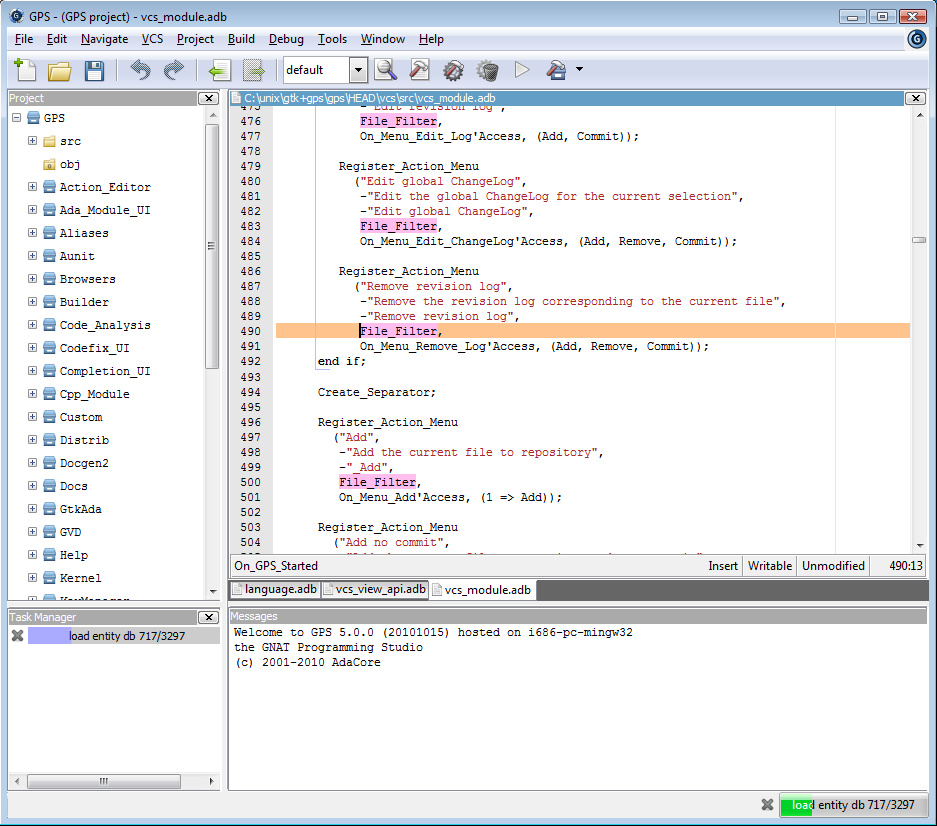
\includegraphics{main-gps.jpg}


\chapter{Description of the Main Windows}
\label{main_window:description-of-the-main-windows}\label{main_window::doc}
\index{main windows}

\section{The Welcome Dialog}
\label{main_window:index-0}\label{main_window:the-welcome-dialog}\label{main_window:id1}
\index{welcome dialog}
\index{screen shot}
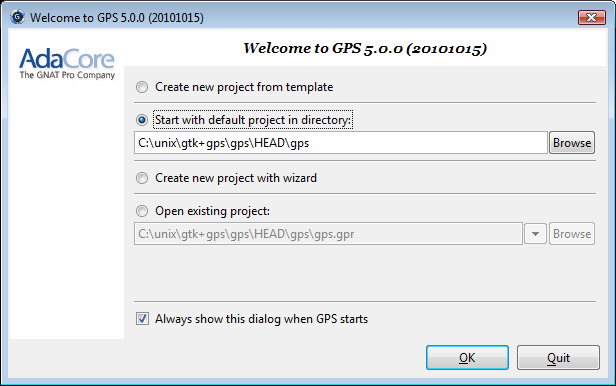
\includegraphics{welcome.jpg}

When starting GPS, a welcome dialog is displayed by default, giving the
following choices:
\begin{description}
\item[{\emph{Create new project from template}}] \leavevmode
If you select this option and then click the \emph{OK} button, GPS will
launch an assistant to create a project using one of the predefined project
templates.

\item[{\emph{Start with default project in directory}}] \leavevmode
\index{project}
If you select this option and click on the \emph{OK} button, GPS will
first look for a project called \code{default.gpr} in the current directory
and load it if found. Otherwise, it will copy in
the current directory the default project found under
\code{\textless{}prefix\textgreater{}/share/gps/default.gpr} and load it.
GPS will remove this copy when exiting or loading another project, if the
copy has not been modified during the session.

If the current directory is not writable, GPS will instead load directly
\emph{\textless{}prefix\textgreater{}/share/gps/readonly.gpr}. In this case, GPS will work in a
degraded mode, where some capabilities will not work (such as building and
source navigation).

\item[{\emph{Create new project with wizard}}] \leavevmode
\index{project}
Selecting this option and clicking on the \emph{OK} button will start a
wizard allowing you to specify most of the properties for a new project. Once
the project is created, GPS will save it and load it automatically.
See {\hyperref[projects:the-project-wizard]{\emph{The Project Wizard}}} for more details on the project wizard.

Several kinds of wizard are available. Depending on the kind of project,
you will get asked different type of information. In the end, GPS will create
one or more project files, and automatically load them.

One of the wizard, ``From existing Ada sources'', will try and import a set of
sources and object files, and attempt to create one or more project files so
that building your application through these project files will put the
objects in the same directory they are currently in. If you have not compiled
your application when launching this wizard, GPS will create a single project
file and all object files will be put in the same object directory. This is
the prefered method when importing sources with duplicate file names, since
the latter is only authorized in a single project file, not across various
project files.

\item[{\emph{Open existing project}}] \leavevmode
\index{project}
You can select an existing project by clicking on the \emph{Browse} button,
or by using a previously loaded project listed in the combo box. When a
project is selected, clicking on the \emph{OK} button will load this
project and open the main window.

\item[{\emph{Always show this dialog when GPS starts}}] \leavevmode
If unset, the welcome dialog won't be shown in future sessions.
In this case, GPS will behave as follows: it will first look for a
\emph{-P} switch on the command line, and load the corresponding project if
present.
Then, it will look for a project file in the current directory and will
load the first project file found.

If no project file can be found in the current directory, GPS will start
with the default project.

To reset this property, go to the menu \emph{Edit-\textgreater{}Preferences}.
.. index:: preferences

{\hyperref[extending:the-preferences-dialog]{\emph{The Preferences Dialog}}}.

\item[{\emph{Quit}}] \leavevmode
If you click on this button, GPS will terminate immediately.

\end{description}

\index{command line}
When you specify a -P switch on the command line, or if there is only one
project file in the current directory, GPS will start immediately with
the project file specified, instead of displaying the welcome dialog.

In addition, if you specify source files on the command line, GPS will also
start immediately, using the default project if no project is specified.

By default, files specified on the command line are taken as is and can
be absolute or relative pathnames. In addition, if you prepend a filename
with the \emph{=} character, then GPS will look for the file in the source
search path of the project.


\section{The Tip of the Day}
\label{main_window:the-tip-of-the-day}\label{main_window:id2}
\index{tip of the day}
This dialog displays short tips on how to make the most efficient use of
GPS. You can click on the \emph{Previous} and \emph{Next} buttons to access
all tips, and close the dialog by either clicking on the \emph{Close} button
or pressing the \code{ESC} key.

You can also disable this dialog by unchecking the \emph{Display Tip of the Day on startup} check box. If you would like to reenable this dialog, you
can go to the \emph{Edit-\textgreater{}Preferences} dialog.

\index{preferences}
\index{screen shot}
{\hyperref[extending:the-preferences-dialog]{\emph{The Preferences Dialog}}}.

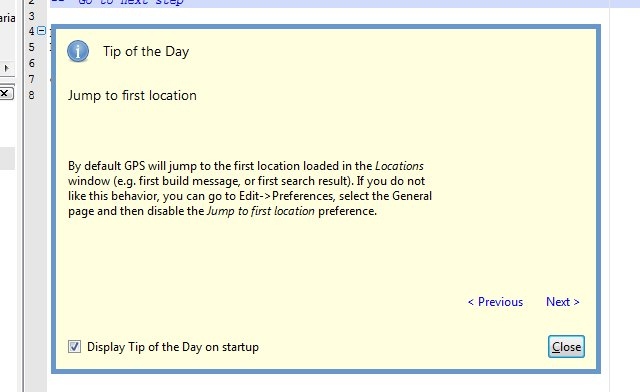
\includegraphics{tip-of-the-day.jpg}


\section{The Menu Bar}
\label{main_window:the-menu-bar}\label{main_window:id3}
\index{menu bar}
This is a standard menu bar that gives access to all the global
functionalities of GPS. It is usually easier to access a given functionality
using the various contextual menus provided throughout GPS: these menus
give direct access to the most relevant actions given the current context
(e.g. a project, a directory, a file, an entity, ...). Contextual menus
pop up when the right mouse button is clicked or when using the special
\code{open contextual menu} key on most PC keyboards.

The menu bar gives access to the following items:
\begin{description}
\item[{\emph{File}}] \leavevmode
{\hyperref[editing:the-file-menu]{\emph{The File Menu}}}.

\item[{\emph{Edit}}] \leavevmode
{\hyperref[editing:the-edit-menu]{\emph{The Edit Menu}}}.

\item[{\emph{Navigate}}] \leavevmode
{\hyperref[navigation:the-navigate-menu]{\emph{The Navigate Menu}}}.

\item[{\emph{VCS}}] \leavevmode
{\hyperref[vcs:the-vcs-menu]{\emph{The VCS Menu}}}.

\item[{\emph{Project}}] \leavevmode
{\hyperref[projects:the-project-menu]{\emph{The Project Menu}}}.

\item[{\emph{Build}}] \leavevmode
{\hyperref[compilation:the-build-menu]{\emph{The Build Menu}}}.

\item[{\emph{Debug}}] \leavevmode
{\hyperref[debugging:the-debug-menu]{\emph{The Debug Menu}}}.

\item[{\emph{Tools}}] \leavevmode
{\hyperref[tools:the-tools-menu]{\emph{The Tools Menu}}}.

\item[{\emph{SPARK}}] \leavevmode
If the SPARK toolset is installed on your system and available on your
PATH, then this menu is available. See
\emph{Help-\textgreater{}SPARK-\textgreater{}Reference-\textgreater{}Using SPARK with GPS} for more details.

\item[{\emph{CodePeer}}] \leavevmode
If the CodePeer toolset is installed on your system and available on your
PATH, then this menu is available. See your CodePeer documentation for more
details.

\item[{\emph{Window}}] \leavevmode
{\hyperref[mdi:multiple-document-interface]{\emph{Multiple Document Interface}}}.

\item[{\emph{Help}}] \leavevmode
{\hyperref[help:the-help-menu]{\emph{The Help Menu}}}.

\end{description}


\section{The Tool Bar}
\label{main_window:the-tool-bar}\label{main_window:id4}
\index{tool bar}
The tool bar provides shortcuts via buttons to some typical actions:
creating a new file, opening a file, saving the current file;
undo/redo last editing; go to previous/next location;

\index{build}
select build mode, compile file, build project, clean project;

\index{debugger}
start/continue the debugging session, step/next execution, finish
current procedure.

The icon on the far right of the tool bar will be animated to indicate that an
action (e.g. a build or a search) is going on in the background.


\section{The Work Space}
\label{main_window:id5}\label{main_window:the-work-space}
\index{work space}
\index{MDI}
\index{Multiple Document Interface}
The whole work space is based on a multiple document interface,
{\hyperref[mdi:multiple-document-interface]{\emph{Multiple Document Interface}}}.


\section{The Project View}
\label{main_window:the-project-view}
\index{project view}
\index{project view}
\index{project}
The project view provides a representation of the various components of your
project hierarchy, as listed below.
It is displayed by default on the left side of the main window, and can
be selected by using the \emph{Project-\textgreater{}Project View} or
\emph{Tools-\textgreater{}Views-\textgreater{}Project} menu items.

\index{drag-n-drop}
Under Windows, it is possible to drop files (coming e.g. from the Explorer)
in the project view with the following behavior: a project file dropped
will be loaded; any other file will be opened in a new source editor.

\index{screen shot}
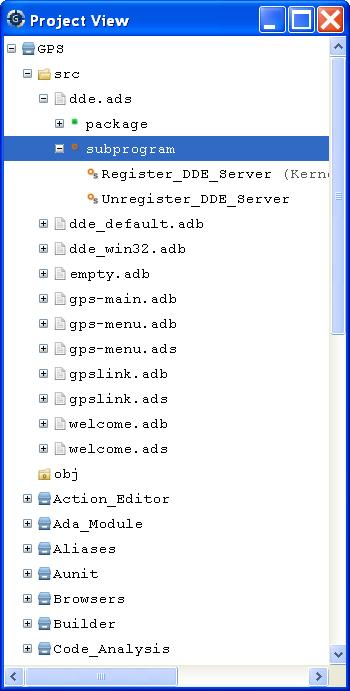
\includegraphics{project-view.jpg}

\index{interactive search}
The project view, as well as the file and outline view provide an
interactive search capability allowing you to quickly
search in the information currently displayed. The default key
to start an interactive search is \code{control-f}.
\phantomsection\label{main_window:interactive-search}
This will open a small window
at the bottom of the view where you can interactively type names.
The first matching name in the tree will be selected while you type it.
You can then also use the \code{up} and \code{down} keys to navigate through
all the items matching the current text.

The various components that are displayed are:
\begin{description}
\item[{\emph{projects}}] \leavevmode
\index{project view}
All the sources you are working with are put under
control of projects. These projects are a way to store the switches to
use for the various tools, as well as a number of other properties.

They can be organized into a project hierarchy, where a root project
can import other projects, with their own set of sources.

Initially, a default project is created, that includes all the sources
in the current directory.

The \emph{Project View} displays this project hierarchy: the top node
is the root project of your application (generally, this is where the
source file that contains the main subprogram will be located). Then a node
is displayed for each imported project, and recursively for their own imported
projects.

A given project might appear multiple times in the
\emph{Project View}, if it is imported by several other projects.

There exists a second display for this project view, which lists all projects
with no hierarchy: all projects appear only once in the view, at the top
level. This display might be useful for deep project hierarchies, to make it
easier to find projects in the project view.

\index{Show flat view}
This display is activated through the contextual menu entry
\emph{Show flat view}, which acts as a switch between the two displays.

A special icon with a pen mark is displayed if the project
was modified, but not saved yet. You can choose to save it at any time
by right-clicking on it. GPS will remind you to save it before any
compilation, or save it automatically, if the corresponding preference
is saved.

\end{description}

\emph{directories}
\begin{quote}

\index{directory}
\index{Windows}
The files inside a project can be organized into several physical
directories on the disk. These directories are displayed under each
project node in the \emph{Project View}

\index{Show absolute paths}
You can chose whether you want to see the absolute path names for the
directories or paths relative to the location of the project. This is done
through the \emph{Show absolute paths} contextual menu.

Special nodes are created for object and executables directories. No
files are shown for these.

\index{Show hidden directories}
The contextual menu entry \emph{Show hidden directories} can be used to filter
the directories considered as hidden. This can be used to not display the
version control directories like \code{CVS} or \code{.svn} for example.
\end{quote}

\emph{files}
\begin{quote}

\index{file}
\index{file view}
The source files themselves are stored in the directories, and
displayed under the corresponding nodes. Note that
only the source files that actually belong to the
project (i.e. are written in a language supported by that project and
follow its naming scheme) are actually visible.
For more information on supported languages, {\hyperref[projects:supported-languages]{\emph{Supported Languages}}}.

A given file might appear multiple times in the \emph{Project View},
if the project it belongs to is imported by several other projects.

If you left click on a file and keep the button pressed, you can drop it
anywhere in GPS to open an editor at that location.
\end{quote}

\emph{entities}
\begin{quote}

\index{entity}
If you open the node for a source file, the file is parsed by one of the
fast parsers integrated in GPS so that all entities declared in
the project can be shown. These entities are grouped into various
categories, which depend on the language. Typical categories include
subprograms, packages, types, variables, tasks, ...
\end{quote}

Double-clicking on a file, or simple clicking on any entity will open
a source editor and display respectively the first line in this file
or the line on which the entity is defined.

You can also drag a file anywhere into GPS. This will open a new editor
if the file is not already edited, or move the existing editor otherwise.
If you press \code{shift} at the same time, and the file is already edited,
a new view of the existing editor is created instead.

\index{search}
\index{find}
If you open the search dialog through the \emph{Navigate-\textgreater{}Find or Replace...}
menu, you have the possibility to search for anything in the project view,
either a file or an entity. Note that searching for an entity can be slow
if you have lots of files, and/or big files.

\index{view}
\index{locate in project view}
A contextual menu, named \emph{Locate in Project View}, is also provided when
inside a source editor. This will automatically search for the first entry for
this file in the project view. This contextual menu is also available in other
modules, e.g. when selecting a file in the \emph{Dependency Browser}.


\subsection{The configuration variables}
\label{main_window:the-configuration-variables}
\index{configuration variable}
\index{project variable}
\index{variable}
\index{GNAT}
\index{project file}
\index{project}
As described in the GNAT User's Guide, the project files can be
configured through external variables (typically environment
variables). This means that e.g. the exact list of source files, or the
exact switches to use to compile the application can be changed when
the value of these external variables is changed.

GPS provides a simple access to these variables, through a window
called the \emph{Scenario View}. These variables are called
\emph{Configuration Variables}, since they provide various scenarios for
the same set of project files.

\index{screen shot}
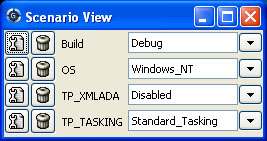
\includegraphics{scenario-view.jpg}

A combo box is displayed in this area for each environment
variable the project depends on. The current value of the variable can
be set simply by selecting it from the pop-down window that appears
when you click on the arrow on the right of the variable name

\index{project view}
New variables can be added through the contextual menu
\emph{Project-\textgreater{}Add Configuration Variable} in the \emph{Project View}.
The list of possible values for a variable can be changed by clicking on the
button on the left of the variable's name.

Whenever you change the value of one of the variables, the project is
automatically recomputed, and the list of source files or directories
is changed dynamically to reflect the new status of the
project. Starting a new compilation at that point will use the new
switches, and all the aspects of GPS are immediately affected
according to the new setup.


\subsection{Icons for source language entities}
\label{main_window:icons-for-source-language-entities}
\index{icons for source language entities}
Entities in the source code are presented with representative icons within the
various GPS views (the \emph{Outline}, \emph{Project}, and \emph{Entity} views, for example).
These icons indicate both the language categories of the entities, such as
packages and methods, as well as compile-time visibility.  In addition, the
icons distinguish entity declarations from other entities.  The same icons are
used for all programming languages supported by the viewers, with
language-specific interpretations for both compile-time visibility and
recognizing declarations.

There are five language categories used for all supported languages: \emph{package},
\emph{subprogram}, \emph{type}, \emph{variable}, and \emph{generic}.  The icons corresponding to
these language categories are as follows.
\begin{itemize}
\item {} 
The \emph{package} category's icon is a square.


\includegraphics{square_x.png}

\item {} 
The \emph{subprogram} category's icon is a circle.


\includegraphics{circle_x.png}

\item {} 
The \emph{type} category's icon is a triangle.


\includegraphics{triangle_x.png}

\item {} 
The \emph{variable} category's icon is a dot.


\includegraphics{dot_x.png}

\item {} 
The \emph{generic} category's  icon is a diamond.


\includegraphics{diamond_x.png}

\end{itemize}

These basic icons are enhanced with decorators, when appropriate, to indicate
compile-time visibility constraints and to distinguish declarations from
completions. For example, the icons for entity declarations have a small `S'
decorator added, denoting a `spec'.

With respect to compile-time visibility, icons for `protected' and `private'
entities appear within an enclosing box indicating a visibility constraint. For
entities with `protected' visibility, this enclosing box is colored in gray.
`Private' entities are enclosed within a red box.  The icons for `public'
entities have no such enclosing box. For example, a variable with `private'
visibility would be represented by an icon consisting of a dot enclosed within
a red box.

These additional decorators are combined when appropriate. For example, the
icon corresponding to the `private' declaration of a `package' entity would be
a square, as for any package entity, with a small `S' added, all enclosed
within a red box.

Language constructs are mapped to the categories in a language-specific manner.
For example, C++ namespaces and Ada packages correspond to the \emph{package}
category.  C functions and Ada subprograms correspond to the \emph{method} category,
and so on.  The \emph{generic} category is a general category representing other
language entities, but note that not all possible language constructs are
mapped to categories and icons.  (Note also that the \emph{generic} category does
not correspond to Ada generic units or C++ templates.)

The names of the categories should not be interpreted literally in terms of
language constructs because the categories are rather general, in order to
limit the number used. The \emph{variable} category includes both constants and
variables in Ada, for example. Limiting the number of categories maintains a
balance between presentation complexity and the need to support distinct
programming languages.

Icons for a given entity may appear more than once within a view. For example,
an Ada private type will have both a partial view in the visible part of the
enclosing package as well as a full view in the private part of the package.
Two triangle icons will therefore appear for the two occurrences of the type
name, one with the additional decorator indicating the `private' compile-time
visibility.


\section{The File View}
\label{main_window:id6}\label{main_window:the-file-view}
\index{File View}
In addition to the \emph{Project View}, GPS also provides a
\emph{File View} through the \emph{Tools-\textgreater{}Views-\textgreater{}Files} menu.

\index{screen shot}
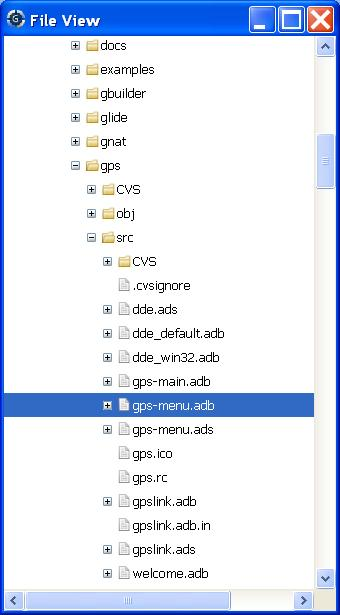
\includegraphics{file-view.jpg}

In this view, directories are displayed exactly as they are organized
physically on the disk (including Windows drives).

By default, the \emph{File View} will display all the files that exist on the disk.
Filters can be set through the contextual menu to only show the files and
directories that belong to the project hierarchy by using the contextual menu
\emph{Show files from project only}.

Each source file can also be explored as described in {\hyperref[projects:the-project-view]{\emph{The Project View}}}.
Drag and drop of files is also possible from the files view, to conveniently
open a file.

The contextual menu also allow you to create, rename and delete files and
directories. Some of those operations are also available from the Project View.


\section{The Entity View}
\label{main_window:the-entity-view}\label{main_window:id7}
\index{Entity View}
GPS provides an \emph{Entity View} which allows you to browse and quickly find all
Ada entities referenced in the currently loaded project hierarchy. This view
can be accessed through the \emph{Tools-\textgreater{}Views-\textgreater{}Entities} menu.

\index{screen shot}
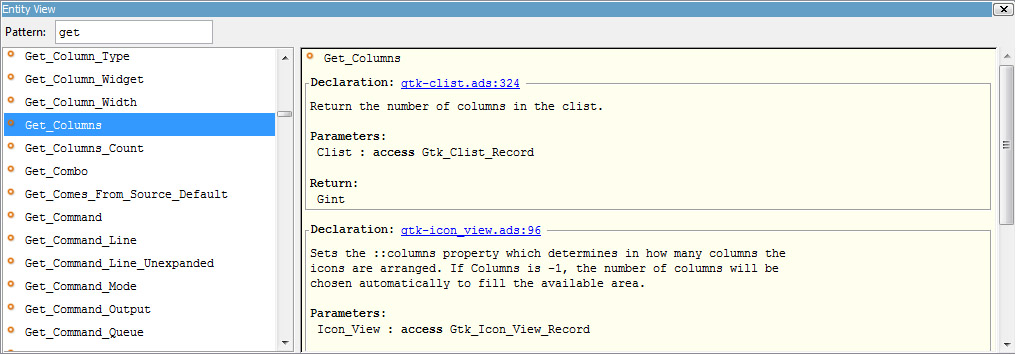
\includegraphics{entity-view.jpg}

This view is divided in three parts: a \emph{Pattern} entry, a tree view, and a
documentation view.

To query an entity, enter a search pattern in the \emph{Pattern} entry. The tree
view then shows a list of all known entities which start with this pattern.
When an entry is selected in the tree, the documentation view displays the
documentation corresponding to the selected entity.

When the \emph{File View} has the focus, using the up/down arrow keys changes the
selection in the tree, and pressing the Enter key opens an editor to the
declaration of the selected entity. It is also possible to jump to this
location by double-clicking on the line in the tree, or by clicking on the
hyperlink in the documentation view.

Note that the view shows the entities that are currently loaded in memory, see
{\hyperref[navigation:support-for-cross-references]{\emph{Support for Cross-References}}}.


\section{The Window View}
\label{main_window:the-window-view}\label{main_window:id8}
\index{Window View}
The \emph{Window View} displays the currently opened windows.  It is opened through
the \emph{Tools-\textgreater{}Views-\textgreater{}Windows} menu.

It can display the opened windows in one of two ways:
\begin{itemize}
\item {} 
Sorted alphabetically

\item {} 
Organized by notebooks, as in the GPS window itself. This latter view
is mostly useful if you have lots of windows open

\end{itemize}

The mode is selected through the contextual menu.

You can also choose, through this contextual menu, whether only the source
editors should be visible, or whether all windows should be displayed.

This window allows you to quickly select and focus on a particular window, by
clicking on the corresponding line with the left mouse button. If you click and
leave the mouse button pressed, this starts a drag and drop operation so that
you can also move the window to some other place in the desktop (see the
description of the MDI earlier in this document).

Multiple windows can be selected by clicking with the mouse while pressing the
control or shift keys. The Window view provides a contextual menu to easily
close all selected windows at once, which is a very fast way to cleanup your
desktop after you have finished working on a task.


\section{The Outline View}
\label{main_window:the-outline-view}\label{main_window:id9}
\index{Outline View}
The Outline View, which you can choose to activate through the
\emph{Tools-\textgreater{}Views-\textgreater{}Outline} menu, shows the contents of the current file.

\index{screen shot}
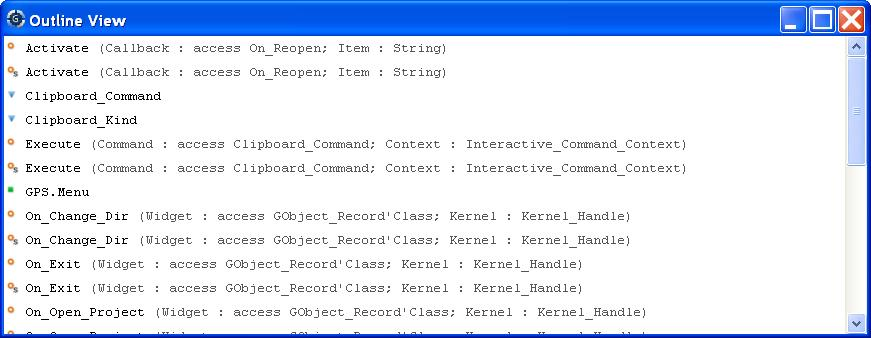
\includegraphics{outline-view.jpg}

The exact meaning of this depends on the language you are seeing. For Ada, C
and C++ files, this is the list of entities that are declared at the global
level in your current file (Ada packages, C++ classes, subprograms, Ada types,
...).

Clicking on any entity in this view will automatically jump to the right line
in the file, including if your file has been slightly modified since the
outline view was last refreshed.

To refresh the contents of the view, select the \emph{Refresh} entry in the
contextual menu (right-click anywhere in the outline view).  The Outline View
is updated automatically after editing, saving the file, or switching to a
different editor.

There are several preferences associated with the
{\hyperref[extending:outline-preferences]{\emph{outline view}}}.


\section{The Clipboard View}
\label{main_window:the-clipboard-view}\label{main_window:id10}
\index{clipboard view}
GPS has an advanced mechanism for handling copy/paste operations.

When you select the menus \emph{Edit-\textgreater{}Copy} or \emph{Edit-\textgreater{}Cut}, GPS adds the current
selection to the clipboard. As opposed to what lots of applications do, it
doesn't discard the previous contents of the clipboard, but save it for future
usage. It saves a number of entries this way, up to 10 by default.  This value
is configurable through the \emph{Clipboard Size} preference.

When you select the menu \emph{Edit-\textgreater{}Paste}, GPS will paste the last entry made in
the clipboard at the current location in the editor.

If you immediately select \emph{Edit-\textgreater{}Paste Previous}, this newly inserted text will
be removed, and GPS will instead insert the second to last entry added to the
clipboard. You can keep selecting the same menu to get access to older entries.

This is a very powerful mechanism, since it means you can copy several distinct
lines from a place in an editor, move to an other editor and paste all these
separate lines, without having to go back and forth between the two editors.

The \emph{Clipboard View} provides a graphical mean of seeing what is currently
stored in the clipboard. It appears as a list of lines, each of which is
associated with one level of the clipboard. The text that shows in these lines
is the first line of the selection at that level that contains non blank
characters. Leading characters are discarded. \emph{{[}...{]}} is prepended or appended
in case the selection has been truncated.

If you bring the mouse over a line in the \emph{Clipboard View}, a tooltip will pop
up showing the entire selection corresponding to the line by opposition to the
possibly truncated one.

In addition, one of the lines has an arrow on its left. This indicates the line
that will be pasted when you select the menu \emph{Edit-\textgreater{}Paste}. If you select
instead the menu \emph{Edit-\textgreater{}Paste Previous}, then the line below that one will be
inserted instead.

If you double-click on any of these lines, GPS will insert the corresponding
text in the current editor, and make the line you clicked on the current line,
so that selecting \emph{Edit-\textgreater{}Paste} or the equivalent shortcut will now insert that
line.

The contextual menu in the clipboard view provides one entry, which is \emph{Append
To Previous}. If you select this entry, the select line will be append to the
one below, and removed from the clipboard. This means that selection
\emph{Edit-\textgreater{}Paste} will in fact paste the two entries at the same time. This is in
particular useful when you want to copy lines from separate places in the
initial file, merge them, and then paste them together one or more times later
on, through a single operation.

The Clipboard View content is preserved between GPS sessions. As an exception,
huge entries are removed and replaced with an entry saying ``{[}Big entry has been
removed{]}''.


\section{The Callgraph View}
\label{main_window:id11}\label{main_window:the-callgraph-view}
\index{callgraph}
The callgraph view plays a role similar the callgraph browser. They display the
same information about entities, but in two different ways: the callgraph view
displays the information in a tree, easily navigable and perhaps easier to
manipulate when lots of entities are involved; the callgraph browser displays
the information as graphical boxes that can be manipulated on the screen, and
is best suited to generate a diagram that can be later exported to your own
documents.

This callgraph view is used to display the information about what subprograms
are called by a given entity, and, opposite, what entities are calling a given
entity.

Some references might be reported with an additional '' (dispatching)'' text.  In
such a case, this indicates that the call to the entity is not explicit in the
sources, but could occur through dynamic dispatching. This of course depends on
what arguments are passed to the caller at run time, and it is possible that
the subprogram is in fact never dispatched to.

This view is automatically displayed when you select one of the contextual
menus \emph{... calls} and \emph{... is called by}. Every time you select one of these
menus, a new view is opened to display that entity.

Whenever you expand a node from the tree by clicking on the small expander
arrow on the left of the line, further callgraph information is computed for
the selected entity, which makes it very easy to get information for a full
callgraph tree.

Closing and expanding a node again will recompute the callgraph for the entity.

On the right side of the main tree, a list displays the locations of calls for
the selected entity. Clicking on entries in this list opens editors showing the
corresponding location.

The Callgraph View supports keyboard navigation: \emph{Up} and \emph{Down} keys navigate
between listed locations, \emph{Left} collapses the current level, \emph{Right} expands
the current level, and \emph{Return} jumps to the currently selected location.

The callgraph view is automatically saved in the desktop, and restored the next
time you restart GPS. However, the information displayed in these might no
longer be accurate at this stage, since it shows the status of the callgraph
during the last GPS session.

Left-clicking on a line in the Call Tree brings up a contextual menu with the
following entries:
\begin{description}
\item[{\emph{Collapse all}}] \leavevmode
Collapse all the entities in the Callgraph View.

\item[{\emph{Remove entity}}] \leavevmode
Remove the selected entity from the Callgraph View.

\item[{\emph{Clear Call Trees}}] \leavevmode
Remove all entries from the Callgraph View.

\end{description}


\section{Bookmarks}
\label{main_window:bookmarks}\label{main_window:id12}
\index{bookmark}
Bookmarks are a convenient way to remember places in your code or in your
environment so that you can go back to them at any point in the future.  These
bookmarks are saved automatically whenever they are modified, and restored when
GPS is reloaded, so that they exist across GPS sessions.

Bookmarks will automatically remember the exact location in an editor, not in
terms of line/column, but in terms of which word they point to. If you modify
the file through GPS, the bookmark will be automatically updated to keep
refering to the same place. Likewise if you close and reopen the file.
However, when the file is modified outside of GPS, the bookmark will not be
aware of that change, and will thus reference another place in the file.

The menu \emph{Edit-\textgreater{}Create Bookmark} allows you to create a bookmark at the current
location (either in the editor, or the browser for instance).

All the bookmarks you have created will be visible in the
\emph{Tools-\textgreater{}Views-\textgreater{}Bookmarks} window. Clicking on the small icon to the left side
of each line will immediately jump to that bookmark.

You can rename a bookmark so that it is easier to remember what it refers to.
To do so, open the Bookmarks window, and click twice on the line of the
bookmark. This will change the way the name is displayed, so that you can edit
it in place. Press \code{enter} when you are done modifying the name.

You can delete an existing bookmark by right clicking on the line, and select
\emph{Delete bookmark} in the contextual menu.


\section{The Messages Window}
\label{main_window:the-messages-window}\label{main_window:id13}
\index{messages}
\index{messages window}
\index{build}
\index{errors}
The Messages window is used by GPS to display information and feedback about
operations, such as build output, information about processes launched, error
messages.

\index{screen shot}
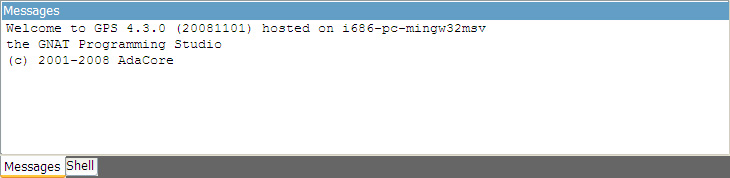
\includegraphics{messages.jpg}

This is a read-only window, which means that only output is available, no input
is possible.

\index{execution window}
\index{execution}
\index{shell window}
\index{shell}
For an input/output window, see {\hyperref[main_window:the-execution-window]{\emph{The Execution Window}}} and also
{\hyperref[main_window:the-shell-and-python-windows]{\emph{The Shell and Python Windows}}}.


\section{The Shell and Python Windows}
\label{main_window:the-shell-and-python-windows}\label{main_window:id14}
\index{python window}
\index{shell}
\index{shell window}
\index{interactive command}
\index{command}
These windows give access to the various scripting languages supported by GPS,
and allow you to type commands such as editing a file or compiling without
using the menu items or the mouse.

An OS shell window is now also available in GPS, providing a simple access to
the underlying OS shell as defined by the \emph{SHELL} or \emph{COMSPEC} environment
variables.

To show the shell consoles, select the menu \emph{Tools-\textgreater{}Consoles}.

See {\hyperref[extending:scripting-gps]{\emph{Scripting GPS}}} for more information on using scripting languages
within GPS.

\index{screen shot}
\index{key}
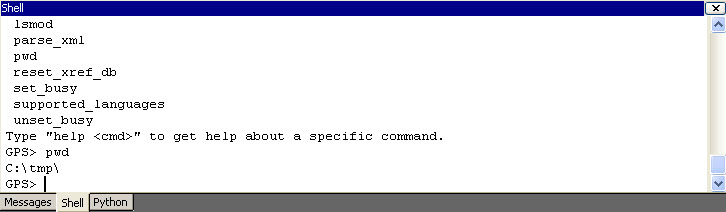
\includegraphics{shell-window.jpg}

You can use the \code{up} and \code{down} keys to navigate through the history
of commands.


\section{The Locations View}
\label{main_window:id15}\label{main_window:the-locations-view}
\index{location}
\index{locations view}
\index{search}
\index{compilation}
\index{build}
The Location Tree is filled whenever GPS needs to display a list of locations
in the source files (typically, when performing a global search, compilation
results, and so on).

\index{screen shot}
\index{category}
\index{file}
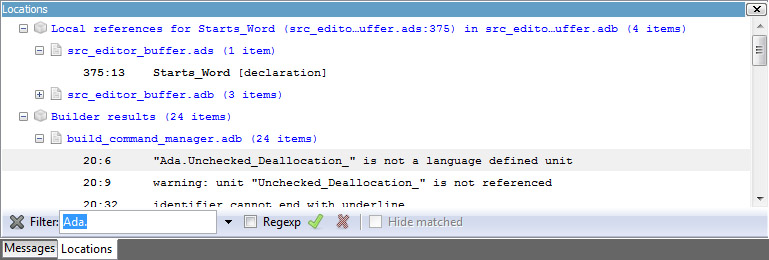
\includegraphics{locations-view.jpg}

The Locations View shows a hierarchy of categories, which contain files, which
contain locations. Clicking on a location item will bring up a file editor at
the requested place. Right-clicking on file or category items brings up a
contextual menu allowing you to remove the corresponding node from the view.
Placing the mouse over an item automatically pop up a tooltip window with full
text of the item if this text can't be completely shown in the window.

Every time a new category is created, as a result of a compilation or a search
operation for example, the first entry of that category is automatically
selected, and the corresponding editor opened. This behavior can be controlled
through a preference \emph{Jump To First Location}.

Closing the Locations view will remove from the editors locations that are also
visible in the Locations view.  If the Locations View is present when exiting
GPS and the desktop is saved, the locations will be saved as part of the
desktop for the current project, and will be loaded the next time GPS is
started on the same project.

\index{key}
\index{menu}
To navigate through the next and previous location (also called \emph{Tag}), you can
use the menu items \emph{Navigate-\textgreater{}Previous Tag} and \emph{Navigate-\textgreater{}Next Tag}, or the
corresponding key bindings.

Left-clicking on a line in the Location Tree brings up a contextual menu with
the following entries:
\begin{description}
\item[{\emph{Filter panel}}] \leavevmode
Controls availability of the filter panel at the bottom of the window.

\item[{\emph{Sort by subcategory}}] \leavevmode
Toggle the sorting of the entries by sub-categories. This is useful,
for example, for separating the warnings from the errors in the build
results.

\item[{\emph{Expand category}}] \leavevmode
Expand all the files in the current categories.

\item[{\emph{Collapse all}}] \leavevmode
Collapse all the categories in the Locations View

\item[{\emph{Remove category/file/message}}] \leavevmode
Remove the selected category, file or message from the Locations View.
Selected message can be removed using \emph{Locations view-\textgreater{}Remove message}
key binding also.

\item[{\emph{Export messages into text file}}] \leavevmode
Export all messages of the selected category/file into text file.

\item[{\emph{Jump to location}}] \leavevmode
Open the location contained in the message, if any.

\item[{\emph{Clear Locations View}}] \leavevmode
Remove all entries from the Locations View.

\end{description}

In some cases, a wrench icon will be associated on the left of a compilation
message. See {\hyperref[tools:code-fixing]{\emph{Code Fixing}}} for more information on how to make advantage
of this icon.

The filter panel can be used to filter messages which match (or do not match) a
text pattern or regular expression. As soon as you type in the text entry, the
filter is enabled. If you clear the text, the filter is disabled.  The \emph{Close}
button on the filter panel hides it and cancels the filter.  The \emph{Regexp} check
button specifies how to use the filter text entry: as plain text or regular
expression.  The \emph{Hide matched} check button reverts the filter, e.g. switch
between matching and non-matching items.


\section{The Execution Window}
\label{main_window:the-execution-window}\label{main_window:id16}
\index{execution}
\index{execution window}
\index{run}
Each time a program is launched using the menu \emph{Build-\textgreater{}Run}, a new execution
window is created to provide input and output for this program.

In order to allow post mortem analysis and copy/pasting, the execution windows
are not destroyed when the application terminates.

\index{key}
\index{menu}
To close an execution window, click on the cross icon on the top right corner
of the window, or use the menu \emph{File-\textgreater{}Close}, or the menu \emph{Window-\textgreater{}Close} or
the key binding \code{Ctrl-W}.

If you close the execution window while the application is still running, a
dialog window is displayed, asking whether you want to kill the application, or
to cancel the close operation.


\section{The Status Line}
\label{main_window:the-status-line}\label{main_window:id17}
\index{status}
\index{status line}
\index{status bar}
\index{progress bar}
The status line is composed of two areas: on the left a status bar and on the
right a progress bar (displayed only when background tasks are running).

\index{build}
The progress bar is used to display information about on going operations such
as builds, searches, or VCS commands. These tasks operate in the background,
and can be paused/resumed by double clicking on the progress bar: this will
open {\hyperref[main_window:the-task-manager]{\emph{The Task Manager}}}.  In addition, you can click on the \emph{close} icon
on the left of the progress bar to interrupt the running task.


\section{The Task Manager}
\label{main_window:id18}\label{main_window:the-task-manager}
\index{tasks}
\index{background tasks}
\index{task manager}
The Task Manager window lists all the currently running GPS operations that run
in the background, such as builds, searches or VCS commands.

The Task Manager is opened by double clicking on the progress bar or using the
\emph{Tools-\textgreater{}Views-\textgreater{}Tasks} menu, and can be put anywhere in your desktop.

For each of these tasks, the Task Manager shows the status of the task, and the
current progress. The execution of theses tasks can be suspended using a
contextual menu, brought up by right-clicking on a line.

When exiting GPS, if there are tasks running in the Task Manager, a window will
display those tasks. You can also bring up a contextual menu on the items in
this window.  You can force the exit at any time by pressing the confirmation
button, which will kill all remaining tasks, or continue working in GPS by
pressing the Cancel button.

\index{screen shot}
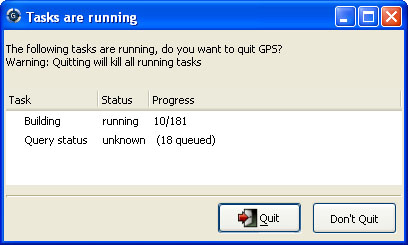
\includegraphics{task-manager.jpg}


\chapter{Online Help}
\label{help:online-help}\label{help::doc}\label{help:id1}
\index{Online help}
\index{help}
\index{HTML}
By default when you start GPS, the working area contains a welcome page giving
a few starting points in the online help.

Online help for the GNAT tools is available from the \emph{Help} menu item.  GPS
launches an external html browser to view these pages. (See
{\hyperref[extending:the-preferences-dialog]{\emph{The Preferences Dialog}}} on how to configure this under Unix. Under
Windows systems, the default HTML browser is used.)


\section{The Help Menu}
\label{help:the-help-menu}\label{help:id2}
The Help menu item provides the following entries:
\begin{description}
\item[{\emph{Welcome}}] \leavevmode
Open the GPS Welcome page.

\item[{\emph{Contents}}] \leavevmode
Open a special HTML file that contains links for all the
documentation files currently registered in GPS, {\hyperref[help:adding-new-help-files]{\emph{Adding New Help Files}}}.

\item[{\emph{GPS}}] \leavevmode
Submenu containing GPS documentation items.

\item[{\emph{GNAT Runtime}}] \leavevmode
Submenu referencing all GNAT run-time files available, and a direct access
to the corresponding specs containing embedded documentation.

\item[{\emph{Python extensions}}] \leavevmode
Gives access to the GPS API available via python.

\item[{\emph{About}}] \leavevmode
Display a dialog giving information about the versions of GPS and GNAT used:

\index{screen shot}
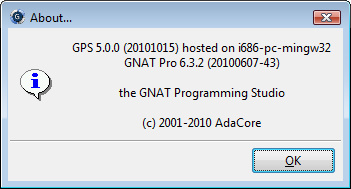
\includegraphics{about.jpg}

\end{description}

This menu contains a number of additional entries, depending on what
documentation packages were installed on your system. See the next section to
see how to add new help files.


\section{Adding New Help Files}
\label{help:adding-new-help-files}\label{help:id3}
\index{gps\_index.xml}
GPS will search for the help files in the list of directories set in the
environment variable \emph{GPS\_DOC\_PATH} (a colon-separated list of directories on
Unix systems, or semicolon-separated list of directories on Windows systems).
In addition, the default directory \emph{\textless{}prefix\textgreater{}/share/doc/gps/html} is also
searched. If the file cannot be found in any of these directories, the
corresponding menu item will be disabled.

The environment variable \emph{GPS\_DOC\_PATH} can either be set by each user in his
own environment, or can be set system-wide by modifying the small wrapper
script \code{gps} itself on Unix systems.

It can also be set programmatically through the GPS shell or any of the
scripting languages. This is done with:

\begin{Verbatim}[commandchars=\\\{\}]
\PYG{n}{GPS}\PYG{o}{.}\PYG{n}{add\PYGZus{}doc\PYGZus{}directory} \PYG{p}{(}\PYG{l+s}{"}\PYG{l+s}{/home/foo}\PYG{l+s}{"}\PYG{p}{)}
\end{Verbatim}

The specific list of files shown in the menus is set by reading the index files
in each of the directories in \emph{GPS\_DOC\_PATH}. These index files must be called
\code{gps\_index.xml}.

The format of these index files is specified in {\hyperref[extending:adding-documentation]{\emph{Adding documentation}}}.


\chapter{Multiple Document Interface}
\label{mdi:id1}\label{mdi::doc}\label{mdi:multiple-document-interface}
\index{MDI}
\index{Multiple Document Interface}
\index{window manager}
\index{work space}
All the windows that are part of the GPS environment are under control of what
is commonly called a multiple document interface (MDI for short). This is a
common paradigm on windowing systems, where related windows are put into a
bigger window which is itself under control of the system or the windows
manager.

This means that, by default, no matter how many editors, browsers, views, ...
windows you have opened, your system will still see only one window (On Windows
systems, the task bar shows only one icon). However, you can organize the GPS
windows exactly the way you want, all inside the GPS main window.

This section will show the various capacities that GPS provides to help you
organize your workspace.


\section{Selecting Windows}
\label{mdi:id2}\label{mdi:selecting-windows}
\index{window selection}
At any time, there is only one selected window in GPS (the \textbf{active window}).
You can select a window either by clicking in its title bar, which will then
get a different color, or by selecting its name in the menu \emph{Window}.

Alternatively, windows can be selected with the keyboard. By default, the
selection key is \code{Alt-Tab}. When you press it, a temporary dialog is
popped-up on the screen, with the name of the window that will be selected when
the key is released. If you press the selection key multiple times, this will
iterate over all the windows currently open in GPS.

This interactive selection dialog is associated with a filter, displayed below
the name of the selected window. If you maintain \code{Alt} pressed while
pressing other keys than \code{Tab}, this will modify the current filter. From
then on, pressing \code{Alt-Tab} will only iterate through those windows that
match the filter.

The filter is matched by any window whose name contains the letter you have
typed. For instance, if you are currently editing the files \code{unit1.adb}
and \code{file.adb}, pressing \code{t} will only leave \code{unit1.adb}
selectable.


\section{Closing Windows}
\label{mdi:id3}\label{mdi:closing-windows}
\index{close}
\index{title bar}
Wherever the windows are displayed, they are always closed in the same manner.
In the right side of the title bar of the window, one small button is
displayed, looking like a cross. Clicking on this button will close the window.

An alternative way to close the window is to double-click on the icon to the
left of the title bar of the window. Not all windows have such an icon, but
editors do for instance.

When a window is closed, the focus is given to the window of the same part of
the MDI (each of the docks or the middle area) that previously had the focus.
Therefore, if you simply open an editor as a result of a cross-reference query,
you can simply close that editor to go back to where you were before.

Alternatively, you can also select the window by clicking anywhere in its title
bar, and then select the menu \emph{Window-\textgreater{}Close}.

Finally, a window can be closed by right-clicking in the associated notebook
tab (if the tabs are visible), and select \emph{Close} in the contextual menu.

In the notebook tab (when you are in an editor), you will also find a \emph{Close
all other editors} menu, which, as its name implies, will keep a single editor
open, the one you are clicking on.


\section{Splitting Windows}
\label{mdi:splitting-windows}\label{mdi:id4}
\index{Splitting}
Windows can be split at will, through any combination of horizontal and
vertical splits.  This feature requires at least two windows (text editors,
browsers, ...) to be superimposed in the central area. Selecting either the
\emph{Window-\textgreater{}Split Horizontally} or \emph{Window-\textgreater{}Split Vertically} menus will then
split the selected window in two. In the left (resp. top) pane, the currently
selected window will be left on its own. The rest of the previously
superimposed windows will be put in the right (resp. bottom) pane. You can then
in turn split these remaining windows to achieve any layout you want.

All split windows can be resized interactively by dragging the handles that
separate them. A preference (menu \emph{Edit-\textgreater{}Preferences}) controls whether this
resizing is done in opaque mode or border mode. In the latter case, only the
new handle position will be displayed while the mouse is dragged.

You may want to bind the key shortcuts to the menus \emph{Window-\textgreater{}Split
Horizontally} as well as \emph{Window-\textgreater{}Split Vertically} using the key manager. In
addition, if you want to achieve an effect similar to e.g. the standard Emacs
behavior (where \code{control-x 2} splits a window horizontally, and
\code{control-x 3} splits a window vertically), you can use the key manager
({\hyperref[extending:the-key-manager-dialog]{\emph{The Key Manager Dialog}}}).

{\hyperref[mdi:moving-windows]{\emph{Moving Windows}}} will show how to do the splitting through drag-and-drop
and the mouse, which in general is the fastest way to do.

Several editors or browsers can be put in the same area of the MDI. In such a
case, they will be grouped together in a notebook widget, and you can select
any of them by clicking on the corresponding tab. Note that if there are lots
of windows, two small arrows will appear on the right of the tabs.  Clicking on
these arrows will show the remaining tabs.

In some cases GPS will change the color and size of the title (name) of a
window in the notebook tab. This indicates that the window content has been
updated, but the window wasn't visible. Typically, this is used to indicate
that new messages have been written in the messages or console window.


\section{Floating Windows}
\label{mdi:floating-windows}\label{mdi:id5}
\index{floating}
\index{top level}
Although the MDI, as described so far, is already extremely flexible, it is
possible that you prefer to have several top-level windows under direct control
of your system or window manager. This would be the case for instance if you
want to benefit from some extra possibilities that your system might provide
(virtual desktops, different window decoration depending on the window's type,
transparent windows, multiple screens, ...).

GPS is fully compatible with this behavior, since windows can also be
\textbf{floating windows}. Any window that is currently embedded in the MDI can be
made floating at any time, simply by selecting the window and then selecting
the menu \emph{Window-\textgreater{}Floating}. The window will then be detached, and can be moved
anywhere on your screen, even outside of GPS's main window.

\index{menu}
There are two ways to put a floating window back under control of GPS.  The
more general method is to select the window through its title in the menu
\emph{Window}, and then unselect \emph{Window-\textgreater{}Floating}.

\index{preferences}
The second method assumes that the preference \textbf{Destroy Floats} in the menu
\emph{Edit-\textgreater{}Preferences} has been set to false. Then, you can simply close the
floating window by clicking in the appropriate title bar button, and the window
will be put back in GPS. If you actually want to close it, you need to click
once again on the cross button in its title bar.

\index{all floating}
A special mode is also available in GPS, where all windows are floating. The
MDI area in the main window becomes invisible. This can be useful if you rely
on windows handling facilities supported by your system or window manager but
not available in GPS. This might also be useful if you want to have windows on
various virtual desktops, should your window manager support this.

This special mode is activated through a preference (menu \emph{Edit-\textgreater{}Preferences}).
This preference is entitled \textbf{All Floating}.


\section{Moving Windows}
\label{mdi:id6}\label{mdi:moving-windows}
\index{moving}
As we have seen, the organization of windows can be changed at any time by
selecting a notebook containing several editors or browsers, and selecting one
of the Split menus in the \emph{Window} menu.

\index{drag-n-drop}
A more intuitive method is also provided, based on the drag-and-drop paradigm.
The idea is simply to select a window, wherever it is, and then, by clicking on
it and moving the mouse while keeping the left button pressed, drop it anywhere
else inside GPS.

Selecting an item so that it can be dragged is done simply by clicking with the
left mouse button in its title bar, and keep the button pressed while moving
the mouse.

If the window is inside a notebook, you can also choose to select the notebook
tab to start dragging the window around. In such a case, the windows within the
notebook can also be reordered: select the tab, then start moving left or right
to the new position the window should have. Note that your mouse must remain
within the tab area, since otherwise GPS will enter in the mode where the
window can be put in other notebooks.

If you want to move a window to another notebook by dragging its tab, you
should first move out of the tab area (vertically in general), and then
anywhere in GPS. That's to distinguish between the mode where you want to
reorder tabs and the mode where you want to move windows.

While you keep the mouse button pressed, and move the mouse around, the
selected drop area is highlighted with a dashed border. This shows precisely
where the window would be put if you were to release the mouse button at that
point.

If you move your mouse all the way to the side of the desktop, and then drop
the window, that window will occupy the full width (resp. height) of the
desktop on that side.

Here are the various places where a window can be dropped:
\begin{description}
\item[{\emph{Inside the MDI}}] \leavevmode
The location of the current window is indicated by a dashed rectangle, and
the window you are dragging will be positioned at the same location as that
rectangle: either on top of the window on which you dropped it (therefore they
will both be put inside a notebook), or to one of the sides of that window,
splitting as needed.

\item[{\emph{System window}}] \leavevmode
If you drop a window outside of GPS (for
instance, on the background of your screen), the window will be floated.

\end{description}

If you maintain the \code{shift} key pressed while dropping the window, this
might result in a copy operation instead of a simple move. For instance, if you
are dropping an editor, a new view of the same editor will be created,
resulting in two views present in GPS: the original one is left at its initial
location, and a second view is created at the new location.

If you maintain the \code{control} key pressed while dropping the window, all
the windows that were in the same notebook are moved, instead of the single one
you selected. This is the fastest way to move a group of windows to a new
location, instead of moving them one by one.


\section{Perspectives}
\label{mdi:id7}\label{mdi:perspectives}
\index{perspectives}
GPS supports the concept of perspectives. These are activity-specific desktops,
each with their own set of windows, but sharing some common windows like the
editors.

Depending on the activity you want to perform (debugging, version control,...)
you could switch to another perspective. For instance, in the context of the
debugger, the new perspective would by default contain the call stack window,
the data window, the debugger consoles,... each at your favorite location.
Whenever the debug starts, you therefore do not have to open these windows
again.

The perspectives have names, and you switch perspectives by selecting the menu
/Window/Perspectives/. You can also create a new perspective by selecting the
menu /Window/Perspectives/Create New.

GPS will sometimes automatically change perspectives. For instance, if you
start a debugger, it will switch to the perspective called ``Debug'' (if it
exists). When the debugger terminates, you are switched back to the ``Default''
perspective (again, if it exists).

When you leave a perspective, GPS automatically saves its contents (which
windows are opened, their location,...), so that when you are going back to the
same perspective you find the same layout.

Likewise, when GPS exits, it will save the layout of all perspectives into a
file called \code{perspectives.xml}, so that it can restore them when you
restart GPS. This behavior is controlled by the ``Save desktop on exit''
preference, and can be disabled.

One of the difficulties in working with perspectives is knowing which windows
will be preserved when you switch to another perspective, and which windows
will be hidden. There is a central area where all preserved windows are found.
Typically, it only contains editors (including if you have split them side by
side for instance). If you drag and drop another window on top or to the sides
of an editor, that window will be preserved when changing perspectives, unless
it was already found elsewhere in the new perspective.  The small tooltip that
appears on the screen while you drag and drop will tell you whether the window
(if dropped at the current location) will be visible in other perspectives or
not.


\chapter{Editing Files}
\label{editing:editing-files}\label{editing::doc}\label{editing:id1}
\index{editing}

\section{General Information}
\label{editing:id2}\label{editing:general-information}\label{editing:index-0}
Source editing is one of the central parts of GPS, giving in turn access to
many other functionalities, including extended source navigation and source
analyzing tools.

\index{screen shot}
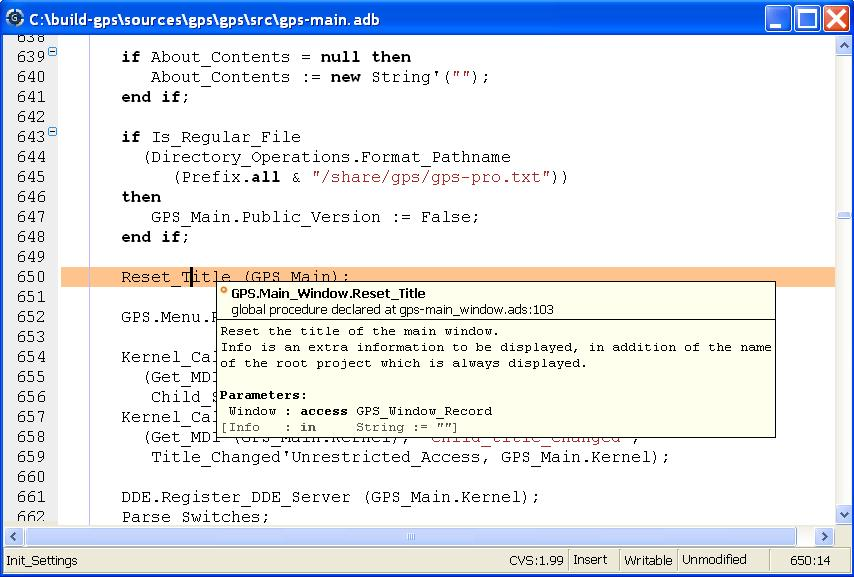
\includegraphics{source-editor.jpg}

The integrated source editor provides all the usual capabilities found in
integrated environments, including:
\begin{description}
\item[{\emph{Title bar}}] \leavevmode
Showing the full name of the file including path information.

\item[{\emph{Line number information}}] \leavevmode
This is the left area of the source editor. Line numbers can be disabled from
the preferences. {\hyperref[extending:the-preferences-dialog]{\emph{The Preferences Dialog}}}.  Note that this area can also
display additional information, such as the current line of execution when
debugging, or cvs annotations.

\item[{\emph{Scrollbar}}] \leavevmode
Located on the right of the editor, it allows you to scroll through the
source file.

\item[{\emph{Speed column}}] \leavevmode
This column, when visible, is located on the left of the editor. It allows
you to view all the highlighted lines in a file, at a glance. For example,
all the lines containing compilation errors are displayed in the Speed
Column.  See {\hyperref[extending:the-preferences-dialog]{\emph{The Preferences Dialog}}} for information on how to
customize the behavior of the Speed Column.

\item[{\emph{Status bar}}] \leavevmode
Giving information about the file. It is divided in two sections, one
on the left and one on the right of the window.

\item[{\emph{The left section}}] \leavevmode
The first box on the left shows the current subprogram name for languages
that support this capability. Currently \emph{Ada}, \emph{C} and \emph{C++} have this
ability. See {\hyperref[extending:the-preferences-dialog]{\emph{The Preferences Dialog}}} to enable or disable this feature.

\item[{\emph{The right section}}] \leavevmode
If the file is maintained under version control, and version control is
supported and enabled in GPS, the first box on the left will show VCS
information on the file: the VCS kind (e.g. \emph{CVS}), followed by the revision
number, and if available, the status of the file.

The second box shows the current editing mode. This is either \emph{Insert} or
\emph{Overwrite} and can be changed using the insert keyboard keys by default.

The third box shows the writable state of the file.  You can change this
state by clicking on the label directly: this will switch between \emph{Writable}
and \emph{Read Only}.  Note that this will not change the permissions of the file
on disk, it will only change the writable state of the source editor within
GPS.

When trying to save a file which is read only on the disk, GPS will ask for
confirmation, and if possible, will force saving of the file, keeping its
read only state.

The fourth box shows whether the file has been modified since the last save.
The three possible states are:

\item[{\emph{Unmodified}}] \leavevmode
The file has not been modified since the file has been loaded or saved.

\item[{\emph{Modified}}] \leavevmode
The file has been modified since last load or save. Note that if you undo all
the editing operations until the last save operation, this label will change
to \emph{Unmodified}.

\item[{\emph{Saved}}] \leavevmode
The file has been saved and not modified since.

The fifth box displays the position of the cursor in the file by a line and a
column number.

\item[{\emph{Contextual menu}}] \leavevmode
Displayed when you right-click on any area of the source editor.  See in
particular {\hyperref[navigation:contextual-menus-for-source-navigation]{\emph{Contextual Menus for Source Navigation}}} for more details.

\item[{\emph{Syntax highlighting}}] \leavevmode
Based on the programming language associated with the file, reserved words
and languages constructs such as comments and strings are highlighted in
different colors and fonts. See {\hyperref[extending:the-preferences-dialog]{\emph{The Preferences Dialog}}} for a list of
settings that can be customized.

By default, GPS knows about many languages. You can also easily add support
for other languages through XML files. Most languages supported by GPS will
provide syntax highlighting in the editor.

\item[{\emph{Automatic indentation}}] \leavevmode
\index{indentation}
When enabled, lines are automatically indented each time you press the
\code{Enter} key, or by pressing the indentation key.  The indentation key is
\code{Ctrl-Tab} by default, and can be changed in the key manager dialog,
{\hyperref[extending:the-key-manager-dialog]{\emph{The Key Manager Dialog}}}.

If a set of lines is selected when you press the indentation key, this whole
set of lines will be indented.

\item[{\emph{Tooltips}}] \leavevmode
\index{tooltip}
When you leave the mouse over a word in the source editor, a small window
will automatically pop up if there are relevant contextual information to
display about the word.

The type of information displayed depends on the current state of GPS.

In normal mode, the entity kind and the location of declaration is displayed
when this information is available. That is, when the cross-reference
information about the current file has been generated. If there is no
relevant information, no tooltip is displayed.  See
{\hyperref[navigation:support-for-cross-references]{\emph{Support for Cross-References}}} for more information.

In addition, the documentation for the entity is displayed. This is the block
of comments just before or just after the entity's declaration of body. There
mustn't be any blank line between the two. For instance, the following are
valid documentation for Ada and C:

\begin{Verbatim}[commandchars=\\\{\}]
\PYG{c+c1}{--  A comment for A}
\PYG{n}{A} \PYG{p}{:} \PYG{k+kt}{Integer}\PYG{p}{;}

\PYG{n}{B} \PYG{p}{:} \PYG{k+kt}{Integer}\PYG{p}{;}
\PYG{c+c1}{--  A comment for B}

\PYG{n}{C} \PYG{p}{:} \PYG{k+kt}{Integer}\PYG{p}{;}

\PYG{c+c1}{--  Not a comment for C, there is a blank linke}
\end{Verbatim}

In debugging mode, the value of the variable under the mouse is displayed in
the pop up window if the variable is known to the debugger.  Otherwise, the
normal mode information is displayed.

You can disable the automatic pop up of tool tips in the Editor section of
the preferences dialog. {\hyperref[extending:the-preferences-dialog]{\emph{The Preferences Dialog}}}.

\item[{\emph{Code completion}}] \leavevmode
\index{completion}
GPS provides two kinds of code completion: a {\hyperref[editing:smart-completion]{\emph{smart code completion}}} based on semantic information, and a text completion.

It is useful when editing a file and using often the same words to get
automatic word completion. This is possible by typing the \code{Ctrl-/} key
combination (customizable through the key manager dialog) after a partial
word: the next possible completion will be inserted in the editor. Typing
this key again will cycle through the list of possible completions.

Text completions are searched in all currently open source files, by first
looking at the closest words and then looking further in the source as
needed.

\item[{\emph{Delimiter highlighting}}] \leavevmode
\index{delimiter}
When the cursor is moved before an opening delimiter or after a closing
delimiter, then both delimiters will be highlighted. The following characters
are considered delimiters: (){[}{]}\{\}.  You can disable highlighting of
delimiters in the preferences.

You can also jump to a corresponding delimiter by using the \code{Ctrl-'}
key, that can be configured in the preferences. Typing twice on this key will
move the cursor back to its original position.

\item[{\emph{Current line highlighting}}] \leavevmode
\index{current line}
You can configure the editor to highlight the current line with a certain
color. {\hyperref[extending:the-preferences-dialog]{\emph{The Preferences Dialog}}}.

\item[{\emph{Current block highlighting}}] \leavevmode
\index{block}
If this preference is enabled, the editor will highlight the current block of
code, e.g. the current \emph{begin...end} block, or loop statement, etc...

The block highlighting will also take into account the changes made in your
source code, and will recompute automatically the current block when needed.

This capability is currently implemented for Ada, C and C++ languages.

\item[{\emph{Block folding}}] \leavevmode
\index{block}
When enabled, the editor will display \emph{-} icons on the left side,
corresponding to the beginning of subprograms. If you click on one of these
icons, all the lines corresponding to this subprogram are hidden, except the
first one. As for the block highlighting, these icons are recomputed
automatically when you modify your sources and are always kept up to date.

This capability is currently implemented for Ada, C and C++ languages.

\item[{\emph{Auto save}}] \leavevmode
\index{auto save}
You can configure the editor to periodically save modified files.  See
{\hyperref[extending:autosave-delay]{\emph{Autosave delay}}} for a full description of this
capability.

\item[{\emph{Automatic highlighting of entities}}] \leavevmode
\index{auto highlighting}
When the cursor is positioned on an entity in the source editor, GPS will
highlight all references to this entity in the current editor.

When the cursor moves away from the entity, the highlighting is removed.

This is controlled by the plugin \emph{auto\_highlight\_occurrences.py}: it can be
deactivated by deactivating the plugin ({\hyperref[extending:the-plug-ins-editor]{\emph{The Plug-ins Editor}}}).

Details such as presence of indications in the Speed Column or highlighting
color can be customized in the \emph{Plugins} section of
{\hyperref[extending:the-preferences-dialog]{\emph{The Preferences Dialog}}}.

\end{description}

\index{emacs}
GPS also integrates with existing third party editors such as \emph{Emacs} or \emph{vi}.
{\hyperref[editing:using-an-external-editor]{\emph{Using an External Editor}}}.


\section{Editing Sources}
\label{editing:editing-sources}\label{editing:id3}
\index{editing}
\index{source file}

\subsection{Key bindings}
\label{editing:key-bindings}\label{editing:index-13}
\index{key}
In addition to the standard keys used to navigate in the editor (up, down,
right, left, page up, page down), the integrated editor provides a number of
key bindings allowing easy navigation in the file.

There are also several ways to define new key bindings, see
{\hyperref[extending:defining-text-aliases]{\emph{Defining text aliases}}} and {\hyperref[extending:binding-actions-to-keys]{\emph{Binding actions to keys}}}.
\begin{description}
\item[{\emph{Ctrl-Shift-u}}] \leavevmode
\index{hexadecimal}
\index{ASCII}
Pressing these three keys and then holding Ctrl-Shift allow you to enter
characters using their hexadecimal value. For example, pressing
\code{Ctrl-Shift-u-2-0} will insert a space character (ASCII 32, which is 20
in hexadecimal).

\item[{\emph{Ctrl-x / Shift-delete}}] \leavevmode
Cut to clipboard

\item[{\emph{Ctrl-c / Ctrl-insert}}] \leavevmode
Copy to clipboard

\item[{\emph{Ctrl-v / Shift-insert}}] \leavevmode
Paste from clipboard

\item[{\emph{Ctrl-s}}] \leavevmode
Save file to disk

\item[{\emph{Ctrl-z}}] \leavevmode
Undo previous insertion/deletion

\item[{\emph{Ctrl-r}}] \leavevmode
Redo previous insertion/deletion

\item[{\emph{Insert}}] \leavevmode
Toggle overwrite mode

\item[{\emph{Ctrl-a}}] \leavevmode
Select the whole file

\item[{\emph{Home / Ctrl-Pgup}}] \leavevmode
Go to the beginning of the line

\item[{\emph{End / Ctrl-Pgdown}}] \leavevmode
Go to the end of the line

\item[{\emph{Ctrl-Home}}] \leavevmode
Go to the beginning of the file

\item[{\emph{Ctrl-End}}] \leavevmode
Go to the end of the file

\item[{\emph{Ctrl-up}}] \leavevmode
Go to the beginning of the line, or to the previous line if already at the
beginning of the line.

\item[{\emph{Ctrl-down}}] \leavevmode
Go to the end of the line, or to the beginning of the next line if already at
the end of the line.

\item[{\emph{Ctrl-delete}}] \leavevmode
Delete end of the current word.

\item[{\emph{Ctrl-backspace}}] \leavevmode
Delete beginning of the current word.

\end{description}


\section{The File Selector}
\label{editing:id4}\label{editing:the-file-selector}
\index{file selector}
\index{Windows}
The file selector is a dialog used to select a file. Under Windows, the default
is to use the standard file selection widget. Under other platforms, the file
selector is a built-in dialog:

\index{screen shot}
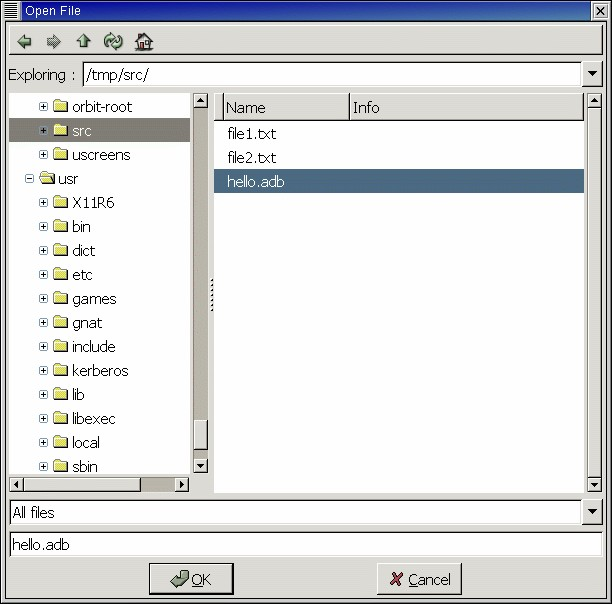
\includegraphics{open-file.jpg}

This dialog provides the following areas and capabilities:
\begin{itemize}
\item {} 
A tool bar on the top composed of five buttons giving access to common
navigation features:

\item {} 
\code{left arrow}
go back in the list of directories visited

\item {} 
\code{right arrow}
go forward

\item {} 
\code{up arrow}
go to parent directory

\item {} 
\code{refresh}
refresh the contents of the directory

\item {} 
\code{home}
go to home directory (value of the HOME environment variable, or \emph{/} if
not defined)

\item {} 
A list with the current directory and the last directories explored.
You can modify the current directory by modifying the text entry and hitting
\code{Enter}, or by clicking on the right arrow and choose a previous
directory in the pop down list displayed.

\item {} 
A directory tree. You can open or close directories by clicking on the \emph{+}
and \emph{-} icons on the left of the directories, or navigate using the keyboard
keys: \code{up} and \code{down} to select the previous or the next directory,
\code{+} and \code{-} to expand and collapse the current directory, and
\code{backspace} to select the parent directory.

\item {} 
A file list. This area lists the files contained in the selected directory.
If a filter is selected in the filter area, only the relevant files for the
given filter are displayed. Depending on the context, the list of files may
include additional information about the files, e.g. the kind of a file, its
size, etc...

\item {} 
A filter area. Depending on the context, one or several filters are available
to select only a subset of files to display. The filter \emph{All files} which is
always available will display all files in the directory selected.

\item {} 
A file name area. This area will display the name of the current file
selected, if any.  You can also type a file or directory name directly, and
complete the name automatically by using the \code{Tab} key.

\item {} 
A button bar with the \emph{OK} and \emph{Cancel} buttons.  When you have selected the
right file, clock on \emph{OK} to confirm, or click on \emph{Cancel} at any time to
cancel and close the file selection.

\end{itemize}


\section{Menu Items}
\label{editing:id5}\label{editing:menu-items}
\index{menu}
The main menus that give access to extended functionalities related to source
editing are described in this section.


\subsection{The File Menu}
\label{editing:id6}\label{editing:the-file-menu}\begin{description}
\item[{\emph{New}}] \leavevmode
\index{new file}
Open a new untitled source editor.  No syntax highlighting is performed until
the file is saved, since GPS needs to know the file name in order to choose
the programming language associated with a file.

\index{Ada}
When you save a new file for the first time, GPS will ask you to enter the
name of the file. In case you have started typing Ada code, GPS will try to
guess based on the first main entity in the editor and on the current naming
scheme, what should be the default name of this new file.

\item[{\emph{New View}}] \leavevmode
\index{new view}
\index{view}
Create a new view of the current editor. The new view shares the same
contents: if you modify one of the source views, the other view is updated at
the same time. This is particularly useful when you want to display two
separate parts of the same file, for example a function spec and its body.

A new view can also be created by keeping the \code{shift} key pressed while
drag-and-dropping the editor (see {\hyperref[mdi:moving-windows]{\emph{Moving Windows}}}). This second method
is preferred, since you can then specify directly where you want to put the
new view. The default when using the menu is that the new view is put on top
of the editor itself.

\item[{\emph{Open...}}] \leavevmode
\index{open}
\index{Windows}
Open a file selection dialog where you can select a file to edit.  Under
Windows, this is the standard file selector. Under other platforms, this is a
built-in file selector described in {\hyperref[editing:the-file-selector]{\emph{The File Selector}}}.

\item[{\emph{Open From Project...}}] \leavevmode\phantomsection\label{editing:open-from-project}
\index{open}
\index{project}
Open a dialog where you can easily and rapidly select a source file from your
project.

\index{screen shot}
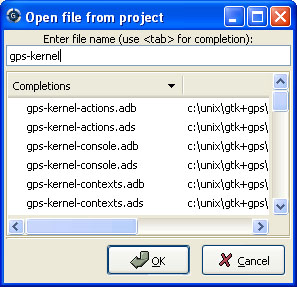
\includegraphics{open-from-project.jpg}

The first text area allows you to type a file name. You can start the
beginning of a file name, and use the \code{Tab} key to complete the file
name. If there are several possible completions, the common prefix will be
displayed, and a list of all possible completions will be displayed in the
second text area.

\index{key}
You can then either complete the name by typing it, or continue hitting the
\code{Tab} key to cycle through the possible completions, or click on one of
the completions in the list displayed.

If you press the down arrow key, the focus will move to the list of
completions, so that you can select a file from this list without using the
mouse.

Once you have made your choice, click on the \emph{OK} button to validate.
Clicking on \emph{Cancel} or hitting the \code{Esc} key will cancel the operation
and close the dialog.

This dialog will only show each file once. If you have extended projects in
your hierarchy, some files may be redefined in some extending project. In
this case, only the files from the extending project are shown, and you
cannot have access through this dialog to the overridden files of the
extended project. Of course, you can still use the project view or the
standard \emph{File-\textgreater{}Open} menu to open these files.

\item[{\emph{Open From Host...}}] \leavevmode\phantomsection\label{editing:open-from-host}
\index{open}
Open a file selector dialog where you can specify a remote host, as defined
in {\hyperref[remote:the-remote-configuration-dialog]{\emph{The remote configuration dialog}}}. You have access to a remote host
file system, can specify a file which can be edited in GPS. When you hit the
save button or menu, the file will be saved on the remote host.

See also {\hyperref[remote:using-gps-for-remote-development]{\emph{Using GPS for Remote Development}}} for a more efficient way to
work locally on remote files.

\item[{\emph{Recent}}] \leavevmode
\index{recent}
Open a sub menu containing a list of the ten most recent files opened in GPS,
so that you can reopen them easily.

\item[{\emph{Save}}] \leavevmode
\index{save}
Save the current source editor if needed.

\item[{\emph{Save As...}}] \leavevmode
\index{save as}
Same current file under a different name, using the file selector dialog.
{\hyperref[editing:the-file-selector]{\emph{The File Selector}}}.

\item[{\emph{Save More}}] \leavevmode
\index{save}
Give access to extra save capabilities.

\item[{\emph{All}}] \leavevmode
\index{save all}
Save all items, including projects, etc...

\item[{\emph{Desktop}}] \leavevmode
\index{save desktop}
Save the desktop to a file. The desktop includes information about files,
graphs, ... and their window size and position in GPS. The desktop is saved
per top level project, so that if you reload the same project you get back to
the same situation you were in when you left GPS. Instead, if you load a
different project another desktop will be loaded (or the default desktop).
Through the preference ``Save Desktop On Exit'', you can also automatically
save this desktop when you quit GPS.

\item[{\emph{Change Directory...}}] \leavevmode
\index{directory}
Open a directory selection dialog that lets you change the current working
directory.

\item[{\emph{Messages}}] \leavevmode
\index{messages}
This sub menu gives access to functionalities related to the Messages window.
{\hyperref[main_window:the-messages-window]{\emph{The Messages Window}}}.

\item[{\emph{Clear}}] \leavevmode
\index{messages}
\index{clear}
Clear the contents of the Messages window.

\item[{\emph{Save As...}}] \leavevmode
\index{save as}
Save the contents of the Messages window to a file. A file selector is
displayed to choose the name and location of the file.

\item[{\emph{Load Contents...}}] \leavevmode
\index{load}
Open a file selector to load the contents of a file in the Messages window.
Source locations are identified and loaded in {\hyperref[main_window:the-locations-view]{\emph{The Locations View}}}.

\item[{\emph{Export Locations to Editor}}] \leavevmode
\index{export locations}
List the contents of the Locations view in a standard text editor.

\item[{\emph{Close}}] \leavevmode
\index{close}
Close the current window. This applies to all GPS windows, not only source
editors.

\item[{\emph{Print}}] \leavevmode
\index{print}
Print the current window contents, optionally saving it interactively if it
has been modified. The Print Command specified in the preferences is used if
it is defined. On Unix this command is required; on Windows it is optional.

On Windows, if no command is specified in the preferences the standard
Windows print dialog box is displayed. This dialog box allows the user to
specify the target printer, the properties of the printer, which pages to
print (all, or a specific range of pages), the number of copies to print,
and, when more than one copy is specified, whether the pages should be
collated.  Pressing the Cancel button on the dialog box returns to GPS
without printing the window contents; otherwise the specified pages and
copies are printed on the selected printer. Each page is printed with a
header containing the name of the file (if the window has ever been saved).
The page number is printed on the bottom of each page.

See also:ref:\emph{Print Command \textless{}Print\_Command\textgreater{}}.

\item[{\emph{Exit}}] \leavevmode
\index{exit}
\index{quit}
Exit GPS after confirmation and if needed, confirmation about saving modified
windows and editors.

\end{description}


\subsection{The Edit Menu}
\label{editing:id7}\label{editing:the-edit-menu}
\index{menu}
\index{edit}\begin{description}
\item[{\emph{Undo}}] \leavevmode
\index{undo}
Undo previous insertion/deletion in the current editor.

\item[{\emph{Redo}}] \leavevmode
\index{redo}
Redo previous insertion/deletion in the current editor.

\item[{\emph{Cut}}] \leavevmode
\index{cut}
Cut the current selection and store it in the clipboard.

\item[{\emph{Copy}}] \leavevmode
\index{copy}
\index{yank}
Copy the current selection to the clipboard.

\item[{\emph{Paste}}] \leavevmode
\index{paste}
Paste the contents of the clipboard to the current cursor position.

\item[{\emph{Paste Previous}}] \leavevmode
\index{paste previous}
GPS stores a list of all the text that was previously copied into the
clipboard through the use of Copy or Cut.

By default, if you press Paste, the newest text will be copied at the current
position. But if you select Paste Previous immediately after (one or more
times) you can instead paste text that was copied previously in the
clipboard.

For instance, if you copy through \emph{Edit-\textgreater{}Copy} the text ``First'', then copy
the text ``Second'', you can then select \emph{Edit-\textgreater{}Paste} to insert ``Second'' at
the current location. If you then select \emph{Edit-\textgreater{}Paste Previous}, ``Second''
will be replaced by ``First''.

Selecting this menu several times will replace the text previously pasted by
the previous one in the list saved in the clipboard. When reaching the end of
this list, GPS will started from the beginning, and insert again the last
text copied into the clipboard.

The size of this list is controlled by the \emph{Clipboard Size} preference.

For more information, {\hyperref[main_window:the-clipboard-view]{\emph{The Clipboard View}}}.

\item[{\emph{Select All}}] \leavevmode
\index{select all}
Select the whole contents of the current source editor.

\item[{\emph{Rectangles...}}] \leavevmode
See the section {\hyperref[editing:rectangles]{\emph{Rectangles}}} for more information on rectangles.

\item[{\emph{Insert File...}}] \leavevmode
Open a file selection dialog and insert the contents of this file in the
current source editor, at the current cursor location.

\item[{\emph{Insert Shell Output...}}] \leavevmode
Open an input window at the bottom of the GPS window where you can specify
any external command. The output of the command will be inserted at the
current editor location in case of success. If text is selected, the text is
passed to the external command and replaced by the command's output.

\item[{\emph{Format Selection}}] \leavevmode
\index{format selection}
Indent and format the selection or the current line.
{\hyperref[extending:the-preferences-dialog]{\emph{The Preferences Dialog}}}, for preferences related to source formatting.

\end{description}

\emph{Smart Completion}
\begin{quote}
\phantomsection\label{editing:smart-completion}
\index{completion}
Complete the identifier prefix under the cursor, and list the results in a
pop-up list. Used with Ada sources this command can take advantage of an
entity database as well as Ada parsers embedded in GPS which analyze the
context, and offer completions from the entire project along with
documentation extracted from comments surrounding declarations. To take full
advantage of this feature, the smart completion preference must be enabled,
which will imply the computation of the entity database at GPS startup.

The support for C and C++ is not as powerful as the support for Ada since it
relies completely on the xref information files generated by the compiler,
does not have into account the C/C++ context around the cursor, and does not
extract documentation from comments around candidate declarations. To take
advantage of this feature, in addition to enable the smart completion
preference, the C/C++ application must be built with \emph{-fdump-xref}.

In order to use this feature, open any Ada, C or C++ file, and begin to type
an identifier. It has to be an identifier declared either in the current file
(and accessible from the cursor location) or in one of the packages of the
project loaded. Move the cursor right after the last character of the
incomplete identifier and hit the completion key (which is \code{ctrl+space}
by default).  GPS will open a popup displaying all the known identifiers
beginning with the prefix you typed. You can then browse among the various
proposals by clicking on the  \code{up} and \code{down} keys, or using the
left scrollbar. For each entity, a documentation box is filled. If the
location of the entity is known, it's displayed as an hyperlink, and you can
jump directly to its declaration by clicking on it.

Typing new letters will reduce the range of proposal, as long as there remain
solutions. Once you've selected the expected completion, you can validate by
pressing \code{Enter}.

Typing control characters (ie, characters which cannot be used in
identifiers) will also validate the current selection.

GPS is also able to complete automatically subprogram parameter or dotted
notations. For example, if you type:

\begin{Verbatim}[commandchars=\\\{\}]
\PYG{k+kn}{with} \PYG{n+nn}{Ada.}
\end{Verbatim}

the smart completion window will appear automatically, listing all the child
and nested packages of Ada. You can configure the time interval after which
the completion window appears ({\hyperref[extending:the-preferences-dialog]{\emph{The Preferences Dialog}}}).

You can also write the beginning of the package, e.g.:

\begin{Verbatim}[commandchars=\\\{\}]
\PYG{k+kn}{with} \PYG{n+nn}{Ada.Text}
\end{Verbatim}

pressing the completion key will offer you Text\_IO.

If you are in a code section, you will be able to complete the fields of a
record, or the contents of a package, e.g.:

\begin{Verbatim}[commandchars=\\\{\}]
 \PYG{k+kr}{declare}
   \PYG{k+kd}{type} \PYG{k+kt}{R} \PYG{k+kr}{is} \PYG{k+kr}{record}
      \PYG{n+nv}{Field1} \PYG{p}{: }\PYG{n+nv}{Integer}\PYG{p}{;}
      \PYG{n+nv}{Field2} \PYG{p}{: }\PYG{n+nv}{Integer}\PYG{p}{;}
   \PYG{n+nv}{end} \PYG{n+nv}{record}\PYG{p}{;}

   \PYG{n+nv}{V} \PYG{p}{: }\PYG{n+nv}{R}\PYG{p}{;}
\PYG{n+nv}{begin}
   \PYG{n+nv}{V}\PYG{p}{.}
\end{Verbatim}

Completing V. will propose Field1 and Field2.

The smart completion can also give you the possible parameters of a call
you're currently making. For example, in the following code:

\begin{Verbatim}[commandchars=\\\{\}]
   \PYG{k+kd}{procedure} \PYG{n+nf}{Proc} \PYG{p}{(}\PYG{n+nv}{A}\PYG{p}{,} \PYG{n+nv}{B}\PYG{p}{,} \PYG{n+nv}{C} \PYG{p}{: }\PYG{n+nv}{Integer}\PYG{p}{)}\PYG{p}{;}
\PYG{k+kr}{begin}
   \PYG{n}{Proc} \PYG{p}{(}\PYG{l+m+mi}{1}\PYG{p}{,}
\end{Verbatim}

If you hit the completion key after the comma, the smart completion engine
will propose you to complete with the named parameters ``B =\textgreater{}'', ``C =\textgreater{}'' or
directly to complete with all the remaining parameters, which in this case
will be ``B =\textgreater{}, C =\textgreater{} )''.

\index{screen shot}
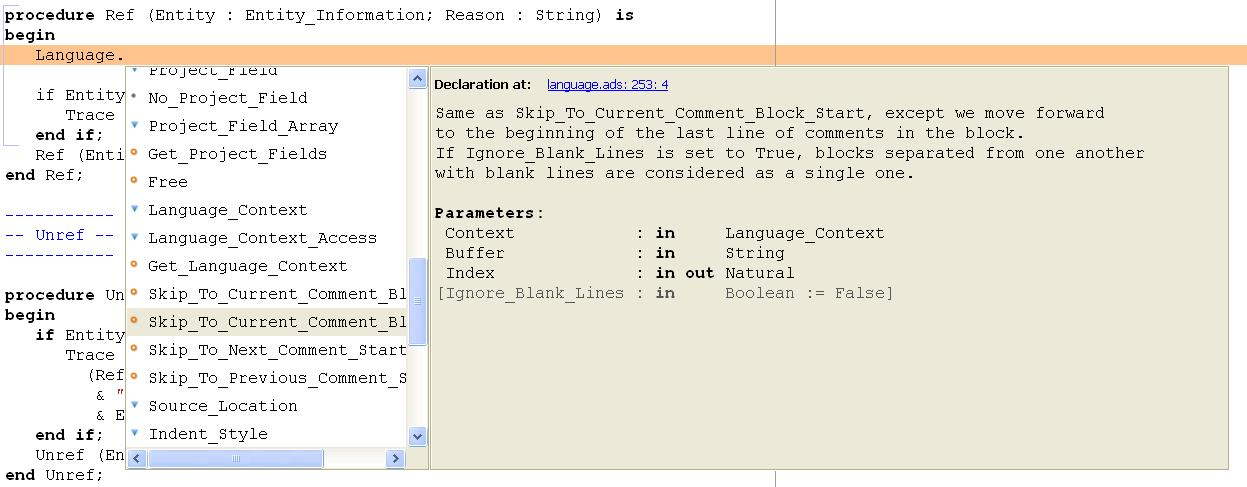
\includegraphics{smart-completion.jpg}

Limitations:
\end{quote}
\begin{itemize}
\item {} 
This feature is currently only available for Ada, C and C++. Using the smart
completion on sources of other languages behaves as the {\hyperref[editing:complete-identifier]{\emph{identifier
completion}}} does.

\item {} 
Smart completion for C and C++ is based on the xref information generated by
the compiler. Therefore, GPS has no knowledge on recently edited files. Use
Build-\textgreater{}Recompute Xref Info or rebuild with \emph{-fdump-xref} to update the
completion database.

\item {} 
Smart completion for C and C++ is only triggered at the beginning of an
expression (that is, it is not triggered on special characters such as `(`,
`-\textgreater{}', or the C++ operator `::') and it may propose too much candidates since
it does not have into account the C/C++ syntax context. Typing new letters
will reduce the range of proposal, as long as there remain solutions.

\item {} 
Smart completion of subprogram parameters, fields and dotted notation are not
available yet for C and C++.

\item {} 
\emph{More Completion}
.. index:: completion

This submenu contains more ways to automatically complete code
\begin{itemize}
\item {} 
\emph{Expand Alias}
Consider the current word as an alias and expand according to aliases
defined in {\hyperref[extending:defining-text-aliases]{\emph{Defining text aliases}}}.

\item {} 
\emph{Complete Identifier}
\phantomsection\label{editing:complete-identifier}
\index{complete identifier}
Complete the identifier prefix under the cursor. This command will cycle
through all identifiers starting with the given prefix.

\item {} 
\emph{Complete Block}
.. index:: complete block

Close the current statement (if, case, loop) or unit (procedure,
function, package). This action works only on an Ada buffer.

\end{itemize}

\end{itemize}
\begin{description}
\item[{\emph{Selection}}] \leavevmode
\index{selection}\begin{description}
\item[{\emph{Comment Lines}}] \leavevmode
\index{comment}
Comment the current selection or line based on the current programming
language syntax.

\item[{\emph{Uncomment Lines}}] \leavevmode
\index{uncomment}
Remove the comment delimiters from the current selection or line.

\item[{\emph{Refill}}] \leavevmode
\index{refill}
Refill text on the selection or current line: rearrange line breaks in
the paragraph so that line lengths do not exceed the maximum length, as
set in the ``Right margin'' preference ({\hyperref[extending:the-preferences-dialog]{\emph{The Preferences Dialog}}}).

\item[{\emph{Sort}}] \leavevmode
Sort the selected lines alphabetically. This is particularly useful when
editing non source code, or for specific parts of the code, like with
clauses in Ada.

\item[{\emph{Sort Reverse}}] \leavevmode
Sort the selected lines in reverse alphabetical order

\item[{\emph{Pipe in external program...}}] \leavevmode
Open an input window at the bottom of the GPS window where you can
specify any external command, which will take the current selection as
input. The output of the command will replace the contents of the
selection on success.

\item[{\emph{Serialize}}] \leavevmode
Increment a set of numbers found on adjacent lines.  The exact behavior
depends on whether there is a current selection or not.

If there is no selection, then the set of lines considered is from the
current line on and includes all adjacent lines that have at least one
digit in the original columns. In the following example, `\textbar{}' marks the
place where the cursor is at the beginning:

\begin{Verbatim}[commandchars=\\\{\}]
\PYG{n}{AAA} \PYG{p}{\textbar{}}\PYG{l+m+mi}{10} \PYG{n}{AAA}
\PYG{n}{CCC} \PYG{l+m+mi}{34567} \PYG{n}{CCC}
\PYG{n}{DDD} \PYG{n}{DDD}
\end{Verbatim}

then only the first two lines will be modified, and will become:

\begin{Verbatim}[commandchars=\\\{\}]
\PYG{n}{AAA} \PYG{l+m+mi}{10} \PYG{n}{AAA}
\PYG{n}{CCC} \PYG{l+m+mi}{11} \PYG{n}{CCC}
\PYG{n}{DDD} \PYG{n}{DDD}
\end{Verbatim}

If there is a selection, all the lines in the selection are
modified. For each line, the columns that had digits in the first
line are modified, no matter what they actually contain. In the
example above, if you select all three lines, the replacement becomes:

\begin{Verbatim}[commandchars=\\\{\}]
\PYG{n}{AAA} \PYG{l+m+mi}{10} \PYG{n}{AAA}
\PYG{n}{CCC} \PYG{l+m+mi}{11567} \PYG{n}{CCC}
\PYG{n}{DDD} \PYG{l+m+mi}{12}\PYG{n}{D}
\end{Verbatim}

ie only the fifth and sixth columns are modified since only those
columns contained digits in the first line. This feature assumes that
you are selecting a relevant set of lines. But it allows you to
transform blank lines more easily. For instance, if you have:

\begin{Verbatim}[commandchars=\\\{\}]
\PYG{n}{AAA} \PYG{l+m+mi}{1}
\PYG{n}{BBB}
\PYG{n}{CCC}
\end{Verbatim}

this is transformed into:

\begin{Verbatim}[commandchars=\\\{\}]
\PYG{n}{AAA} \PYG{l+m+mi}{1}
\PYG{n}{BBB} \PYG{l+m+mi}{2}
\PYG{n}{CCC} \PYG{l+m+mi}{3}
\end{Verbatim}

\item[{\emph{Untabify}}] \leavevmode
Replace all tabs in the current selection (or in the whole buffer if
there is no selection) by the appropriate number of spaces

\item[{\emph{Move Right} and \emph{Move Left}}] \leavevmode
Shift the currently selected lines (or the current line if there is no
selection) one character to the right or to the left

\end{description}

\item[{\emph{Fold all blocks}}] \leavevmode
\index{fold}
Collapse all the blocks in the current file.

\item[{\emph{Unfold all blocks}}] \leavevmode
\index{unfold}
Uncollapse all the blocks in the current file.

\item[{\emph{Create Bookmark}}] \leavevmode
Creates a new Bookmark at cursor position. For more information,
{\hyperref[main_window:bookmarks]{\emph{Bookmarks}}}.

\item[{\emph{Pretty Print}}] \leavevmode
\index{gnatpp}
\index{pretty print}
Pretty print the current source editor by calling the external tool \emph{gnatpp}.
It is possible to specify \emph{gnatpp} switches in the switch editor.
{\hyperref[projects:the-switches-editor]{\emph{The Switches Editor}}}.

\item[{\emph{Generate Body}}] \leavevmode
\index{gnatstub}
\index{generate body}
Generate Ada body stub for the current source editor by calling the external
tool \emph{gnatstub}.

\item[{\emph{Edit with external editor}}] \leavevmode
{\hyperref[editing:using-an-external-editor]{\emph{Using an External Editor}}}.

\item[{\emph{Aliases}}] \leavevmode
\index{alias}
Display the Aliases editor. {\hyperref[extending:defining-text-aliases]{\emph{Defining text aliases}}}.

\item[{\emph{Key shortcuts}}] \leavevmode
\index{key shortcuts}
Give access to the key manager dialog, to associate commands with special
keys. {\hyperref[extending:the-key-manager-dialog]{\emph{The Key Manager Dialog}}}.

\item[{\emph{Preferences}}] \leavevmode
\index{preferences}
Give access to the preferences dialog. {\hyperref[extending:the-preferences-dialog]{\emph{The Preferences Dialog}}}.

\end{description}


\section{Rectangles}
\label{editing:rectangles}\label{editing:id8}
\index{rectangle}
Rectangle commands operate on a rectangular area of the text, that is all the
characters between two columns in a certain range of lines.

A rectangle is selected using the standard selection mechanism. You can
therefore use either the mouse to highlight the proper region, or \code{shift}
and the cursor keys to extend the selection, or the Emacs selection (with the
mark and the current cursor location) if you have activated the
\code{emacs.py} plugin.

Visually, a selected rectangle is exactly the same as the standard selection.
In particular, the characters after the last column, on each line, will also be
highlighted. The way the selection is interpreted (either as a full text or as
a rectangle) depends on the command you then chose to manipulate the selection.

If you chose one of the commands from the \emph{/Edit/Rectangles} menu, the actual
rectangle will extend from the top-left corner down to the bottom-right corner.
All characters to the right of the right-most column, although they are
highlighted, are not part of the rectangle.

Consider for instance the following initial text:

\begin{Verbatim}[commandchars=\\\{\}]
\PYG{k+kd}{package} \PYG{n+nc}{A} \PYG{k+kr}{is}
   \PYG{k+kd}{procedure} \PYG{n+nf}{P}\PYG{p}{;}

   \PYG{k+kd}{procedure} \PYG{n+nf}{Q}\PYG{p}{;}
\PYG{k+kr}{end} \PYG{n+nf}{A}\PYG{p}{;}
\end{Verbatim}

and assume we have selected from the character ``p'' in ``procedure P'', down to
the character ``c'' in ``procedure Q''.

The following commands can then be used (either from the menu, or you can
assign key shortcuts to them via the usual \emph{/Edit/Key shortcuts} menu.
\begin{itemize}
\item {} 
\emph{Cut} or \emph{Delete}
These commands will remove the selected text (and have no effect on empty
lines within the rectangle). The former will in addition copy the rectangle
to the clipboard, so that you can paste it later. In our example, we end up
with:

\begin{Verbatim}[commandchars=\\\{\}]
\PYG{k+kd}{package} \PYG{n+nc}{A} \PYG{k+kr}{is}
   \PYG{n}{edure} \PYG{n}{P}\PYG{p}{;}

   \PYG{n}{edure} \PYG{n}{Q}\PYG{p}{;}
\PYG{k+kr}{end} \PYG{n+nf}{A}\PYG{p}{;}
\end{Verbatim}

\item {} 
\emph{Copy}
This command has no visual effect, but copies the contents of the rectangle
into the clipboard.

\item {} 
\emph{Paste}
Pastes the contents of the clipboard as a rectangle: each line from the
clipboard is treated independently, and inserted on successive lines in the
current editor. They all start in the same column (the one where the cursor
is initially in), and existing text in the editor lines is shifted to the
right). If for instance you now place the cursor in the second line, first
column, and paste, we end up with:

\begin{Verbatim}[commandchars=\\\{\}]
\PYG{k+kd}{package} \PYG{n+nc}{A} \PYG{k+kr}{is}
\PYG{n}{proc}   \PYG{n}{edure} \PYG{n}{P}\PYG{p}{;}

\PYG{n}{proc}   \PYG{n}{edure} \PYG{n}{Q}\PYG{p}{;}
\PYG{k+kr}{end} \PYG{n+nf}{A}\PYG{p}{;}
\end{Verbatim}

\item {} 
\emph{Clear}
Replaces the contents of the selected rectangle with spaces. If we start
from our initial exmaple, we end up with the following. Note the difference
with \emph{Delete}:

\begin{Verbatim}[commandchars=\\\{\}]
\PYG{k+kd}{package} \PYG{n+nc}{A} \PYG{k+kr}{is}
       \PYG{n}{edure} \PYG{n}{P}\PYG{p}{;}

       \PYG{n}{edure} \PYG{n}{Q}\PYG{p}{;}
\PYG{k+kr}{end} \PYG{n+nf}{A}\PYG{p}{;}
\end{Verbatim}

\item {} 
\emph{Open}
Replaces the contents of the selected rectangle with spaces, but shifts the
lines to the right to do so. Note the difference with \emph{Clear}:

\begin{Verbatim}[commandchars=\\\{\}]
\PYG{k+kd}{package} \PYG{n+nc}{A} \PYG{k+kr}{is}
       \PYG{k+kd}{procedure} \PYG{n+nf}{P}\PYG{p}{;}

       \PYG{k+kd}{procedure} \PYG{n+nf}{Q}\PYG{p}{;}
\PYG{k+kr}{end} \PYG{n+nf}{A}\PYG{p}{;}
\end{Verbatim}

\item {} 
\emph{Replace With Text}
This is similar to \emph{Clear}, but the rectangle is replaced with user-defined
text. The lines will be shifted left or right if the text you insert is
shorter (resp. longer) than the width of the rectangle. If for instance we
replace our initial rectangle with the text TMP, we end up with the
following. Note that the character ``c'' has disappeared, since TMP is shorter
than our rectangle width (4 characters). This command will impact lines that
are empty in the initial rectangle:

\begin{Verbatim}[commandchars=\\\{\}]
\PYG{k+kd}{package} \PYG{n+nc}{A} \PYG{k+kr}{is}
   \PYG{n}{TMPedure} \PYG{n}{P}\PYG{p}{;}
   \PYG{n}{TMP}
   \PYG{n}{TMPedure} \PYG{n}{Q}\PYG{p}{;}
\PYG{k+kr}{end} \PYG{n+nf}{A}\PYG{p}{;}
\end{Verbatim}

\item {} 
\emph{Insert Text}
This inserts a text to the left of the rectangle on each line. The following
example inserts TMP. Note the difference with \emph{Replace With Text}. This
command will also insert the text on lines that are empty in the initial
rectangle:

\begin{Verbatim}[commandchars=\\\{\}]
\PYG{k+kd}{package} \PYG{n+nc}{A} \PYG{k+kr}{is}
   \PYG{n}{TMPprocedure} \PYG{n}{P}\PYG{p}{;}
   \PYG{n}{TMP}
   \PYG{n}{TMPprocedure} \PYG{n}{Q}\PYG{p}{;}
\PYG{k+kr}{end} \PYG{n+nf}{A}\PYG{p}{;}
\end{Verbatim}

\item {} 
\emph{Sort}
This sorts the selected lines according to the key which starts and ends on
the corresponding rectangle's columns:

\begin{Verbatim}[commandchars=\\\{\}]
\PYG{n}{aaa} \PYG{l+m+mi}{15} \PYG{n}{aa}
\PYG{n}{bbb} \PYG{l+m+mi}{02} \PYG{n}{bb}
\PYG{n}{ccc} \PYG{l+m+mi}{09} \PYG{n}{cc}
\end{Verbatim}

With a selection starting from the 1 on the first line and ending on the 9 on
the last one, sorting will result with the following content:

\begin{Verbatim}[commandchars=\\\{\}]
\PYG{n}{bbb} \PYG{l+m+mi}{02} \PYG{n}{bb}
\PYG{n}{ccc} \PYG{l+m+mi}{09} \PYG{n}{cc}
\PYG{n}{aaa} \PYG{l+m+mi}{15} \PYG{n}{aa}
\end{Verbatim}

\item {} 
\emph{Sort reverse}

As above but in the reverse order.

\end{itemize}


\section{Recording and replaying macros}
\label{editing:recording-and-replaying-macros}\label{editing:id9}
\index{macros}
It is often convenient to be able to repeat a given key sequence a number of
times.

GPS supports this with several different methods:
\begin{itemize}
\item {} 
Repeat the next action

If there is a single key press that you wish to repeat a number of times, you
should first use the GPS action \emph{``Repeat Next''} (bound by default to
\code{control-u}, but this can be changed as usual through the \emph{/Edit/Key
Shortcuts} menu), then entering the number of times you wish to repeat, and
finally pressing the key you want.

For instance, the following sequence \code{control-u 79 -} will insert
79 characters `-` in the current editor. This proves often useful to insert
separators.

If you are using the emacs mode (see \emph{/Tools/Plug-ins} menu), you can also
use the sequence \code{control-u 30 control-k} to delete
30 lines.

\item {} 
Recording macros

If you wish to repeat a sequence of more than 1 key, you should record this
sequence as a macro. All macro-related menus are found in \emph{/Tools/Macros},
although it is often more convenient to use these through key bindings, which
you can of course override.

You must indicate to GPS that it should start recording the keys you are
pressing. This is done through the \emph{/Tools/Macros/Start Keyboard Macro} menu.
As its name indicates, this only records keyboard events, not mouse events.
Until you select \emph{/Tools/Macros/Stop Macro}, GPS will keep recording the
events.

In Emacs mode, the macro actions are bound to \code{control-x (},
\code{control-x )} and \code{control-x e} key shortcuts. For instance, you
can execute the following to create a very simple macro that deletes the
current line, wherever your cursor initially is on that line:
\begin{itemize}
\item {} 
\code{control-x (}     start recording

\item {} 
\code{control-a}      go to beginning of line

\item {} 
\code{control-k}      delete line

\item {} 
\code{control-x )}     stop recording

\end{itemize}

\end{itemize}


\section{Contextual Menus for Editing Files}
\label{editing:id10}\label{editing:contextual-menus-for-editing-files}
\index{case exceptions}
Whenever you ask for a contextual menu (using e.g. the third button on your
mouse) on a source file, you will get access to a number of entries, displayed
or not depending on the current context.

Menu entries include the following categories:
\begin{description}
\item[{\emph{Source Navigation}}] \leavevmode
{\hyperref[navigation:contextual-menus-for-source-navigation]{\emph{Contextual Menus for Source Navigation}}}.

\item[{\emph{Dependencies}}] \leavevmode
{\hyperref[browsing:dependency-browser]{\emph{Dependency Browser}}}.

\item[{\emph{Entity browsing}}] \leavevmode
{\hyperref[browsing:entity-browser]{\emph{Entity Browser}}}.

\item[{\emph{Project view}}] \leavevmode
{\hyperref[projects:the-project-view]{\emph{The Project View}}}.

\item[{\emph{Version control}}] \leavevmode
{\hyperref[vcs:the-version-control-contextual-menu]{\emph{The Version Control Contextual Menu}}}.

\item[{\emph{Debugger}}] \leavevmode
{\hyperref[debugging:using-the-source-editor-when-debugging]{\emph{Using the Source Editor when Debugging}}}.

\item[{\emph{Case exceptions}}] \leavevmode
{\hyperref[editing:handling-of-case-exceptions]{\emph{Handling of case exceptions}}}.

\item[{\emph{Refactoring}}] \leavevmode
{\hyperref[editing:refactoring]{\emph{Refactoring}}}.

\end{description}

\index{language}\index{editor}
\index{character set}
In addition, an entry \emph{Properties...} is always visible in this contextual
menu. When you select it, a dialog pops up that allows you to override the
language used for the file, or the character set.

This can be used for instance if you want to open a file that does not belong
to the current project, but where you want to benefit from the syntax
highlighting that GPS knows how to.

It is not recommended to override the language for source files that belong to
the project. Instead, you should use the \emph{Project Properties} dialog and change
the naming scheme if appropriate. This will ensure better consistency between
GPS and the compiler in the way they manipulate the file.


\section{Handling of case exceptions}
\label{editing:id11}\label{editing:handling-of-case-exceptions}
\index{casing}
GPS keeps a set of case exceptions that is used by all case insensitive
languages. When editing or reformatting a buffer for such a language the case
exception dictionary will be checked first. If an exception is found for this
word or a substring of the word, it will be used; otherwise the specified
casing for keywords or identifiers is used. A substring is defined as a part of
the word separated by underscores.

Note that this feature is not activated for entities (keywords or identifiers)
for which the casing is set to \emph{Unchanged}. See {\hyperref[extending:the-preferences-dialog]{\emph{The Preferences Dialog}}}.

A contextual menu named \textbf{Casing} has the following entries:
\begin{description}
\item[{\emph{Lower *entity*}}] \leavevmode
Set the selected entity in lower case.

\item[{\emph{Upper *entity*}}] \leavevmode
Set the selected entity in upper case.

\item[{\emph{Mixed *entity*}}] \leavevmode
Set the selected entity in mixed case (set the first letter and
letters before an underscore in upper case, all other letters are set
to lower case).

\item[{\emph{Smart Mixed *entity*}}] \leavevmode
Set the selected entity in smart mixed case. Idem as above except that
upper case letters are kept unchanged.

\item[{\emph{Add exception for *entity*}}] \leavevmode
Add the current entity into the case exception dictionary.

\item[{\emph{Remove exception for *entity*}}] \leavevmode
Remove the current entity from the case exception dictionary.

\end{description}

To add or remove a substring exception into/from the dictionary you need to
first select the substring on the editor. In this case the last two contextual
menu entries will be:
\begin{description}
\item[{\emph{Add substring exception for *str*}}] \leavevmode
Add the selected substring into the case substring exception dictionary.

\item[{\emph{Remove substring exception for *str*}}] \leavevmode
Remove the selected substring from the case substring exception dictionary.

\end{description}


\section{Refactoring}
\label{editing:refactoring}\label{editing:id12}
\index{refactoring}
GPS includes basic facilities for refactoring your code. Refactoring is the
standard term used to describe manipulation of the source code that do not
affect the behavior of the application, but help reorganize the source code to
make it more readable, more extendable, ...

Refactoring technics are generally things that programmers are used to do by
hand, but which are faster and more secure to do automatically through a tool.

One of the basic recommendations when you refactor your code is to recompile
and test your application very regularly, to make sure that each of the small
modifications you made to it didn't break the behavior of your application.
This is particularly true with GPS, since it relies on the cross-references
information that is generated by the compiler. If some of the source files have
not been recompiled recently, GPS will print warning messages indicating that
the renaming operation might be dangerous and/or only partial.

One of the reference books that was used in the choice of refactoring methods
to implement is ``Refactoring'', by Martin Fowler (Addison Wesley).


\subsection{Rename Entity}
\label{editing:id13}\label{editing:rename-entity}
Clicking on an entity in a source file and selecting the \emph{Refactoring/Rename}
menu will open a dialog asking for the new name of the entity. GPS will rename
all instances of the entity in your application.  This includes the definition
of the entity, its body, all calls to it, etc...  Of course, no comment is
updated, and you should probably check manually that the comment for the entity
still applies.

GPS will handle primitive operations by also renaming the operations it
overrides or that overrides it. This means that any dispatching call to that
operation will also be renamed, and the application should still work as
before. If you are renaming a parameter to a subprogram, GPS can also rename
parameters with similar names in overriding or overridden subprograms.

The behavior when handling read-only files can be specified: by default, GPS
will not do any refactoring in these files, and will display a dialog listing
all of them; but you can also choose to make them writable just as if you had
clicked on the ``Read-Only'' button in the status bar of the editor and then have
GPS perform the renaming in them as well.


\subsection{Name Parameters}
\label{editing:name-parameters}\label{editing:id14}
If you are editing Ada code and click on a call to a subprogram, GPS will
display a contextual menu \emph{Refactoring/Name parameters}, which will replace all
unnamed parameters by named parameters, as in:

\begin{Verbatim}[commandchars=\\\{\}]
   \PYG{n}{Call} \PYG{p}{(}\PYG{l+m+mi}{1}\PYG{p}{,} \PYG{l+m+mi}{2}\PYG{p}{)}
\PYG{p}{=\PYGZgt{}}
   \PYG{n}{Call} \PYG{p}{(}\PYG{n}{Param1} \PYG{p}{=\PYGZgt{}} \PYG{l+m+mi}{1}\PYG{p}{,} \PYG{n}{Param2} \PYG{p}{=\PYGZgt{}} \PYG{l+m+mi}{2}\PYG{p}{)}\PYG{p}{;}
\end{Verbatim}


\subsection{Extract Subprogram}
\label{editing:extract-subprogram}\label{editing:id15}
This refactoring is used to move some code from one place to a separate
subprogram. The goal is to simplify the original subprogram, by moving part of
its code elsewhere.

Here is an example from the ``Refactoring'' book. The refactoring will take place
in the body of the package \code{pkg.adb}, but the spec is needed so that you
can compile the source code (a preliminary step mandatory before you can
refactor the code):

\begin{Verbatim}[commandchars=\\\{\}]
\PYG{k+kr}{pragma} \PYG{c+cp}{Ada\PYGZus{}05}\PYG{p}{;}

\PYG{k+kn}{with} \PYG{n+nn}{Ada.Containers.Indefinite\PYGZus{}Doubly\PYGZus{}Linked\PYGZus{}Lists}\PYG{p}{;}
\PYG{k+kn}{with} \PYG{n+nn}{Ada.Strings.Unbounded}\PYG{p}{;}

\PYG{k+kd}{package} \PYG{n+nc}{Pkg} \PYG{k+kr}{is}

   \PYG{k+kd}{type} \PYG{k+kt}{Order} \PYG{k+kr}{is} \PYG{k+kr}{tagged} \PYG{k+kc}{null} \PYG{k+kr}{record}\PYG{p}{;}
   \PYG{n+nv}{function} \PYG{n+nv}{Get\PYGZus{}Amount} \PYG{p}{(}\PYG{n+nv}{Self} \PYG{p}{: }\PYG{n+nv}{Order}\PYG{p}{)} \PYG{k+kr}{return} \PYG{k+kt}{Integer}\PYG{p}{;}

   \PYG{k+kd}{package} \PYG{n+nc}{Order\PYGZus{}Listsis} \PYG{n+nc}{new}
      \PYG{n+nc}{Ada.Containers.Indefinite\PYGZus{}Doubly\PYGZus{}Linked\PYGZus{}Lists} \PYG{p}{(}Order\PYG{p}{)}\PYG{p}{;}

   \PYG{k+kd}{type} \PYG{k+kt}{Invoice} \PYG{k+kr}{is} \PYG{k+kr}{tagged} \PYG{k+kr}{record}
      \PYG{n+nv}{Orders} \PYG{p}{: }\PYG{n+nv}{Order\PYGZus{}Lists}\PYG{p}{.}\PYG{n+nv}{List}\PYG{p}{;}
      \PYG{n+nv}{Name}   \PYG{p}{: }\PYG{n+nv}{Ada}\PYG{p}{.}\PYG{n+nv}{Strings}\PYG{p}{.}\PYG{n+nv}{Unbounded}\PYG{p}{.}\PYG{n+nv}{Unbounded\PYGZus{}String}\PYG{p}{;}
   \PYG{n+nv}{end} \PYG{n+nv}{record}\PYG{p}{;}

   \PYG{n+nv}{procedure} \PYG{n+nv}{Print\PYGZus{}Owing} \PYG{p}{(}\PYG{n+nv}{Self} \PYG{p}{: }\PYG{n+nv}{Invoice}\PYG{p}{)}\PYG{p}{;}

\PYG{k+kr}{end} \PYG{n+nf}{Pkg}\PYG{p}{;}
\end{Verbatim}

The initial implementation for this code is given by the following code:

\begin{Verbatim}[commandchars=\\\{\}]
\PYG{k+kr}{pragma} \PYG{c+cp}{Ada\PYGZus{}05}\PYG{p}{;}
\PYG{k+kn}{with} \PYG{n+nn}{Ada.Strings.Unbounded}\PYG{p}{;}  \PYG{k+kn}{use} \PYG{n+nn}{Ada.Strings.Unbounded}\PYG{p}{;}
\PYG{k+kn}{with} \PYG{n+nn}{Ada.Text\PYGZus{}IO}\PYG{p}{;}            \PYG{k+kn}{use} \PYG{n+nn}{Ada.Text\PYGZus{}IO}\PYG{p}{;}

\PYG{k+kd}{package} \PYG{k+kd}{body} \PYG{n+nc}{Pkg} \PYG{k+kr}{is}
   \PYG{k+kn}{use} \PYG{n+nn}{Order\PYGZus{}Lists}\PYG{p}{;}

   \PYG{c+c1}{----------------}
   \PYG{c+c1}{-- Get\PYGZus{}Amount --}
   \PYG{c+c1}{----------------}

   \PYG{k+kd}{function} \PYG{n+nf}{Get\PYGZus{}Amount} \PYG{p}{(}\PYG{n+nv}{Self} \PYG{p}{: }\PYG{n+nv}{Order}\PYG{p}{)} \PYG{k+kr}{return} \PYG{k+kt}{Integer} \PYG{k+kr}{is}
   \PYG{k+kr}{begin}
      \PYG{k+kr}{return} \PYG{l+m+mi}{0}\PYG{p}{;}
   \PYG{k+kr}{end} \PYG{n+nf}{Get\PYGZus{}Amount}\PYG{p}{;}

   \PYG{c+c1}{-----------------}
   \PYG{c+c1}{-- Print\PYGZus{}Owing --}
   \PYG{c+c1}{-----------------}

   \PYG{k+kd}{procedure} \PYG{n+nf}{Print\PYGZus{}Owing} \PYG{p}{(}\PYG{n+nv}{Self} \PYG{p}{: }\PYG{n+nv}{Invoice}\PYG{p}{)} \PYG{k+kr}{is}
      \PYG{n}{E} \PYG{p}{:} \PYG{n}{Order\PYGZus{}Lists}\PYG{p}{.}\PYG{n}{Cursor} \PYG{p}{:=} \PYG{n}{First} \PYG{p}{(}\PYG{n}{Self}\PYG{p}{.}\PYG{n}{Orders}\PYG{p}{)}\PYG{p}{;}
      \PYG{n}{Outstanding} \PYG{p}{:} \PYG{k+kt}{Natural} \PYG{p}{:=} \PYG{l+m+mi}{0}\PYG{p}{;}
      \PYG{n}{Each} \PYG{p}{:} \PYG{n}{Order}\PYG{p}{;}
   \PYG{k+kr}{begin}
      \PYG{c+c1}{--  \PYGZlt{}\PYGZlt{}\PYGZlt{} line 30}
      \PYG{c+c1}{--  Print Banner}

      \PYG{n}{Put\PYGZus{}Line} \PYG{p}{(}\PYG{l+s}{""}\PYG{p}{)}\PYG{p}{;}
      \PYG{n}{Put\PYGZus{}Line} \PYG{p}{(}\PYG{l+s}{" Customer Owes         "}\PYG{p}{)}\PYG{p}{;}
      \PYG{n}{Put\PYGZus{}Line} \PYG{p}{(}\PYG{l+s}{""}\PYG{p}{)}\PYG{p}{;}  \PYG{c+c1}{--  \PYGZlt{}\PYGZlt{} line 35}

      \PYG{c+c1}{--  Calculate Outstanding}

      \PYG{k+kr}{while} \PYG{n}{Has\PYGZus{}Element} \PYG{p}{(}\PYG{n}{E}\PYG{p}{)} \PYG{k+kr}{loop}
         \PYG{n}{Each} \PYG{p}{:=} \PYG{n}{Element} \PYG{p}{(}\PYG{n}{E}\PYG{p}{)}\PYG{p}{;}
         \PYG{n}{Outstanding} \PYG{p}{:=} \PYG{n}{Outstanding} \PYG{o}{+} \PYG{n}{Each}\PYG{p}{.}\PYG{n}{Get\PYGZus{}Amount}\PYG{p}{;}
         \PYG{n}{Next} \PYG{p}{(}\PYG{n}{E}\PYG{p}{)}\PYG{p}{;}
      \PYG{k+kr}{end} \PYG{k+kr}{loop}\PYG{p}{;}

      \PYG{c+c1}{--  Print Details}

      \PYG{n}{Put\PYGZus{}Line} \PYG{p}{(}\PYG{l+s}{"Name: "} \PYG{o}{\PYGZam{}} \PYG{n}{To\PYGZus{}String} \PYG{p}{(}\PYG{n}{Self}\PYG{p}{.}\PYG{n}{Name}\PYG{p}{)}\PYG{p}{)}\PYG{p}{;}
      \PYG{n}{Put\PYGZus{}Line} \PYG{p}{(}\PYG{l+s}{"Outstanding:"} \PYG{o}{\PYGZam{}} \PYG{n}{Outstanding}\PYG{p}{'}\PYG{n+na}{Img}\PYG{p}{)}\PYG{p}{;}
   \PYG{k+kr}{end} \PYG{n+nf}{Print\PYGZus{}Owing}\PYG{p}{;}
\PYG{k+kr}{end} \PYG{n+nf}{Pkg}\PYG{p}{;}
\end{Verbatim}

The procedure \emph{Print\_Owing} is too long and does several independent actions.
We will perform a series of three successive refactoring steps to extract the
code and move it elsewhere.

The first is the code that prints the banner. Moving it is easy, since this
code does not depend on any context. We could just do a copy-paste, but then we
would have to create the new subprogram. Instead, we select lines 30 to 35, and
then select the contextual menu \emph{Refactoring/Extract Subprogram}.  GPS will
then automatically change \emph{Print\_Owing} and create a new procedure
\emph{Print\_Banner} (the name is specified by the user, GPS does not try to guess
it). Also, since the chunk of code that is extracted starts with a comment, GPS
automatically uses that comment as the documentation for the new subprogram.
Here is part of the resulting file:

\begin{Verbatim}[commandchars=\\\{\}]
\PYG{k+kd}{package} \PYG{k+kd}{body} \PYG{n+nc}{Pkg} \PYG{k+kr}{is}

   \PYG{k+kd}{procedure} \PYG{n+nf}{Print\PYGZus{}Banner}\PYG{p}{;}
   \PYG{c+c1}{--  Print Banner}

   \PYG{c+c1}{------------------}
   \PYG{c+c1}{-- Print\PYGZus{}Banner --}
   \PYG{c+c1}{------------------}

   \PYG{k+kd}{procedure} \PYG{n+nf}{Print\PYGZus{}Banner} \PYG{k+kr}{is}
   \PYG{k+kr}{begin}
      \PYG{n}{Put\PYGZus{}Line} \PYG{p}{(}\PYG{l+s}{""}\PYG{p}{)}\PYG{p}{;}
      \PYG{n}{Put\PYGZus{}Line} \PYG{p}{(}\PYG{l+s}{" Customer Owes         "}\PYG{p}{)}\PYG{p}{;}
      \PYG{n}{Put\PYGZus{}Line} \PYG{p}{(}\PYG{l+s}{""}\PYG{p}{)}\PYG{p}{;}
   \PYG{k+kr}{end} \PYG{n+nf}{Print\PYGZus{}Banner}\PYG{p}{;}

   \PYG{p}{.}\PYG{p}{.}\PYG{p}{.} \PYG{p}{(}\PYG{n}{code} \PYG{o+ow}{not} \PYG{n}{shown}\PYG{p}{)}

   \PYG{k+kd}{procedure} \PYG{n+nf}{Print\PYGZus{}Owing} \PYG{p}{(}\PYG{n+nv}{Self} \PYG{p}{: }\PYG{n+nv}{Invoice}\PYG{p}{)} \PYG{k+kr}{is}
      \PYG{n}{E} \PYG{p}{:} \PYG{n}{Order\PYGZus{}Lists}\PYG{p}{.}\PYG{n}{Cursor} \PYG{p}{:=} \PYG{n}{First} \PYG{p}{(}\PYG{n}{Self}\PYG{p}{.}\PYG{n}{Orders}\PYG{p}{)}\PYG{p}{;}
      \PYG{n}{Outstanding} \PYG{p}{:} \PYG{k+kt}{Natural} \PYG{p}{:=} \PYG{l+m+mi}{0}\PYG{p}{;}
      \PYG{n}{Each} \PYG{p}{:} \PYG{n}{Order}\PYG{p}{;}
   \PYG{k+kr}{begin}
      \PYG{n}{Print\PYGZus{}Banner}\PYG{p}{;}

      \PYG{c+c1}{--  Calculate Outstanding}

      \PYG{k+kr}{while} \PYG{n}{Has\PYGZus{}Element} \PYG{p}{(}\PYG{n}{E}\PYG{p}{)} \PYG{k+kr}{loop}
         \PYG{n}{Each} \PYG{p}{:=} \PYG{n}{Element} \PYG{p}{(}\PYG{n}{E}\PYG{p}{)}\PYG{p}{;}
         \PYG{n}{Outstanding} \PYG{p}{:=} \PYG{n}{Outstanding} \PYG{o}{+} \PYG{n}{Each}\PYG{p}{.}\PYG{n}{Get\PYGZus{}Amount}\PYG{p}{;}
         \PYG{n}{Next} \PYG{p}{(}\PYG{n}{E}\PYG{p}{)}\PYG{p}{;}
      \PYG{k+kr}{end} \PYG{k+kr}{loop}\PYG{p}{;}

      \PYG{c+c1}{--  Print Details   \PYGZlt{}\PYGZlt{}\PYGZlt{} line  54}

      \PYG{n}{Put\PYGZus{}Line} \PYG{p}{(}\PYG{l+s}{"Name: "} \PYG{o}{\PYGZam{}} \PYG{n}{To\PYGZus{}String} \PYG{p}{(}\PYG{n}{Self}\PYG{p}{.}\PYG{n}{Name}\PYG{p}{)}\PYG{p}{)}\PYG{p}{;}
      \PYG{n}{Put\PYGZus{}Line} \PYG{p}{(}\PYG{l+s}{"Outstanding:"} \PYG{o}{\PYGZam{}} \PYG{n}{Outstanding}\PYG{p}{'}\PYG{n+na}{Img}\PYG{p}{)}\PYG{p}{;}  \PYG{c+c1}{--  line 57}
   \PYG{k+kr}{end} \PYG{n+nf}{Print\PYGZus{}Owing}\PYG{p}{;}
\PYG{k+kr}{end} \PYG{n+nf}{Pkg}\PYG{p}{;}
\end{Verbatim}

A more interesting example is when we want to extract the code to print the
details of the invoice. This code depends on one local variable and the
parameter to Print\_Owing. When we select lines 54 to 57 and extract it into a
new \emph{Print\_Details} subprogram, we get the following result. GPS automatically
decides which variables to extract, and whether they should become parameters
of the new subprogram, or local variables. In the former case, it will also
automatically decide whether to create \emph{``in''}, \emph{``out''} or \emph{``in out''}
parameters. If there is a single \emph{``out''} parameter, it will automatically
create a function rather than a procedure.

GPS will use, for the parameters, the same name that was used for the local
variable. Very often, it will make sense to recompile the new version of the
source, and then apply the \emph{Rename Entity} refactoring to have more specific
names for the parameters, or the \emph{Name Parameters} refactoring so that the call
to the new method uses named parameters to further clarify the code:

\begin{Verbatim}[commandchars=\\\{\}]
\PYG{p}{.}\PYG{p}{.}\PYG{p}{.} \PYG{n}{code} \PYG{o+ow}{not} \PYG{n}{shown}

\PYG{k+kd}{procedure} \PYG{n+nf}{Print\PYGZus{}Details}
  \PYG{p}{(}\PYG{n+nv}{Self} \PYG{p}{: }\PYG{n+nv}{Invoice}\PYG{p}{'}\PYG{n+na}{Class}\PYG{p}{;}
   \PYG{n+nv}{Outstanding} \PYG{p}{: }\PYG{n+nv}{Natural}\PYG{p}{)}\PYG{p}{;}
\PYG{c+c1}{--  Print Details}

\PYG{c+c1}{-------------------}
\PYG{c+c1}{-- Print\PYGZus{}Details --}
\PYG{c+c1}{-------------------}

\PYG{k+kd}{procedure} \PYG{n+nf}{Print\PYGZus{}Details}
  \PYG{p}{(}\PYG{n+nv}{Self} \PYG{p}{: }\PYG{n+nv}{Invoice}\PYG{p}{'}\PYG{n+na}{Class}\PYG{p}{;}
   \PYG{n+nv}{Outstanding} \PYG{p}{: }\PYG{n+nv}{Natural}\PYG{p}{)}
\PYG{k+kr}{is}
\PYG{k+kr}{begin}
   \PYG{n}{Put\PYGZus{}Line} \PYG{p}{(}\PYG{l+s}{"Name: "} \PYG{o}{\PYGZam{}} \PYG{n}{To\PYGZus{}String} \PYG{p}{(}\PYG{n}{Self}\PYG{p}{.}\PYG{n}{Name}\PYG{p}{)}\PYG{p}{)}\PYG{p}{;}
   \PYG{n}{Put\PYGZus{}Line} \PYG{p}{(}\PYG{l+s}{"Outstanding:"} \PYG{o}{\PYGZam{}} \PYG{n}{Outstanding}\PYG{p}{'}\PYG{n+na}{Img}\PYG{p}{)}\PYG{p}{;}
\PYG{k+kr}{end} \PYG{n+nf}{Print\PYGZus{}Details}\PYG{p}{;}

\PYG{k+kd}{procedure} \PYG{n+nf}{Print\PYGZus{}Owing} \PYG{p}{(}\PYG{n+nv}{Self} \PYG{p}{: }\PYG{n+nv}{Invoice}\PYG{p}{)} \PYG{k+kr}{is}
   \PYG{n}{E} \PYG{p}{:} \PYG{n}{Order\PYGZus{}Lists}\PYG{p}{.}\PYG{n}{Cursor} \PYG{p}{:=} \PYG{n}{First} \PYG{p}{(}\PYG{n}{Self}\PYG{p}{.}\PYG{n}{Orders}\PYG{p}{)}\PYG{p}{;}
   \PYG{n}{Outstanding} \PYG{p}{:} \PYG{k+kt}{Natural} \PYG{p}{:=} \PYG{l+m+mi}{0}\PYG{p}{;}
   \PYG{n}{Each} \PYG{p}{:} \PYG{n}{Order}\PYG{p}{;}
\PYG{k+kr}{begin}
   \PYG{n}{Print\PYGZus{}Banner}\PYG{p}{;}

   \PYG{c+c1}{--  Calculate Outstanding}

   \PYG{k+kr}{while} \PYG{n}{Has\PYGZus{}Element} \PYG{p}{(}\PYG{n}{E}\PYG{p}{)} \PYG{k+kr}{loop}
      \PYG{n}{Each} \PYG{p}{:=} \PYG{n}{Element} \PYG{p}{(}\PYG{n}{E}\PYG{p}{)}\PYG{p}{;}
      \PYG{n}{Outstanding} \PYG{p}{:=} \PYG{n}{Outstanding} \PYG{o}{+} \PYG{n}{Each}\PYG{p}{.}\PYG{n}{Get\PYGZus{}Amount}\PYG{p}{;}
      \PYG{n}{Next} \PYG{p}{(}\PYG{n}{E}\PYG{p}{)}\PYG{p}{;}
   \PYG{k+kr}{end} \PYG{k+kr}{loop}\PYG{p}{;}

   \PYG{n}{Print\PYGZus{}Details} \PYG{p}{(}\PYG{n}{Self}\PYG{p}{,} \PYG{n}{Outstanding}\PYG{p}{)}\PYG{p}{;}
\PYG{k+kr}{end} \PYG{n+nf}{Print\PYGZus{}Owing}\PYG{p}{;}
\end{Verbatim}

Finally, we want to extract the code that computes the outstanding amount. When
this code is moved, the variables \emph{E} and \emph{Each} become useless in
\emph{Print\_Owing} and are moved into the new subprogram (which we will call
\emph{Get\_Outstanding}. Here is the result of that last refactoring (the initial
selection should include the blank lines before and after the code, to keep the
resulting \emph{Print\_Owing} simpler). GPS will automatically ignore those blank
lines:

\begin{Verbatim}[commandchars=\\\{\}]
\PYG{p}{.}\PYG{p}{.}\PYG{p}{.} \PYG{n}{code} \PYG{o+ow}{not} \PYG{n}{shown}

\PYG{k+kd}{procedure} \PYG{n+nf}{Get\PYGZus{}Outstanding} \PYG{p}{(}\PYG{n+nv}{Outstanding} \PYG{p}{: }\PYG{n+nv}{in} \PYG{n+nv}{out} \PYG{n+nv}{Natural}\PYG{p}{)}\PYG{p}{;}
\PYG{c+c1}{--  Calculate Outstanding}

\PYG{c+c1}{---------------------}
\PYG{c+c1}{-- Get\PYGZus{}Outstanding --}
\PYG{c+c1}{---------------------}

\PYG{k+kd}{procedure} \PYG{n+nf}{Get\PYGZus{}Outstanding} \PYG{p}{(}\PYG{n+nv}{Outstanding} \PYG{p}{: }\PYG{n+nv}{in} \PYG{n+nv}{out} \PYG{n+nv}{Natural}\PYG{p}{)} \PYG{k+kr}{is}
   \PYG{n}{E} \PYG{p}{:} \PYG{n}{Order\PYGZus{}Lists}\PYG{p}{.}\PYG{n}{Cursor} \PYG{p}{:=} \PYG{n}{First} \PYG{p}{(}\PYG{n}{Self}\PYG{p}{.}\PYG{n}{Orders}\PYG{p}{)}\PYG{p}{;}
   \PYG{n}{Each} \PYG{p}{:} \PYG{n}{Order}\PYG{p}{;}
\PYG{k+kr}{begin}
   \PYG{k+kr}{while} \PYG{n}{Has\PYGZus{}Element} \PYG{p}{(}\PYG{n}{E}\PYG{p}{)} \PYG{k+kr}{loop}
      \PYG{n}{Each} \PYG{p}{:=} \PYG{n}{Element} \PYG{p}{(}\PYG{n}{E}\PYG{p}{)}\PYG{p}{;}
      \PYG{n}{Outstanding} \PYG{p}{:=} \PYG{n}{Outstanding} \PYG{o}{+} \PYG{n}{Each}\PYG{p}{.}\PYG{n}{Get\PYGZus{}Amount}\PYG{p}{;}
      \PYG{n}{Next} \PYG{p}{(}\PYG{n}{E}\PYG{p}{)}\PYG{p}{;}
   \PYG{k+kr}{end} \PYG{k+kr}{loop}\PYG{p}{;}
\PYG{k+kr}{end} \PYG{n+nf}{Get\PYGZus{}Outstanding}\PYG{p}{;}

\PYG{k+kd}{procedure} \PYG{n+nf}{Print\PYGZus{}Owing} \PYG{p}{(}\PYG{n+nv}{Self} \PYG{p}{: }\PYG{n+nv}{Invoice}\PYG{p}{)} \PYG{k+kr}{is}
   \PYG{n}{Outstanding} \PYG{p}{:} \PYG{k+kt}{Natural} \PYG{p}{:=} \PYG{l+m+mi}{0}\PYG{p}{;}
\PYG{k+kr}{begin}
   \PYG{n}{Print\PYGZus{}Banner}\PYG{p}{;}
   \PYG{n}{Get\PYGZus{}Outstanding} \PYG{p}{(}\PYG{n}{Outstanding}\PYG{p}{)}\PYG{p}{;}
   \PYG{n}{Print\PYGZus{}Details} \PYG{p}{(}\PYG{n}{Self}\PYG{p}{,} \PYG{n}{Outstanding}\PYG{p}{)}\PYG{p}{;}
\PYG{k+kr}{end} \PYG{n+nf}{Print\PYGZus{}Owing}\PYG{p}{;}
\end{Verbatim}

Note that the final version of \emph{Print\_Owing} is not perfect. For instance,
passing the initial value 0 to \emph{Get\_Outstanding} is useless, and in fact that
should probably be a function with no parameter. But GPS already saves a lot of
time and manipulation.

Finally, a word of caution: this refactoring does not check that you are giving
a valid input. For instance, if the text you select includes a \emph{declare} block,
you should always include the full block, not just a part of it (or select text
between \emph{begin} and \emph{end}). Likewise, GPS does not expect you to select any
part of the variable declarations, just the code.


\section{Using an External Editor}
\label{editing:using-an-external-editor}\label{editing:id16}
\index{editor}
\index{external editor}
\index{emacs}
\index{vi}
GPS is integrated with a number of external editors, in particular \emph{Emacs} and
\emph{vi}. The choice of the default external editor is done in the preferences.
{\hyperref[extending:the-preferences-dialog]{\emph{The Preferences Dialog}}}.

\index{preferences}
The following values are recognized:
\begin{description}
\item[{\emph{gnuclient}}] \leavevmode
\index{gnuclient}
This is the recommended client. It is based on Emacs, but needs an extra
package to be installed. This is the only client that provides a full
integration in GPS, since any extended lisp command can be sent to the Emacs
server.

By default, gnuclient will open a new Emacs frame for every file that is
opened. You might want to add the following code to your \code{.emacs} file
(create one if needed) so that the same Emacs frame is reused every time:

\begin{Verbatim}[commandchars=\\\{\}]
\PYG{p}{(}\PYG{n}{setq} \PYG{n}{gnuserv}\PYG{o}{-}\PYG{n}{frame} \PYG{p}{(}\PYG{n}{car} \PYG{p}{(}\PYG{n}{frame}\PYG{o}{-}\PYG{n}{list}\PYG{p}{)}\PYG{p}{)}\PYG{p}{)}
\end{Verbatim}

\index{gnuserv url}
See \href{http://www.hpl.hp.com/personal/ange/gnuserv/home.html}{http://www.hpl.hp.com/personal/ange/gnuserv/home.html} for more
information.

\item[{\emph{emacsclient}}] \leavevmode
\index{emacsclient}
This is a program that is always available if you have installed Emacs. As
opposed to starting a new Emacs every time, it will reuse an existing Emacs
session. It is then extremely fast to open a file.

\item[{\emph{emacs}}] \leavevmode
\index{emacs}
This client will start a new Emacs session every time a file needs to be
opened. You should use \emph{emacsclient} instead, since it is much faster, and
makes it easier to copy and paste between multiple files. Basically, the only
reason to use this external editor is if your system doesn't support
\emph{emacsclient}.

\item[{\emph{vim}}] \leavevmode
\index{vim}
\emph{Vim} is a vi-like editor that provides a number of enhancements, for
instance syntax highlighting for all the languages supported by GPS.
Selecting this external editor will start an xterm (or command window,
depending on your system) with a running \emph{vim} process editing the file.

Note that one limitation of this editor is that if GPS needs to open the same
file a second time, it will open a new editor, instead of reusing the
existing one.

\index{Windows}
To enable this capability, the xterm executable must be found in the PATH,
and thus is not supported on Windows systems. Under Windows systems, you can
use the \emph{custom} editor instead.

\item[{\emph{vi}}] \leavevmode
\index{vi}
This editor works exactly like vim, but uses the standard \emph{vi} command
instead of \emph{vim}.

\item[{\emph{custom}}] \leavevmode
\index{custom editor}
You can specify any external editor by choosing this item. The full command
line used to call the editor can be specified in the preferences (see
{\hyperref[extending:custom-editor-command]{\emph{Custom Editor Command}}}).

\item[{\emph{none}}] \leavevmode
No external editor is used, and the contextual menus simply won't
appear.

\end{description}

In the cases that require an Emacs server, GPS will try several solutions if no
already running server was found. It will first try to spawn the glide
environment distributed with GNAT. If not found in the PATH, it will then start
a standard Emacs. The project file currently used in GPS will be set
appropriately the first time Emacs is spawned. This means that if you load a
new project in GPS, or modify the paths of the current project, you should kill
any running Emacs, so that a new one is spawned by GPS with the appropriate
project.

\index{menu}
Alternatively, you can reload explicitly the project from Emacs itself by using
the menu \emph{Project-\textgreater{}Load}

\index{preferences}
In the preferences, there are three settings that allow you to select the
external editor (if left to an empty string, GPS will automatically select the
first editor available on your system), to specify the custom editor command,
in case you've selector this item, and whether this editor should always be
used every time you double-click on a file, or whether you need to explicitly
select the contextual menu to open the external editor.


\section{Using the Clipboard}
\label{editing:using-the-clipboard}\label{editing:id17}
\index{clipboard}
\index{cut}
\index{copy}
\index{yank}
\index{paste}
\index{X-Window}
This section concerns X-Window users who are used to cutting and pasting with
the middle mouse button. In the GPS text editor, as in many recent X
applications, the \emph{GPS clipboard} is set by explicit cut/copy/paste actions,
either through menu items or keyboard shortcuts, and the \emph{primary clipboard}
(i.e. the `middle button' clipboard) is set by the current selection.

Therefore, copy/paste between GPS and other X applications using the \emph{primary
clipboard} will still work, provided that there is some text currently
selected. The \emph{GPS clipboard}, when set, will override the \emph{primary clipboard}.

By default, GPS overrides the X mechanism. To prevent this, add the following
line: \emph{OVERRIDE\_MIDDLE\_CLICK\_PASTE = no} to your \emph{traces.cfg} file. Note,
however, that the X mechanism pastes all attributes of text, including
coloring and editability, which can be confusing.

\index{url}
See \href{http://standards.freedesktop.org/clipboards-spec/clipboards-latest.txt}{http://standards.freedesktop.org/clipboards-spec/clipboards-latest.txt} for
more information.


\section{Saving Files}
\label{editing:saving-files}\label{editing:id18}
\index{saving}
After you have finished modifying your files, you need to save them. The basic
method to do that is to select the menu \emph{File-\textgreater{}Save}, which saves the currently
selected file.

You can also use the menu \emph{File-\textgreater{}Save As...} if you want to save the file with
another name, or in another directory.

If you have multiple files to save, another possibility is to use the menu
\emph{File-\textgreater{}Save More-\textgreater{}All}. This will open a dialog listing all the currently
modified editors that need saving. You can then select individually which one
should be saved, and click on \emph{Save} to do the actual saving.

When calling external commands, such as compiling a file, if the \emph{Auto save}
preference is disabled, this same dialog is also used, to make sure that e.g.
the compiler will take into account your local changes.  If the preference is
enabled, the saving is performed automatically.

\index{screen shot}
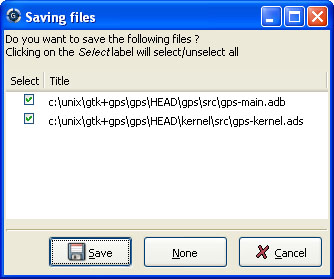
\includegraphics{save-dialog.jpg}

You can conveniently select or unselect all the files at once by clicking on
the title of the first column (labeled \emph{Select}). This will toggle the
selection status of the first line, and have the same status for all other
editors.

If you press \emph{Cancel} instead of \emph{Save}, no saving will take place, and the
action that displayed this dialog is also canceled. Such actions can be for
instance starting a compilation command, a VCS operation, or quitting GPS with
unsaved files.


\section{Remote Files}
\label{editing:remote-files}\label{editing:id19}
\index{remote files}
\index{ftp}
\index{ssh}
\index{rsh}
\index{rsync}
\index{telnet}
\index{http}
GPS has a basic support for working with files on remote hosts. This includes a
number of protocols, described below, which allow you to read a file from a
remote host, edit it locally, and then save it transparently to the remote
machine.

For now, the support for remote files is only available through the GPS shell
window. You start editing a remote file by typing a line similar to:

\begin{Verbatim}[commandchars=\\\{\}]
Editor.edit protocol://user@machine/full/path
\end{Verbatim}

where ``protocol'' should be replaced by the name of the protocol you want to
use, ``user'' is the login name you wish to use on the remote ``machine'', and
``/full/path'' is the full path on the remote machine to access the file.

The user name is optional. If it is the same as on the local machine, you can
omit the user name as well as the ``@'' sign.

Likewise, the machine name is optional, if you want to get a file from the
local host. This can be used to access files belonging to another user. In this
case, you need to specify the ``@'' sign, but do not insert a machine name right
after it.

Remote files can also be used if you want to work with GPS, but the machine on
which the files are found isn't supported by GPS.

The following protocols are supported:
\begin{description}
\item[{\emph{ssh}}] \leavevmode
This protocol is based on the ssh command line tool, which must therefore be
available in the path. It provides encrypted and secure connections to the
remote host. Files are transfered in-line, that is the connection is
established the first time you access the remote host, and kept open for all
further access.

\index{password}
Although ssh can be setup not to require a password, GPS will automatically
detect if a password is asked and open a dialog to query it.

The remote system must be a Unix-like system with support for standard Unix
commands like \emph{test}, \emph{echo}, \emph{rm} and \emph{ls}.

In the sample shell command above, you would replace the word ``protocol'' with
``ssh'' to use this protocol.

\item[{\emph{rsh}}] \leavevmode
This protocol behaves like ssh, except that the connections are not encrypted.
However, this protocol is generally available on all Unix machines by default.

It has the same requirements that the ssh protocol. To use it, substitute the
word ``rsh'' to ``protocol'' in the example above.

\item[{\emph{telnet}}] \leavevmode
This protocol is based on the standard telnet protocol. It behaves much like
the two protocols above, with an unencrypted connection.

To use it, substitute the word ``telnet'' to ``protocol'' in the example above.

\item[{\emph{scp}}] \leavevmode
This protocol is also based on one of the tools of the ssh suite. It provides
encrypted connections, and uses a mixture of ssh and scp connections.
Various commands like querying the time stamp of a file are executed through
a permanent ssh connection, whereas files are downloaded and uploaded through
a one-time scp command.

It basically has the same behavior as the ssh protocol, although it might be
slightly slower since a new connection has to be established every time a
file is fetched from, or written to the remote host. However, it might work
better than ssh if the file contains 8 bit characters.

To use it, substitute the word ``scp'' to ``protocol'' in the example above.

\item[{\emph{rsync}}] \leavevmode
Just like scp is based on ssh, this protocol is based on either rsh or ssh.
It depends on the external tool rsync, and uses a mixture of a rsh/ssh
connection for commands like querying the time stamp of a file, and one-time
connections with rsync to transfer the files.

Rsync is specially optimized to transfer only the parts of a file that are
different from the one already on the remote host. Therefore, it will
generally provide the best performance when writing the file back to the
remote host.

If you set up the environment variable RSYNC\_RSH to ssh before starting gps,
the connection will then be encrypted when transferring the files, and the
connection will be performed using ssh instead of rsh.

To use this protocol, substitute the word ``rsync'' to ``protocol'' in the
example above.

\item[{\emph{ftp}}] \leavevmode
This protocol provides only limited capabilities, but can be used to retrieve
or write a file back through an ftp connection, possibly even through an
anonymous ftp connection.

To use this protocol, substitute the word ``ftp'' to ``protocol'' in the example
above.

\item[{\emph{http}}] \leavevmode
This is the usual http protocol to download documents from the web. It is in
particular useful for documentation

\end{description}


\chapter{Source Navigation}
\label{navigation:id1}\label{navigation::doc}\label{navigation:source-navigation}
\index{source navigation}
\index{navigation}

\section{Support for Cross-References}
\label{navigation:support-for-cross-references}\label{navigation:id2}\label{navigation:index-1}
\index{cross-references}
GPS provides cross-reference navigation for program entities, such as types,
procedures, functions, variables, ..., defined in your application. The
cross-reference support in GPS relies on the compiler generated xref
information, which means that you need to either compile your project first
before being able to navigate, or use the menu \emph{Build-\textgreater{}Recompute Xref info}.
Similarly when your sources have been modified, you need to rebuild and
recompute xref information so that your changes are taken into account.

Here are language specific information about source navigation:
\begin{description}
\item[{\emph{Ada}}] \leavevmode
\index{Ada}
\index{GNAT}
The GNAT compiler is used to generate the cross-references information needed
by GPS by default, unless you are using the \emph{-gnatD} or \emph{-gnatx} switches, in
which case no cross reference information will be available.

\index{-gnatQ}
\index{-k}
If you need to navigate through sources that do not compile (e.g after
modifications, or while porting an application), GNAT can still generate
partial cross-reference information if you specify the \emph{-gnatQ} compilation
option. Along with the \emph{-k} option of gnatmake, it is then possible to
generate as much relevant information as possible for your non compilable
sources.

\index{ALI}
There are a few special cases where GPS cannot find the external file (called
\code{ALI file}) that contains the cross-reference information. Most likely,
this is either because you haven't compiled your sources yet, or because the
source code has changed since the \code{ALI file} was generated.

\index{project}
It could also be that you haven't included in the project the object
directories that contain the \code{ALI files}.

\index{separate unit}
In addition, one special case cannot be handled automatically. This is for
separate units, whose file names have been crunched through the \emph{gnatkr}
command. To handle this, you should force GPS to parse all the \code{ALI
files} in the appropriate object directory. This is done by right-clicking on
the object directory in the project view (left-side panel on the main
window), and selecting the menu ``Parse all xref information''.

\item[{\emph{C/C++}}] \leavevmode
\index{C}
\index{C++}
The GCC C and C++ compilers that come with GNAT need to be used to generate
the cross-references information needed by GPS, via the \emph{-fdump-xref} switch.
This means that you need to first add the \emph{-fdump-xref} switch to your
project's switches for C and C++ sources, and compile your application before
you browse through the cross-references or view various graphs in GPS.  If
sources have been modified, you should recompile the modified files.

\end{description}


\subsection{Loading xref info in memory}
\label{navigation:loading-xref-info-in-memory}
\index{Load xref info in memory}
The cross-reference information, as mentioned above, is generated either by the
compiler when you recompile your sources, or explicitly when you select the
menu \emph{Build-\textgreater{}Recompute Xref info}.

This information will be loaded in memory automatically by GPS when it needs
it, and as little as possible, to limit the memory footprint. However, this
means that some operations, for instance searching for all the references to a
global entity, will need to parse most, if not all, of the cross-reference
information. This will slow done the search the first time (and then the
information is in memory and the search is fast, unless the cross-reference
information has been regenerated on the disk).

You can select the menu \emph{Build-\textgreater{}Load xref info in memory} to force GPS to load
all the available information immediately in memory. This will speed up future
queries.

Note that GPS always loads all xref information for C and C++ sources in order
to provide accurate source navigation, so this menu is mainly relevant for Ada
sources.

A preference can be set to have GPS load the cross-information automatically on
startup, {\hyperref[extending:the-preferences-dialog]{\emph{The Preferences Dialog}}}.


\subsection{Ada xrefs heuristics}
\label{navigation:ada-xrefs-heuristics}
\index{Ada xrefs heuristics}
GPS is able to provide some basic navigation support for Ada sources in the
absence of information coming from the compiler. It uses a built-in Ada parser
parsing the Ada files at startup and allowing navigation in simple cases.

In this mode, GPS is able to navigate to an entity body from the declaration,
and to an entity declaration from the body. In case of other references, GPS
will navigate to the declaration on simple cases, namely if the heuristics
provide an information without ambiguity. In particular, it may not work with
overloaded entities.

These heuristics are not used in global reference searching operations or call
graphs.

Note that this parser is also used to provide the Ada outline view, code
completion and entity view.


\section{The Navigate Menu}
\label{navigation:the-navigate-menu}\label{navigation:id3}
\index{navigate}\begin{description}
\item[{\emph{Find or Replace...}}] \leavevmode
\index{find}
\index{search}
\index{replace}
Open the find and replace dialog. {\hyperref[searching:searching-and-replacing]{\emph{Searching and Replacing}}}.

\item[{\emph{Find Next}}] \leavevmode
\index{find next}
Find next occurrence of the current search. {\hyperref[searching:searching-and-replacing]{\emph{Searching and Replacing}}}.

\item[{\emph{Find Previous}}] \leavevmode
\index{find previous}
Find previous occurrence of the current search.
{\hyperref[searching:searching-and-replacing]{\emph{Searching and Replacing}}}.

\item[{\emph{Find All References}}] \leavevmode\phantomsection\label{navigation:find-all-references}
\index{find all references}
Find all the references to the current entity in the project. The search is
based on the semantic information extracted from the sources, this is not a
simple text search. The result of the search is displayed in the location
window, see {\hyperref[main_window:the-locations-view]{\emph{The Locations View}}}.

\item[{\emph{Goto Declaration}}] \leavevmode
\index{goto declaration}
Go to the declaration/spec of the current entity. The current entity is
determined by the word located around the cursor.  This item is also
accessible through the editor's contextual menu directly.  This capability
requires the availability of cross-reference information.
{\hyperref[navigation:support-for-cross-references]{\emph{Support for Cross-References}}}.

\item[{\emph{Goto Body}}] \leavevmode
\index{goto body}
Go to the body/implementation of the current entity. If the current entity is
the declaration of an Ada subprogram imported from C it goes to the location
where the C function is defined.  This item is also accessible through the
editor's contextual menu directly.  This capability requires the availability
of cross-reference information.  {\hyperref[navigation:support-for-cross-references]{\emph{Support for Cross-References}}}.

\item[{\emph{Goto Matching Delimiter}}] \leavevmode
\index{goto matching delimiter}
Go to the delimiter matching the one right before (for a closing delimiter) or
right after (for an opening delimiter) the cursor if any.

\item[{\emph{Goto Line...}}] \leavevmode
\index{goto line}
Open a dialog where you can type a line number,  in order to jump to a
specific location in the current source editor.

\item[{\emph{Goto Entity...}}] \leavevmode
\index{goto entity}
Open a dialog allowing browsing of the entities loaded in the project.  This
dialog functions similarly to {\hyperref[main_window:the-entity-view]{\emph{The Entity View}}}.

\item[{\emph{Goto File Spec\textless{}-\textgreater{}Body}}] \leavevmode
\index{goto file spec/body}
\index{Ada}
Open the corresponding spec file if the current edited file is a body file,
or body file otherwise. This option is only available for the Ada language.
This item is also accessible through the editor's contextual menu

This capability requires support for cross-references.  This item is also
accessible through the editor's contextual menu

\item[{\emph{Start Of Statement}}] \leavevmode
\index{Start Of Statement}
Move the cursor position to the start of the current statement, move to the
start of the enclosing statement if the cursor position is already at the
start of the statement.

\item[{\emph{End Of Statement}}] \leavevmode
\index{End Of Statement}
Move the current cursor position to the end of the statement, move to the end
of the enclosing statement if the cursor position is already at the end of
the statement.

\item[{\emph{Previous Subprogram}}] \leavevmode
\index{Previous Subprogram}
Move the current cursor position to the start of the previous procedure,
function, task, protected record or entry.

\item[{\emph{Next Subprogram}}] \leavevmode
\index{Next Subprogram}
Move the current cursor position to the start of the next procedure,
function, task, protected record or entry.

\item[{\emph{Previous Tag}}] \leavevmode
\index{tag}
\index{previous tag}
\index{locations view}
Go to previous tag/location. {\hyperref[main_window:the-locations-view]{\emph{The Locations View}}}.

\item[{\emph{Next Tag}}] \leavevmode
\index{tag}
\index{next tag}
\index{locations view}
Go to next tag/location. {\hyperref[main_window:the-locations-view]{\emph{The Locations View}}}.

\item[{\emph{Back}}] \leavevmode
\index{Back}
Go to previous location.

\item[{\emph{Forward}}] \leavevmode
\index{Forward}
Go to next location.

\end{description}


\section{Contextual Menus for Source Navigation}
\label{navigation:id4}\label{navigation:contextual-menus-for-source-navigation}
\index{contextual menu}
This contextual menu is available from any source editor.  If you right click
over an entity, or first select text, the contextual menu will apply to this
selection or entity.
\begin{description}
\item[{\emph{Goto declaration of *entity*}}] \leavevmode
\index{goto declaration}
Go to the declaration/spec of \emph{entity}. The current entity is determined by
the word located around the cursor or by the current selection if any.  This
capability requires support for cross-references.

\item[{\emph{Goto full declaration of *entity*}}] \leavevmode
\index{goto declaration}
This contextual menu appears for a private or limited private types. Go to
the full declaration/spec of \emph{entity}. The current entity is determined by
the word located around the cursor or by the current selection if any.  This
capability requires support for cross-references.

\item[{\emph{Goto type declaration of *entity*}}] \leavevmode
\index{goto type declaration}
Go to the type declaration of \emph{entity}. The current entity is determined by
the word located around the cursor or by the current selection if any.  This
capability requires support for cross-references.

\item[{\emph{Display type hierarchy for *entity*}}] \leavevmode
\index{display type hierarchy}
This contextual menu appears for derived or access types. Output the type
hierarchy for \emph{entity} into the location view. The current entity is
determined by the word located around the cursor or by the current selection
if any.  This capability requires support for cross-references.

\item[{\emph{Goto body of *entity*}}] \leavevmode
\index{goto body}
Go to the body/implementation of \emph{entity}. If \emph{entity} is the declaration of
an Ada subprogram imported from C it goes to the the location where the C
function is defined.  This capability requires support for cross-references.

\item[{\emph{Goto declarations of *entity*}}] \leavevmode
\index{goto declaration}
This contextual menu appears when you are clicking on a subprogram call that
is a dispatching call. In such a case, there is no possibility for GPS to
know what subprogram will actually be called at run time, since that depends
on dynamic information. It therefore gives you a list of all entities in the
tagged type hierarchy, and lets you choose which of the declarations you want
to jump to. See also the \code{methods.py} plug-in (enabled by default)
which, given an object, lists all its primitive operations in a contextual
menu so that you can easily jump to them. See also the contextual menu
\code{References/Find References To...} which allows you to find all calls
to a subprogram or to one of its overriding subprograms.

\item[{\emph{Goto bodies of *entity*}}] \leavevmode
\index{goto body}
This is similar to \emph{Goto declarations of}, but applies to the bodies of the
entities.

\item[{\emph{Goto file spec/body}}] \leavevmode
\index{goto file spec/body}
\index{Ada}
Open the corresponding spec file if the current edited file is a body file,
or body file otherwise. This option is only available for the Ada language.

\item[{\emph{Entity} calls}] \leavevmode
Display a list of all subprograms called by \emph{entity} in a tree view. This is
generally more convenient than using the corresponding Browsers/ submenu if
you expect lots of references, {\hyperref[main_window:the-callgraph-view]{\emph{The Callgraph View}}}.

\item[{\emph{Entity} is called by}] \leavevmode
Display a list of all subprograms calling \emph{entity} in a tree view. This is
generally more convenient than using the correponding Browsers/ submenu if
you expect lots of references, {\hyperref[main_window:the-callgraph-view]{\emph{The Callgraph View}}}.

\item[{References}] \leavevmode
\index{references}
This item gives access to different capabilities related to listing or
displaying references to the current entity or selection.

\item[{\emph{Find all references to *entity*}}] \leavevmode
\index{find all references}
{\hyperref[navigation:find-all-references]{\emph{Find all references}}} to \emph{entity} in all the
files in the project.

\item[{\emph{Find all references...}}] \leavevmode
This menu is similar to the one above, except it is possible to select more
precisely what kind of reference should be selected. It is also possible to
indicate the scope of the search, and whether the context (or caller) at
each reference should be displayed. Computing the caller information will
take slightly longer though.

\index{primitive operation}
This dialog has an option \emph{Include overriding and overriden operations},
which, when activated, will include references to overriden or overriding
entities of the one you selected.

This is particularly useful when you are wondering whether you can easily
modify the profile of a primitive operation, since you can then see what
other entities will also be impacted. If you select only the \emph{declaration}
check box, you will see the list of all related primitive operations.

\index{imported entities}
This dialog also allows you to find out which entities are imported from a
given file/unit. Click on any entity from that file (for instance on the
\emph{with} line for Ada code), then select the \emph{All entities imported from same
file} toggle button. This will display in the location window the list of
all entities imported from the same file as the entity selected.

In addition, if you have selected the \emph{Show context} option, you will get a
list of all the exact references to these entities within the file.
Otherwise, you just get a pointer to the declaration of the imported
entities.

\item[{\emph{Find all local references to *entity*}}] \leavevmode
\index{find all local references}
{\hyperref[navigation:find-all-references]{\emph{Find all references}}} to \emph{entity} in the current
file (or in the current top level unit for Ada sources).  details.

\item[{\emph{Variables used in *entity*}}] \leavevmode
\index{variables used}
Find all variables (local or global) used in \emph{entity} and list each first
reference in the locations window.

\item[{\emph{Non Local variables used in *entity*}}] \leavevmode
Find all non-local variables used in the entity.

\item[{\emph{Methods of *entity*}}] \leavevmode
\index{methods}
\index{primitive operations}
This submenu is only visible if you have activated the plug-in
\code{methods.py} (which is the case by default), and when you click on a
tagged type or an instance of a tagged type. This menu lists all the
primitive operations of that type, and you can therefore easily jump to the
declaration of any of these operations.

\item[{\emph{Browsers}}] \leavevmode
\index{browsers}
This item gives access to graph representations of callers and callees for
subprograms.
\begin{description}
\item[{\emph{Entity} calls}] \leavevmode
\index{call graph}
\index{calls}
Open or raise the call graph browser on the specified entity and display
all the subprograms called by \emph{entity}. {\hyperref[browsing:call-graph]{\emph{Call Graph}}}.

\item[{\emph{Entity} calls (recursively)}] \leavevmode
\index{call graph}
\index{calls}
Open or raise the call graph browser on the specified entity and display
all the subprograms called by \emph{entity}, transitively for all subprograms.
Since this can take a long time to compute and generate a very large graph,
an intermediate dialog is displayed to limit the number of subprograms to
display (1000 by default). {\hyperref[browsing:call-graph]{\emph{Call Graph}}}.

\item[{\emph{Entity} is called by}] \leavevmode
\index{call graph}
\index{called by}
Open or raise the call graph browser on the specified entity and display
all the subprograms calling \emph{entity}. {\hyperref[browsing:call-graph]{\emph{Call Graph}}}.

Note that this capability requires a global look up in the project
cross-references, which may take a significant amount of time the first
time.  After a global look up, information is cached in memory, so that
further global queries will be faster.

\end{description}

\item[{Expanded code}] \leavevmode
Present for Ada files only. This menu generates a .dg file using your gnat
compiler (using the -gnatGL switch) and displays the expanded code. This can
be useful when investigating low-level issues and tracing precisely how the
source code is transformed by the GNAT front-end.
\begin{description}
\item[{\emph{Show subprogram}}] \leavevmode
Display expanded code for the current subprogram in the current editor.

\item[{\emph{Show file}}] \leavevmode
Display expanded code for the current file in the current editor.

\item[{\emph{Show in separate editor}}] \leavevmode
Display expanded code for the current file in a new editor.

\item[{\emph{Clear}}] \leavevmode
Remove expanded code from the current editor.

\end{description}

For Ada files only, this entry will generate, and will open this file
at the location corresponding to the current source line.

\item[{\emph{Open \textless{}filename\textgreater{}}}] \leavevmode
When you click on a filename (for instance a C' \emph{\#include}, or an error
message in a log file), this menu gives you a way to open the corresponding
file. If the file name was followed by '':'' and a line number, the
corresponding line is activated.

\end{description}


\section{Navigating with hyperlinks}
\label{navigation:id5}\label{navigation:navigating-with-hyperlinks}
\index{hyperlinks}
When the Control key is pressed and you start moving the mouse, entities in the
editors under the mouse cursor become hyperlinks and the mouse cursor aspect
changes.

Left-clicking on a reference to an entity will open a source editor on the
declaration of this entity, and left-clicking on an entity declaration will
open an editor on the implementation of this entity.

Left-clicking on the Ada declaration of a subprogram imported from C will open
a source editor on the definition of the corresponding C entity. This
capability requires support for cross-references.

Clicking with the middle button on either a reference to an entity or the
declaration of an entity will jump directly to the implementation or type
completion) of this entity.

Note that for efficiency, GPS may create hyperlinks for some entities which
have no associated cross reference. In this case, clicking will have no effect,
even though an hyperlink may have been displayed.

This behavior is controlled by the \emph{Hyper links} preference.


\section{Highlighting dispatching calls}
\label{navigation:id6}\label{navigation:highlighting-dispatching-calls}
\index{dispatching}
Dispatching calls in Ada and C++ source code are highlighted by default in GPS
via the \emph{dispatching.py} plug-in.

Based on the cross-reference information, this plug-in will highlight (with a
special color that you can configure in the preferences dialog) all calls that
are dispatching (or calls to virtual methods in C++).  A dispatching call, in
Ada, is a subprogram call where the actual subprogram that is called is not
known until run time, and is chosen based on the tag of the object (so this of
course only exists when you are using object-oriented programming).

To disable this highlighting (which might sometimes be slow if you are using
big sources, even though the highlighting itself is done in the background),
you can go to the \emph{/Tools/Plug-ins} menu, and disable the \emph{dispatching.py}
plug-in.


\chapter{Project Handling}
\label{projects:project-handling}\label{projects::doc}\label{projects:id1}
\index{project}
\index{project view}
The section on the project view ({\hyperref[projects:the-project-view]{\emph{The Project View}}}) has already given a
brief overview of what the projects are, and the information they contain.

This chapter provides more in-depth information, and describes how such
projects can be created and maintained.


\section{Description of the Projects}
\label{projects:id2}\label{projects:description-of-the-projects}
\index{project description}

\subsection{Project files and GNAT tools}
\label{projects:project-files-and-gnat-tools}\label{projects:index-2}
\index{project file}
\index{GNAT}
This section describes what the projects are, and what information they
contain.

The most important thing to note is that the projects used by GPS are the same
as the ones used by GNAT. These are text files (using the extension
\code{.gpr}) which can be edited either manually, with any text editor, or
through the more advanced GPS interface.

The exact syntax of the project files is fully described in the GNAT User's
Guide (gnat\_ug.html) and GNAT Reference Manual (gnat\_rm.html). This is recommended reading if you want to use some of the
more advanced capabilities of project files which are not yet supported by the
graphical interface.

GPS can load any project file, even those that you have been edited manually.
Furthermore, you can manually edit project files created by GPS.

Typically you will not need to edit project files manually, since several
graphical tools such as the project wizard ({\hyperref[projects:the-project-wizard]{\emph{The Project Wizard}}}) and the
properties editor({\hyperref[projects:the-project-properties-editor]{\emph{The Project Properties Editor}}}) are provided.

\index{normalization of projects}
GPS doesn't preserve the layout nor comments of manually created projects after
you have edited them in GPS. For instance, multiple case statements in the
project will be coalesced into a single case statement.  This normalization is
required for GPS to be able to preserve the previous semantic of the project in
addition to the new settings.

\index{GNAT}
All command-line GNAT tools are project aware, meaning that the notion of
project goes well beyond GPS' user interface. Most capabilities of project
files can be accessed without using GPS itself, making project files very
attractive.

\index{ADA\_PROJECT\_PATH}
GPS uses the same mechanisms to locate project files as GNAT itself:
\begin{itemize}
\item {} 
absolute paths

\item {} 
relative paths.
These paths, when used in a with line as described below, are relative
to the location of the project that does the with.

\item {} 
ADA\_PROJECT\_PATH.
If this environment variable is set, it contains a colon-separated (or
semicolon under Windows) list of directories in which the project files are
searched.

\item {} 
predefined project path.
The compiler itself defines a predefined project path, in which standard
libraries can be installed, like XML/Ada for instance.

\end{itemize}


\subsection{Contents of project files}
\label{projects:contents-of-project-files}
\index{project file}
Project files contain all the information that describe the organization of
your source files, object files and executables.

\index{project comments}
A project file can contain comments, which have the same format as in Ada, that
is they start by ``--'' and extend to the end of the line.  You can add comments
when you edit the project file manually. GPS will attempt to preserve them when
you save the project through the menu, but this will not always be possible. It
helps if the comments are put at the end of the line, as in:

\begin{Verbatim}[commandchars=\\\{\}]
\PYG{n}{project} \PYG{n}{Default} \PYG{k+kr}{is}
    \PYG{k+kr}{for} \PYG{n}{Source\PYGZus{}Dirs} \PYG{k+kn}{use} \PYG{p}{(}\PYG{p}{)}\PYG{p}{;}  \PYG{c+c1}{--  No source in this project}
\PYG{k+kr}{end} \PYG{n+nf}{Default}\PYG{p}{;}
\end{Verbatim}

\index{sub project}
Generally, one project file will not be enough to describe a complex
organization. In this case, you will create and use a project hierarchy, with a
root project importing other sub projects. Each of the projects and sub
projects is responsible for its own set of sources (compiling them with the
appropriate switches, put the resulting files in the right directories, ...).

\index{GNAT}
Each project contains the following information (see the GNAT user's guide for
the full list)
\begin{itemize}
\item {} 
\textbf{List of imported projects}:
.. index:: imported project

When you are compiling sources from this project, the builder will first make
sure that all the imported projects have been correctly recompiled and are
up-to-date. This way, dependencies between source files are properly handled.

If one of the source files of project A depends on some source files from
project B, then B must be imported by A. If this isn't the case, the compiler
will complain that some of the source files cannot be found.

One important rule is that each source file name must be unique in the
project hierarchy (i.e. a file cannot be under control of two different
projects). This ensures that the same file will be found no matter what
project is managing the source file that uses

\item {} 
\textbf{List of source directories}:
.. index:: source directory

All the sources managed by a project are found in one or more source
directories. Each project can have multiple source directories, and a given
source directory might be shared by multiple projects.

\item {} 
\textbf{Object directory}:
.. index:: object directory

When the sources of the project are compiled, the resulting object files are
put into this object directory. There exist exactly one object directory for
each project. If you need to split the object files among multiple object
directories, you need to create multiple projects importing one another as
appropriate.

When sources from imported sub-projects are recompiled, the resulting object
files are put in the sub project's own object directory, and will never
pollute the parent's object directory.

\item {} 
\textbf{Exec directory}:
.. index:: exec directory

When a set of object files is linked into an executable, this executable is
put in the exec directory of the project file. If this attribute is
unspecified, the object directory is used.

\item {} 
\textbf{List of source files}:
.. index:: source file

The project is responsible for managing a set of source files. These files
can be written in any programming languages. Currently, the graphical
interface supports Ada, C and C++.

The default to find this set of source files is to take all the files in the
source directories that follow the naming scheme (see below) for each
language. In addition if you edit the project file manually, it is possible
to provide an explicit list of source files.

This attribute cannot be modified graphically yet.

\item {} 
\textbf{List of main units}:
.. index:: main unit

The main units of a project (or main files in some languages) are the units
that contain the main subprogram of the application, and that can be used to
link the rest of the application.

The name of the file is generally related to the name of the executable.

A given project file hierarchy can be used to compile and link several
executables. GPS will automatically update the Compile, Run and Debug menu
with the list of executables, based on this list.

\item {} 
\textbf{Naming schemes}:
.. index:: naming scheme

The naming scheme refers to the way files are named for each languages of the
project. This is used by GPS to choose the language support to use when a
source file is opened. This is also used to know what tools should be used to
compile or otherwise work with a source file.

\item {} 
\textbf{Embedded targets and cross environments}:
.. index:: cross environment

GPS supports cross environment software development: GPS itself can run on a
given host, such as GNU/Linux, while compilations, runs and debugging occur
on a different remote host, such as Sun/Solaris.

\index{VxWorks}
GPS also supports embedded targets (VxWorks, ...) by specifying alternate
names for the build and debug tools.

The project file contains the information required to log on the remote host.

\item {} 
\textbf{Tools}:
.. index:: tools

Project files provide a simple way to specify the compiler and debugger
commands to use.

\item {} 
\textbf{Switches}:
.. index:: switches

Each tool that is used by GPS (compiler, pretty-printer, debugger, ...) has
its own set of switches. Moreover, these switches may depend on the specific
file being processed, and the programming language it is written in.

\end{itemize}


\section{Supported Languages}
\label{projects:id3}\label{projects:supported-languages}
\index{languages}
\index{text files}
Another information stored in the project is the list of languages that this
project knows about. GPS support any number of language, with any name you
choose. However, advanced support is only provided by default for some
languages (Ada, C and C++), and you can specify other properties of the
languages through customization files
({\hyperref[extending:adding-support-for-new-languages]{\emph{Adding support for new languages}}}).

By default, the graphical interface will only give you a choice of languages
among the ones that are known to GPS at that point, either through the default
GPS support or your customization files. But you can also edit the project
files by hand to add support for any language.

Languages are a very important part of the project definition. For each
language, you should specify a naming scheme that allows GPS to associate files
with that language. You would for instance specify that all \code{.adb} files
are Ada, all \code{.txt} files are standard text files, and so on.

Only the files that have a known language associated with them are displayed in
the \emph{Project View}, or available for easy selection through the \emph{File-\textgreater{}Open
From Project} menu. Similarly, only these files are shown in the Version
Control System interface.

It is therefore important to properly setup your project to make these files
available conveniently in GPS, although of course you can still open any file
through the \emph{File-\textgreater{}Open} menu.

If your project includes some README files, or other text files, you should add
``txt'' as a language (or any other name you want), and make sure that these
files are associated with that language in the \emph{Project properties editor}.

By default, GPS provides support for a number of languages. In most cases, this
support takes the form of syntax highlighting in the editor, and possibly the
Outline View. Other languages have advanced cross-references available.

All the supported languages can be added to the project, but you can also add
your own languages as you need (either by editing the project files by hand, or
by creating XML files to add GPS support for these languages, which will then
show in the project properties editor graphically).


\section{Scenarios and Configuration Variables}
\label{projects:id4}\label{projects:scenarios-and-configuration-variables}
\index{configuration variable}
\index{project variable}
\index{variable}
The behavior of projects can be further tailored by the use of scenarios.

\index{project attribute}
All the attributes of a project, except its list of imported projects, can be
chosen based on the value of external variables, whose value is generally
coming from the host computer environment, or directly set in GPS. The
interface to manipulate these scenarios is the scenario view, which can be
displayed by selecting the menu \emph{Tools-\textgreater{}Views-\textgreater{}Scenario}.  It can be convenient
to drag this window with your mouse, and drop it above the project view, so
that you can see both at the same time.

This area allows you to select new values for the scenario variables defined in
your project, and thus change dynamically the view GPS has of your project and
your source files.

\index{compile}
\index{debug}
This facility can for instance be used to compile all the sources either in
debug mode (so that the executables can be run in the debugger), or in
optimized mode (to reduce the space and increase the speed when delivering the
software).  In this configuration scenario, all the attributes (source
directories, tools, ...) remain the same, except for the compilation switches.
It would be more difficult to maintain a completely separate hierarchy of
project, and it is much more efficient to create a new configuration variable
and edit the switches for the appropriate scenario
({\hyperref[projects:the-project-properties-editor]{\emph{The Project Properties Editor}}}).

There is one limitation in what GPS can do with scenario variables: although
gnatmake and gprbuild have no problem dealing with scenario variables whose
default value is not a static string (for instance a concatenation, or the
value of another scenario variable), GPS will not be able to edit such a
project graphically. Such projects will load fine in GPS though.


\subsection{Creating new configuration variables}
\label{projects:creating-new-configuration-variables}
\index{creating configuration variable}
Creating a new scenario variable is done through the contextual menu
(right-click) in the Project View or the Scenario View itself. Select the menu
\emph{Project-\textgreater{}Add Configuration Variable}. This opens the following dialog:

\index{screen shot}
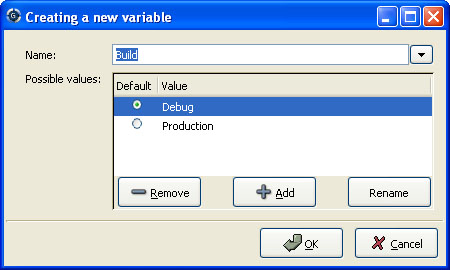
\includegraphics{scenarios.jpg}

There are two main areas in this dialog: in the top line, you specify the name
of the variable. This name is used for two purposes:
\begin{itemize}
\item {} 
It is displayed in the scenario view
.. index:: scenario view

\item {} 
This is the name of the environment variable from which the initial value is
read. When GPS is started, all configuration variables are initialized from
the host computer environment, although you can of course change its value
later on inside GPS. Note that selecting a new value for the scenario
variable does not change the actual value of the environment variable, which
is only used to get the default initial value of the scenario variable.

When you spawn external tools like gnatmake for instance, you can also
specify the value they will use for the scenario variable by using a command
line switch, typically \emph{-X}.

\end{itemize}

If you click on the arrow on the right of this name area, GPS will display the
list of all the environment variables that are currently defined. However, you
don't need to pick the name of an existing variable, neither must the variable
exist when GPS is started.

The second part of this dialog is the list of authorized value for this
variable. Any other value will generate an error reported by GPS, and the
project won't be loaded as a result.

One of these values is the default value (the one whose button in the Default
column is selected). This means that if the environment variable doesn't exist
when GPS is started, GPS will behave as if it did exist with this default
value.

The list of possible values can be edited by right-clicking on the name of the
variable, and selecting one of \emph{Edit properties} or \emph{Delete variable}.


\subsection{Editing existing configuration variables}
\label{projects:editing-existing-configuration-variables}
\index{editing configuration variable}
If at least one configuration variable is defined in your project, the scenario
view will contain something similar to:

\index{screen shot}
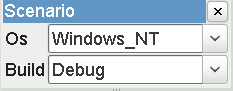
\includegraphics{explorer-scenario.jpg}

\index{Unix}
This screen shot shows two configuration variables, named \emph{Build} and \emph{OS},
with their current value (resp. \emph{Debug} and \emph{Unix}).

You can easily change the current value of any of these variables by clicking
on the arrow on the right of the value. This will display a pop-up window with
the list of possible values, from which you select the one you wish to use.

As soon as a new value is selected, GPS will recompute the project view (in
case source directories, object directories or list of source files have
changed). A number of things will also be updated (like the list of executables
in the \emph{Compile}, \emph{Run} and \emph{Debug} menus).

\index{browsers}
\index{call graph}
Currently, GPS will not recompute the contents of the various browsers (call
graph, dependencies, ...) for this updated project. This would be too expensive
to do every time the value changes, and therefore you need to explicitly
request an update.

You can change the list of possible values for a configuration variable at any
time by clicking on the button to the far left of the variable's name. This
will pop up the same dialog that is used to create new variables. This dialog
also allows you to change the name of the scenario variable. This name is the
same as the environment variable that is used to set the initial value of the
scenario variable.

\index{removing variable}
Removing a variable is done by clicking on the button immediately to the left
of the variable's name. GPS will then display a confirmation dialog.

If you confirm that you want to delete the variable, GPS will simply remove the
variable, and from now on act as if the variable always had the value it had
when it was deleted.


\section{Extending Projects}
\label{projects:id5}\label{projects:extending-projects}
\index{projects}\index{extending}

\subsection{Description of extending projects}
\label{projects:index-29}\label{projects:description-of-extending-projects}
The project files were designed to support big projects, with several hundreds
or thousands of source files. In such contexts, one developer will generally
work on a subset of the sources. It is also not rare for such a project to take
several hours to fully compile. Most developers therefore do not need to have
the full copy of the project compiled on their own machine or personal disk
space.

However, it is still useful to be able to access other source files of the
application, for instance to find out whether a subprogram can be changed and
where it is currently called.

Such a setup can be achieved through extending projects. These are special
types of projects that inherit most of their attributes and source files from
another project, and can have, in their source directories, some source files
that hide/replace those inherited from the original project.

When compiling such projects, the compiler will put the newly created project
files in the extending project's directory, and will leave the original
untouched. As a result, the original project can be shared read-only among
several developers (for instance, it is usual for this original project to be
the result of a nightly build of the application).


\subsection{Creating extending projects}
\label{projects:creating-extending-projects}
This project wizard allows you to easily create extending projects. You should
select an empty directory (which will be created automatically if needed), as
well as a list of source files you want to work on initially.  New files can
also be added later.

As a result, GPS will copy the selected source files to the new directory (if
you so decided), and create a number of project files there. It will then load
a new project, which has the same properties as the previous one, except that
some files are found transparently in the new directory, and object files
resulting from the compilation are create into that directory as opposed to the
object directory of the original project.


\subsection{Adding files to extending projects}
\label{projects:adding-files-to-extending-projects}
\index{Add To Extending Project}
Once you have loaded an extending project in GPS, things work mostly
transparently. If you open a file through the \emph{File-\textgreater{}Open From Project} dialog,
the files found in the local directory of your extending project will be picked
up first.

The build actions will create object files in the extending project's
directory, leaving the original project untouched.

It might happen that you want to start working on a source file that you had
not added in the extending project when it was created. You can of course edit
the file found in the original project, provided you have write access to it.
However, it is generally better to edit it in the context of the extending
project, so that the original project can be shared among developers.

This can be done by clicking on the file in the \emph{Project View}, then selecting
the menu \emph{Add To Extending Project}. This will popup a dialog asking whether
you want GPS to copy the file to the extending project's directory for you. GPS
might also create some new project files in that directory if necessary, and
automatically reload the project as needed. From then on, if you use the menu
\emph{File-\textgreater{}Open From Project}, GPS will first see the file from the extending
project.

Note that open editors will still be editing the same file they were before, so
you should open the new file if needed.


\section{The Project View}
\label{projects:id6}\label{projects:the-project-view}
\index{project view}
The project view, as mentioned in the general description of the GPS window, is
one of the views found by default on the left of the window. It shows in a tree
structure the project hierarchy, along with all the source files belonging to
the project, and the entities declared in the source files.

It is worth noting that the project view provides a tree representation of the
project hierarchy. If a project is imported by multiple other projects in the
hierarchy, then this project will appear multiple times in the project view.

\index{limited with}
Likewise, if you have edited the project manually and have used the \emph{limited
with} construct to have cycles in the project dependencies, the cycle will
expand infinitely. For instance, if project \code{a} imports project
\code{b}, which in turns imports project \code{a} through a \emph{limited with}
clause, then expanding the node for \code{a} will show \code{b}. In turn,
expanding the node for \code{b} will show a node for \code{a}, and so on.

The contextual menu in this project view provides a number of items to modify
the project hierarchy (what each project imports), as well as to visualize and
modify the attributes for each projects (compilation switches, naming scheme,
...)

The following entries are available in the contextual menu:
\begin{description}
\item[{\emph{Show Projects Imported by...}}] \leavevmode
This item will open a new window in GPS, the project browser, which
displays graphically the relationships between each project in the
hierarchy.

\item[{\emph{Save The Project...}}] \leavevmode
\index{saving projects}
This item can be selected to save a single project in the hierarchy after it
was modified. Modified but unsaved projects in the hierarchy have a special
icon (a pen mark is drawn on top of the standard icon). If you would rather
save all the modified projects in a single step, use the menu bar item
\emph{Project-\textgreater{}Save All}.

\item[{\emph{Project/Properties}}] \leavevmode
This item will open a new dialog, and give access to all the
attributes of the project: tool switches, naming schemes, source
directories, ... {\hyperref[projects:the-project-properties-editor]{\emph{The Project Properties Editor}}}.

\item[{\emph{Project/Edit source file}}] \leavevmode
\index{edit project source file}
This menu will load the project file into an editor, so that you can manually
edit it. This should be used if you need to access some features of the
project files that are not accessible graphically (renames statements,
variables, ...)

\item[{\emph{Project/Dependencies...}}] \leavevmode
\index{project dependency}
This opens the dependencies editor ({\hyperref[projects:the-project-dependencies-editor]{\emph{The Project Dependencies Editor}}}).

\item[{\emph{Add Configuration Variable}}] \leavevmode
\index{add configuration variable}
This menu item should be used to add new configuration variables, as
described in {\hyperref[projects:scenarios-and-configuration-variables]{\emph{Scenarios and Configuration Variables}}}.

\item[{\emph{Build}}] \leavevmode
This menu offers the submenu ``Clean'' which remove all object files and other
compilation artifacts associated to the current project.

\end{description}

\index{saving projects}
Any time one or several projects are modified, the contents of the project view
is automatically refreshed. No project is automatically saved. This provides a
simple way to temporarily test new values for the project attributes.  Unsaved
modified projects are shown with a special icon in the project view, displaying
a pen mark on top of the standard icon:

\index{screen shot}

\includegraphics{project-modified.jpg}

Note that in all tree views in GPS, you can use the \code{+} and \code{-} keys
to expand and collapse nodes (e.g. projects and directories).


\section{Disabling Project Edition Features}
\label{projects:id7}\label{projects:disabling-project-edition-features}
\index{project editing}
The project files should generally be considered as part of the sources, and
thus be put under control of a version control system. As such, you might want
to prevent accidental editing of the project files, either by you or some other
person using the same GPS installation.

The main thing to do to prevent such accidental edition is to change the write
permissions on the project files themselves. On Unix systems, you could also
change the owner of the file. When GPS cannot write a project file, it will
report an error to the user.

However, the above doesn't prevent a user from trying to do some modifications
at the GUI level, since the error message only occurs when trying to save the
project (this is by design, so that temporary modification can be done in
memory).

You can disable all the project editing related menus in GPS by adding special
startup switches. The recommended way is to create a small batch script that
spawns GPS with these switches. You should use the following command line:

\begin{Verbatim}[commandchars=\\\{\}]
\PYG{n}{gps} \PYG{c+c1}{--traceoff=MODULE.PROJECT\PYGZus{}VIEWER --traceoff=MODULE.PROJECT\PYGZus{}PROPERTIES}
\end{Verbatim}

What these do it prevent the loading of the two GPS modules that are
responsible for project edition. However, this also has an impact on the python
functions that are exported by GPS, and thus could break some plug-ins. Another
solution which might apply in your case is simply to hide the corresponding
project-editing menus and contextual menus. This could be done by creating a
small python plugin for GPS ({\hyperref[extending:customizing-through-xml-and-python-files]{\emph{Customizing through XML and Python files}}},
which contains the following code:

\begin{Verbatim}[commandchars=\\\{\}]
\PYG{k+kn}{import} \PYG{n+nn}{GPS}
\PYG{n}{GPS}\PYG{o}{.}\PYG{n}{Menu}\PYG{o}{.}\PYG{n}{get}  \PYG{p}{(}\PYG{l+s}{"}\PYG{l+s}{/Project/Edit Project Properties}\PYG{l+s}{"}\PYG{p}{)}\PYG{o}{.}\PYG{n}{hide}\PYG{p}{(}\PYG{p}{)}
\PYG{n}{GPS}\PYG{o}{.}\PYG{n}{Contextual} \PYG{p}{(}\PYG{l+s}{'}\PYG{l+s}{Edit project properties}\PYG{l+s}{'}\PYG{p}{)}\PYG{o}{.}\PYG{n}{hide}\PYG{p}{(}\PYG{p}{)}
\PYG{n}{GPS}\PYG{o}{.}\PYG{n}{Contextual} \PYG{p}{(}\PYG{l+s}{'}\PYG{l+s}{Save project}\PYG{l+s}{'}\PYG{p}{)}\PYG{o}{.}\PYG{n}{hide}\PYG{p}{(}\PYG{p}{)}
\PYG{n}{GPS}\PYG{o}{.}\PYG{n}{Contextual} \PYG{p}{(}\PYG{l+s}{'}\PYG{l+s}{Add configuration variable}\PYG{l+s}{'}\PYG{p}{)}\PYG{o}{.}\PYG{n}{hide}\PYG{p}{(}\PYG{p}{)}
\end{Verbatim}


\section{The Project Menu}
\label{projects:id8}\label{projects:the-project-menu}
\index{project menu}
The menu bar item \emph{Project} contains several commands that generally act on the
whole project hierarchy. If you only want to act on a single project, use the
contextual menu in the project view.

Some of these menus apply to the currently selected project. This notion
depends on what window is currently active in GPS: if it is the project view,
the selected project is either the selected node (if it is a project), or its
parent project (for a file, directory, ...).  If the currently active window is
an editor, the selected project is the one that contains the file.

In all cases, if there is no currently selected project, the menu will apply to
the root project of the hierarchy.

These commands are:
\begin{description}
\item[{\emph{New}}] \leavevmode
This menu will open the project wizard ({\hyperref[projects:the-project-wizard]{\emph{The Project Wizard}}}), so
that you can create new project. On exit, the wizard asks whether the
newly created project should be loaded. If you select \emph{Yes}, the new
project will replace the currently loaded project hierarchy.

You will get asked what information you would like to create the project
from.  In particular, you can create a set of project files from existing Ada
sources.

\item[{\emph{New from template}}] \leavevmode
This menu will open the project template wizard, allowing you to create a new
project using one of the project templates defined in GPS.
{\hyperref[extending:adding-project-templates]{\emph{Adding project templates}}}.

\item[{\emph{Open}}] \leavevmode
This menu opens a file selection dialog, so that any existing project
can be loaded into GPS. The newly loaded project replaces the currently
loaded project hierarchy. GPS works on a single project hierarchy at
a time.

\item[{\emph{Recent}}] \leavevmode
This menu can be used to easily switch between the last projects that
were loaded in GPS.

\item[{\emph{Edit Project Properties}}] \leavevmode
This menu applies to the currently selected project, and will open the
project properties dialog for this project.

\item[{\emph{Save All}}] \leavevmode
This will save all the modified projects in the hierarchy.

\item[{\emph{Edit File Switches}}] \leavevmode\phantomsection\label{projects:file-switches}
This menu applies to the currently selected project. This will open a new
window in GPS, listing all the source files for this project, along with the
switches that will be used to compile them, {\hyperref[projects:the-switches-editor]{\emph{The Switches Editor}}}.

\item[{\emph{Reload Project}}] \leavevmode
\index{reload project}
\index{C}
\index{C++}
Reload the project from the disk, to take into account modifications done
outside of GPS. In particular, it will take into account new files added
externally to the source directories.  This isn't needed for modifications
made through GPS.

\item[{\emph{Project View}}] \leavevmode
Open (or raise if it is already open) the project view on the left side
of the GPS window.

\end{description}


\section{The Project Wizard}
\label{projects:the-project-wizard}\label{projects:id9}
\index{project wizard}
The project wizard allows you to create in a few steps a new project file.  It
has a number of pages, each dedicated to editing a specific set of attributes
for the project.

The typical way to access this wizard is through the \emph{Project-\textgreater{}New...} menu.

The project wizard is also launched when a new dependency is created between
two projects, through the contextual menu in the project view.

\index{screen shot}
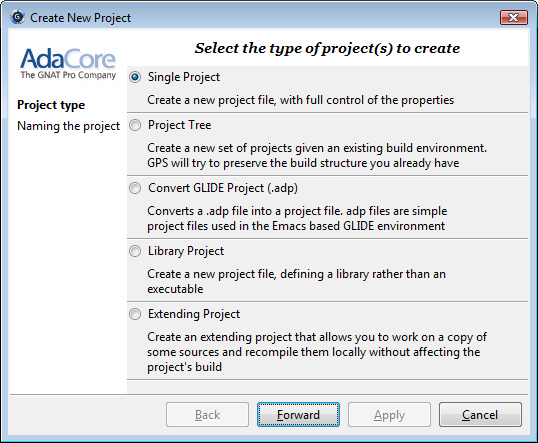
\includegraphics{project-wizard.jpg}

The wizard gives access to the following list of pages:
\begin{itemize}
\item {} 
Project type

\item {} 
Project Naming

\item {} 
Languages Selection

\item {} 
Version Control System Selection

\item {} 
Source Directories Selection

\item {} 
Build Directory

\item {} 
Main Units

\item {} 
Library

\item {} 
Naming Scheme

\item {} 
Switches

\end{itemize}


\subsection{Project Type}
\label{projects:project-type}
Several types of project wizards are provided in GPS. Depending on the
information you have or your current setup, you will choose one or the other.
\begin{itemize}
\item {} 
Single Project

This is likely the wizard you will use most often. It creates a project file
from scratch, and asks you for the location of source directories, the object
directory, ...; The rest of this chapter describes this wizard in more
details

\item {} 
Project Tree

This wizard will attempt to create a set of one or more project files to
represent your current build environment. It will analyze what your sources
are, where the corresponding object files are, and will try and find some
possible setup for the project files (remember that a given \code{.gpr}
project file can be associated with a single object directory.

This wizard might not work in all cases, but is worth a try to get you
started if you already have an existing set of sources

\item {} 
Convert GLIDE Project (.adp)

This wizard will help you convert a \code{.adp} project file that is used by
the GLIDE environment. The same restrictions apply as above, except that the
list of source directories, object directories and tool switches are read
directly from that file.

\item {} 
Library Project
.. index:: project, library

This specialized wizard is similar to the Single Project wizard, except it
adds one extra page, the Library page. The output of the compilation of this
project is a library (shared or static), as opposed to an executable in the
case of \emph{Single Project}.

\item {} 
Extending Project
.. index:: project, extending

This specialized wizard allows you to easily create extending projects
({\hyperref[projects:extending-projects]{\emph{Extending Projects}}}).

\end{itemize}


\subsection{Project Naming}
\label{projects:project-naming}
This is the first page displayed by any of the wizard.

You must enter the name and location of the project to create. This name must
be a valid Ada identifier (i.e. start with a letter, optionally followed by a
series of digits, letters or underscores). Spaces are not allowed. Likewise,
reserved Ada keywords must be avoided. If the name is invalid, GPS will display
an error message when you press the \emph{Forward} button.

Child projects can be created from this dialog. These are project whose name is
of the form \emph{Parent.Child}. GPS will automatically generate the dependency to
the parent project so as to make the child project valid.

In this page, you should also select what languages the source files in this
project are written in. Currently supported languages are \emph{Ada}, \emph{C} and \emph{C++}.
Multiple languages can be used for a single project.

The last part of this page is used to indicate how the path should be stored in
the generated project file. Most of the time, this setting will have no impact
on your work. However, if you wish to edit the project files by hand, or be
able to duplicate a project hierarchy to another location on your disk, it
might be useful to indicate that paths should be stored as relative paths (they
will be relative to the location of the project file).


\subsection{Languages Selection}
\label{projects:languages-selection}
\index{Languages}
This page is used to select the programming languages used for the sources of
this project. By default, only \emph{Ada} is selected.  New languages can be added
to this list by using XML files, see the section on customizing GPS
({\hyperref[extending:adding-support-for-new-languages]{\emph{Adding support for new languages}}}).

Additionally, this page allows you to select the toolchain used when working on
your project. There you can select one of the pre-defined toolchains or scan
your system for installed toolchains. You can also manually define some of the
tools in the toolchain such as the debugger to use, the gnat driver to use or
the gnatls tool to use.

If you need to select a toolchain for a cross environment, you should have a
look at {\hyperref[cross_env:working-in-a-cross-environment]{\emph{Working in a Cross Environment}}} for more info on this subject.


\subsection{VCS Selection}
\label{projects:vcs-selection}
\index{Version Control System}
\index{VCS}
The second page in the project wizard allows you to select which Version
Control system is to be used for the source files of this project.

GPS doesn't attempt to automatically guess what it should use, so you must
specify it if you want the VCS operations to be available to you.

The two actions \emph{Log checker} and \emph{File checker} are the name and location of
programs to be run just prior an actual commit of the files in the Version
Control System. These should be used for instance if you wish to enforce style
checks before a file is actually made available to other developers in your
team.

If left blank, no program will be run.


\subsection{Source Directories Selection}
\label{projects:source-directories-selection}
This page lists and edits the list of source directories for the project. Any
number of source directory can be used (the default is to use the directory
which contains the project file, as specified in the first page of the wizard).

If you do not specify any source directory, no source file will be associated
with the project, since GPS wouldn't know where to look for them.

To add source directories to the project, select a directory in the top frame,
and click on the down arrow. This will add the directory to the bottom frame,
which contains the current list of source directories.

You can also add a directory and all its subdirectories recursively by using
the contextual menu in the top frame. This contextual menu also provides an
entry to create new directories, if needed.

To remove source directories from the project, select the directory in the
bottom frame, and click on the up arrow, or use the contextual menu.

All the files in these directories that match one of the language supported by
the project are automatically associated with that project.

The relative sizes of the top and bottom frame can be changed by clicking on
the separation line between the two frames and dragging the line up or down.


\subsection{Build Directory}
\label{projects:build-directory}
\index{object directory}
\index{exec directory}
The object directory is the location where the files resulting from the
compilation of sources (e.g. \code{.o} files) are placed.  One object
directory is associated for each project.

The exec directory is the location where the executables are put. By default,
this is the same directory as the object directory.


\subsection{Main Units}
\label{projects:main-units}
\index{main units}
The main units of a project are the files that should be compiled and linked to
obtain executables.

Typically, for C applications, these are the files that contain the \emph{main()}
function. For Ada applications, these are the files that contain the main
subprogram each partition in the project.

These files are treated specially by GPS. Some sub-menus of \emph{Build} and \emph{Debug}
will have predefined entries for the main units, which makes it more convenient
to compile and link your executables.

To add main units click on the \emph{Add} button. This opens a file selection
dialog. No check is currently done that the selected file belongs to the
project, but GPS will complain later if it doesn't.

When compiled, each main unit will generate an executable, whose name is
visible in the second column in this page. If you are using a recent enough
version of GNAT (3.16 or more recent), you can change the name of this
executable by clicking in the second column and changing the name
interactively.


\subsection{Library}
\label{projects:library}
\index{library projects}
This page allows you to configure your project so that the output of its
compilation is a library (shared or static), as opposed to an executable or a
simple set of objet files. This library can then be linked with other
executables (and will be automatically if the project is imported by another
one.

You need to define the attributes in the top box to transform your project into
a library project. See the tooltips that appear when you leave your mouse on
top of the label to the left of each field.

If you define any of the attributes in the Standalone Library box, you will
compile a standalone library. This is a library that takes care of its
elaboration by itself, instead of relying on its caller to elaborate it as is
standard in Ada. You also have more control over what files make up the public
interface to the library, and what files are private to the library and
invisible from the outside.


\subsection{Naming Scheme}
\label{projects:naming-scheme}
\index{naming scheme}
A naming scheme indicates the file naming conventions used in the different
languages supported by a given project.  For example, all \code{.adb} files
are Ada files, all \code{.c} files are C files.

GPS is very flexible in this respect, and allows you to specify the default
extension for the files in a given programming language. GPS makes a
distinction between spec (or header) files, which generally contain no
executable code, only declarations, and body files which contain the actual
code. For languages other than Ada, this header file is used rather than the
body file when you select \emph{Go To Declaration} in the contextual menu of
editors.

In a language like Ada, the distinction between spec and body is part of the
definition of the language itself, and you should be sure to specify the
appropriate extensions.

The default naming scheme for Ada is GNAT's naming scheme (\code{.ads} for
specs and \code{.adb} for bodies). In addition, a number of predefined naming
schemes for other compilers are available in the first combo box on the page.
You can also create your own customized scheme by entering a free text in the
text entries.

\index{screen shot}
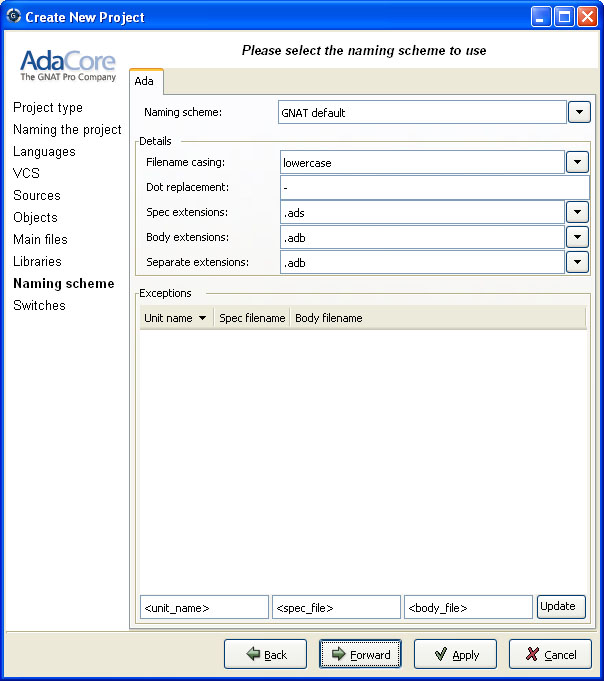
\includegraphics{naming-scheme.jpg}

For all languages, GPS accepts exceptions to this standard naming scheme. For
instance, this let you specify that in addition to using \code{.adb} for Ada
body files, the file \code{foo.ada} should also be considered as an Ada file.

The list of exceptions is displayed in the bottom list of the naming scheme
editor. To remove entries from this list, select the line you want to remove,
and then press the \code{Del} key.  The contents of the lines can be edited
interactively, by double-clicking on the line and column you want to edit.

To add new entries to this list, use the fields at the bottom of the window,
and press the update button.

\index{multi-unit source files}
GNAT and GPS both support Ada source files that contain multiple Ada units
(typically a single file would contain both the spec and the body of the unit
for instance). This is not a recommend approach if you can avoid it, since that
might trigger unnecessary recompilation of your source files. Such source files
are always handled as naming scheme exceptions, and you can specify those in
the editor by adding ``at 1'', ``at 2'',... after the file name for either the
spec, the body or both. The digit after ``at'' is the index (starting at 1) of
the unit in the source file.

For instance, specifying ``file.ada at 1'' for the spec and ``file.ada at 2'' for
the body of the unit ``unit'' indicates that the two components of the unit are
in the same file, first the spec, followed by the body.


\subsection{Switches}
\label{projects:switches}\phantomsection\label{projects:id10}
\index{switches}
The last page of the project wizard is used to select the default switches to
be used by the various tools that GPS calls (compiler, linker, binder, pretty
printer, ...).

\index{screen shot}
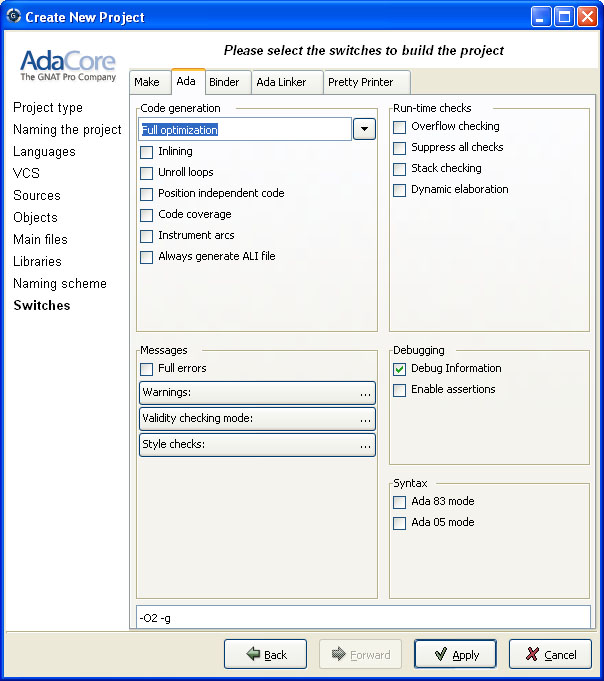
\includegraphics{switch-editor.jpg}

This page appears as a notebook, where each page is associated with a specific
tool. All these pages have the same structure:
\begin{description}
\item[{\emph{Graphical selection of switches}}] \leavevmode
The top part of each page contains a set of buttons, combo boxes,
entry fields, ... which give fast and intuitive access to the most
commonly used switches for that tool.

\item[{\emph{Textual selection of switches}}] \leavevmode
The bottom part is an editable entry field, where you can directly
type the switches. This makes it easier to move from
an older setup (e.g. Makefile, script) to GPS, by copy-pasting switches.

\end{description}

The two parts of the pages are kept synchronized at any time: clicking on a
button will edit the entry field to show the new switch; adding a new switch by
hand in the entry field will activate the corresponding button if there is one.

Any switch can be added to the entry field, even if there is no corresponding
button. In this case, GPS will simply forward it to the tool when it is called,
without trying to represent it graphically.


\section{The Project Dependencies Editor}
\label{projects:id11}\label{projects:the-project-dependencies-editor}
\index{project dependencies}
You can edit the dependencies between projects through the contextual menu
\emph{Project-\textgreater{}Dependencies...} in the Project View.

This view makes it easy to indicate that your project depends on external
libraries, or other modules in your source code. For instance, you can give
access to the GtkAda graphical library in your project by adding a project
dependency to gtkada.gpr, assuming GtkAda has been installed in your system.

The dependencies also determine in what order your application is built.  When
you compile a project, the builder will first make sure that the projects it
depends on are up-to-date, and otherwise recompile them.

\index{screen shot}
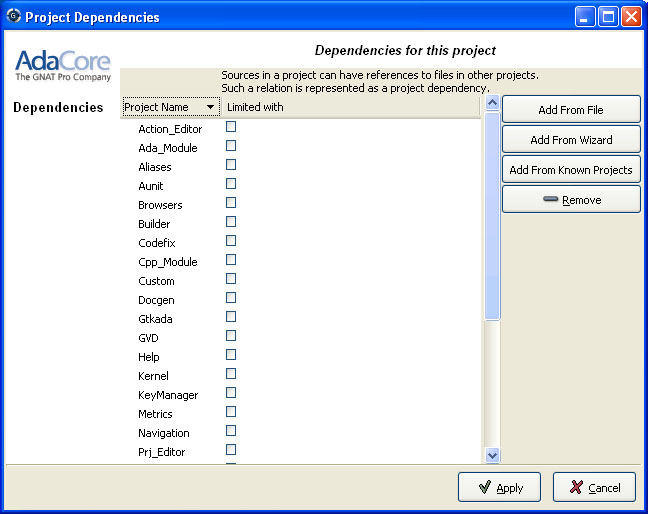
\includegraphics{project-deps.jpg}

When you select that contextual menu, GPS will open a dialog that allows you to
add or remove dependencies to your project. New dependencies are added by
selecting a project file name from one of several sources:
\begin{itemize}
\item {} 
One of the loaded project from the current project tree

\item {} 
One of the predefined projects

These are the projects that are found in one of the directories referenced in
the \emph{ADA\_PROJECT\_PATH} environment variable. Typically, these include third
party libraries, such as GtkAda, win32ada, ...

\item {} 
A new project created through the project wizard

\item {} 
Any project file located on the disk

\end{itemize}

In all these cases, you will generally be able to choose whether this should be
a simple dependency, or a limited dependency. The latter allows you to have
mutually dependent projects (A depends on B, which in turns depends on A even
indirectly), although you cannot reference the attribute of such a project in
the current project (for instance to indicate that the compiler switches to use
for A are the same as for B -- you need to duplicate that information).

In some cases, GPS will force a limited dependency on you to avoid loops in the
dependencies that would make the project tree illegal.


\section{The Project Properties Editor}
\label{projects:the-project-properties-editor}\label{projects:id12}
\index{project properties editor}
The project properties editor gives you access at any time to the properties of
your project. It is accessible through the menu \emph{Project-\textgreater{}Edit Project
Properties}, and through the contextual menu \emph{Edit project properties} on any
project item, e.g. from the Project View or the Project Browser.

If there was an error loading the project (invalid syntax, non-existing
directories, ...), a warning dialog is displayed when you select the menu. This
reminds you that the project might be only partially loaded, and editing it
might result in the loss of data. In such cases, it is recommended that you
edit the project file manually, which you can do directly from the pop-up
dialog.

Fix the project file as you would for any text file, and then reload it
manually (through the \emph{Project-\textgreater{}Open...} or \emph{Project-\textgreater{}Recent} menus.

\index{screen shot}
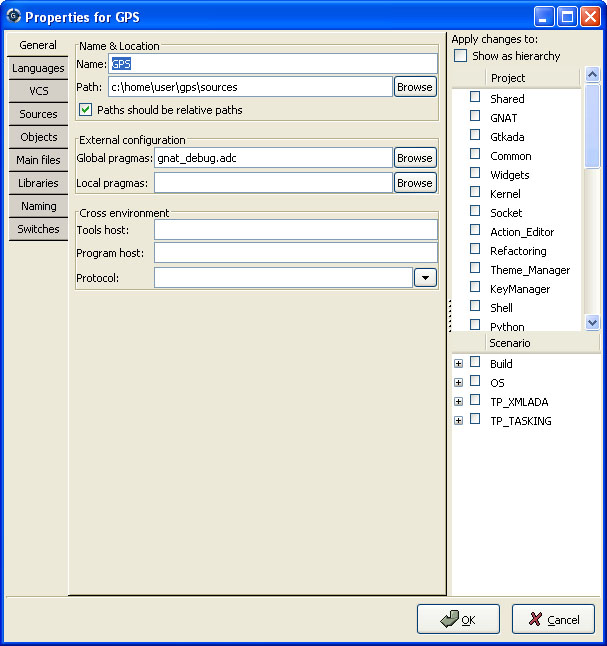
\includegraphics{project-properties.jpg}

The project properties editor is divided in three parts:

\emph{The attributes editor}
\begin{quote}

The contents of this editor are very similar to that of the project wizard
({\hyperref[projects:the-project-wizard]{\emph{The Project Wizard}}}). In fact, all pages but the \emph{General} page are
exactly the same, and you should therefore read the description for these in
the project wizard chapter.

See also {\hyperref[cross_env:working-in-a-cross-environment]{\emph{Working in a Cross Environment}}} for more info on the \emph{Cross
environment} attributes.
\end{quote}

\emph{The project selector}
\begin{quote}

This area, in the top-right corner of the properties editor, contains a list
of all the projects in the hierarchy. The value in the attributes editor is
applied to all the selected projects in this selector. You cannot unselect
the project for which you activated the contextual menu.

Clicking on the right title bar (\emph{Project}) of this selector will sort the
projects in ascending or descending order.

Clicking on the left title bar (untitled) will select or unselect all the
projects.

This selector has two different possible presentations, chosen by the toggle
button on top: you can either get a sorted list of all the projects, each one
appearing only once. Or you can have the same project hierarchy as displayed
in the project view.
\end{quote}

\emph{The scenario selector}
\begin{quote}

This area, in the bottom-right corner of the properties editor, lists all the
scenario variables declared for the project hierarchy. By selecting some or
all of their values, you can chose to which scenario the modifications in the
attributes editor apply.

Clicking on the left title bar (untitled, on the left of the \emph{Scenario}
label) will select or unselect all values of all variables.

To select all values of a given variable, click on the corresponding check
button.
\end{quote}


\section{The Switches Editor}
\label{projects:id13}\label{projects:the-switches-editor}
\index{switches editor}
The switches editor, available through the menu \emph{Project-\textgreater{}Edit Switches}, lists
all the source files associated with the selected project.

For each file, the compiler switches are listed. These switches are displayed
in gray if they are the default switches defined at the project level
({\hyperref[projects:the-project-properties-editor]{\emph{The Project Properties Editor}}}). They are defined in black if they are
specific to a given file.

Double-clicking in the switches column allows you to edit the switches for a
specific file. It is possible to edit the switches for multiple files at the
same time by selecting them before displaying the contextual menu (\emph{Edit
switches for all selected files}).

When you double-click in one of the columns that contain the switches, a new
dialog is opened that allows you to edit the switches specific to the selected
files.

This dialog has a button titled \emph{Revert}. Clicking on this button will cancel
any file-specific switch, and revert to the default switches defined at the
project level.

\index{screen shot}
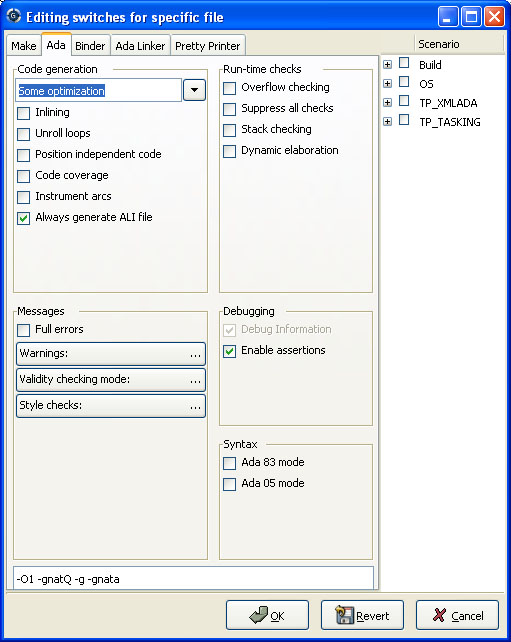
\includegraphics{switch-editor-revert.jpg}


\section{The Project Browser}
\label{projects:the-project-browser}\label{projects:id14}
\index{project browser}
The project graph is a special kind of browser ({\hyperref[browsing:source-browsing]{\emph{Source Browsing}}}). It
shows the dependencies between all the project in the project hierarchy. Two
items in this browser will be linked if one of them imports the other.

\index{examine projects imported by}
It is accessed through the contextual menu in the project view, by selecting
the \emph{Show projects imported by...} item, when right-clicking on a project node.

Clicking on the left arrow in the title bar of the items will display all the
projects that import that project. Similarly, clicking on the right arrow will
display all the projects that are imported by that project.

The contextual menu obtained by right-clicking on a project item contains
several items. Most of them are added by the project editor, and gives direct
access to editing the properties of the project, adding dependencies...
{\hyperref[projects:the-project-view]{\emph{The Project View}}}.

\index{screen shot}
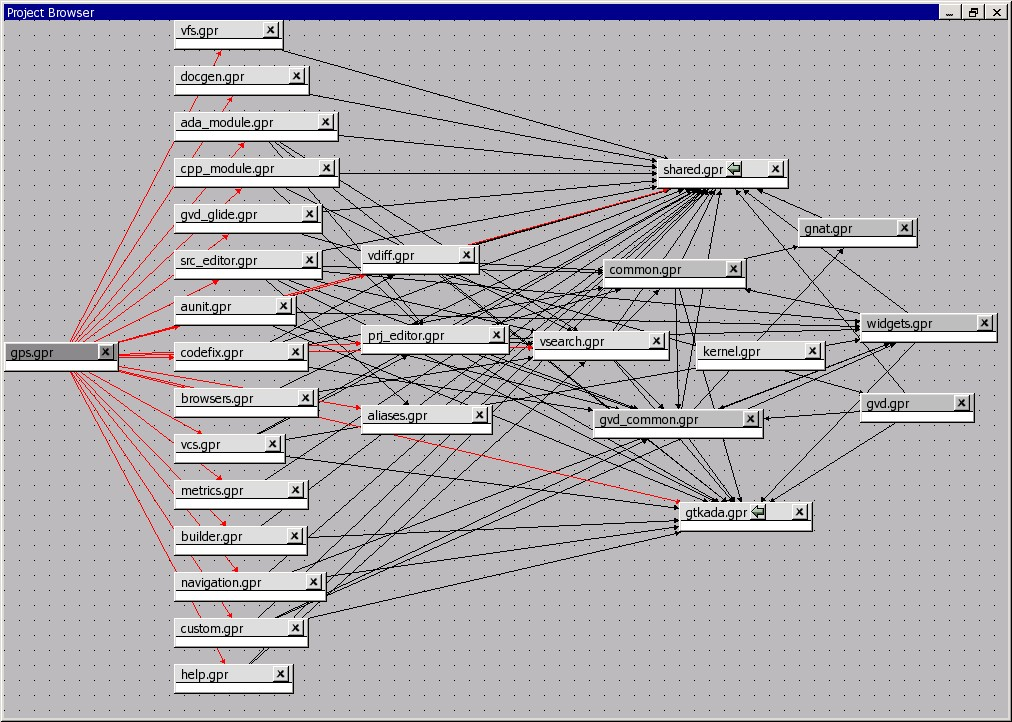
\includegraphics{project-browser.jpg}

Some new items are added to the menu:
\begin{description}
\item[{\emph{Locate in Project View}}] \leavevmode
\index{locate in Project View}
Selecting this item will switch the focus to the project view, and highlight
the first project node found that matches the project in the browser item.
This is a convenient way to get information like the list of directories or
source files for that project.

\item[{\emph{Show dependencies}}] \leavevmode
\index{show dependencies}
This item plays the same role as the right arrow in the title bar, and
display all the projects in the hierarchy that are imported directly by the
selected project

\item[{\emph{Show recursive dependencies}}] \leavevmode
\index{show recursive dependencies}
This item will display all the dependencies recursively for the project (i.e.
the projects it imports directly, the projects that are imported by them, and
so on).

\item[{\emph{Show projects depending on}}] \leavevmode
\index{show projects depending on}
This item plays the same role as the left arrow in the title bar, and
displays all the projects that directly import the selected project.

\end{description}


\chapter{Searching and Replacing}
\label{searching::doc}\label{searching:searching-and-replacing}\label{searching:id1}
\index{find}
\index{search}
\index{replace}
GPS provides extensive search capabilities among its different elements. For
instance, it is possible to search in the currently edited source file, or in
all the source files belonging to the project, even those that are not
currently open. It is also possible to search in the project view (on the left
side of the main GPS window), ...

\index{project view}
\index{menu}
\index{key}
\index{search context}
All these search contexts are grouped into a single graphical window, that you
can open either through the menu \emph{Navigate-\textgreater{}Find/Replace...}, or the shortcut
\code{Ctrl-F}.

By default, the search window is floating, ie appears as a dialog on top of
GPS. You can choose to put it inside the multiple document interface
permanently for easier access. This can be done by selecting the menu
\emph{Window-\textgreater{}Floating}, and then drag-and-dropping the search window in a new
location if you wish (for instance above the Project View).

Selecting either of these two options will pop up a dialog on the screen,
similar to the following:

\index{screen shot}
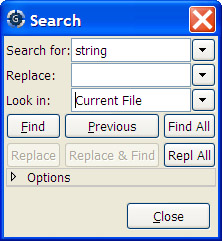
\includegraphics{search-hide.jpg}

On this screen shot, you can see three entry fields:
\begin{description}
\item[{\emph{Search for}}] \leavevmode
\index{search for}
This is the location where you type the string or pattern you are looking
for. The search widget supports two modes, either fixed strings or regular
expressions. You can commute between the two modes by either clicking on the
\emph{Options} button and selecting the appropriate check box, or by opening the
combo box (click on the arrow on the right of the entry field).

In this combo box, a number of predefined patterns are provided. The top two
ones are empty patterns, that automatically set up the appropriate fixed
strings/regular expression mode. The other regular expressions are
language-specific, and will match patterns like Ada type definition, C++
method declaration, ...

\index{C++}
\index{Ada}
\item[{\emph{Replace with}}] \leavevmode
\index{replace with}
This field should contain the string that will replace the occurrences of the
pattern defined above.  The combo box provides a history of previously used
replacement strings. If regular expression is used for search, special
escapes 1, 2 .. 9 in this field refer to the corresponding matching
sub-expressions and 0 refers whole matched string.

\item[{\emph{Look in}}] \leavevmode
\index{look in}
This field defines the context in which the search should occur.

\index{search context}
GPS will automatically select the most appropriate context when you open the
search dialog, depending on which component currently has the focus. If
several contexts are possible for one component (for example, the editor has
``Current\_File'', ``Files from Project'', ``Files...'' and ``Open Files''), then the
last one you've been using will be selected. You can of course change the
context to another one if needed.

Clicking on the arrow on the right will display the list of all possible
contexts. This list includes:
\begin{description}
\item[{\emph{Project View}}] \leavevmode
Search in the project view. An extra \emph{Scope} box will be displayed
where you can specify the scope of your search, which can be a set of:
\emph{Projects, Directories, Files, Entities}. The search in entities
may take a long time, search each file is parsed during the search.

\item[{\emph{Open Files}}] \leavevmode
Search in all the files that are currently open in the source editor. The
\emph{Scope} entry is described in the \emph{Files...} section below.

\end{description}

\emph{Files...}
\begin{quote}

Search in a given set of files. An extra \emph{Files} box will be displayed
where you can specify the files by using standard shell (Unix or Windows)
regular expression, e.g. \emph{*.ad?} for all files ending with .ad and any
trailing character. The directory specified where the search starts, and
the \emph{Recursive search} button whether sub directories will be searched as
well.

The \emph{Scope} entry is used to restrict the search to a set of language
constructs, e.g. to avoid matching on comments when you are only interested
in actual code, or to only search strings and comments, and ignore the
code.
\end{quote}

\emph{Files From Project}
\begin{quote}

Search in all the files from the project, including files from project
dependencies. The \emph{Scope} entry is described in the \emph{Files...} section
above.
\end{quote}

\emph{Files From Current Project}
\begin{quote}

Search in all the files from the currently selected project, defaulting on
the root project if there is no project currently selected.
The \emph{Scope} entry is described in the \emph{Files...} section above.
\end{quote}

\emph{Files From Runtime}
\begin{quote}

Search in all specification files from GNAT runtime library.
The \emph{Scope} entry is described in the \emph{Files...} section above.
\end{quote}

\emph{Current File}
\begin{quote}

Search in the current source editor.  The \emph{Scope} entry is described in the
\emph{Files...} section above.
\end{quote}

\emph{Project Browser}
\begin{quote}

Search in the project browser ({\hyperref[projects:the-project-browser]{\emph{The Project Browser}}}).
\end{quote}

The default value for \emph{Look In} is set through various means: by default, GPS
will select a context that matches the currently selected window. For
instance, if you are in an editor and open the search dialog, the context
will be set to \emph{Current File}. But if the project view is the active window,
the context will be set to \emph{Project View}.  Optionally, GPS can remember the
last context that was set (see the preference \emph{Search/Preserve Search
Context}. If this is set, and an editor is selected, GPS will remember
whether the last time you started a search from an editor you decided to
search in \emph{Current File} or \emph{Files From Project} for instance.

Finally, you can create key shortcuts (through the \emph{/Edit/Key Shortcuts}
menu, in the \emph{Search} category) to open the search dialog and set the context
to a specific value.

\end{description}

The second part of the window is a row of buttons, to start the search (or
continue to the next occurrence), and to display the options.

\index{screen shot}
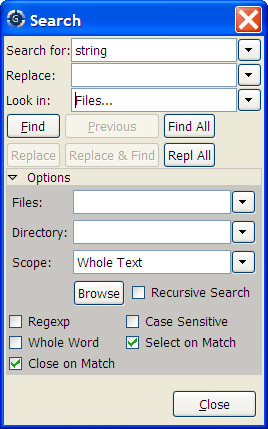
\includegraphics{search-options.jpg}

There are five check boxes in this options box.
\begin{description}
\item[{\emph{{}`''Regexp''{}`}}] \leavevmode
\index{regular expression}
This button commutes between fixed string patterns and regular expressions.
You can also commute between these two modes by selecting the arrow on the
right of the \emph{Search for:} field.  The grammar followed by the regular
expressions is similar to the Perl and Python regular expressions grammar,
and is documented in the GNAT run time file \code{g-regpat.ads}. To open it
from GPS, you can use the {\hyperref[editing:open-from-project]{\emph{open from project}}} dialog
(\emph{File-\textgreater{}Open From Project...}) and type g-regpat.ads.

\item[{\emph{{}`''Whole Word''{}`}}] \leavevmode
\index{whole word}
If activated, this check box will force the search engine to ignore
substrings. ``sensitive'' will no longer match ``insensitive''.

\item[{\emph{{}`Select on Match{}`}}] \leavevmode
\index{select window on match}
When this button is selected, the focus is given to the editor that contains
the match, so that you can start editing the text immediatly. If the button
is not selected, the focus is left on the search window, so that you can
press Enter to search for the next occurrence.

\item[{\emph{{}`Close on Match{}`}}] \leavevmode
\index{close dialog on match}
This button only appears if the search window is floating. If this button is
enabled, the search window will be automatically closed when an occurrence of
the search string is found.

\item[{\emph{{}`''Case Sensitive Search''{}`}}] \leavevmode
\index{case sensitive}
By default, patterns are case insensitive (upper-case letters and lower-case
letters are considered as equivalent). You can change this behavior by
clicking on this check box.

\item[{\emph{{}`''Case Preserving Replace''{}`}}] \leavevmode
\index{case preserving}
When this is checked, replacements preserve casing. Three casings are
detected and preserved: all lower, all UPPER, and Mixed\_Case where the first
character of each word is capitalized. Note that when the replace pattern is
not all lower case, replacement is never case-preserving, the original casing
of the replace pattern is used.

\end{description}

Pressing the \emph{Find} / \emph{Previous} buttons performs an interactive search.  It
stops as soon as one occurrence of the pattern is found.  search. Once a first
occurrence has been found, the \emph{Find} button is renamed to \emph{Next}.  You then
have to press the \emph{Next} button (or the equivalent shortcut \code{Ctrl-N}) to
go to the next occurrence.

If you use the \emph{Find all} button, the search widget will start searching for
all occurrences right away, and put the results in a new window called
\emph{Locations}, {\hyperref[main_window:the-locations-view]{\emph{The Locations View}}}.

The \emph{Replace} and \emph{Replace \& Find} buttons are grayed out as long as no
occurence of the pattern is found. In order to enable them, you have to start a
search, e.g. by pressing the \emph{Find} button. Pressing \emph{Replace} will replace the
current occurence (and therefore the two buttons will be grayed out), and
\emph{Replace \& Find} will replace the occurence and then jump to the next one, if
any. If you don't want to replace the current occurence, you can jump directly
to the next one by pressing \emph{Next}.

The \emph{Repl all} button will replace all the occurences found. By default, a
popup is displayed and ask for confirmation. It's possible to disable this
popup by either checking the box ``Do not ask this question again'', or by going
in the Search pannel of the preferences pages, and unchecking ``Confirmation for
`Replace all'''. The confirmation popup can be reenabled through this checkbox.

\index{MDI}
\index{Multiple Document Interface}
As most GPS components, the search window is under control of the multiple
document interface, and can thus be integrated into the main GPS window instead
of being an external window.

\index{menu}
To force this behavior, open the menu \emph{Window}, select \emph{Search} in the list at
the bottom of the menu, and then select either \emph{Floating} or \emph{Docked}.

If you save the desktop (\emph{File-\textgreater{}Save More-\textgreater{}Desktop}, GPS will automatically
reopen the search dialog in its new place when it is started next time.


\chapter{Compilation/Build}
\label{compilation:id1}\label{compilation::doc}\label{compilation:compilation-build}
\index{compilation}
\index{build}
This chapter describes how to compile files, build executables and run them.
Most capabilities can be accessed through the \emph{Build} menu item, or through the
\emph{Build} and \emph{Run} contextual menu items, as described in the following section.

When compiler messages are detected by GPS, an entry is added in the \emph{Locations
View}, allowing you to easily navigate through the compiler messages (see
{\hyperref[main_window:the-locations-view]{\emph{The Locations View}}}), or even to automatically correct some errors or
warnings (see {\hyperref[tools:code-fixing]{\emph{Code Fixing}}}).

Compiler messages also appear as icons on the side of lines in the source
editors. When the mouse pointer is left on these icons, a tooltip appears,
listing the error messages found on this line. When GPS is capable of
automatically correcting the errors, clicking on the icon will apply the fix to
the source code. The icons on the side of editors are removed when the
corresponding entries are removed from {\hyperref[main_window:the-locations-view]{\emph{The Locations View}}}.


\section{The Build Menu}
\label{compilation:the-build-menu}\label{compilation:id2}
The build menu gives access to capabilities related to checking, parsing and
compiling files, as well as creating and running executables.  note that this
menu is fully configurable via the \emph{Targets} dialog, so what is documented in
this manual are the default menus.

See {\hyperref[compilation:the-target-configuration-dialog]{\emph{The Target Configuration Dialog}}}.
\begin{description}
\item[{\emph{Check Syntax}}] \leavevmode
Check the syntax of the current source file. Display an error message in
the \emph{Messages} window if no file is currently selected.

\item[{\emph{Check Semantic}}] \leavevmode
Check the semantic of the current source file. Display an error message in
the \emph{Messages} window if no file is currently selected.

\end{description}

\emph{Compile File}
\begin{quote}

Compile the current file.

By default, will display an intermediate dialog where you can add extra
switches, or simply press \code{Enter} to get the standard (or previous)
switches.  Display an error message in the \emph{Messages} window if no file is
selected.

If errors or warnings occur during the compilation, the corresponding
locations will appear in the Locations View. If the corresponding Preference
is set, the source lines will be highlighted in the editors (see
{\hyperref[extending:the-preferences-dialog]{\emph{The Preferences Dialog}}}).  To remove the highlighting on these lines,
remove the files from the Locations View using either the contextual menu
(\emph{Remove category}) or by closing the Locations View.
\end{quote}

\emph{Project}
\begin{quote}
\begin{description}
\item[{\emph{Build \textless{}main\textgreater{}}}] \leavevmode
The menu will list of all mains defined in your project hierarchy.
Each menu item will build the selected main.

\end{description}

\emph{Build All}
\begin{quote}

Build and link all main units defined in your project.  If no main unit is
specified in your project, build all files defined in your project and
subprojects recursively.  For a library project file, compile sources and
recreate the library when needed.
\end{quote}

\emph{Compile All Sources}
\begin{quote}

Compile all source files defined in the top level project.
\end{quote}

\emph{Build \textless{}current file\textgreater{}}
\begin{quote}

Consider the currently selected file as a main file, and build it.
\end{quote}

\emph{Custom Build...}
\begin{quote}

Display a text entry where you can enter any external command. This menu is
very useful when you already have existing build scripts, make files, ...
and want to invoke them from GPS. If the \emph{SHELL} environment variable is
defined (to e.g. \emph{/bin/sh}), then the syntax used to execute the command is
the one for this shell. Otherwise, the command will be spawned directly by
GPS without any shell interpretation.
\end{quote}
\end{quote}

\emph{Clean}
\begin{quote}

\emph{Clean All}
\begin{quote}

Remove all object files and other compilation artifacts associated to all
projects related to the current one. It allows to restart a complete build
from scratch.
\end{quote}

\emph{Clean Root}
\begin{quote}

Remove all object files and other compilation artifacts associated to the
root project. It does not clean objects from other related projects.
\end{quote}
\end{quote}

\emph{Makefile}
\begin{quote}

If you have the \emph{make} utility in your PATH, and have a file called
\code{Makefile} in the same directory as your project file is, or if you've
set the \emph{makefile} property in the \emph{Make} section of the project properties
(see {\hyperref[projects:the-project-properties-editor]{\emph{The Project Properties Editor}}}), this menu will be displayed,
giving access to all the targets defined in your makefile.
\end{quote}

\emph{Ant}
\begin{quote}

If you have the \emph{ant} utility in your PATH, and have a file called
\code{build.xml} in the same directory as your project file is, or if you've
set the \emph{antfile} property in the \emph{Ant} section of the project properties
(see {\hyperref[projects:the-project-properties-editor]{\emph{The Project Properties Editor}}}), this menu will be displayed,
giving access to all the targets defined in your ant file.
\end{quote}

\emph{Run}
\begin{quote}

\emph{main}
\begin{quote}

For each main source file defined in your top level project, an entry is
listed to run the executable associated with this main file.  Running an
application will first open a dialog where you can specify command line
arguments to your application, if needed. You can also specify whether the
application should be run within GPS (the default), or using an external
terminal.

When running an application from GPS, a new execution window is added in
the bottom area where input and output of the application is handled. This
window is never closed automatically, even when the application terminates,
so that you can still have access to the application's output. If you
explicitly close an execution window while an application is still running,
a dialog window will be displayed to confirm whether the application should
be terminated.

When using an external terminal, GPS launches an external terminal utility
that will take care of the execution and input/output of your application.
This external utility can be configured in the preferences dialog
(\emph{External Commands-\textgreater{}Execute command}).

The GPS execution windows have several limitations compared to external
terminals. In particular, they do not handle signals like \code{ctrl-z} and
\code{control-c}. In general, if you are running an interactive
application, we strongly encourage you to run in an external terminal.

Similarly, the \emph{Run} contextual menu accessible from a project entity
contains the same entries.
\end{quote}

\emph{Custom...}
\begin{quote}

Similar to the entry above, except that you can run any arbitrary
executable.  If the \emph{SHELL} environment variable is defined (to e.g.
\emph{/bin/sh}), then the syntax used to execute the command is the one for this
shell. Otherwise, the command will be spawned directly by GPS without any
shell interpretation.
\end{quote}
\end{quote}
\begin{description}
\item[{\emph{Recompute Xref info}}] \leavevmode
\index{C}
\index{C++}
Recompute the cross-reference information for Ada, C and C++ source files.
{\hyperref[navigation:support-for-cross-references]{\emph{Support for Cross-References}}}.

\item[{\emph{Load xref info in memory}}] \leavevmode
\index{C}
\index{C++}
Load all the cross-reference information in memory. This menu is generally
not needed, {\hyperref[navigation:support-for-cross-references]{\emph{Support for Cross-References}}}.

\end{description}

\emph{Settings}
\begin{quote}

\emph{Targets}
\begin{quote}

\index{Targets}
This opens the Target Configuration Dialog.
{\hyperref[compilation:the-target-configuration-dialog]{\emph{The Target Configuration Dialog}}}.
\end{quote}

\emph{Toolchains}
\begin{quote}

\index{Toolchains}
Open a dialog allowing the configuration of GPS for working with two
compilation toolchains. This is particulary useful when compiling a project
with an old compiler, while wanting up-to-date functionalities from the
associated tools (gnatmetric, gnatcheck and so on).
{\hyperref[compilation:working-with-two-compilers]{\emph{Working with two compilers}}}.
\end{quote}
\end{quote}

The \emph{Tools-\textgreater{}Interrupt} menu can be used to interrupt the last compilation or
run command. Once you have interrupted that last operation, you can interrupt
the previous one by selecting the same menu again.

However, the easiest way to interrupt a specific operation, no matter if it was
started last or not, is to use the \emph{Task Manager}, through the
\emph{Tools-\textgreater{}Views-\textgreater{}Tasks} menu. It will show one line per running process, and
right-clicking on any of these lines gives the possibility to interrupt that
process.

If your application is build through a Makefile, you should probably load the
\code{Makefile.py} startup script (see the menu \emph{/Tools/Plug-ins}).


\section{The Target Configuration Dialog}
\label{compilation:id3}\label{compilation:the-target-configuration-dialog}
\index{Targets}
GPS provides an interface for launching operations like building projects,
compiling individual files, performing syntax or semantic checks, and so on.
All these operations have in common that they involve launching an external
command, and parsing the output for error messages. In GPS, these operations
are called ``Targets'', and can be configured either through the Target
Configuration dialog, or through XML configuration.
{\hyperref[extending:customizing-build-targets-and-models]{\emph{Customizing build Targets and Models}}}.

\index{screen shot}
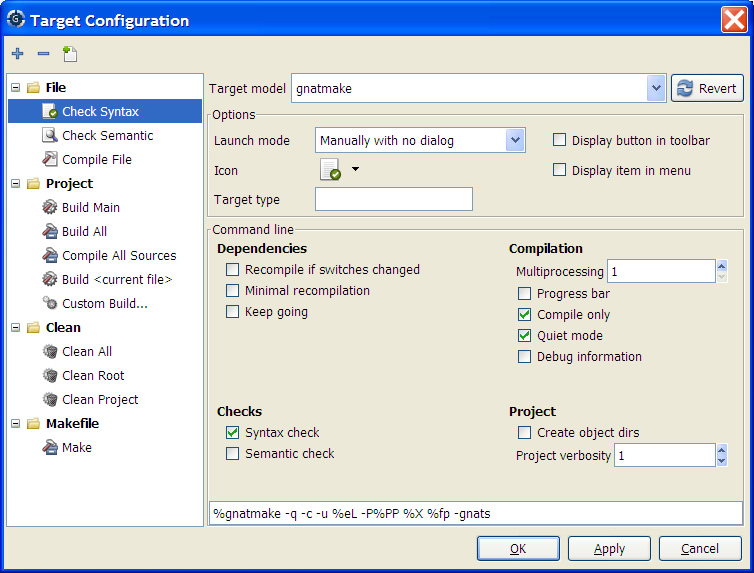
\includegraphics{target-configuration-dialog.jpg}

This dialog is divided in two areas: on the left, a tree listing Targets, and,
in the main area, a panel for configuring the Target which is currently
selected in the tree.


\subsection{The Targets tree}
\label{compilation:the-targets-tree}
The Tree contains a list of targets, organized by categories.

On top of the tree are three buttons:
\begin{itemize}
\item {} 
The Add button creates a new target.

\item {} 
The Remove button removes the currently selected target. Note that only
user-defined targets can be removed, the default targets created by GPS cannot
be removed.

\item {} 
The Clone button creates a new user-defined target which is identical
to the currently selected target.

\end{itemize}


\subsection{The configuration panel}
\label{compilation:the-configuration-panel}
On top of the configuration panel, one can select the Target model.  The Model
determines the graphical options available in the ``Command line'' frame.

The ``Revert'' button resets all target settings to their original value.

The ``Options'' frame contains a number of options that are available for all
Targets.
\begin{itemize}
\item {} 
The Launch mode indicates the way the target is launched:
\begin{itemize}
\item {} 
Manually:
the target is launched when clicking on the corresponding icon
in the toolbar, or when activating the corresponding menu item.
In the latter case, a dialog is displayed, allowing last-minute
modifications of the command line.

\item {} 
Manually with dialog:
same as Manually, but the dialog is always displayed, even when
clicking on the toolbar icon.

\item {} 
Manually with no dialog:
same as Manually, but the dialog is never displayed, even when
activating the menu item.

\item {} 
On file save:
the Target is launched automatically by GPS when a file is saved.
The dialog is never displayed.

\item {} 
In background:
the Target is launched automatically in the background after each
modification in the source editor. See \emph{Background compilations}
below.

\end{itemize}

\item {} 
Icon: the icon to use for representing this target in the menus and in the
toolbar. To use one of your icons, you must register a icons using the
\emph{\textless{}stock\textgreater{}} XML customization node. ({\hyperref[extending:adding-stock-icons]{\emph{Adding stock icons}}}). Then, use
``custom'' choice and enter in the text field the ID of the icon.

\item {} 
Target type: type of target described. If empty, or set to \emph{Normal},
represents a simple target. If set to another value, represents multiple
subtargets.  For example, if set to \emph{main}, each subtarget corresponds to a
Main source as defined in the currently loaded project.  Other custom values
may be defined, and then handled via the \emph{compute\_build\_targets} hook.

\end{itemize}

The ``Display'' frame indicates where the launcher for this target should be
visible.
\begin{itemize}
\item {} 
in the toolbar: when active, a button is displayed in the main toolbar,
allowing to quickly launch a Target.

\item {} 
in the main menu: whether to display a menu item corresponding to the Target
in the main GPS menu. By default, Targets in the ``File'' category are listed
directly in the Build menu, and Targets in other categories are listed in a
submenu corresponding to the name of the category.

\item {} 
in contextual menus for projects: whether to display an item in the
contextual menu for projects in the Project View

\item {} 
in contextual menus for files: whether to display an item in the contextual
menus for files, for instance in file items in the Project View or directly
on source file editors.

\end{itemize}

The ``Command line'' contains a graphical interface for some configurable
elements of the Target, which are specific to the Model of this Target.

The full command line is displayed at the bottom. Note that it may contain
Macro Arguments. For instance if the command line contains the string ``\%PP'',
GPS will expand this to the full path to the current project. For a full list
of available Macros, see {\hyperref[extending:macro-arguments]{\emph{Macro arguments}}}.


\subsection{Background compilations}
\label{compilation:background-compilations}
GPS is capable of launching compilation targets in the background. This means
that GPS will launch the compiler on the current state of the file in the
editor.

Error messages resulting from background compilations are not listed in the
Locations view or the Messages window. The full messages are listed in the
Background Build console, accessible from the menu \emph{Tools-\textgreater{}Console}.  Error
messages which contain a source location indication are shown as icons on the
side of lines in editors, and the exact location is highlighted directly in the
editor. On both of these places, tooltips show the contents of the error
messages.

Messages from background compilations are removed automatically either when a
new background compilation has finished, or when a non-background compilation
is launched.

GPS will launch background compilations for all targets that have a \emph{Launch
mode} set to \emph{In background}, after modifications occur in a source editor.
Background compilation is useful mostly for targets such as \emph{Compile File} or
\emph{Check Syntax}. For targets that work on Mains, the last main that was used in
a non-background is considered, defaulting to the first main defined in the
project hierarchy.

Background compilations are not launched while GPS is already listing results
from non-background compilations, ie as long as there are entries in the
Locations View showing entries in the \emph{Builder results} category.


\section{The Build Mode}
\label{compilation:the-build-mode}\label{compilation:id4}
\index{Mode}
GPS provides an easy way to build your project with different options, through
the Mode selection, located in the main toolbar.

When the Mode selection is set to \emph{default}, the build is done using the
switches defined in the project. When the Mode selection is set to another
value, then specialized parameters are passed to the builder. For instance, the
\emph{gcov} Mode adds all the compilation parameters needed to instrument the
produced objects and executables to work with the \emph{gcov} tool.

In addition to changing the build parameters, the Mode selection has the effect
of changing the output directory for objects and executables. For instance,
objects produced under the \emph{debug} mode will be located in the \emph{debug}
subdirectories of the object directories defined by the project.  This allows
switching from one Mode to another without having to erase the objects
pertaining to a different Mode.

It is possible to define new Modes using XML customization, see
{\hyperref[extending:customizing-build-targets-and-models]{\emph{Customizing build Targets and Models}}}.

Note that the Build Mode affects only builds done using recent versions of
gnatmake and gprbuild. The Mode selection has no effect on builds done through
Targets that launch other builders.


\section{Working with two compilers}
\label{compilation:id5}\label{compilation:working-with-two-compilers}
\index{Toolchains}
This functionality is intended for people whose projects need to be compiled
with a specific (old) version of the GNAT toolchain, while still desiring to
take full advantage of up-to-date associated tools for non-compilation actions,
such as checking the code against a coding standard, getting better
cross-reference browsing in GPS, computing metrics and so on.

GPS now allows you to handle this case. To configure GPS to make it handle two
compiler toolchains, you need to use the \emph{Build-\textgreater{}Settings-\textgreater{}Toolchains} menu.
This will open a dialog where you can activate the multiple-toolchains mode.

\index{screen shot}
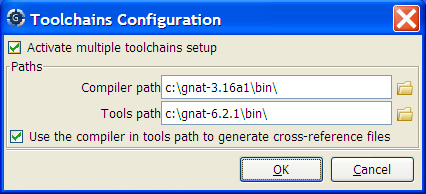
\includegraphics{toolchains-config.jpg}

In this dialog, two paths need to be configured: the compiler path and the
tools path. The first one is used to actually compile the code, while the
second one is used to run up-to-date tools to get more functionalities or
accurate results.

Note that GPS will only enable the \emph{OK} button when the two paths are set to
different location, since otherwise it does not make sense to enable the
multiple toolchains set up.

From this dialog, you can also activate an automated cross-reference
generation. The cross-reference files are the .ali files generated by the GNAT
compiler together with the compiled object. Those files are used by GPS for
several functionalities, such as cross-reference browsing or documentation
generation. Having those .ali files produced by a recent compiler helps having
more accurate results with those functionalities, but might interract badly
with an old compiler also reading those .ali files for compiling a project.

If the automated xref generation is activated, then GPS will generate those
.ali files using the compiler found in the tools path, and place them in a
directory distinct from the one used by the actual compiler. This allows GPS to
take full benefit of up-to-date cross-reference files, while keeping the old
toolchain happy as its .ali files remain untouched.

Note that the cross-reference files generation does not output anything in the
``Messages'' window, so as to not confuse the output of the regular build
process. If needed, you can see the output of the cross-ref generation command
by selecting the \emph{Tools-\textgreater{}Consoles-\textgreater{}Auxiliary Builds} menu.


\subsection{Interaction with the remote mode}
\label{compilation:interaction-with-the-remote-mode}
The ability to work with two compilers has impacts on the remote mode
configuration: paths defined here are local paths, so they have no meaning on
the server side.

To handle the case of using a specific compiler version on the remote side
while still wanting up-to-date tools, the following behavior is applied when
both a remote compilation server is defined, and the multiple toolchains mode
is activated:
\begin{itemize}
\item {} 
The compiler path is ignored when a remote build server is defined. All
compilation actions are then performed normally on the build server.

\item {} 
The tools path is however taken into account, and all related actions
are performed on the local machine using this path.

\item {} 
The cross-reference files are taken care of by the rsync mechanism
so that they don't get overwritten during local and remote host
synchronisations, as build and cross-reference generation actions occur at
the same time, on the local machine and on the distant server.

\end{itemize}


\chapter{Source Browsing}
\label{browsing:source-browsing}\label{browsing::doc}\label{browsing:id1}
\index{source browsing}

\section{General Issues}
\label{browsing:id2}\label{browsing:general-issues}\label{browsing:index-0}
GPS contains several kinds of browsers, that have a common set of basic
functionalities. There are currently four such browsers: the project browser
({\hyperref[projects:the-project-browser]{\emph{The Project Browser}}}), the call graph ({\hyperref[browsing:call-graph]{\emph{Call Graph}}}), the
dependency browser ({\hyperref[browsing:dependency-browser]{\emph{Dependency Browser}}}) and the entity browser
({\hyperref[browsing:entity-browser]{\emph{Entity Browser}}}).

All these browsers are interactive viewers. They contain a number of items,
whose visual representation depends on the type of information displayed in the
browser (they can be projects, files, entities, ...).

In addition, the following capabilities are provided in all browsers:

\emph{Scrolling}
\begin{quote}

When a lot of items are displayed in the canvas, the currently visible area
might be too small to display all of them. In this case, scrollbars will be
added on the sides, so that you can make other items visible. Scrolling can
also be done with the arrow keys.
\end{quote}

\emph{Layout}
\begin{quote}

A basic layout algorithm is used to organize the items. This algorithm is
layer oriented: items with no parents are put in the first layer, then their
direct children are put in the second layer, and so on. Depending on the type
of browser, these layers are organized either vertically or horizontally.
This algorithm tries to preserve as much as possible the positions of the
items that were moved interactively.

The \emph{Refresh layout} menu item in the background contextual menu can be used
to recompute the layout of items at any time, even for items that were
previously moved interactively.
\end{quote}

\emph{Interactive moving of items}
\begin{quote}

Items can be moved interactively with the mouse. Click and drag the item by
clicking on its title bar. The links will still be displayed during the move,
so that you can check whether it overlaps any other item. If you are trying
to move the item outside of the visible part of the browser, the latter will
be scrolled.
\end{quote}

\emph{Links}
\begin{quote}

Items can be linked together, and will remain connected when items are moved.
Different types of links exist, see the description of the various browsers.

By default, links are displayed as straight lines. You can choose to use
orthogonal links instead, which are displayed only with vertical or
horizontal lines. Select the entry \emph{orthogonal links} in the background
contextual menu.
\end{quote}

\emph{Exporting}
\begin{quote}

\index{export}
\index{image}
\index{png}
\index{svg}
The entire contents of a browser can be exported as a \emph{PNG} image using the
entry \emph{Export to PNG...} in the background contextual menu.  It can also be
exported in \emph{SVG} format using the \emph{Export to SVG...} entry.
\end{quote}

\emph{Zooming}
\begin{quote}

Several different zoom levels are available. The contextual menu in the
background of the browser contains three entries: \emph{zoom in}, \emph{zoom out} and
\emph{zoom}. The latter is used to select directly the zoom level you want.

This zooming capability is generally useful when lots of items are displayed
in the browser, to get a more general view of the layout and the
relationships between the items.
\end{quote}

\emph{Selecting items}
\begin{quote}

Items can be selected by clicking inside them. Multiple items can be selected
by holding the \code{control} key while clicking in the item. Alternatively,
you can click and drag the mouse inside the background of the browser. All
the items found in the selection rectangle when the mouse is released will be
selected.

Selected items are drawn with a different title bar color. All items linked
to them also use a different title bar color, as well as the links. This is
the most convenient way to understand the relationships between items when
lots of them are present in the browser.
\end{quote}

\emph{Hyper-links}
\begin{quote}

Some of the items will contain hyper links, displayed in blue by default, and
underlined. Clicking on these will generally display new items.
\end{quote}

Two types of contextual menus are available in the browsers: the background
contextual menu is available by right-clicking in the background area (i.e.
outside of any item). As described above, it contains entries for the zooming,
selecting of orthogonal links, and refresh; the second kind of contextual menu
is available by right-clicking in items.

The latter menu contains various entries. Most of the entries are added by
various modules in GPS (VCS module, source editor, ...). In addition, each kind
of browser also has some specific entries, which is described in the
corresponding browser's section.

There are two common items in all item contextual menus:

\emph{Hide Links}
\begin{quote}

Browsers can become confusing if there are many items and many links. You can
lighten them by selecting this menu entry. As a result, the item will remain
in the canvas, but none of the links to or from it will be visible. Selecting
the item will still highlight linked items, so that this information remains
available.
\end{quote}

\emph{Remove unselected items}
\begin{quote}

Selecting this menu will remove all the items that are not currently
selected. This is a convenient method to clean up the contents of the
browser.
\end{quote}

\emph{Remove selected items}
\begin{quote}

Selecting this menu will remove all the items that are currently selected.
\end{quote}


\section{Call Graph}
\label{browsing:call-graph}\label{browsing:id3}
\index{call graph}
The call graph shows graphically the relationship between subprogram callers
and callees. A link between two items indicate that one of them is calling the
other.

\index{renaming entities}
A special handling is provided for renaming entities (in Ada): if a subprogram
is a renaming of another one, both items will be displayed in the browser, with
a special hashed link between the two. Since the renaming subprogram doesn't
have a proper body, you will then need to ask for the subprograms called by the
renamed to get the list.

\index{screen shot}
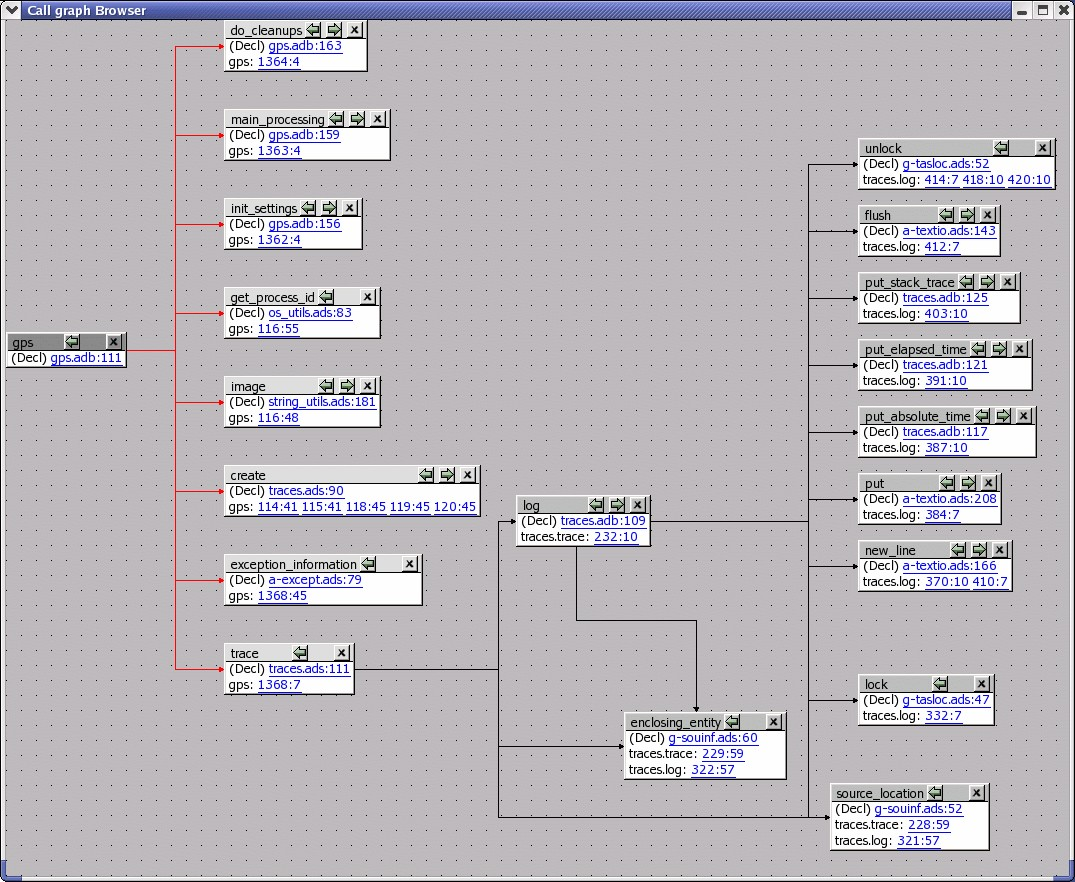
\includegraphics{call-graph.jpg}

In this browser, clicking on the right arrow in the title bar will display all
the entities that are called by the selected item.

Clicking on the left arrow will display all the entities that call the selected
item (i.e. its callers).

This browser is accessible through the contextual menu in the project view and
source editor, by selecting one of the items:

All boxes in this browser list several information: the location of their
declaration, and the list of all their references in the other entities
currently displayed in the browser. If you close the box for an entity that
calls them, the matching references are also hidden, to keep the contents of
the browser simpler.

\emph{Browsers-\textgreater{}*Entity} calls*
\begin{quote}

Display all the entities called by the selected entity. This has the same
effect as clicking on the right title bar arrow if the item is already
present in the call graph.
\end{quote}

\emph{Browsers-\textgreater{}*Entity} is called by*
\begin{quote}

Display all the entities called by the selected entity. This has the same
effect as clicking on the left title bar arrow if the item is already present
in the call graph.
\end{quote}

The contextual menu available by right-clicking on the entities in the browser
has the following new entries, in addition to the ones added by other modules
of GPS.
\begin{description}
\item[{\emph{Entity} calls}] \leavevmode
Same as described above.

\item[{\emph{Entity} is called by}] \leavevmode
Same as described above.

\item[{Go To Spec}] \leavevmode
Selecting this item will open a source editor that displays the
declaration of the entity.

\item[{Go To Body}] \leavevmode
Selecting this item will open a source editor that displays the
body of the entity.

\item[{Locate in Project View}] \leavevmode
Selecting this menu entry will move the focus to the project view,
and select the first node representing the file in which the entity is
declared. This makes it easier to see which other entities are
declared in the same file.

\end{description}


\section{Dependency Browser}
\label{browsing:id4}\label{browsing:dependency-browser}
\index{dependency browser}
The dependency browser shows the dependencies between source files. Each item
in the browser represents one source file.

\index{screen shot}
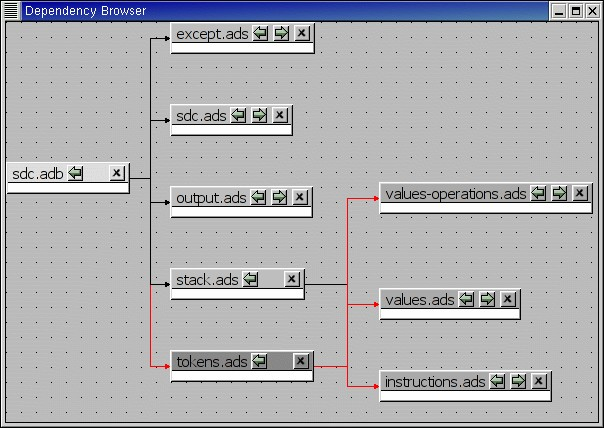
\includegraphics{dependency-browser.jpg}

In this browser, clicking on the right arrow in the title bar will display the
list of files that the selected file depends on. A file depend on another one
if it explicitly imports it (\emph{with} statement in Ada, or \emph{\#include} in C/C++).
Implicit dependencies are currently not displayed in this browser, since the
information is accessible by opening the other direct dependencies.

Clicking on the left arrow in the title bar will display the list of files that
depend on the selected file.

This browser is accessible through the contextual menu in the project view and
the source editor, by selecting one of the following items:
\begin{description}
\item[{\emph{Show dependencies for *file*}}] \leavevmode
\index{show dependencies for}
This has the same effect as clicking on the right arrow for a file already in
the browser, and will display the direct dependencies for that file.

\item[{\emph{Show files depending on *file*}}] \leavevmode
\index{show files depending on}
This has the same effect as clicking on the left arrow for a file already in
the browser, and will display the list of files that directly depend on that
file.

\end{description}

The background contextual menu in the browser adds a few entries to the
standard menu:

\emph{Open file...}
\begin{quote}

This menu entry will display an external dialog in which you can select the
name of a file to analyze.
\end{quote}

\emph{Recompute dependencies}
\begin{quote}

\index{recompute dependencies}
This menu entry will check that all links displays in the dependency browser
are still valid. If not, they are removed. The arrows in the title bar are
also reset if necessary, in case new dependencies were added for the files.

The browser is not refreshed automatically, since there are lots of cases
where the dependencies might change (editing source files, changing the
project hierarchy or the value of the scenario variables, ...)

It also recomputes the layout of the graph, and will change the current
position of the boxes.
\end{quote}
\begin{description}
\item[{\emph{Show system files}}] \leavevmode
\index{show system files}
This menu entry indicates whether standard system files (runtime files for
instance in the case of Ada) are displayed in the browser. By default, these
files will only be displayed if you explicitly select them through the \emph{Open
file} menu, or the contextual menu in the project view.

\item[{\emph{Show implicit dependencies}}] \leavevmode
\index{show implicit dependencies}
This menu entry indicates whether implicit dependencies should also be
displayed for the files. Implicit dependencies are files that are required to
compile the selected file, but that are not explicitly imported through a
\emph{with} or \emph{\#include} statement. For instance, the body of generics in Ada is
an implicit dependency.  Any time one of the implicit dependencies is
modified, the selected file should be recompiled as well.

\end{description}

The contextual menu available by right clicking on an item also adds a
number of entries:
\begin{description}
\item[{\emph{Analyze other file}}] \leavevmode
\index{analyze other file}
This will open a new item in the browser, displaying the complement file for
the selected one. In Ada, this would be the body if you clicked on a spec
file, or the opposite. In C, it depends on the naming conventions you
specified in the project properties, but you would generally go from a
\code{.h} file to a \code{.c} file and back.

\item[{\emph{Show dependencies for *file*}}] \leavevmode
\index{show files depending on file}
These play the same role as in the project view contextual menu

\end{description}


\section{Entity Browser}
\label{browsing:id5}\label{browsing:entity-browser}
\index{entity browser}
The entity browser displays static information about any source entity.

The exact content of the items depend on the type of the item. For instance:

\emph{Ada record / C struct}
\begin{quote}

The list of fields, each as an hyper link, is displayed. Clicking on
one of the fields will open a new item for the type.
\end{quote}

\emph{Ada tagged type / C++ class}
\begin{quote}

The list of attributes and methods is displayed. They are also
click-able hyper-links.
\end{quote}

\emph{Subprograms}
\begin{quote}

The list of parameters is displayed
\end{quote}

\emph{Packages}
\begin{quote}

The list of all the entities declared in that package is displayed
\end{quote}

\emph{and more...}

\index{screen shot}
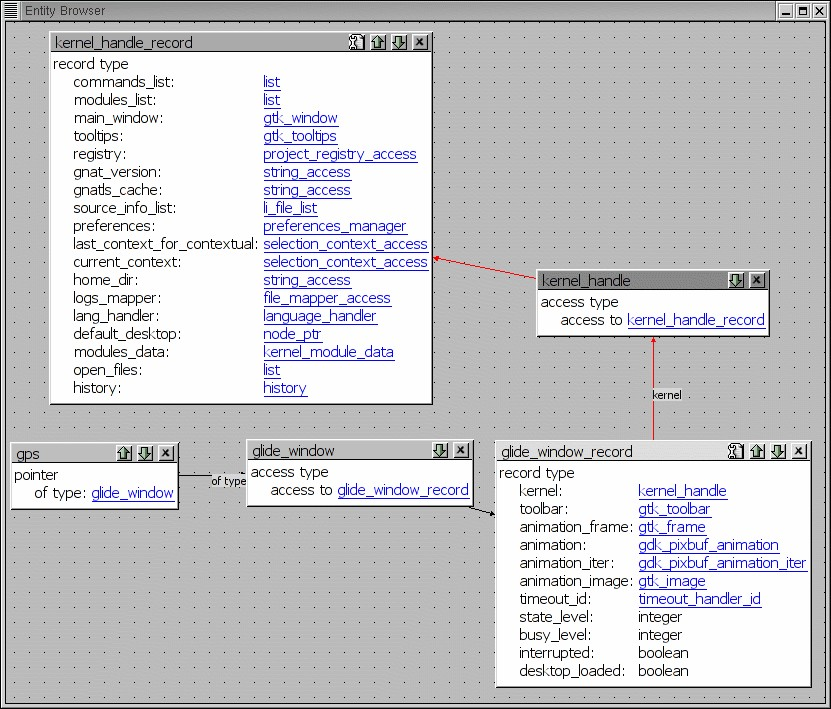
\includegraphics{entity-browser.jpg}

This browser is accessible through the contextual menu in the project view and
source editor, when clicking on an entity:
\begin{description}
\item[{\emph{Browsers/Examine entity *entity*}}] \leavevmode
\index{examine entity}
Open a new item in the entity browser that displays information for the
selected entity.

\end{description}

Most information in the items are click-able (by default, they appear as
underlined blue text). Clicking on one of these hyper links will open a new
item in the entity browser for the selected entity.

This browser can display the parent entities for an item. For instance, for a
C++ class or Ada tagged type, this would be the types it derives from. This is
accessible by clicking on the up arrow in the title bar of the item.

Likewise, children entities (for instance types that derive from the item) can
be displayed by clicking on the down arrow in the title bar.

An extra button appear in the title bar for the C++ class or Ada tagged types,
which toggles whether the inherited methods (or primitive operations in Ada)
should be displayed. By default, only the new methods, or the ones that
override an inherited one, are displayed. The parent's methods are not shown,
unless you click on this title bar button.


\chapter{Debugging}
\label{debugging:debugging}\label{debugging::doc}\label{debugging:id1}
\index{debugger}
\index{debugging}
GPS is also a graphical front-end for text-based debuggers such as GDB.  A
knowledge of the basics of the underlying debugger used by GPS will help
understanding how GPS works and what kind of functionalities it provides.

Please refer to the debugger-specific documentation - e.g. the GNAT User's
Guide (chapter \emph{Running and Debugging Ada Programs}) or the GDB documentation
for more details.

Debugging is tightly integrated with the other components of GPS. For example,
it is possible to edit files and navigate through your sources while debugging.

\index{menu}
To start a debug session, go to the menu \emph{Debug-\textgreater{}Initialize}, and choose either
the name of your executable, if you have specified the name of your main
program(s) in the project properties, or start an empty debug session using the
\emph{\textless{}no main file\textgreater{}} item. It is then possible to load any file to debug, by using
the menu \emph{Debug-\textgreater{}Debug-\textgreater{}Load File...}

Note that you first need to build your executable with debug information (\emph{-g}
switch), either explicitly as part of your project properties, or via the
\emph{Debug} build mode (see {\hyperref[compilation:the-build-mode]{\emph{The Build Mode}}} for more details).

Note that you can create multiple debuggers by using the \emph{Initialize} menu
several times: this will create a new debugger each time.  All the
debugger-related actions (e.g. stepping, running) are performed on the current
debugger, which is represented by the current debugger console.  To switch
between debuggers, simply select its corresponding console.

After the debugger has been initialized, you have access to two new windows:
the data window (in the top of the working area), and the debugger console (in
a new page, after the Messages and Shell windows).  All the menus under
\emph{Debugger} are now also accessible, and you also have access to additional
contextual menus, in particular in the source editor where it is possible to
easily display variables, set breakpoints, and get automatic display (via \emph{tool
tips}) of object values.

\index{menu}
When you want to quit the debugger without quitting GPS, go to the menu
\emph{Debug-\textgreater{}Terminate Current}, that will terminate your current debug session, or
the menu \emph{Debug-\textgreater{}Terminate} that will terminate all your debug sessions at
once.


\section{The Debug Menu}
\label{debugging:the-debug-menu}\label{debugging:id2}
\index{menu}
\index{debug}
\index{debugger}
The \emph{Debug} entry in the menu bar provides operations that act at a global
level. Key shortcuts are available for the most common operations, and are
displayed in the menus themselves.  Here is a detailed list of the menu items
that can be found in the menu bar:
\begin{description}
\item[{\emph{Run...}}] \leavevmode
\index{run}
Opens a dialog window allowing you to specify the arguments to pass to the
program to be debugged, and whether this program should be stopped at the
beginning of the main subprogram. If you confirm by clicking on the \emph{OK}
button, the program will be launched according to the arguments entered.

\item[{\emph{Step}}] \leavevmode
\index{step}
Execute the program until it reaches a different source line.

\item[{\emph{Step Instruction}}] \leavevmode
\index{stepi}
Execute the program for one machine instruction only.

\item[{\emph{Next}}] \leavevmode
\index{next}
Execute the program until it reaches the next source line, stepping over
subroutine calls.

\item[{\emph{Next Instruction}}] \leavevmode
\index{nexti}
Execute the program until it reaches the next machine instruction, stepping
over subroutine calls.

\item[{\emph{Finish}}] \leavevmode
\index{finish}
Continue execution until selected stack frame returns.

\item[{\emph{Continue}}] \leavevmode
\index{continue}
Continue execution of the program being debugged.

\item[{\emph{Interrupt}}] \leavevmode
\index{interrupt}
Asynchronously interrupt the program being debugged. Note that depending on
the state of the program, you may stop it in low-level system code that does
not have debug information, or in some cases, not even a coherent state. Use
of breakpoints is preferable to interrupting programs. Interrupting programs
is nevertheless required in some situations, for example when the program
appears to be in an infinite (or at least very time-consuming) loop.

\item[{\emph{Terminate Current}}] \leavevmode
\index{terminate}
Terminate the current debug session by terminating the underlying debugger
(e.g \emph{gdb}) used to handle the low level debugging. You can control what
happens to the windows through the \emph{Debugger/Debugger Windows} preference.

\item[{\emph{Terminate}}] \leavevmode
\index{terminate}
Terminate all your debug sessions. Same as \emph{Terminate Current} if there is
only one debugger open.

\end{description}


\subsection{Initialize}
\label{debugging:initialize}
This menu contains one entry per main unit defined in your project, which
will start a debug session and load the executable associated with the main
unit selected and if relevant, all corresponding settings: a debug session
will open the debug perspective and associated debug properties (e.g.
saved breakpoints, and data display).

\emph{\textless{}No Main File\textgreater{}}
\begin{quote}

Will initialize the debugger with no executable. You can then use one of
the menu items in the \emph{Debug} menu (e.g. \emph{Load File...} or \emph{Attach...})
if needed.
\end{quote}


\subsection{Debug}
\label{debugging:debug}\begin{description}
\item[{\emph{Connect to Board...}}] \leavevmode
\index{connect}
\index{board}
\index{target}
\index{cross debugger}
Opens a simple dialog to connect to a remote board. This option is only
relevant to cross debuggers.

\item[{\emph{Load File...}}] \leavevmode
\index{load}\phantomsection\label{debugging:open-program-menu}
Opens a file selection dialog that allows you to choose a program to debug.
The program to debug is either an executable for native debugging, or a
partially linked module for cross environments (e.g VxWorks).

\item[{\emph{Add Symbols...}}] \leavevmode
\index{add symbols}
Add the symbols from a given file/module. This corresponds to the gdb command
\emph{add-symbol-file}. This menu is particularly useful under VxWorks targets,
where the modules can be loaded independently of the debugger.  For instance,
if a module is independently loaded on the target (e.g. using windshell), it
is absolutely required to use this functionality, otherwise the debugger
won't work properly.

\item[{\emph{Attach...}}] \leavevmode
\index{attach}
Instead of starting a program to debug, you can instead attach to an already
running process. To do so, you need to specify the process id of the process
you want to debug. The process might be busy in an infinite loop, or waiting
for event processing. Note that as for {\hyperref[debugging:core-files]{\emph{Core Files}}}, you
need to specify an executable before attaching to a process.

\item[{\emph{Detach}}] \leavevmode
\index{detach}
Detaches the currently debugged process from the underlying debugger.  This
means that the executable will continue to run independently. You can use the
\emph{Attach To Process} menu later to re-attach to this process.

\item[{\emph{Debug Core File...}}] \leavevmode
\index{core file}\phantomsection\label{debugging:core-files}
This will open a file selection dialog that allows you to debug a core file
instead of debugging a running process. Note that you must first specify an
executable to debug before loading a core file.

\item[{\emph{Kill}}] \leavevmode
\index{kill}
Kills the process being debugged.

\end{description}


\subsection{Data}
\label{debugging:data}
\index{menu}
\index{data}
Note that most items in this menu need to access the underlying debugger when
the process is stopped, not when it is running. This means that you first need
to stop the process on a breakpoint or interrupt it, before using the following
commands. Failing to do so will result in blank windows.

\emph{Data Window}
\begin{quote}

Displays the Data window. If this window already exists, it is raised so that
it becomes visible
\end{quote}
\begin{description}
\item[{\emph{Call Stack}}] \leavevmode
\index{call stack}
Displays the Call Stack window.
See {\hyperref[debugging:the-call-stack-window]{\emph{The Call Stack Window}}} for more details.

\item[{\emph{Threads}}] \leavevmode
\index{thread}
Opens a new window containing the list of threads currently present in the
executable as reported by the underlying debugger. For each thread, it will
give information such as internal identifier, name and status.  This
information is language- and debugger-dependent. You should refer to the
underlying debugger's documentation for more details.  As indicated above,
the process being debugged needs to be stopped before using this command,
otherwise a blank list will be displayed.

When supported by the underlying debugger, clicking on a thread will change
the context (variables, call stack, source file) displayed, allowing you to
inspect the stack of the selected thread.

\item[{\emph{Tasks}}] \leavevmode
\index{task}
For GDB only, this will open a new window containing the list of Ada tasks
currently present in the executable. Similarly to the thread window, you can
switch to a selected task context by clicking on it, if supported by GDB. See
the GDB documentation for the list of items displayed for each task.

As for the thread window, the process being debugged needs to be stopped
before using this window.

\index{screen shot}
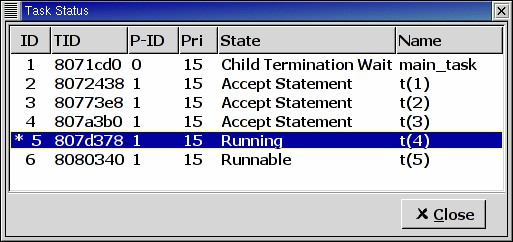
\includegraphics{tasks.jpg}

\item[{\emph{Protection Domains}}] \leavevmode
\index{protection domain}
For VxWorks AE only, this will open a new window containing the list of
available protection domains in the target. To change to a different
protection domain, simply click on it. A @c\{*\} character indicates the
current protection domain.

\item[{\emph{Assembly}}] \leavevmode
\index{assembly}
Opens a new window displaying an assembly dump of the current code being
executed.  See {\hyperref[debugging:the-assembly-window]{\emph{The Assembly Window}}} for more details.

\item[{\emph{Edit Breakpoints}}] \leavevmode
\index{breakpoint}
Opens an advanced window to create and modify any kind of breakpoint,
including watchpoints (see {\hyperref[debugging:the-breakpoint-editor]{\emph{The Breakpoint Editor}}}).  For simple
breakpoint creation, see the description of the source window.

\item[{\emph{Examine Memory}}] \leavevmode
\index{memory view}
Opens a memory viewer/editor. See {\hyperref[debugging:the-memory-window]{\emph{The Memory Window}}} for more details.

\item[{\emph{Command History}}] \leavevmode
\index{command}
\index{history}
Opens a dialog with the list of commands executed in the current session.
You can select any number of items in this list and replay the selection
automatically.

\item[{\emph{Display Local Variables}}] \leavevmode
\index{local variables}
Opens an item in the Data Window containing all the local variables for the
current frame.

\item[{\emph{Display Arguments}}] \leavevmode
\index{arguments}
Opens an item in the Data Window containing the arguments for the current
frame.

\item[{\emph{Display Registers}}] \leavevmode
\index{registers}
Opens an item in the Data Window containing the machine registers for the
current frame.

\item[{\emph{Display Any Expression...}}] \leavevmode
\index{display expression}
Opens a small dialog letting you specify an arbitrary expression in the Data
Window. This expression can be a variable name, or a more complex expression,
following the syntax of the underlying debugger.  See the documentation of
e.g gdb for more details on the syntax.  The check button \emph{Expression is a
subprogram call} should be enabled if the expression is actually a debugger
command (e.g \emph{p/x var}) or a procedure call in the program being debugged
(e.g \emph{call my\_proc}).

\item[{\emph{Recompute}}] \leavevmode
\index{recompute}
Recomputes and refreshes all the items displayed in the Data Window.

\end{description}


\section{The Call Stack Window}
\label{debugging:id3}\label{debugging:the-call-stack-window}
\index{call stack}
The call stack window gives a list of frames corresponding to the current
execution stack for the current thread/task.

\index{screen shot}
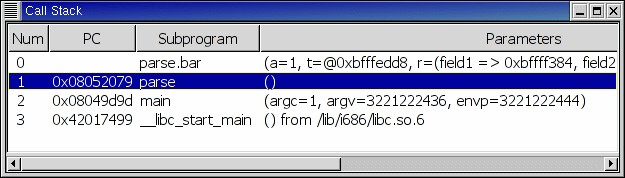
\includegraphics{call-stack.jpg}

The bottom frame corresponds to the outermost frame where the thread is
currently stopped. This frame corresponds to the first function executed by the
current thread (e.g main if the main thread is in C).  You can click on any
frame to switch to the caller's context, this will update the display in the
source window. See also the up and down buttons in the tool bar to go up and
down one frame in the call stack.

\index{contextual menu}
The contextual menu (right mouse button) allows you to choose which information
you want to display in the call stack window (via check buttons):
\begin{itemize}
\item {} 
Frame number: the debugger frame number (usually starts at 0 or 1)

\item {} 
Program Counter: the low level address corresponding to the
function's entry point.

\item {} 
Subprogram Name: the name of the subprogram in a given frame

\item {} 
Parameters: the parameters of the subprogram

\item {} 
File Location: the filename and line number information.

\end{itemize}

By default, only the subprogram name is displayed.  You can hide the call stack
window by closing it, as for other windows, and show it again using the menu
\emph{Data-\textgreater{}Call Stack}.


\section{The Data Window}
\label{debugging:the-data-window}\label{debugging:id4}
\index{data}
\index{data window}

\subsection{Description}
\label{debugging:index-48}\label{debugging:description}
The Data Window is the area in which various information about the debugged
process can be displayed. This includes the value of selected variables, the
current contents of the registeres, the local variables, ...

\index{Data Window}
This window is not open by default when you start the debugger. It will be
created automatically when needed (e.g. when using the Debug constextual menu
to display a variable). You can also force its display through the menu
\emph{Debug-\textgreater{}Data-\textgreater{}Data Window}.

However, if you save the desktop through the menu \emph{File-\textgreater{}Save More-\textgreater{}Desktop}
while the data window is open, it will be automatically reopen the next time
the desktop is loaded, for instance when restarting GPS.

The contents of the data window is preserved by default whenever you close it.
Thus, if you reopen the data window either during the same debugger session, or
automatically when you start a debugger on the same executable, it will display
the same items again. This behavior is controlled by the \emph{Preserve State on
Exit} preference.

\index{menu}
\index{contextual menu}
The data window contains all the graphic boxes that can be accessed using the
\emph{Data-\textgreater{}Display} menu items, or the data window \emph{Display Expression...}
contextual menu, or the source window \emph{Display} contextual menu items, or
finally the \emph{graph} command in the debugger console.

For each of these commands, a box is displayed in the data window with the
following information:

\index{screen shot}
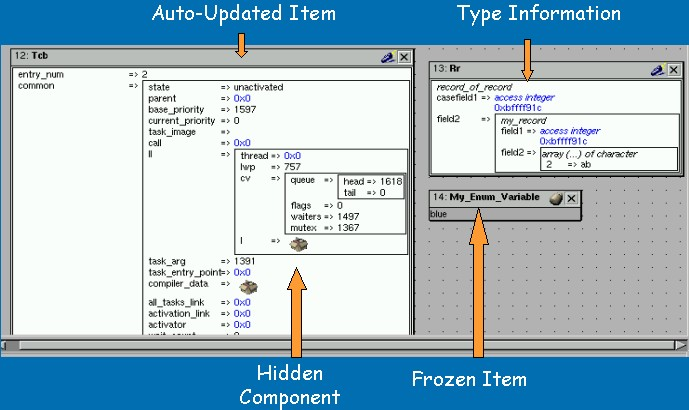
\includegraphics{canvas.jpg}
\begin{itemize}
\item {} 
A title bar containing:

\index{title bar}\begin{itemize}
\item {} 
The number of this expression: this is a positive number starting
from 1 and incremented for each new box displayed. It represents the
internal identifier of the box.

\item {} 
The name of the expression: this is the expression or variable
specified when creating the box.

\item {} 
An icon representing either a flash light, or a lock.
.. index:: icon

This is a click-able icon that will change the state of the box from
automatically updated (the flash light icon) to frozen (the lock icon).
When frozen, the value is grayed, and will not change until you change the
state. When updated, the value of the box will be recomputed each time an
execution command is sent to the debugger (e.g step, next).

\item {} 
An icon representing an `X'.
.. index:: icon

You can click on this icon to close/delete any box.

\end{itemize}

\item {} 
A main area.

The main area will display the data value hierarchically in a
language-sensitive manner. The canvas knows about data structures of various
languages (e.g \emph{C}, \emph{Ada}, \emph{C++}) and will organize them accordingly.  For
example, each field of a record/struct/class, or each item of an array will
be displayed separately. For each subcomponent, a thin box is displayed to
distinguish it from the other components.

\end{itemize}

\index{contextual menu}
A contextual menu, that takes into account the current component selected by
the mouse, gives access to the following capabilities:
\begin{description}
\item[{\emph{Close *component*}}] \leavevmode
Closes the selected item.

\item[{\emph{Hide all *component*}}] \leavevmode
\index{hide}
Hides all subcomponents of the selected item. To select a particular field or
item in a record/array, move your mouse over the name of this component, not
over the box containing the values for this item.

\item[{\emph{Show all *component*}}] \leavevmode
\index{show}
Shows all subcomponents of the selected item.

\item[{\emph{Clone *component*}}] \leavevmode
\index{clone}
Clones the selected component into a new, independent item.

\item[{\emph{View memory at address of *component*}}] \leavevmode
\index{memory view}
Brings up the memory view dialog and explore memory at the address of the
component.

\end{description}

\emph{Set value of *component*}
\begin{quote}

Sets the value of a selected component. This will open an entry box where you
can enter the new value of a variable/component. Note that GDB does not
perform any type or range checking on the value entered.
\end{quote}
\begin{description}
\item[{\emph{Update Value}}] \leavevmode
\index{update value}
Refreshes the value displayed in the selected item.

\item[{\emph{Show Value}}] \leavevmode
\index{show value}
Shows only the value of the item.

\item[{\emph{Show Type}}] \leavevmode
\index{show type}
Shows only the type of each field for the item.

\item[{\emph{Show Value+Type}}] \leavevmode
Shows both the value and the type of the item.

\item[{\emph{Auto refresh}}] \leavevmode
\index{auto refresh}
Enables or disables the automatic refreshing of the item upon program
execution (e.g step, next).

\end{description}

\index{contextual menu}
A contextual menu can be accessed in the canvas itself (point the mouse to an
empty area in the canvas, and click on the right mouse button) with the
following entries:
\begin{description}
\item[{\emph{Display Expression...}}] \leavevmode
\index{display expression}
Open a small dialog letting you specify an arbitrary expression in the Data
Window. This expression can be a variable name, or a more complex expression,
following the syntax of the current language and underlying debugger.  See
the documentation of e.g gdb for more details on the syntax.  The check
button \emph{Expression is a subprogram call} should be enabled if the expression
is actually not an expression but rather a debugger command (e.g \emph{p/x var})
or a procedure call in the program being debugged (e.g \emph{call my\_proc}).

\item[{\emph{Align On Grid}}] \leavevmode
\index{align}
Enables or disables alignment of items on the grid.

\item[{\emph{Detect Aliases}}] \leavevmode
\index{aliases}
Enables or disables the automatic detection of shared data structures.  Each
time you display an item or dereference a pointer, all the items already
displayed on the canvas are considered and their addresses are compared with
the address of the new item to display. If they match, (for example if you
tried to dereference a pointer to an object already displayed) instead of
creating a new item a link will be displayed.

\item[{\emph{Zoom in}}] \leavevmode
\index{zoom in}
Redisplays the items in the data window with a bigger font

\item[{\emph{Zoom out}}] \leavevmode
\index{zoom out}
Displays the items in the data window with smaller fonts and pixmaps. This
can be used when you have several items in the window and you can't see all
of them at the same time (for instance if you are displaying a tree and want
to clearly see its structure).

\item[{\emph{Zoom}}] \leavevmode
\index{zoom}
Allows you to choose the zoom level directly from a menu.

\item[{\emph{Clear}}] \leavevmode
\index{clear}
When this item is selected, all the boxes currently displayed are removed.

\end{description}


\subsection{Manipulating items}
\label{debugging:manipulating-items}

\subsubsection{Moving items}
\label{debugging:moving-items}
All the items on the canvas have some common behavior and can be fully
manipulated with the mouse.  They can be moved freely anywhere on the canvas,
simply by clicking on them and then dragging the mouse. Note that if you are
trying to move an item outside of the visible area of the data window, the
latter will be scrolled so as to make the new position visible.

Automatic scrolling is also provided if you move the mouse while dragging an
item near the borders of the data window. As long as the mouse remains close to
the border and the button is pressed on the item, the data window is scrolled
and the item is moved. This provides an easy way to move an item a long
distance from its initial position.


\subsubsection{Colors}
\label{debugging:colors}
Most of the items are displayed using several colors, each conveying a special
meaning. Here is the meaning assigned to all colors (note that the exact color
can be changed through the preferences dialog; these are the default colors):

\index{screen shot}
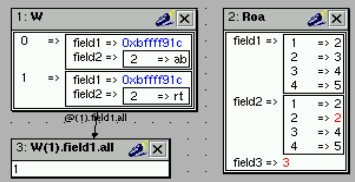
\includegraphics{colors.jpg}

\emph{black}
\begin{quote}

This is the default color used to print the value of variables or
expressions.
\end{quote}
\begin{description}
\item[{\emph{blue}}] \leavevmode
\index{C}
\index{Ada}
This color is used for C pointers (or Ada access values), i.e. all the
variables and fields that are memory addresses that denote some other value
in memory.

You can easily dereference these (that is to say see the value pointed to) by
double-clicking on the blue text itself.

\end{description}

\emph{red}
\begin{quote}

This color is used for variables and fields whose value has changed since the
data window was last displayed. For instance, if you display an array in the
data window and then select the \emph{Next} button in the tool bar, then the
elements of the array whose value has just changed will appear in red.

\index{menu}
As another example, if you choose to display the value of local variables in
the data window (\emph{Display-\textgreater{}Display Local Variables}), then only the variables
whose value has changed are highlighted, the others are left in black.
\end{quote}


\subsubsection{Icons}
\label{debugging:icons}
\index{icon}
Several different icons can be used in the display of items. They also convey
special meanings.

\emph{trash bin icon}
\begin{quote}

This icon indicates that the debugger could not get the value of the variable
or expression. There might be several reasons, for instance the variable is
currently not in scope (and thus does not exist), or it might have been
optimized away by the compiler. In all cases, the display will be updated as
soon as the variable becomes visible again.
\end{quote}

\emph{package icon}
\begin{quote}

This icon indicates that part of a complex structure is currently hidden.
Manipulating huge items in the data window (for instance if the variable is
an array of hundreds of complex elements) might not be very helpful. As a
result, you can shrink part of the value to save some screen space and make
it easier to visualize the interesting parts of these variables.

Double-clicking on this icon will expand the hidden part, and clicking on any
sub-rectangle in the display of the variable will hide that part and replace
it with that icon.

See also the description of the contextual menu to automatically show or hide
all the contents of an item. Note also that one alternative to hiding
subcomponents is to clone them in a separate item (see the contextual menu
again).
\end{quote}


\section{The Breakpoint Editor}
\label{debugging:id5}\label{debugging:the-breakpoint-editor}
\index{breakpoint editor}
\index{breakpoint}
\index{screen shot}
\index{menu}
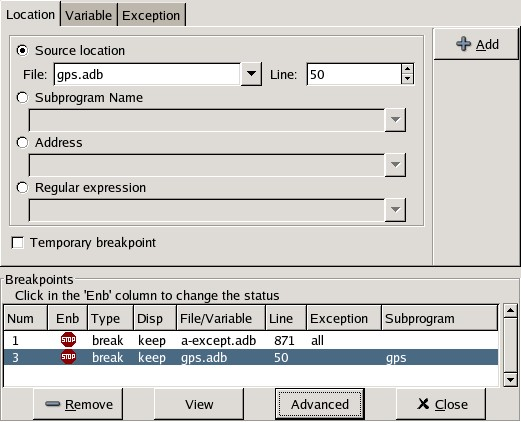
\includegraphics{breakpoints.jpg}

The breakpoint editor can be accessed from the menu \emph{Data-\textgreater{}Edit Breakpoints}.
It allows manipulation of different kinds of breakpoints: at a source location,
on a subprogram, at an executable address, on memory access (watchpoints), and
on Ada exceptions.

You can double-click on any breakpoint in the list to open the corresponding
source editor at the right location. Alternatively, you can select the
breakpoint and then click on the \emph{View} button.

The top area provides an interface to create the different kinds of
breakpoints, while the bottom area lists existing breakpoints and their
characteristics.

It is possible to access advanced breakpoint characteristics for a given
breakpoint.  First, select a breakpoint in the list.  Then, click on the
\emph{Advanced} button, which will display a new dialog window.  You can specify
commands to run automatically after a breakpoint is hit, or specify how many
times a selected breakpoint will be ignored.  If running VxWorks AE, you can
also change the Scope and Action settings for breakpoints.

\index{screen shot}
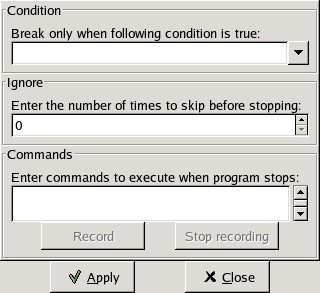
\includegraphics{bp-advanced.jpg}


\subsection{Scope/Action Settings for VxWorks AE}
\label{debugging:scope-action-settings-for-vxworks-ae}
\index{VxWorks AE}
In VxWorks AE breakpoints have two extra properties:
\begin{itemize}
\item {} 
Scope:
.. index:: scope

which task(s) can hit a given breakpoint. Possible Scope values are:
\begin{itemize}
\item {} 
task:
.. index:: task

the breakpoint can only be hit by the task that was active when the
breakpoint was set. If the breakpoint is set before the program is run, the
breakpoint will affect the environment task

\item {} 
pd:
.. index:: protection domain

any task in the current protection domain can hit that breakpoint

\item {} 
any:

any task in any protection domain can hit that breakpoint. This setting is
only allowed for tasks in the Kernel domain.

\end{itemize}

\item {} 
Action:
.. index:: action

when a task hits a breakpoints, which tasks are stopped:
\begin{itemize}
\item {} 
task:
.. index:: task

stop only the task that hit the breakpoint.

\item {} 
pd:
.. index:: protection domain

stop all tasks in the current protection domain

\item {} 
all:
stop all breakable tasks in the system

\end{itemize}

\end{itemize}

These two properties can be set/changed through the advanced breakpoints
characteristics by clicking on the \emph{Advanced} button. There are two ways of
setting these properties:
\begin{itemize}
\item {} 
Per breakpoint settings:

after setting a breakpoint (the default Scope/Action values will be
task/task), select the \emph{Scope/Action} tab in the \emph{Advanced} settings.  To
change these settings on a given breakpoint, select it from the breakpoints
list, select the desired values of Scope and Action and click on the \emph{Update}
button.

\item {} 
Default session settings:

select the \emph{Scope/Action} tab in the \emph{Advanced} settings. Select the desired
Scope and Action settings, check the \emph{Set as session defaults} check box
below and click the \emph{Close} button. From now on, every new breakpoint will
have the selected values for Scope and Action.

\end{itemize}

\index{saving breakpoints}
\index{breakpoints}\index{saving}
If you have enabled the preference \emph{Preserve state on exit}, GPS will
automatically save the currently set breakpoints, and restore them the next
time you debug the same executable. This allows you to immediately start
debugging your application again, without reseting the breakpoints every time.


\section{The Memory Window}
\label{debugging:id6}\label{debugging:the-memory-window}
\index{memory view}
\index{screen shot}
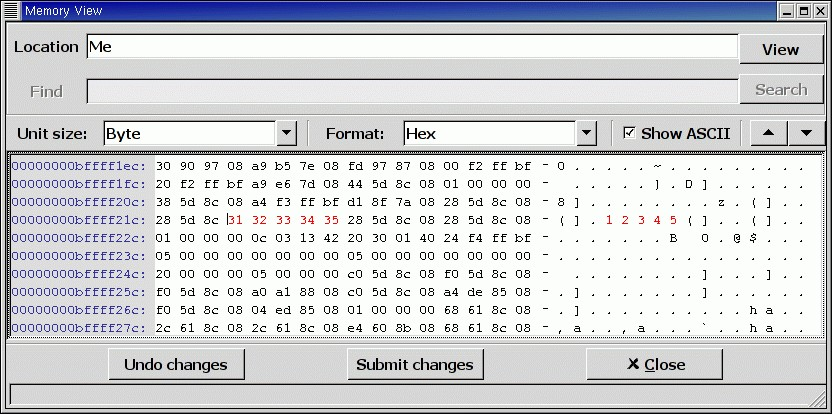
\includegraphics{memory-view.jpg}

The memory window allows you to display the contents of memory by
specifying either an address, or a variable name.

\index{C}
\index{hexadecimal}
To display memory contents, enter the address using the C hexadecimal notation:
0xabcd, or the name of a variable, e.g foo, in the \emph{Location} text entry.  In
the latter case, its address is computed automatically. Then either press
\emph{Enter} or click on the \emph{View} button. This will display the memory with the
corresponding addresses in the bottom text area.

\index{ASCII}
You can also specify the unit size (\emph{Byte}, \emph{Halfword} or \emph{Word}), the format
(\emph{Hexadecimal}, \emph{Decimal}, \emph{Octal} or \emph{ASCII}), and you can display the
corresponding ASCII value at the same time.

\index{key}
The \emph{up} and \emph{down} arrows as well as the \code{Page up} and \code{Page down}
keys in the memory text area allows you to walk through the memory in order of
ascending/descending addresses respectively.

Finally, you can modify a memory area by simply clicking on the location you
want to modify, and by entering the new values. Modified values will appear in
a different color (red by default) and will only be taken into account (i.e
written to the target) when you click on the \emph{Submit changes} button. Clicking
on the \emph{Undo changes} or going up/down in the memory will undo your editing.

Clicking on \emph{Close} will close the memory window, canceling your last pending
changes, if any.


\section{Using the Source Editor when Debugging}
\label{debugging:id7}\label{debugging:using-the-source-editor-when-debugging}
\index{source file}
\index{editing}
\index{debug}
When debugging, the left area of each source editor provides the following
information:

\emph{Lines with code}
\begin{quote}

In this area, blue dots are present next to lines for which the debugger has
debug information, in other words, lines that have been compiled with debug
information and for which the compiler has generated some code.  Currently,
there is no check when you try to set a breakpoint on a non dotted line: this
will simply send the breakpoint command to the underlying debugger, and
usually (e.g in the case of gdb) result in setting a breakpoint at the
closest location that matches the file and line that you specified.
\end{quote}
\begin{description}
\item[{\emph{Current line executed}}] \leavevmode
\index{current line}
This is a green arrow showing the line about to be executed.

\item[{\emph{Lines with breakpoints}}] \leavevmode
\index{breakpoint}
For lines where breakpoints have been set, a red mark is displayed on top of
the blue dot for the line. You can add and delete breakpoints by clicking on
this area (the first click will set a breakpoint, the second click will
remove it).

\end{description}

\index{screen shot}
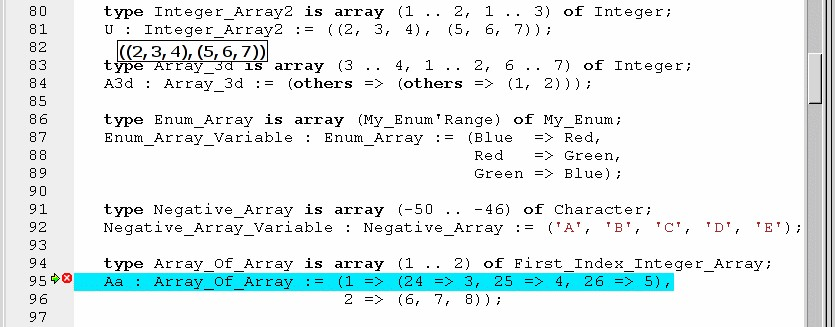
\includegraphics{tooltips.jpg}

\index{syntax highlighting}
\index{tooltip}
The second area in the source window is a text window on the right that
displays the source files, with syntax highlighting.  If you leave the cursor
over a variable, a tooltip will appear showing the value of this variable.
Automatic tooltips can be disabled in the preferences menu.

\index{preferences}
See {\hyperref[extending:preferences-dialog]{\emph{Preferences Dialog}}}.

\index{contextual menu}
When the debugger is active, the contextual menu of the source window contains
a sub menu called \emph{Debug} providing the following entries.

Note that these entries are dynamic: they will apply to the entity found under
the cursor when the menu is displayed (depending on the current language). In
addition, if a selection has been made in the source window the text of the
selection will be used instead. This allows you to display more complex
expressions easily (for example by adding some comments to your code with the
complex expressions you want to be able to display in the debugger).
\begin{description}
\item[{\emph{Print *selection*}}] \leavevmode
\index{print}
Prints the selection (or by default the name under the cursor) in the
debugger console.

\item[{\emph{Display *selection*}}] \leavevmode
\index{display}
Displays the selection (or by default the name under the cursor) in the data
window. The value will be automatically refreshed each time the process state
changes (e.g after a step or a next command). To freeze the display in the
canvas, you can either click on the corresponding icon in the data window, or
use the contextual menu for the specific item (see {\hyperref[debugging:the-data-window]{\emph{The Data Window}}} for
more information).

\item[{\emph{Print *selection}.all*}] \leavevmode
Dereferences the selection (or by default the name under the cursor) and
prints the value in the debugger console.

\item[{\emph{Display *selection}.all*}] \leavevmode
Dereferences the selection (or by default the name under the cursor) and
displays the value in the data window.

\item[{\emph{View memory at address of *selection*}}] \leavevmode
\index{memory view}
Brings up the memory view dialog and explores memory at the address of the
selection.

\item[{\emph{Set Breakpoint on Line *xx*}}] \leavevmode
\index{breakpoint}
Sets a breakpoint on the line under the cursor, in the current file.

\item[{\emph{Set Breakpoint on *selection*}}] \leavevmode
Sets a breakpoint at the beginning of the subprogram named \emph{selection}

\item[{\emph{Continue Until Line *xx*}}] \leavevmode
\index{continue until}
Continues execution (the program must have been started previously) until
it reaches the specified line.

\item[{\emph{Show Current Location}}] \leavevmode
\index{current location}
Jumps to the current line of execution. This is particularly useful after
navigating through your source code.

\end{description}


\section{The Assembly Window}
\label{debugging:the-assembly-window}\label{debugging:id8}
It is sometimes convenient to look at the assembly code for the subprogram
or source line you are currently debugging.

You can open the assembly window by using the menu
\emph{Debug-\textgreater{}Data-\textgreater{}Assembly}.

\index{screen shot}
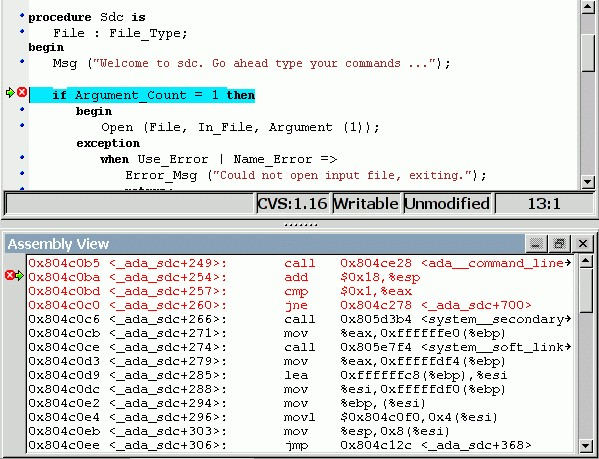
\includegraphics{assembly.jpg}

The current assembly instruction is highlighted with a green arrow on its left.
The instructions corresponding to the current source line are highlighted in
red by default. This allows you to easily see where the program counter will
point to, once you have pressed the ``Next'' button on the tool bar.

Moving to the next assembly instruction is done through the ``Nexti'' (next
instruction) button in the tool bar. If you choose ``Stepi'' instead (step
instruction), this will also jump to the subprogram being called.

For efficiency reasons, only a small part of the assembly code around the
current instruction is displayed.  You can specify in the {\hyperref[extending:preferences-dialog]{\emph{Preferences
Dialog}}} how many instructions are displayed by default.
Also, you can easily display the instructions immediately preceding or
following the currently displayed instructions by pressing one of the
\code{Page up} or \code{Page down} keys, or by using the contextual menu in the
assembly window.

A convenient complement when debugging at the assembly level is the ability of
displaying the contents  of machine registers.  When the debugger supports it
(as gdb does), you can select the \emph{Data-\textgreater{}Display Registers} menu to get an item
in the canvas that will show the current contents of each machine register, and
that will be updated every time one of them changes.

You might also choose to look at a single register.  With gdb, select the
\emph{Data-\textgreater{}Display Any Expression}, entering something like:

\begin{Verbatim}[commandchars=\\\{\}]
output /x \$eax
\end{Verbatim}

in the field, and selecting the toggle button ``Expression is a subprogram
call''. This will create a new canvas item that will be refreshed every time the
value of the register (in this case eax) changes.


\section{The Debugger Console}
\label{debugging:the-debugger-console}\label{debugging:id9}
\index{debugger}
\index{debugger console}
This is the text window located at the bottom of the main window.  In this
console, you have direct access to the underlying debugger, and can send
commands (you need to refer to the underlying debugger's documentation, but
usually typing \emph{help} will give you an overview of the commands available).

If the underlying debugger allows it, pressing \code{Tab} in this window will
provide completion for the command that is being typed (or for its arguments).

There are also additional commands defined to provide a simple text interface
to some graphical features.

Here is the complete list of such commands. The arguments between square
brackets are optional and can be omitted.

\emph{graph (print\textbar{}display) expression {[}dependent on display\_num{]} {[}link\_name name{]} {[}at x, y{]} {[}num num{]}}
\begin{quote}

\index{graph print}
\index{graph display}
This command creates a new item in the canvas, that shows the value of
\emph{Expression}. \emph{Expression} should be the name of a variable, or one of its
fields, that is in the current scope for the debugger.

The command \emph{graph print} will create a frozen item, that is not
automatically refreshed when the debugger stops, whereas \emph{graph display}
displays an automatically refreshed item.

The new item is associated with a number, that is visible in its title bar.
This number can be specified through the \emph{num} keyword, and will be taken
into account if no such item already exists.  These numbers can be used to
create links between the items, using the second argument to the command,
\emph{dependent on}. The link itself (i.e. the line) can be given a name that is
automatically displayed, using the third argument.
\end{quote}

\emph{graph (print\textbar{}display) {}`command{}`}
\begin{quote}

This command is similar to the one above, except it should be used to display
the result of a debugger command in the canvas.

For instance, if you want to display the value of a variable in hexadecimal
rather than the default decimal with gdb, you should use a command like:

\begin{Verbatim}[commandchars=\\\{\}]
graph display {}`print /x my\_variable{}`
\end{Verbatim}

This will evaluate the command between back-quotes every time the debugger
stops, and display this in the canvas. The lines that have changed will be
automatically highlighted (in red by default).

This command is the one used by default to display the value of registers for
instance.
\end{quote}

\emph{graph (enable\textbar{}disable) display display\_num {[}display\_num ...{]}}
\begin{quote}

\index{graph enable}
\index{graph disable}
This command will change the refresh status of items in the canvas. As
explained above, items are associated with a number visible in their title
bar.

Using the \emph{graph enable} command will force the item to be automatically
refreshed every time the debugger stops, whereas the \emph{graph disable} command
will freeze the item.
\end{quote}

\emph{graph undisplay display\_num}
\begin{quote}

\index{graph undisplay}
This command will remove an item from the canvas
\end{quote}


\section{Customizing the Debugger}
\label{debugging:id10}\label{debugging:customizing-the-debugger}
\index{debugger}
GPS is a high-level interface to several debugger backends, in particular gdb.
Each back end has its own strengths, but you can enhance the command line
interface to these backends through GPS, using Python.

This section will provide a small such example. The idea is to provide the
notion of ``alias'' in the debugger console. For example, this can be used so
that you type ``foo'', and this really executes a longer command, like displaying
the value of a variable with a long name.

\emph{gdb} already provides this feature through the \emph{define} keywords, but we will
in fact rewrite that feature in terms of python.

GPS provides an extensive Python API to interface with each of the running
debugger. In particular, it provides the function ``send'', which can be used to
send a command to the debugger, and get its output, and the function
``set\_output'', which can be used when you implement your own functions.

It also provides, through \emph{hook}, the capability to monitor the state of the
debugger back-end. In particular, one such hook, \emph{debugger\_command\_action\_hook}
is called when the user has typed a command in the debugger console, and before
the command is executed. This can be used to add your own commands. The example
below uses this hook.

Here is the code:

\begin{Verbatim}[commandchars=\\\{\}]
\PYG{k+kn}{import} \PYG{n+nn}{GPS}

\PYG{n}{aliases}\PYG{o}{=}\PYG{p}{\PYGZob{}}\PYG{p}{\PYGZcb{}}

\PYG{k}{def} \PYG{n+nf}{set\PYGZus{}alias} \PYG{p}{(}\PYG{n}{name}\PYG{p}{,} \PYG{n}{command}\PYG{p}{)}\PYG{p}{:}
   \PYG{l+s+sd}{"""Set a new debugger alias. Typing this alias in a debugger window}
\PYG{l+s+sd}{      will then execute command"""}
   \PYG{k}{global} \PYG{n}{aliases}
   \PYG{n}{aliases}\PYG{p}{[}\PYG{n}{name}\PYG{p}{]} \PYG{o}{=} \PYG{n}{command}

\PYG{k}{def} \PYG{n+nf}{execute\PYGZus{}alias} \PYG{p}{(}\PYG{n}{debugger}\PYG{p}{,} \PYG{n}{name}\PYG{p}{)}\PYG{p}{:}
   \PYG{k}{return} \PYG{n}{debugger}\PYG{o}{.}\PYG{n}{send} \PYG{p}{(}\PYG{n}{aliases}\PYG{p}{[}\PYG{n}{name}\PYG{p}{]}\PYG{p}{,} \PYG{n}{output}\PYG{o}{=}\PYG{n+nb+bp}{False}\PYG{p}{)}

\PYG{k}{def} \PYG{n+nf}{debugger\PYGZus{}commands} \PYG{p}{(}\PYG{n}{hook}\PYG{p}{,} \PYG{n}{debugger}\PYG{p}{,} \PYG{n}{command}\PYG{p}{)}\PYG{p}{:}
   \PYG{k}{global} \PYG{n}{aliases}
   \PYG{n}{words} \PYG{o}{=} \PYG{n}{command}\PYG{o}{.}\PYG{n}{split}\PYG{p}{(}\PYG{p}{)}
   \PYG{k}{if} \PYG{n}{words}\PYG{p}{[}\PYG{l+m+mi}{0}\PYG{p}{]} \PYG{o}{==} \PYG{l+s}{"}\PYG{l+s}{alias}\PYG{l+s}{"}\PYG{p}{:}
      \PYG{n}{set\PYGZus{}alias} \PYG{p}{(}\PYG{n}{words}\PYG{p}{[}\PYG{l+m+mi}{1}\PYG{p}{]}\PYG{p}{,} \PYG{l+s}{"}\PYG{l+s}{ }\PYG{l+s}{"}\PYG{o}{.}\PYG{n}{join} \PYG{p}{(}\PYG{n}{words} \PYG{p}{[}\PYG{l+m+mi}{2}\PYG{p}{:}\PYG{p}{]}\PYG{p}{)}\PYG{p}{)}
      \PYG{k}{return} \PYG{n+nb+bp}{True}
   \PYG{k}{elif} \PYG{n}{aliases}\PYG{o}{.}\PYG{n}{has\PYGZus{}key} \PYG{p}{(}\PYG{n}{words} \PYG{p}{[}\PYG{l+m+mi}{0}\PYG{p}{]}\PYG{p}{)}\PYG{p}{:}
      \PYG{n}{debugger}\PYG{o}{.}\PYG{n}{set\PYGZus{}output} \PYG{p}{(}\PYG{n}{execute\PYGZus{}alias} \PYG{p}{(}\PYG{n}{debugger}\PYG{p}{,} \PYG{n}{words}\PYG{p}{[}\PYG{l+m+mi}{0}\PYG{p}{]}\PYG{p}{)}\PYG{p}{)}
      \PYG{k}{return} \PYG{n+nb+bp}{True}
   \PYG{k}{else}\PYG{p}{:}
      \PYG{k}{return} \PYG{n+nb+bp}{False}

\PYG{n}{GPS}\PYG{o}{.}\PYG{n}{Hook} \PYG{p}{(}\PYG{l+s}{"}\PYG{l+s}{debugger\PYGZus{}command\PYGZus{}action\PYGZus{}hook}\PYG{l+s}{"}\PYG{p}{)}\PYG{o}{.}\PYG{n}{add} \PYG{p}{(}\PYG{n}{debugger\PYGZus{}commands}\PYG{p}{)}
\end{Verbatim}

The list of aliases is stored in the global variable \emph{aliases}, which is
modified by \emph{set\_alias}. Whenever the user executes an alias, the real command
send to the debugger is sent through \emph{execute\_alias}.

The real part of the work is done by \emph{debugger\_commands}. If the user is
executing the \emph{alias} command, it defines a new alias. Otherwise, if he typed
the name of an alias, we really want to execute that alias. Else, we let the
debugger back-end handle that command.

After you have copied this example in the \code{\$HOME/.gps/plug-ins}
directory, you can start a debugger as usual in GPS, and type the following in
its console:

\begin{Verbatim}[commandchars=\\\{\}]
(gdb) alias foo print a\_long\_long\_name
(gdb) foo
\end{Verbatim}

The first command defines the alias, the second line executes it.

This alias can also be used within the \emph{graph display} command, so that the
value of the variable is in fact displayed in the data window automatically,
for instance:

\begin{Verbatim}[commandchars=\\\{\}]
(gdb) graph display {}`foo{}`
\end{Verbatim}

Other examples can be programmed. You could write complex python functions,
which would for instance query the value of several variables, and pretty print
the result. This complex python function can then be called from the debugger
console, or automatically every time the debugger stops through the \emph{graph
display} command.


\chapter{Version Control System}
\label{vcs:version-control-system}\label{vcs::doc}\label{vcs:id1}
\index{version control}
GPS offers the possibility for multiple developers to work on the same project,
through the integration of version control systems (VCS). Each project can be
associated to a VCS, through the \emph{VCS} tab in the Project properties editor.
{\hyperref[projects:the-project-properties-editor]{\emph{The Project Properties Editor}}}.

GPS does not come with any version control system: it uses underlying
command-line systems such as Subversion or ClearCase to perform the low level
operations, and provides a high level user interface on top of them. Be sure to
have a properly installed version control system before enabling it under GPS.

The systems that are supported out of the box in GPS are:
\begin{description}
\item[{\emph{Auto}}] \leavevmode
\index{VCS}\index{auto}
GPS can be setup to auto-detect the actual VCS to use for each project. This
is done by selecting \emph{Auto} in the \emph{VCS} tab of the Project properties
editor. {\hyperref[projects:the-project-properties-editor]{\emph{The Project Properties Editor}}}.  This is also the default
behavior when no VCS is specified in the project.

\item[{\emph{ClearCase}}] \leavevmode
\index{VCS}\index{ClearCase}
The standard ClearCase interface, which is built-in and uses a generic GPS
terminology for VCS operations.

Note that, at the moment, only Snapshot Views are supported in the ClearCase
integration; Dynamic Views are not supported.

\item[{\emph{ClearCase Native}}] \leavevmode
\index{VCS}\index{ClearCase Native}
Which is fully customizable and uses by default the terminology specific to
ClearCase.

Note that, at the moment, only Snapshot Views are supported in the ClearCase
integration; Dynamic Views are not supported.

\item[{\emph{CVS}}] \leavevmode
\index{VCS}\index{CVS}
The Concurrent Version System.

GPS needs a corresponding \emph{patch} command that usually comes with it.

\item[{\emph{Git}}] \leavevmode
\index{VCS}\index{Git}
Distributed fast source code management. Support for Git on GPS is partial.
Basic commands are supported but the full power of Git (like working with the
index) is only available on the command line.

GPS needs a corresponding \emph{diff} command that usually comes with it.

\item[{\emph{Mercurial}}] \leavevmode
\index{VCS}\index{Mercurial}
An experimental plugin for supporting Mercurial.

\item[{\emph{Subversion}}] \leavevmode
\index{VCS}\index{Subversion}
The Subversion version control system. Note that on Windows this version is
intended to be used with Cygwin/Subversion and fully supports the Cygwin path
names.

GPS needs a corresponding \emph{patch} and \emph{diff} command that usually comes with
it.

\item[{\emph{Subversion Windows}}] \leavevmode
\index{VCS}\index{Subversion Windows}
The Windows native Subversion version control system. The external Subversion
commands are expected to be built for the Win32 subsystem. This version does
not support Cygwin path names.

GPS needs a corresponding \emph{patch} and \emph{diff} command
that usually comes with it.

\end{description}

The default VCS that GPS will use is ``Auto'' by default, and this can be
configured through {\hyperref[extending:the-preferences-dialog]{\emph{The Preferences Dialog}}}.

It is also possible to add your own support for other version control systems,
or modify one of the existing interfaces, see
{\hyperref[extending:adding-support-for-new-version-control-systems]{\emph{Adding support for new Version Control Systems}}} for more information.

It is recommended that you first get familiar with the version control system
that you intend to use in GPS first, since many concepts used in GPS assume
basic knowledge of the underlying system.

Associating a VCS to a project enables the use of basic VCS features on the
source files contained in the project. Those basic features typically include
the checking in and out of files, the querying of file status, file revision
history, comparison between various revisions, and so on.

\index{password}
Note: the set-up must make sure that the VCS commands can be launched without
entering a password.


\section{The VCS Explorer}
\label{vcs:id2}\label{vcs:the-vcs-explorer}
\index{VCS explorer}
\index{version control}
The VCS Explorer provides an overview of source files and their status. A file
edited in GPS will be automatically added on the VCS Explorer with a Modified
status (see below).

\index{screen shot}
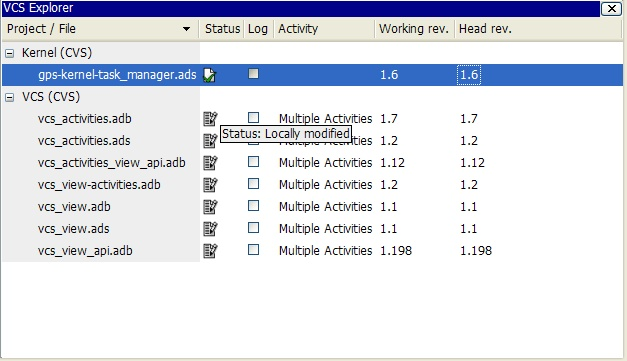
\includegraphics{vcs-explorer.jpg}

The easiest way to bring up the VCS Explorer is through the menu
\emph{VCS-\textgreater{}Explorer}. The Explorer can also be brought up using the contextual menu
\emph{Version Control-\textgreater{}Query status} on files, directories and projects in the file
and project views, and on file editors.
{\hyperref[vcs:the-version-control-contextual-menu]{\emph{The Version Control Contextual Menu}}}.

The VCS Explorer contains the following columns:
\begin{description}
\item[{\emph{Project / File}}] \leavevmode
This is a two levels tree, the first level contains the name of the project
and the second the name of files inside the project. Next to the project name
the VCS name, if any, is displayed. This is the only information available
for a project. The columns described below are for the files only. This
column can be sorted by clicking on the header.

\item[{\emph{Status}}] \leavevmode
Shows the status of the file. This column can be sorted by clicking on
the header. The different possible status for files are the following:
\begin{description}
\item[{\emph{Unknown}}] \leavevmode
\includegraphics{gps-vcs-unknown.jpg}

The status is not yet determined or the VCS repository is not able to
give this information (for example if it is unavailable, or locked).

\item[{\emph{Not registered}}] \leavevmode
\includegraphics{gps-vcs-not-registered.jpg}

The file is not known to the VCS repository.

\item[{\emph{Up-to-date}}] \leavevmode
\includegraphics{gps-vcs-up-to-date.jpg}

The file corresponds to the latest version in the corresponding branch
on the repository.

\item[{\emph{Added}}] \leavevmode
\includegraphics{gps-vcs-added.jpg}

The file has been added remotely but is not yet updated in the local
view.

\item[{\emph{Removed}}] \leavevmode
\includegraphics{gps-vcs-removed.jpg}

The file still exists locally but is known to have been removed from
the VCS repository.

\item[{\emph{Modified}}] \leavevmode
\includegraphics{gps-vcs-modified.jpg}

The file has been modified by the user or has been explicitly opened
for editing.

\item[{\emph{Needs merge}}] \leavevmode
\includegraphics{gps-vcs-needs-merge.jpg}

The file has been modified locally and on the repository.

\item[{\emph{Needs update}}] \leavevmode
\includegraphics{gps-vcs-needs-update.jpg}

The file has been modified in the repository but not locally.

\item[{\emph{Contains merge conflicts}}] \leavevmode
\includegraphics{gps-vcs-has-conflicts.jpg}

The file contains conflicts from a previous update operation.

\end{description}

\item[{\emph{Log}}] \leavevmode
This column indicates whether a revision log exists for this file.

\item[{\emph{Activity}}] \leavevmode
The name of the activity the file belongs to. See {\hyperref[vcs:the-vcs-activities]{\emph{The VCS Activities}}}
for more details.

\item[{\emph{Working rev.}}] \leavevmode
Indicates the version of the local file.

\item[{\emph{Head rev.}}] \leavevmode
Indicates the most recent version of the file in the repository.

\end{description}

The VCS Explorer supports multiple selections. To select a single line, simply
left-click on it. To select a range of lines, select the first line in the
range, then hold down the \code{Shift} key and select the last line in the
range. To add or remove single columns from the selection, hold down the
\code{Control} key and left-click on the columns that you want to
select/unselect. It is also possible to select files having the same status
using the \emph{Select files same status} menu entry. See
{\hyperref[vcs:the-version-control-contextual-menu]{\emph{The Version Control Contextual Menu}}}.

\index{interactive search}
The explorer also provides an {\hyperref[main_window:interactive-search]{\emph{interactive search}}}
capability allowing you to quickly look for a given file name. The default key
to start an interactive search is \code{Ctrl-i}.

The VCS contextual menu can be brought up from the VCS explorer by
left-clicking on a selection or on a single line.
{\hyperref[vcs:the-version-control-contextual-menu]{\emph{The Version Control Contextual Menu}}}.


\section{The VCS Activities}
\label{vcs:the-vcs-activities}\label{vcs:id3}
\index{VCS activities}
\index{version control}
The VCS Activities give the ability to group files to be committed together.
The set of files can be committed atomically if supported by the version
control system used.

\index{screen shot}
\includegraphics{vcs-activities.jpg}

The way to bring up the VCS Activities view is through the \emph{VCS-\textgreater{}Activities}
menu.

The VCS Activities view contains the following columns:
\begin{description}
\item[{\emph{Activity / File}}] \leavevmode
The name of the activity or files belonging to an activity. This
column can be sorted by clicking on the header.

\item[{\emph{Status}}] \leavevmode
Shows the status of the file. This column can be sorted by clicking on
the header. See {\hyperref[vcs:the-vcs-explorer]{\emph{The VCS Explorer}}} for a full description.

\item[{\emph{Log}}] \leavevmode
This column indicates whether a revision log exists for this file.

\item[{\emph{Working rev.}}] \leavevmode
Indicates the version of the local file.

\item[{\emph{Head rev.}}] \leavevmode
Indicates the most recent version of the file in the repository.

\end{description}

The VCS Explorer supports multiple selections. To select a single line, simply
left-click on it. To select a range of lines, select the first line in the
range, then hold down the \code{Shift} key and select the last line in the
range. To add or remove single columns from the selection, hold down the
\code{Control} key and left-click on the columns that you want to
select/unselect.

There are different contextual menu entries depending on the position on the
screen.  On an empty area we have a simple contextual menu:
\begin{description}
\item[{\emph{Create new activity}}] \leavevmode
Create a new activity. The name can be edited by double clicking on it.

\end{description}

On an activity line the contextual menu is:
\begin{description}
\item[{\emph{Group commit}}] \leavevmode
This is a selectable menu entry. It is activated only if the
VCS supports atomic commit and absolute filenames. See {\hyperref[extending:the-vcs-node]{\emph{The VCS node}}}
for full details.

\item[{\emph{Create new activity}}] \leavevmode
Create a new activity. The name can be edited by double clicking on it.

\item[{\emph{Re-open activity / Close activity}}] \leavevmode
If the activity is closed it is possible to re-open it and if it is
opened it is possible to close it manually.

\item[{\emph{Delete activity}}] \leavevmode
Remove the activity.

\item[{\emph{Commit activity}}] \leavevmode
Commit the activity. If group commit is activated then the commit log content
is generated using a template file fully configurable.  See {\hyperref[environment:files]{\emph{Files}}}.  If
group commit is not activated then the log content for each activity file is
the file log catenated with the activity log. After this operation the file's
log are removed but the activity log is kept as documentation.

\item[{\emph{Query status}}] \leavevmode
Query the status for all the source files contained in the activity.

\item[{\emph{Update}}] \leavevmode
Update all the source files contained in the activity.

\item[{\emph{Compare against head revision}}] \leavevmode
Show a visual comparison between the local activity files and the most recent
version of those files in the repository.

\item[{\emph{Build patch file}}] \leavevmode
Create a patch file (in text format) for the activity. The patch file
contains a header (the activity log and file's logs) and the diff of
each file. The header format is fully configurable using a template
file. See {\hyperref[environment:files]{\emph{Files}}}.

\item[{\emph{Edit revision log}}] \leavevmode
Edit the current revision log for activity. This log is shared with
all the activity files.

\item[{\emph{Remove revision log}}] \leavevmode
Remove the current revision log for activity. This menu is present
only if the activity revision log exists.

\end{description}

On a file line the contextual menu contains:
\begin{description}
\item[{\emph{Create new activity}}] \leavevmode
Create a new activity. The name can be edited by double clicking on it.

\item[{\emph{Remove from activity}}] \leavevmode
Remove the selected file from the activity and delete the activity log.

\item[{\emph{Edit revision log}}] \leavevmode
Edit the current revision log for the selected file.

\end{description}


\section{The VCS Menu}
\label{vcs:the-vcs-menu}\label{vcs:id4}
\index{version control}
\index{menu}
Basic VCS operations can be accessed through the VCS menu. Most of these
functions act on the current selection, i.e. on the selected items in the VCS
Explorer if it is present, or on the currently selected file editor, or on the
currently selected item in the \emph{Tools-\textgreater{}Views-\textgreater{}Files}.  In most cases, the VCS
contextual menu offers more control on VCS operations.
{\hyperref[vcs:the-version-control-contextual-menu]{\emph{The Version Control Contextual Menu}}}.
\begin{description}
\item[{\emph{Explorer}}] \leavevmode
Open or raise the VCS Explorer. {\hyperref[vcs:the-vcs-explorer]{\emph{The VCS Explorer}}}.

\item[{\emph{Update all projects}}] \leavevmode
Update the source files in the current project, and all imported
sub-projects, recursively.

\item[{\emph{Query status for all projects}}] \leavevmode
Query the status of all files in the project and all imported sub-projects.

\item[{\emph{Create tag...}}] \leavevmode
Create a tag or branch tag starting from a specific root
directory. The name of the tag is a simple name.

\item[{\emph{Switch tag...}}] \leavevmode
Switch the local copy to a specific tag. The name of the tag depends
on the external VCS used. For CVS this this the simple tag name, for
Subversion the tag must conform to the default repository layout. For
a branch tag this is \emph{/branches/\textless{}tag\_name\textgreater{}/\textless{}root\_dir\textgreater{}}.

\end{description}

For a description of the other entries in the VCS menu, see
{\hyperref[vcs:the-version-control-contextual-menu]{\emph{The Version Control Contextual Menu}}}


\section{The Version Control Contextual Menu}
\label{vcs:the-version-control-contextual-menu}\label{vcs:id5}
This section describes the version control contextual menu displayed when you
right-click on an entity (e.g. a file, a directory, a project) from various
parts of GPS, including the project view, the source editor and the VCS
Explorer.

Depending on the context, some of the items described in this section won't be
shown, which means that they are not relevant to the current context.
\begin{description}
\item[{\emph{Remove project}}] \leavevmode
Only displayed on a project line. This will remove the selected
project from the VCS Explorer.

\item[{\emph{Expand all}}] \leavevmode
Expand all VCS Explorer project nodes.

\item[{\emph{Collapse all}}] \leavevmode
Collapse all VCS Explorer project nodes.

\item[{\emph{Clear View}}] \leavevmode
Clear the VCS Explorer.

\item[{\emph{Query status}}] \leavevmode
Query the status of the selected item. Brings up the VCS Explorer.

\item[{\emph{Update}}] \leavevmode\phantomsection\label{vcs:update}
Update the currently selected item (file, directory or project).

\item[{\emph{Commit}}] \leavevmode\phantomsection\label{vcs:commit}
Submits the changes made to the file to the repository, and queries
the status for the file once the change is made.

It is possible to tell GPS to check the file before the actual commit
happens. This is done by specifying a \emph{File checker} in the \emph{VCS} tab of the
project properties dialog. This \emph{File checker} is in fact a script or
executable that takes an absolute file name as argument, and displays any
error message on the standard output. The VCS commit operation will actually
occur only if nothing was written on the standard output.

It is also possible to check the change-log of a file before commit, by
specifying a \emph{Log checker} in the project properties dialog. This works on
change-log files in the same way as the \emph{File checker} works on source files.

\item[{\emph{Open}}] \leavevmode\phantomsection\label{vcs:open}
Open the currently selected file for writing. On some VCS systems,
this is a necessary operation, and on other systems it is not.

\item[{\emph{View entire revision history}}] \leavevmode\phantomsection\label{vcs:view-revision-history}
Show the revision logs for all previous revisions of this file.

\item[{\emph{View specific revision history}}] \leavevmode
Show the revision logs for one previous revision of this file.

\item[{\emph{Compare against head revision}}] \leavevmode
\index{compare}\phantomsection\label{vcs:compare-against-head}
Show a visual comparison between the local file and the most recent
version of that file in the repository.

\item[{\emph{Compare against other revision}}] \leavevmode\phantomsection\label{vcs:compare-against-working}
Show a visual comparison between the local file and one specific
version of that file in the repository.

\item[{\emph{Compare two revisions}}] \leavevmode\phantomsection\label{vcs:compare-against-revision}
Show a visual comparison between two specific revisions
of the file in the repository.

\item[{\emph{Compare base against head}}] \leavevmode\phantomsection\label{vcs:compare-base-against-head}
Show a visual comparison between the corresponding version of the
file in the repository and the most recent version of that file.

\item[{\emph{Compare against tag/branch}}] \leavevmode\phantomsection\label{vcs:compare-base-against-tag-branch}
Only available on a Revision View and over a tag/branch. Show a visual
comparison between the corresponding version of the file in the repository
and the version of that file in the tag/branch.

\item[{\emph{Annotate}}] \leavevmode\phantomsection\label{vcs:annotate}
Display the annotations for the file, i.e. the information for each line of
the file showing the revision corresponding to that file, and additional
information depending on the VCS system.

When using CVS or Subversion, the annotations are clickable. Left-clicking on
an annotation line will query and display the changelog associated to the
specific revision for this line.

\item[{\emph{Remove Annotate}}] \leavevmode
Remove the annotations from the selected file.

\item[{\emph{Edit revision log}}] \leavevmode
Edit the current revision log for the selected file.

\item[{\emph{Edit global ChangeLog}}] \leavevmode
Edit the global ChangeLog entry for the selected file.
{\hyperref[vcs:working-with-global-changelog-file]{\emph{Working with global ChangeLog file}}}.

\item[{\emph{Remove revision log}}] \leavevmode
Clear the current revision associated to the selected file.

\item[{\emph{Add}}] \leavevmode
Add a file to the repository, using the current revision log for this
file. If no revision log exists, activating this menu will create
one. The file is committed in the repository.

\item[{\emph{Add/No commit}}] \leavevmode
Add a file to the repository, using the current revision log for this
file. If no revision log exists, activating this menu will create
one. The file is not committed in the repository.

\item[{\emph{Remove}}] \leavevmode
Remove a file from the repository, using the current revision log for
this file. If no revision log exists, activating this menu will create
one. The modification is committed in the repository.

\item[{\emph{Remove/No commit}}] \leavevmode
Remove a file from the repository, using the current revision log for
this file. If no revision log exists, activating this menu will create
one. The modification is not committed in the repository.

\item[{\emph{Revert}}] \leavevmode
Revert a locale file to the repository revision, discarding all local
changes.

\item[{\emph{Resolved}}] \leavevmode
Mark files' merge conflics as resolved. Some version control systems
(like Subversion) will block any commit until this action is called.

\item[{\emph{Switch tag/bracnh}}] \leavevmode
Only available on a Revision View and over a tag/branch name. Will
switch the tree starting from a selected root to this specific tag or
branch.

\item[{\emph{Merge}}] \leavevmode
Only available on a Revision View and over a tag/branch name. Merge
file changes made on this specific tag/branch.

\item[{\emph{View revision}}] \leavevmode
Only available on a Revision View and over a revision.

\item[{\emph{Commit as new Activity}}] \leavevmode
An action to prepare a group-commit in just one-click. This action will:

\end{description}

\emph{create an anonymous activity,}
\begin{quote}
\begin{description}
\item[{\emph{add all files selected into the VCS Explorer into the newly}}] \leavevmode
created anonymous activity,

\end{description}
\end{quote}
\begin{description}
\item[{\emph{open the activity log,}}] \leavevmode
Just fill the activity log and commit the anonymous activity.

\item[{\emph{Add to Activity}}] \leavevmode
A menu containing all the current activities. Selecting one will add
the current file to this activity. This menu is present only if the
file is not already part of an activity.

\item[{\emph{Remove from Activity}}] \leavevmode
Remove file from the given activity. This menu is present only if the
file is already part of an activity.

\item[{\emph{Directory}}] \leavevmode
Only available when the current context contains directory information
\begin{description}
\item[{\emph{Add/No commit}}] \leavevmode
Add the selected directory into the VCS.

\item[{\emph{Remove/No commit}}] \leavevmode
Remove the selected directory from the VCS.

\item[{\emph{Commit}}] \leavevmode
Commit the selected directory into the VCS. This action is available
only if the VCS supports commit on directories, {\hyperref[extending:the-vcs-node]{\emph{The VCS node}}}.

\item[{\emph{Add to Activity}}] \leavevmode
Add the selected directory into the VCS. This action is available
only if the VCS supports commit on directories, {\hyperref[extending:the-vcs-node]{\emph{The VCS node}}}.

\item[{\emph{Query status for directory}}] \leavevmode
Query status for the files contained in the selected directory.

\item[{\emph{Update directory}}] \leavevmode
Update the files in the selected directory.

\item[{\emph{Query status for directory recursively}}] \leavevmode
Query status for the files in the selected directory and all
subdirectories recursively. Links and hidden directories are not
included.

\item[{\emph{Update directory recursively}}] \leavevmode
Update the files in the selected directory and all
subdirectories recursively. Links and hidden directories not included..

\end{description}

\item[{\emph{Project}}] \leavevmode
Only available when the current context contains project information
\begin{description}
\item[{\emph{List all files in project}}] \leavevmode
Bring up the VCS Explorer with all the source files contained in the
project.

\item[{\emph{Query status for project}}] \leavevmode
Query the status for all the source files contained in the project.

\item[{\emph{Update project}}] \leavevmode
Update all the source files in the project.

\item[{\emph{List all files in project and sub-projects}}] \leavevmode
Bring up the VCS Explorer with all the source files contained in the
project and all imported sub-projects.

\item[{\emph{Query status for project and sub-projects}}] \leavevmode
Query the status for all the source files contained in the project
and all imported sub-projects.

\item[{\emph{Update project and sub-projects}}] \leavevmode
Update all the source files in the project and all imported
sub-projects.

\end{description}

\item[{\emph{Select files same status}}] \leavevmode
Select the files having the same status as the current selected file.

\item[{\emph{Filters}}] \leavevmode
Only available from the VCS Explorer. This menu controls filtering of the
items displayed in the list.
\begin{description}
\item[{\emph{Show all status}}] \leavevmode
Do not filter out any file from the list in the VCS Explorer.

\item[{\emph{Hide all status}}] \leavevmode
Filter out all the files from the list in the VCS Explorer.

\item[{\emph{Show \textless{}status\textgreater{}}}] \leavevmode
When disabled, filter out the files with the given status from the VCS
Explorer.

\end{description}

\end{description}


\section{Working with global ChangeLog file}
\label{vcs:id6}\label{vcs:working-with-global-changelog-file}
\index{global ChangeLog}
\index{ChangeLog file}
A global ChangeLog file contains revision logs for all files in a directory and
is named \code{ChangeLog}. The format for such a file is:

\begin{Verbatim}[commandchars=\\\{\}]
**ISO-DATE  *name  \textless{}e-mail\textgreater{}***

\textless{}HT\textgreater{}* **filename**[, **filename**]:
\textless{}HT\textgreater{}revision history
\end{Verbatim}

where:
\begin{description}
\item[{\emph{ISO-DATE}}] \leavevmode
A date with the ISO format YYYY-MM-DD

\item[{\emph{name}}] \leavevmode
A name, generally the developer name

\item[{\emph{\textless{}e-mail\textgreater{}}}] \leavevmode
The e-mail address of the developer surrounded with `\textless{}' and `\textgreater{}' characters.

\item[{\emph{HT}}] \leavevmode
Horizontal tabulation (or 8 spaces)

\end{description}

The \emph{name} and \emph{\textless{}e-mail\textgreater{}} items can be entered automatically by setting the
\emph{GPS\_CHANGELOG\_USER} environment variable. Note that there is two spaces
between the \emph{name} and the \emph{\textless{}e-mail\textgreater{}}:

\begin{Verbatim}[commandchars=\\\{\}]
On sh shell:

   export GPS\_CHANGELOG\_USER="John Doe  \textless{}john.doe@home.com\textgreater{}"

On Windows shell:
   set GPS\_CHANGELOG\_USER="John Doe  \textless{}john.doe@home.com\textgreater{}"
\end{Verbatim}

Using the menu entry \textbf{Edit global ChangeLog} will open the file
\code{ChangeLog} in the directory where the current selected file is and
create the corresponding \code{ChangeLog} entry. This means that the ISO date
and filename headers will be created if not yet present. You will have to enter
your name and e-mail address.

This \code{ChangeLog} file serve as a repository for revision logs, when ready
to check-in a file use the standard \textbf{Edit revision log} menu command. This
will open the standard revision log buffer with the content filled from the
global \code{ChangeLog} file.


\section{The Revision View}
\label{vcs:the-revision-view}\label{vcs:id7}
The revision view is used to display a revision tree for a given file. Each
node contains information for a specific revision of the file.

\index{screen shot}
\includegraphics{revision-view.jpg}
\begin{description}
\item[{\emph{the revision number}}] \leavevmode
This corresponds to the external VCS revision number.

\item[{\emph{author}}] \leavevmode
The author of this revision.

\item[{\emph{date / log}}] \leavevmode
For root nodes this column contains the check-in date and eventually
the list of tags and branches associated with this revision. For
children nodes this contains the log for the corresponding revision.

\end{description}


\chapter{Tools}
\label{tools:tools}\label{tools::doc}\label{tools:id1}
\index{tools}

\section{The Tools Menu}
\label{tools:id2}\label{tools:the-tools-menu}\label{tools:index-0}
The \emph{Tools} menu gives access to additional tools. Some items are currently
disabled, meaning that these are planned tools not yet available.

The list of active items includes:

\emph{Views}
\begin{quote}
\begin{description}
\item[{\emph{Bookmarks}}] \leavevmode
\index{bookmark}
{\hyperref[main_window:bookmarks]{\emph{Bookmarks}}}.

\item[{\emph{Call Trees}}] \leavevmode
Open a tree view of function callers and callees. See also

{\hyperref[browsing:call-graph]{\emph{Call Graph}}}.

\item[{\emph{Clipboard}}] \leavevmode
{\hyperref[main_window:the-clipboard-view]{\emph{The Clipboard View}}}.

\item[{\emph{Coverage Report}}] \leavevmode
{\hyperref[tools:coverage-report]{\emph{Coverage Report}}}.

\item[{\emph{Entities}}] \leavevmode
Open the Entity View in the bottom area

{\hyperref[main_window:the-entity-view]{\emph{The Entity View}}}.

\item[{\emph{Files}}] \leavevmode
Open a file system explorer on the left area.

{\hyperref[main_window:the-file-view]{\emph{The File View}}}.

\item[{\emph{File Switches}}] \leavevmode
{\hyperref[projects:file-switches]{\emph{File Switches}}}.

\item[{\emph{Outline}}] \leavevmode
Open a view of the current source editor.

{\hyperref[main_window:the-outline-view]{\emph{The Outline View}}}.

\item[{\emph{Messages}}] \leavevmode
Open the Messages winbdow

{\hyperref[main_window:the-messages-window]{\emph{The Messages Window}}}.

\item[{\emph{Project}}] \leavevmode
{\hyperref[projects:the-project-view]{\emph{The Project View}}}.

\item[{\emph{Remote}}] \leavevmode
{\hyperref[remote:setup-a-remote-project]{\emph{Setup a remote project}}}.

\item[{\emph{Scenario}}] \leavevmode
{\hyperref[projects:scenarios-and-configuration-variables]{\emph{Scenarios and Configuration Variables}}}.

\item[{\emph{Tasks}}] \leavevmode
{\hyperref[main_window:the-task-manager]{\emph{The Task Manager}}}.

\item[{\emph{VCS Activities}}] \leavevmode
{\hyperref[vcs:the-vcs-activities]{\emph{The VCS Activities}}}.

\item[{\emph{VCS Explorer}}] \leavevmode
{\hyperref[vcs:the-vcs-explorer]{\emph{The VCS Explorer}}}.

\item[{\emph{Windows}}] \leavevmode
Open a view containing all currently opened files.

{\hyperref[main_window:the-window-view]{\emph{The Window View}}}.

\end{description}
\end{quote}

\emph{Browsers}
\begin{quote}
\begin{description}
\item[{\emph{Call Graph}}] \leavevmode
{\hyperref[browsing:call-graph]{\emph{Call Graph}}}.

\item[{\emph{Dependency}}] \leavevmode
{\hyperref[browsing:dependency-browser]{\emph{Dependency Browser}}}.

\item[{\emph{Entity}}] \leavevmode
{\hyperref[browsing:entity-browser]{\emph{Entity Browser}}}.

\end{description}
\end{quote}
\begin{description}
\item[{\emph{Coding Standard}}] \leavevmode
\index{Coding Standard}
{\hyperref[tools:coding-standard]{\emph{Coding Standard}}}.

\item[{\emph{Compare}}] \leavevmode
\index{visual diff}
{\hyperref[tools:visual-comparison]{\emph{Visual Comparison}}}.

\end{description}

\emph{Consoles}
\begin{quote}
\begin{description}
\item[{\emph{GPS Shell}}] \leavevmode
\index{shell}
Open a shell console at the bottom area of GPS. Note that this not an OS
shell console, but a GPS shell console, where you can type GPS specific
commands such as \emph{help}.

{\hyperref[main_window:the-shell-and-python-windows]{\emph{The Shell and Python Windows}}}.

\item[{\emph{Python}}] \leavevmode
\index{python}
Open a python console to access the python interpreter.
{\hyperref[main_window:the-shell-and-python-windows]{\emph{The Shell and Python Windows}}}.

\item[{\emph{OS Shell}}] \leavevmode
\index{shell}
Open an OS (Windows or Unix) console, using the environment variables
\emph{SHELL} and \emph{COMSPEC} to determine which shell to use.
{\hyperref[main_window:the-shell-and-python-windows]{\emph{The Shell and Python Windows}}}.

On Unix, this terminal behaves a lot like a standard Unix terminal. In
particular, you need to make sure that your shell will output all the
information. In some cases, the configuration of your shell
(\code{.bashrc} if you are running bash for instance) will deactivate the
echo of what you type to the terminal. Since GPS is not outputing anything
on its own, just showing what the shell is outputing, you need to somehow
ensure that your shell always echos what you type. This is done by running
the command:

\begin{Verbatim}[commandchars=\\\{\}]
stty echo
\end{Verbatim}

in such cases. In general, this can be safely done in your \code{.bashrc}

\item[{\emph{Auxiliary Builds}}] \leavevmode
Open the console containing auxiliary builds output. For now, only
cross-reference automated generation output is redirected to this console.
{\hyperref[compilation:working-with-two-compilers]{\emph{Working with two compilers}}}.

\end{description}
\end{quote}
\begin{description}
\item[{\emph{Coverage}}] \leavevmode
\index{code coverage}
{\hyperref[tools:code-coverage]{\emph{Code Coverage}}}.

\item[{\emph{Documentation}}] \leavevmode
\index{documentation}
{\hyperref[tools:documentation-generation]{\emph{Documentation Generation}}}.

\item[{\emph{GNATtest}}] \leavevmode
\index{gnattest}
{\hyperref[tools:working-with-unit-tests]{\emph{Working With Unit Tests}}}.

\item[{\emph{Stack Analysis}}] \leavevmode
\index{stack analysis}
{\hyperref[tools:stack-analysis]{\emph{Stack Analysis}}}.

\item[{\emph{Macro}}] \leavevmode
\index{macros}
{\hyperref[editing:recording-and-replaying-macros]{\emph{Recording and replaying macros}}}.

\item[{\emph{Metrics}}] \leavevmode
\index{metrics}
{\hyperref[tools:metrics]{\emph{Metrics}}}.

\item[{\emph{Plug-ins}}] \leavevmode
\index{plug-ins}
{\hyperref[extending:the-plug-ins-editor]{\emph{The Plug-ins Editor}}}.

\item[{\emph{Interrupt}}] \leavevmode
\index{interrupt}
Interrupt the last task launched (e.g. compilation, vcs query, ...).

\end{description}


\section{Coding Standard}
\label{tools:coding-standard}\label{tools:id3}
\index{coding standard}
The Coding Standard menu allows you to edit your coding standard file, as can
be understood by gnatcheck, as well as run it against your code, to verifiy its
compliance with this coding standard.

Note that you can also use the contextual menu to check the conformance of a
particular project or source file against a Coding Standard.

The Coding standard editor is triggered by the menu Tools-\textgreater{}Coding
Standard-\textgreater{}Edit Rules File. The editor allows you to select an existing coding
standard file, or create a new one. The editor adapts itself to the version of
gnatcheck you are using on your local machine.

The currently used rules are summarized in the bottom of the editor. Once all
rules are defined, you can check the box `Open rules file after exit' to
manually verify the created file.

Once the Coding Standard file is created, you can define it as the default
coding standard file for a project by going to the project editor, selecting
the `Switches' tab, and using this file in the `Gnatcheck' section.


\section{Visual Comparison}
\label{tools:id4}\label{tools:visual-comparison}
\index{visual diff}
The visual comparison, available either from the VCS menus or from the Tools
menu, provide a way to display graphically differences between two or three
files, or two different versions of the same file.

The 2-file comparison tool is based on the standard text command \emph{diff},
available on all Unix systems. Under Windows, a default implementation is
provided with GPS, called \emph{gnudiff.exe}.  You may want to provide an alternate
implementation by e.g. installing a set of Unix tools such as cygwin
(\href{http://www.cygwin.com}{http://www.cygwin.com}).

The 3-file comparison tool is based on the text command \emph{diff3}, available on
all Unix systems. Under Windows, this tool is not shipped with GPS. It is
available as part of cygwin, for example.

When querying a visual comparison in GPS, in Side\_By\_Side mode, the user area
will show, side by side, editors for the files involved in the comparison.  The
reference file is placed by default on the left side. When in Unified mode, GPS
will not open a new editor, but will show all the changes directly in the
original editor. Note that Unified mode is relevant only when comparing two
files: when comparing three files, the Side\_By\_Side mode is used.

Color highlighting will be added to the file editors:
\begin{description}
\item[{\emph{gray}}] \leavevmode
This color is used for all the chunks on the reference (left) file. Only
the modified (right) file is displayed with different colors.

\item[{\emph{yellow}}] \leavevmode
This color is used to display lines that have been modified compared to the
reference file. When there are fine differences within one line, they are
shown in a brighter yellow.

\item[{\emph{green}}] \leavevmode
Used to display lines added compared to the reference file; in other words,
lines that are not present in the reference file.

\item[{\emph{red}}] \leavevmode
Used to display lines removed from the reference file; in other words,
lines that are present only in the reference file.

\end{description}

These colors can be configured, {\hyperref[extending:the-preferences-dialog]{\emph{The Preferences Dialog}}}.

As with all highlighted lines in GPS, the visual differences highlights are
visible in the Speed Column at the left of the editors.

Blank lines are also added in the editors, in places that correspond to
existing lines in the other editors. The vertical and horizontal scrolling are
synchronized between all editors involved in a visual comparison.

When a visual comparison is created, the Locations View is populated with the
entries for each chunk of differences, and can be used to navigate between
those.

Closing one of the editors involved in a visual comparison removes the
highlighting, blank lines, and scrolling in the other editors.

Editors involved in a visual comparison have a contextual menu \emph{Visual diff}
that contains the following entries:
\begin{description}
\item[{\emph{Recompute}}] \leavevmode
Regenerates the visual comparison. This is useful, for example, when one of
the editors has been modified by hand while it was involved in a visual
comparison

\item[{\emph{Hide}}] \leavevmode
Removes the highlighting corresponding to the visual comparison from all
editors involved

\item[{\emph{Close editors}}] \leavevmode
Closes all editors involved in this visual comparison

\item[{\emph{Use this editor as reference}}] \leavevmode
Change the reference to this editor. (This is only visible when displaying a
visual comparison involving 3 files).

\end{description}

\index{screen shot}
\includegraphics{visual-diff.jpg}


\section{Code Fixing}
\label{tools:id5}\label{tools:code-fixing}
\index{code fixing}
\index{wrench icon}
GPS provides an interactive way to fix or improve your source code, based on
messages (errors and warnings) generated by the GNAT compiler.

This capability is integrated with the \emph{Locations View} (see
{\hyperref[main_window:the-locations-view]{\emph{The Locations View}}}): when GPS can take advantage of a compiler message,
an icon is added on the left side of the line.

For a simple fix, a wrench icon is displayed. If you click with the left button
on this icon, the code will be fixed automatically, and you will see the change
in the corresponding source editor. An example of a simple fix, is the addition
of a missing semicolon.

You can also check what action will be performed by clicking on the right
button which will display a contextual menu with a text explaining the action
that will be performed. Similarly, if you display the contextual menu anywhere
else on the message line, a sub menu called \emph{Auto Fix} gives you access to
the same information. In the previous example of a missing semicolon, the menu
will contain an entry labelled \emph{Add expected string '';''}. Two nested menu items
let you choose to \emph{Apply to this occurrence} or \emph{Apply to all similar errors}.
Latter choice will apply the same simple fix for all errors which are
detected by the system as being the same kind. This is based on message
parsing.

Once the code change has been performed, the tool icon is no longer displayed.

For more complex fixes, where more than one change is possible, a wrench icon
with a blue \emph{plus} sign is displayed.  In this case, clicking on the icon will
display the contextual menu directly, giving you access to the possible
choices. For example, this will be the case when an ambiguity is reported by
the compiler for resolving an entity.

Right clicking on a message with a fix will open a contextual menu with an
entry ``Auto Fix''. Fixes that can be applied by clicking on the wrench are
available through that menu as well. In addiditon, if one of the fixes
is considered to be safe by GPS, additional entries will be provided to apply
fixes on multiple messages:
\begin{description}
\item[{\emph{Fix all simple style errors and warnings}}] \leavevmode
This entry is offered only when the selected message is a warning and a style
error. Will fix all other warnings and style errors for which a unique simple
fix is available.

\item[{\emph{Fix all simple errors}}] \leavevmode
Will fix all errors messages for which a unique simple fix is available

\end{description}


\section{Documentation Generation}
\label{tools:id6}\label{tools:documentation-generation}
\index{documentation generation}
GPS provides a documentation generator which processes source files and
generates annotated HTML files.

It is based on the source cross-reference information (e.g. generated by GNAT
for Ada files). This means that you should ensure that cross-reference
information has been generated before generating the documentation.  It also
relies on standard comments that it extracts from the source code.  Note that
unlike other similar tools, no macro needs to be put in your comments. The
engine in charge of extracting them coupled with the cross-reference engine
gives GPS all the flexibility needed to generate accurate documentation.

The documentation is put by default into a directory called \code{doc},
created under the object directory of the root project loaded in GPS. If no
such object directory exists, then it is directly created in the same directory
as the root project. This behavior can be modified by specifying the attribute
Documentation\_Dir in the package IDE of your root project:

\begin{Verbatim}[commandchars=\\\{\}]
\PYG{n}{project} \PYG{n}{P} \PYG{k+kr}{is}
   \PYG{k+kd}{package} \PYG{n+nc}{IDE} \PYG{k+kr}{is}
      \PYG{k+kr}{for} \PYG{n}{Documentation\PYGZus{}Dir} \PYG{k+kn}{use} \PYG{l+s}{"html"}\PYG{p}{;}
   \PYG{k+kr}{end} \PYG{n+nf}{IDE}\PYG{p}{;}
\PYG{k+kr}{end} \PYG{n+nf}{P}\PYG{p}{;}
\end{Verbatim}

Once the documentation is generated, the main documentation file is loaded in
your default browser.

The documentation generator uses a set of templates files to control the final
rendering. This means that you can control precisely the rendering of the
generated documentation. The templates used for generating the documentation
can be found under \code{\textless{}install\_dir\textgreater{}/share/gps/docgen2}. If you need a
different layout as the proposed one, you can change directly those files.

In addition, user-defined structured comments can be used to improve the
generated documentation. The structured comments use xml-like tags. To define
your own set of tags, please refer to the GPS python extension documentation
(from GPS Help menu, choose `Python extensions').

The string values inside those tags are handled very roughly the same way as in
regular xml: duplicated spaces and line returns are ignored. One exception is
that the layout is preserved in the following cases:
\begin{description}
\item[{\emph{The line starts with ``- '' or ``} ``*}] \leavevmode
In this case, GPS makes sure that a proper line return precedes the line. This
is to allow lists in comments

\item[{\emph{The line starts with a capital letter}}] \leavevmode
GPS then supposes that the preceding line return was intended, so it is kept

\end{description}

Some default tags have been already defined by GPS in
\code{\textless{}install\_dir\textgreater{}/share/gps/plug-ins/docgen\_base\_tags.py}. The tags handled
are:
\begin{description}
\item[{\emph{summary}}] \leavevmode
Short summary of what a package or method is doing.

\item[{\emph{description}}] \leavevmode
Full description of what a package or method is doing.

\item[{\emph{parameter (attribute ``name'' is expected)}}] \leavevmode
Description of the parameter named ``name''.

\item[{\emph{exception}}] \leavevmode
Description of possible exceptions raised by the method.

\item[{\emph{seealso}}] \leavevmode
Reference to another package, method, type, etc.

\item[{\emph{c\_version}}] \leavevmode
For bindings, the version of the C file.

\item[{\emph{group}}] \leavevmode
For packages, this builds an index of all packages in the project grouped by
categories.

\item[{\emph{code}}] \leavevmode
When the layout of the value of the node needs to be preserved. The text is
displayed using a fixed font (monospace).

\end{description}

The following sample shows how those tags are translated:

\begin{Verbatim}[commandchars=\\\{\}]
\PYG{c+c1}{--  \PYGZlt{}description\PYGZgt{}}
\PYG{c+c1}{--    This is the main description for this package. It can contain a complete}
\PYG{c+c1}{--    description with some xml characters as \PYGZlt{} or \PYGZgt{}.}
\PYG{c+c1}{--  \PYGZlt{}/description\PYGZgt{}}
\PYG{c+c1}{--  \PYGZlt{}group\PYGZgt{}Group1\PYGZlt{}/group\PYGZgt{}}
\PYG{c+c1}{--  \PYGZlt{}c\PYGZus{}version\PYGZgt{}1.0.0\PYGZlt{}/c\PYGZus{}version\PYGZgt{}}
\PYG{k+kd}{package} \PYG{n+nc}{Pkg} \PYG{k+kr}{is}

   \PYG{k+kd}{procedure} \PYG{n+nf}{Test} \PYG{p}{(}\PYG{n+nv}{Param} \PYG{p}{: }\PYG{n+nv}{Integer}\PYG{p}{)}\PYG{p}{;}
   \PYG{c+c1}{--  \PYGZlt{}summary\PYGZgt{}Test procedure with a single parameter\PYGZlt{}/summary\PYGZgt{}}
   \PYG{c+c1}{--  \PYGZlt{}parameter name="Param"\PYGZgt{}An Integer\PYGZlt{}/parameter\PYGZgt{}}
   \PYG{c+c1}{--  \PYGZlt{}exception\PYGZgt{}No exception\PYGZlt{}/exception\PYGZgt{}}
   \PYG{c+c1}{--  \PYGZlt{}seealso\PYGZgt{}Test2\PYGZlt{}/seealso\PYGZgt{}}

   \PYG{k+kd}{procedure} \PYG{n+nf}{Test2} \PYG{p}{(}\PYG{n+nv}{Param1} \PYG{p}{: }\PYG{n+nv}{Integer}\PYG{p}{;} \PYG{n+nv}{Param2} \PYG{p}{: }\PYG{n+nv}{Natural}\PYG{p}{)}\PYG{p}{;}
   \PYG{c+c1}{--  \PYGZlt{}summary\PYGZgt{}Test procedure with two parameters\PYGZlt{}/summary\PYGZgt{}}
   \PYG{c+c1}{--  \PYGZlt{}parameter name="Param1"\PYGZgt{}An Integer\PYGZlt{}/parameter\PYGZgt{}}
   \PYG{c+c1}{--  \PYGZlt{}parameter name="Param2"\PYGZgt{}A Natural\PYGZlt{}/parameter\PYGZgt{}}
   \PYG{c+c1}{--  \PYGZlt{}exception\PYGZgt{}System.Assertions.Assert\PYGZus{}Failure if Param1 \PYGZlt{} 0\PYGZlt{}/exception\PYGZgt{}}
   \PYG{c+c1}{--  \PYGZlt{}seealso\PYGZgt{}Test\PYGZlt{}/seealso\PYGZgt{}}

\PYG{k+kr}{end} \PYG{n+nf}{Pkg}\PYG{p}{;}
\end{Verbatim}

Its documentation will be:

\index{screen shot}
\includegraphics{docgen.jpg}

The documentation generator can be invoked from the \emph{Tools-\textgreater{}Documentation}
menu:
\begin{description}
\item[{\emph{Generate project}}] \leavevmode
Generate documentation for all files from the loaded project.

\item[{\emph{Generate projects \& subprojects}}] \leavevmode
Generate documentation for all files from the loaded project as well all
its subprojects.

\item[{\emph{Generate current file}}] \leavevmode
Generate documentation for the file you are currently editing.

\item[{\emph{Generate for...}}] \leavevmode
This will open a File Selector Dialog ({\hyperref[editing:the-file-selector]{\emph{The File Selector}}}) and
documentation will be generated for the file you select.

\end{description}

In addition, when relevant (depending on the context), right-clicking with
your mouse will show a \emph{Documentation} contextual menu.

From a source file contextual menu, you have one option called \emph{Generate for
\textless{}filename\textgreater{}}, that will generate documentation for this file and if needed its
corresponding body ({\hyperref[extending:the-preferences-dialog]{\emph{The Preferences Dialog}}}).

From a project contextual menu ({\hyperref[projects:the-project-view]{\emph{The Project View}}}), you will have the
choice between generating documentation for all files from the selected project
only or from the selected project recursively.

You will find the list of all documentation options in
{\hyperref[extending:the-preferences-dialog]{\emph{The Preferences Dialog}}}.

Note that the documentation generator relies on the ALI files created by GNAT.
Depending on the version of GNAT used, the following restrictions may or may
not apply:
\begin{itemize}
\item {} 
A type named \emph{type} may be generated in the type index.

\item {} 
Parameters and objects of private generic types may be considered as
types.

\end{itemize}


\section{Working With Unit Tests}
\label{tools:id7}\label{tools:working-with-unit-tests}
GPS relies on \emph{gnattest} tool that creates unit-test stubs as well as a test
driver infrastructure (harness). Harness can be generated for project
hierarchy, single project or a package. Generation process can be launched
from \emph{Tools-\textgreater{}GNATtest} menu or from contextual menu.

After generation of harness project GPS will switch to it, allowing you
to implement tests, compile and run the harness.
At any moment you can exit harness project and return to original project.


\subsection{The GNATtest Menu}
\label{tools:the-gnattest-menu}
The \emph{GNATtest} submenu is available from the \emph{Tools} global menu and
contains:
\begin{description}
\item[{\emph{Generate unit test setup}}] \leavevmode
Generate harness for the root project.

\item[{\emph{Generate unit test setup recursive}}] \leavevmode
Generate harness for the root project and subprojects.

\item[{\emph{Show not implemented tests}}] \leavevmode
Find never modified tests and show them in Locations view. This menu is
active in harness project only.

\item[{\emph{Exit from harness project}}] \leavevmode
Return from harness to original project.

\end{description}


\subsection{The Contextual Menu}
\label{tools:the-contextual-menu}
When relevant (depending on the context), right-clicking with your mouse will
show GNATtest-related contextual menu entries.

Pointing to a source file containing the library package declaration, you
have an option called \emph{GNATtest/Generate unit test setup for \textless{}file\textgreater{}} that
will generate the harness for this single package.

From a project contextual menu ({\hyperref[projects:the-project-view]{\emph{The Project View}}}), you have an option
\emph{GNATtest/Generate unit test setup for \textless{}project\textgreater{}} that will generate the
harness for the project.
An option \emph{GNATtest/Generate unit test setup for \textless{}project\textgreater{} recursive}
will generate harness for whole hierarchy of projects. If harness project
already exists, an option ``GNATtest/Open harness project'' will switch GPS
to harness project.

While harness project is opened it's easy to navigate from tested routine
to test code and back. Pointing to name of tested routine provides
options \emph{GNATtest/Go to test case}, \emph{GNATtest/Go to test setup} and
\emph{GNATtest/Go to test teardown}.
From contextual menu for source file of test case or setup/teardown,
you have an option called \emph{GNATtest/Go to \textless{}routine\textgreater{}} to go to tested routine.


\subsection{Project Properties}
\label{tools:project-properties}
Gnattest's behaviour could be configured through project properties.
GNATtest page in ({\hyperref[projects:the-project-properties-editor]{\emph{The Project Properties Editor}}}) gives you
convenient access to these properties.


\section{Metrics}
\label{tools:metrics}\label{tools:id8}
\index{Metrics}
GPS provides an interface with the GNAT software metrics generation tool
\emph{gnatmetric}.

The metrics can be computed for the one source file, for the current project,
or for the current project and its imported subprojects

The metrics generator can be invoked either from the \emph{Tools-\textgreater{}Metrics}
menu or from the contextual menu.


\subsection{The Metrics Menu}
\label{tools:the-metrics-menu}
The \emph{Metrics} submenu is available from the \emph{Tools} global menu and
contains:
\begin{description}
\item[{\emph{Compute metrics for current file}}] \leavevmode
Generate metrics for the current source file.

\item[{\emph{Compute metrics for current project}}] \leavevmode
Generate metrics for all files from the current project.

\item[{\emph{Compute metrics for current project and subprojects}}] \leavevmode
Generate metrics for all files from the current project and subprojects.

\end{description}


\subsection{The Contextual Menu}
\label{tools:id9}
When relevant (depending on the context), right-clicking with your mouse will
show metrics-related contextual menu entries.

From a source file contextual menu, you have an option called \emph{Metrics for
file} that will generate the metrics for the current file.

From a project contextual menu ({\hyperref[projects:the-project-view]{\emph{The Project View}}}), you have an option
\emph{Metrics for project} that will generate the metrics for all files in the
project.

After having computed metrics, a new window in the left-side area is displayed
showing the computed metrics as a hierarchical tree view. The metrics are
arranged by files, and then by scopes inside the files in a nested fashion.
Double-clicking on any of the files or scopes displayed will open the
appropriate source location in the editor. Any errors encountered during
metrics computation will be displayed in the Locations Window.


\section{Code Coverage}
\label{tools:id10}\label{tools:code-coverage}
\index{Code Coverage}
GPS provides a tight integration with Gcov, the GNU code coverage utility.

Code coverage information can be computed from, loaded and visualized in GPS.
This can be done file by file, for each files of the current project, project
by project (in case of dependencies) or for the entire project hierarchy
currently used in GPS.

Once computed then loaded, the coverage information is summarized in a
graphical report (shaped as a tree-view with percentage bars for each item) and
used to decorate source code through mechanisms such as line highlighting or
coverage annotations.

All the coverage related operations are reachable via the
\emph{Tools-\textgreater{}Coverage} menu.

In order to be loaded in GPS, the coverage information need to be computed
before, using the \emph{Tools-\textgreater{}Coverage-\textgreater{}Gcov-\textgreater{}Compute coverage files} menu for
instance.

At each attempt, GPS automatically tries to load the needed information and
reports errors for missing or corrupted \code{.gcov} files.

To be able to produce coverage information from Gcov, your project must have
been compiled with the \emph{-fprofile-arcs} and \emph{-ftest-coverage}'' switches,
respectively ``Instrument arcs'' and ``Code coverage'' entries in
{\hyperref[projects:the-project-properties-editor]{\emph{The Project Properties Editor}}}, and run once.


\subsection{Coverage Menu}
\label{tools:coverage-menu}
The \emph{Tools-\textgreater{}Coverage} menu has a number of entries, depending on the
context:
\begin{description}
\item[{\emph{Gcov-\textgreater{}Compute coverage files}}] \leavevmode
Generates the \emph{.gcov} files of current and properly compiled and run
projects.

\item[{\emph{Gcov-\textgreater{}Remove coverage files}}] \leavevmode
Deletes all the \emph{.gcov} of current projects.

\item[{\emph{Show report}}] \leavevmode
Open a new window summarizing the coverage information currently loaded in
GPS.

\item[{\emph{Load data for all projects}}] \leavevmode
Load or re-load the coverage information of every projects and subprojects.

\item[{\emph{Load data for project {}`XXX{}`}}] \leavevmode
Load or re-load the coverage information of the project \emph{XXX}.

\item[{\emph{Load data for :file:{}`xxxxxxxx.xxx{}`}}] \leavevmode
Load or re-load the coverage information of the specified source file.

\item[{\emph{Clear coverage from memory}}] \leavevmode
Drop every coverage information loaded in GPS.

\end{description}


\subsection{The Contextual Menu}
\label{tools:id11}
When clicking on a project, file or subprogram entity (including the entities
listed in the coverage report), you have access to a \emph{Coverage} submenu.

This submenu contains the following entries, adapted to the entity selected.
For instance, if you click on a file, you will have:
\begin{description}
\item[{\emph{Show coverage information}}] \leavevmode
Append an annotation column to the left side of the current source editor.
This column indicates which lines are covered and which aren't. Unexecuted
lines are also listed in the {\hyperref[main_window:the-locations-view]{\emph{The Locations View}}}.

\item[{\emph{Hide coverage information}}] \leavevmode
Withdraw from the current source editor a previously set coverage annotation
column and clear {\hyperref[main_window:the-locations-view]{\emph{The Locations View}}} from the eventually listed
uncovered lines.

\item[{\emph{Load data for :file:{}`xxxxxxxx.xxx{}`}}] \leavevmode
Load or re-load the coverage information of the specified source file.

\item[{\emph{Remove data of :file:{}`xxxxxxxx.xxx{}`}}] \leavevmode
Remove the coverage information of the specified source file from GPS memory.

\item[{\emph{Show Coverage report}}] \leavevmode
Open a new window summarizing the coverage information. (This entry appears
only if the contextual menu has been created from outside of the Coverage
Report.)

\end{description}


\subsection{The Coverage Report}
\label{tools:the-coverage-report}\phantomsection\label{tools:coverage-report}
When coverage information is loaded, a graphical coverage report is displayed.
This report contains a tree of Projects, Files and Subprograms with
corresponding coverage information for each node in sided columns.

\index{screen shot}
\includegraphics{report-of-analysis_tree.jpg}

The contextual menus generated on this widget contain, in addition to the
regular entries, some specific Coverage Report entries.

These entries allow you to expand or fold the tree, and also to display flat
lists of files or subprograms instead of the tree. A flat list of file will
look like:

\index{screen shot}
\includegraphics{report-of-analysis_flat.jpg}

GPS and Gcov both support many different programming languages, and so code
coverage features are available in GPS for many languages. But, note that
subprogram coverage details are not available for every supported languages.

Note also that if you change the current main project in GPS, using the
\emph{Project-\textgreater{}Open} menu for instance, you will also drop every loaded coverage
information as they are related to the working project.


\section{Stack Analysis}
\label{tools:id12}\label{tools:stack-analysis}
\index{Stack Analysis}
GPS provides an interface to \emph{GNATstack}, the static stack analysis tool.  This
interface is enabled only if you have the \emph{gnatstack} executable installed on
your system and available on the path.

Stack usage information can be computed from, loaded and visualized in GPS for
the entire project hierarchy used in GPS. Stack usage information for unknown
and unbounded calls can be edited in GPS.

Once computed and loaded, the stack usage information is summarized in a
report, and used to decorate source code through stack usage annotations. The
largest stack usage path is filled into the {\hyperref[main_window:the-locations-view]{\emph{The Locations View}}}.

Stack usage information for undefined subprograms can be specified by adding a
\code{.ci} file to the set of GNATStack switches in the \emph{Switches} attribute
of the \emph{Stack} package of your root project, e.g:

\begin{Verbatim}[commandchars=\\\{\}]
\PYG{n}{project} \PYG{n}{P} \PYG{k+kr}{is}
   \PYG{k+kd}{package} \PYG{n+nc}{Stack} \PYG{k+kr}{is}
      \PYG{k+kr}{for} \PYG{n}{Switches} \PYG{k+kn}{use} \PYG{p}{(}\PYG{l+s}{"my.ci"}\PYG{p}{)}\PYG{p}{;}
   \PYG{k+kr}{end} \PYG{n+nf}{Stack}\PYG{p}{;}
\PYG{k+kr}{end} \PYG{n+nf}{P}\PYG{p}{;}
\end{Verbatim}

You can also specify this information by using the \emph{GNATStack} page of the
\emph{Switches} section in the {\hyperref[projects:the-project-properties-editor]{\emph{The Project Properties Editor}}}. Several files
can be specified.

{\hyperref[tools:id15]{\emph{The Stack Usage Editor}}} can be used to edit
stack usage information for undefined subprograms.


\subsection{The Stack Analysis Menu}
\label{tools:the-stack-analysis-menu}
All stack analysis related operations are reachable via the \emph{Tools-\textgreater{}Stack Analysis} menu:
\begin{description}
\item[{\emph{Analyze stack usage}}] \leavevmode
Generates stack usage information for the root project.

\item[{\emph{Open undefined subprograms editor}}] \leavevmode
Opens undefined subprograms editor.

\item[{\emph{Load last stack usage}}] \leavevmode
Loads or re-loads last stack usage information for the root project.

\item[{\emph{Clear stack usage data}}] \leavevmode
Removes stack analysis data loaded in GPS and any associated information such
as annotations in source editors.

\end{description}


\subsection{The Contextual Menu}
\label{tools:id13}
When clicking on a project, file or subprogram entity (including the entities
listed in the coverage report), you have access to a \emph{Stack Analysis} submenu.

This submenu contains the following entries, related to the entity selected:
\begin{description}
\item[{\emph{Show stack usage}}] \leavevmode
Shows stack usage information for every subprogram of currently selected file.

\item[{\emph{Hide stack usage}}] \leavevmode
Hides stack usage information for every subprogram of currently selected file.

\item[{\emph{Call tree for xxx}}] \leavevmode
Opens Call Tree view for currently selected subprogram.

\end{description}


\subsection{The Stack Usage Report}
\label{tools:the-stack-usage-report}\phantomsection\label{tools:id14}
When the stack usage information is loaded, a report is displayed containing
a summary of the stack analysis.


\subsection{The Stack Usage Editor}
\label{tools:the-stack-usage-editor}\phantomsection\label{tools:id15}
The Stack Usage Editor allows to specify stack usage for undefined subprograms
and use these values to refine results of future analysis.

\index{screen shot}
\includegraphics{stack-usage-editor.jpg}

The Stack Usage Editor consists of two main areas. The notebook in the top area
allows to select the file to edit. It displays the contents of the file and
allows changing the stack usage of subprograms. The table in the bottom area
displays all subprograms whose stack usage information is not specified so that
they can be set.

Stack usage information for subprograms can be specified or changed by clicking
in the stack usage column on the right of the subprogram's name.  When a value
is specified in the bottom area table, the subprogram is moved to the top table
of the currently selected file. When a negative value is specified, the
subprogram is moved to the bottom table.

All changes are saved when the stack usage editor window is closed.


\chapter{Working in a Cross Environment}
\label{cross_env:working-in-a-cross-environment}\label{cross_env::doc}\label{cross_env:id1}
\index{cross environment}
This chapter explains how to adapt your project and configure GPS when working
in a cross environment.


\section{Customizing your Projects}
\label{cross_env:id2}\label{cross_env:customizing-your-projects}
\index{project}
This section describes some possible ways to customize your projects when
working in a cross environment. For more details on the project capabilities,
see {\hyperref[projects:project-handling]{\emph{Project Handling}}}.

When using the project editor to modify the project's properties, two areas are
particularly relevant to cross environments: \emph{Cross environment} part of the
\emph{General} page, and \emph{Toolchains} part of the \emph{Languages} page.

In the \emph{Toolchains} section, you will typically either scan your system to
display found toolchains, and select the one corresponding to your cross
environment or use the Add button and manually select the desired cross
environment.

If needed, you can also modify manually some of the tools defined in this
toolchain in the \emph{Details} part of the \emph{Languages} page.

For example, assuming you have an Ada project, and using a powerpc VxWorks
configuration. Hitting the scan button, you should see the toolchain
\emph{powerpc-wrs-vxworks} appearing in the \emph{Toolchains} section.  Selecting this
toolchain will change the \emph{Details} part, displaying the relevant tools (e.g.
\emph{Gnatls} to \emph{powerpc-wrs-vxworks-gnatls} and \emph{Debugger} to
\emph{powerpc-wrs-vxworks-gdb} ...).

The list of toolchains and their default values that can be selected when using
the Add button can be modified via a custom xml file. See
{\hyperref[extending:customizing-and-extending-gps]{\emph{Customizing and Extending GPS}}} and in particular
{\hyperref[extending:toolchains-customization]{\emph{Toolchains customization}}} for further information.

If you are using an alternative run time, e.g. a \emph{soft float} run time, you
need to add the option \emph{--RTS=soft-float} to the \emph{Gnatls} property, e.g:
\emph{powerpc-wrs-vxworks-gnatls --RTS=soft-float}, and add this same option to the
\emph{Gnatmake} switches in the switch editor.  See {\hyperref[projects:id10]{\emph{Switches}}} for
more details on the switch editor.

To modify your project to support configurations such as multiple targets, or
multiple hosts, you can create scenario variables, and modify the setting of
the Toolchains parameters based on the value of these variables. See
{\hyperref[projects:scenarios-and-configuration-variables]{\emph{Scenarios and Configuration Variables}}} for more information on these
variables.

For example, you may want to create a variable called \emph{Target} to handle
the different kind of targets handled in your project:
\begin{description}
\item[{\emph{Target}}] \leavevmode
Native, Embedded

\item[{\emph{Target}}] \leavevmode
Native, PowerPC, M68K

\end{description}

Similarly, you may define a \emph{Board} variable listing the different boards used
in your environment and change the \emph{Program host} and \emph{Protocol} settings
accordingly.

In some cases, it is useful to provide a different body file for a given
package (e.g. to handle target specific differences). A possible approach in
this case is to use a configuration variable (e.g. called \emph{TARGET}), and
specify a different naming scheme for this body file (in the project
properties, \emph{Naming} tab), based on the value of \emph{TARGET}.


\section{Debugger Issues}
\label{cross_env:debugger-issues}\label{cross_env:id3}
\index{debugger}
This section describes some debugger issues that are specific to cross
environments. You will find more information on debugging by reading
{\hyperref[debugging:debugging]{\emph{Debugging}}}.

To connect automatically to the right remote debug agent when starting a
debugging session (using the menu \emph{Debug-\textgreater{}Initialize}), be sure to specify the
\emph{Program host} and \emph{Protocol} project properties, as described in the previous
section.

For example, if you are using the \emph{Tornado} environment, with a target server
called \emph{target\_ppc}, set the \emph{Protocol} to \emph{wtx} and the \emph{Program host} to
\emph{target\_ppc}.

Once the debugger is initialized, you can also connect to a remote agent by
using the menu \emph{Debug-\textgreater{}Debug-\textgreater{}Connect to Board...}. This will open a dialog
where you can specify the target name (e.g. the name of your
.. index:: board

board or debug agent) and the communication protocol.

In order to load a new module on the target, you can select the menu
\emph{Debug-\textgreater{}Debug-\textgreater{}Load File...}.

If a module has been loaded on the target and is not known to the current debug
session, use the menu \emph{Debug-\textgreater{}Debug-\textgreater{}Add Symbols...} to load the symbol tables
in the current debugger.

Similarly, if you are running the underlying debugger (gdb) on a remote
machine, you can specify the name of this machine by setting the \emph{Tools host}
field of the project properties.


\chapter{Using GPS for Remote Development}
\label{remote:using-gps-for-remote-development}\label{remote::doc}\label{remote:id1}
\index{remote}
\index{network}
\index{client/server}
In a network environment, it is common for programmers to use a desktop
computer that is not directly suitable for their development tasks. For
example, each developer may have a desktop PC running Windows or GNU/Linux as
their main entrypoint to the company network. They may do all their actual
development work using project resources shared on networked servers. These
remote servers may also be running an operating system that is different from
the one on their desktop machine.

A typical way of operating in such an environment is to access the server
through a remote windowing system such as X-Window. GPS does indeed work in
such a context but it is not necessarily the most efficient organization.
Running GPS remotely on a shared server will increase the workload of the
server as well as the traffic on the network. When the network is slow or
saturated, user interactions can become uncomfortably sluggish. This is
unfortunate because the desktop used to access the network is often a powerful
PC that remains idle most of the time. To address this situation, GPS offers
the option to run natively on the desktop, with compilation, run and/or debug
activities performed transparently on one or more remote servers.


\section{Requirements}
\label{remote:id2}\label{remote:requirements}
In order to compile, run or debug on a host remote from GPS, three conditions
must be met:
\begin{itemize}
\item {} 
\index{password}
Have a remote connection to the host using `rsh', `ssh' or `telnet'. Note that
GPS can now handle passwords for such connections.

\item {} 
Have either a Network Filesystem (i.e. NFS, SMB or equivalent) sharing the
project files between the host and the target, or have rsync installed on
both client and server. Note that rsync can be found at
\href{http://www.samba.org/rsync/}{http://www.samba.org/rsync/} for unix, and
comes as part of cygwin under Windows: \href{http://www.cygwin.com}{http://www.cygwin.com}.

\item {} 
Subprojects must be `withed' by the main project using relative paths, or the
same absolute paths must exist on the machines involved.

\end{itemize}

The full remote development setup is performed in two broad steps:
\begin{itemize}
\item {} 
Setup the remote servers configuration.

\item {} 
Setup a remote project.

\end{itemize}


\section{Setup the remote servers}
\label{remote:id3}\label{remote:setup-the-remote-servers}

\subsection{The remote configuration dialog}
\label{remote:id4}\label{remote:the-remote-configuration-dialog}
In order to configure remote servers, you need to open the remote configuration
dialog. A predefined configuration can also be set when installing GPS, using
xml files. {\hyperref[extending:defining-a-remote-server]{\emph{Defining a remote server}}}, and
{\hyperref[extending:defining-a-remote-path-translation]{\emph{Defining a remote path translation}}}, for more information.

The remote configuration dialog is opened via the remote view. You can open it
using the menu \emph{Tools-\textgreater{}Views-\textgreater{}Remote}.

\index{screen shot}
\includegraphics{remote-view.jpg}

Once the Remote View is opened, click on \emph{Settings} to open the servers
configuration dialog.

\index{screen shot}
\includegraphics{servers-configuration.jpg}

This dialog is composed of two parts:
\begin{itemize}
\item {} 
The left part of the dialog contains the list of configured servers,
identified by their nickname. Three buttons allow you to create, reinitialize
or delete a server.

\item {} 
The right part of the dialog contains the selected server's configuration.

\end{itemize}

You need first to create a new server. For this, click on the button \emph{Add
Server} on the bottom left part of the dialog. Enter a nickname identifying the
server you want to connect to (this is not necessarily the network name of this
server). Note that this nickname identifies the server and therefore must be
unique. This new server is then automatically selected, and the right part of
the dialog shows its configuration, which is empty for the most part.


\subsection{Connection settings}
\label{remote:id5}\label{remote:connection-settings}
The first configuration part that needs to be filled concerns the way we will
connect to this server:

You have to enter first all mandatory fields, identified by an asterisk:
\begin{itemize}
\item {} 
The network name is the name used to connect to this server via your network.
It can be either an IP address, a host name of your local network, or a fully
qualified network name.

\item {} 
The remote access tool is the tool used to connect to this server. You select
it using the drop down list. The following tools are supported natively by
GPS: ssh, rsh, telnet and plink (Windows tool) in ssh, rsh or telnet mode.
{\hyperref[extending:defining-a-remote-connection-tool]{\emph{Defining a remote connection tool}}}, if you need to add a specific tool.
Note also that if one of those tools is not installed (e.g. is not in your
path), then it won't appear in the tools list. Some tools incompatible with
GPS will not be displayed either, such as the Microsoft telnet client.

\item {} 
The shell tells GPS what shell runs on the remote server. The following unix
shells are supported by GPS: sh, bash, csh and tcsh. Windows' shell is also
supported (cmd.exe). {\hyperref[remote:limitations]{\emph{Limitations}}}, for cygwin's shell usage on windows:
it is preferable to use cmd.exe as a remote shell on Windows servers.

\end{itemize}

Other fields might need to be taken into consideration, but they are not
mandatory. They are, for the most part, accessible through the advanced
configuration pane.
\begin{itemize}
\item {} 
The remote sync tool is used to synchronize remote and local filesystems, if
these are not shared filesystems. For now, only rsync is supported.

\item {} 
The Extra Init Commands field represents initialization commands sent to the
server upon connection: when GPS connects to your remote machine, the chosen
shell is launched, and your default initialization files are read (i.e.
.bashrc file for the bash shell). Then GPS sends these extra init commands,
allowing you for example to specify a compilation toolchain.

\item {} 
(In Advanced configuration pane) The user name specifies the name used to
connect to the server. If unspecified, the remote access tool will typically
use your current login name. If not, and a user name is requested, GPS will
prompt you for a user name.

\item {} 
(In Advanced configuration pane) The timeout value is used to determine if a
connection to a remote host is dead. All elementary operations performed on
the remote host (i.e., operations that normally complete almost immediately)
will use this timeout value. By default, this value is set to 10s. If you
have a very slow network connection or a very overloaded server, set this
timeout to a higher value.

\item {} 
(In Advanced configuration pane) The maximum number of connections determines
the maximum number of simultaneous connections GPS is allowed to have to this
server. In fact, if you want to compile, debug and execute at the same time
on the machine, GPS will need more that one connection to do this. The
default value is 3.

\item {} 
(In Advanced configuration pane) Depending on the kind of server and the
remote access tool used, commands sent to the server may require a specific
line terminator, i.e., either the LF character or CR/LF characters. Usually
GPS can automatically detect what is needed (the `auto' mode), but the choice
can be forced to CR/LF (cr/lf handling set to `on') or LF (cr/lf handling set
to `off').

\item {} 
(In Advanced configuration pane) The Debug console allows you to easily
debug a remote connection. If checked, it will open a console
reporting all exchanges between GPS and the selected server.

\end{itemize}


\subsection{Paths settings}
\label{remote:id6}\label{remote:paths-settings}
The last configuration part defines the path translations between
your local host and the remote server.

The remote paths definition will allow GPS to translate your locally loaded
project (the project that resides in your local filesystem) to paths used on
the remote server. This part also tells GPS how to keep those paths
synchronized between the local machine and the remote server.

All your project's dependencies must then reside in a path that is defined
here. Note that you can retrieve those paths by using \emph{gnat list -v
-Pyour\_project}. In particular, the path to the GNAT run-time (\emph{adainclude}
directory) needs to be mapped so that code completion and source navigation
work properly on run-time entities.

To add a new path, click on the \emph{+} button, and enter the corresponding
local and remote paths.

You can easily select the desired paths by clicking on the icon next to the
path's entry. Remote browsing is allowed only when the connection configuration
is set ({\hyperref[remote:connection-settings]{\emph{Connection settings}}}.) Clicking on \emph{Apply} will apply your
connection configuration and allow you to browse the remote host to select the
remote paths.

Five kinds of path synchronization can be set for each defined path:
\begin{itemize}
\item {} 
\emph{Never}: no synchronization is required from GPS, the paths
are shared using an OS mechanism like NFS.

\item {} 
\emph{Manually}: synchronization is needed, but will only be performed
manually using the remote view buttons.

\item {} 
\emph{Always}: Relevant to source and object paths of your project.
They are kept synchronised by GPS before and after every remote action (such
as performing a build or run).

\item {} 
\emph{Once to local}/\emph{Once to remote}: Relevant to project's
dependencies. They are synchronized once when a remote project is
loaded or when a local project is set remote. They can still be
manually synchronized using the Remote View ({\hyperref[remote:the-remote-view]{\emph{The remote view}}}.)

\end{itemize}

The way those paths need to be configured depends on your network architecture.
\begin{itemize}
\item {} 
If your project is on a filesystem that is shared between your host and the
remote host (using NFS of SMB filestems, for example), then only the roots of
those filesystems need to be specified, using each server's native paths (on
Windows, the paths will be expressed using X:\textbackslash{}my\textbackslash{}mounted\textbackslash{}directory\textbackslash{} while
on unix, the paths will be expressed using /mnt/path/).

\item {} 
If the project's files are synchronized using rsync, defining a too generic
path translation will lead to very slow synchronization. In that case you
should define the paths as specifically as possible, in order to speed up the
synchronization process.

\end{itemize}


\section{Setup a remote project}
\label{remote:id7}\label{remote:setup-a-remote-project}
\index{remote project}

\subsection{Remote operations}
\label{remote:remote-operations}\label{remote:index-6}\label{remote:id8}
GPS defines four different remote operation categories: Build operations, Debug
operations, Execution operations and Tools operations. All compiler related
operations are performed on the Build\_Server. The Tools server is somewhat
special and will be explained later. The debugger is run on the Debug\_Server,
and the project's resulting programs are run on the Execution\_Server. The
GPS\_Server (the local machine) is used for all other operations.

The Tools server is defined to handle all compiler related operations that do
not depend on a specific compiler version. It is used in dual compilation mode,
for example, to determine whether the action can be safely run using a very
recent compiler toolchain (this is the tools server), or whether a specific
older baseline compiler version must be used.

In case the remote mode is activated, and the dual compilation mode is not, all
Tools server operations are executed on the build server. Otherwise, if the
dual compilation mode is activated, then the tools server operations are always
executed on the local machine.


\subsection{The remote view}
\label{remote:the-remote-view}\label{remote:id9}
The Remote view (\emph{Tools-\textgreater{}Views-\textgreater{}Remote}) allows you to assign servers to
operation categories for the currently loaded project.  You may assign each
operation category a distinct server if the Servers assignment tab is fully
expanded. Alternatively, you may assign all categories to a single server in
one step if the Servers assignment tab is collapsed.

\index{screen shot}
\includegraphics{remote-view-full.jpg}

When a server is selected for a particular category, the change is not
immediately effective. To indicate that fact, the server's name will appear in
red. This approach allows you to check the configuration before applying it, by
pressing the \emph{Check} button. This action will test for correct remote hosts
connection. It will also verify that the project path exists on the build
server and that it has an equivalence on the local machine.

Clicking on the \emph{Apply} button will perform the following actions:
\begin{itemize}
\item {} 
Read the default project paths on the Build machine and translate them
into local paths.

\item {} 
Synchronize from the build server those paths marked as Sync \emph{Always} or \emph{Once to local}.

\item {} 
Load the translated local project.

\item {} 
Assign the Build, Execution and Debug servers.

\end{itemize}

If one of the above operations fails, corresponding errors are reported in the
\emph{Messages} view and the previous project settings are retained.

Once a remote server is assigned, this remote configuration will be
automatically loaded each time the project is loaded.

The two buttons on the right of each server can be used to manually perform a
synchronization from the remote host to your local machine (left button) or
from your local machine to the remote host (right button).


\subsection{Loading a remote project}
\label{remote:id10}\label{remote:loading-a-remote-project}
If the project you want to work with is already on a distant server, you can
directly load it on your local GPS.

To do this, use the \emph{Project-\textgreater{}Open From Host} menu.  Then select the server's
nickname. This will show you its file tree.  Navigate to your project and
select it. The project will be loaded as described above, with all remote
operations categories assigned to the selected server by default.

You can reload your project using the local files on your machine. The remote
configuration will then be automatically reapplied.


\section{Limitations}
\label{remote:limitations}\label{remote:id11}
The GPS remote mode imposes a few limitations:
\begin{itemize}
\item {} 
Execution: you cannot use an external terminal to remotely execute your
application. The \emph{Use external terminal} checkbox of the run dialog will have
no effect if the program is run remotely.

\item {} 
Debugging: you cannot use a separate execution window. The \emph{Use separate
execution window} option is ignored for remote debugging sessions.

\item {} 
Cygwin on remote host: the GNAT compilation toolchain does not understand
cygwin's mounted directories. In order to use GPS with a remote Windows
server using cygwin's bash, you need to use directories that are the same on
Windows and cygwin (absolute paths). For example, a project having a
C:\textbackslash{}my\_project will be accepted if cygwin's path is /my\_project, but will not
be accepted if /cygdrive/c/my\_project is used.

Note that even if you use cygwin's sshd on such a server, you can still
access it using cmd.exe ({\hyperref[remote:connection-settings]{\emph{Connection settings}}}.)

\end{itemize}


\chapter{Customizing and Extending GPS}
\label{extending:customizing-and-extending-gps}\label{extending::doc}\label{extending:id1}
\index{customization}
GPS provides several levels of customization, from simple preferences dialog to
powerful scripting capability through the \emph{python} language.  This chapters
describes each of these capabilities.


\section{The Preferences Dialog}
\label{extending:id2}\label{extending:the-preferences-dialog}\phantomsection\label{extending:preferences-dialog}
\index{preferences}
This dialog, available through the menu \emph{Edit-\textgreater{}Preferences}, allows you to
modify the global preferences of GPS.  To enable the new preferences, you
simply need to confirm by pressing the \emph{OK} button. To test your changes, you
can use the \emph{Apply} button. Pressing the \emph{Cancel} button will undo all your
changes.

\index{screen shot}
\includegraphics{preferences-general.jpg}

Each preference is composed of a label displaying the name of the preference,
and an editing area to modify its value. If you leave to mouse over the label,
a tool tip will be displayed giving an on-line help on the preference.

The preferences dialog is composed of several areas, accessible through the
tabs at the left of the dialog.  Each page corresponds to a set of preferences.
\begin{itemize}
\item {} 
\textbf{Themes}

This page allows you to quickly change the current settings for GPS,
including preferences, key bindings, menus...; See {\hyperref[extending:gps-themes]{\emph{GPS Themes}}} for more
information on themes. It is only displayed when there are themes registered.

\item {} 
\textbf{General}
\begin{description}
\item[{\emph{Default font}}] \leavevmode
\index{font}
\index{background color}
The default font used in GPS. The background color you select for this
preference will set the background color for all consoles and most views
(the ones that display their data as trees, mostly). To change the
background color of editors, see the preference Edit/Fonts\&Colors/Default.

\item[{\emph{Fixed view font}}] \leavevmode
\index{font}
The fixed (monospace) font used in views like the outline view, the
bookmark view, ...; As much as possible, this font should use a fixed width
for characters, for a better rendering

\item[{\emph{Character set}}] \leavevmode
\index{character set}
\index{ISO-8859-1}
Name of character set to use when reading or writting text files.  GPS uses
UTF-8 and Unicode internally, which can handle any character in any
language. However, your system will generally not support Unicode natively,
and thus the contents of the files should be translated from the file
system encoding to unicode.

This preference indicates the file system encoding in use. It defaults to
ISO-8859-1, which corresponds to western european characters.

\item[{\emph{Display splash screen}}] \leavevmode
\index{splash screen}
Whether a splash screen should be displayed when starting GPS.

\item[{\emph{Display welcome window}}] \leavevmode
\index{welcome dialog}
Whether GPS should display the welcome window for the selection of the
project to use.

\item[{\emph{Show text in tool bar}}] \leavevmode
\index{tool bar}
Whether the tool bar should show both text and icons, or only icons.

\item[{\emph{Auto save}}] \leavevmode
\index{auto save}
Whether unsaved files and projects should be saved automatically before
calling external tools (e.g. before a build).

\item[{\emph{Save desktop on exit}}] \leavevmode
\index{desktop}
Whether the desktop (size and positions of all windows) should be saved
when exiting.  If you are working with a project created automatically by
GPS, the desktop will not be saved.

\item[{\emph{Save editor in desktop}}] \leavevmode
\index{desktop}
Determines when source editors should be saved in the desktop: \emph{Never},
\emph{Always}, or when a source file is associated with the current project
(\emph{From\_Project}).

\item[{\emph{Default builder}}] \leavevmode
The default builder to be used by GPS.
\begin{itemize}
\item {} 
\emph{Auto} to use \emph{gnatmake} for Ada-only projects and \emph{gprbuild} otherwise
(for multi-language and non Ada projects).

\item {} 
\emph{Gnatmake} to always use \emph{gnatmake} for builds, even for projects that
contain other sources. This will disable support for building non Ada
projects.

\item {} 
\emph{Gprbuild} to always use \emph{gprbuild} for builds, even for Ada only
projects.

\end{itemize}

\item[{\emph{Jump to first location}}] \leavevmode
\index{location}
Whether the first entry of the location window should be selected
automatically, and thus whether the corresponding editor should be
immediately open.

\item[{\emph{Wrap around on next/previous}}] \leavevmode
\index{location}
Whether using the \emph{Next Tag} and \emph{Previous Tag} actions/menus should wrap
around to the beginning when reaching the end of the category.  The default
is to wrap around, as was done in previous GPS versions.

\item[{\emph{Auto close Locations view}}] \leavevmode
\index{location}
Whether the Locations view should be closed automatically when it becomes
empty.

\item[{\emph{Hyper links}}] \leavevmode
\index{hyper mode}
Whether to display hyper links in the editors when the Control key is
pressed.  {\hyperref[navigation:navigating-with-hyperlinks]{\emph{Navigating with hyperlinks}}}.

\item[{\emph{Clipboard size}}] \leavevmode
\index{clipboard}
This controls the size of the list where all the entries copied into the
clipboard through \emph{Edit-\textgreater{}Copy} and \emph{Edit-\textgreater{}Cut} are saved. This list is
navigated through the menu \emph{Edit-\textgreater{}Paste} and \emph{Edit-\textgreater{}Paste Previous}, as
described earlier in this guide.

\item[{\emph{Tool bar style}}] \leavevmode
\index{tool bar}
How the tool bar should be displayed: not at all, with small icons or with
large icons

\item[{\emph{Show status bar}}] \leavevmode
\index{status bar}
Whether the status bar at the bottom of the GPS window should be displayed.
This status bar contains one or more progress bars while GPS is executing
long actions like a build or a search. These progress bars can be used to
monitor the progress of those actions.

If you wish to save vertical screen space, you can hide this status bar.
The progress bars will no longer be visible. Instead, you can display the
Task Manager through the \emph{Tools-\textgreater{}Views-\textgreater{}Tasks} menu, to get similar
information.  This manager can then be put on the right or left side of the
GPS window, for instance just below the Project View.

\item[{\emph{Remove policy when fixing code}}] \leavevmode
\index{code fix}
Prefered way to fix code when parts have to be removed.  \emph{Always\_Remove}
means that the code will be removed by GPS.  \emph{Always\_Comment} means that
the code will always be commented out.  \emph{Propose\_Both\_Choices} will propose
a menu with both choices.

\item[{\emph{Tip of the Day}}] \leavevmode
\index{tip of the day}
Whether GPS will display a \emph{Tip of the Day} dialog at start up.

\end{description}

\item {} 
\textbf{Windows}

\index{MDI}
\index{Multiple Document Interface}
This section specifies preferences that apply to the \emph{Multiple Document
Interface} described in {\hyperref[mdi:multiple-document-interface]{\emph{Multiple Document Interface}}}.
\begin{description}
\item[{\emph{Opaque}}] \leavevmode
\index{opaque}
If True, items will be resized or moved opaquely when not maximized.

\item[{\emph{Destroy floats}}] \leavevmode
\index{float}
If False, closing the window associated with a floating item will put the
item back in the main GPS window, but will not destroy it. If True, the
item is destroyed.

\item[{\emph{All floating}}] \leavevmode
\index{float}
If True, then all the windows will be floating by default, i.e. be under
the control of your system (Windows) or your window manager (Unix
machines). This replaces the MDI.

\item[{\emph{Short titles for floats}}] \leavevmode
\index{float}
If True, all floating windows will have a short title. In particular, base
file names will be used for editors instead of full names.

\item[{\emph{Background color}}] \leavevmode
\index{color}
Color to use for the background of the MDI.

\item[{\emph{Title bar color}}] \leavevmode
\index{color}
Color to use for the title bar of unselected items.

\item[{\emph{Selected title bar color}}] \leavevmode
\index{color}
Color to use for the title bar of selected items.

\end{description}

\emph{Show title bars}
\begin{quote}

If Always, each window in GPS will have its own title bars, showing some
particular information (like the name of the file edited for editors), and
some buttons to iconify, maximize or close the window. This title bar is
highlighted when the window is the one currently selected.

If Never, the title bar is not displayed, to save space on the screen. The
tabs of the notebooks will then be highlighted.

If Central Only, then only the windows in the central area (ie the part that
gets preserved when switching perspective, mostly editors) will have a title
bar. All other windows will not show the title bar. This is often a good way
to save space on the screen: the title bar is useful for editors since it
gives the full name of the file as well as provide an easy handle for drag
and drop operations, whereas the other views do not change position as much
and it is better to save space on the screen by not displaying their title.
\end{quote}

\end{itemize}

\emph{Notebook tabs policy}
\begin{quote}
\begin{quote}

Indicates when the notebook tabs should be displayed. If set to ``Never'', you
will have to select the window in the Window menu, or through the keyboard.
If set to ``Automatic'', then the tabs will be shown when two or more windows
are stacked.
\end{quote}

\emph{Notebook tabs position}
\begin{quote}

Indicates where the notebook tabs should be displayed by default. It is
possible to select the position of tabs individually for each notebook
by right-clicking in any of their tabs and chosing a new position in the
contextual menu. This position will be saved as part of the desktop and
restored the next time you restart GPS. However, if you change the value
of this preference, all notebooks will reset the position of their tabs
to match the new value of the preference.
\end{quote}
\end{quote}
\begin{itemize}
\item {} 
\textbf{Editor}
.. index:: editor

\emph{General}
\begin{quote}
\begin{description}
\item[{\emph{Strip blanks}}] \leavevmode
\index{strip blanks}
Whether the editor should remove trailing blanks when saving a file.

\item[{\emph{Line terminator}}] \leavevmode
\index{line terminator}
Choose between \emph{Unix}, \emph{Windows} and \emph{Unchanged} line terminators when
saving files. Choosing \emph{Unchanged} will use the original line terminator
when saving the file; \emph{Unix} will use LF line terminators; \emph{Windows} will
use CRLF line terminators.

\item[{\emph{Display line numbers}}] \leavevmode
\index{display line numbers}
Whether the line numbers should be displayed in file editors.

\item[{\emph{Display subprogram names}}] \leavevmode
\index{Display subprogram names}
Whether the subprogram name should be displayed in the editor's status
bar.

\item[{\emph{Tooltips}}] \leavevmode
\index{tooltip}
Whether tool tips should be displayed automatically.

\item[{\emph{Tooltips timeout}}] \leavevmode
\index{tooltip timeout}
Time (in milliseconds) before displaying tooltips.

\item[{\emph{Highlight delimiters}}] \leavevmode
\index{highlight delimiter}
Determine whether the delimiter matching the character following the
cursor should be highlighted. The list of delimiters includes: \emph{\{\}{[}{]}()}

\item[{\emph{Autosave delay}}] \leavevmode
\index{autosave delay}\phantomsection\label{extending:autosave-delay}
The period (in seconds) after which an editor is automatically saved,
0 if none.

Each modified file is saved under a file called \emph{.\#filename\#}, which is
removed on the next explicit save operation.

\item[{\emph{Right margin}}] \leavevmode
\index{right margin}
The right margin to highlight. 0 if none.
This value is also used to implement the \emph{Edit-\textgreater{}Refill} command.

\item[{\emph{Block highlighting}}] \leavevmode
\index{block highlighting}
Whether the editor should highlight the current block.
The current block depends on the programming language, and will include
e.g. procedures, loops, if statements, ...

\item[{\emph{Block folding}}] \leavevmode
\index{block folding}
Whether the editor should provide the ability to fold/unfold blocks.

\item[{\emph{Speed Column Policy}}] \leavevmode
\index{speed column policy}
When the Speed Column should be shown on the side of the editors:
\begin{description}
\item[{\emph{Never}}] \leavevmode
The Speed Column is never displayed.

\item[{\emph{Automatic}}] \leavevmode
The Speed Column is shown whenever lines are highlighted in the editor,
for example to show the current execution point, or lines containing
compilation errors, ...; It disappears when no lines are highlighted.

\item[{\emph{Always}}] \leavevmode
The Speed Column is always displayed.

\end{description}

\item[{\emph{Use Windows ACL}}] \leavevmode
This is a Windows specific preference which is disabled by default. When
enabled GPS will use the ACL to change the file's write permission. Note
that ACL can't be used on network drives.

\item[{\emph{External editor}}] \leavevmode
\index{external editor}
The default external editor to use.

\item[{\emph{Custom editor command}}] \leavevmode\phantomsection\label{extending:custom-editor-command}
Specify the command line for launching a custom editor.  It is assumed
that the command will create a new window/terminal as needed.  If the
editor itself does not provide this capability (such as vi or pico under
Unix systems), you can use an external terminal command, e.g:

\begin{Verbatim}[commandchars=\\\{\}]
xterm -geo 80x50 -exe vi +\%l \%f
\end{Verbatim}

The following substitutions are provided:
\begin{description}
\item[{\emph{\%l}}] \leavevmode
line to display

\item[{\emph{\%c}}] \leavevmode
column to display

\item[{\emph{\%f}}] \leavevmode
full pathname of file to edit

\item[{\emph{\%e}}] \leavevmode
extended lisp inline command

\item[{\emph{\%p}}] \leavevmode
top level project file name

\item[{\emph{\%\%}}] \leavevmode
percent sign (`\%')

\end{description}

\item[{\emph{Always use external editor}}] \leavevmode
True if all editions should be done with the external editor. This will
deactivate completely the internal editor. False if the external editor
needs to be explicitly called by the user.

\item[{\emph{Smart completion}}] \leavevmode
\index{smart completion}
When enabled, GPS loads on startup all the information needed for the
Smart completion to work.

\item[{\emph{Smart completion timeout}}] \leavevmode
The timeout, expressed in milliseconds, after which the Smart completion
window appears automatically after entering a triggering character, such
as `.'

\end{description}
\end{quote}
\begin{description}
\item[{\emph{Fonts \& Colors}}] \leavevmode
\index{font}
\index{color}\begin{description}
\item[{\emph{Default}}] \leavevmode
The default font, default foreground and default background colors used
in the source editor.

\item[{\emph{Block}}] \leavevmode
Font variant and colors used to highlight blocks (subprograms, task,
entries, ...) in declarations.

\item[{\emph{Type}}] \leavevmode
Font variant and colors used to highlight types in declarations.

\item[{\emph{Keywords}}] \leavevmode
Font variant and colors used to highlight keywords.

\item[{\emph{Comments}}] \leavevmode
Font variant and colors used to highlight comments.
Setting the color to white will set a transparent color.

\item[{\emph{SPARK Annotations}}] \leavevmode
Font variant and colors used to highlight SPARK annotations within
Ada comments (Starting with \emph{--\#}). Setting the color to white
will set a transparent color.

\item[{\emph{Strings}}] \leavevmode
Font variant and colors used to highlight strings.
Setting the color to white will set a transparent color.

\item[{\emph{Current line color}}] \leavevmode
Color for highlighting the current line. Leave it to blank for no
highlighting.  Setting the color to white will set a transparent color.

\item[{\emph{Draw current line as a thin line}}] \leavevmode
Whether to use a thin line rather than full background highlighting on the
current line.

\item[{\emph{Current block color}}] \leavevmode
Color for highlighting the current source block.

\item[{\emph{Delimiter highlighting color}}] \leavevmode
Color for highlighting delimiters.

\item[{\emph{Search results highlighting}}] \leavevmode
Color for highlighting the search results in the text of source editors.

\item[{\emph{Cursor color}}] \leavevmode
Color used for the cursor in editors and interactive consoles

\item[{\emph{Cursor aspect ratio}}] \leavevmode
Defines the size of the cursor, relatively to characters. 100 means the
cursor will occupy the same size as a character, 10 means it will only
occupy 10\% of the size occupies by a character.

\end{description}

\item[{\emph{Ada}}] \leavevmode\begin{quote}

\index{Ada}\begin{description}
\item[{\emph{Auto indentation}}] \leavevmode
\index{indentation}
How the editor should indent Ada sources.
None means no indentation; Simple means that indentation from the previous
line is used for the next line; Extended means that a language specific
parser is used for indenting sources.

\item[{\emph{Use tabulations}}] \leavevmode
\index{tabulation}
Whether the editor should use tabulations when indenting.  Note that this
preference does not modify the \code{Tab} key which will still insert Tab
characters. Consider also the \emph{/Edit/Insert Tab With Spaces} key shortcut
which can be mapped (to e.g. \code{Tab}) via
{\hyperref[extending:the-key-manager-dialog]{\emph{The Key Manager Dialog}}}. Finally, another alternative is to
reconfigure the default key binding for the automatic indentation action:
by default, it is mapped to \code{Ctrl-Tab} and can be changed to
\code{Tab} by modifying the \emph{/Edit/Format Selection} action from
{\hyperref[extending:the-key-manager-dialog]{\emph{The Key Manager Dialog}}}.

\item[{\emph{Default indentation}}] \leavevmode
\index{indentation level}
The number of spaces for the default Ada indentation.

\item[{\emph{Continuation lines}}] \leavevmode
\index{continuation line}
The number of extra spaces for continuation lines.

\item[{\emph{Declaration lines}}] \leavevmode
\index{declaration line}
The number of extra spaces for multiple line declarations.  For example,
using a value of 4, here is how the following code would be indented:

\begin{Verbatim}[commandchars=\\\{\}]
\PYG{n}{variable1}\PYG{p}{,}
    \PYG{n}{variable2}\PYG{p}{,}
    \PYG{n}{variable3} \PYG{p}{:} \PYG{k+kt}{Integer}\PYG{p}{;}
\end{Verbatim}

\item[{\emph{Conditional continuation lines}}] \leavevmode
\index{conditional line}
The number of extra spaces used to indent multiple lines conditionals
within parentheses.

For example, when this preference is set to 1 (the default), continuation
lines are indented based on the previous parenthesis plus one space:

\begin{Verbatim}[commandchars=\\\{\}]
\PYG{k+kr}{if} \PYG{p}{(}\PYG{n}{Condition1}
    \PYG{o+ow}{and then} \PYG{n}{Condition2}\PYG{p}{)}
\PYG{k+kr}{then}
\end{Verbatim}

When this preference is set to 3, this gives:

\begin{Verbatim}[commandchars=\\\{\}]
\PYG{k+kr}{if} \PYG{p}{(}\PYG{n}{Condition1}
      \PYG{o+ow}{and then} \PYG{n}{Condition2}\PYG{p}{)}
\PYG{k+kr}{then}
\end{Verbatim}

\item[{\emph{Record indentation}}] \leavevmode
\index{record indentation}
The number of extra spaces for record definitions, when the \emph{record}
keyword is on its own line.

For example, when this preference is set to 3 (the default), the
following sample will be indented as:

\begin{Verbatim}[commandchars=\\\{\}]
\PYG{k+kd}{type} \PYG{k+kt}{T} \PYG{k+kr}{is}
   \PYG{k+kr}{record}
      \PYG{n+nv}{F} \PYG{p}{: }\PYG{n+nv}{Integer}\PYG{p}{;}
   \PYG{n+nv}{end} \PYG{n+nv}{record}\PYG{p}{;}
\end{Verbatim}

When this preference is set to 1, this gives:

\begin{Verbatim}[commandchars=\\\{\}]
\PYG{k+kd}{type} \PYG{k+kt}{T} \PYG{k+kr}{is}
 \PYG{k+kr}{record}
    \PYG{n+nv}{F} \PYG{p}{: }\PYG{n+nv}{Integer}\PYG{p}{;}
 \PYG{n+nv}{end} \PYG{n+nv}{record}\PYG{p}{;}
\end{Verbatim}

\item[{\emph{Case indentation}}] \leavevmode
\index{case indentation}
Whether GPS should indent case statements with an extra level, as used in
the Ada Reference Manual, e.g:

\begin{Verbatim}[commandchars=\\\{\}]
\PYG{k+kr}{case} \PYG{n}{Value} \PYG{k+kr}{is}
   \PYG{k+kr}{when} \PYG{k+kr}{others} \PYG{p}{=\PYGZgt{}}
      \PYG{k+kc}{null}\PYG{p}{;}
\PYG{k+kr}{end} \PYG{k+kr}{case}\PYG{p}{;}
\end{Verbatim}

If this preference is set to \emph{Non\_Rm\_Style}, this would be indented as:

\begin{Verbatim}[commandchars=\\\{\}]
\PYG{k+kr}{case} \PYG{n}{Value} \PYG{k+kr}{is}
\PYG{k+kr}{when} \PYG{k+kr}{others} \PYG{p}{=\PYGZgt{}}
   \PYG{k+kc}{null}\PYG{p}{;}
\PYG{k+kr}{end} \PYG{k+kr}{case}\PYG{p}{;}
\end{Verbatim}

By default (\emph{Automatic}), GPS will choose to indent with an extra
level or not based on the first \emph{when} construct: if the first
\emph{when} is indented by an extra level, the whole case statement will
be indented following the RM style.

\item[{\emph{Casing policy}}] \leavevmode
The way the editor will handle the case settings below.  \emph{Disabled} no
auto-casing will be done; \emph{End\_Of\_Line} auto-casing will be done when
hitting \code{Enter} key; \emph{End\_Of\_Word} auto-casing will be done
word-by-word while typing; \emph{On\_The\_Fly} auto-casing will be done
character-by-character while typing.  For the \emph{End\_Of\_Line},
\emph{End\_Of\_Word} and \emph{On\_The\_Fly} policies it is always possible to force
the casing of the current line by pressing the indentation key
(\code{Ctrl-Tab} by default).

It is also possible to disable the casing for a single character (action
\emph{No Casing/indentation on Next Key}, default \code{Ctrl-Q}) or
temporarily (action \emph{Toggle Auto Casing/indentation}, default
\code{Alt-Q}).

\item[{\emph{Reserved word casing}}] \leavevmode
How the editor should handle reserved words casing.  \emph{Unchanged} will
keep the casing as-is; \emph{Upper} will change the casing of all reserved
words to upper case; \emph{Lower} will change the casing to lower case;
\emph{Mixed} will change the casing to mixed case (all characters to lower
case except first character and characters after an underscore which are
set to upper case); \emph{Smart\_Mixed} As above but do not force upper case
characters to lower case.

\item[{\emph{Identifier casing}}] \leavevmode
How the editor should handle identifiers casing.
The values are the same as for the \emph{Reserved word casing} preference.

\item[{\emph{Format operators/delimiters}}] \leavevmode
Whether the editor should add extra spaces around operators and
delimiters if needed.  If enabled, an extra space will be added when
needed in the following cases: before an opening parenthesis; after a
closing parenthesis, comma, semicolon; around all Ada operators (e.g.
\emph{\textless{}=}, \emph{:=}, \emph{=\textgreater{}}, ...)

\item[{\emph{Align colons in declarations}}] \leavevmode
Whether the editor should automatically align colons in declarations and
parameter lists. Note that the alignment is computed by taking into
account the current buffer up to the current line (or end of the current
selection), so if declarations continue after the current line, you can
select the declarations lines and hit the reformat key.

\item[{\emph{Align associations on arrows}}] \leavevmode
Whether the editor should automatically align arrows in associations
(e.g. aggregates or function calls). See also previous preference.

\end{description}
\end{quote}
\begin{description}
\item[{\emph{Align declarations after colon}}] \leavevmode\begin{quote}

Whether the editor should align continuation lines in variable
declarations based on the colon character.

Consider the following code:

\begin{Verbatim}[commandchars=\\\{\}]
\PYG{n+no}{Variable} \PYG{p}{:} \PYG{k+kr}{constant} \PYG{k+kt}{String} \PYG{p}{:=}
  \PYG{l+s}{"a string"}\PYG{p}{;}
\end{Verbatim}

If this preference is enabled, it will be indented as follows:

\begin{Verbatim}[commandchars=\\\{\}]
\PYG{n+no}{Variable} \PYG{p}{:} \PYG{k+kr}{constant} \PYG{k+kt}{String} \PYG{p}{:=}
             \PYG{l+s}{"a string"}\PYG{p}{;}
\end{Verbatim}
\end{quote}
\begin{description}
\item[{\emph{Indent comments}}] \leavevmode
Whether to indent lines containing only comments and blanks, or to keep
these lines unchanged.

\item[{\emph{Align comments on keywords}}] \leavevmode
Whether to align comment lines following \emph{record} and
\emph{is} keywords immediately with no extra space.

When enabled, the following code will be indented as:

\begin{Verbatim}[commandchars=\\\{\}]
package P is
--  Comment

   [...]
end P;
\end{Verbatim}

When disabled, the indentation will be:

\begin{Verbatim}[commandchars=\\\{\}]
package P is
   --  Comment

   [...]
end P;
\end{Verbatim}

\end{description}

\end{description}

\item[{\emph{C \& C++}}] \leavevmode
\index{C}
\index{C++}\begin{description}
\item[{\emph{Auto indentation}}] \leavevmode
\index{indentation}
How the editor should indent C/C++ sources.  None means no indentation;
Simple means that indentation from the previous line is used for the next
line; Extended means that a language specific parser is used for
indenting sources.

\item[{\emph{Use tabulations}}] \leavevmode
\index{tabulation}
Whether the editor should use tabulations when indenting. If True, the
editor will replace each occurrence of eight characters by a tabulation
character.

\item[{\emph{Default indentation}}] \leavevmode
\index{indentation}
The number of spaces for the default indentation.

\item[{\emph{Extra indentation}}] \leavevmode
\index{indentation}
Whether to indent loops, if and switch statements an extra level.
if this preference is enabled, the following layout will be chosen:

\begin{Verbatim}[commandchars=\\\{\}]
if (condition)
  \PYGZob{}
    int x;
  \PYGZcb{}
\end{Verbatim}

If disabled, the same code will be indented as:

\begin{Verbatim}[commandchars=\\\{\}]
if (condition)
\PYGZob{}
  int x;
\PYGZcb{}
\end{Verbatim}

\item[{\emph{Indent comments}}] \leavevmode
Whether to indent lines containing only comments and blanks, or to keep
these lines unchanged.

\end{description}

\end{description}

\item {} 
\textbf{Debugger}
.. index:: debugger
\begin{description}
\item[{\emph{Preserve State on Exit}}] \leavevmode
\index{breakpoint}
If this preference is enabled, the debugger will automatically save
breakpoints when it exists, and restore them the next time the same
executable is debugged.  This is a convenient way to work on an executable,
where the typical usage looks like compile, debug, compile, debug, ...

When the preference is enabled, the debugger will also preserve the
contents of the data window whenever it is closed. Reopening the window
either during the same debugger session, or automatically when a new
debugger is started on the same executable, will recreate the same boxes
within the data window.

\item[{\emph{Debugger Windows}}] \leavevmode\begin{quote}

\index{debugger windows}
This preference controls what happens to debugger-related windows, like the
call stack, the data window, the tasks view,..., when the debugger is
terminated. There are three possible behavior:
\begin{description}
\item[{\emph{Close Windows}}] \leavevmode
In this case, all these windows are closed. This saves memory and space
on the screen, but you will need to explicitly reopen them and put them
in the right location on the desktop the next time you start a debugger
session.

\end{description}
\end{quote}
\begin{description}
\item[{\emph{Keep Windows}}] \leavevmode
In this case, the windows are cleared, but kept on the desktop. When you
start a new debugger session, the windows will be automatically reused.
This ensures that you won't have to reopen and reposition them, but takes
space on your screen

\item[{\emph{Hide Windows}}] \leavevmode
The windows are cleared, and hidden. When you start a new debugger
session, they are automatically made visible again and reused. This also
ensures you will not have to reopen and reposition them, but requires a
bit of memory.  If you move some windows around while these windows are
hidden, they might reappear in unexpected location the next time,
although you then just have to move them.

\end{description}

\item[{\emph{Break on exceptions}}] \leavevmode
\index{breakpoint}
\index{exception}
Specifies whether a breakpoint on all exceptions should be set by default
when loading a program. This setup is only taken into account when a new
debugger is initialized, and will not modify a running debugger (use the
breakpoint editor for running debuggers).

\item[{\emph{Execution window}}] \leavevmode
\index{execution}
\index{tty}
Specifies whether the debugger should create a separate execution
window for the program being debugged.

Note that this preference cannot be taken into account for the current
debug session: you need to terminate the current debug session and restart
a new one.

If true, a separate console will be created. Under Unix systems, this
console is another window in the bottom part of the main window; under
Windows, this is a separate window created by the underlying gdb, since
Windows does not have the notion of separate terminals (aka ttys).

Note that in this mode under Windows, the \emph{Debug-\textgreater{}Interrupt} menu will only
interrupt the debugged program with recent versions of gdb.  If you are
using older versions of gdb, you need to hit \code{Ctrl-C} in the separate
execution window to interrupt it while it is running. Note also that this
separate execution window uses the default system-wide console properties
(the size of the window, the colors...). It is possible to change those
properties using e.g. the default console menu (top-left of the console) on
Windows XP.

If false, no execution window will be created. The debugger assumes that
the program being debugged does not require input, or that if it does,
input is handled outside GPS. For example, when you attach to a running
process, this process already has a separate associated terminal.

\item[{\emph{Show lines with code}}] \leavevmode
Specifies whether the source editor should display blue dots for lines that
contain code. If set to \emph{False}, gray dots will be displayed instead on
each line, allowing breakpoint on any line. Disabling this option provides
a faster feedback, since GPS does not need to query the debugger about
which lines contain code.

\item[{\emph{Detect aliases}}] \leavevmode
\index{aliases}
If enabled, do not create new items when an item with the same address is
already present on the canvas.

\item[{\emph{Assembly range size}}] \leavevmode
\index{range size}
Number of assembly lines to display in the initial display of the assembly
window. If the size is 0, then the whole subprogram is displayed, but this
can take a very long time on slow machines.

\item[{\emph{Current assembly line}}] \leavevmode
Color used to highlight the assembly code for the current line.

\item[{\emph{Color highlighting}}] \leavevmode
\index{color}
Color used for highlighting in the debugger console.

\item[{\emph{Clickable item}}] \leavevmode
Indicates color to be used for the items that are click-able (e.g pointers).

\item[{\emph{Changed data}}] \leavevmode
Indicates color to be used to highlight fields in the data window that have
changed since the last update.

\item[{\emph{Memory color}}] \leavevmode
Color used by default in the memory view window.

\item[{\emph{Memory highlighting}}] \leavevmode
Color used for highlighted items in the memory view.

\item[{\emph{Memory selection}}] \leavevmode
Color used for selected items in the memory view.

\item[{\emph{Item name}}] \leavevmode
Indicates the font to be used for the name of the item in the data window.

\item[{\emph{Item type}}] \leavevmode
Indicates font to be used to display the type of the item in the data
window.

\item[{\emph{Max item width}}] \leavevmode
The maximum width an item can have.

\item[{\emph{Max item height}}] \leavevmode
The maximum height an item can have.

\end{description}

\item {} 
\textbf{External Commands}
.. index:: helper
.. index:: external commands
\begin{description}
\item[{\emph{List processes}}] \leavevmode
Command used to list processes running on the machine.

\item[{\emph{Remote shell}}] \leavevmode
\index{remote shell}
Program used to run a process on a remote machine. You can specify
arguments, e.g. \emph{rsh -l user}

\item[{\emph{Remote copy}}] \leavevmode
\index{remote copy}
Program used to copy a file from a remote machine. You can specify
arguments, e.g. \emph{rcp -l user}

\item[{\emph{Execute command}}] \leavevmode
\index{execution}
Program used to execute commands externally.

\item[{\emph{HTML Browser}}] \leavevmode
\index{html}
Only used under Unix, not relevant under Windows where the default HTML
browser is used.  Program used to execute view HTML files, for instance the
documentation.  Empty by default, which means that GPS will try to find a
suitable HTML browser automatically. Only change the value if GPS cannot
find a HTML browser, or if the browser found is not your preferred one.

\item[{\emph{Print command}}] \leavevmode
\index{print}
\index{a2ps}
\index{PrintFile}\phantomsection\label{extending:print-command}
External program used to print files.

This program is required under Unix systems in order to print, and is set
to \emph{a2ps} by default.  If \emph{a2ps} is not installed on your system, you can
download it from \href{ftp://ftp.enst.fr/pub/unix/a2ps/}{ftp://ftp.enst.fr/pub/unix/a2ps/}, although other printing programs such
as \emph{lp} can be specified instead.

Under Windows systems, this program is optional and is empty by default,
since a built-in printing is provided. An external tool will be used if
specified, such as the PrintFile freeware utility available from
\href{http://www.lerup.com/printfile/descr.html}{http://www.lerup.com/printfile/descr.html}

\end{description}

\item {} 
\textbf{Search}
.. index:: search
\begin{description}
\item[{\emph{Confirmation for ``Replace all''}}] \leavevmode
\index{replace}
Enable or disable the confirmation popup for the replace all action.

\item[{\emph{Close on Match}}] \leavevmode
\index{search}
If this option is enabled, the search window will be closed when a match is
found.

\item[{\emph{Select on Match}}] \leavevmode
\index{search}
If this option is enabled, the focus will be given to the editor when a
match is found.

\item[{\emph{Preserve Search Context}}] \leavevmode
\index{search}
If this option is enabled, the contents of the ``Look in:'' field will be
preserved between consecutive searches in files.

\end{description}

\item {} 
\textbf{Browsers}
.. index:: browsers

\emph{General}
\begin{quote}
\begin{description}
\item[{\emph{Selected item color}}] \leavevmode
\index{color}
Color to use to draw the selected item.

\item[{\emph{Background color}}] \leavevmode
\index{color}
Color used to draw the background of the browsers.

\item[{\emph{Hyper link color}}] \leavevmode
\index{color}
Color used to draw the hyper links in the items.

\item[{\emph{Selected link color}}] \leavevmode
\index{color}
Color to use for links between selected items.

\item[{\emph{Default link color}}] \leavevmode
\index{color}
Color used to draw the links between unselected items.

\item[{\emph{Ancestor items color}}] \leavevmode
\index{color}
Color to use for the background of the items linked to the selected item.

\item[{\emph{Offspring items color}}] \leavevmode
\index{color}
Color to use for the background of the items linked from the selected
item.

\item[{\emph{Vertical layout}}] \leavevmode
\index{vertical layout}
Whether the layout of the graph should be vertical (\emph{True}) or
horizontal (\emph{False}). This setting applies to most browsers (call graph
for instance), but does not apply to the entities browsers.

\end{description}
\end{quote}

\item {} 
\textbf{VCS}
.. index:: vcs
\begin{description}
\item[{\emph{Implicit status}}] \leavevmode
\index{Implicit status}
Whether a status action can be launched as part of another action. For
example to get the revision numbers of new files after an update
command. If the network connection with the repository is slow
disabling this command can speed-up the VCS actions.

\item[{\emph{Default VCS}}] \leavevmode
\index{Default VCS}
The default VCS to use when the project does not define a VCS.

\end{description}

\item {} 
\textbf{Visual diff}
.. index:: visual diff
.. index:: file comparison

Note that in order to perform visual comparison between files, GPS needs to
call external tool (not distributed with GPS) such as \emph{diff} or \emph{patch}.
These tools are usually found on most unix systems, and may not be available
by default on other OSes. Under Windows, you can download them from one of
the unix toolsets available, such as msys (\href{http://www.mingw.org}{http://www.mingw.org}) or cygwin (\href{http://www.cygwin.com}{http://www.cygwin.com}).
\begin{description}
\item[{\emph{mode}}] \leavevmode
\index{diff}
How GPS displays visual diffs between two files:
\begin{description}
\item[{\emph{Side\_By\_Side}}] \leavevmode
Editors are displayed side-by-side; new editors are created as needed

\item[{\emph{Unified}}] \leavevmode
No new editor is created, and changes are displayed directly in the
reference editor.

\end{description}

\item[{\emph{Diff command}}] \leavevmode
\index{-u}
\index{-c}
Command used to compute differences between two files.  Arguments can also
be specified. The visual diff expects a standard diff output with no
context (that is, no \emph{-c} nor \emph{-u} switch).  Arguments of interest may
include (this will depend on the version of diff used):
\begin{description}
\item[{\emph{-b}}] \leavevmode
Ignore changes in amount of white space.

\item[{\emph{-B}}] \leavevmode
Ignore changes that just insert or delete blank lines.

\item[{\emph{-i}}] \leavevmode
Ignore changes in case; consider upper and lower case letters equivalent.

\item[{\emph{-w}}] \leavevmode
Ignore white space when comparing lines.

\end{description}

\item[{\emph{Patch command}}] \leavevmode
\index{patch}
Command used to apply a patch. Arguments can also be specified.
This command is used internally by GPS to perform the visual comparison on
versioned files (e.g. when performing a comparison with a version control
system).

This command should be compatible with the \emph{GNU patch} utility.

\item[{\emph{Use old diff}}] \leavevmode
\index{old diff}
Use the old version of the visual comparison.

\item[{\emph{Diff3 command}}] \leavevmode
\index{diff3}
This item is only displayed if the preference \emph{Use old diff} is disabled.
Command used to query a 3-way diff. See \emph{Diff command} for a description
of the parameters.

\item[{\emph{Default color}}] \leavevmode
This item is only displayed if the preference \emph{Use old diff} is disabled.
The color used to indicate lines on which there is a difference, in the
``reference'' editor.

\item[{\emph{Old color}}] \leavevmode
This item is only displayed if the preference \emph{Use old diff} is disabled.
The color used to indicate spaces used by lines not present in one of the
editors in a 3-way diff and present in the other editors.

\item[{\emph{Append color}}] \leavevmode
This item is only displayed if the preference \emph{Use old diff} is disabled.
The color used to display the lines that are present in an editor but not
in the reference editor.

\item[{\emph{Remove color}}] \leavevmode
This item is only displayed if the preference \emph{Use old diff} is disabled.
The color used to display the lines that are present in the reference editor
but not in other editors.

\item[{\emph{Change color}}] \leavevmode
This item is only displayed if the preference \emph{Use old diff} is disabled.
The color used to display the lines that have changed between the reference
editor and the other editors.

\item[{\emph{Fine change color}}] \leavevmode
This item is only displayed if the preference \emph{Use old diff} is disabled.
The color used to highlight fine differences within a modified line.

\item[{\emph{Context length}}] \leavevmode
\index{context length}
This item is only displayed if the preference \emph{Use old diff} is enabled.
The number of lines displayed before and after each chunk of differences.
Specifying -1 will display the whole file.

\end{description}

\item {} 
\textbf{Messages}
.. index:: messages
\begin{description}
\item[{\emph{Color highlighting}}] \leavevmode
\index{color}
Color used to highlight text in the messages window.

\item[{\emph{Errors highlighting}}] \leavevmode
\index{errors}
Color used to highlight lines causing compilation errors, in the
source editors. When this color is set to white, the errors are
not highlighted. ({\hyperref[compilation:compilation-build]{\emph{Compilation/Build}}})

\item[{\emph{Warnings highlighting}}] \leavevmode
\index{errors}
Color used to highlight lines causing compilation warnings, in the
source editors. When this color is set to white, the warnings are
not highlighted.

\item[{\emph{Style errors highlighting}}] \leavevmode
\index{style}
Color used to highlight lines containing style errors, in the
source editors. When this color is set to white, the errors are
not highlighted.

\item[{\emph{Compiler info highlighting}}] \leavevmode
\index{style}
Color used to highlight lines containing compiler information, in the
source editors. When this color is set to white, the information is
not highlighted.

\item[{\emph{File pattern}}] \leavevmode
\index{file pattern}
\index{location}
Pattern used to detect file locations and the type of the output from the
messages window.  This is particularly useful when using an external tool
such as a compiler or a search tool, so that GPS will highlight and allow
navigation through source locations. This is a standard system V regular
expression containing from two to five parenthesized subexpressions
corresponding to the file, line, column, warnings or style error patterns.

\item[{\emph{File index}}] \leavevmode
\index{file index}
Index of filename in the file pattern.

\item[{\emph{Line index}}] \leavevmode
\index{line index}
Index of the line number in the file pattern.

\item[{\emph{Column index}}] \leavevmode
\index{column index}
Index of the column number in the file pattern.

\item[{\emph{Warning index}}] \leavevmode
\index{warning index}
Index of the warning identifier in the file pattern.

\item[{\emph{Style index}}] \leavevmode
\index{column index}
Index of the style error identifier in the file pattern.

\item[{\emph{Info index}}] \leavevmode
\index{column index}
Index of the compiler info identifier in the file pattern.

\item[{\emph{Secondary File pattern}}] \leavevmode
\index{file pattern}
\index{location}
Pattern used to detect additional file locations from the messages window.
This is a standard system V regular expression containing from two to three
parenthesized subexpressions corresponding to the file, line, and column
patterns.

\item[{\emph{Secondary File index}}] \leavevmode
\index{file index}
Index of filename in the file pattern.

\item[{\emph{Secondary Line index}}] \leavevmode
\index{line index}
Index of the line number in the file pattern.

\item[{\emph{Secondary Column index}}] \leavevmode
\index{column index}
Index of the column number in the file pattern.

\item[{\emph{Alternate Secondary File pattern}}] \leavevmode
\index{location}
Pattern used to detect additional file locations in alternate form from the
messages window.  This is a standard system V regular expression containing
one parenthesized subexpressions corresponding to the line patterns.

\item[{\emph{Alternate Secondary Line index}}] \leavevmode
\index{line index}
Index of the line number in the file pattern.

\end{description}

\item {} 
\textbf{Project}
\begin{description}
\item[{\emph{Relative project paths}}] \leavevmode
\index{relative project path}
Whether paths should be absolute or relative when the projects are modified.

\item[{\emph{Fast Project Loading}}] \leavevmode
\index{fast project loading}
If the project respects a number of restrictions, activating the preference
will provide major speed up when GPS parses the project. This is especially
noticeable if the source files are on a network drive.

GPS assumes that the following restricitions are true when the preference
is activated. If this isn't the case, no error is reported, and only minor
drawacks will be visible in GPS (no detection that two files are the same
if one of them is a symbolic link for instance, although GPS will still
warn you if you are trying to overwrite a file modified on the disk).

The restrictions are the following:
\begin{description}
\item[{\emph{Symbolic links shouldn't be used in the project.}}] \leavevmode
More precisely, you can only have symbolic links that point to files
outside of the project, but not to another file in the project

\item[{\emph{Directories can't have source names.}}] \leavevmode
No directory name should match the naming scheme defined in the
project. For instance, if you are using the default GNAT naming scheme,
you cannot have directories with names ending with ''.ads'' or ''.adb''

\end{description}

\item[{\emph{Load Xref info on project load}}] \leavevmode
\index{load xref info on project load}
Whether the Xref information should be automatically loaded into memory when
a new project is loaded. {\hyperref[navigation:support-for-cross-references]{\emph{Support for Cross-References}}}.

\item[{\emph{Hidden directories pattern}}] \leavevmode
\index{hidden directories pattern}
A regular expression used to match hidden directories. Such directories
are not displayed by default in the project view, and are not taken into
account for VCS operations working on directories.

\end{description}

\item {} 
\textbf{Outline}
\phantomsection\label{extending:outline-preferences}\begin{description}
\item[{\emph{Font}}] \leavevmode
You can choose a specific font for the outline view. Typically, this will
be used to use a slightly smaller font than in the editor, so that you can
see more entities at once on the screen.

\item[{\emph{Show Profiles}}] \leavevmode
For some of the languages, in particular Ada, GPS can display the profile
(list of parameters) for the subprograms. This can be used to differentiate
between overloaded entities (ie entities with the same name). Disabling
this preference will only show the entity name.

\item[{\emph{Sort alphabetically}}] \leavevmode
If this preference is activated, the entities will be sorted alphabetically
in the outline view. If disabled, they will be displayed in the order they
are found in the source file.

\item[{\emph{Link with Editor}}] \leavevmode
If this option is set, the current subprogram will be selected in the
outline view every time the cursor position changes in the current editor.
This option requires some computation for GPS, and you might want to avoid
the slow down by disabling it.

\item[{\emph{Show file name}}] \leavevmode
If this option is set, the outline view will show the name of the file on
its first line, and indent slightly all following lines. If this option is
unset, this will save some screen real estate, but you will have to look at
the current editor to see what file is descrived in the Outline View.

\end{description}

\item {} 
\textbf{Documentation}
.. \_Documention\_Preferences:

This section specifies preferences that apply to the
\emph{Documentation Generator}. {\hyperref[tools:documentation-generation]{\emph{Documentation Generation}}} for more
information.
\begin{description}
\item[{\emph{Process body files}}] \leavevmode
If this preference is enabled, implementation files will be processed.
Otherwise, only the specification files will.

\item[{\emph{Show private entities}}] \leavevmode
By default, no documentation is generated for private entities.
Enabling this preference will change this behavior.

\item[{\emph{Call graph}}] \leavevmode
If enabled, the documentation tool will compute and take advantage of source
references to e.g generate call graph information.
Activating this option will slow down the documentation generation process.

\item[{\emph{Up-to-date files only}}] \leavevmode
If enabled, only files having up-to-date cross references information will
be documented.

\item[{\emph{Comments filter regexp}}] \leavevmode
A regular expression used to filter to comments found in the source code
before using them for generating documentation. For example ``\textasciicircum{}!.*'' will
remove all comments starting with `!'.

\item[{\emph{Spawn a browser}}] \leavevmode
If enabled, a browser is spawned after each documentation generation to view
the generated files. This browser is not spawned if disabled.

\item[{\emph{Find xrefs in comments}}] \leavevmode
If enabled, GPS will try to find references to entities in comments, and
generate links to them when generating the documentation.

\end{description}

\item {} 
\textbf{Coverage Analysis}
.. \_Coverage\_Analysis\_Preferences:
\begin{description}
\item[{\emph{Coverage toolchain}}] \leavevmode
Select which coverage toolchain (\emph{gcov} or \emph{xcov}) to use from
the \emph{Tools-\textgreater{}Coverage} menu.

\end{description}

\end{itemize}


\section{GPS Themes}
\label{extending:gps-themes}\label{extending:id3}
\index{themes}
GPS provides an extensive support for themes. Themes are predefined set of
value for the preferences, for the key bindings, or any other configurable
aspect of GPS.

For instance, color themes are a convenient way to change all colors in GPS at
once, according to predefined choices (strongly contrasted colors,
monochrome,...). It is also possible to have key themes, defining a set of key
bindings to emulate e.g. other editors.

Any number of themes can be activated at the same time through the preferences
dialog (\emph{Edit-\textgreater{}Preferences}). This dialog contains a list of all themes that
GPS knows about, organized into categories for convenient handling. Just click
on the buttons on the left of each theme name to activate that theme.

Note that this will immediately change the current preferences settings. For
instance, if the theme you just selected changes the colors in the editor,
these are changed immediately in the \emph{Editor-\textgreater{}Fonts \& Colors}. You can of
course still press \emph{Cancel} to keep your previous settings

If multiple themes are active at the same time and try to override the same
preferences, the last theme which is loaded by GPS will override all previously
loaded themes. However, there is no predefined order in which the themes are
loaded.


\section{The Key Manager Dialog}
\label{extending:the-key-manager-dialog}\label{extending:id4}
The key manager is accessible through the menu \emph{Edit-\textgreater{}Key Shortcuts}.  This
dialog provides an easy way to associate key shortcuts with actions.  These
actions are either predefined in GPS, or defined in your own customization
files, as documented in {\hyperref[extending:customizing-through-xml-and-python-files]{\emph{Customizing through XML and Python files}}}.  It
also provides an easy way to redefine the menu shortcuts.

\index{screen shot}
\includegraphics{key-shortcuts.jpg}

Actions are referenced by their name, and are grouped into categories. These
categories indicate when the action applies. For instance, the indentation
command only applies in source editors, whereas the command to change the
current window applies anywhere in GPS.  The categories can be explicitly
specified when you created your own actions through XML files
({\hyperref[extending:defining-actions]{\emph{Defining Actions}}}).

Through the key manager, you can define key bindings similar to what Emacs uses
(\code{control-x} followed by \code{control-k} for instance). To register such
key bindings, you need to press the \emph{Grab} button as usual, and then type the
shortcut. The recording of the key binding will stop a short while after the
last key stroke.

If you define complex shortcuts for menus, they will not appear next to the
menu name when you select it with the mouse. This is expected, and is due to
technical limitations in the graphical toolkit that GPS uses.

When you assign a new shortcut to an action, the following happens:
\begin{itemize}
\item {} 
All actions and menus currently associated with the same key will no
longer be executed when the key is pressed.

\item {} 
All key shortcuts defined for this action are replaced by the new one.
As a result, the action is only executable through this new shortcut.

\end{itemize}


\section{The Plug-ins Editor}
\label{extending:id5}\label{extending:the-plug-ins-editor}
\index{plug-ins}
GPS can be extensively customized through external plug-ins. You can write your
own plug-ins ({\hyperref[extending:customization-files-and-plugins]{\emph{Customization files and plugins}}}), but GPS also comes with
its own collection of plug-ins.

Some of them are loaded by default when GPS starts (for instance the support
for the CVS version management system or support for highlighting in various
programming languages); others are available for any user but not loaded
automatically by GPS, for instance an Emacs emulation mode.

Among the plug-ins that are provided with GPS, you will find:
\begin{itemize}
\item {} 
Emacs emulation
.. index:: Emacs

Several plug-ins emulate some of the functions provided by Emacs, such as the
interactive search, manipulation of rectangles, navigation in the editor, and
of course the usual Emacs key shortcuts

This emacs mode used to be activated in the preferences dialog, on the Themes
page, but you should now activate it by loading the \code{emacs.xml}
plug-in.

\item {} 
Makefile support
.. index:: Makefile

A plug-in is provided that parses a Makefile and creates menus for each of
its possible targets, so that you can easily start a make command.

\item {} 
Cross-references enhancements

Various plug-ins take advantage of GPS's cross-references information to
create additional menus to navigate (for instance to jump to the primitive
operations of Ada tagged types, to the body of Ada separate entities, ...)

\item {} 
Text manipulation

Several plug-ins provide support for advanced text manipulation in the
editors, for instance to be able to align a set of lines based on various
criteria, or to manipulate a rectangular selection of text.

\end{itemize}

You can choose graphically which plug-ins should or should not be loaded on
startup. To do so, select the menu \emph{/Tools/Plug-ins}.  This brings up a new
window, containing two parts:
\begin{itemize}
\item {} 
On the left is the list of all known plug-ins.

As described in {\hyperref[extending:customization-files-and-plugins]{\emph{Customization files and plugins}}}, GPS will search for
candidates in various directories, and based on these directories decide
whether to automatically load the plug-in or not.

This list indicates the name of the plug-in, and whether it has been loaded
in this GPS session (when the toggle button is checked).

\item {} 
On the right are the details for the selected plug-in.

This window is displayed as a notebook with two pages: on the first one you
will see the exact location of the plug-in, the reason why it was loaded or
not, and, more importantly, the source of the plug-in.  By convention, each
plug-in starts with a general comment that indicates the purpose of this
plug-in, and some more detailed documentation on its usage.

For those interested, this also contains the plug-in itself, so that this can
act as an example to create your own customization script.

Technically, the list of plug-ins to load or not to load are stored in the
file \code{HOME/.gps/startup.xml}.

If you have modified anything through this dialog (the list of plug-ins to
load or unload), you will need to restart GPS. GPS cannot unload a module,
since it can have too many possible effects on GPS (adding menus, overriding
key shortcuts, ...).

A dialog is displayed asking you whether you would like to exit GPS now. This
will properly save all your files.

\end{itemize}


\section{Customizing through XML and Python files}
\label{extending:id6}\label{extending:customizing-through-xml-and-python-files}
\index{customization}

\subsection{Customization files and plugins}
\label{extending:customization-files-and-plugins}\label{extending:index-127}\label{extending:id7}
You can customize lots of capabilities in GPS using files that are loaded by
GPS at start up.

For example, you can add items in the menu and tool bars, as well as defining
new key bindings, new languages, new tools, ...; Using Python as a programming
language, you can also add brand new facilities and integrate your own tools in
the GPS platform.

These customization files are searched for at startup in several different
places. Depending on the location where they are found, these files will either
be automatically loaded by GPS (and thus can immediately modify things in GPS),
or will simply be made visible in the Plug-ins Editor
({\hyperref[extending:the-plug-ins-editor]{\emph{The Plug-ins Editor}}}).

These directories are searched for in the order given below. Any script loaded
latter can override setups done by previously loaded scripts. For instance,
they could override a key shortcut, remove a menu, redefine a GPS action, ...

In the directory names below, \code{INSTALL} is the name of the directory in
which you have installed GPS. \code{HOME} is the user's home directory, either
by default or as overriden by the \emph{GPS\_HOME} environment variable. If none of
these exists, GPS will use the \emph{USERPROFILE} environment variable.

In all these directories, only the files with \code{.xml} or \code{.py}
extensions are taken into account. Other files are ignored, although for
compatibility with future versions of GPS it is recommended not to keep other
files in the same directory.
\begin{itemize}
\item {} 
Automatically loaded system wide modules

The \code{INSTALL/share/gps/plug-ins} directory should contain the files
that GPS will automatically load by default (unless overriden by the user
through the Plug-ins Editor). These plug-ins are visible to any user on the
system that uses the same GPS installation. This directory should be reserved
for critical plug-ins that almost everyone should use.

\item {} 
Not automatically loaded system wide modules

The \code{INSTALL/share/gps/library} directory should contain the files that
GPS should show in the Plug-ins Editor, but not load automatically.
Typically, these would be files that add optional capabilities to GPS, for
instance an emacs emulation mode, or additional editor capabilities that a
lot of users would not generally use.

\item {} 
\emph{GPS\_CUSTOM\_PATH}

This environment variable can be set before launching GPS. It should contain
a list of directories, separated by semicolons (`;') on Windows systems and
colons (`:') on Unix systems. All the files in these directories with the
appropriate extensions will be automatically loaded by default by GPS, unless
overriden by the user through the Plug-ins Editor.

This is a convenient way to have project-specific customization files. You
can for instance create scripts, or icons, that set the appropriate value for
the variable and then start GPS. Depending on your project, this allows you
to load specific aliases which do not make sense for other projects.

\item {} 
Automatically loaded user directory

The directory \code{HOME/.gps/plug-ins} is searched last. Any script found
in there will be automatically loaded unless overriden in the Plug-ins
Editor.

This is a convenient way for users to create their own plug-ins, or test them
before they are made available to the whole system by copying them to one of
the other directories.

\end{itemize}

Any script loaded by GPS can contain customization for various aspects of GPS,
mixing aliases, new languages or menus, ... in a single file. This is a
convenient way to distribute your plug-ins to other users.


\subsubsection{Python files}
\label{extending:python-files}
Although the format of the python plug-ins is free (as long as it can be
executed by Python), the following organization is suggested. These plug-ins
will be visible in the Plug-ins Editor, and therefore having a common format
makes it easier for users to understand the goal of the plug-ins:
\begin{itemize}
\item {} 
Comment

The first part of the script should be a general comment on the goal and
usage of the script. This comment should use python's triple-quote
convention, rather than start-of-line hash (`\#') signs.

The first line of the comment should be a one liner explaining the goal of
the script. It is separated by a blank line from the rest of the comment.

The rest of the comment is free-form.

\item {} 
Customization variables

If your script can be configured by the user by changing some global
variables, they should be listed in their own section, and fully documented.
The user can then, through the /Tools/Plug-ins editor change the value of
these variables

\item {} 
Implementation

The implementation should be separated from the initial comment by a
form-feed (control-L) character. The startup scripts editor will know not to
display the rest of the script on the first page of the editor.

Generally speaking, scripts should avoid executing code as soon as they are
loaded. This gives a chance to the user to change the value of global
variables or even override functions before the script is actually launched.

The solution is to connect to the \emph{``gps\_started''} hook, as in:

\begin{Verbatim}[commandchars=\\\{\}]
\textasciicircum{}L
\#\#\#\#\#\#\#\#\#\#\#\#\#\#\#\#\#\#\#\#\#\#\#\#\#\#\#\#\#\#\#\#\#\#\#\#\#\#\#\#\#\#\#\#\#\#\#\#\#\#\#\#\#\#\#\#\#\#\#
\#\# No user customization below this line
\#\#\#\#\#\#\#\#\#\#\#\#\#\#\#\#\#\#\#\#\#\#\#\#\#\#\#\#\#\#\#\#\#\#\#\#\#\#\#\#\#\#\#\#\#\#\#\#\#\#\#\#\#\#\#\#\#\#\#

import GPS

def on\_gps\_started (hook\_name):
   ... launch the script

GPS.Hook ("gps\_started").add (on\_gps\_started)
\end{Verbatim}

\end{itemize}


\subsubsection{XML files}
\label{extending:xml-files}
XML files must be utf8-encoded by default. In addition, you can specify any
specific encoding through the standard \emph{\textless{}?xml encoding=''...'' ?\textgreater{}} declaration,
as in the following example:

\begin{Verbatim}[commandchars=\\\{\}]
\PYG{c+cp}{\PYGZlt{}?xml version="1.0" encoding="iso-8859-1"?\PYGZgt{}}
\PYG{c}{\PYGZlt{}!--}\PYG{c}{  general description }\PYG{c}{--\PYGZgt{}}
\PYG{n+nt}{\PYGZlt{}submenu}\PYG{n+nt}{\PYGZgt{}}
  \PYG{n+nt}{\PYGZlt{}title}\PYG{n+nt}{\PYGZgt{}}encoded text\PYG{n+nt}{\PYGZlt{}/title\PYGZgt{}}
\PYG{n+nt}{\PYGZlt{}/submenu\PYGZgt{}}
\end{Verbatim}

These files must be valid XML files, i.e. must start with the \emph{\textless{}?xml?\textgreater{}} tag,
and contain a single root XML node, the name of which is left to your
consideration. The general format is therefore:

\begin{Verbatim}[commandchars=\\\{\}]
\PYG{c+cp}{\PYGZlt{}?xml version="1.0" ?\PYGZgt{}}
\PYG{n+nt}{\PYGZlt{}root\PYGZus{}node}\PYG{n+nt}{\PYGZgt{}}
   ...
\PYG{n+nt}{\PYGZlt{}/root\PYGZus{}node\PYGZgt{}}
\end{Verbatim}

It is also recommended that the first line after the \emph{\textless{}?xml?\textgreater{}} tag contains a
general comment describing the purpose and usage of the script.  This comment
will be made visible in the Plug-ins editor.

The list of valid XML nodes that can be specified under \textless{}root\textgreater{} is described in
later sections. It includes:
\begin{description}
\item[{\emph{\textless{}action\textgreater{}}}] \leavevmode
({\hyperref[extending:defining-actions]{\emph{Defining Actions}}})

\item[{\emph{\textless{}key\textgreater{}}}] \leavevmode
({\hyperref[extending:binding-actions-to-keys]{\emph{Binding actions to keys}}})

\item[{\emph{\textless{}submenu\textgreater{}}}] \leavevmode
({\hyperref[extending:adding-new-menus]{\emph{Adding new menus}}})

\item[{\emph{\textless{}pref\textgreater{}}}] \leavevmode
({\hyperref[extending:preferences-support-in-custom-files]{\emph{Preferences support in custom files}}})

\item[{\emph{\textless{}preference\textgreater{}}}] \leavevmode
({\hyperref[extending:preferences-support-in-custom-files]{\emph{Preferences support in custom files}}})

\item[{\emph{\textless{}alias\textgreater{}}}] \leavevmode
({\hyperref[extending:defining-text-aliases]{\emph{Defining text aliases}}})

\item[{\emph{\textless{}language\textgreater{}}}] \leavevmode
({\hyperref[extending:adding-support-for-new-languages]{\emph{Adding support for new languages}}})

\item[{\emph{\textless{}button\textgreater{}}}] \leavevmode
({\hyperref[extending:adding-tool-bar-buttons]{\emph{Adding tool bar buttons}}})

\item[{\emph{\textless{}entry\textgreater{}}}] \leavevmode
({\hyperref[extending:adding-tool-bar-buttons]{\emph{Adding tool bar buttons}}})

\item[{\emph{\textless{}vsearch-pattern\textgreater{}}}] \leavevmode
({\hyperref[extending:defining-new-search-patterns]{\emph{Defining new search patterns}}})

\item[{\emph{\textless{}tool\textgreater{}}}] \leavevmode
({\hyperref[extending:adding-support-for-new-tools]{\emph{Adding support for new tools}}})

\item[{\emph{\textless{}filter\textgreater{}}}] \leavevmode
({\hyperref[extending:filtering-actions]{\emph{Filtering actions}}})

\item[{\emph{\textless{}contextual\textgreater{}}}] \leavevmode
({\hyperref[extending:adding-contextual-menus]{\emph{Adding contextual menus}}})

\item[{\emph{\textless{}case\_exceptions\textgreater{}}}] \leavevmode
({\hyperref[extending:adding-casing-exceptions]{\emph{Adding casing exceptions}}})

\item[{\emph{\textless{}documentation\_file\textgreater{}}}] \leavevmode
({\hyperref[extending:adding-documentation]{\emph{Adding documentation}}})

\item[{\emph{\textless{}doc\_path\textgreater{}}}] \leavevmode
({\hyperref[extending:adding-documentation]{\emph{Adding documentation}}})

\item[{\emph{\textless{}stock\textgreater{}}}] \leavevmode
({\hyperref[extending:adding-stock-icons]{\emph{Adding stock icons}}})

\item[{\emph{\textless{}project\_attribute\textgreater{}}}] \leavevmode
({\hyperref[extending:defining-project-attributes]{\emph{Defining project attributes}}})

\item[{\emph{\textless{}remote\_machine\_descriptor\textgreater{}}}] \leavevmode
({\hyperref[extending:defining-a-remote-server]{\emph{Defining a remote server}}})

\item[{\emph{\textless{}remote\_path\_config\textgreater{}}}] \leavevmode
({\hyperref[extending:defining-a-remote-path-translation]{\emph{Defining a remote path translation}}})

\item[{\emph{\textless{}remote\_connection\_config\textgreater{}}}] \leavevmode
({\hyperref[extending:defining-a-remote-connection-tool]{\emph{Defining a remote connection tool}}})

\item[{\emph{\textless{}rsync\_configuration\textgreater{}}}] \leavevmode
({\hyperref[extending:configuring-rsync-usage]{\emph{Configuring rsync usage}}})

\end{description}


\subsection{Defining Actions}
\label{extending:defining-actions}\label{extending:id8}
\index{action}
\index{\textless{}action\textgreater{}}
\index{\textless{}shell\textgreater{}}
\index{\textless{}external\textgreater{}}
\index{\textless{}filter\textgreater{}}
This facility distinguishes the actions from their associated menus or key
bindings. Actions can take several forms: external commands, shell commands and
predefined commands, as will be explained in more details below.

The general form to define new actions is to use the \emph{\textless{}action\textgreater{}} tag.  This tag
accepts the following attributes:
\begin{description}
\item[{\emph{name   (mandatory)}}] \leavevmode
This tag must be specified. It provides the name by which the action is
referenced in other parts of the customization files, for instance when it is
associated with a menu or a toolbar button. The name can contain any
character, although it is recommended to avoid XML special characters. It
mustn't start with a `/'.

\item[{\emph{output  (optional)}}] \leavevmode
If specified, this attribute indicates where the output of the commands will
be sent by default. This can be overridden by each command, using the same
attribute for \emph{\textless{}shell\textgreater{}} and \emph{\textless{}external\textgreater{}} tags,
{\hyperref[extending:redirecting-the-command-output]{\emph{Redirecting the command output}}}.

\item[{\emph{show-command (optional, default true)}}] \leavevmode
If specified, this attribute indicates whether the text of the command itself
should be displayed at the same location as its output. Neither will be
displayed if the output is hidden. The default is to show the command along
with its output.  This attribute can be overridden for each command.

\item[{\emph{show-task-manager (optional, default false)}}] \leavevmode
This attribute indicates whether an entry should be created in the task
manager to show this command. Associated with this entry is the progress
bar indicator, so if you hide the entry, no progress will be shown. On the
other hand, several progress bars might be displayed for your action if you
show the progress bar here, which might be an issue depending on the
context.
This attribute can be overriden for each external command.

\item[{\emph{category (optional, default ``General'')}}] \leavevmode
The category in the keybindings editor (menu \emph{Edit/Key bindings}) in which
the action should be shown to the user. If you specify an empty string, the
action is considered as an implementation detail, and not displayed in the
editor. The user will thus not be able to assign it a keybinding through the
graphical user interface (although this is still doable through XML commands).

\end{description}

If you are defining the same action multiple times, the last definition will be
kept. However, existing menus, buttons, ... that already reference that action
will keep their existing semantic. The new definition will only be used for all
new menus created from that point on.

The \emph{\textless{}action\textgreater{}} can have one or several children, all of which define a
particular command to execute. All of these commands are executed one after the
other, unless one of them fails in which case the following commands are not
executed.

The following XML tags are valid children for \emph{\textless{}action\textgreater{}}.

\index{external}\begin{description}
\item[{\emph{\textless{}external\textgreater{}}}] \leavevmode
This defines a command to execute through the system (i.e. a standard Unix or
Windows command)

Note for Windows users: like under UNIX, scripts can be called from custom
menu. In order to do that, you need to write your script in a \code{.bat} or
\code{.cmd} file, and call this file as usual.  The \emph{external} tag would
e.g. look like:

\begin{Verbatim}[commandchars=\\\{\}]
\PYG{c+cp}{\PYGZlt{}?xml version="1.0" ?\PYGZgt{}}
\PYG{n+nt}{\PYGZlt{}external\PYGZus{}example}\PYG{n+nt}{\PYGZgt{}}
  \PYG{n+nt}{\PYGZlt{}action} \PYG{n+na}{name=}\PYG{l+s}{"my\PYGZus{}command"}\PYG{n+nt}{\PYGZgt{}}
    \PYG{n+nt}{\PYGZlt{}external}\PYG{n+nt}{\PYGZgt{}}c:\PYGZbs{}\PYGZbs{}.gps\PYGZbs{}\PYGZbs{}my\PYGZus{}scripts\PYGZbs{}\PYGZbs{}my\PYGZus{}cmd.cmd\PYG{n+nt}{\PYGZlt{}/external\PYGZgt{}}
  \PYG{n+nt}{\PYGZlt{}/action\PYGZgt{}}
\PYG{n+nt}{\PYGZlt{}/external\PYGZus{}example\PYGZgt{}}
\end{Verbatim}

This tag accepts the following attributes:
\begin{description}
\item[{\emph{server (optional)}}] \leavevmode
This attribute can be used to execute the external command on a remote
server. The accepted values are \emph{``gps\_server''} (default), \emph{``build\_server''},
\emph{``execution\_server''}, \emph{``debug\_server''} and \emph{``tools\_server''}.
{\hyperref[remote:remote-operations]{\emph{Remote operations}}}, for explanation of what these servers are.

\item[{\emph{check-password (optional)}}] \leavevmode
\index{password}
This attribute can be used to tell GPS to check and handle password prompts
from the external command. The accepted values are \emph{``false''} (default) and
\emph{``true''}.

\item[{\emph{show-command (optional)}}] \leavevmode
This attribute can be used to override the homonym attribute specified for
the \emph{\textless{}action\textgreater{}} tag.

\item[{\emph{output (optional)}}] \leavevmode
This attribute can be used to override the homonym attribute specified for
the \emph{\textless{}action\textgreater{}} tag.

\item[{\emph{progress-regexp (optional)}}] \leavevmode
This attribute specifies a regular expression that the output of the
command will be checked against. Every time the regular expression matches,
it should provide two numeric values that are used to display the usual
progress indicators at the bottom-right corner of the GPS window, as
happens during regular compilations.

The name of the action is printed in the progress bar while the action is
executing:

\begin{Verbatim}[commandchars=\\\{\}]
\PYG{c+cp}{\PYGZlt{}?xml version="1.0" ?\PYGZgt{}}
\PYG{n+nt}{\PYGZlt{}progress\PYGZus{}action}\PYG{n+nt}{\PYGZgt{}}
  \PYG{n+nt}{\PYGZlt{}action} \PYG{n+na}{name=}\PYG{l+s}{"progress"} \PYG{n+nt}{\PYGZgt{}}
    \PYG{n+nt}{\PYGZlt{}external}
      \PYG{n+na}{progress-regexp=}\PYG{l+s}{"(\PYGZbs{}\PYGZbs{}d+) out of (\PYGZbs{}\PYGZbs{}d+).*\PYGZdl{}"}
      \PYG{n+na}{progress-current=}\PYG{l+s}{"1"}
      \PYG{n+na}{progress-final=}\PYG{l+s}{"2"}
      \PYG{n+na}{progress-hide=}\PYG{l+s}{"true"}\PYG{n+nt}{\PYGZgt{}}gnatmake foo.adb
    \PYG{n+nt}{\PYGZlt{}/external\PYGZgt{}}
  \PYG{n+nt}{\PYGZlt{}/action\PYGZgt{}}
\PYG{n+nt}{\PYGZlt{}/progress\PYGZus{}action\PYGZgt{}}
\end{Verbatim}

\item[{\emph{progress-current (optional, default is 1)}}] \leavevmode
This is the opening parenthesis count index in \emph{progress-regexp}
that contains the current step.

\item[{\emph{progress-final   (optional, default is 2)}}] \leavevmode
This is the opening parenthesis count index in \emph{progress-regexp}
that contains the current last step. This last index can grow as
needed. For example, gnatmake will output the number of
the file it is currently examining, and the total number of files to be
examined. However, that last number may grow up, since parsing a new file
might generate a list of additional files to parse later on.

\item[{\emph{progress-hide    (optional, default is true)}}] \leavevmode
If this attribute is set to the value ``true'', then all the lines that
match \emph{progress-regexp} and are used to compute the progress will
not be displayed in the output console. For any other value of this
attribute, these lines are displayed along will the rest of the output.

\item[{\emph{show-task-manager (optional, default inherited from {}`\textless{}action\textgreater{}{}`)}}] \leavevmode
This attribute indicates whether an entry should be created in the task
manager to show this command. Associated with this entry is the progress
bar indicator, so if you hide the entry, no progress will be shown. On the
other hand, several progress bars might be displayed for your action if you
show the progress bar here, which might be an issue depending on the
context.

If you have set a value for \emph{progress-regexp}, this will automatically
be set to true by default so that the progress bar is indeed displayed in
the task manager. You can still override it explicitly for that
\emph{\textless{}external\textgreater{}} element to force hiding the progress bar.

\end{description}

\index{on-failure}
\item[{\emph{\textless{}on-failure\textgreater{}}}] \leavevmode
This tag specifies a group of command to be executed if the previous
external command fails. Typically, this is used to parse the output of the
command and fill the location window appropriately
({\hyperref[extending:processing-the-tool-output]{\emph{Processing the tool output}}}).

For instance, the following action spawns an external tool, and parses its
output to the location window and the automatic fixing tool if the external
tool happens to fail.

In this group of commands the \%... and \$... macros can be used
({\hyperref[extending:macro-arguments]{\emph{Macro arguments}}}):

\begin{Verbatim}[commandchars=\\\{\}]
\PYG{c+cp}{\PYGZlt{}?xml version="1.0" ?\PYGZgt{}}
\PYG{n+nt}{\PYGZlt{}action\PYGZus{}launch\PYGZus{}to\PYGZus{}location}\PYG{n+nt}{\PYGZgt{}}
  \PYG{n+nt}{\PYGZlt{}action} \PYG{n+na}{name=}\PYG{l+s}{"launch tool to location"} \PYG{n+nt}{\PYGZgt{}}
    \PYG{n+nt}{\PYGZlt{}external}\PYG{n+nt}{\PYGZgt{}}tool-path\PYG{n+nt}{\PYGZlt{}/external\PYGZgt{}}
    \PYG{n+nt}{\PYGZlt{}on-failure}\PYG{n+nt}{\PYGZgt{}}
      \PYG{n+nt}{\PYGZlt{}shell}\PYG{n+nt}{\PYGZgt{}}Locations.parse "\PYGZpc{}1" category\PYG{n+nt}{\PYGZlt{}shell}\PYG{n+nt}{\PYGZgt{}}
      \PYG{n+nt}{\PYGZlt{}external}\PYG{n+nt}{\PYGZgt{}}echo the error message is "\PYGZpc{}2"\PYG{n+nt}{\PYGZlt{}/external\PYGZgt{}}
    \PYG{n+nt}{\PYGZlt{}/on-failure\PYGZgt{}}
    \PYG{n+nt}{\PYGZlt{}external}\PYG{n+nt}{\PYGZgt{}}echo the tool succeeded with message \PYGZpc{}1\PYG{n+nt}{\PYGZlt{}/external\PYGZgt{}}
  \PYG{n+nt}{\PYGZlt{}/action\PYGZgt{}}
\PYG{n+nt}{\PYGZlt{}/action\PYGZus{}launch\PYGZus{}to\PYGZus{}location\PYGZgt{}}
\end{Verbatim}

\index{shell}
\index{shell}
\index{interactive command}
\item[{\emph{\textless{}shell\textgreater{}}}] \leavevmode
As well as external commands, you can use custom menu items to invoke GPS
commands using the \emph{shell} tag. These are command written in one of the
shell scripts supported by GPS.

This tag supports the same \emph{show-command} and \emph{output} attributes
as the \emph{\textless{}action\textgreater{}} tag.

The following example shows how to
create two actions to invoke the \emph{help} interactive command and to open
the file \code{main.c}:

\begin{Verbatim}[commandchars=\\\{\}]
\PYG{c+cp}{\PYGZlt{}?xml version="1.0" ?\PYGZgt{}}
\PYG{n+nt}{\PYGZlt{}help}\PYG{n+nt}{\PYGZgt{}}
  \PYG{n+nt}{\PYGZlt{}action} \PYG{n+na}{name=}\PYG{l+s}{"help"}\PYG{n+nt}{\PYGZgt{}}
    \PYG{n+nt}{\PYGZlt{}shell}\PYG{n+nt}{\PYGZgt{}}help\PYG{n+nt}{\PYGZlt{}/shell\PYGZgt{}}
  \PYG{n+nt}{\PYGZlt{}/action\PYGZgt{}}
  \PYG{n+nt}{\PYGZlt{}action} \PYG{n+na}{name=}\PYG{l+s}{"edit"}\PYG{n+nt}{\PYGZgt{}}
    \PYG{n+nt}{\PYGZlt{}shell}\PYG{n+nt}{\PYGZgt{}}edit main.c\PYG{n+nt}{\PYGZlt{}/shell\PYGZgt{}}
  \PYG{n+nt}{\PYGZlt{}/action\PYGZgt{}}
\PYG{n+nt}{\PYGZlt{}/help\PYGZgt{}}
\end{Verbatim}

By default, commands are expected to be written in the GPS shell language.
However, you can specify the language through the \emph{lang} attribute. Its
default value is \emph{``shell''}.

The value of this attribute could also be ``python''.

When programming with the GPS shell, you can execute multiple commands by
separating them with semicolons. Therefore, the following example adds a menu
which lists all the files used by the current file, in a project browser:

\begin{Verbatim}[commandchars=\\\{\}]
\PYG{c+cp}{\PYGZlt{}?xml version="1.0" ?\PYGZgt{}}
\PYG{n+nt}{\PYGZlt{}current\PYGZus{}file\PYGZus{}uses}\PYG{n+nt}{\PYGZgt{}}
  \PYG{n+nt}{\PYGZlt{}action} \PYG{n+na}{name=}\PYG{l+s}{"current file uses"}\PYG{n+nt}{\PYGZgt{}}
    \PYG{n+nt}{\PYGZlt{}shell} \PYG{n+na}{lang=}\PYG{l+s}{"shell"}\PYG{n+nt}{\PYGZgt{}}File \PYGZpc{}f\PYG{n+nt}{\PYGZlt{}/shell\PYGZgt{}}
    \PYG{n+nt}{\PYGZlt{}shell} \PYG{n+na}{lang=}\PYG{l+s}{"shell"}\PYG{n+nt}{\PYGZgt{}}File.uses \PYGZpc{}1\PYG{n+nt}{\PYGZlt{}/shell\PYGZgt{}}
  \PYG{n+nt}{\PYGZlt{}/action\PYGZgt{}}
\PYG{n+nt}{\PYGZlt{}/current\PYGZus{}file\PYGZus{}uses\PYGZgt{}}
\end{Verbatim}

\item[{\emph{\textless{}description\textgreater{}}}] \leavevmode
\index{description}
This tag contains a description for the command, which is used in the
graphical editor for the key manager. {\hyperref[extending:the-key-manager-dialog]{\emph{The Key Manager Dialog}}}.

\item[{\emph{\textless{}filter\textgreater{}, \textless{}filter\_and\textgreater{}, \textless{}filter\_or\textgreater{}}}] \leavevmode
\index{filter}
This is the context in which the action can be executed,
{\hyperref[extending:filtering-actions]{\emph{Filtering actions}}}.

\end{description}

It is possible to mix both shell commands and external commands. For
instance, the following command opens an xterm (on Unix systems only)
in the current directory, which depends on the context:

\begin{Verbatim}[commandchars=\\\{\}]
\textless{}?xml version="1.0" ?\textgreater{}
\textless{}xterm\_directory\textgreater{}
  \textless{}action "xterm in current directory"\textgreater{}
    \textless{}shell lang="shell"\textgreater{}cd \%d\textless{}/shell\textgreater{}
    \textless{}external\textgreater{}xterm\textless{}/external\textgreater{}
  \textless{}/action\textgreater{}
\textless{}/xterm\_directory\textgreater{}
\end{Verbatim}

As seen in some of the examples above, some special strings are expanded by GPS
just prior to executing the command. These are the ``\%f'', ``\%d'',.. See below for
a full list.

More information on chaining commands is provided in {\hyperref[extending:chaining-commands]{\emph{Chaining commands}}}.

Some actions are also predefined in GPS itself. This include for instance
aliases expansion, manipulating MDI windows, ...; All known actions (predefined
and the ones you have defined in your own customization files) can be
discovered by opening the key shortcut editor (\emph{Edit-\textgreater{}Key shortcuts} menu).


\subsection{Macro arguments}
\label{extending:macro-arguments}\label{extending:id9}
\index{menu}
\index{argument}
\index{substitution}
When an action is defined, you can use macro arguments to pass to your shell or
external commands. Macro arguments are special parameters that are transformed
every time the command is executed.  The following macro arguments are
provided.

The equivalent python command is given for all tests. These commands are useful
when you are writing a full python script, and want to test for yourself
whether the context is properly defined.
\begin{description}
\item[{\emph{\%a}}] \leavevmode
If the user clicked within the Locations Window, this is the name of the
category to which the current line belongs

\item[{\emph{\%builder}}] \leavevmode
Replaced by the default builder configured in GPS.
This can be e.g. \emph{gnatmake} if your project contains only Ada code,
or \emph{gprbuild} for non Ada or multi-language projects.
Note: this macro is only available in the commands defined in the Build
Manager and the Build Launcher dialogs.

\item[{\emph{\%c}}] \leavevmode
This is the column number on which the user clicked.
Python equivalent:

\begin{Verbatim}[commandchars=\\\{\}]
\PYG{n}{GPS}\PYG{o}{.}\PYG{n}{current\PYGZus{}context}\PYG{p}{(}\PYG{p}{)}\PYG{o}{.}\PYG{n}{column}\PYG{p}{(}\PYG{p}{)}
\end{Verbatim}

\item[{\emph{\%d}}] \leavevmode
The current directory.
Python equivalent:

\begin{Verbatim}[commandchars=\\\{\}]
\PYG{n}{GPS}\PYG{o}{.}\PYG{n}{current\PYGZus{}context}\PYG{p}{(}\PYG{p}{)}\PYG{o}{.}\PYG{n}{directory}\PYG{p}{(}\PYG{p}{)}
\end{Verbatim}

\item[{\emph{\%dk}}] \leavevmode
The krunched name of the current directory.

\item[{\emph{\%e}}] \leavevmode
Name of the entity the user clicked on.
Python equivalent:

\begin{Verbatim}[commandchars=\\\{\}]
\PYG{n}{GPS}\PYG{o}{.}\PYG{n}{current\PYGZus{}context}\PYG{p}{(}\PYG{p}{)}\PYG{o}{.}\PYG{n}{entity}\PYG{p}{(}\PYG{p}{)}\PYG{o}{.}\PYG{n}{name}\PYG{p}{(}\PYG{p}{)}
\end{Verbatim}

\item[{\emph{\%E}}] \leavevmode
The full path to the executable name corresponding to the target.

\item[{\emph{\%ek}}] \leavevmode
Krunched name of the entity the user clicked on.
This is the same as \emph{\%e}, except long names are shorted as in \emph{\%fk}.

\item[{\emph{\%eL}}] \leavevmode
Replaced by either an empty string, or \emph{-eL}, depending on whether the \emph{Fast
Project Loading} preference if set or not.  \emph{-eL} is used by GNAT tools to
specify whether symbolink links should be followed or not when parsing
projects.  Note: this macro is only available in the commands defined in the
Build Manager and the Build Launcher dialogs.

\item[{\emph{\%external}}] \leavevmode
Replaced by the command line specified in the preference
\emph{External Commands-\textgreater{}Execute command}.

\item[{\emph{\%f}}] \leavevmode
Base name of the currently selected file.
Python equivalent:

\begin{Verbatim}[commandchars=\\\{\}]
\PYG{k+kn}{import} \PYG{n+nn}{os.path}
\PYG{n}{os}\PYG{o}{.}\PYG{n}{path}\PYG{o}{.}\PYG{n}{basename} \PYG{p}{(}\PYG{n}{GPS}\PYG{o}{.}\PYG{n}{current\PYGZus{}context}\PYG{p}{(}\PYG{p}{)}\PYG{o}{.}\PYG{n}{file}\PYG{p}{(}\PYG{p}{)}\PYG{o}{.}\PYG{n}{name}\PYG{p}{(}\PYG{p}{)}\PYG{p}{)}
\end{Verbatim}

\item[{\emph{\%F}}] \leavevmode
Absolute name of the currently opened file.
Python equivalent:

\begin{Verbatim}[commandchars=\\\{\}]
\PYG{n}{GPS}\PYG{o}{.}\PYG{n}{current\PYGZus{}context}\PYG{p}{(}\PYG{p}{)}\PYG{o}{.}\PYG{n}{file}\PYG{p}{(}\PYG{p}{)}\PYG{o}{.}\PYG{n}{name}\PYG{p}{(}\PYG{p}{)}
\end{Verbatim}

\item[{\emph{\%fk}}] \leavevmode
Krunched base name of the currently selected file.  This is the same as \%f,
except that long names are shortened, and their middle letters are replaced
by ``{[}...{]}''. This should be used in particular in menu labels, to keep the
menus narrow.

\item[{\emph{\%fp}}] \leavevmode
Base name of the currently selected file. If the file is not part of the
project tree, or no file is selected, generate an error on the Messages
window.  Note: this macro is only available in the commands defined in the
Build Manager and the Build Launcher dialogs.

\item[{\emph{\%gnatmake}}] \leavevmode
Replaced by the gnatmake executable configured in your project file.

\item[{\emph{\%gprbuild}}] \leavevmode
Replaced by the gprbuild command line configured in your project file.

\item[{\emph{\%gprclean}}] \leavevmode
Replaced by the default cleaner configured in GPS.  This can be e.g. \emph{gnat
clean}, or \emph{gprclean}.  Note: this macro is only available in the commands
defined in the Build Manager and the Build Launcher dialogs.

\item[{\emph{\%i}}] \leavevmode
If the user clicked within the Project View, this is the name of the parent
project, ie the one that is importing the one the user clicked on. Note that
with this definition of parent project, a given project might have multiple
parents. The one that is returned is read from the Project View itself.

\item[{\emph{\%l}}] \leavevmode
This is the line number on which the user clicked.
Python equivalent:

\begin{Verbatim}[commandchars=\\\{\}]
\PYG{n}{GPS}\PYG{o}{.}\PYG{n}{current\PYGZus{}context}\PYG{p}{(}\PYG{p}{)}\PYG{o}{.}\PYG{n}{line}\PYG{p}{(}\PYG{p}{)}
\end{Verbatim}

\item[{\emph{\%o}}] \leavevmode
The object directory of the current project.

\item[{\emph{\%O}}] \leavevmode
The object directory of the root project.

\item[{\emph{\%p}}] \leavevmode
The current project. This is the name of the project, not the project file,
ie the \code{.gpr} extension is not included in this name, and the casing is
the one found inside the project file, not the one of the file name itself.
If the current context is an editor, this is the name of the project to which
the source file belongs.  Python equivalent:

\begin{Verbatim}[commandchars=\\\{\}]
\PYG{n}{GPS}\PYG{o}{.}\PYG{n}{current\PYGZus{}context}\PYG{p}{(}\PYG{p}{)}\PYG{o}{.}\PYG{n}{project}\PYG{p}{(}\PYG{p}{)}\PYG{o}{.}\PYG{n}{name}\PYG{p}{(}\PYG{p}{)}
\end{Verbatim}

\item[{\emph{\%P}}] \leavevmode
The root project. This is the name of the project, not the project file.
Python equivalent:

\begin{Verbatim}[commandchars=\\\{\}]
\PYG{n}{GPS}\PYG{o}{.}\PYG{n}{Project}\PYG{o}{.}\PYG{n}{root}\PYG{p}{(}\PYG{p}{)}\PYG{o}{.}\PYG{n}{name}\PYG{p}{(}\PYG{p}{)}
\end{Verbatim}

\item[{\emph{\%Pb}}] \leavevmode
The basename of the root project file.

\item[{\emph{\%Pl}}] \leavevmode
The name of the root project, all lower case.

\item[{\emph{\%pp}}] \leavevmode
The current project file pathname. If a file is selected, this is the project
file to which the source file belongs.
Python equivalent:

\begin{Verbatim}[commandchars=\\\{\}]
\PYG{n}{GPS}\PYG{o}{.}\PYG{n}{current\PYGZus{}context}\PYG{p}{(}\PYG{p}{)}\PYG{o}{.}\PYG{n}{project}\PYG{p}{(}\PYG{p}{)}\PYG{o}{.}\PYG{n}{file}\PYG{p}{(}\PYG{p}{)}\PYG{o}{.}\PYG{n}{name}\PYG{p}{(}\PYG{p}{)}
\end{Verbatim}

\item[{\emph{\%PP}}] \leavevmode
The root project pathname.
Python equivalent:

\begin{Verbatim}[commandchars=\\\{\}]
\PYG{n}{GPS}\PYG{o}{.}\PYG{n}{Project}\PYG{o}{.}\PYG{n}{root}\PYG{p}{(}\PYG{p}{)}\PYG{o}{.}\PYG{n}{file}\PYG{p}{(}\PYG{p}{)}\PYG{o}{.}\PYG{n}{name}\PYG{p}{(}\PYG{p}{)}
\end{Verbatim}

\item[{\emph{\%pps}}] \leavevmode
This is similar to \emph{\%pp}, except it returns the project name prepended
with \emph{-P}, or an empty string if there is no project file selected and the
current source file doesn't belong to any project. This is mostly for use with
the GNAT command line tools. The project name is quoted if it contains spaces.
Python equivalent:

\begin{Verbatim}[commandchars=\\\{\}]
\PYG{k}{if} \PYG{n}{GPS}\PYG{o}{.}\PYG{n}{current\PYGZus{}context}\PYG{p}{(}\PYG{p}{)}\PYG{o}{.}\PYG{n}{project}\PYG{p}{(}\PYG{p}{)}\PYG{p}{:}
   \PYG{k}{return} \PYG{l+s}{"}\PYG{l+s}{-P}\PYG{l+s}{"} \PYG{o}{\PYGZam{}} \PYG{n}{GPS}\PYG{o}{.}\PYG{n}{current\PYGZus{}context}\PYG{p}{(}\PYG{p}{)}\PYG{o}{.}\PYG{n}{project}\PYG{p}{(}\PYG{p}{)}\PYG{o}{.}\PYG{n}{file}\PYG{p}{(}\PYG{p}{)}\PYG{o}{.}\PYG{n}{name}\PYG{p}{(}\PYG{p}{)}
\end{Verbatim}

\item[{\emph{\%PPs}}] \leavevmode
This is similar to \emph{\%PP}, except it returns the project name prepended
with \emph{-P}, or an empty string if the root project is the default project.
This is mostly for use with the GNAT command line tools.

\item[{\emph{\%(p\textbar{}P){[}r{]}(d\textbar{}s){[}f{]}}}] \leavevmode
Substituted by the list of sources or directories of a given project. This
list is a list of space-separated, quoted names (all names are surrounded by
double quotes, for proper handling of spaces in directories or file names).
\begin{description}
\item[{\emph{P}}] \leavevmode
the root project.

\item[{\emph{p}}] \leavevmode
the selected project, or the root project if there is no project selected.

\item[{\emph{r}}] \leavevmode
recurse through the projects: sub projects will be listed as well as their
sub projects, etc...

\item[{\emph{d}}] \leavevmode
list the source directories.

Python equivalent:

\begin{Verbatim}[commandchars=\\\{\}]
\PYG{n}{GPS}\PYG{o}{.}\PYG{n}{current\PYGZus{}context}\PYG{p}{(}\PYG{p}{)}\PYG{o}{.}\PYG{n}{project}\PYG{p}{(}\PYG{p}{)}\PYG{o}{.}\PYG{n}{source\PYGZus{}dirs}\PYG{p}{(}\PYG{p}{)}
\end{Verbatim}

\item[{\emph{s}}] \leavevmode
list the source files.

Python equivalent:

\begin{Verbatim}[commandchars=\\\{\}]
\PYG{n}{GPS}\PYG{o}{.}\PYG{n}{current\PYGZus{}context}\PYG{p}{(}\PYG{p}{)}\PYG{o}{.}\PYG{n}{project}\PYG{p}{(}\PYG{p}{)}\PYG{o}{.}\PYG{n}{sources}\PYG{p}{(}\PYG{p}{)}
\end{Verbatim}

\item[{\emph{f}}] \leavevmode
output the list into a file and substitute the parameter with the name of
that file. This file is never deleted by GPS, it is your responsibility to
do so.

\end{description}

\item[{\emph{\%s}}] \leavevmode
This is the text selected by the user, if a single line was selected. When
multiple lines were selected, this returns the empty string

\item[{\emph{\%S}}] \leavevmode
This is either the text selected by the user, of the current entity if there
is no selection. If the entity is part of an expression (``A.B.C''), then the
whole expression is used instead of the entity name.

\item[{\emph{\%switches(tool)}}] \leavevmode
Replaced by \emph{IDE'Default\_Switches (tool)}, in other words, if you
have a tool whose switches are defined via an xml file in GPS, they
are stored as \emph{Default\_Switches (xxx)} in the \emph{IDE} package
and can be retrieved using this macro. The value returned is a list of
switches, or an empty list if not set.

Note: This macro is only available in the commands defined in the Build
Manager and Build Launcher dialogs.

\item[{\emph{\%T}}] \leavevmode
Replaced by the subtarget being considered for building.  Depending on the
context, this can correspond to e.g. the base filename of a Main source, or
makefile targets.  Note: this macro is only available in the commands defined
in the Build Manager and the Build Launcher dialogs.

\item[{\emph{\%TT}}] \leavevmode
Same as \emph{\%TT}, but returns the full path to main sources rather than
the base filename.

\item[{\emph{\%attr(Package'Name{[},default{]})}}] \leavevmode
Replaced by the project attribute \emph{Package'Name}, in other words, the
attribute \emph{Name} from the package \emph{Package}. \emph{Package'} is
optional if \emph{Name} is a top level attribute (e.g. \emph{Object\_Dir}).

If the attribute is not defined in the project, an optional \emph{default}
value is returned, or an empty string if not.

Note: This macro is only available in the commands defined in the Build
Manager and Build Launcher dialogs, and only supports single string
attributes, not lists.

\item[{\emph{\%dirattr(Package'Name{[},default{]})}}] \leavevmode
Replaced by the directory part of an attribute. The attribute is specified
as in \emph{\%attr} above.

\item[{\emph{\%baseattr(Package'Name{[},default{]})}}] \leavevmode
Replaced by the base name of an attribute. The attribute is specified
as in \emph{\%attr} above.

\item[{\emph{\%vars}}] \leavevmode
Replaced by a list of switches of the form \emph{\textless{}variable\textgreater{}=\textless{}value\textgreater{}}, where
\textless{}variable\textgreater{} is the name of a scenario variable and \textless{}value\textgreater{} its current value,
as configured in the Scenario View. All the scenario variables defined in the
current project tree will be listed.  Alternatively, you can also use
\emph{\%vars(-D)} to generate a list of switches of the form
\emph{-D\textless{}variable\textgreater{}=\textless{}value\textgreater{}}.  Note: this macro is only available in the commands
defined in the Build Manager and the Build Launcher dialogs.

\item[{\emph{\%X}}] \leavevmode
Replaced by a list of switches of the form \emph{-X\textless{}variable\textgreater{}=\textless{}value\textgreater{}}, where
\textless{}variable\textgreater{} is the name of a scenario variable and \textless{}value\textgreater{} its current value,
as configured in the Scenario View. All the scenario variables defined in the
current project tree will be listed.  Note: this macro is only available in
the commands defined in the Build Manager and the Build Launcher dialogs.

\item[{\emph{\%target}}] \leavevmode
Replaced by \emph{--target=\textless{}t\textgreater{}} where \textless{}t\textgreater{} is the build target detected by the
toolchain being used.

\item[{\emph{\%\%}}] \leavevmode
Replaced by the \% sign.

\end{description}

\index{example}
Examples:
\begin{description}
\item[{\emph{\%Ps}}] \leavevmode
Replaced by a list of source files in the root project.

\item[{\emph{\%prs}}] \leavevmode
Replaced by a list of files in the current project, and all imported
sub projects, recursively.

\item[{\emph{\%prdf}}] \leavevmode
Replaced by the name of a file that contains a list of source
directories in the current project, and all imported sub projects,
recursively.

\end{description}

Another type of macros are expanded before commands are executed: These all
start with the \emph{\$} character, and represent parameters passed to the action by
its caller. Depending on the context, GPS will give zero, one or more arguments
to the action. This is in particular used when you define your own VCS system.
See also the shell function \emph{execute\_action}, which you can use yourself to
execute an action and pass it some arguments.

These arguments are the following
\begin{description}
\item[{\emph{\$1, \$2, ... \$n}}] \leavevmode
Where n is a number. These are each argument passed to the action

\item[{\emph{\$1-, \$2-, ... \$n-}}] \leavevmode
This represents a string concatenating the specified argument and all
arguments after it

\item[{\emph{\$*}}] \leavevmode
This represents a string concatenating all arguments passed to the action

\item[{\emph{\$repeat}}] \leavevmode
This is the number of times the action has been repeated in a row. It will in
general be 1 (ie this is the first execution of the action), unless the user
has first executed the action \emph{``Repeat Next''}, which allows automatic
repetition of an action.

By default, when the action ``Repeat Next'' is invoked by the user, it will
repeat the following action as many times as the user specified. However, in
some cases, either for efficiency reasons or simply for technical reasons,
you might want to handle yourself the repeat. This can be done with the
following action declaration:

\begin{Verbatim}[commandchars=\\\{\}]
\textless{}action name="my\_action"\textgreater{}
   \textless{}shell lang="python"\textgreater{}if \$repeat==1: my\_function(\$remaining + 1)\textless{}/shell\textgreater{}
\textless{}/action\textgreater{}

def my\_function (count):
   """Perform an action count times"""
   ...
\end{Verbatim}

Basically, the technique here is to only perform something the first time the
action is called (hence the if statement), but pass your shell function the
number of times that it should repeat (hence the \emph{\$remaining} parameter).

\item[{\emph{\$remaining}}] \leavevmode
This is similar to \$repeat, and indicates the number of times that the action
remains to be executed. This will generally be 0, unless the user has chosen
to automatically repeat the action a number of times.

\end{description}


\subsection{Filtering actions}
\label{extending:id10}\label{extending:filtering-actions}
\index{\textless{}filter\textgreater{}}
\index{\textless{}filter\_and\textgreater{}}
\index{\textless{}filter\_or\textgreater{}}
By default, an action will execute in any context in GPS. The user just selects
the menu or key, and GPS tries to execute the action.

It is possible to restrict when an action should be considered as valid. If the
current context is incorrect for the action, GPS will not attempt to run
anything, and will display an error message for the user.

Actions can be restricted in several ways:
\begin{itemize}
\item {} 
Using macro arguments ({\hyperref[extending:macro-arguments]{\emph{Macro arguments}}}).
If you are using one of the macro arguments defined in the previous section,
anywhere in the chain of commands for that action, GPS will first check that
the information is available, and if not will not start running any of the
shell commands or external commands for that action.

For instance, if you have specified \emph{\%F} as a parameter to one of the
commands, GPS will check prior to running the action that there is a current
file. This can be either a currently selected file editor, or for instance
that the project view is selected, and a file node inside it is also
selected.

You do not have to specify anything else, this filtering is automatic

Note however that the current context might contain more information than you
expect. For instance, if you click on a file name in the Project View, then
the current context contains a file (thus satisfies \emph{\%F}), but also contains
a project (and thus satisfies \emph{\%p} and similar macros).

\item {} 
Defining explicit filters
Explicit restrictions can be specified in the customization files. These are
specified through the \emph{\textless{}filter\textgreater{}}, \emph{\textless{}filter\_and\textgreater{}} and \emph{\textless{}filter\_or\textgreater{}} tags, see
below.

These tags can be used to further restrict when the command is valid. For
instance, you can use them to specify that the command only applies to Ada
files, or only if a source editor is currently selected.

\end{itemize}


\subsubsection{The filters tags}
\label{extending:the-filters-tags}
Such filters can be defined in one of two places in the customization files:
\begin{itemize}
\item {} 
At the toplevel.
At the same level as other tags such as \emph{\textless{}action\textgreater{}}, \emph{\textless{}menu\textgreater{}} or
\emph{\textless{}button\textgreater{}} tags, you can define named filters. These are general filters,
that can be referenced elsewhere without requiring code duplication.

\item {} 
As a child of the \emph{\textless{}action\textgreater{}} tag.
Such filters are anonymous, although they provide exactly the same capabilities
as the ones above. These are mostly meant for simple filters, or filters that
you use only once.

\end{itemize}

There are three different kinds of tags:
\begin{description}
\item[{\emph{\textless{}filter\textgreater{}}}] \leavevmode
This defines a simple filter. This tag takes no child tag.

\item[{\emph{\textless{}filter\_and\textgreater{}}}] \leavevmode
All the children of this tag are composed together to form a compound filter.
They are evaluated in turn, and as soon as one of them fails, the whole filter
fails. Children of this tag can be of type \emph{\textless{}filter\textgreater{}}, \emph{\textless{}filter\_and\textgreater{}}
and \emph{\textless{}filter\_or\textgreater{}}.

\item[{\emph{\textless{}filter\_or\textgreater{}}}] \leavevmode
All the children of this tag are composed together to form a compound filter.
They are evaluated in turn, and as soon as one of them succeeds, the whole
filter succeeds. Children of this tag can be of type \emph{\textless{}filter\textgreater{}},
\emph{\textless{}filter\_and\textgreater{}} and \emph{\textless{}filter\_or\textgreater{}}.

\end{description}

If several such tags are found following one another under an \emph{\textless{}action\textgreater{}}
tag, they are combined through ``or'', i.e. any of the filters may match for the
action to be executed.

The \emph{\textless{}filter\textgreater{}}, \emph{\textless{}filter\_and\textgreater{}} and \emph{\textless{}filter\_or\textgreater{}} tags accept the
following set of common attributes:
\begin{description}
\item[{\emph{name       (optional)}}] \leavevmode
This attribute is used to create named filters, that can be reused elsewhere
in actions or compound filters through the \emph{id} attribute. The name can
take any form.

\item[{\emph{error      (optional)}}] \leavevmode
This is the error message printed in the GPS console if the filter doesn't
match, and thus the action cannot be executed. If you are composing filters
through \emph{\textless{}filter\_and\textgreater{}} and \emph{\textless{}filter\_or\textgreater{}}, only the error message of
the top-level filter will be printed.

\end{description}

In addition, the \emph{\textless{}filter\textgreater{}} has the following specific attributes:

\emph{id         (optional)}
\begin{quote}

If this attribute is specified, all other attributes are ignored. This is used
to reference a named filter previously defined. Here is for instance how you
can make an action depend on a named filter:

\begin{Verbatim}[commandchars=\\\{\}]
\PYG{c+cp}{\PYGZlt{}?xml version="1.0" ?\PYGZgt{}}
\PYG{n+nt}{\PYGZlt{}test\PYGZus{}filter}\PYG{n+nt}{\PYGZgt{}}
  \PYG{n+nt}{\PYGZlt{}filter} \PYG{n+na}{name=}\PYG{l+s}{"Test filter"} \PYG{n+na}{language=}\PYG{l+s}{"ada"} \PYG{n+nt}{/\PYGZgt{}}
  \PYG{n+nt}{\PYGZlt{}action} \PYG{n+na}{name=}\PYG{l+s}{"Test action"} \PYG{n+nt}{\PYGZgt{}}
     \PYG{n+nt}{\PYGZlt{}filter} \PYG{n+na}{id=}\PYG{l+s}{"Test filter"} \PYG{n+nt}{/\PYGZgt{}}
     \PYG{n+nt}{\PYGZlt{}shell}\PYG{n+nt}{\PYGZgt{}}pwd\PYG{n+nt}{\PYGZlt{}/shell\PYGZgt{}}
  \PYG{n+nt}{\PYGZlt{}/action\PYGZgt{}}
\PYG{n+nt}{\PYGZlt{}/test\PYGZus{}filter\PYGZgt{}}
\end{Verbatim}

A number of filters are predefined by GPS itself.
\begin{description}
\item[{\emph{Source editor}}] \leavevmode
This filter will only match if the currently selected window in GPS is an
editor.

\item[{\emph{Explorer\_Project\_Node}}] \leavevmode
Matches when clicking on a project node in the Project View

\item[{\emph{Explorer\_Directory\_Node}}] \leavevmode
Matches when clicking on a directory node in the Project View

\item[{\emph{Explorer\_File\_Node}}] \leavevmode
Matches when clicking on a file node in the Project View

\item[{\emph{Explorer\_Entity\_Node}}] \leavevmode
Matches when clicking on an entity node in the Project View

\item[{\emph{File}}] \leavevmode
Matches when the current context contains a file (for instance the focus is
on a source editor, or the focus is on the Project view and the currently
selected line contains file information).

\end{description}
\end{quote}
\begin{description}
\item[{\emph{language   (optional)}}] \leavevmode
This attribute specifies the name of the language that must be associated
with the current file to match. For instance, if you specify \emph{ada},
you must have an Ada file selected, or the action won't execute. The language
for a file is found by GPS following several algorithms (file extensions, and
via the naming scheme defined in the project files).

\item[{\emph{shell\_cmd  (optional)}}] \leavevmode
This attribute specifies a shell command to execute. The output value of this
command is used to find whether the filter matches: if it returns ``1'' or
``true'', the filter matches. In any other case, the filter fails.

Macro arguments (\%f, \%p, ...) are fully supported in the text of the
command to execute.

\item[{\emph{shell\_lang (optional)}}] \leavevmode
This attribute specifies in which language the shell command above is written.
Its default value indicates that the command is written using the GPS shell.

\item[{\emph{module     (optional)}}] \leavevmode
This attribute specifies that the filter only matches if the current window
was setup by this specific GPS module. For instance, if you specify
``Source\_Editor'', this filter will only match when the active window is a
source editor.

The list of module names can be obtained by typing \emph{lsmod} in the shell
console at the bottom of the GPS window.

This attribute is mostly useful when creating new contextual menus.

\end{description}

When several attributes are specified for a \emph{\textless{}filter\textgreater{}} node (which is not
possible with \emph{id}), they must all match for the action to be executed:

\begin{Verbatim}[commandchars=\\\{\}]
\PYG{c+cp}{\PYGZlt{}?xml version="1.0" ?\PYGZgt{}}
\PYG{c}{\PYGZlt{}!--}\PYG{c}{ The following filter will only match if the currently selected}
\PYG{c}{     window is a text editor editing an Ada source file }\PYG{c}{--\PYGZgt{}}
\PYG{n+nt}{\PYGZlt{}ada\PYGZus{}editor}\PYG{n+nt}{\PYGZgt{}}
  \PYG{n+nt}{\PYGZlt{}filter\PYGZus{}and} \PYG{n+na}{name=}\PYG{l+s}{"Source editor in Ada"} \PYG{n+nt}{\PYGZgt{}}
    \PYG{n+nt}{\PYGZlt{}filter} \PYG{n+na}{language=}\PYG{l+s}{"ada"} \PYG{n+nt}{/\PYGZgt{}}
    \PYG{n+nt}{\PYGZlt{}filter} \PYG{n+na}{id=}\PYG{l+s}{"Source editor"} \PYG{n+nt}{/\PYGZgt{}}
  \PYG{n+nt}{\PYGZlt{}/filter\PYGZus{}and\PYGZgt{}}

  \PYG{c}{\PYGZlt{}!--}\PYG{c}{ The following action will only be executed for such an editor }\PYG{c}{--\PYGZgt{}}

  \PYG{n+nt}{\PYGZlt{}action} \PYG{n+na}{name=}\PYG{l+s}{"Test Ada action"} \PYG{n+nt}{\PYGZgt{}}
     \PYG{n+nt}{\PYGZlt{}filter} \PYG{n+na}{id=}\PYG{l+s}{"Source editor in Ada"} \PYG{n+nt}{/\PYGZgt{}}
     \PYG{n+nt}{\PYGZlt{}shell}\PYG{n+nt}{\PYGZgt{}}pwd\PYG{n+nt}{\PYGZlt{}/shell\PYGZgt{}}
  \PYG{n+nt}{\PYGZlt{}/action\PYGZgt{}}

  \PYG{c}{\PYGZlt{}!--}\PYG{c}{  An action with an anonymous filter. It will be executed if the}
\PYG{c}{        selected file is in Ada, even if the file was selected through}
\PYG{c}{        the project view  }\PYG{c}{--\PYGZgt{}}

  \PYG{n+nt}{\PYGZlt{}action} \PYG{n+na}{name=}\PYG{l+s}{"Test for Ada files"} \PYG{n+nt}{\PYGZgt{}}
      \PYG{n+nt}{\PYGZlt{}filter} \PYG{n+na}{language=}\PYG{l+s}{"ada"} \PYG{n+nt}{/\PYGZgt{}}
      \PYG{n+nt}{\PYGZlt{}shell}\PYG{n+nt}{\PYGZgt{}}pwd\PYG{n+nt}{\PYGZlt{}/shell\PYGZgt{}}
  \PYG{n+nt}{\PYGZlt{}/action\PYGZgt{}}
\PYG{n+nt}{\PYGZlt{}/ada\PYGZus{}editor\PYGZgt{}}
\end{Verbatim}


\subsection{Adding new menus}
\label{extending:id11}\label{extending:adding-new-menus}
\index{menus}
\index{\textless{}menu\textgreater{}}
\index{\textless{}submenu\textgreater{}}
\index{\textless{}title\textgreater{}}
These commands can be associated with menus, tool bar buttons and keys. All
of these use similar syntax.

Binding a menu to an action is done through the \emph{\textless{}menu\textgreater{}} and
\emph{\textless{}submenu\textgreater{}} tags.

The \emph{\textless{}menu\textgreater{}} tag takes the following attributes:
\begin{description}
\item[{\emph{action  (mandatory)}}] \leavevmode
This attribute specifies which action to execute
when the menu is selected by the user. If no action by this name was defined,
no new menu is added. The action name can start with a `/', in which case
it represents the absolute path to a menu to execute instead.

This attribute can be omitted only when no title is specified for the menu
to make it a separator (see below).

If a filter is associated with the action through the \emph{\textless{}filter\textgreater{}} tag,
then the menu will be greyed out when the filter doesn't match. As a
result, users will not be able to click on it.

\item[{\emph{before  (optional)}}] \leavevmode
It specifies the name of another menu item before
which the new menu should be inserted. The reference menu must have been
created before, otherwise the new menu is inserted at the end. This attribute
can be used to control where precisely the new menu should be made visible.

\item[{\emph{after   (optional)}}] \leavevmode
This attribute is similar to \emph{before}, but has a lower priority. If it
is specified, and there is no \emph{before} attribute, it specifies a reference
menu after which the new menu should be inserted.

\end{description}

It should also have one XML child called \emph{\textless{}title\textgreater{}} which specifies the
label of the menu. This is really a path to a menu, and thus you can define
submenus by specifying something like ``/Parent1/Parent2/Menu'' in the title
to automatically create the parent menus if they don't exist yet.

You can define the accelerator keys for your menus, using underscores
in the titles. Thus, if you want an accelerator on the first letter in
a menu named \emph{File}, set its title as \emph{\_File}.

The tag \emph{\textless{}submenu\textgreater{}} accepts the following attributes:
\begin{description}
\item[{\emph{before  (optional)}}] \leavevmode
See description above, same as for \emph{\textless{}menu\textgreater{}}

\item[{\emph{after   (optional)}}] \leavevmode
See description above, same as for \emph{\textless{}menu\textgreater{}}

\end{description}

It accepts several children, among \emph{\textless{}title\textgreater{}} (which must be specified
at most once), \emph{\textless{}submenu\textgreater{}} (for nested menus), and \emph{\textless{}menu\textgreater{}}.

Since \emph{\textless{}submenu\textgreater{}} doesn't accept the \emph{action} attribute, you should
use \emph{\textless{}menu\textgreater{}} for clickable items that should result in an action, and
\emph{\textless{}submenu\textgreater{}} if you want to define several menus with the same path.

You can specify which menu the new item is added to in one of two ways:
\begin{itemize}
\item {} 
Specify a path in the \emph{title} attribute of \emph{\textless{}menu\textgreater{}}

\item {} 
Put the \emph{\textless{}menu\textgreater{}} as a child of a \emph{\textless{}submenu\textgreater{}} node
This requires slightly more typing, but it allows you to specify the exact
location, at each level, of the parent menu (before or after an existing
menu).

\end{itemize}

For example, this adds an item named \emph{mymenu} to the standard
\emph{Edit} menu:

\begin{Verbatim}[commandchars=\\\{\}]
\PYG{c+cp}{\PYGZlt{}?xml version="1.0" ?\PYGZgt{}}
\PYG{n+nt}{\PYGZlt{}test}\PYG{n+nt}{\PYGZgt{}}
  \PYG{n+nt}{\PYGZlt{}submenu}\PYG{n+nt}{\PYGZgt{}}
    \PYG{n+nt}{\PYGZlt{}title}\PYG{n+nt}{\PYGZgt{}}Edit\PYG{n+nt}{\PYGZlt{}/title\PYGZgt{}}
    \PYG{n+nt}{\PYGZlt{}menu} \PYG{n+na}{action=}\PYG{l+s}{"current file uses"}\PYG{n+nt}{\PYGZgt{}}
       \PYG{n+nt}{\PYGZlt{}title}\PYG{n+nt}{\PYGZgt{}}mymenu\PYG{n+nt}{\PYGZlt{}/title\PYGZgt{}}
    \PYG{n+nt}{\PYGZlt{}/menu\PYGZgt{}}
  \PYG{n+nt}{\PYGZlt{}/submenu\PYGZgt{}}
\PYG{n+nt}{\PYGZlt{}/test\PYGZgt{}}
\end{Verbatim}

The following has exactly the same effect:

\begin{Verbatim}[commandchars=\\\{\}]
\PYG{c+cp}{\PYGZlt{}?xml version="1.0" ?\PYGZgt{}}
\PYG{n+nt}{\PYGZlt{}test}\PYG{n+nt}{\PYGZgt{}}
  \PYG{n+nt}{\PYGZlt{}menu} \PYG{n+na}{action=}\PYG{l+s}{"current file uses"}\PYG{n+nt}{\PYGZgt{}}
    \PYG{n+nt}{\PYGZlt{}title}\PYG{n+nt}{\PYGZgt{}}Edit/mymenu\PYG{n+nt}{\PYGZlt{}/title\PYGZgt{}}
  \PYG{n+nt}{\PYGZlt{}/menu\PYGZgt{}}
\PYG{n+nt}{\PYGZlt{}/test\PYGZgt{}}
\end{Verbatim}

The following adds a new item ``stats'' to the ``unit testing'' submenu
in ``my\_tools'':

\begin{Verbatim}[commandchars=\\\{\}]
\PYG{c+cp}{\PYGZlt{}?xml version="1.0" ?\PYGZgt{}}
\PYG{n+nt}{\PYGZlt{}test}\PYG{n+nt}{\PYGZgt{}}
  \PYG{n+nt}{\PYGZlt{}menu} \PYG{n+na}{action=}\PYG{l+s}{"execute my stats"}\PYG{n+nt}{\PYGZgt{}}
     \PYG{n+nt}{\PYGZlt{}title}\PYG{n+nt}{\PYGZgt{}}/My\PYGZus{}Tools/unit testing/stats\PYG{n+nt}{\PYGZlt{}/title\PYGZgt{}}
  \PYG{n+nt}{\PYGZlt{}/menu\PYGZgt{}}
\PYG{n+nt}{\PYGZlt{}/test\PYGZgt{}}
\end{Verbatim}

The previous syntax is shorter, but less flexible than the following,
where we also force the My\_Tools menu, if it doesn't exist yet, to
appear after the File menu. This is not doable by using only \emph{\textless{}menu\textgreater{}}
tags. We also insert several items in that new menu:

\begin{Verbatim}[commandchars=\\\{\}]
\PYG{c+cp}{\PYGZlt{}?xml version="1.0" ?\PYGZgt{}}
\PYG{n+nt}{\PYGZlt{}test}\PYG{n+nt}{\PYGZgt{}}
  \PYG{n+nt}{\PYGZlt{}submenu} \PYG{n+na}{after=}\PYG{l+s}{"File"}\PYG{n+nt}{\PYGZgt{}}
    \PYG{n+nt}{\PYGZlt{}title}\PYG{n+nt}{\PYGZgt{}}My\PYGZus{}Tools\PYG{n+nt}{\PYGZlt{}/title\PYGZgt{}}
    \PYG{n+nt}{\PYGZlt{}menu} \PYG{n+na}{action=}\PYG{l+s}{"execute my stats"}\PYG{n+nt}{\PYGZgt{}}
       \PYG{n+nt}{\PYGZlt{}title}\PYG{n+nt}{\PYGZgt{}}unit testing/stats\PYG{n+nt}{\PYGZlt{}/title\PYGZgt{}}
    \PYG{n+nt}{\PYGZlt{}/menu\PYGZgt{}}
    \PYG{n+nt}{\PYGZlt{}menu} \PYG{n+na}{action=}\PYG{l+s}{"execute my stats2"}\PYG{n+nt}{\PYGZgt{}}
       \PYG{n+nt}{\PYGZlt{}title}\PYG{n+nt}{\PYGZgt{}}unit testing/stats2\PYG{n+nt}{\PYGZlt{}/title\PYGZgt{}}
    \PYG{n+nt}{\PYGZlt{}/menu\PYGZgt{}}
  \PYG{n+nt}{\PYGZlt{}/submenu\PYGZgt{}}
\PYG{n+nt}{\PYGZlt{}/test\PYGZgt{}}
\end{Verbatim}

\index{menu separator}
Adding an item with an empty title or no title at all inserts a
menu separator. For instance, the following example will insert a separator
followed by a File/Custom menu:

\begin{Verbatim}[commandchars=\\\{\}]
\PYG{c+cp}{\PYGZlt{}?xml version="1.0" ?\PYGZgt{}}
\PYG{n+nt}{\PYGZlt{}menus}\PYG{n+nt}{\PYGZgt{}}
  \PYG{n+nt}{\PYGZlt{}action} \PYG{n+na}{name=}\PYG{l+s}{"execute my stats"} \PYG{n+nt}{/\PYGZgt{}}
  \PYG{n+nt}{\PYGZlt{}submenu}\PYG{n+nt}{\PYGZgt{}}
     \PYG{n+nt}{\PYGZlt{}title}\PYG{n+nt}{\PYGZgt{}}File\PYG{n+nt}{\PYGZlt{}/title\PYGZgt{}}
     \PYG{n+nt}{\PYGZlt{}menu}\PYG{n+nt}{\PYGZgt{}}\PYG{n+nt}{\PYGZlt{}title}\PYG{n+nt}{/\PYGZgt{}}\PYG{n+nt}{\PYGZlt{}/menu\PYGZgt{}}
     \PYG{n+nt}{\PYGZlt{}menu} \PYG{n+na}{action=}\PYG{l+s}{"execute my stats"}\PYG{n+nt}{\PYGZgt{}}
         \PYG{n+nt}{\PYGZlt{}title}\PYG{n+nt}{\PYGZgt{}}Custom\PYG{n+nt}{\PYGZlt{}/title\PYGZgt{}}
     \PYG{n+nt}{\PYGZlt{}/menu\PYGZgt{}}
  \PYG{n+nt}{\PYGZlt{}/submenu\PYGZgt{}}
\PYG{n+nt}{\PYGZlt{}/menus\PYGZgt{}}
\end{Verbatim}


\subsection{Adding contextual menus}
\label{extending:id12}\label{extending:adding-contextual-menus}
\index{\textless{}contextual\textgreater{}}
The actions can also be used to contribute new entries in the contextual menus
everywhere in GPS. These menus are displayed when the user presses the right
mouse button, and should only show actions relevant to the current context.

Such contributions are done through the \emph{\textless{}contextual\textgreater{}} tag, which takes the
following attributes:
\begin{description}
\item[{\emph{``action''  (mandatory)}}] \leavevmode
Name of the action to execute, and must be defined elsewhere in one of the
customization files.

If this attribute is set to an empty string, a separator will be inserted
in the contextual menu instead. If you specify a reference item with one of
the ``before'' or ``after'' attribute, the separator will be visible only when
the reference item is visible.

\item[{\emph{``before'' (optional, default='''')}}] \leavevmode
If it is specified, this attribute should be the name of another contextual,
before which the new menu should appear. The name of predefined contextual
menus can be found by looking at the output of ``Contextual.list'' in the shell
console. The name of the contextual menus you define yourself is the value of
the \emph{\textless{}title\textgreater{}} child.

There is no guarantee that the new menu will appear just before the referenced
menu. In particular, it won't be the case if the new menu is created before
the reference menu was created, or if another later contextual menu indicates
that it must be displayed before the same reference item.

\item[{\emph{``after'' (optional, default='''')}}] \leavevmode
Same as ``before'', except it indicates the new menu should appear after the
reference item.

If both ``after'' and ``before'' are specified, only the latter is taken into
account.

\end{description}

It accepts one child tag, \emph{\textless{}Title\textgreater{}} which specifies the name of the
menu entry. If this child is not specified, the menu entry will use the name
of the action itself. The title is in fact the full path to the new menu entry.
Therefore, you can create submenus by using a title of the form
``Parent1/Parent2/Menu''.

Special characters can be used in the title, and will be automatically
expended based on the current context. These are exactly the ones described
in the section for macros arguments, {\hyperref[extending:macro-arguments]{\emph{Macro arguments}}}.

The new contextual menu will only be shown if the filters associated with the
action match the current context.

For instance, the following example inserts a new contextual menu which prints
the name of the current file in the GPS console. This contextual menu is only
displayed in source editors. This contextual menu entry is followed by a
separator line, visible when the menu is visible:

\begin{Verbatim}[commandchars=\\\{\}]
\PYG{c+cp}{\PYGZlt{}?xml version="1.0" ?\PYGZgt{}}
\PYG{n+nt}{\PYGZlt{}print}\PYG{n+nt}{\PYGZgt{}}
  \PYG{n+nt}{\PYGZlt{}action} \PYG{n+na}{name=}\PYG{l+s}{"print current file name"} \PYG{n+nt}{\PYGZgt{}}
    \PYG{n+nt}{\PYGZlt{}filter} \PYG{n+na}{module=}\PYG{l+s}{"Source\PYGZus{}Editor"} \PYG{n+nt}{/\PYGZgt{}}
    \PYG{n+nt}{\PYGZlt{}shell}\PYG{n+nt}{\PYGZgt{}}echo \PYGZpc{}f\PYG{n+nt}{\PYGZlt{}/shell\PYGZgt{}}
  \PYG{n+nt}{\PYGZlt{}/action\PYGZgt{}}

  \PYG{n+nt}{\PYGZlt{}contextual} \PYG{n+na}{action=}\PYG{l+s}{"print current file name"} \PYG{n+nt}{\PYGZgt{}}
    \PYG{n+nt}{\PYGZlt{}Title}\PYG{n+nt}{\PYGZgt{}}Print Current File Name\PYG{n+nt}{\PYGZlt{}/Title\PYGZgt{}}
  \PYG{n+nt}{\PYGZlt{}/contextual\PYGZgt{}}
  \PYG{n+nt}{\PYGZlt{}contextual} \PYG{n+na}{action=}\PYG{l+s}{""} \PYG{n+na}{after=}\PYG{l+s}{"Print Current File Name"} \PYG{n+nt}{/\PYGZgt{}}
\PYG{n+nt}{\PYGZlt{}/print\PYGZgt{}}
\end{Verbatim}


\subsection{Adding tool bar buttons}
\label{extending:id13}\label{extending:adding-tool-bar-buttons}
\index{tool bar}
\index{\textless{}button\textgreater{}}
\index{\textless{}entry\textgreater{}}
As an alternative to creating new menu items, you can create new buttons on the
tool bar, with a similar syntax, by using the \emph{\textless{}button\textgreater{}} tag. As for the
\emph{\textless{}menu\textgreater{}} tag, it requires an \emph{action} attribute which specifies what should be
done when the button is pressed. The button is not created if no such action
was created.

\index{jpeg}
\index{png}
\index{gif}
\index{xpm}
Within this tag, the tag \emph{\textless{}pixmap\textgreater{}} can be used to indicate the location of an
image file (of the type \emph{jpeg, png, gif} or \emph{xpm}) to be used as icon for the
button. An empty \emph{\textless{}button\textgreater{}} tag indicates a separator in the tool bar.

A title can also be specified with \emph{\textless{}title\textgreater{}}. This will be visible only if the
user choses to see both text and icons (or text only) in the tool bar.  This
title also acts as a tooltip (popup help message) when the button is displayed
as an icon only.

The following example defines a new button:

\begin{Verbatim}[commandchars=\\\{\}]
\PYG{c+cp}{\PYGZlt{}?xml version="1.0" ?\PYGZgt{}}
\PYG{n+nt}{\PYGZlt{}stats}\PYG{n+nt}{\PYGZgt{}}
  \PYG{n+nt}{\PYGZlt{}button} \PYG{n+na}{action=}\PYG{l+s}{"execute my stats"}\PYG{n+nt}{\PYGZgt{}}
    \PYG{n+nt}{\PYGZlt{}title}\PYG{n+nt}{\PYGZgt{}}stats\PYG{n+nt}{\PYGZlt{}/title\PYGZgt{}}
    \PYG{n+nt}{\PYGZlt{}pixmap}\PYG{n+nt}{\PYGZgt{}}/my\PYGZus{}pixmaps/button.jpg\PYG{n+nt}{\PYGZlt{}/pixmap\PYGZgt{}}
  \PYG{n+nt}{\PYGZlt{}/button\PYGZgt{}}
\PYG{n+nt}{\PYGZlt{}/stats\PYGZgt{}}
\end{Verbatim}

The \emph{\textless{}button\textgreater{}} tag allows you to create a simple button that the user can press
to start an action. GPS also supports another type of button, a combo box, from
which the user can choose among a list of choices. Such a combo box can be
created with the \emph{\textless{}entry\textgreater{}} tag.

This tag accepts the following arguments:
\begin{description}
\item[{\emph{id (mandatory)}}] \leavevmode
This should be a unique id for this combo box, and will be used later on
to refer it, in particular from the scripting languages. It can be any
string

\item[{\emph{label (default is ``'')}}] \leavevmode
The text of a label to display on the left of the combo box. If this isn't
specified, no text will be displayed

\item[{\emph{on-changed (default is ``'')}}] \leavevmode
The name of a GPS action to execute whenever the user selects a new value
in the combo box. This action is called with two parameters, the unique id
of the combo box and the newly selected text respectively.

\end{description}

It also accepts any number of \emph{\textless{}choice\textgreater{}} tags, each of which defines
one of the values the user can choose from. These tags accepts one optional
attribute, ``on-selected'', which is the name of a GPS action to call when
that particular value is selected:

\begin{Verbatim}[commandchars=\\\{\}]
\PYG{n+nt}{\PYGZlt{}action} \PYG{n+na}{name=}\PYG{l+s}{"animal\PYGZus{}changed"}\PYG{n+nt}{\PYGZgt{}}
   \PYG{n+nt}{\PYGZlt{}shell}\PYG{n+nt}{\PYGZgt{}}echo A new animal was selected in combo \PYGZdl{}1: animal is \PYGZdl{}2\PYG{n+nt}{\PYGZlt{}/shell\PYGZgt{}}
\PYG{n+nt}{\PYGZlt{}/action\PYGZgt{}}
\PYG{n+nt}{\PYGZlt{}action} \PYG{n+na}{name=}\PYG{l+s}{"gnu-selected"}\PYG{n+nt}{\PYGZgt{}}
   \PYG{n+nt}{\PYGZlt{}shell}\PYG{n+nt}{\PYGZgt{}}echo Congratulations on choosing a Gnu\PYG{n+nt}{\PYGZlt{}/shell\PYGZgt{}}
\PYG{n+nt}{\PYGZlt{}/action\PYGZgt{}}
\PYG{n+nt}{\PYGZlt{}entry} \PYG{n+na}{id=}\PYG{l+s}{"foo"} \PYG{n+na}{label=}\PYG{l+s}{"Animal"} \PYG{n+na}{on-changed=}\PYG{l+s}{"animal\PYGZus{}changed"}\PYG{n+nt}{\PYGZgt{}}
   \PYG{n+nt}{\PYGZlt{}choice}\PYG{n+nt}{\PYGZgt{}}Elephant\PYG{n+nt}{\PYGZlt{}/choice\PYGZgt{}}
   \PYG{n+nt}{\PYGZlt{}choice} \PYG{n+na}{on-selected=}\PYG{l+s}{"gnu-selected"}\PYG{n+nt}{\PYGZgt{}}Gnu\PYG{n+nt}{\PYGZlt{}/choice\PYGZgt{}}
\PYG{n+nt}{\PYGZlt{}/entry\PYGZgt{}}
\end{Verbatim}

A more convenient interface exists for Python, the GPS.Toolbar class, which
gives you the same flexibility as above, but also gives you dynamic control
over the entry, and allows placement of buttons at arbitrary positions in
the toolbar. See the python documentation.


\subsection{Binding actions to keys}
\label{extending:id14}\label{extending:binding-actions-to-keys}
\index{key}
\index{\textless{}key\textgreater{}}
All the actions defined above can be bound to specific key shortcuts through
the \emph{\textless{}key\textgreater{}} attribute. As usual, it requires one \emph{\textless{}action\textgreater{}} attribute to
specify what to do when the key is pressed. The name of the action can start
with a `/' to indicate that a menu should be executed instead of a user-defined
action.

If the action is the empty string, then instead the key will no longer be bound
to any action.

This tag doesn't contain any child tag. Instead, its text contents specified
the keyboard shortcut. The name of the key can be prefixed by \emph{control-},
\emph{alt-}, \emph{shift-} or any combination of these to specify the key modifiers to
apply.

You can also define multiple key bindings similar to Emacs's by separating them
by a space. For instance, \emph{control-x control-k} means that the user should
press \code{control-x}, followed by a \code{control-k} to activate the
corresponding action. This is only possible if the prefix key is not already
bound to an action. If it is, you should first unbound it by passing an empty
action to \emph{\textless{}key\textgreater{}}.

Use an empty string to describe the key binding if you wish to deactivate a
preexisting binding. The second example below deactivates the standard
binding:

\begin{Verbatim}[commandchars=\\\{\}]
\PYG{c+cp}{\PYGZlt{}?xml version="1.0" ?\PYGZgt{}}
\PYG{n+nt}{\PYGZlt{}keys}\PYG{n+nt}{\PYGZgt{}}
  \PYG{n+nt}{\PYGZlt{}key} \PYG{n+na}{action=}\PYG{l+s}{"expand alias"}\PYG{n+nt}{\PYGZgt{}}control-o\PYG{n+nt}{\PYGZlt{}/key\PYGZgt{}}
  \PYG{n+nt}{\PYGZlt{}key} \PYG{n+na}{action=}\PYG{l+s}{"Jump to matching delimiter"} \PYG{n+nt}{/\PYGZgt{}}

  \PYG{c}{\PYGZlt{}!--}\PYG{c}{  Bind a key to a menu }\PYG{c}{--\PYGZgt{}}
  \PYG{n+nt}{\PYGZlt{}key} \PYG{n+na}{action=}\PYG{l+s}{"/Window/Close"}\PYG{n+nt}{\PYGZgt{}}control-x control-w\PYG{n+nt}{\PYGZlt{}/key\PYGZgt{}}
\PYG{n+nt}{\PYGZlt{}/key\PYGZgt{}}
\end{Verbatim}

Multiple actions can be bound to the same key binding. They will all be
executed in turn, followed by any menu for which this key is an accelerator.

When GPS processes a \emph{\textless{}key\textgreater{}} tag, it does the following:
\begin{itemize}
\item {} 
Removes all actions bound to that key.
This ensures that if you press the key, any action associated with it by
default in GPS or in some other XML file will no longer be executed, and
only the last one will be executed.

\item {} 
Adds the new key to the list of shortcuts that can execute the
action. Any existing shortcut on the action is preserved, and
therefore there are multiple possible shortcuts for this action.

\end{itemize}


\subsection{Preferences support in custom files}
\label{extending:preferences-support-in-custom-files}\label{extending:id15}

\subsubsection{Creating new preferences}
\label{extending:creating-new-preferences}
\index{\textless{}preference\textgreater{}}
GPS has a number of predefined preferences to configure its behavior and its
appearance. They are all customizable through the Edit-\textgreater{}Preferences menu.

However, you might wish to add your own kind of preferences for your extension
modules. This can easily be done through the usual GPS customization files.
Preferences are different from project attributes
({\hyperref[extending:defining-project-attributes]{\emph{Defining project attributes}}}), in that the latter will vary depending on
which project is loaded by the user, whereas preferences are always set to the
same value no matter what project is loaded.

Such preferences are created with the \emph{\textless{}preference\textgreater{}} tag, which takes a number
of attributes.
\begin{description}
\item[{\emph{name (mandatory)}}] \leavevmode
This is the name of the preference, used when the preference is saved by
GPS in the \code{\$HOME/.gps/preferences} file, and to query the value of
a preference interactively through the \emph{GPS.Preference} class in the
GPS shell or python. There are a few limitation to the form of these names:
they cannot contain space or underscore characters. You should replace the
latter with minus signs for instance.

\item[{\emph{page (optional, default is ``General'')}}] \leavevmode
The name of the page in the preferences editor where the preference can
be edited. If this is the name of a non-existing page, GPS will automatically
create it. If this is the empty string (``''), the preference will not be
editable interactively. This could be used to save a value from one session
of GPS to the next, without allowing the user to alter it.

Subpages are references by separating pages name with colons (`:').

\item[{\emph{default (optional, default depends on the type of the preference)}}] \leavevmode
The default value of the preference, when not set by the user. This is 0 for
integer preferences, the empty string for string preferences, True for boolean
values, and the first possible choice for choice preferences.

\item[{\emph{tip (optional, default is ``'')}}] \leavevmode
This is the text of the tooltip that appears in the preferences editor
dialog.

\item[{\emph{label (mandatory)}}] \leavevmode
This is the name of the preference as it appears in the preferences editor
dialog

\item[{\emph{type (mandatory)}}] \leavevmode
This is the type of the preference, and should be one of:
\begin{description}
\item[{\emph{``boolean''}}] \leavevmode
The preference can be True or False.

\item[{\emph{``integer''}}] \leavevmode
The preference is an integer. Two optional attributes can be specified for
\emph{\textless{}preference\textgreater{}}, ``minimum'' and ``maximum'', which define the range of
valid values for that integer. Default values are 0 and 10 respectively.

\item[{\emph{``string''}}] \leavevmode
The preference is a string, which might contain any value

\item[{\emph{``color''}}] \leavevmode
The preference is a color name, in the format of a named color such as
``yellow'', or a string similar to ``\#RRGGBB'', where RR is the red component,
GG is the green component, and BB is the blue component

\item[{\emph{``font''}}] \leavevmode
The preference is a font

\item[{\emph{``choices''}}] \leavevmode
The preference is a string, whose value is chosen among a static list of
possible values. Each possible value is defined in a \emph{\textless{}choice\textgreater{}} child
of the \emph{\textless{}preference\textgreater{}} node.

\end{description}

\end{description}

Here is an example that defines a few new preferences:

\begin{Verbatim}[commandchars=\\\{\}]
\PYG{c+cp}{\PYGZlt{}?xml version="1.0"?\PYGZgt{}}
\PYG{n+nt}{\PYGZlt{}custom}\PYG{n+nt}{\PYGZgt{}}
   \PYG{n+nt}{\PYGZlt{}preference} \PYG{n+na}{name=}\PYG{l+s}{"my-int"}
               \PYG{n+na}{page=}\PYG{l+s}{"Editor"}
               \PYG{n+na}{label=}\PYG{l+s}{"My Integer"}
               \PYG{n+na}{default=}\PYG{l+s}{"30"}
               \PYG{n+na}{minimum=}\PYG{l+s}{"20"}
               \PYG{n+na}{maximum=}\PYG{l+s}{"35"}
               \PYG{n+na}{page=}\PYG{l+s}{"Manu"}
               \PYG{n+na}{type=}\PYG{l+s}{"integer"} \PYG{n+nt}{/\PYGZgt{}}

   \PYG{n+nt}{\PYGZlt{}preference} \PYG{n+na}{name=}\PYG{l+s}{"my-enum"}
               \PYG{n+na}{page=}\PYG{l+s}{"Editor:Fonts \PYGZam{}amp; Colors"}
               \PYG{n+na}{label=}\PYG{l+s}{"My Enum"}
               \PYG{n+na}{default=}\PYG{l+s}{"1"}
               \PYG{n+na}{type=}\PYG{l+s}{"choices"} \PYG{n+nt}{\PYGZgt{}}
     \PYG{n+nt}{\PYGZlt{}choice}\PYG{n+nt}{\PYGZgt{}}Choice1\PYG{n+nt}{\PYGZlt{}/choice\PYGZgt{}}
     \PYG{n+nt}{\PYGZlt{}choice}\PYG{n+nt}{\PYGZgt{}}Choice2\PYG{n+nt}{\PYGZlt{}/choice\PYGZgt{}}  \PYG{c}{\PYGZlt{}!--}\PYG{c}{  The default choice }\PYG{c}{--\PYGZgt{}}
     \PYG{n+nt}{\PYGZlt{}choice}\PYG{n+nt}{\PYGZgt{}}Choice3\PYG{n+nt}{\PYGZlt{}/choice\PYGZgt{}}
   \PYG{n+nt}{\PYGZlt{}/preference\PYGZgt{}}
\PYG{n+nt}{\PYGZlt{}/custom\PYGZgt{}}
\end{Verbatim}

The values of the above preferences can be queries in the scripting languages:
\begin{itemize}
\item {} 
GPS shell:

\begin{Verbatim}[commandchars=\\\{\}]
Preference "my-enum"
Preference.get \%1
\end{Verbatim}

\item {} 
Python:

\begin{Verbatim}[commandchars=\\\{\}]
\PYG{n}{val} \PYG{o}{=} \PYG{n}{GPS}\PYG{o}{.}\PYG{n}{Preference} \PYG{p}{(}\PYG{l+s}{"}\PYG{l+s}{my-enum}\PYG{l+s}{"}\PYG{p}{)}\PYG{o}{.}\PYG{n}{get} \PYG{p}{(}\PYG{p}{)}
\PYG{n}{val2} \PYG{o}{=} \PYG{n}{GPS}\PYG{o}{.}\PYG{n}{Preference} \PYG{p}{(}\PYG{l+s}{"}\PYG{l+s}{my-int}\PYG{l+s}{"}\PYG{p}{)}\PYG{o}{.}\PYG{n}{get} \PYG{p}{(}\PYG{p}{)}
\end{Verbatim}

\end{itemize}


\subsubsection{Setting preferences values}
\label{extending:setting-preferences-values}
\index{\textless{}pref\textgreater{}}
You can force specific default values for the preferences in the customization
files through the \emph{\textless{}pref\textgreater{}} tag. This is the same tag that is used by
GPS itself when it saves the preferences edited through the preferences
dialog.

This tag requires on attribute:
\begin{description}
\item[{\emph{name}}] \leavevmode
This is the name of the preference of which you are setting a default value.
Such names are predefined when the preference is registered in GPS, and can
be found by looking at the \code{\$HOME/.gps/preferences} file for each user,
or by looking at one of the predefined GPS themes.

\end{description}

It accepts no child tag, but the value of the \emph{\textless{}pref\textgreater{}} tag defines the default
value of the preference, which will be used unless the user has overridden it
in his own preferences file.

Any setting that you have defined in the customization files will be overridden
by the user's preferences file itself, unless the user was still using the
default value of that preference.

This \emph{\textless{}pref\textgreater{}} tag is mostly intended for use through the themes
({\hyperref[extending:creating-themes]{\emph{Creating themes}}}).


\subsection{Creating themes}
\label{extending:creating-themes}\label{extending:id16}
\index{themes creation}
\index{\textless{}theme\textgreater{}}
You can create your own themes and share them between users. You can then
selectively chose which themes they want to activate through the preferences
dialog ({\hyperref[extending:gps-themes]{\emph{GPS Themes}}}).

Creating new themes is done in the customization files through
the \emph{\textless{}theme\textgreater{}} tag.

This tag accepts a number of attributes:
\begin{description}
\item[{\emph{name (mandatory)}}] \leavevmode
This is the name of the theme, as it will appear in the preferences dialog

\item[{\emph{description (optional)}}] \leavevmode
This text should explain what the text does. It appears in the preferences
dialog when the user selects that theme.

\item[{\emph{category (optional, default is General)}}] \leavevmode
This is the name of the category in which the theme should be presented in
the preferences dialog. Categories are currently only used to organize themes
graphically. New categories are created automatically if you chose one that
doesn't exist yet.

\end{description}

This tag accepts any other customization tag that can be put in the
customization files. This includes setting preferences (\emph{\textless{}pref\textgreater{}},
defining key bindings (\emph{\textless{}key}), defining menus (\emph{\textless{}menu\textgreater{}}), ...

If the same theme is defined in multiple locations (multiple times in the
same customization file or in different files), their effects will be
cumulated. The first definition of the theme seen by GPS will set the
description and category for this theme.

All the children tags of the theme will be executed when the theme is activated
through the preferences dialog. Although there is no strict ordering in which
order the children will be executed, the global order is the same as for the
customization files themselves: first the predefined themes of GPS, then the
ones defined in customization files found through the \emph{GPS\_CUSTOM\_PATH}
directories, and finally the ones defined in files found in the user's
own GPS directory:

\begin{Verbatim}[commandchars=\\\{\}]
\PYG{c+cp}{\PYGZlt{}?xml version="1.0" ?\PYGZgt{}}
\PYG{n+nt}{\PYGZlt{}my-plug-in}\PYG{n+nt}{\PYGZgt{}}
   \PYG{n+nt}{\PYGZlt{}theme} \PYG{n+na}{name=}\PYG{l+s}{"my theme"} \PYG{n+na}{description=}\PYG{l+s}{"Create a new menu"}\PYG{n+nt}{\PYGZgt{}}
       \PYG{n+nt}{\PYGZlt{}menu} \PYG{n+na}{action=}\PYG{l+s}{"my action"}\PYG{n+nt}{\PYGZgt{}}\PYG{n+nt}{\PYGZlt{}title}\PYG{n+nt}{\PYGZgt{}}/Edit/My Theme Menu\PYG{n+nt}{\PYGZlt{}/title\PYGZgt{}}\PYG{n+nt}{\PYGZlt{}/menu\PYGZgt{}}
   \PYG{n+nt}{\PYGZlt{}/theme\PYGZgt{}}
\PYG{n+nt}{\PYGZlt{}/my-plug-in\PYGZgt{}}
\end{Verbatim}


\subsection{Defining new search patterns}
\label{extending:defining-new-search-patterns}\label{extending:id17}
\index{\textless{}vsearch-pattern\textgreater{}}
\index{predefined patterns}
The search dialog contains a number of predefined search patterns for Ada, C
and C++. These are generally complex regular expressions, presented in the
dialog with a more descriptive name. This includes for instance
``Ada assignment'', which will match all such assignments.

You can define your own search patterns in the customization files. This is
done through the \emph{\textless{}vsearch-pattern\textgreater{}} tag. This tag can have a number of
children tags:
\begin{description}
\item[{\emph{\textless{}name\textgreater{}}}] \leavevmode
This tag is the string that is displayed in the search dialog to
represent the new pattern. This is the text that the user will
effectively see, instead of the often hard to understand regular
expression.

\item[{\emph{\textless{}regexp\textgreater{}}}] \leavevmode
This tag provides the regular expression to use when the pattern has
been selected by the user. Be careful that you must protect reserved
XML characters such as `\textless{}' and replace them by their equivalent
expansion (``\&lt;'' for this character).

This accepts one optional attribute, named \emph{case-sensitive}. This
attribute accepts one of two possible values (``true'' or ``false'') which
indicates whether the search should distinguish lower case and upper
case letters. Its default value is ``false''.

\item[{\emph{\textless{}string\textgreater{}}}] \leavevmode
This tag provides a constant string that should be searched.
Only one of \emph{\textless{}regexp\textgreater{}} and \emph{\textless{}string\textgreater{}} should be provided. If
both exists, the first \emph{\textless{}regexp\textgreater{}} child found is used. If there is
none, the first \emph{\textless{}string\textgreater{}} child is used.

The tag accepts the same optional attribute \emph{case-sensitive} as
above

\end{description}

Here is a small example on how the ``Ada assignment'' pattern was
defined:

\begin{Verbatim}[commandchars=\\\{\}]
\PYG{c+cp}{\PYGZlt{}?xml version="1.0" ?\PYGZgt{}}
\PYG{n+nt}{\PYGZlt{}search}\PYG{n+nt}{\PYGZgt{}}
  \PYG{n+nt}{\PYGZlt{}vsearch-pattern}\PYG{n+nt}{\PYGZgt{}}
    \PYG{n+nt}{\PYGZlt{}name}\PYG{n+nt}{\PYGZgt{}}Ada: assignment\PYG{n+nt}{\PYGZlt{}/name\PYGZgt{}}
    \PYG{n+nt}{\PYGZlt{}regexp} \PYG{n+na}{case-sensitive=}\PYG{l+s}{"false"}\PYG{n+nt}{\PYGZgt{}}\PYGZbs{}\PYGZbs{}b(\PYGZbs{}\PYGZbs{}w+)\PYGZbs{}\PYGZbs{}s*:=\PYG{n+nt}{\PYGZlt{}/regexp\PYGZgt{}}
  \PYG{n+nt}{\PYGZlt{}/vsearch-pattern\PYGZgt{}}
\PYG{n+nt}{\PYGZlt{}/search\PYGZgt{}}
\end{Verbatim}


\subsection{Adding support for new languages}
\label{extending:id18}\label{extending:adding-support-for-new-languages}
\index{\textless{}Language\textgreater{}}
You can define new languages in a custom file by using the \emph{Language}
tag. Defining languages gives GPS the ability to highlight the syntax of a
file, explore a file (using e.g. the project view), find files
associated with a given language, ...

As described previously for menu items, any file in the \code{plug-ins}
directory will be loaded by GPS at start up. Therefore, you can either
define new languages in a separate file, or reuse a file where you already
define actions and menus.

The following tags are available in a \emph{Language} section:
\begin{description}
\item[{\emph{Name}}] \leavevmode
A short string describing the name of the language.

\item[{\emph{Parent}}] \leavevmode
If set to the name of an existing language (e.g. \emph{Ada}, \emph{C++}) or
another custom language, this language will inherit by default all its
properties from this language. Any field explicitly defined for this language
will override the inherited settings.

\item[{\emph{Spec\_Suffix}}] \leavevmode
A string describing the suffix of spec/definition files for this language.
If the language does not have the notion of spec or definition file, you
can ignore this value, and consider using the \emph{Extension} tag instead.
This tag must be unique.

\item[{\emph{Body\_Suffix}}] \leavevmode
A string describing the suffix of body/implementation files for this language.
This tag works in coordination with the \emph{Spec\_Suffix}, so that the user
can choose to easily go from one file to the other.
This tag must be unique.

\item[{\emph{LI\_Suffix}}] \leavevmode
A string describing the suffix of library information files for this language.
If the language does not support library information files, you can omit this
value.

\item[{\emph{Extension}}] \leavevmode
A string describing one of the valid extensions for this language. There can
be several such children. The extension must start with a `.' character

\item[{\emph{Keywords}}] \leavevmode
A V7 style regular expression for recognizing and highlighting keywords.
Multiple \emph{Keywords} tags can be specified, and will be concatenated
into a single regular expression. If the regular expression needs to match
characters other than letters and underscore, you must also edit the
\emph{Wordchars} node. If a parent language has been specified for the
current language definition it is possible to append to the parent Keywords
by setting the \emph{mode} attribute to \emph{append}, the default value is
\emph{override} meaning that the keywords definition will replace the
parent's one.

The full grammar of the regular expression can be found in the spec of the
file \code{g-regpat.ads} in the GNAT run time.

\item[{\emph{Wordchars}}] \leavevmode
Most languages have keywords that only contain letters, digits and underscore
characters. However, if you want to also include other special characters
(for instance `\textless{}' and `\textgreater{}' in XML), you need to use this tag to let GPS
know. The value of this node is a string made of all the special word
characters. You do not need to include letters, digits or underscores.

\item[{\emph{Engine}}] \leavevmode
The name of a dynamic library providing one or several of the functions
described below.

The name can be a full pathname, or a short name. E.g. under most Unix systems
if you specify \emph{custom}, GPS will look for \emph{libcustom.so} in
the \emph{LD\_LIBRARY\_PATH} run time search path. You can also specify
explicitly e.g. \emph{libcustom.so} or \emph{/usr/lib/libcustom.so}.

For each of the following five items, GPS will look for the corresponding
symbol in \emph{Engine} and if found, will call this symbol when needed.
Otherwise, it will default to the static behavior, as defined by the other
language-related items describing a language.

You will find the required specification for the C and Ada languages to
implement the following functions in the directory
\code{\textless{}prefix\textgreater{}/share/examples/gps/language} of your GPS installation.
\code{language\_custom.ads} is the Ada spec file; \code{language\_custom.h}
is the C spec file; \code{gpr\_custom.ad?} are example files showing a
possible Ada implementation of the function \emph{Comment\_Line} for the GPS
project files (\code{.gpr} files), or any other Ada-like language;
\code{gprcustom.c} is the C version of gpr\_custom.adb.

\item[{\emph{Comment\_Line}}] \leavevmode
Name of a symbol in the specified shared library corresponding to a
function that will comment or uncomment a line (used to implement the menu
\emph{Edit-\textgreater{}Un/Comment Lines}).

\item[{\emph{Parse\_Constructs}}] \leavevmode
Name of a symbol in the specified shared library corresponding to a
function that will parse constructs of a given buffer.

This procedure is used by GPS to implement several capabilities such as
listing constructs in the project view, highlighting the current block of
code, going to the next or previous procedure, ...

\item[{\emph{Format\_Buffer}}] \leavevmode
Name of a symbol in the specified shared library corresponding to a
function that will indent and format a given buffer.

This procedure is used to implement the auto indentation when hitting the
\code{enter} key, or when using the format key on the current selection or
the current line.

\item[{\emph{Parse\_Entities}}] \leavevmode
Name of a symbol in the specified shared library corresponding to a
function that will parse entities (e.g. comments, keywords, ...) of a given
buffer. This procedure is used to highlight the syntax of a file, and
overrides the \emph{Context} node described below.

\item[{\emph{Context}}] \leavevmode
Describes the context used to highlight the syntax of a file.
\begin{description}
\item[{\emph{Comment\_Start}}] \leavevmode
A string defining the beginning of a multiple-line comment.

\item[{\emph{Comment\_End}}] \leavevmode
A string defining the end of a multiple-line comment.

\item[{\emph{New\_Line\_Comment\_Start}}] \leavevmode
A regular expression defining the beginning of a single line comment
(ended at the next end of line). This regular expression may contain
multiple possible line starts, such as \emph{;\textbar{}\#} for comments starting
after a semicolon or after the hash sign. If a parent language has been
specified for the current language definition it is possible to append
to the parent New\_Line\_Comment\_Start by setting the \emph{mode} attribute to
\emph{append}, the default value is \emph{override} meaning that the
New\_Line\_Comment\_Start definition will replace the parent's one.

\item[{\emph{String\_Delimiter}}] \leavevmode
A character defining the string delimiter.

\item[{\emph{Quote\_Character}}] \leavevmode
A character defining the quote character, used for e.g. canceling the
meaning of a string delimiter (\emph{\textbackslash{}} in C).

\item[{\emph{Constant\_Character}}] \leavevmode
A character defining the beginning of a character literal.

\item[{\emph{Can\_Indent}}] \leavevmode
A boolean indicating whether indentation should be enabled for this
language. The indentation mechanism used will be the same for all languages:
the number of spaces at the beginning of the current line is used when
indenting the next line.

\item[{\emph{Syntax\_Highlighting}}] \leavevmode
A boolean indicating whether the syntax should be highlighted/colorized.

\item[{\emph{Case\_Sensitive}}] \leavevmode
A boolean indicating whether the language (and in particular the identifiers
and keywords) is case sensitive.

\end{description}

\item[{\emph{Categories}}] \leavevmode
Optional node to describe the categories supported by the project view
for the current language. This node contains a list of \emph{Category} nodes,
each describing the characteristics of a given category, with the following
nodes:
\begin{description}
\item[{\emph{Name}}] \leavevmode
Name of the category, which can be either one of the following predefined
categories: package, namespace, procedure, function, task, method,
constructor, destructor, protected, entry, class, structure, union, type,
subtype, variable, local\_variable, representation\_clause, with, use,
include, loop\_statement, case\_statement, if\_statement, select\_statement,
accept\_statement, declare\_block, simple\_block, exception\_handler, or any
arbitrary name, which will create a new category.

\item[{\emph{Pattern}}] \leavevmode
Regular expression used to detect a language category.
As for the \emph{Keywords} node, multiple \emph{Pattern} tags can be
specified and will be concatenated into a single regular expression.

\item[{\emph{Index}}] \leavevmode
Index in the pattern used to extract the name of the entity contained in
this category.

\item[{\emph{End\_Index}}] \leavevmode
Optional attribute that indicates the index in the pattern used to start
the next search. Default value is the end of the pattern.

\item[{\emph{Icon}}] \leavevmode
Name of a stock icon that should be used for that category
({\hyperref[extending:adding-stock-icons]{\emph{Adding stock icons}}}). This attribute is currently ignored, and is
reserved for future uses.

\end{description}

\item[{\emph{Project\_Field}}] \leavevmode
This tag describes the tools that are used to support this
language. The name of these tools is stored in the project files, and
therefore only a limited number of tools can be specified. Note that this
tag is currently only used by the project properties and wizard, and is
not taken into account by other components.

This node has two attributes:
\begin{description}
\item[{\emph{Name}}] \leavevmode
Name of the attribute in the project file. Currently, only
\emph{``compiler\_command''} can be specified.

\item[{\emph{Index}}] \leavevmode
If present, this attributes indicates the index to use for the
attribute in the project file. The line defining this attribute
would therefore look like:

\begin{Verbatim}[commandchars=\\\{\}]
\PYG{k+kr}{for} \PYG{n}{Name} \PYG{p}{(}\PYG{l+s}{"Index"}\PYG{p}{)} \PYG{k+kn}{use} \PYG{l+s}{"value"}\PYG{p}{;}
\end{Verbatim}

e.g:

\begin{Verbatim}[commandchars=\\\{\}]
\PYG{k+kr}{for} \PYG{n}{Compiler\PYGZus{}Command} \PYG{p}{(}\PYG{l+s}{"my\PYGZus{}language"}\PYG{p}{)} \PYG{k+kn}{use} \PYG{l+s}{"my\PYGZus{}compiler"}\PYG{p}{;}
\end{Verbatim}

The value of the index should be either the empty string or the
name of the language.

\end{description}

The value of this tag is the string to use in the project properties
editor when editing this project field.

\end{description}

Here is an example of a possible language definition for the GPS project
files:

\begin{Verbatim}[commandchars=\\\{\}]
\PYG{c+cp}{\PYGZlt{}?xml version="1.0"?\PYGZgt{}}
\PYG{n+nt}{\PYGZlt{}Custom}\PYG{n+nt}{\PYGZgt{}}
  \PYG{n+nt}{\PYGZlt{}Language}\PYG{n+nt}{\PYGZgt{}}
    \PYG{n+nt}{\PYGZlt{}Name}\PYG{n+nt}{\PYGZgt{}}Project File\PYG{n+nt}{\PYGZlt{}/Name\PYGZgt{}}
    \PYG{n+nt}{\PYGZlt{}Spec\PYGZus{}Suffix}\PYG{n+nt}{\PYGZgt{}}.gpr\PYG{n+nt}{\PYGZlt{}/Spec\PYGZus{}Suffix\PYGZgt{}}
    \PYG{n+nt}{\PYGZlt{}Keywords}\PYG{n+nt}{\PYGZgt{}}\PYGZca{}(case\textbar{}e(nd\textbar{}xte(nds\textbar{}rnal))\textbar{}for\textbar{}is\textbar{}\PYG{n+nt}{\PYGZlt{}/Keywords\PYGZgt{}}
    \PYG{n+nt}{\PYGZlt{}Keywords}\PYG{n+nt}{\PYGZgt{}}limited\textbar{}null\textbar{}others\textbar{}\PYG{n+nt}{\PYGZlt{}/Keywords\PYGZgt{}}
    \PYG{n+nt}{\PYGZlt{}Keywords}\PYG{n+nt}{\PYGZgt{}}p(ackage\textbar{}roject)\textbar{}renames\textbar{}type\textbar{}use\textbar{}w(hen\textbar{}ith))\PYGZbs{}\PYGZbs{}b\PYG{n+nt}{\PYGZlt{}/Keywords\PYGZgt{}}

    \PYG{n+nt}{\PYGZlt{}Context}\PYG{n+nt}{\PYGZgt{}}
      \PYG{n+nt}{\PYGZlt{}New\PYGZus{}Line\PYGZus{}Comment\PYGZus{}Start}\PYG{n+nt}{\PYGZgt{}}--\PYG{n+nt}{\PYGZlt{}/New\PYGZus{}Line\PYGZus{}Comment\PYGZus{}Start\PYGZgt{}}
      \PYG{n+nt}{\PYGZlt{}String\PYGZus{}Delimiter}\PYG{n+nt}{\PYGZgt{}}\PYG{n+ni}{\PYGZam{}quot;}\PYG{n+nt}{\PYGZlt{}/String\PYGZus{}Delimiter\PYGZgt{}}
      \PYG{n+nt}{\PYGZlt{}Constant\PYGZus{}Character}\PYG{n+nt}{\PYGZgt{}}\PYG{n+ni}{\PYGZam{}apos;}\PYG{n+nt}{\PYGZlt{}/Constant\PYGZus{}Character\PYGZgt{}}
      \PYG{n+nt}{\PYGZlt{}Can\PYGZus{}Indent}\PYG{n+nt}{\PYGZgt{}}True\PYG{n+nt}{\PYGZlt{}/Can\PYGZus{}Indent\PYGZgt{}}
      \PYG{n+nt}{\PYGZlt{}Syntax\PYGZus{}Highlighting}\PYG{n+nt}{\PYGZgt{}}True\PYG{n+nt}{\PYGZlt{}/Syntax\PYGZus{}Highlighting\PYGZgt{}}
      \PYG{n+nt}{\PYGZlt{}Case\PYGZus{}Sensitive}\PYG{n+nt}{\PYGZgt{}}False\PYG{n+nt}{\PYGZlt{}/Case\PYGZus{}Sensitive\PYGZgt{}}
    \PYG{n+nt}{\PYGZlt{}/Context\PYGZgt{}}

    \PYG{n+nt}{\PYGZlt{}Categories}\PYG{n+nt}{\PYGZgt{}}
      \PYG{n+nt}{\PYGZlt{}Category}\PYG{n+nt}{\PYGZgt{}}
        \PYG{n+nt}{\PYGZlt{}Name}\PYG{n+nt}{\PYGZgt{}}package\PYG{n+nt}{\PYGZlt{}/Name\PYGZgt{}}
        \PYG{n+nt}{\PYGZlt{}Pattern}\PYG{n+nt}{\PYGZgt{}}\PYGZca{}[ \PYGZbs{}\PYGZbs{}t]*package[ \PYGZbs{}\PYGZbs{}t]+((\PYGZbs{}\PYGZbs{}w\textbar{}\PYGZbs{}\PYGZbs{}.)+)\PYG{n+nt}{\PYGZlt{}/Pattern\PYGZgt{}}
        \PYG{n+nt}{\PYGZlt{}Index}\PYG{n+nt}{\PYGZgt{}}1\PYG{n+nt}{\PYGZlt{}/Index\PYGZgt{}}
      \PYG{n+nt}{\PYGZlt{}/Category\PYGZgt{}}
      \PYG{n+nt}{\PYGZlt{}Category}\PYG{n+nt}{\PYGZgt{}}
        \PYG{n+nt}{\PYGZlt{}Name}\PYG{n+nt}{\PYGZgt{}}type\PYG{n+nt}{\PYGZlt{}/Name\PYGZgt{}}
        \PYG{n+nt}{\PYGZlt{}Pattern}\PYG{n+nt}{\PYGZgt{}}\PYGZca{}[ \PYGZbs{}\PYGZbs{}t]*type[ \PYGZbs{}\PYGZbs{}t]+(\PYGZbs{}\PYGZbs{}w+)\PYG{n+nt}{\PYGZlt{}/Pattern\PYGZgt{}}
        \PYG{n+nt}{\PYGZlt{}Index}\PYG{n+nt}{\PYGZgt{}}1\PYG{n+nt}{\PYGZlt{}/Index\PYGZgt{}}
      \PYG{n+nt}{\PYGZlt{}/Category\PYGZgt{}}
    \PYG{n+nt}{\PYGZlt{}/Categories\PYGZgt{}}

    \PYG{n+nt}{\PYGZlt{}Engine}\PYG{n+nt}{\PYGZgt{}}gpr\PYG{n+nt}{\PYGZlt{}/Engine\PYGZgt{}}
    \PYG{n+nt}{\PYGZlt{}Comment\PYGZus{}Line}\PYG{n+nt}{\PYGZgt{}}gpr\PYGZus{}comment\PYGZus{}line\PYG{n+nt}{\PYGZlt{}/Comment\PYGZus{}Line\PYGZgt{}}
  \PYG{n+nt}{\PYGZlt{}/Language\PYGZgt{}}
\PYG{n+nt}{\PYGZlt{}/Custom\PYGZgt{}}
\end{Verbatim}


\subsection{Defining text aliases}
\label{extending:id19}\label{extending:defining-text-aliases}
\index{aliases}
\index{\textless{}alias\textgreater{}}
GPS provides a mechanism known as \textbf{aliases}. These are defined
through the menu \emph{Edit-\textgreater{}Aliases}.

Each alias has a name, which is generally a short string of characters.
When you type them in any textual entry in GPS (generally a source editor, but
also entry fields for instance in the file selector), and then press the special
activation key (by default \code{control-o}, controlled by a
preference), this name is removed from the source editor, and replaced
by the text you have associated with it.

Alias names may be composed of any character except newlines, but must start
with a letter. GPS will jump to the start of each word before the current
cursor position, and if the characters between this word start and the
cursor position is an alias name (the comparison is case insensitive), this
alias is expanded.

\index{screen shot}
\includegraphics{aliases.jpg}

The alias editor is divided into three main parts: on the left side, the list
of currently defined aliases is shown. Clicking on any of them will display the
replacement text for this alias. If you click again the selected alias, GPS
displays a text entry which you can use to rename an existing alias. Alias
names must start with a letter. A check button at the bottom selects whether
the read-only aliases (i.e. system-wide aliases) should be displayed.

The second part is the expansion text for the alias, at the bottom right
corner. This replacement text can used multiple lines, and contain some special
text that act as a special replacement. These special texts are highlighted in
a different color. You can insert these special entities either by typing them,
or by right-clicking in the editor, and select the entity in the contextual
menu.

The following special entities are currently defined:
\begin{description}
\item[{\emph{\%\_}}] \leavevmode
This is the position where the cursor should be put once the
replacement text has been inserted in the editor.

\item[{\emph{\%(name)}}] \leavevmode
This is the name of a parameter. \emph{name} can be any string you want,
excluding closing parenthesis. See below for more information on
parameters.

\item[{\emph{\%D}}] \leavevmode
This is the current date, in ISO format. The year is displayed first,
then the month and the day

\item[{\emph{\%H}}] \leavevmode
This is the current time (hour, minutes and seconds)

\item[{\emph{\%l}}] \leavevmode
If the expansion of the alias is done in a source editor, this is the
line on which the cursor is when pressing \code{control-o}.

\item[{\emph{\%c}}] \leavevmode
This is similar to \emph{\%l}, except it returns the current column.

\item[{\emph{\%f}}] \leavevmode
If the expansion is done in a source editor, this is the name of the
current file (its base name only, this doesn't include the directory)

\item[{\emph{\%d}}] \leavevmode
If the expansion is done in a source editor, this is the directory in
which the current file is

\item[{\emph{\%p}}] \leavevmode
If the expansion is done in a source editor, this is the base name of
the project file to which the file belongs.

\item[{\emph{\%P}}] \leavevmode
If the expansion is done in a source editor, this is the full path
name to the project file (directory and base name).

\item[{\emph{\%O}}] \leavevmode
Used for recursive aliases expansion. This special character will expand the
text seen before it in the current alias, after replacement of the parameters
and possibly other recursive expansions. This is similar to pressing
\code{control-o} (or any key you have defined for alias expansion) in the
expanded form of the alias.

\item[{\emph{\%\%}}] \leavevmode
Inserts a percent sign as part of the expanded text

You cannot expand an alias recursively when already expanding that alias. For
instance, if the alias expansion for \emph{procedure} contains \emph{procedure\%O},
the inner procedure will not be expanded.

\end{description}

The indentation as set in the expansion of the alias is preserved when the
alias is expanded. All the lines will be indented the same amount to the right
as the alias name. You can override this default behavior by selecting the
check button \emph{Indent source editor after expansion}.  In this case, GPS will
replace the name of the alias by its expansion, and then automatically
recompute the position of each line with its internal indentation engine, as if
the text had been inserted manually.

The third part of the aliases editor, at the top right corner, lists the
parameters for the currently selected alias. Any time you insert a \emph{\%(name)}
string in the expansion text, GPS automatically detects there is a new
parameter reference (or an old reference has changed name or was removed); the
list of parameters is automatically updated to show the current list.

Each parameters has three attributes:
\begin{description}
\item[{\emph{name}}] \leavevmode
This is the name you use in the expansion text of the alias in the
\emph{\%(name)} special entity.

\item[{\emph{Environment}}] \leavevmode
This specifies whether the default value of the parameter comes from
the list of environment variables set before GPS was started.

\item[{\emph{default value}}] \leavevmode
Instead of getting the default value from the environment variable,
you can also specify a fixed text.
Clicking on the initial value of the currently selected variable opens
a text entry which you can use to edit this default value.

\end{description}

When an alias that contains parameters is expanded, GPS will first
display a dialog to ask for the value of the parameters. You can
interactively enter this value, which replaces all the \emph{\%(name)}
entities in the expansion text.


\subsection{Aliases files}
\label{extending:aliases-files}
The customization files described earlier can also contain aliases definition.
This can be used for instance to create project or system wide aliases. All the
customization files will be parsed to look for aliases definition.

All these customization files are considered as read-only by GPS, and therefore
cannot be edited through the graphical interface. It is possible to override
some of the aliases in your own custom files.

There is one specific files, which must contain only aliases definition. This
is the file \code{\$HOME/.gps/aliases}. Whenever you edit aliases graphically,
or create new ones, they are stored in this file, which is the only one that
GPS will ever modify automatically.

The system files are loaded first, and aliases defined there can be overridden
by the user-defined file.

These files are standard XML customization files.  The specific XML tag to use
is \emph{\textless{}alias\textgreater{}}, one per new alias.  The following example contains a standalone
customization file, but you might wish to merge the \emph{\textless{}alias\textgreater{}} tag in any other
customization file.

The following tags are available:
\begin{description}
\item[{\emph{alias}}] \leavevmode
This indicates the start of a new alias. It has one mandatory
attribute, \emph{name}, which the text to type in the source editor
before pressing \code{control-o}.
It has one optional attribute, \emph{indent}, which, if set to \emph{true},
indicate that GPS should recompute the indentation of the newly inserted
paragraph after the expansion.

\item[{\emph{param}}] \leavevmode
These are children of the \emph{alias} node. There is one per parameter of the
alias. They have one mandatory attribute, \emph{name}, which is the name to type
between \emph{\%(name)} in the alias expansion text.

They have one optional attribute, \emph{environment}, which indicates the default
value must be read from the environment variables if it is set to true.

These tags contain text, which is the default value for the parameter.

\item[{\emph{text}}] \leavevmode
This is a child of the \emph{alias} node, whose value is the
replacement text for the alias.

\end{description}

Here is an example of an alias file:

\begin{Verbatim}[commandchars=\\\{\}]
\PYG{c+cp}{\PYGZlt{}?xml version="1.0"?\PYGZgt{}}
\PYG{n+nt}{\PYGZlt{}Aliases}\PYG{n+nt}{\PYGZgt{}}
  \PYG{n+nt}{\PYGZlt{}alias} \PYG{n+na}{name=}\PYG{l+s}{"proc"} \PYG{n+nt}{\PYGZgt{}}
    \PYG{n+nt}{\PYGZlt{}param} \PYG{n+na}{name=}\PYG{l+s}{"p"} \PYG{n+nt}{\PYGZgt{}}Proc1\PYG{n+nt}{\PYGZlt{}/param\PYGZgt{}}
    \PYG{n+nt}{\PYGZlt{}param} \PYG{n+na}{environment=}\PYG{l+s}{"true"} \PYG{n+na}{name=}\PYG{l+s}{"env"} \PYG{n+nt}{/\PYGZgt{}}
    \PYG{n+nt}{\PYGZlt{}text}\PYG{n+nt}{\PYGZgt{}}procedure \PYGZpc{}(p) is
\PYGZpc{}(env)\PYGZpc{}\PYGZus{}
end \PYGZpc{}(p);\PYG{n+nt}{\PYGZlt{}/text\PYGZgt{}}
  \PYG{n+nt}{\PYGZlt{}/alias\PYGZgt{}}
\PYG{n+nt}{\PYGZlt{}/Aliases\PYGZgt{}}
\end{Verbatim}


\subsection{Defining project attributes}
\label{extending:id20}\label{extending:defining-project-attributes}
\index{project attributes}
\index{\textless{}project\_attribute\textgreater{}}
The project files are required by GPS, and are used to store various pieces of
information related to the current set of source files. This includes how to
find the source files, how the files should be compiled, or manipulated through
various tools, ....

However, the default set of attributes that are usable in a project file is
limited to the attributes needed by the tool packaged with GPS or GNAT.

If you are delivering your own tools, you might want to store similar
information in the project files themselves, since these are a very convenient
place to associate some specific settings with a given set of source files.

GPS lets manipulate the contents of projects through XML customization files
and script commands. You can therefore add you own typed attributes into the
projects, so that they are saved automatically when the user saves the project,
and reloaded automatically the next time GPS is started.


\subsubsection{Declaring the new attributes}
\label{extending:declaring-the-new-attributes}
New project attributes can be declared in two ways: either using the advanced
XML tags below, or using the \emph{\textless{}tool\textgreater{}} tag ({\hyperref[extending:defining-tool-switches]{\emph{Defining tool switches}}}).

The customization files support the \emph{\textless{}project\_attribute\textgreater{}} tag, which is used to
declare all the new attributes that GPS should expect in a project.  Attributes
that have not been declared explictly will not be accessible through the GPS
scripting languagues, and will generate warnings in the Messages window.

Project attributes are typed: they can either have a single value, or have a
set of such values (a list). The values can in turn be a free-form string, a
file name, a directory name, or a value extracted from a list of preset values.

Attributes that have been declared in these customization files will also be
graphically editable through the project properties dialog, or the project
wizard. Therefore, you should specify when an attribute is defined how it
should be presented to the GPS user.

The \emph{\textless{}project\_attribute\textgreater{}} tag accepts the following attributes:
\begin{itemize}
\item {} 
\emph{package} (a string, default value: ``'')

This is the package in the project file in which the attribute is stored.
Common practice suggests that one such package should be used for each tool.
These packages provide namespaces, so that attributes with the same name, but
for different tools, do not conflict with each other.

\item {} 
\emph{name} (a string, mandatory)

This is the name of the attribute. This should be a string with no space, and
that represents a valid Ada identifier (typically, it should start with a
letter and be followed by a set of letters, digits or underscore characters).
This is an internal name that is used when saving the attribute in a project
file.

\item {} 
\emph{editor\_page} (a string, default value: ``General'')

This is the name of the page in the Project Properties editor dialog in which
the attribute is presented. If no such page already exists, a new one will be
created as needed. If the page already exists, the attribute will be appended
at its bottom.

\item {} 
\emph{editor\_section} (a string, default value: ``'')

This is the name of the section, inside editor page, in which the attribute
is displayed. These sections are surrounded by frames, the title of which is
given by the \emph{editor\_section} attribute.  If this attribute is not specified,
the attribute is put in an untitled section.

\item {} 
\emph{label} (a string, default value: the name of the attribute)

If this attribute is set to a value other than the empty string \emph{``''}, a
textual label is displayed to the left of the attribute in the graphical
editor. This should be used to identify the attribute. However, it can be
left to the empty string if the attribute is in a named section of its own,
since the title of the section might be a good enough indication.

\item {} 
\emph{description} (a string, default value: ``'')

This is the help message that describes the role of the attribute. It is
displayed in a tooltip if the user leaves the mouse on top of the attribute
for a while.

\item {} 
\emph{list} (a boolean, default value: ``false'')

If this is set to \emph{``true''}, the project attribute will in fact contains a
list of values, as opposed to a single value. This is used for instance for
the list of source directories in standard projects.

\item {} 
\emph{ordered} (a boolean, default value: ``false'')

This is only relevant if the project attribute contains a list of values.
This indicates whether the order of the values is relevant.  In most cases,
it will not matter. However, for instance, the order of source directories
matters, since this also indicates where the source files will be searched,
stopping at the first match.

\item {} 
\emph{omit\_if\_default} (a boolean, default value: ``true'')

This indicates whether the project attribute should be set explicitly in the
project if the user has left it to its default value. This can be used to
keep the project files a simple as possible, if all the tools that will use
this project attribute know about the default value. If this isn't the case,
set \emph{omit\_if\_default} to ``false'' to force the generation of the project
attribute.

\item {} 
\emph{base\_name\_only} (a boolean, default value: ``false'')

If the attribute contains a file name or a directory name, this indicates
whether the full path should be stored, or only the base name. In most cases,
the full path should be used. However, since GPS automatically looks for
source files in the list of directories, for instance, the list of source
files should only contain base names. This also increases the portability of
project files.

\item {} 
\emph{case\_sensitive\_index} (a string (``true'', ``false'' or ``file''), default: ``false'')

This XML attribute is only relevant for project attributes that are indexed
on another one (see below for more information on indexed attributes). It
indicates whether two indexes that differ only by their casing should be
considered the same. For instance, if the index is the name of one of the
languages supported by GPS, the index is case insensitive since ``Ada'' is the
same as ``C''.

As a special case, the value ``file'' can be passed to indicate that the case
sensitivity is the same as on the filesystem of the local host. This should
be used when the index is the name of a file.

\item {} 
\emph{hide\_in} (a string, default value: ``'')

This XML attribute defines the various context in which this attribute should
not be editable graphically. Currently, GPS provides three such contexts
(``wizard'', ``library\_wizard'' and ``properties'', corresponding to the project
creation wizards and the project properties editor). If any of those context
is specified in hide\_in, then the widget to edit this attribute will not be
shown. The goal is to keep the graphical interface simple.

\item {} 
\emph{disable\_if\_not\_set} (a boolean, default value: ``false'')

If this attribute is set to ``true'', the editor for this attribute will be
greyed out if the attribute is not explicitly set in the project. In most
cases, this is not needed, since the default value of the attribute can be
used to leave the editor active at all time. However, when the value of the
attribute is automatically computed depending on other attributes, the
default value cannot be easily specified in the XML file, and in this case it
might be easier to grey out the editor. An extra check box is displayed next
to the attribute so that the user can choose to activate the editor and add
the attribute to the project.

\item {} 
\emph{disable} (a space-separated list of attribute names, default: ``'')

This is a list of attribute whose editor should be greyed out if the current
attribute is specified. This only works if both the current attribute and the
referenced attributes have their \emph{disable\_if\_not\_set} attribute set to
``true''.  This can be used to have mutually exclusive attributes present in
the editor

\end{itemize}


\subsubsection{Declaring the type of the new attributes}
\label{extending:declaring-the-type-of-the-new-attributes}
The type of the project attribute is specified through one or several
child tags of \emph{\textless{}project\_attribute\textgreater{}}. The following tags are
recognized.
\begin{quote}

\index{\textless{}string\textgreater{}}\end{quote}
\begin{itemize}
\item {} 
\emph{\textless{}string\textgreater{}}

This tag indicates that the attribute is made of one (or more if it is
a list) strings. This
tag accepts the following XML attributes:
\begin{itemize}
\item {} 
\emph{default} (a string, default value: ``'')

This gives the default value to be used for the string (and therefore
the project attribute), in case the user hasn't overridden it.

If the attribute's type is a file or a directory, the default value will be
normalized (ie an absolute path will be generated from it, based on the
project's location, where \emph{''.''} will represent the project's directory).
As a special case, if default is surrounded by parenthesis, no normalization
takes place, so that you can later on test whether the user is still using
the default value or not).

A special case if when \emph{default} is set to ``project source files''. In this
case, this is automatically replaced by the known list of source files for
the project. This doesn't work from the project wizard, since the list of
source files hasn't been computed at that stage.

\item {} 
\emph{type} (one of ``'' (default), ``file'', ``directory'' or ``unit'')

This indicates what the string represents. In the first case, any
value can be used. In the second case, it should represent a file
name, although no check is done to make sure the file actually exists
on the disk. But GPS will be able to do some special marshalling with
the file name. The third case indicates that GPS should expect a
directory. The fourth case indicates the GPS should expect the name of
one of the project's units.

\item {} 
\emph{filter} (one of ``none'', ``project'', ``extending\_project'')

This attribute is ignored for all types except \emph{``file''}. In this case, it
further specifies what kind of files can be used in this attribute. If the
filter is \emph{``none''}, then any file anywhere on the system is valid.  If the
filter is \emph{``project''}, then only files from the selected project can be
specified. If the filter is \emph{``extended\_project''}, then only the files from
the project extended by the current project can be specified. The attribute
will not be shown if the current project is not an extending project.

\item {} 
\emph{allow\_empty} (one of ``True'' or ``False, default ``True'')

This attribute indicates whether the value for this attribute can be an
empty string. If not, the user must specify a value or an error message
will be displayed in the project properties editor and project wizard.

\end{itemize}

\index{\textless{}choice\textgreater{}}
\item {} 
\emph{\textless{}choice\textgreater{}}

This tag can be repeated several times. It indicates one of the valid values
for the attribute, and can be used to provide a static list of such values.
If it is combined with a \emph{\textless{}string\textgreater{}} tag, this indicates that the attribute
can be any string, although a set of possible values is provided to the user
for ease of use.  This tag accepts one optional attribute, \emph{``default''}, which
is a boolean. It indicates whether this value is the default to use for the
project attribute.

If several \emph{\textless{}choice\textgreater{}} tags are used, it is possible that several of them are
part of the default value if the project attribute is a list, as opposed to a
single value.

\index{\textless{}shell\textgreater{}}
\item {} 
\emph{\textless{}shell\textgreater{}}

This tag is a GPS scripting command to execute to get a list of valid values
for the attribute. The command should return a list. As for the \emph{\textless{}choice\textgreater{}}
tag, the \emph{\textless{}shell\textgreater{}} tag can be combined with a \emph{\textless{}string\textgreater{}} tag to indicate that
the list of values returned by the scripting command is only a set of
possible values, but that the project attribute can in fact take any value.

The \emph{\textless{}shell\textgreater{}} tag accepts two attributes:
\begin{itemize}
\item {} 
\emph{lang} (a string, default value: ``shell'')

The scripting language in which the command is written. Currently, the only
other possible value is ``python''.

\item {} 
\emph{default} (a string, default value: ``'')

The default value that the project attribute takes if the user hasn't
overridden it.

\end{itemize}

\end{itemize}

\index{indexed project attributes}
\index{project attributes}\index{indexed}
\index{\textless{}index\textgreater{}}
\index{\textless{}specialized\_index\textgreater{}}
In some cases, the type of the project attribute, or at least its default
value, depends on what the attribute applies to. The project file support this
in the form of indexed project attribute. This is for instance used to specify
what should be the name of the executable generated when compiling each of the
main files in the project (ie the executable name for \emph{gps.adb} should be
\emph{gps.exe}, the one for \emph{main.c} should be \emph{myapp.exe}, and so on).

Such attributes can also be declared through XML files. In such cases, the
\emph{\textless{}project\_attribute\textgreater{}} tag should have one \emph{\textless{}index\textgreater{}} child, and zero or more
\emph{\textless{}specialized\_index\textgreater{}} children.  Each of these two tags in turn take one of the
already mentioned \emph{\textless{}string\textgreater{}}, \emph{\textless{}choice\textgreater{}} or \emph{\textless{}shell\textgreater{}} tag.

The \emph{\textless{}index\textgreater{}} tag indicates what other project attribute is used to index the
current one. In the example given above for the executable names, the index is
the attribute that contains the list of main files for the project.

It accepts the following XML attributes:
\begin{itemize}
\item {} 
\emph{attribute} (a string, mandatory)

The name of the other attribute. This other attribute must be declared
elsewhere in the customization files, and must be a list of values, not a
single value.

\item {} 
\emph{package} (a string, default value: ``'')

The package in which the index project attribute is defined. This is
used to uniquely identify homonym attributes.

\end{itemize}

The \emph{\textless{}specialized\_index\textgreater{}} is used to override the default type of the attribute
for specific values of the index. For instance, the project files contains an
attribute that specify what the name of the compiler is for each language. It
is indexed on the project attribute that list the languages used for the source
files of the project. Its default value depends on the language (``gnatmake'' for
Ada, ``gcc'' for C, and so on). This attribute accepts requires one XML
attribute:
\begin{itemize}
\item {} 
\emph{value} (a string, mandatory)

This is the value of the attribute for which the type is overriden.

\end{itemize}

Note that almost all the standard project attributes are defined through an XML
file, \code{projects.xml}, which is part of the GPS installation. Check this
file to get advanced examples on how to declare project attributes.


\subsubsection{Examples}
\label{extending:examples}
The following example declares three attributes, with a single string as their
value. This string represents a file or a directory in the last two cases. You
can simply copy this into a \code{.xml} file in your
\code{\$HOME/.gps/plug-ins} directory, as usual:

\begin{Verbatim}[commandchars=\\\{\}]
\PYG{c+cp}{\PYGZlt{}?xml version="1.0"?\PYGZgt{}}
\PYG{n+nt}{\PYGZlt{}custom}\PYG{n+nt}{\PYGZgt{}}
  \PYG{n+nt}{\PYGZlt{}project\PYGZus{}attribute}
      \PYG{n+na}{name=}\PYG{l+s}{"Single1"}
      \PYG{n+na}{package=}\PYG{l+s}{"Test"}
      \PYG{n+na}{editor\PYGZus{}page=}\PYG{l+s}{"Tests single"}
      \PYG{n+na}{editor\PYGZus{}section=}\PYG{l+s}{"Single"}
      \PYG{n+na}{description=}\PYG{l+s}{"Any string"}\PYG{n+nt}{\PYGZgt{}}

     \PYG{n+nt}{\PYGZlt{}string} \PYG{n+na}{default=}\PYG{l+s}{"Default value"} \PYG{n+nt}{/\PYGZgt{}}
  \PYG{n+nt}{\PYGZlt{}/project\PYGZus{}attribute\PYGZgt{}}

  \PYG{n+nt}{\PYGZlt{}project\PYGZus{}attribute}
      \PYG{n+na}{name=}\PYG{l+s}{"File1"}
      \PYG{n+na}{package=}\PYG{l+s}{"Test"}
      \PYG{n+na}{editor\PYGZus{}page=}\PYG{l+s}{"Tests single"}
      \PYG{n+na}{editor\PYGZus{}section=}\PYG{l+s}{"Single"}
      \PYG{n+na}{description=}\PYG{l+s}{"Any file"} \PYG{n+nt}{\PYGZgt{}}

      \PYG{n+nt}{\PYGZlt{}string} \PYG{n+na}{type=}\PYG{l+s}{"file"} \PYG{n+na}{default=}\PYG{l+s}{"/my/file"} \PYG{n+nt}{/\PYGZgt{}}
  \PYG{n+nt}{\PYGZlt{}/project\PYGZus{}attribute\PYGZgt{}}

  \PYG{n+nt}{\PYGZlt{}project\PYGZus{}attribute}
      \PYG{n+na}{name=}\PYG{l+s}{"Directory1"}
      \PYG{n+na}{package=}\PYG{l+s}{"Test"}
      \PYG{n+na}{editor\PYGZus{}page=}\PYG{l+s}{"Tests single"}
      \PYG{n+na}{editor\PYGZus{}section=}\PYG{l+s}{"Single"}
      \PYG{n+na}{description=}\PYG{l+s}{"Any directory"} \PYG{n+nt}{\PYGZgt{}}

      \PYG{n+nt}{\PYGZlt{}string} \PYG{n+na}{type=}\PYG{l+s}{"directory"} \PYG{n+na}{default=}\PYG{l+s}{"/my/directory/"} \PYG{n+nt}{/\PYGZgt{}}
  \PYG{n+nt}{\PYGZlt{}/project\PYGZus{}attribute\PYGZgt{}}
\PYG{n+nt}{\PYGZlt{}/custom\PYGZgt{}}
\end{Verbatim}

The following example declares an attribute whose value is a
string. However, a list of predefined possible values is also
provided, as an help for interactive edition for the user. If the
\emph{\textless{}string\textgreater{}} tag wasn't given, the attribute's value would have two
be one of the three possible choices:

\begin{Verbatim}[commandchars=\\\{\}]
\PYG{c+cp}{\PYGZlt{}?xml version="1.0" ?\PYGZgt{}}
\PYG{n+nt}{\PYGZlt{}custom}\PYG{n+nt}{\PYGZgt{}}
  \PYG{n+nt}{\PYGZlt{}project\PYGZus{}attribute}
      \PYG{n+na}{name=}\PYG{l+s}{"Static2"}
      \PYG{n+na}{package=}\PYG{l+s}{"Test"}
      \PYG{n+na}{editor\PYGZus{}page=}\PYG{l+s}{"Tests single"}
      \PYG{n+na}{editor\PYGZus{}section=}\PYG{l+s}{"Single"}
      \PYG{n+na}{description=}\PYG{l+s}{"Choice from static list (or any string)"} \PYG{n+nt}{\PYGZgt{}}

      \PYG{n+nt}{\PYGZlt{}choice}\PYG{n+nt}{\PYGZgt{}}Choice1\PYG{n+nt}{\PYGZlt{}/choice\PYGZgt{}}
      \PYG{n+nt}{\PYGZlt{}choice} \PYG{n+na}{default=}\PYG{l+s}{"true"} \PYG{n+nt}{\PYGZgt{}}Choice2\PYG{n+nt}{\PYGZlt{}/choice\PYGZgt{}}
      \PYG{n+nt}{\PYGZlt{}choice}\PYG{n+nt}{\PYGZgt{}}Choice3\PYG{n+nt}{\PYGZlt{}/choice\PYGZgt{}}
      \PYG{n+nt}{\PYGZlt{}string} \PYG{n+nt}{/\PYGZgt{}}
  \PYG{n+nt}{\PYGZlt{}/project\PYGZus{}attribute\PYGZgt{}}
\PYG{n+nt}{\PYGZlt{}/custom\PYGZgt{}}
\end{Verbatim}

The following example declares an attribute whose value is one of the
languages currently supported by GPS. Since this list of languages is
only know when GPS is executed, a script command is used to query this
list:

\begin{Verbatim}[commandchars=\\\{\}]
\PYG{c+cp}{\PYGZlt{}?xml version="1.0" ?\PYGZgt{}}
\PYG{n+nt}{\PYGZlt{}custom}\PYG{n+nt}{\PYGZgt{}}
 \PYG{n+nt}{\PYGZlt{}project\PYGZus{}attribute}
      \PYG{n+na}{name=}\PYG{l+s}{"Dynamic1"}
      \PYG{n+na}{package=}\PYG{l+s}{"Test"}
      \PYG{n+na}{editor\PYGZus{}page=}\PYG{l+s}{"Tests single"}
      \PYG{n+na}{editor\PYGZus{}section=}\PYG{l+s}{"Single"}
      \PYG{n+na}{description=}\PYG{l+s}{"Choice from dynamic list"} \PYG{n+nt}{\PYGZgt{}}

      \PYG{n+nt}{\PYGZlt{}shell} \PYG{n+na}{default=}\PYG{l+s}{"C"} \PYG{n+nt}{\PYGZgt{}}supported\PYGZus{}languages\PYG{n+nt}{\PYGZlt{}/shell\PYGZgt{}}
  \PYG{n+nt}{\PYGZlt{}/project\PYGZus{}attribute\PYGZgt{}}
\PYG{n+nt}{\PYGZlt{}/custom\PYGZgt{}}
\end{Verbatim}

The following example declares an attribute whose value is a set of
file names. The order of files in this list matters to the tools that
are using this project attribute:

\begin{Verbatim}[commandchars=\\\{\}]
\PYG{c+cp}{\PYGZlt{}?xml version="1.0" ?\PYGZgt{}}
\PYG{n+nt}{\PYGZlt{}custom}\PYG{n+nt}{\PYGZgt{}}
 \PYG{n+nt}{\PYGZlt{}project\PYGZus{}attribute}
      \PYG{n+na}{name=}\PYG{l+s}{"File\PYGZus{}List1"}
      \PYG{n+na}{package=}\PYG{l+s}{"Test"}
      \PYG{n+na}{editor\PYGZus{}page=}\PYG{l+s}{"Tests list"}
      \PYG{n+na}{editor\PYGZus{}section=}\PYG{l+s}{"Lists"}
      \PYG{n+na}{list=}\PYG{l+s}{"true"}
      \PYG{n+na}{ordered=}\PYG{l+s}{"true"}
      \PYG{n+na}{description=}\PYG{l+s}{"List of any file"} \PYG{n+nt}{\PYGZgt{}}

      \PYG{n+nt}{\PYGZlt{}string} \PYG{n+na}{type=}\PYG{l+s}{"file"} \PYG{n+na}{default=}\PYG{l+s}{"Default file"} \PYG{n+nt}{/\PYGZgt{}}
  \PYG{n+nt}{\PYGZlt{}/project\PYGZus{}attribute\PYGZgt{}}
\PYG{n+nt}{\PYGZlt{}/custom\PYGZgt{}}
\end{Verbatim}

The following example declares an attribute whose value is a set of
predefined possible values. By default, two such values are selected,
unless the user overrides this default setting:

\begin{Verbatim}[commandchars=\\\{\}]
\PYG{c+cp}{\PYGZlt{}?xml version="1.0" ?\PYGZgt{}}
\PYG{n+nt}{\PYGZlt{}custom}\PYG{n+nt}{\PYGZgt{}}
  \PYG{n+nt}{\PYGZlt{}project\PYGZus{}attribute}
      \PYG{n+na}{name=}\PYG{l+s}{"Static\PYGZus{}List1"}
      \PYG{n+na}{package=}\PYG{l+s}{"Test"}
      \PYG{n+na}{editor\PYGZus{}page=}\PYG{l+s}{"Tests list"}
      \PYG{n+na}{editor\PYGZus{}section=}\PYG{l+s}{"Lists"}
      \PYG{n+na}{list=}\PYG{l+s}{"true"}
      \PYG{n+na}{description=}\PYG{l+s}{"Any set of values from a static list"} \PYG{n+nt}{\PYGZgt{}}

      \PYG{n+nt}{\PYGZlt{}choice}\PYG{n+nt}{\PYGZgt{}}Choice1\PYG{n+nt}{\PYGZlt{}/choice\PYGZgt{}}
      \PYG{n+nt}{\PYGZlt{}choice} \PYG{n+na}{default=}\PYG{l+s}{"true"}\PYG{n+nt}{\PYGZgt{}}Choice2\PYG{n+nt}{\PYGZlt{}/choice\PYGZgt{}}
      \PYG{n+nt}{\PYGZlt{}choice} \PYG{n+na}{default=}\PYG{l+s}{"true"}\PYG{n+nt}{\PYGZgt{}}Choice3\PYG{n+nt}{\PYGZlt{}/choice\PYGZgt{}}
  \PYG{n+nt}{\PYGZlt{}/project\PYGZus{}attribute\PYGZgt{}}
\PYG{n+nt}{\PYGZlt{}/custom\PYGZgt{}}
\end{Verbatim}

The following example declares an attribute whose value is a
string. However, the value is specific to each language (this could
for instance be used for the name of the compiler to use for a given
language). This is an indexed project attribute. It has two default
values, one for Ada, one for C. All other languages have no default
value:

\begin{Verbatim}[commandchars=\\\{\}]
\textless{}?xml version="1.0" ?\textgreater{}
\textless{}custom\textgreater{}
  \textless{}project\_attribute
      name="Compiler\_Name"
      package="Test"
      editor\_page="Tests indexed"
      editor\_section="Single"
      \textless{}index attribute="languages" package=""\textgreater{}
         \textless{}string default="" /\textgreater{}
      \textless{}/index\textgreater{}
      \textless{}specialized\_index value="Ada" \textgreater{}
         \textless{}string default="gnatmake" /\textgreater{}
      \textless{}/specialized\_index\textgreater{}
      \textless{}specialized\_index value="C" \textgreater{}
         \textless{}string default="gcc" /\textgreater{}
      \textless{}/specialized\_index\textgreater{}
  \textless{}/project\_attribute\textgreater{}
\textless{}/custom\textgreater{}
\end{Verbatim}


\subsubsection{Accessing the project attributes}
\label{extending:accessing-the-project-attributes}
The new attributes that were defined are accessible from the GPS scripting
languages, like all the standard attributes, {\hyperref[extending:querying-project-switches]{\emph{Querying project switches}}}.

You can for instance access the Compiler\_Name attribute we created above with a
python command similar to:

\begin{Verbatim}[commandchars=\\\{\}]
\PYG{n}{GPS}\PYG{o}{.}\PYG{n}{Project}\PYG{o}{.}\PYG{n}{root}\PYG{p}{(}\PYG{p}{)}\PYG{o}{.}\PYG{n}{get\PYGZus{}attribute\PYGZus{}as\PYGZus{}string} \PYG{p}{(}\PYG{l+s}{"}\PYG{l+s}{Compiler\PYGZus{}Name}\PYG{l+s}{"}\PYG{p}{,} \PYG{l+s}{"}\PYG{l+s}{Test}\PYG{l+s}{"}\PYG{p}{,} \PYG{l+s}{"}\PYG{l+s}{Ada}\PYG{l+s}{"}\PYG{p}{)}
\end{Verbatim}

You can also access the list of main files for the project, for
instance, by calling:

\begin{Verbatim}[commandchars=\\\{\}]
\PYG{n}{GPS}\PYG{o}{.}\PYG{n}{Project}\PYG{o}{.}\PYG{n}{root}\PYG{p}{(}\PYG{p}{)}\PYG{o}{.}\PYG{n}{get\PYGZus{}attribute\PYGZus{}as\PYGZus{}list} \PYG{p}{(}\PYG{l+s}{"}\PYG{l+s}{main}\PYG{l+s}{"}\PYG{p}{)}
\end{Verbatim}


\subsection{Adding casing exceptions}
\label{extending:id21}\label{extending:adding-casing-exceptions}
\index{case\_exceptions}
\index{\textless{}case\_exceptions\textgreater{}}
A set of case exceptions can be declared in this file. Each case
exception is put inside the tag \emph{\textless{}word\textgreater{}} or \emph{\textless{}substring\textgreater{}}. These
exceptions are used by GPS to set identifiers or keywords case when
editing case insensitive languages (except if corresponding case is
set to Unchanged). {\hyperref[extending:the-preferences-dialog]{\emph{The Preferences Dialog}}}:

\begin{Verbatim}[commandchars=\\\{\}]
\PYG{c+cp}{\PYGZlt{}?xml version="1.0" ?\PYGZgt{}}
\PYG{n+nt}{\PYGZlt{}exceptions}\PYG{n+nt}{\PYGZgt{}}
  \PYG{n+nt}{\PYGZlt{}case\PYGZus{}exceptions}\PYG{n+nt}{\PYGZgt{}}
     \PYG{n+nt}{\PYGZlt{}word}\PYG{n+nt}{\PYGZgt{}}GNAT\PYG{n+nt}{\PYGZlt{}/word\PYGZgt{}}
     \PYG{n+nt}{\PYGZlt{}word}\PYG{n+nt}{\PYGZgt{}}OS\PYGZus{}Lib\PYG{n+nt}{\PYGZlt{}/word\PYGZgt{}}
     \PYG{n+nt}{\PYGZlt{}substring}\PYG{n+nt}{\PYGZgt{}}IO\PYG{n+nt}{\PYGZlt{}/substring\PYGZgt{}}
  \PYG{n+nt}{\PYGZlt{}/case\PYGZus{}exceptions\PYGZgt{}}
\PYG{n+nt}{\PYGZlt{}/exceptions\PYGZgt{}}
\end{Verbatim}


\subsection{Adding documentation}
\label{extending:adding-documentation}\label{extending:id22}
\index{\textless{}documentation\_file\textgreater{}}
New documentation can be added in GPS in various ways. This is useful if you
want to point to your own project documentation for instance.

The first possibility is to create a new menu, through a \emph{\textless{}menu\textgreater{}} tag in an XML
file, associated with an action that either spawn an external web browser or
calls the internal \emph{GPS.Help.browse()} shell command.

However, this will not show the documentation in the \emph{Help-\textgreater{}Contents} menu,
which you also might want to do.

To have both results, you should use the \emph{\textless{}documentation\_file\textgreater{}} tag in an XML
file. These tags are generally found in the \code{gps\_index.xml} files, as
documented in {\hyperref[help:adding-new-help-files]{\emph{Adding New Help Files}}}, but you can in fact add them in any
of your customization files.

The documentation files you display can contain the usual type of html links.
In addition, GPS will treat specially links starting with `\%', and consider
them as script commands to execute instead of file to display. The following
example show how to insert a link that will in effect open a file in GPS when
clicked by the user:

\begin{Verbatim}[commandchars=\\\{\}]
\PYG{n+nt}{\PYGZlt{}a} \PYG{n+na}{href=}\PYG{l+s}{"\PYGZpc{}shell:Editor.editor g-os\PYGZus{}lib.ads"}\PYG{n+nt}{\PYGZgt{}}Open runtime file\PYG{n+nt}{\PYGZlt{}/a\PYGZgt{}}
\end{Verbatim}

The first word after `\%' is the name of the language, and the command to
execute is found after the `:' character.

The \emph{\textless{}documentation\_file\textgreater{}} accepts a number of child nodes:
\begin{description}
\item[{\emph{name}}] \leavevmode
This is the name of the file. It can be either an absolute file name,
or a file name relative to one of the directories in \emph{GPS\_DOC\_PATH}.
If this child is omitted, you must specify a \emph{\textless{}shell\textgreater{}} child.

This name can contain a reference to a specific anchor in the html
file, using the standard HTML syntax:

\begin{Verbatim}[commandchars=\\\{\}]
\PYG{n+nt}{\PYGZlt{}name}\PYG{n+nt}{\PYGZgt{}}file\PYGZsh{}anchor\PYG{n+nt}{\PYGZlt{}/name\PYGZgt{}}
\end{Verbatim}

\item[{\emph{shell}}] \leavevmode
This child specifies the name of a shell command to execute to get the
name of the HTML file. This command can for instance create the HTML file
dynamically, or download it locally using some special mechanism.
This child accepts one attribute, \emph{``lang''}, which is the name of the
language in which the command is written

\item[{\emph{descr}}] \leavevmode
This is the description for this help file. It appears in a tool tip
for the menu item.

\item[{\emph{category}}] \leavevmode
This is used in the \emph{Help-\textgreater{}Contents} menu to organize all the
documentation files.

\item[{\emph{menu}}] \leavevmode
This is the full path to the menu. It behaves like a UNIX path, except
it reference the various menus, starting from the menu bar itself. The
first character of this path must be \emph{``/''}. The last part of the
path is the name of the new menu item. If not set, no menu is
displayed for this file, although it will still appear in the
\emph{Help-\textgreater{}Contents} menu

The \emph{\textless{}menu\textgreater{}} child tag accepts two attributes.
\begin{description}
\item[{\emph{before (optional, default='''')}}] \leavevmode
The name of the menu before which the new entry should be inserted. If the
new menu is inserted in some submenus, this tag controls the deeper
nesting.  Parent menus are created as needed, but if you wish to control
their specific order, you should create them first with a \emph{\textless{}menu\textgreater{}} tag.

\item[{\emph{after (optional, default='''')}}] \leavevmode
The name of the menu after which the new entry should be inserted.

\end{description}

\end{description}

The following example shows how to create a new entry ``item'' in the Help
menu, that will display \code{file.html}. The latter is searched in the
\emph{GPS\_DOC\_PATH} list of directories:

\begin{Verbatim}[commandchars=\\\{\}]
\PYG{c+cp}{\PYGZlt{}?xml version="1.0"?\PYGZgt{}}
\PYG{n+nt}{\PYGZlt{}index}\PYG{n+nt}{\PYGZgt{}}
   \PYG{n+nt}{\PYGZlt{}documentation\PYGZus{}file}\PYG{n+nt}{\PYGZgt{}}
      \PYG{n+nt}{\PYGZlt{}name}\PYG{n+nt}{\PYGZgt{}}file.html\PYG{n+nt}{\PYGZlt{}/name\PYGZgt{}}
      \PYG{n+nt}{\PYGZlt{}descr}\PYG{n+nt}{\PYGZgt{}}Tooltip text\PYG{n+nt}{\PYGZlt{}/descr\PYGZgt{}}
      \PYG{n+nt}{\PYGZlt{}category}\PYG{n+nt}{\PYGZgt{}}name\PYG{n+nt}{\PYGZlt{}/category\PYGZgt{}}
      \PYG{n+nt}{\PYGZlt{}menu}\PYG{n+nt}{\PYGZgt{}}/Help/item\PYG{n+nt}{\PYGZlt{}/menu\PYGZgt{}}
   \PYG{n+nt}{\PYGZlt{}/documentation\PYGZus{}file\PYGZgt{}}
\PYG{n+nt}{\PYGZlt{}/index\PYGZgt{}}
\end{Verbatim}

\index{\textless{}doc\_path\textgreater{}}
As mentioned above, HTML files are looked for through the \emph{GPS\_DOC\_PATH}
environment variable. However, you can also use the \emph{\textless{}doc\_path\textgreater{}} XML
node to defined additional directories to be searched.

Such a directory is relative to the installation directory of GPS:

\begin{Verbatim}[commandchars=\\\{\}]
\PYG{c+cp}{\PYGZlt{}?xml version="1.0"?\PYGZgt{}}
\PYG{n+nt}{\PYGZlt{}GPS}\PYG{n+nt}{\PYGZgt{}}
   \PYG{n+nt}{\PYGZlt{}doc\PYGZus{}path}\PYG{n+nt}{\PYGZgt{}}doc/application/\PYG{n+nt}{\PYGZlt{}/doc\PYGZus{}path\PYGZgt{}}
\PYG{n+nt}{\PYGZlt{}/GPS\PYGZgt{}}
\end{Verbatim}

will add the directory \code{\textless{}prefix\textgreater{}/doc/application} to the search path
for the documentation.

Such a directory can also be added through Python, as in:

\begin{Verbatim}[commandchars=\\\{\}]
\PYG{n}{GPS}\PYG{o}{.}\PYG{n}{HTML}\PYG{o}{.}\PYG{n}{add\PYGZus{}doc\PYGZus{}directory} \PYG{p}{(}\PYG{l+s}{'}\PYG{l+s}{doc/application}\PYG{l+s}{'}\PYG{p}{)}
\end{Verbatim}


\subsection{Adding stock icons}
\label{extending:id23}\label{extending:adding-stock-icons}
\index{stock\_icons}
\index{\textless{}stock\_icons\textgreater{}}
XML files can be used to define `stock icons'. Stock icons are pictures that
are identified by their label, and which are used through GPS in various
places, such as buttons, menus, toolbars, and so on.

The stock icons must be declared using the tag \emph{\textless{}icon\textgreater{}}, within the global tag
\emph{\textless{}stock\textgreater{}}. The attribute \emph{id} indicates the label used to identify the stock
icon, and the attribute \emph{file} points to the file which contains the actual
picture, either in absolute format, or relative to the directory which contains
the XML file.

If the stock icon is to be used in a toolbar, use the attribute \emph{label} to
specify the text to display in the toolbar, under the button, when the toolbar
is configured to show text.

For icons that are intended to be displayed at multiple sizes, you can specify
multiple files corresponding to these multiple sizes. This is done by adding
children to the main icon node, with the tag \emph{alternate}, containing a \emph{file}
attribute and a \emph{size} attribute which correspond to the size for which this
alternate source should be used.

Possible sizes are:
\begin{description}
\item[{\emph{1}}] \leavevmode
Menu item (ideal size: 16x16 pixels)

\item[{\emph{2}}] \leavevmode
Button in a small toolbar (ideal size: 18x18 pixels)

\item[{\emph{3}}] \leavevmode
Button in a large toolbar (ideal size: 24x24 pixels)

\item[{\emph{4}}] \leavevmode
Image for a standard button (ideal size: 20x20 pixels)

\item[{\emph{5}}] \leavevmode
Image used during drag-and-drop operation (ideal size: 32x32 pixels)

\item[{\emph{6}}] \leavevmode
Main image in a dialog (ideal size: 48x48 pixels)

\end{description}

Here is an example:

\begin{Verbatim}[commandchars=\\\{\}]
\textless{}?xml version="1.0"?\textgreater{}
\textless{}my\_visual\_preferences\textgreater{}
  \textless{}stock\textgreater{}
    \textless{}icon id="myproject-my-picture" file="icons/my-picture.png" /\textgreater{}

    \textless{}icon id="myproject-multipurpose-image"
           label="do something"
           file="icons/icon\_default.png"\textgreater{}
       \textless{}alternate file"icons/icon\_16.png" size="menu" /\textgreater{}
       \textless{}alternate file"icons/icon\_24.png" size="large\_toolbar" /\textgreater{}
       \textless{}alternate file"icons/icon\_20.png" size="button" /\textgreater{}
    \textless{}/icon\textgreater{}

  \textless{}/stock\textgreater{}
\textless{}/my\_visual\_preferences\textgreater{}
\end{Verbatim}

Note: as shown in the example above, it is a good practice to prefix the label
by a unique name (e.g. \emph{myproject-}), in order to make sure that
predefined stock icons will not get overridden by your icons.


\subsection{Remote programming customization}
\label{extending:remote-programming-customization}\label{extending:id24}
\index{remote}
The configuration of the remote programming functionality has two
separate parts: the tools configuration (remote connection tools,
shells, and rsync parameters) and the servers configuration.

The first part (see {\hyperref[extending:defining-a-remote-connection-tool]{\emph{Defining a remote connection tool}}},
{\hyperref[extending:defining-a-shell]{\emph{Defining a shell}}} and {\hyperref[extending:configuring-rsync-usage]{\emph{Configuring rsync usage}}}) is handled by a
pre-installed file in the plug-ins directory called \code{protocols.xml}.

The second part (see {\hyperref[extending:defining-a-remote-server]{\emph{Defining a remote server}}} and
{\hyperref[extending:defining-a-remote-path-translation]{\emph{Defining a remote path translation}}}), when configured via the user
interface (see {\hyperref[remote:setup-the-remote-servers]{\emph{Setup the remote servers}}}), will create a remote.xml file
in the user's gps directory. System-wide servers can be also installed.


\subsubsection{Defining a remote connection tool}
\label{extending:id25}\label{extending:defining-a-remote-connection-tool}
\index{remote}
Several remote access tools are already defined in GPS: ssh, rsh,
telnet and plink. It is possible to add other tools, using the node
\emph{remote\_connection\_config}.

The attributes for this node are:
\begin{description}
\item[{\emph{name (string) (mandatory)}}] \leavevmode
The name of the tool. This name does not necessarilly correspond to
the command used to launch the tool.

\end{description}

The following children are defined:
\begin{description}
\item[{\emph{start\_command (mandatory)}}] \leavevmode
The command used to launch the tool.
This tag supports the \emph{use\_pipes} attribute. This attribute selects on
Windows the way GPS will launch the remote tools, and can take the following
values:
\begin{description}
\item[{\emph{true}}] \leavevmode
use pipes to launch the tool.

\item[{\emph{false (default)}}] \leavevmode
use a tty emulation, which is a bit slower but allow
password prompts retrieval with some tools.

\end{description}

Note that this argument has effects only on Windows platforms.

\item[{\emph{start\_command\_common\_args (optional)}}] \leavevmode
The arguments that are provided to the tool. This string can contain the
following replacement macros:
\begin{description}
\item[{\emph{\%C}}] \leavevmode
is replaced by the command executed on the remote host (e.g. the shell
command)

\item[{\emph{\%h}}] \leavevmode
is replaced by the remote host name

\item[{\emph{\%U}}] \leavevmode
is replaced by the start\_command\_user\_args, if a user is specified

\item[{\emph{\%u}}] \leavevmode
is replaced by the user name

\end{description}

Note that if neither \%u nor \%U is found, and a user is specified in the remote
connection configuration, then the start\_command\_user\_args is placed at the
beginning of the arguments.

\item[{\emph{start\_command\_user\_args (optional)}}] \leavevmode
The arguments used to define a specific user during connection. \%u is replaced
by the user name

\item[{\emph{send\_interrupt (optional)}}] \leavevmode
The characters sequence to send to the remote tool to interrupt the remote
application. If unset, then an Interrupt signal is sent directly to the remote
tool.

\item[{\emph{user\_prompt\_ptrn (optional)}}] \leavevmode
A regular expression, used to catch user name prompts from the
connection tool. If undefined, a default regular expression is used.

\item[{\emph{password\_prompt\_ptrn (optional)}}] \leavevmode
\index{password}
A regular expression, used to catch password prompts from the
connection tool. If undefined, a default regular expression is used.

\item[{\emph{passphrase\_prompt\_ptrn (optional)}}] \leavevmode
A regular expression, used to catch passphrase prompts from the
connection tool. If undefined, a default regular expression is used.

\item[{\emph{extra\_ptrn (optional)}}] \leavevmode
Complex child. Used to catch extra prompts from the connection tool,
other than password, passphrase or usename prompts. This tag has an
attribute \emph{auto\_answer} telling if GPS automatically answers to
this prompt, or ask the user. If auto\_answer is \emph{true}, then this
tag needs an \emph{answer} child, whose value is used for the answer. If
auto\_answer is \emph{false}, then this tag needs a \emph{question} child,
whose value is used as question to the end user.

\end{description}


\subsubsection{Defining a shell}
\label{extending:id26}\label{extending:defining-a-shell}
\index{remote}
Several shells are already defined in GPS: sh, bash, csh, tcsh and
cmd.exe (Windows). It is possible to add other shells, using the node
\emph{remote\_shell\_config}.

The attributes for this node are:
\begin{description}
\item[{\emph{name (string) (mandatory)}}] \leavevmode
The name of the shell. This name does not necessarilly correspond to
the command used to launch the shell.

\end{description}

The following children are defined:
\begin{description}
\item[{\emph{start\_command (mandatory)}}] \leavevmode
The command used to launch the shell. If arguments are required, they
should be put here, separated with spaces.

\item[{\emph{generic\_prompt (optional)}}] \leavevmode
The regular expression used to identify a prompt after the initial
connection. If not set, a default value is used.

\item[{\emph{gps\_prompt (mandatory)}}] \leavevmode
The regular expression used to identify a prompt after the initial
setup is performed. If not set, a default value is used.

\item[{\emph{filesystem (mandatory)}}] \leavevmode
Takes the following values: \emph{unix} or \emph{windows}. This is the
filesystem used by the shell.

\item[{\emph{init\_commands (optional)}}] \leavevmode
Complex child. Each \emph{cmd} child contains a command used to
initialise a new session.

\item[{\emph{exit\_commands (optional)}}] \leavevmode
Complex child. Each \emph{cmd} child contains a command used to
exit a session.

\item[{\emph{no\_echo\_command (optional)}}] \leavevmode
Command used to suppress the echo of the remote shell.

\item[{\emph{cd\_command (mandatory)}}] \leavevmode
Command used to go to a directory. \emph{\%d} is replaced by the
directory's full name.

\item[{\emph{get\_status\_command (mandatory)}}] \leavevmode
Command used to retrieve the status of the last command launched.

\item[{\emph{get\_status\_ptrn (mandatory)}}] \leavevmode
Regular expression used to retrieve the status returned by
\emph{get\_status\_command}. A pair of parenthesis is required, and
identifies the status.

\end{description}


\subsubsection{Configuring rsync usage}
\label{extending:configuring-rsync-usage}\label{extending:id27}
\index{rsync}
GPS has native support for the rsync tool, for paths synchronization
during remote programming operations.

By default, GPS will use --rsh=ssh option if ssh is the main
connection tool for the concerned server. It will also define the -L
switch when transfering files to a Windows local host.

It is possible to define additional arguments to rsync using the
\emph{rsync\_configuration} tag.

This tag accepts the child tagged \emph{arguments}, and containing
additional arguments to pass to rsync.


\subsubsection{Defining a remote server}
\label{extending:id28}\label{extending:defining-a-remote-server}
\index{server}
\index{remote}
Remote servers can be defined via the user interface, as described in
{\hyperref[remote:setup-the-remote-servers]{\emph{Setup the remote servers}}}. This user interface will create a
remote.xml file in the user's gps directory, which in turn can be
installed in any plug-ins directory to set the values
system-wide. This file will define for each server the node
\emph{remote\_machine\_descriptor}.

The attributes for this node are:
\begin{description}
\item[{\emph{nickname (mandatory)}}] \leavevmode
Identifies uniquely the server in GPS.

\item[{\emph{network\_name (mandatory)}}] \leavevmode
The server's network name or IP address.

\item[{\emph{remote\_access (mandatory)}}] \leavevmode
The tool's name used to access the server. Shall point to one of the
tools defined in {\hyperref[extending:defining-a-remote-connection-tool]{\emph{Defining a remote connection tool}}}.

\item[{\emph{remote\_shell (mandatory)}}] \leavevmode
The shell's name used to access the server. Shall point to one of the
shells defined in {\hyperref[extending:defining-a-shell]{\emph{Defining a shell}}}.

\item[{\emph{remote\_sync (mandatory)}}] \leavevmode
The remote file synchronisation tool used to synchronize files between
the local host and the server. Only \emph{rsync} is recognized currently.

\item[{\emph{debug\_console (optional)}}] \leavevmode
Can take the value \emph{True} or \emph{False}. Tells if a debug console
should be displayed during connection with a remote host. False by default.

\end{description}

The children for this node are:
\begin{description}
\item[{\emph{extra\_init\_commands (optional)}}] \leavevmode
Complex child. Can contain \emph{cmd} children whose values are used
to set server specific initialization commands.

\item[{\emph{max\_nb\_connections (optional)}}] \leavevmode
Positive number representing the maximum number of simultaneous
connections GPS can launch.

\item[{\emph{timeout (optional)}}] \leavevmode
Positive number representing a timeout value (in ms) used for every
action performed on the remote host.

\end{description}


\subsubsection{Defining a remote path translation}
\label{extending:id29}\label{extending:defining-a-remote-path-translation}
\index{server}
\index{path}
\index{remote}
Remote path translation can also be defined via the user interface, as
described in {\hyperref[remote:setup-the-remote-servers]{\emph{Setup the remote servers}}}. The remote paths
translation are defined with the node \emph{remote\_path\_config}.

The attributes for this node are:
\begin{description}
\item[{\emph{server\_name (mandatory)}}] \leavevmode
The server name concerned by the paths translation.

\end{description}

The \emph{remote\_path\_config} node contains \emph{mirror\_path}
children.

The attributes for the node \emph{mirror\_path} are:
\begin{description}
\item[{\emph{local\_path (mandatory)}}] \leavevmode
The absolute local path, expressed using the local filesystem
standards.

\item[{\emph{remote\_path (mandatory)}}] \leavevmode
The absolute remote path, expressed using the remote filesystem
standards.

\item[{\emph{sync (mandatory)}}] \leavevmode
Specify the synchronization mechanism used for the paths (see
{\hyperref[remote:paths-settings]{\emph{Paths settings}}}). Possible values are \emph{NEVER}, \emph{ONCE\_TO\_LOCAL},
\emph{ONCE\_TO\_REMOTE} and \emph{ALWAYS}.

\end{description}


\subsection{Customizing build Targets and Models}
\label{extending:customizing-build-targets-and-models}\label{extending:id30}
The information displayed in {\hyperref[compilation:the-target-configuration-dialog]{\emph{The Target Configuration Dialog}}} and in
the Mode selection can be customized through XML.


\subsubsection{Defining new Target Models}
\label{extending:defining-new-target-models}\label{extending:id31}
\index{Model}
Models are defined in a \emph{target-model} node which has one attributes,
\emph{name}, which contains the name of the model, and which supports the
following sub-nodes:
\begin{description}
\item[{\emph{\textless{}icon\textgreater{}}}] \leavevmode
The stock name of the icon to associate by default with targets of this
model.

\item[{\emph{\textless{}description\textgreater{}}}] \leavevmode
A one-line description of what the Model supports

\item[{\emph{\textless{}server\textgreater{}}}] \leavevmode
Optional, defaulting to \emph{Build\_Server}. Indicates the server used for
launching Targets of this model. {\hyperref[remote:remote-operations]{\emph{Remote operations}}}.

\item[{\emph{\textless{}is-run\textgreater{}}}] \leavevmode
Optional, defaulting to \emph{False}. A boolean indicating whether this
target corresponds to the launching of an executable rather than a build.
Targets with such a model are launched through an interactive console in
GPS, and their output is not parsed for errors.

\item[{\emph{\textless{}uses-shell\textgreater{}}}] \leavevmode
Optional, defaulting to \emph{False}. A boolean indicating whether Targets
of this model should be launched via the shell pointed to by the SHELL
environment variable.

\item[{\emph{\textless{}command-line\textgreater{}}}] \leavevmode
Contains a number of \emph{\textless{}arg\textgreater{}} nodes, each containing an argument of the
default command line for this model, starting with the executable.

\end{description}
\begin{description}
\item[{\emph{\textless{}switches command=''executable\_name''\textgreater{}}}] \leavevmode
The graphical description of the switches.
({\hyperref[extending:defining-tool-switches]{\emph{Defining tool switches}}}):

\begin{Verbatim}[commandchars=\\\{\}]
\PYG{c+cp}{\PYGZlt{}?xml version="1.0" ?\PYGZgt{}}
   \PYG{n+nt}{\PYGZlt{}my\PYGZus{}model}\PYG{n+nt}{\PYGZgt{}}
   \PYG{n+nt}{\PYGZlt{}target-model} \PYG{n+na}{name=}\PYG{l+s}{"gprclean"} \PYG{n+na}{category=}\PYG{l+s}{""}\PYG{n+nt}{\PYGZgt{}}
      \PYG{n+nt}{\PYGZlt{}description}\PYG{n+nt}{\PYGZgt{}}Clean compilation artefacts with gprclean\PYG{n+nt}{\PYGZlt{}/description\PYGZgt{}}
      \PYG{n+nt}{\PYGZlt{}command-line}\PYG{n+nt}{\PYGZgt{}}
         \PYG{n+nt}{\PYGZlt{}arg}\PYG{n+nt}{\PYGZgt{}}gprclean\PYG{n+nt}{\PYGZlt{}/arg\PYGZgt{}}
         \PYG{n+nt}{\PYGZlt{}arg}\PYG{n+nt}{\PYGZgt{}}-P\PYGZpc{}PP\PYG{n+nt}{\PYGZlt{}/arg\PYGZgt{}}
         \PYG{n+nt}{\PYGZlt{}arg}\PYG{n+nt}{\PYGZgt{}}\PYGZpc{}X\PYG{n+nt}{\PYGZlt{}/arg\PYGZgt{}}
      \PYG{n+nt}{\PYGZlt{}/command-line\PYGZgt{}}
      \PYG{n+nt}{\PYGZlt{}icon}\PYG{n+nt}{\PYGZgt{}}gps-clean\PYG{n+nt}{\PYGZlt{}/icon\PYGZgt{}}
      \PYG{n+nt}{\PYGZlt{}switches} \PYG{n+na}{command=}\PYG{l+s}{"\PYGZpc{}(tool\PYGZus{}name)s"} \PYG{n+na}{columns=}\PYG{l+s}{"1"}\PYG{n+nt}{\PYGZgt{}}
         \PYG{n+nt}{\PYGZlt{}check} \PYG{n+na}{label=}\PYG{l+s}{"Clean recursively"} \PYG{n+na}{switch=}\PYG{l+s}{"-r"}
                \PYG{n+na}{tip=}\PYG{l+s}{"Clean all projects recursively"} \PYG{n+nt}{/\PYGZgt{}}
      \PYG{n+nt}{\PYGZlt{}/switches\PYGZgt{}}
   \PYG{n+nt}{\PYGZlt{}/target-model\PYGZgt{}}
\PYG{n+nt}{\PYGZlt{}/my\PYGZus{}model\PYGZgt{}}
\end{Verbatim}

\end{description}


\subsubsection{Defining new Targets}
\label{extending:id32}\label{extending:defining-new-targets}
\index{Target}
Targets are defined in a \emph{target} node which has three attributes:
\begin{description}
\item[{\emph{name}}] \leavevmode
Contains the name of the Target. It must be a unique name.
Underscores are interpreted as menu mnemonics. To represent an actual
underscore, use a double underscore.

\item[{\emph{category}}] \leavevmode
The category which contains the Target, for purposes of ordering the
tree in the Target Configuration Dialog, and for ordering in the Build
menu.Underscores are interpreted as menu mnemonics. To represent an actual
underscore, use a double underscore.
If \emph{category} begins and ends with an underscore, the menu for the
Target is placed in the toplevel Build menu.

\item[{\emph{messages\_category}}] \leavevmode
The name of the category to be used to organize messages in Locations
window.

\item[{\emph{model}}] \leavevmode
The name of the Model of which this Target inherits initially.

\item[{\emph{\textless{}icon\textgreater{}}}] \leavevmode
The stock name of the icon to associate by default with the Target.

\item[{\emph{\textless{}in-toolbar\textgreater{}}}] \leavevmode
Optional, defaulting to \emph{False}. A boolean indicating whether the
Target should have an associated icon in the Toolbar.

\item[{\emph{\textless{}in-menu\textgreater{}}}] \leavevmode
Optional, defaulting to \emph{True}. A boolean indicating whether the
Target should have an associated entry in the Build menu.

\item[{\emph{\textless{}in-contextual-menus-for-projects\textgreater{}}}] \leavevmode
Optional, defaulting to \emph{False}. A boolean indicating whether the
Target should have an associated entry in the contextual menu for projects.

\item[{\emph{\textless{}in-contextual-menus-for-files\textgreater{}}}] \leavevmode
Optional, defaulting to \emph{False}. A boolean indicating whether the
Target should have an associated entry in the contextual menu for files.

\item[{\emph{\textless{}visible\textgreater{}}}] \leavevmode
Optional, defaulting to \emph{True}. A boolean indicating whether the
Target should initially be visible in GPS.

\item[{\emph{\textless{}read-only\textgreater{}}}] \leavevmode
Optional, defaulting to \emph{False}. A boolean indicating whether the
Target can be removed by the user.

\item[{\emph{\textless{}target-type\textgreater{}}}] \leavevmode
Optional, defaulting to an empty string. A string indicating whether the
Target represents a simple target (if empty), or a
family of Targets. The name represents a parameter passed to the
\emph{compute\_build\_targets} hook. If set to \emph{main}, a new subtarget
will be create for each Main source defined in the project.

\item[{\emph{\textless{}launch-mode\textgreater{}}}] \leavevmode
Optional, defaulting to \emph{MANUALLY}. Indicates how the Target should be
launched. Possible values are \emph{MANUALLY}, \emph{MANUALLY\_WITH\_DIALOG},
\emph{MANUALLY\_WITH\_NO\_DIALOG}, and \emph{ON\_FILE\_SAVE}.

\item[{\emph{\textless{}server\textgreater{}}}] \leavevmode
Optional, defaulting to \emph{Build\_Server}. Indicates the server used for
launching Target. {\hyperref[remote:remote-operations]{\emph{Remote operations}}}.

\item[{\emph{\textless{}command-line\textgreater{}}}] \leavevmode
Contains a number of \emph{\textless{}arg\textgreater{}} nodes, each containing an argument of the
default command line for this Target, starting with the executable:

\begin{Verbatim}[commandchars=\\\{\}]
\PYG{c+cp}{\PYGZlt{}?xml version="1.0" ?\PYGZgt{}}
\PYG{n+nt}{\PYGZlt{}my\PYGZus{}target}\PYG{n+nt}{\PYGZgt{}}
   \PYG{n+nt}{\PYGZlt{}target} \PYG{n+na}{model=}\PYG{l+s}{"gprclean"} \PYG{n+na}{category=}\PYG{l+s}{"C\PYGZus{}lean"} \PYG{n+na}{name=}\PYG{l+s}{"Clean \PYGZus{}All"}\PYG{n+nt}{\PYGZgt{}}
       \PYG{n+nt}{\PYGZlt{}in-toolbar}\PYG{n+nt}{\PYGZgt{}}TRUE\PYG{n+nt}{\PYGZlt{}/in-toolbar\PYGZgt{}}
       \PYG{n+nt}{\PYGZlt{}icon}\PYG{n+nt}{\PYGZgt{}}gps-clean\PYG{n+nt}{\PYGZlt{}/icon\PYGZgt{}}
       \PYG{n+nt}{\PYGZlt{}launch-mode}\PYG{n+nt}{\PYGZgt{}}MANUALLY\PYGZus{}WITH\PYGZus{}DIALOG\PYG{n+nt}{\PYGZlt{}/launch-mode\PYGZgt{}}
       \PYG{n+nt}{\PYGZlt{}read-only}\PYG{n+nt}{\PYGZgt{}}TRUE\PYG{n+nt}{\PYGZlt{}/read-only\PYGZgt{}}
       \PYG{n+nt}{\PYGZlt{}command-line}\PYG{n+nt}{\PYGZgt{}}
          \PYG{n+nt}{\PYGZlt{}arg}\PYG{n+nt}{\PYGZgt{}}\PYGZpc{}gprclean\PYG{n+nt}{\PYGZlt{}/arg\PYGZgt{}}
          \PYG{n+nt}{\PYGZlt{}arg}\PYG{n+nt}{\PYGZgt{}}-r\PYG{n+nt}{\PYGZlt{}/arg\PYGZgt{}}
          \PYG{n+nt}{\PYGZlt{}arg}\PYG{n+nt}{\PYGZgt{}}\PYGZpc{}eL\PYG{n+nt}{\PYGZlt{}/arg\PYGZgt{}}
          \PYG{n+nt}{\PYGZlt{}arg}\PYG{n+nt}{\PYGZgt{}}-P\PYGZpc{}PP\PYG{n+nt}{\PYGZlt{}/arg\PYGZgt{}}
          \PYG{n+nt}{\PYGZlt{}arg}\PYG{n+nt}{\PYGZgt{}}\PYGZpc{}X\PYG{n+nt}{\PYGZlt{}/arg\PYGZgt{}}
       \PYG{n+nt}{\PYGZlt{}/command-line\PYGZgt{}}
  \PYG{n+nt}{\PYGZlt{}/target\PYGZgt{}}
\PYG{n+nt}{\PYGZlt{}/my\PYGZus{}target\PYGZgt{}}
\end{Verbatim}

\end{description}


\subsubsection{Defining new Modes}
\label{extending:defining-new-modes}\label{extending:id33}
\index{Mode}
Modes are defined in a \emph{builder-mode} node which has one attributes,
\emph{name}, which contains the name of the model, and which supports the
following sub-nodes:
\begin{description}
\item[{\emph{\textless{}description\textgreater{}}}] \leavevmode
A one-line description of what the Mode does

\item[{\emph{\textless{}subdir\textgreater{}}}] \leavevmode
Optional. The base name of the subdirectory to create for this Mode.
The macro argument \emph{\%subdir} in the \emph{extra-args} nodes will be
substituted with this.

\item[{\emph{\textless{}supported-model\textgreater{}}}] \leavevmode
The name of a model supported by this Mode. There can be multiple
\emph{supported-model} nodes, each corresponding to a supported Model.
Optionally, you can specify a \emph{filter} attribute for this node,
corresponding to the switches that are relevant for this mode. By default,
all switches will be taken into account.
The \emph{extra-args} of the Mode that match \emph{filter} will be passed
to commands of the supported Models.

\item[{\emph{\textless{}extra-args\textgreater{}}}] \leavevmode
Contains a list of \emph{\textless{}arg\textgreater{}} nodes, each containing one extra argument
to append to the command line when launching Targets while this Mode is
active.
Macros are supported in the \emph{\textless{}arg\textgreater{}} nodes:

\begin{Verbatim}[commandchars=\\\{\}]
\PYG{c+cp}{\PYGZlt{}?xml version="1.0" ?\PYGZgt{}}
\PYG{n+nt}{\PYGZlt{}my\PYGZus{}mode}\PYG{n+nt}{\PYGZgt{}}
 \PYG{n+nt}{\PYGZlt{}builder-mode} \PYG{n+na}{name=}\PYG{l+s}{"optimization"}\PYG{n+nt}{\PYGZgt{}}
  \PYG{n+nt}{\PYGZlt{}description}\PYG{n+nt}{\PYGZgt{}}Build with code optimization activated\PYG{n+nt}{\PYGZlt{}/description\PYGZgt{}}
  \PYG{n+nt}{\PYGZlt{}subdir}\PYG{n+nt}{\PYGZgt{}}optimized\PYGZus{}objects\PYG{n+nt}{\PYGZlt{}/subdir\PYGZgt{}}
  \PYG{n+nt}{\PYGZlt{}supported-model}\PYG{n+nt}{\PYGZgt{}}builder\PYG{n+nt}{\PYGZlt{}/supported-model\PYGZgt{}}
  \PYG{n+nt}{\PYGZlt{}supported-model}\PYG{n+nt}{\PYGZgt{}}gnatmake\PYG{n+nt}{\PYGZlt{}/supported-model\PYGZgt{}}
  \PYG{n+nt}{\PYGZlt{}supported-model} \PYG{n+na}{filter=}\PYG{l+s}{"--subdirs="}\PYG{n+nt}{\PYGZgt{}}gprclean\PYG{n+nt}{\PYGZlt{}/supported-model\PYGZgt{}}
  \PYG{n+nt}{\PYGZlt{}extra-args}\PYG{n+nt}{\PYGZgt{}}
     \PYG{n+nt}{\PYGZlt{}arg}\PYG{n+nt}{\PYGZgt{}}--subdirs=\PYGZpc{}subdir\PYG{n+nt}{\PYGZlt{}/arg\PYGZgt{}}
     \PYG{n+nt}{\PYGZlt{}arg}\PYG{n+nt}{\PYGZgt{}}-cargs\PYG{n+nt}{\PYGZlt{}/arg\PYGZgt{}}
     \PYG{n+nt}{\PYGZlt{}arg}\PYG{n+nt}{\PYGZgt{}}-O2\PYG{n+nt}{\PYGZlt{}/arg\PYGZgt{}}
  \PYG{n+nt}{\PYGZlt{}/extra-args\PYGZgt{}}
 \PYG{n+nt}{\PYGZlt{}/builder-mode\PYGZgt{}}
\PYG{n+nt}{\PYGZlt{}/my\PYGZus{}mode\PYGZgt{}}
\end{Verbatim}

\end{description}


\subsection{Toolchains customization}
\label{extending:toolchains-customization}\label{extending:id34}
The list of toolchains and their values presented in the project editor
({\hyperref[projects:the-project-wizard]{\emph{The Project Wizard}}}) can be customized through XML. The GPS default
list is contained in \emph{toolchains.xml}. You can add your own toolchain
by providing an xml description following the below described structure:
\begin{description}
\item[{\emph{\textless{}toolchain\_default\textgreater{}}}] \leavevmode
Contains the default names for the different tools used by all toolchains.
The final name used will be \emph{toolchain\_name-default\_name}.

\item[{\emph{\textless{}toolchain name=''name''\textgreater{}}}] \leavevmode
Defines a toolchain using name ``name''. This toolchain can override the
default values defined in the toolchain\_default above.

\end{description}

Each of the above tags can have the following chilren
\begin{description}
\item[{\emph{\textless{}gnat\_driver\textgreater{}}}] \leavevmode
Defines the gnat driver to use.

\item[{\emph{\textless{}gnat\_list\textgreater{}}}] \leavevmode
Defines the gnat list tool to use.

\item[{\emph{\textless{}debugger\textgreater{}}}] \leavevmode
Defines the debugger to use.

\item[{\emph{\textless{}cpp\_filt\textgreater{}}}] \leavevmode
Not used by GPS.

\item[{\emph{\textless{}compiler lang=''lang''\textgreater{}}}] \leavevmode
Defines the compiler to use to compile language ``lang''

\end{description}

The toolchain\_default values can either be overriden or nullified by just
providing the same tab with an empty value in a toolchain definition.


\section{Adding support for new tools}
\label{extending:id35}\label{extending:adding-support-for-new-tools}
\index{external tool}
\index{\textless{}tool\textgreater{}}
GPS has built-in support for external tools. This feature can be used to
support a wide variety of tools (in particular, to specify different
compilers). Regular enhancements are done in this area, so if you are
planning to use the external tool support in GPS, check for the latest GPS
version available.

Typically, the following things need to be achieved to successfully use a
tool:
\begin{itemize}
\item {} 
Specify its command line switches

\item {} 
Pass it the appropriate arguments depending on the current context, or
on user input

\item {} 
Spawn the tool

\item {} 
Optionally parse its result and act accordingly

\end{itemize}

Each of these points is discussed in further sections. In all these cases, most
of the work can be done statically through XML customization files.  These
files have the same format as other XML customization files
({\hyperref[extending:customizing-through-xml-and-python-files]{\emph{Customizing through XML and Python files}}}), and the tool descriptions
are found in \emph{\textless{}tool\textgreater{}} tags.

This tag accepts the following attributes:
\begin{description}
\item[{\emph{name (mandatory)}}] \leavevmode
This is the name of the tool. This is purely descriptive, and will appear
throughout the GPS interface whenever this tool is referenced. This includes
for instances the tabs of the switches editor.

\item[{\emph{package (Default value is ide)}}] \leavevmode
This optional attribute specifies which package should be used in the project
to store information about this tool, in particular its switches. Most of
the time the default value should be used, unless you are working with one of
the predefined packages.

See also {\hyperref[extending:defining-project-attributes]{\emph{Defining project attributes}}}, for more information on defining
your own project attributes. Using the ``package'', ``attribute'' or ``index''
XML attributes of \textless{}tool\textgreater{} will implicitly create new project attributes as
needed.

If this attribute is set to ``ide'', then the switches cannot be set for a
specific file, only at the project level. Support for file-specific switches
currently requires modification of the GPS sources themselves.

\item[{\emph{attribute (Default value is default\_switches)}}] \leavevmode
This optional attribute specifies the name of the attribute in the project
which is used to store the switches for that tool.

\item[{\emph{index (Default value is the tool name)}}] \leavevmode
This optional attribute specifies what index is used in the project. This is
mostly for internal use by GPS, and describes what index of the project
attribute is used to store the switches for that tool.

\item[{\emph{override (Default value is `false')}}] \leavevmode
This optional attribute specifies whether the tool definition can be
redefined.  The accepted values are `true' or `false'. If override is not
set, and the tool is defined several times, then a Warning will be displayed.

\end{description}

This tag accepts the following children, described in separate sections:
\begin{description}
\item[{\emph{\textless{}switches\textgreater{}}}] \leavevmode
({\hyperref[extending:defining-tool-switches]{\emph{Defining tool switches}}})

\item[{\emph{\textless{}language\textgreater{}}}] \leavevmode
({\hyperref[extending:defining-supported-languages]{\emph{Defining supported languages}}})

\item[{\emph{\textless{}initial-cmd-line\textgreater{}}}] \leavevmode
({\hyperref[extending:defining-default-command-line]{\emph{Defining default command line}}})

\end{description}


\subsection{Defining supported languages}
\label{extending:id36}\label{extending:defining-supported-languages}
\index{\textless{}language\textgreater{}}
This is the language to which the tool applies.  There can be from no to any
number of such nodes for one \emph{\textless{}tool\textgreater{}} tag.

If no language is specified, the tool applies to all languages. In particular,
the switches editor page will be displayed for all languages, no matter what
languages they support.

If at least one language is specified, the switches editor page will only be
displayed if that language is supported by the project:

\begin{Verbatim}[commandchars=\\\{\}]
\PYG{c+cp}{\PYGZlt{}?xml version="1.0" ?\PYGZgt{}}
\PYG{n+nt}{\PYGZlt{}my\PYGZus{}tool}\PYG{n+nt}{\PYGZgt{}}
  \PYG{n+nt}{\PYGZlt{}tool} \PYG{n+na}{name=}\PYG{l+s}{"My Tool"} \PYG{n+nt}{\PYGZgt{}}
    \PYG{n+nt}{\PYGZlt{}language}\PYG{n+nt}{\PYGZgt{}}Ada\PYG{n+nt}{\PYGZlt{}/language\PYGZgt{}}
    \PYG{n+nt}{\PYGZlt{}language}\PYG{n+nt}{\PYGZgt{}}C\PYG{n+nt}{\PYGZlt{}/language\PYGZgt{}}
  \PYG{n+nt}{\PYGZlt{}/tool\PYGZgt{}}
\PYG{n+nt}{\PYGZlt{}/my\PYGZus{}tool\PYGZgt{}}
\end{Verbatim}


\subsection{Defining default command line}
\label{extending:id37}\label{extending:defining-default-command-line}
\index{\textless{}initial-cmd-line\textgreater{}}
It is possible to define the command line that should be used for a tool when
the user is using the default project, or hasn't overridden this command line
in the project.

This is done through the \emph{\textless{}initial-cmd-line\textgreater{}} tag, as a child of the
\emph{\textless{}tool\textgreater{}} tag. Its value is the command line that would be passed to the
tool. This command line is parsed as usual, e.g. quotes are taken into account
to avoid splitting switches each time a space is encountered:

\begin{Verbatim}[commandchars=\\\{\}]
\PYG{c+cp}{\PYGZlt{}?xml version="1.0" ?\PYGZgt{}}
\PYG{n+nt}{\PYGZlt{}my\PYGZus{}tool}\PYG{n+nt}{\PYGZgt{}}
  \PYG{n+nt}{\PYGZlt{}tool} \PYG{n+na}{name=}\PYG{l+s}{"My tool"} \PYG{n+nt}{\PYGZgt{}}
     \PYG{n+nt}{\PYGZlt{}initial-cmd-line}\PYG{n+nt}{\PYGZgt{}}-a -b -c\PYG{n+nt}{\PYGZlt{}/initial-cmd-line\PYGZgt{}}
  \PYG{n+nt}{\PYGZlt{}/tool\PYGZgt{}}
\PYG{n+nt}{\PYGZlt{}/my\PYGZus{}tool\PYGZgt{}}
\end{Verbatim}


\subsection{Defining tool switches}
\label{extending:id38}\label{extending:defining-tool-switches}
\index{\textless{}switches\textgreater{}}
The user has to be able to specify which switches to use with the tool.  If the
tool is simply called through custom menus, you might want to hard code some or
all of the switches. However, in the general case it is better to use the
project properties editor, so that project-specific switches can be specified.

This is what GPS does by default for Ada, C and C++. You can find in the GPS
installation directory how the switches for these languages are defined in an
XML file. These provide extended examples of the use of customization files.

The switches editor in the project properties editor provides a powerful
interface to the command line, where the user can edit the command line both as
text and through GUI widgets.

The switches are declared through the \emph{\textless{}switches\textgreater{}} tag in the customization
file, which must be a child of a \emph{\textless{}tool\textgreater{}} tag as described above.

This \emph{\textless{}switches\textgreater{}} tag accepts the following attributes:
\begin{description}
\item[{\emph{lines (default value is 1)}}] \leavevmode
The switches in the project properties editor are organized into boxes,
each surrounded by a frame, optionally with a title. This attribute specifies
the number of rows of such frames.

\item[{\emph{columns (default value is 1)}}] \leavevmode
This attribute specifies the number of columns of frames in the project
properties page.

\item[{\emph{separator (default value is ``'')}}] \leavevmode
This attribute specifies the default character that should go between a switch
and its value, to distinguishes cases like ``-a 1'', ``-a1'' and ``-a=1''. This can
be overridden separately for each switch. Note that if you want the separator
to be a space, you must use the value \emph{``\&\#32;''} rather than \emph{'' ``},
since XML parser must normalize the latter to the empty string when reading
the XML file.

\item[{\emph{use\_scrolled\_window (Default value is false)}}] \leavevmode
This optional attribute specifies if the boxes of the project editor are
placed into scrolled window. This is particularily useful if the number of
displayed switches if important.

\item[{\emph{show\_command\_line (Default value is true)}}] \leavevmode
If this attribute is set to ``false'', the command line will not be displayed
in the project properties editor. This can be used for instance if you only
want users to edit it through the buttons and other widgets, and not directly.

\item[{\emph{switch\_char (Default value is ``-'')}}] \leavevmode
This is the leading character of command line arguments that indicate they
are considered as switches. Arguments not starting with this character will
be kept as is, and cannot have graphical widgets associated with them

\item[{\emph{sections (Default value is empty)}}] \leavevmode
This is a space separated list of switches delimiting a section (such as
``-bargs -cargs -largs''). A section of switches is a set of switches that
need to be grouped together and preceded by a specific switch. Sections are
always placed at the end of the command line, after regular switches.

\end{description}

This \emph{\textless{}switches\textgreater{}} tag can have any number of child tag, among the
following. They can be repeated multiple times if you need several check boxes.
For consistency, most of these child tags accept attributes among the
following:
\begin{description}
\item[{\emph{line (default value is 1)}}] \leavevmode
This indicates the row of the frame that should contain the switch. See the
description of \emph{lines} above.

\item[{\emph{column (default value is 1)}}] \leavevmode
This indicates the column of the frame that should contain the switch. See the
description of \emph{columns} above.

\item[{\emph{label (mandatory)}}] \leavevmode
This is the label which is displayed in the graphical interface

\item[{\emph{switch (mandatory)}}] \leavevmode
This is the text that should be put on the command line if that switch is
selected. Depending on its type, a variant of the text might be put instead,
see the description of \emph{combo} and \emph{spin} below.
This switch shouldn't contain any space.

\item[{\emph{switch-off (default value is empty)}}] \leavevmode
This attribute is used for \emph{\textless{}check\textgreater{}} tags, and indicates the switch
used for deactivating the concerned feature. This is useful for features that
are on by default on certain occasions, but can be individually deactivated.

\item[{\emph{section (default value is empty)}}] \leavevmode
This is the switch section delimiter (such as ``-cargs''). See the `sections'
attribute of the tag `switches' for more information.

\item[{\emph{tip (default value is empty)}}] \leavevmode
This is the tooltip which describes that switch more extensively. It is
displayed in a small popup window if the user leaves the mouse on top of
the widget. Note that tags accepting the tip attribute also accept a single
child \emph{\textless{}tip\textgreater{}} whose value will contain the text to be displayed. The
advantage of the latter is that the text formatting is then kept.

\item[{\emph{before (default value is ``false'')}}] \leavevmode
This attribute is used to indicate that a switch needs to be always inserted
at the begining of the command line.

\item[{\emph{min (default value is 1)}}] \leavevmode
This attribute is used for \emph{\textless{}spin\textgreater{}} tags, and indicates the minimum
value authorized for that switch.

\item[{\emph{max (default value is 1)}}] \leavevmode
This attribute is used for \emph{\textless{}spin\textgreater{}} tags, and indicates the maximum
value authorized for that switch.

\item[{\emph{default (default value is 1)}}] \leavevmode
This attribute is used for \emph{\textless{}check\textgreater{}} and \emph{\textless{}spin\textgreater{}} tags. See the
description below.

\item[{\emph{noswitch (default is empty)}}] \leavevmode
This attribute is only valid for \emph{\textless{}combo\textgreater{}} tags, and described below.

\item[{\emph{nodigit (default is empty)}}] \leavevmode
This attribute is only valid for \emph{\textless{}combo\textgreater{}} tags, and described below.

\item[{\emph{value (mandatory)}}] \leavevmode
This attribute is only valid for \emph{\textless{}combo-entry\textgreater{}} tags.

\item[{\emph{separator (default is the value given to {}`\textless{}switches\textgreater{}{}`}}] \leavevmode
This attribute specifies the separator to use between the switch and its
value.  See the description of this attribute for \emph{\textless{}switches\textgreater{}}.

\end{description}

Here are the valid children for \emph{\textless{}switches\textgreater{}}:
\begin{description}
\item[{\emph{\textless{}title\textgreater{}}}] \leavevmode
\index{\textless{}title\textgreater{}}
This tag, which accepts the \emph{line} and \emph{column} attributes, is used
to give a name to a specific frame.
The value of the tag is the title itself. You do not have to specify
a name, and this can be left to an empty value.

Extra attributes for \emph{\textless{}title\textgreater{}} are:
\begin{description}
\item[{\emph{line-span (default value is 1)}}] \leavevmode
This indicates how many rows the frame should span. If this is set to 0,
then the frame is hidden from the user. See for instance the Ada or C
switches editor.

\item[{\emph{column-span (default value is 1)}}] \leavevmode
This indicates how many columns the frame should span. If this is set to 0,
then the frame is hidden from the user. See for instance the Ada or C
switches editor.

\end{description}

\item[{\emph{\textless{}check\textgreater{}}}] \leavevmode
\index{\textless{}check\textgreater{}}
This tag accepts the \emph{line}, \emph{column}, \emph{label}, \emph{switch}, \emph{switch-off},
\emph{section}, \emph{default}, \emph{before} and \emph{tip} attributes.

This tag doesn't have any value. An optional \emph{\textless{}tip\textgreater{}} child can be present.

It creates a toggle button. When the latter is active, the text defined in
the switch attribute is added as is to the command line. The switch can be
also activated by default (\emph{default} attribute is ``on'' or ``true''). In this
case, deactivating the switch will add \emph{switch-off} to the command line.

\item[{\emph{\textless{}spin\textgreater{}}}] \leavevmode
\index{\textless{}spin\textgreater{}}
This tag accepts the \emph{line}, \emph{column}, \emph{label}, \emph{switch}, \emph{section}, \emph{tip},
\emph{min}, \emph{max}, \emph{separator} and \emph{default} attributes.

This tag doesn't have any value. An optional \emph{\textless{}tip\textgreater{}} child can be present.

This switch will add the contents of the \emph{switch} attribute followed by the
current numeric value of the widget to the command line. This is typically
used to indicate indentation length for instance.  If the current value of
the widget is equal to the \emph{default} attribute, then nothing is added to the
command line.

\item[{\emph{\textless{}radio\textgreater{}}}] \leavevmode
\index{\textless{}radio\textgreater{}}
This tag accepts the \emph{line} and \emph{column} attributes. It groups any number of
children, each of which is associated with its own switch. However, only one
of the children can be selected at any given time.

The children must have the tag \emph{radio-entry}. This tag accepts the attributes
\emph{label}, \emph{switch}, \emph{section}, \emph{before} and \emph{tip}. As a special case, the
switch attribute can have an empty value (``'') to indicate this is the default
switch to use in this group of radio buttons.

This tag doesn't have any value. An optional \emph{\textless{}tip\textgreater{}} child can also be
present.

\item[{\emph{\textless{}field\textgreater{}}}] \leavevmode
\index{\textless{}field\textgreater{}}
This tag accepts the \emph{line}, \emph{column}, \emph{label}, \emph{switch}, \emph{section},
\emph{separator}, \emph{before} and \emph{tip} attributes.

This tag doesn't have any value. An optional \emph{\textless{}tip\textgreater{}} child can be present.

This tag describes a text edition field, which can contain any text the user
types. This text will be prefixed by the value of the \emph{switch} attribute, and
the separator (by default nothing). If no text is entered in the field by the
user, nothing is put on the command line.

This tag accepts two extra attributes:
\begin{description}
\item[{\emph{as-directory  (optional)}}] \leavevmode
\index{as-directory}
If this attribute is specified and set to ``true'', then an extra ``Browse''
button is displayed, so that the user can easily select a directory.

\item[{\emph{as-file (optional)}}] \leavevmode
\index{as-file}
This attribute is similar to \emph{as-directory}, but opens a dialog to
select a file instead of a directory. If both attributes are set to ``true'',
the user will select a file.

\end{description}

\item[{\emph{\textless{}combo\textgreater{}}}] \leavevmode
\index{\textless{}combo\textgreater{}}
\index{\textless{}combo-entry\textgreater{}}
This tag accepts the \emph{line}, \emph{column}, \emph{label}, \emph{switch}, \emph{section},
\emph{before}, \emph{tip}, \emph{noswitch}, \emph{separator} and \emph{nodigit} attributes.

The tag \emph{\textless{}combo\textgreater{}} accepts any number of \emph{combo-entry} children tags,
each of which accepts the \emph{label} and \emph{value} attribute. An optional
\emph{\textless{}tip\textgreater{}} child can also be present.

The text inserted in the command line is the text from the \emph{switch}
attribute, concatenated with the text of the \emph{value} attribute for the
currently selected entry. If the value of the current entry is the same
as that of the \emph{nodigit} attribute, then only the text of the
\emph{switch} attribute is put on the command line. This is in fact necessary
to interpret the gcc switch ``-O'' as ``-O1''.

If the value of the current entry is that of the \emph{noswitch} attribute,
then nothing is put in the command line.

\item[{\emph{\textless{}popup\textgreater{}}}] \leavevmode
\index{\textless{}popup\textgreater{}}
This tag accepts the \emph{line}, \emph{column}, \emph{label}, \emph{lines} and \emph{columns}
attributes. This displays a simply button that, when clicked, displays a
dialog with some extra switches. This dialog, just as the switches editor
itself, is organizes into lines and columns of frames, the number of which is
provided by the \emph{lines} and \emph{columns} attributes.

This tag accepts any number of children, which are the same as the
\emph{\textless{}switches\textgreater{}} attribute itself.

\item[{\emph{\textless{}dependency\textgreater{}}}] \leavevmode
\index{\textless{}dependency\textgreater{}}
This tag is used to describe a relationship between two switches. It is used
for instance when the ``Debug Information'' switch is selected for ``Make'', which
forces it for the Ada compiler as well.

It has its own set of attributes:
\begin{description}
\item[{\emph{master-page master-switch master-section}}] \leavevmode
These two attributes define the switch that possibly forces a specific
setting on the slave switch. In our example, they would have the values
``Make'' and ``-g''.
The switch referenced by these attributes must be of type \emph{\textless{}check\textgreater{}}
or \emph{\textless{}field\textgreater{}}. If it is part of a section, then `master-section' needs
to be defined. If the check button is selected, it forces the
selection of the slave check button. Likewise, if the field is set to
any value, it forces the selection of the slave.

\item[{\emph{slave-page slave-switch slave-section}}] \leavevmode
These two attributes define the switch which is acted upon by the master
switch. In our example, they would have the values ``Ada'' and ``-g''.
The switch referenced by these attributes must be of type \emph{\textless{}check\textgreater{}}.

\item[{\emph{master-status slave-status}}] \leavevmode
These two switches indicate which state of the master switch forces which
state of the slave-status. In our example, they would have the values
``on'' and ``on'', so that when the make debug information is activated, the
compiler debug information is also activated. However, if the make debug
information is not activated, no specific setup is forced for the compiler
debug information.
if master-status is ``off'' and the master switch is a field, then the
status of the slave will be changed when no value is set in the field.

\end{description}

\item[{\emph{\textless{}default-value-dependency\textgreater{}}}] \leavevmode
\index{\textless{}default-value-dependency\textgreater{}}
This tag is used to describe a relationship between two switches. It is
slightly different from the \textless{}dependency\textgreater{} tag in that the relationship concerns
only the default activation states. It is used for instance when the ``-gnatwa''
switch is selected for the ``Ada'' Compiler, which imply that the default values
for ``-gnatwc'', ``-gnatwd'', etc. become activated by default. They can however
still be deactivated with respectively ``-gnatwC'' and ``-gnatwD''.

It has its own set of attributes:
\begin{description}
\item[{\emph{master-switch}}] \leavevmode
This is the switch that triggers the dependency. If \emph{master-switch} is
present in the command line, then the switch's default status of
\emph{slave-switch} is modified accordingly.

\item[{\emph{slave-switch}}] \leavevmode
This is the switch whose default value depends on \emph{master-switch}. This
needs to be a switch already defined in a \emph{\textless{}switch\textgreater{}} tag. It can match
its `switch' or `switch-off' attributes. In the latter case, the
slave-switch default value is deactivated if master-switch is present.

\end{description}

\item[{\emph{\textless{}expansion\textgreater{}}}] \leavevmode
\index{\textless{}expansion\textgreater{}}
\index{\textless{}entry\textgreater{}}
This tag is used to describe how switches can be grouped together on the
command line to keep it shorter. It is also used to define aliases between
switches.

It is easier to explain it through an example. Specifying the GNAT switch
``-gnatyy'' is equivalent to specifying ``-gnaty3abcefhiklmnprst''. This is in
fact a style check switch, with a number of default values. But it is also
equivalent to decomposing it into several switches, as in ``-gnatya'',
``-gnatyb'', ...; With this information, GPS will try to keep the
command line length as short as possible, to keep it readable.

Both these aspects are defined in a unique \emph{\textless{}expansion\textgreater{}} tag, which
accepts two attributes: \emph{switch} is mandatory, and \emph{alias} is
optional. Alias contains the text ``-gnatyabcefhiklmnprst'' in our example.

There are two possible uses for this tag:
\begin{itemize}
\item {} 
If the ``alias'' attribute is not specified, then the ``switch'' attribute
indicates that all switches starting with that prefix should be grouped.
For instance, if you pass ``-gnatw'' as the value for the ``switch'' attribute,
then a command line with ``-gnatwa -gnatw.b'' will in fact result in
``-gnatwa.b''.

\item {} 
If the ``alias'' attribute is specified, then the ``switch'' attribute is
considered as a shorter way of writting ``alias''. For instance, if ``switch''
is ``-gnatyy'' and ``alias'' is ``-gnaty3abcefhiklmnprst'', then the user can
simply type ``-gnatyy'' to mean the whole set of options.

\end{itemize}

The same ``switch'' attribute can be used in two expansion nodes if you want
to combine the behavior.

For historical reasons, this tag accepts \emph{\textless{}entry\textgreater{}} children, but these
are no longer used.

\end{description}


\subsection{Executing external tools}
\label{extending:executing-external-tools}\label{extending:id39}
The user has now specified the default switches he wants to use for the
external tool. Spawning the external tool can be done either from a menu
item, or as a result of a key press.

Both cases are described in an XML customization file, as described previously,
and both are setup to execute what GPS calls an action, i.e. a set of commands
defined by the \emph{\textless{}action\textgreater{}} tag.


\subsubsection{Chaining commands}
\label{extending:chaining-commands}\label{extending:id40}
This action tag, as described previously, executes one or more commands, which
can either be internal GPS commands (written in any of the scripting language
supported by GPS), or external commands provided by executables found on the
PATH.

The command line for each of these commands can either be hard-coded in the
customization file, or be the result of previous commands executed as part of
the same action. As GPS executes each command from the action in turn, it saves
its output on a stack as needed. If a command line contains a special construct
\emph{\%1}, \emph{\%2}... then these constructs will be replaced by the result of
respectively the last command executed, the previous from last command, and so
on. They are replaced by the returned value of the command, not by any output
it might have done to some of the consoles in GPS.

Every time you execute a new command, it pushes the previous \%1, \%2...
parameters one step further on the stack, so that they become respectively \%2,
\%3... and the output of that command becomes \%1.

The result value of the previous commands is substituted exactly as is.
However, if the output is surrounded by quotes, they are ignored when a
substitution takes place, so you need to put them back if they are needed. The
reason for this behavior is so that for scripting languages that systematically
protect their output with quotes (simple or double), these quotes are sometimes
in the way when calling external commands:

\begin{Verbatim}[commandchars=\\\{\}]
\textless{}?xml version="1.0" ?\textgreater{}
\textless{}quotes\textgreater{}
  \textless{}action name="test quotes"\textgreater{}
    \textless{}shell lang="python"\textgreater{}'-a -b -c'\textless{}/shell\textgreater{}
    \textless{}external\textgreater{} echo with quotes: "\%1"\textless{}/external\textgreater{}
    \textless{}external\textgreater{} echo without quotes: \%2\textless{}/external/\textgreater{}
  \textless{}/action\textgreater{}
\textless{}/quotes\textgreater{}
\end{Verbatim}

If one of the commands in the action raises an error, the execution of the
action is stopped immediately, and no further command is performed.


\subsubsection{Saving open windows}
\label{extending:saving-open-windows}\label{extending:id41}
\index{MDI.save\_all}
Before launching the external tool, you might want to force GPS to save all
open files, the project...; This is done using the same command GPS itself
uses before starting a compilation. This command is called \emph{MDI.save\_all},
and takes one optional boolean argument which specifies whether an interactive
dialog should be displayed for the user.

Since this command aborts when the user presses cancel, you can
simply put it in its own \emph{\textless{}shell\textgreater{}} command, as in:

\begin{Verbatim}[commandchars=\\\{\}]
\PYG{c+cp}{\PYGZlt{}?xml version="1.0" ?\PYGZgt{}}
\PYG{n+nt}{\PYGZlt{}save\PYGZus{}children}\PYG{n+nt}{\PYGZgt{}}
  \PYG{n+nt}{\PYGZlt{}action} \PYG{n+na}{name=}\PYG{l+s}{"test save children"}\PYG{n+nt}{\PYGZgt{}}
    \PYG{n+nt}{\PYGZlt{}shell}\PYG{n+nt}{\PYGZgt{}}MDI.save\PYGZus{}all 0\PYG{n+nt}{\PYGZlt{}/shell\PYGZgt{}}
    \PYG{n+nt}{\PYGZlt{}external}\PYG{n+nt}{\PYGZgt{}}echo Run unless Cancel was pressed\PYG{n+nt}{\PYGZlt{}/external\PYGZgt{}}
  \PYG{n+nt}{\PYGZlt{}/action\PYGZgt{}}
\PYG{n+nt}{\PYGZlt{}/save\PYGZus{}children\PYGZgt{}}
\end{Verbatim}


\subsubsection{Querying project switches}
\label{extending:querying-project-switches}\label{extending:id42}
\index{get\_tool\_switches\_as\_string}
\index{get\_tool\_switches\_as\_list}
\index{get\_attribute\_as\_string}
\index{get\_attribute\_as\_list}
Some GPS shell commands can be used to query the default switches set by the
user in the project file. These are \emph{get\_tool\_switches\_as\_string},
\emph{get\_tool\_switches\_as\_list}, or, more generally, \emph{get\_attribute\_as\_string} and
\emph{get\_attribute\_as\_list}. The first two require a unique parameter which is the
name of the tool as specified in the \emph{\textless{}tool\textgreater{}} tag. This name is case-sensitive.
The last two commands are more general and can be used to query the status of
any attribute from the project. See their description by typing the following
in the GPS shell console window:

\begin{Verbatim}[commandchars=\\\{\}]
help Project.get\PYGZus{}attribute\PYGZus{}as\PYGZus{}string
help Project.get\PYGZus{}attribute\PYGZus{}as\PYGZus{}list
\end{Verbatim}

The following is a short example on how to query the switches for the tool
``Find'' from the project, {\hyperref[extending:tool-example]{\emph{Tool example}}}. It first creates an object
representing the current project, then passes this object as the first
argument of the \emph{get\_tool\_switches\_as\_string} command. The last external
command is a simple output of these switches:

\begin{Verbatim}[commandchars=\\\{\}]
\PYG{c+cp}{\PYGZlt{}?xml version="1.0" ?\PYGZgt{}}
\PYG{n+nt}{\PYGZlt{}find\PYGZus{}switches}\PYG{n+nt}{\PYGZgt{}}
  \PYG{n+nt}{\PYGZlt{}action} \PYG{n+na}{name=}\PYG{l+s}{"Get switches for Find"}\PYG{n+nt}{\PYGZgt{}}
    \PYG{n+nt}{\PYGZlt{}shell}\PYG{n+nt}{\PYGZgt{}}Project \PYGZpc{}p\PYG{n+nt}{\PYGZlt{}/shell\PYGZgt{}}
    \PYG{n+nt}{\PYGZlt{}shell}\PYG{n+nt}{\PYGZgt{}}Project.get\PYGZus{}tool\PYGZus{}switches\PYGZus{}as\PYGZus{}string \PYGZpc{}1 Find \PYG{n+nt}{\PYGZlt{}/shell\PYGZgt{}}
    \PYG{n+nt}{\PYGZlt{}external}\PYG{n+nt}{\PYGZgt{}}echo \PYGZpc{}1\PYG{n+nt}{\PYGZlt{}/external\PYGZgt{}}
  \PYG{n+nt}{\PYGZlt{}/action\PYGZgt{}}
\PYG{n+nt}{\PYGZlt{}/find\PYGZus{}switches\PYGZgt{}}
\end{Verbatim}

The following example shows how something similar can be done from Python, in
a simpler manner. For a change, this function queries the Ada compiler
switches for the current project, and prints them out in the messages
window. The:

\begin{Verbatim}[commandchars=\\\{\}]
\PYG{c+cp}{\PYGZlt{}?xml version="1.0" ?\PYGZgt{}}
\PYG{n+nt}{\PYGZlt{}query\PYGZus{}switches}\PYG{n+nt}{\PYGZgt{}}
  \PYG{n+nt}{\PYGZlt{}action} \PYG{n+na}{name=}\PYG{l+s}{"Query compiler switches"}\PYG{n+nt}{\PYGZgt{}}
    \PYG{n+nt}{\PYGZlt{}shell} \PYG{n+na}{lang=}\PYG{l+s}{"python"}\PYG{n+nt}{\PYGZgt{}}GPS.Project("\PYGZpc{}p").get\PYGZus{}attribute\PYGZus{}as\PYGZus{}list
      (package="compiler",
       attribute="default\PYGZus{}switches",
       index="ada")\PYG{n+nt}{\PYGZlt{}/shell\PYGZgt{}}
    \PYG{n+nt}{\PYGZlt{}external}\PYG{n+nt}{\PYGZgt{}}echo compiler switches= \PYGZpc{}1\PYG{n+nt}{\PYGZlt{}/external\PYGZgt{}}
  \PYG{n+nt}{\PYGZlt{}/action\PYGZgt{}}
\PYG{n+nt}{\PYGZlt{}/query\PYGZus{}switches\PYGZgt{}}
\end{Verbatim}


\subsubsection{Querying switches interactively}
\label{extending:id43}\label{extending:querying-switches-interactively}
\index{input\_dialog}
\index{yes\_no\_dialog}
Another solution to query the arguments for the tool is to ask the user
interactively.  The scripting languages provides a number of solutions for
these.

They generally have their own native way to read input, possibly by creating a
dialog.

In addition, the simplest solution is to use the predefined GPS commands for
this. These are the two functions:
\begin{description}
\item[{\emph{yes\_no\_dialog}}] \leavevmode
This function takes a single argument, which is a question to display. Two
buttons are then available to the user, ``Yes'' and ``No''. The result of this
function is the button the user has selected, as a boolean value.

\item[{\emph{input\_dialog}}] \leavevmode
This function is more general. It takes a minimum of two arguments, with no
upper limit. The first argument is a message describing what input is expected
from the user. The second, third and following arguments each correspond to
an entry line in the dialog, to query one specific value (as a string). The
result of this function is a list of strings, each corresponding to these
arguments.

From the GPS shell, it is only convenient to query one value at a time, since
it doesn't have support for lists, and would return a concatenation of the
values. However, this function is especially useful with other scripting
languages.

\end{description}

The following is a short example that queries the name of a directory and a
file name, and displays each in the Messages window:

\begin{Verbatim}[commandchars=\\\{\}]
\PYG{c+cp}{\PYGZlt{}?xml version="1.0" ?\PYGZgt{}}
\PYG{n+nt}{\PYGZlt{}query\PYGZus{}file}\PYG{n+nt}{\PYGZgt{}}
  \PYG{n+nt}{\PYGZlt{}action} \PYG{n+na}{name=}\PYG{l+s}{"query file and dir"}\PYG{n+nt}{\PYGZgt{}}
    \PYG{n+nt}{\PYGZlt{}shell} \PYG{n+na}{lang=}\PYG{l+s}{"python"}\PYG{n+nt}{\PYGZgt{}}list=GPS.MDI.input\PYGZus{}dialog \PYGZbs{}\PYGZbs{}
      ("Please enter directory and file name", "Directory", "File")\PYG{n+nt}{\PYGZlt{}/shell\PYGZgt{}}
    \PYG{n+nt}{\PYGZlt{}shell} \PYG{n+na}{lang=}\PYG{l+s}{"python"}\PYG{n+nt}{\PYGZgt{}}print ("Dir=" + list[0], "File=" + list[1])\PYG{n+nt}{\PYGZlt{}/shell\PYGZgt{}}
    \PYG{n+nt}{\PYGZlt{}/shell\PYGZgt{}}
  \PYG{n+nt}{\PYGZlt{}/action\PYGZgt{}}
\PYG{n+nt}{\PYGZlt{}/query\PYGZus{}file\PYGZgt{}}
\end{Verbatim}


\subsubsection{Redirecting the command output}
\label{extending:redirecting-the-command-output}\label{extending:id44}
\index{output}
The output of external commands is send by default to the GPS console window.
In addition, finer control can be exercised using the \emph{output} attribute
of the \emph{\textless{}external\textgreater{}} and \emph{\textless{}shell\textgreater{}} tags.

This attribute is a string that may take any value. Two values have specific
meanings:
\begin{description}
\item[{\emph{``none''}}] \leavevmode
The output of the command, as well as the text of the command itself, will not
be shown to the user at all.

\item[{\emph{``''}}] \leavevmode
The output of the command is sent to the GPS console window, entitled
``Messages''.

\item[{\emph{other values}}] \leavevmode
A new window is created, with the title given by the attribute. If such
a window already exists, it is cleared up before any of the command in the
chain is executed. The output of the command, as well
as the text of the command itself, are sent to this new window.

\end{description}

This attribute can also be specified at the \emph{\textless{}action\textgreater{}} tag level, in which
case it defines the default value for all \emph{\textless{}shell\textgreater{}} and \emph{\textless{}external\textgreater{}}
tags underneath. If it isn't specified for the action itself, its default value
will always be the empty string, i.e. output is sent to the GPS console:

\begin{Verbatim}[commandchars=\\\{\}]
\PYG{c+cp}{\PYGZlt{}?xml version="1.0" ?\PYGZgt{}}
\PYG{n+nt}{\PYGZlt{}ls}\PYG{n+nt}{\PYGZgt{}}
  \PYG{n+nt}{\PYGZlt{}action} \PYG{n+na}{name=}\PYG{l+s}{"ls current directory"} \PYG{n+na}{output=}\PYG{l+s}{"default output"} \PYG{n+nt}{\PYGZgt{}}
     \PYG{n+nt}{\PYGZlt{}shell} \PYG{n+na}{output=}\PYG{l+s}{"Current directory"} \PYG{n+nt}{\PYGZgt{}}pwd\PYG{n+nt}{\PYGZlt{}/shell\PYGZgt{}}
     \PYG{n+nt}{\PYGZlt{}external} \PYG{n+na}{output=}\PYG{l+s}{"Current directory contents"} \PYG{n+nt}{\PYGZgt{}}/bin/ls\PYG{n+nt}{\PYGZlt{}/external\PYGZgt{}}
  \PYG{n+nt}{\PYGZlt{}/action\PYGZgt{}}
\PYG{n+nt}{\PYGZlt{}/ls\PYGZgt{}}
\end{Verbatim}


\subsubsection{Processing the tool output}
\label{extending:processing-the-tool-output}\label{extending:id45}
The output of the tool has now either been hidden or made visible to the user
in one or more windows.

There are several additional things that can be done with this output, for
further integration of the tool in GPS.
\begin{itemize}
\item {} 
Parsing error messages
.. index:: Locations.parse

External tools can usually display error messages for the user that
are associated with specific files and locations in these files. This is for
instance the way the GPS builder itself analyzes the output of \emph{make}.

This can be done for your own tools using the shell command
\emph{Locations.parse}. This command takes several arguments, so that you
can specify your own regular expression to find the file name, line number and
so on in the error message. By default, it is configured to work
seamlessly with error message of the forms:

\begin{Verbatim}[commandchars=\\\{\}]
file:line: message
file:line:column: message
\end{Verbatim}

Please refer to the online help for this command to get more information (by
e.g. typing \emph{help Locations.parse} in the GPS Shell).

Here is a small example on how to run a make command and send the errors to
the location window afterward.

For languages that support it, it is also recommended that you quote the
argument with triple quotes, so that any special character (newlines, quotes,
...) in the output of the tool are not specially interpreted by GPS. Note
also that you should leave a space at the end, in case the output itself ends
with a quote:

\begin{Verbatim}[commandchars=\\\{\}]
\PYG{c+cp}{\PYGZlt{}?xml version="1.0" ?\PYGZgt{}}
\PYG{n+nt}{\PYGZlt{}make}\PYG{n+nt}{\PYGZgt{}}
  \PYG{n+nt}{\PYGZlt{}action} \PYG{n+na}{name=}\PYG{l+s}{"make example"} \PYG{n+nt}{\PYGZgt{}}
     \PYG{n+nt}{\PYGZlt{}external}\PYG{n+nt}{\PYGZgt{}}make\PYG{n+nt}{\PYGZlt{}/external\PYGZgt{}}
     \PYG{n+nt}{\PYGZlt{}on-failure}\PYG{n+nt}{\PYGZgt{}}
        \PYG{n+nt}{\PYGZlt{}shell}\PYG{n+nt}{\PYGZgt{}}Locations.parse """\PYGZpc{}1 """ make\PYGZus{}example\PYG{n+nt}{\PYGZlt{}/shell\PYGZgt{}}
     \PYG{n+nt}{\PYGZlt{}/on-failure\PYGZgt{}}
  \PYG{n+nt}{\PYGZlt{}/action\PYGZgt{}}
\PYG{n+nt}{\PYGZlt{}/make\PYGZgt{}}
\end{Verbatim}

\item {} 
Auto-correcting errors
.. index:: Codefix.parse

GPS has support for automatically correcting errors for some of the languages.
You can get access to this auto-fixing feature through the \emph{Codefix.parse}
shell command, which takes the same arguments as for \emph{Locations.parse}.

This will automatically add pixmaps to the relevant entries in the location
window, and therefore \emph{Locations.parse} should be called first prior to
calling this command.

Errors can also be fixed automatically by calling the methods of the
\emph{Codefix} class. Several codefix sessions can be active at the same time,
each of which is associated with a specific category. The list of currently
active sessions can be retrieved through the \emph{Codefix.sessions()} command.

\index{Codefix.errors}
\index{CodefixError.fix}
\index{CodefixError.possible\_fixes}
If support for python is enabled, you can also manipulate the fixable errors
for a given session.  To do so, you must first get a handle on that section,
as shown in the example below. You can then get the list of fixable errors
through the \emph{errors} command.

Each error is of the class \emph{CodefixError}, which has one important method
\emph{fix} which allows you to perform an automatic fixing for that error. The
list of possible fixes is retrieved through \emph{possible\_fixes}:

\begin{Verbatim}[commandchars=\\\{\}]
\PYG{k}{print} \PYG{n}{GPS}\PYG{o}{.}\PYG{n}{Codefix}\PYG{o}{.}\PYG{n}{sessions} \PYG{p}{(}\PYG{p}{)}
\PYG{n}{session} \PYG{o}{=} \PYG{n}{GPS}\PYG{o}{.}\PYG{n}{Codefix} \PYG{p}{(}\PYG{l+s}{"}\PYG{l+s}{category}\PYG{l+s}{"}\PYG{p}{)}
\PYG{n}{errors}  \PYG{o}{=} \PYG{n}{session}\PYG{o}{.}\PYG{n}{errors} \PYG{p}{(}\PYG{p}{)}
\PYG{k}{print} \PYG{n}{errors} \PYG{p}{[}\PYG{l+m+mi}{0}\PYG{p}{]}\PYG{o}{.}\PYG{n}{possible\PYGZus{}fixes} \PYG{p}{(}\PYG{p}{)}
\PYG{n}{errors} \PYG{p}{[}\PYG{l+m+mi}{0}\PYG{p}{]}\PYG{o}{.}\PYG{n}{fix} \PYG{p}{(}\PYG{p}{)}
\end{Verbatim}

\end{itemize}


\section{Customization examples}
\label{extending:id46}\label{extending:customization-examples}

\subsection{Menu example}
\label{extending:id47}\label{extending:menu-example}
This section provides a full example of a customization file.  It creates a
top-level menu named \emph{custom menu}.  This menu contains a menu item named \emph{item
1}, which is associated to the external command \emph{external-command 1}, a sub
menu named \emph{other menu}, etc...:

\begin{Verbatim}[commandchars=\\\{\}]
\PYG{c+cp}{\PYGZlt{}?xml version="1.0"?\PYGZgt{}}
\PYG{n+nt}{\PYGZlt{}menu-example}\PYG{n+nt}{\PYGZgt{}}
  \PYG{n+nt}{\PYGZlt{}action} \PYG{n+na}{name=}\PYG{l+s}{"action1"}\PYG{n+nt}{\PYGZgt{}}
    \PYG{n+nt}{\PYGZlt{}external}\PYG{n+nt}{\PYGZgt{}}external-command 1\PYG{n+nt}{\PYGZlt{}/external\PYGZgt{}}
  \PYG{n+nt}{\PYGZlt{}/action\PYGZgt{}}

  \PYG{n+nt}{\PYGZlt{}action} \PYG{n+na}{name=}\PYG{l+s}{"action2"}\PYG{n+nt}{\PYGZgt{}}
    \PYG{n+nt}{\PYGZlt{}shell}\PYG{n+nt}{\PYGZgt{}}edit \PYGZpc{}f\PYG{n+nt}{\PYGZlt{}/shell\PYGZgt{}}
  \PYG{n+nt}{\PYGZlt{}/action\PYGZgt{}}

  \PYG{n+nt}{\PYGZlt{}submenu}\PYG{n+nt}{\PYGZgt{}}
    \PYG{n+nt}{\PYGZlt{}title}\PYG{n+nt}{\PYGZgt{}}custom menu\PYG{n+nt}{\PYGZlt{}/title\PYGZgt{}}
    \PYG{n+nt}{\PYGZlt{}menu} \PYG{n+na}{action=}\PYG{l+s}{"action1"}\PYG{n+nt}{\PYGZgt{}}
      \PYG{n+nt}{\PYGZlt{}title}\PYG{n+nt}{\PYGZgt{}}item 1\PYG{n+nt}{\PYGZlt{}/title\PYGZgt{}}
    \PYG{n+nt}{\PYGZlt{}/menu\PYGZgt{}}

    \PYG{n+nt}{\PYGZlt{}submenu}\PYG{n+nt}{\PYGZgt{}}
      \PYG{n+nt}{\PYGZlt{}title}\PYG{n+nt}{\PYGZgt{}}other menu\PYG{n+nt}{\PYGZlt{}/title\PYGZgt{}}
      \PYG{n+nt}{\PYGZlt{}menu} \PYG{n+na}{action=}\PYG{l+s}{"action2"}\PYG{n+nt}{\PYGZgt{}}
        \PYG{n+nt}{\PYGZlt{}title}\PYG{n+nt}{\PYGZgt{}}item 2\PYG{n+nt}{\PYGZlt{}/title\PYGZgt{}}
      \PYG{n+nt}{\PYGZlt{}/menu\PYGZgt{}}
    \PYG{n+nt}{\PYGZlt{}/submenu\PYGZgt{}}
  \PYG{n+nt}{\PYGZlt{}/submenu\PYGZgt{}}
\PYG{n+nt}{\PYGZlt{}/menu-example\PYGZgt{}}
\end{Verbatim}


\subsection{Tool example}
\label{extending:id48}\label{extending:tool-example}
This section provides an example that defines a new tool. This is only a short
example, since Ada, C and C++ support themselves are provided through such a
file, available in the GPS installation.

This example adds support for the ``find'' Unix utility, with a few switches. All
these switches are editable through the project properties editor.

It also adds a new action and menu. The action associated with this menu gets
the default switches from the currently selected project, and then ask the user
interactively for the name of the file to search:

\begin{Verbatim}[commandchars=\\\{\}]
\PYG{c+cp}{\PYGZlt{}?xml version="1.0" ?\PYGZgt{}}
\PYG{n+nt}{\PYGZlt{}toolexample}\PYG{n+nt}{\PYGZgt{}}
  \PYG{n+nt}{\PYGZlt{}tool} \PYG{n+na}{name=}\PYG{l+s}{"Find"} \PYG{n+nt}{\PYGZgt{}}
    \PYG{n+nt}{\PYGZlt{}switches} \PYG{n+na}{columns=}\PYG{l+s}{"2"} \PYG{n+nt}{\PYGZgt{}}
      \PYG{n+nt}{\PYGZlt{}title} \PYG{n+na}{column=}\PYG{l+s}{"1"} \PYG{n+nt}{\PYGZgt{}}Filters\PYG{n+nt}{\PYGZlt{}/title\PYGZgt{}}
      \PYG{n+nt}{\PYGZlt{}title} \PYG{n+na}{column=}\PYG{l+s}{"2"} \PYG{n+nt}{\PYGZgt{}}Actions\PYG{n+nt}{\PYGZlt{}/title\PYGZgt{}}

      \PYG{n+nt}{\PYGZlt{}spin} \PYG{n+na}{label=}\PYG{l+s}{"Modified less than n days ago"} \PYG{n+na}{switch=}\PYG{l+s}{"-mtime-"}
            \PYG{n+na}{min=}\PYG{l+s}{"0"} \PYG{n+na}{max=}\PYG{l+s}{"365"} \PYG{n+na}{default=}\PYG{l+s}{"0"} \PYG{n+nt}{/\PYGZgt{}}
      \PYG{n+nt}{\PYGZlt{}check} \PYG{n+na}{label=}\PYG{l+s}{"Follow symbolic links"} \PYG{n+na}{switch=}\PYG{l+s}{"-follow"} \PYG{n+nt}{/\PYGZgt{}}

      \PYG{n+nt}{\PYGZlt{}check} \PYG{n+na}{label=}\PYG{l+s}{"Print matching files"} \PYG{n+na}{switch=}\PYG{l+s}{"-print"} \PYG{n+na}{column=}\PYG{l+s}{"2"} \PYG{n+nt}{/\PYGZgt{}}
    \PYG{n+nt}{\PYGZlt{}/switches\PYGZgt{}}
  \PYG{n+nt}{\PYGZlt{}/tool\PYGZgt{}}

  \PYG{n+nt}{\PYGZlt{}action} \PYG{n+na}{name=}\PYG{l+s}{"action find"}\PYG{n+nt}{\PYGZgt{}}
    \PYG{n+nt}{\PYGZlt{}shell}\PYG{n+nt}{\PYGZgt{}}Project \PYGZpc{}p\PYG{n+nt}{\PYGZlt{}/shell\PYGZgt{}}
    \PYG{n+nt}{\PYGZlt{}shell}\PYG{n+nt}{\PYGZgt{}}Project.get\PYGZus{}tool\PYGZus{}switches\PYGZus{}as\PYGZus{}string \PYGZpc{}1 Find \PYG{n+nt}{\PYGZlt{}/shell\PYGZgt{}}
    \PYG{n+nt}{\PYGZlt{}shell}\PYG{n+nt}{\PYGZgt{}}MDI.input\PYGZus{}dialog "Name of file to search" Filename\PYG{n+nt}{\PYGZlt{}/shell\PYGZgt{}}
    \PYG{n+nt}{\PYGZlt{}external}\PYG{n+nt}{\PYGZgt{}}find . -name \PYGZpc{}1 \PYGZpc{}2\PYG{n+nt}{\PYGZlt{}/external\PYGZgt{}}
  \PYG{n+nt}{\PYGZlt{}/action\PYGZgt{}}

  \PYG{n+nt}{\PYGZlt{}Submenu}\PYG{n+nt}{\PYGZgt{}}
    \PYG{n+nt}{\PYGZlt{}Title}\PYG{n+nt}{\PYGZgt{}}External\PYG{n+nt}{\PYGZlt{}/Title\PYGZgt{}}
     \PYG{n+nt}{\PYGZlt{}menu} \PYG{n+na}{action=}\PYG{l+s}{"action find"}\PYG{n+nt}{\PYGZgt{}}
       \PYG{n+nt}{\PYGZlt{}Title}\PYG{n+nt}{\PYGZgt{}}Launch find\PYG{n+nt}{\PYGZlt{}/Title\PYGZgt{}}
    \PYG{n+nt}{\PYGZlt{}/menu\PYGZgt{}}
  \PYG{n+nt}{\PYGZlt{}/Submenu\PYGZgt{}}
\PYG{n+nt}{\PYGZlt{}/toolexample\PYGZgt{}}
\end{Verbatim}


\section{Scripting GPS}
\label{extending:scripting-gps}\label{extending:id49}
\index{scripts}

\subsection{Scripts}
\label{extending:index-231}\label{extending:id50}\label{extending:scripts}
Scripts are small programs that interact with GPS and allow you to perform
complex tasks repetitively and easily. GPS includes support for two scripting
languages currently, although additional languages might be added in the
future. These two languages are described in the following section.

Support for scripting is currently work in progress in GPS. As a result, not
many commands are currently exported by GPS, although their number is
increasing daily. These commands are similar to what is available to people who
extend GPS directly in Ada, but with a strong advantage: they do not require
any recompilation of the GPS core, and can be tested and executed
interactively.

The goal of such scripts is to be able to help automate processes such as
builds, automatic generation of graphs, ...

These languages all have a separate console associated with them, which you can
open from the \emph{Tools} menu. In each of these console, GPS will display a
prompt, at which you can type interactive commands. These console provide
completion of the command names through the \code{tab} key.

For instance, in the GPS shell console you can start typing:

\begin{Verbatim}[commandchars=\\\{\}]
GPS\PYGZgt{} File
\end{Verbatim}

then press the \code{tab} key, which will list all the functions whose name
starts with ``File''.

A similar feature is available in the python console, which also provides
completion for all the standard python commands and modules.

All the scripting languages share the same set of commands exported by GPS,
thanks to an abstract interface defined in the GPS core. As a result, GPS
modules do not have to be modified when new scripting languages are added.

\index{--load}
Scripts can be executed immediately upon startup of GPS by using the command
line switch \emph{--load}. Specifying the following command line:

\begin{Verbatim}[commandchars=\\\{\}]
gps --load=shell:mytest.gps
\end{Verbatim}

will force the gps script \code{mytest.gps} to be executed immediately, before
GPS starts reacting to user's requests. This is useful if you want to do some
special initializations of the environment. It can also be used as a command
line interface to GPS, if you script's last command is to exit GPS.

\index{--eval}
In-line commands can also be given directly on the command line through
\emph{--eval} command line switch.

For instance, if you want to analyze an entity in the entity browser from the
command line, you would pass the following command switches:

\begin{Verbatim}[commandchars=\\\{\}]
gps --eval=shell:'Entity entity\PYGZus{}name file\PYGZus{}name; Entity.show \PYGZpc{}1'
\end{Verbatim}

See the section {\hyperref[extending:customizing-through-xml-and-python-files]{\emph{Customizing through XML and Python files}}} on how to bind
key shortcuts to shell commands.


\subsection{Scripts and GPS actions}
\label{extending:scripts-and-gps-actions}\label{extending:id51}
\index{execute\_action}
There is a strong relationship between GPS actions, as defined in the
customization files ({\hyperref[extending:defining-actions]{\emph{Defining Actions}}}), and scripting languages

Actions can be bound to menus and keys through the customization files or
the \emph{Edit-\textgreater{}Key shortcuts} dialog.

These actions can execute any script command, {\hyperref[extending:defining-actions]{\emph{Defining Actions}}}. This is
done through the \emph{\textless{}shell\textgreater{}} XML tag.

But the opposite is also true. From a script, you can execute any action
registered in GPS. This can for instance be used to split windows, highlight
lines in the editor, ... when no equivalent shell function exists. This can
also be used to execute external commands, if the scripting language doesn't
support this in an easy manner.

Such calls are made through a call to \emph{execute\_action}, as in the
following example:

\begin{Verbatim}[commandchars=\\\{\}]
execute\PYGZus{}action "Split horizontally"

GPS.execute\PYGZus{}action (action="Split horizontally")
\end{Verbatim}

The list of actions known to GPS can be found through the \emph{Edit-\textgreater{}Key shortcuts}
dialog. Action names are case sensitive.

Some of the shell commands take subprograms as parameters. If you are using the
GPS shell, this means you have to pass the name of a GPS action. If you are
using Python, this means that you pass a subprogram,
{\hyperref[extending:subprogram-parameters]{\emph{Subprogram parameters}}}.


\subsection{The GPS Shell}
\label{extending:id52}\label{extending:the-gps-shell}
\index{gps shell}
The GPS shell is a very simple-minded, line-oriented language. It is accessible
through the \emph{Shell} window at the bottom of the GPS window. It is similar to a
Unix shell, or a command window on Windows systems.

Type \emph{help} at the prompt to get the list of available commands, or \emph{help}
followed by the name of a command to get more information on that specific
command.

The following example shows how to get some information on a source entity, and
find all references to this entity in the application. It searches for the
entity ``entity\_name'', which has at least one reference anywhere in the file
``file\_name.adb''. After the first command, GPS returns an identifier for this
entity, which can be used for all commands that need an entity as a parameter,
as is the case for the second command. When run, the second command will
automatically display all matching references in the location window:

\begin{Verbatim}[commandchars=\\\{\}]
GPS\textgreater{} Entity my\_entity file\_name.adb
\textless{}Entity\_0x09055790\textgreater{}
GPS\textgreater{} Entity.find\_all\_refs \textless{}Entity\_0x09055790\textgreater{}
\end{Verbatim}

Since the GPS shell is very simple, it doesn't provide any reference counting
for the result types. As a result, all the values returned by a command, such
as \emph{\textless{}Entity\_0x09055790\textgreater{}} in the example above, are kept in memory.

\index{clear\_cache command}
The GPS shell provides the command \emph{clear\_cache} which removes all such values
from the memory. After this command is run, you can no longer use references
obtained from previous commands, although of course you can run these commands
again to get a new reference.

The return value of the 9 previous commands can easily be recalled by passing
\emph{\%1}, \emph{\%2}, ... on the command line. For instance, the previous example could
be rewritten as:

\begin{Verbatim}[commandchars=\\\{\}]
GPS\textgreater{} Entity my\_entity file\_name.adb
\textless{}Entity\_0x09055790\textgreater{}
GPS\textgreater{} Entity.find\_all\_refs \%1
\end{Verbatim}

These return values will be modified also for internal commands sent by GPS, so
you should really only use this when you emit multiple commands at the same
time, and don't do any other action in GPS. This is mostly useful when used for
command-line scripts (see \emph{--eval} and \emph{--load}), or for custom files,
{\hyperref[extending:customizing-through-xml-and-python-files]{\emph{Customizing through XML and Python files}}}.

Arguments to commands can, but need not, be quoted. If they don't contain any
space, double-quote (`''') or newline characters, you do not need to quote them.
Otherwise, you should surround them with double-quotes, and protect any
double-quote part of the argument by preceding it with a backslash.

There is another way to quote a command: use three double-quotes characters in
a row. Any character loses its special meaning until the next three
double-quotes characters set. This is useful if you do not know in advance the
contents of the string you are quoting:

\begin{Verbatim}[commandchars=\\\{\}]
Locations.parse """\%1 """ category\_name
\end{Verbatim}


\subsection{The Python Interpreter}
\label{extending:the-python-interpreter}\label{extending:id53}
\index{python}
Python is an interpreted object-oriented language, created by Guido Van Rossum.
It is similar in its capabilities to languages such as Perl, Tcl or Lisp. This
section is not a tutorial on python programming. See \href{http://docs.python.org/}{http://docs.python.org/} to access the documentation for the current version
of python.

If python support has been enabled, the python shell is accessible through the
\emph{Python} window at the bottom of the GPS window. You can also display it by
using the menu \code{Tools-\textgreater{}Consoles-\textgreater{}Python}.

The full documentation on what GPS makes visible through python is available
through the \emph{/Help/Python extensions}.

The same example that was used to show the GPS shell follows, now using python.
As you can notice, the name of the commands is similar, although they are not
run exactly in the same way. Specifically, GPS benefits from the
object-oriented aspects of python to create classes and instances of these
classes.

In the first line, a new instance of the class Entity is created through the
\emph{create\_entity} function. Various methods can then be applied to that instance,
including \emph{find\_all\_refs}, which lists all references to that entity in the
location window:

\begin{Verbatim}[commandchars=\\\{\}]
\PYG{g+gp}{\PYGZgt{}\PYGZgt{}\PYGZgt{} }\PYG{n}{e}\PYG{o}{=}\PYG{n}{GPS}\PYG{o}{.}\PYG{n}{Entity} \PYG{p}{(}\PYG{l+s}{"}\PYG{l+s}{entity\PYGZus{}name}\PYG{l+s}{"}\PYG{p}{,} \PYG{n}{GPS}\PYG{o}{.}\PYG{n}{File} \PYG{p}{(}\PYG{l+s}{"}\PYG{l+s}{file\PYGZus{}name.adb}\PYG{l+s}{"}\PYG{p}{)}\PYG{p}{)}
\PYG{g+gp}{\PYGZgt{}\PYGZgt{}\PYGZgt{} }\PYG{n}{e}\PYG{o}{.}\PYG{n}{find\PYGZus{}all\PYGZus{}refs}\PYG{p}{(}\PYG{p}{)}
\end{Verbatim}

The screen representation of the classes exported by GPS to python has
been modified, so that most GPS functions will return an instance of a
class, but still display their output in a user-readable manner.

Python has extensive introspection capabilities. Continuing the
previous example, you can find what class \emph{e} is an instance of
with the following command:

\begin{Verbatim}[commandchars=\\\{\}]
\PYG{g+gp}{\PYGZgt{}\PYGZgt{}\PYGZgt{} }\PYG{n}{help}\PYG{p}{(}\PYG{n}{e}\PYG{p}{)}
\PYG{g+go}{Help on instance of Entity:}

\PYG{g+go}{\PYGZlt{}GPS.Entity instance\PYGZgt{}}
\end{Verbatim}

It is also possible to find all attributes and methods that can be
applied to \emph{e}, as in the following example:

\begin{Verbatim}[commandchars=\\\{\}]
\PYG{g+gp}{\PYGZgt{}\PYGZgt{}\PYGZgt{} }\PYG{n+nb}{dir} \PYG{p}{(}\PYG{n}{e}\PYG{p}{)}
\PYG{g+go}{['\PYGZus{}\PYGZus{}doc\PYGZus{}\PYGZus{}', '\PYGZus{}\PYGZus{}gps\PYGZus{}data\PYGZus{}\PYGZus{}', '\PYGZus{}\PYGZus{}module\PYGZus{}\PYGZus{}', 'called\PYGZus{}by', 'calls',}
\PYG{g+go}{'find\PYGZus{}all\PYGZus{}refs']}
\end{Verbatim}

Note that the list of methods may vary depending on what modules were
loaded in GPS, since each module can add its own methods to any class.

In addition, the list of all existing modules and objects currently known
in the interpreter can be found with the following command:

\begin{Verbatim}[commandchars=\\\{\}]
\PYG{g+gp}{\PYGZgt{}\PYGZgt{}\PYGZgt{} }\PYG{n+nb}{dir} \PYG{p}{(}\PYG{p}{)}
\PYG{g+go}{['GPS', 'GPSStdout', '\PYGZus{}\PYGZus{}builtins\PYGZus{}\PYGZus{}', '\PYGZus{}\PYGZus{}doc\PYGZus{}\PYGZus{}', '\PYGZus{}\PYGZus{}name\PYGZus{}\PYGZus{}', 'e', 'sys']}
\end{Verbatim}

You can also load and execute python scripts with the \emph{execfile} command,
as in the following example:

\begin{Verbatim}[commandchars=\\\{\}]
\PYG{g+gp}{\PYGZgt{}\PYGZgt{}\PYGZgt{} }\PYG{n+nb}{execfile} \PYG{p}{(}\PYG{l+s}{"}\PYG{l+s}{test.py}\PYG{l+s}{"}\PYG{p}{)}
\end{Verbatim}

Python supports named parameters. Most functions exported by GPS define names
for their parameters, so that you can use this Python feature, and make your
scripts more readable. A notable exception to this rule are the functions that
take a variable number of parameters.  Using named parameters allows you to
specify the parameters in any order you wish, e.g:

\begin{Verbatim}[commandchars=\\\{\}]
\PYG{g+gp}{\PYGZgt{}\PYGZgt{}\PYGZgt{} }\PYG{n}{e}\PYG{o}{=}\PYG{n}{GPS}\PYG{o}{.}\PYG{n}{Entity} \PYG{p}{(}\PYG{n}{name}\PYG{o}{=}\PYG{l+s}{"}\PYG{l+s}{foo}\PYG{l+s}{"}\PYG{p}{,} \PYG{n+nb}{file}\PYG{o}{=}\PYG{n}{GPS}\PYG{o}{.}\PYG{n}{File}\PYG{p}{(}\PYG{l+s}{"}\PYG{l+s}{file.adb}\PYG{l+s}{"}\PYG{p}{)}\PYG{p}{)}
\end{Verbatim}


\subsection{Python modules}
\label{extending:python-modules}
On startup, GPS will automatically import (with python's \emph{import} command) all
the files with the extension \code{.py} found in the directory
\code{\$HOME/.gps/plug-ins}, the directory \code{\$prefix/share/gps/plug-ins}
or in the directories pointed to by \code{GPS\_CUSTOM\_PATH}. These files are
loaded only after all standard GPS modules have been loaded, as well as the
custom files, and before the script file or batch commands specified on the
command lines with the \emph{--eval} or \emph{--load} switches.

As a result, one can use the usual GPS functions exported to python in these
startup scripts. Likewise, the script run from the command line can use
functions defined in the startup files.

Since the \emph{import} command is used, the functions defined in this modules will
only be accessible by prefixing their name by the name of the file in which
they are defined. For instance if a file \code{mystartup.py} is copied to the
startup directory, and defines the function \emph{func}, then the latter will be
accessible in GPS through \emph{mystartup.func}.

Python's own mechanism for loading files at startup (the environment variable
\emph{PYTHONSTARTUP}) is not suitable for use within the context of GPS. When python
is loaded by GPS, the GPS module itself is not yet available, and thus any
script that depends on that module will fail to load correctly. Instead, copy
your script to one of the plug-ins directories, as documented above.

If you are writing a set of python scripts that other people will use,
you need to provide the python files themselves. This is a set of \code{.py}
files, which the user should install in the \code{plug-ins} directory.

To make the Python function accessible through GPS, this can be done:
\begin{itemize}
\item {} 
Either by exporting the APIs directly through Python, under the form of
Actions (see the \emph{Action} class), Menus (see the \emph{Contextual} and \emph{Menu}
classes) or toolbar buttons (see the \emph{ToolButton} and \emph{Toolbar} classes);

\item {} 
Or by writing an XML file with the format described in the customization
section of this documentation. This XML file should create a set of actions,
through the \emph{\textless{}action\textgreater{}} tag, exported to the user. This allows him to either
create menus to execute these commands or to bind them to special key
shortcuts. The menus can be created directly in python, with the \emph{GPS.Menu}
class. The same XML can in fact be directly embedded in the python file
itself and executed through \emph{GPS.parse\_xml}.

\end{itemize}

The following example defines a python command that inserts a line full of
dashes (`-`) at the current cursor location. This command is associated with
the key binding \code{control-c n}, and can be distributed as a single Python
file:

\begin{Verbatim}[commandchars=\\\{\}]
\PYG{c}{\PYGZsh{} This code can be stored in a file test.py in \PYGZdl{}HOME/.gps/plug-ins}
\PYG{k+kn}{from} \PYG{n+nn}{GPS} \PYG{k+kn}{import} \PYG{o}{*}

\PYG{k}{def} \PYG{n+nf}{add\PYGZus{}dashes\PYGZus{}line}\PYG{p}{(}\PYG{p}{)}\PYG{p}{:}
   \PYG{n}{Editor}\PYG{o}{.}\PYG{n}{replace\PYGZus{}text} \PYG{p}{(}\PYG{n}{current\PYGZus{}context}\PYG{p}{(}\PYG{p}{)}\PYG{o}{.}\PYG{n}{file}\PYG{p}{(}\PYG{p}{)}\PYG{o}{.}\PYG{n}{name}\PYG{p}{(}\PYG{p}{)}\PYG{p}{,}
                        \PYG{n}{current\PYGZus{}context}\PYG{p}{(}\PYG{p}{)}\PYG{o}{.}\PYG{n}{location}\PYG{p}{(}\PYG{p}{)}\PYG{o}{.}\PYG{n}{line}\PYG{p}{(}\PYG{p}{)}\PYG{p}{,}
                        \PYG{n}{current\PYGZus{}context}\PYG{p}{(}\PYG{p}{)}\PYG{o}{.}\PYG{n}{location}\PYG{p}{(}\PYG{p}{)}\PYG{o}{.}\PYG{n}{column}\PYG{p}{(}\PYG{p}{)}\PYG{p}{,}
                        \PYG{l+s}{"}\PYG{l+s}{--------------------------------}\PYG{l+s}{"}\PYG{p}{,} \PYG{l+m+mi}{0}\PYG{p}{,} \PYG{l+m+mi}{0}\PYG{p}{)}
\PYG{n}{GPS}\PYG{o}{.}\PYG{n}{parse\PYGZus{}xml} \PYG{p}{(}\PYG{l+s}{"""}
\PYG{l+s}{   \PYGZlt{}action name=}\PYG{l+s}{"}\PYG{l+s}{dashes line}\PYG{l+s}{"}\PYG{l+s}{\PYGZgt{}}
\PYG{l+s}{      \PYGZlt{}shell lang=}\PYG{l+s}{"}\PYG{l+s}{python}\PYG{l+s}{"}\PYG{l+s}{\PYGZgt{}test.add\PYGZus{}dashes\PYGZus{}line()\PYGZlt{}/shell\PYGZgt{}}
\PYG{l+s}{      \PYGZlt{}context\PYGZgt{}Source editor\PYGZlt{}/context\PYGZgt{}}
\PYG{l+s}{   \PYGZlt{}/action\PYGZgt{}}
\PYG{l+s}{   \PYGZlt{}key action=}\PYG{l+s}{"}\PYG{l+s}{dashes line}\PYG{l+s}{"}\PYG{l+s}{\PYGZgt{}control-c n\PYGZlt{}/key\PYGZgt{}}
\PYG{l+s}{"""}\PYG{p}{)}
\end{Verbatim}

Several complex examples are provided in the GPS distribution, in the directory
\code{examples/python}. These are modules that you might want to use for your
own GPS, but more important that will show how GPS can be extended from Python.

If your script doesn't do what you expect it to do, there are several ways to
debug it, among which the easiest is probably to add some ``print'' statements.
Since some output of the scripts is sometimes hidden by GPS (for instance for
interactive commands), you might not see this output.

In this case, you can reuse the tracing facility embedded in GPS itself.
Modify the file \code{\$HOME/.gps/traces.cfg}, and add the following line:

\begin{Verbatim}[commandchars=\\\{\}]
\PYG{n}{PYTHON}\PYG{o}{.}\PYG{n}{OUT}\PYG{o}{=}\PYG{n}{yes}
\end{Verbatim}

This will include the python traces as part of the general traces available in
the file \code{\$HOME/.gps/log}. Note that it may slow down GPS if there is a
lot of output to process.


\subsection{Subprogram parameters}
\label{extending:id54}\label{extending:subprogram-parameters}
\index{subprogram parameters}
A few of the functions exported by GPS in the GPS shell or in python expect a
subprogram as a parameter.

This is handled in different ways depending on what language your are using:
\begin{itemize}
\item {} 
GPS shell

It isn't possible to define new functions in the GPS shell. However, this
concept is similar to the GPS actions ({\hyperref[extending:defining-actions]{\emph{Defining Actions}}}), which
allow you to execute a set of commands and launch external processes.

Therefore, a subprogram parameter in the GPS shell is a string, which is the
name of the action to execute.

For instance, the following code defines the action ``on\_edition'',
which is called every time a new file is edited. The action is defined
in the shell itself, although this could be more conveniently done in
a separate customization file:

\begin{Verbatim}[commandchars=\\\{\}]
parse\_xml """\textless{}action name="on\_edition"\textgreater{}
             \textless{}shell\textgreater{}echo "File edited"\textless{}/shell\textgreater{}\textless{}/action\textgreater{}"""
Hook "file\_edited"
Hook.add \%1 "on\_edition"
\end{Verbatim}

\item {} 
Python

Python of course has its own notion of subprogram, and GPS is fully compatible
with it. As a result, the syntax is much more natural than in the GPS shell.
The following example has the same result as above:

\begin{Verbatim}[commandchars=\\\{\}]
\PYG{k+kn}{import} \PYG{n+nn}{GPS}
\PYG{k}{def} \PYG{n+nf}{on\PYGZus{}edition}\PYG{p}{(}\PYG{n+nb+bp}{self}\PYG{p}{,} \PYG{o}{*}\PYG{n}{arg}\PYG{p}{)}\PYG{p}{:}
  \PYG{k}{print} \PYG{l+s}{"}\PYG{l+s}{File edited}\PYG{l+s}{"}
\PYG{n}{GPS}\PYG{o}{.}\PYG{n}{Hook} \PYG{p}{(}\PYG{l+s}{"}\PYG{l+s}{file\PYGZus{}edited}\PYG{l+s}{"}\PYG{p}{)}\PYG{o}{.}\PYG{n}{add} \PYG{p}{(}\PYG{n}{on\PYGZus{}edition}\PYG{p}{)}
\end{Verbatim}

Things are in fact slightly more complex if you want to pass methods as
arguments. Python has basically three notions of callable subprograms,
detailed below. The following examples all create a combo box in the toolbar,
which calls a subprogram whenever its value is changed. The documentation for
the combo box indicates that the callback in this case takes two parameters:
\begin{itemize}
\item {} 
The instance of the combo

\item {} 
The current selection in the combo box

\end{itemize}

The first parameter is the instance of the combo box associated with the
toolbar widget, and, as always in python, you can store your own data in the
instance, as shown in the examples below.

Here is the description of the various subprograms:
\begin{itemize}
\item {} 
Global subprograms

These are standard subprograms, found outside class definitions. There is
no implicit parameter in this case. However, if you need to pass data to
such a subprogram, you need to use global variables:

\begin{Verbatim}[commandchars=\\\{\}]
import GPS

my\_var = "global data"

def on\_changed (combo, choice):
   global my\_var
   print "on\_changed called: " + \PYGZbs{}\PYGZbs{}
      my\_var + " " + combo.data + " " + choice

combo = GPS.Combo \PYGZbs{}\PYGZbs{}
  ("name", label="name", on\_changed=on\_changed)
GPS.Toolbar().append (combo)
combo.data = "My own data"
\end{Verbatim}

\item {} 
Unbound methods

These are methods of a class. You do not specify, when you pass the
method in parameter to the combo box, what instance should be passed
as its first parameter. Therefore, there is no extra parameter either.

Note however than whatever class the method is defined in, the first
parameter is always an instance of the class documented in the GPS
documentation (in this case a GPS.Combo instance), not an
instance of the current class.

In this first example, since we do not have access to the instance of
MyClass, we also need to store the global data as a class
component. This is a problem if multiple instances of the class can
be created:

\begin{Verbatim}[commandchars=\\\{\}]
import GPS
class MyClass:
   my\_var = "global data"
   def \_\_init\_\_ (self):
      self.combo = GPS.Combo \PYGZbs{}\PYGZbs{}
         ("name", label="name", on\_changed=MyClass.on\_changed)
      GPS.Toolbar().append (self.combo)
      self.combo.data = "My own data"

   def on\_changed (combo, choice):
      \#\# No direct access to the instance of MyClass.
      print "on\_changed called: " + \PYGZbs{}\PYGZbs{}
         MyClass.my\_var + " " + combo.data + " " + choice

MyClass()
\end{Verbatim}

As the example above explains, there is no direct access to MyClass when
executing on\_changed. An easy workaround is the following, in which the
global data can be stored in the instance of MyClass, and thus be different
for each instance of MyClass:

\begin{Verbatim}[commandchars=\\\{\}]
import GPS
class MyClass:
   def \_\_init\_\_ (self):
      self.combo = GPS.Combo \PYGZbs{}\PYGZbs{}
         ("name", label="name", on\_changed=MyClass.on\_changed)
      GPS.Toolbar().append (self.combo)
      self.combo.data = "My own data"
      self.combo.myclass = self   \#\# Save the instance
      self.my\_var = "global data"

   def on\_changed (combo, choice):
      print "on\_changed called: " + \PYGZbs{}\PYGZbs{}
         combo.myclass.my\_var + " " + combo.data + " " + choice

MyClass()
\end{Verbatim}

\item {} 
Bound methods

The last example works as expected, but is not convenient to use. The
solution here is to use a bound method, which is a method for a specific
instance of a class. Such a method always has an extra first parameter, set
implicitly by Python or GPS, which is the instance of the class the method
is defined in.

Notice the way we pass the method in parameter to append(), and the extra
third argument to on\_changed in the example below:

\begin{Verbatim}[commandchars=\\\{\}]
import GPS
class MyClass:
   def \_\_init\_\_ (self):
      self.combo = GPS.Combo \PYGZbs{}\PYGZbs{}
         ("name", label="name", on\_changed=self.on\_changed)
      GPS.Toolbar().append (self.combo)
      self.combo.data = "My own data"
      self.my\_var = "global data"

   def on\_changed (self, combo, choice):
      \# self is the instance of MyClass specified in call to append()
      print "on\_changed called: " + \PYGZbs{}\PYGZbs{}
         self.my\_var + " " + combo.data + " " + choice

MyClass()
\end{Verbatim}

It is often convenient to use the object-oriented approach when writing
python scripts. If for instance you want to spawn an external process, GPS
provides the \emph{GPS.Process} class. When you create an instance, you specify
a callback to be called when some input is made available by the process.
Matching the above example, the code would look something like:

\begin{Verbatim}[commandchars=\\\{\}]
class MyClass:
  def \_\_init\_\_ (self):
     self.process = GPS.Process
         ("command\_line", on\_match = self.on\_match)

  def on\_match (self, process, matched, unmatched);
     print "Process output: " + unmatched + matched + "\PYGZbs{}\PYGZbs{}n"
\end{Verbatim}

A more natural approach, rather than having a class that has a process
field, is to directly extend the \emph{GPS.Process} class, as in:

\begin{Verbatim}[commandchars=\\\{\}]
class MyClass (GPS.Process):
  def \_\_init\_\_ (self):
     GPS.Process.\_\_init\_\_ \PYGZbs{}\PYGZbs{}
        (self, "command\_line", on\_match = self.on\_match)

  def on\_match (self, matched, unmatched);
     print "Process output: " + unmatched + matched + "\PYGZbs{}\PYGZbs{}n"
\end{Verbatim}

Any command that can be used on a process (such as \emph{send}) can then
directly be used on instances of MyClass.

There is one non-obvious improvement in the code above: the \emph{on\_match}
callback has one less parameter. What happens is the following: as per the
documentation of \emph{GPS.Process.\_\_init\_\_}, GPS gives three arguments to its
\emph{on\_match} callback: the instance of the process (\emph{process} in the first
example above), the string that matched the regular expression, and the
string before that match.

In the first example above, we are passing \emph{self.on\_match}, ie a bound
method, as a callback. That tells python that it should automatically, and
transparently, add an extra first parameter when calling
\emph{MyClass.on\_match}, which is \emph{self}. This is why the first example has four
parameters to \emph{on\_match}.

However, the second example only has three parameters, because GPS has
detected that \emph{self} (the instance of \emph{MyClass}) and the instance of
\emph{GPS.Process} are the same in this case. Thus it doesn't add an extra
parameter (\emph{self} and \emph{process} would have been the same).

\end{itemize}

\end{itemize}


\subsection{Python FAQ}
\label{extending:id55}\label{extending:python-faq}
\index{python}
This section lists some of the problems that have been encountered while using
Python inside GPS. This is not a general Python discussion.


\subsubsection{Hello World! in python}
\label{extending:id56}\label{extending:hello-world-in-python}
Writing a python script to interact with GPS is very simple. Here we show how
to create a new menu in GPS that when clicked, diplays a dialog saying the
famous `Hello World!'.

Here is the code that you need to put in hello\_world.py:

\begin{Verbatim}[commandchars=\\\{\}]
\PYG{k+kn}{import} \PYG{n+nn}{GPS}

\PYG{k}{def} \PYG{n+nf}{hello\PYGZus{}world} \PYG{p}{(}\PYG{n+nb+bp}{self}\PYG{p}{)}\PYG{p}{:}
   \PYG{n}{GPS}\PYG{o}{.}\PYG{n}{MDI}\PYG{o}{.}\PYG{n}{dialog} \PYG{p}{(}\PYG{l+s}{"}\PYG{l+s}{Hello World!}\PYG{l+s}{"}\PYG{p}{)}

\PYG{n}{GPS}\PYG{o}{.}\PYG{n}{Menu}\PYG{o}{.}\PYG{n}{create} \PYG{p}{(}\PYG{l+s}{"}\PYG{l+s}{/Help/Hello World!}\PYG{l+s}{"}\PYG{p}{,} \PYG{n}{on\PYGZus{}activate}\PYG{o}{=}\PYG{n}{hello\PYGZus{}world}\PYG{p}{)}
\end{Verbatim}

In order to use this plug-in, you can launch GPS with the following command
line:

\begin{Verbatim}[commandchars=\\\{\}]
\$ gps --load=python:hello\_world.py
\end{Verbatim}

If would want the plug-in to be loaded every time you launch GPS without having
to specify it on the command line, you should copy hello\_world.py to your
\emph{\$HOME/.gps/plug-ins/} directory or \emph{\%USERPROFILE\%\textbackslash{}.gps\textbackslash{}} under Windows.

Alternatively, you can add the directory in which you plug-in is located to you
\emph{GPS\_CUSTOM\_PATH} environment variable.  For a description of the various
environment variables used by GPS, {\hyperref[environment:environment-variables]{\emph{Environment Variables}}}.


\subsubsection{Spawning external processes}
\label{extending:id57}\label{extending:spawning-external-processes}
There exist various solutions to spawn external processes from a script:
\begin{itemize}
\item {} 
Use the functionalities provided by the \emph{GPS.Process} class

\item {} 
Execute a GPS action through \emph{GPS.execute\_action}.

This action should have an \emph{\textless{}external\textgreater{}} XML node indicating how to
launch the process

\item {} 
Create a pipe and execute the process with \emph{os.popen()} calls

This solution doesn't provide a full interaction with the process, though.

\item {} 
Use a standard expect library of Python

The use of an expect library may be a good solution. There are various python
expect libraries that already exist.

These libraries generally try to copy the parameters of the standard \emph{file}
class. They may fail doing so, as GPS's consoles do not fully emulate all the
primitive functions of that class (there is no file descriptor for instance).

When possible, it is recommended to use one of the methods above instead.

\end{itemize}


\subsubsection{Redirecting the output of spawned processes}
\label{extending:redirecting-the-output-of-spawned-processes}\label{extending:id58}
In general, it is possible to redirect the output of any Python script to any
GPS window (either an already existing one, or creating one automatically),
through the \emph{``output''} attribute of XML configuration files.

However, there is a limitation in python that the output of processes spawned
through os.exec() or os.spawn() is redirected to the standard output, and not
to the usual python output that GPS has overriden.

There are two solutions for this:
\begin{itemize}
\item {} 
Execute the external process through a pipe

The output of the pipe is then redirected to Python's output, as in:

\begin{Verbatim}[commandchars=\\\{\}]
\PYG{k+kn}{import} \PYG{n+nn}{os}\PYG{o}{,} \PYG{n+nn}{sys}
\PYG{k}{def} \PYG{n+nf}{my\PYGZus{}external}\PYG{p}{(}\PYG{p}{)}\PYG{p}{:}
   \PYG{n}{f} \PYG{o}{=} \PYG{n}{os}\PYG{o}{.}\PYG{n}{popen} \PYG{p}{(}\PYG{l+s}{'}\PYG{l+s}{ls}\PYG{l+s}{'}\PYG{p}{)}
   \PYG{n}{console} \PYG{o}{=} \PYG{n}{GPS}\PYG{o}{.}\PYG{n}{Console} \PYG{p}{(}\PYG{l+s}{"}\PYG{l+s}{ls}\PYG{l+s}{"}\PYG{p}{)}
   \PYG{k}{for} \PYG{n}{l} \PYG{o+ow}{in} \PYG{n}{f}\PYG{o}{.}\PYG{n}{readlines}\PYG{p}{(}\PYG{p}{)}\PYG{p}{:}
      \PYG{n}{console}\PYG{o}{.}\PYG{n}{write} \PYG{p}{(}\PYG{l+s}{'}\PYG{l+s}{   }\PYG{l+s}{'} \PYG{o}{+} \PYG{n}{l}\PYG{p}{)}
\end{Verbatim}

This solution allows you, at the same time, to modify the output, for
instance to indent it as in the example above.

\item {} 
Execute the process through GPS

You can go through the process of defining an XML customization string for
GPS, and execute your process this way, as in:

\begin{Verbatim}[commandchars=\\\{\}]
\PYG{n}{GPS}\PYG{o}{.}\PYG{n}{parse\PYGZus{}xml} \PYG{p}{(}\PYG{l+s}{"""}
\PYG{l+s}{   \PYGZlt{}action name=}\PYG{l+s}{"}\PYG{l+s}{ls}\PYG{l+s}{"}\PYG{l+s}{\PYGZgt{}}
\PYG{l+s}{     \PYGZlt{}external output=}\PYG{l+s}{"}\PYG{l+s}{output of ls}\PYG{l+s}{"}\PYG{l+s}{\PYGZgt{}ls\PYGZlt{}/external\PYGZgt{}}
\PYG{l+s}{   \PYGZlt{}/action\PYGZgt{}}\PYG{l+s}{"""}\PYG{p}{)}

\PYG{k}{def} \PYG{n+nf}{my\PYGZus{}external}\PYG{p}{(}\PYG{p}{)}\PYG{p}{:}
   \PYG{n}{GPS}\PYG{o}{.}\PYG{n}{execute\PYGZus{}action} \PYG{p}{(}\PYG{l+s}{"}\PYG{l+s}{ls}\PYG{l+s}{"}\PYG{p}{)}
\end{Verbatim}

This solution also allows you to send the output to a different window than
the rest of your script. But you cannot filter or modify the output as in the
first solution.

\end{itemize}


\subsubsection{Contextual menus on object directories only}
\label{extending:contextual-menus-on-object-directories-only}\label{extending:id59}
The following filter can be used for actions that can only execute in the
Project View, and only when the user clicks on an object directory. The
contextual menu entry will not be visible in other contexts:

\begin{Verbatim}[commandchars=\\\{\}]
\PYG{c+cp}{\PYGZlt{}?xml version="1.0" ?\PYGZgt{}}
\PYG{n+nt}{\PYGZlt{}root}\PYG{n+nt}{\PYGZgt{}}
   \PYG{n+nt}{\PYGZlt{}filter} \PYG{n+na}{name=}\PYG{l+s}{"object directory"}
           \PYG{n+na}{shell\PYGZus{}cmd=}\PYG{l+s}{"import os.path; os.path.samefile (GPS.current\PYGZus{}context().project().object\PYGZus{}dirs()[0],GPS.current\PYGZus{}context().directory())"}
           \PYG{n+na}{shell\PYGZus{}lang=}\PYG{l+s}{"python"}
           \PYG{n+na}{module=}\PYG{l+s}{"Explorer"} \PYG{n+nt}{/\PYGZgt{}}

   \PYG{n+nt}{\PYGZlt{}action} \PYG{n+na}{name=}\PYG{l+s}{"Test on object directory"}\PYG{n+nt}{\PYGZgt{}}
      \PYG{n+nt}{\PYGZlt{}filter} \PYG{n+na}{id=}\PYG{l+s}{"object directory"} \PYG{n+nt}{/\PYGZgt{}}
      \PYG{n+nt}{\PYGZlt{}shell}\PYG{n+nt}{\PYGZgt{}}echo "Success"\PYG{n+nt}{\PYGZlt{}/shell\PYGZgt{}}
   \PYG{n+nt}{\PYGZlt{}/action\PYGZgt{}}

   \PYG{n+nt}{\PYGZlt{}contextual} \PYG{n+na}{action=}\PYG{l+s}{"Test on object directory"} \PYG{n+nt}{\PYGZgt{}}
      \PYG{n+nt}{\PYGZlt{}Title}\PYG{n+nt}{\PYGZgt{}}Test on object directory\PYG{n+nt}{\PYGZlt{}/Title\PYGZgt{}}
   \PYG{n+nt}{\PYGZlt{}/contextual\PYGZgt{}}
\PYG{n+nt}{\PYGZlt{}/root\PYGZgt{}}
\end{Verbatim}

Another example would be to have a filter so that the contextual menu only
appears when on a project node in the Project View. Using \emph{\%P} in your command
is not enough, since the current context when you click on a file or directory
also contain information about the project this file or directory belongs to.
Thus this implicit filter will not be enough to hide your contextual menu.

As a result, you need to do a slightly more complex test, where you check that
the current context doesn't contains information on directories (which will
disable the contextual menu for directories, files and entities). Since the
command uses \emph{\%P}, GPS garantees that a project is available.

We'll implement this contextual menu in a Python file, called
\code{filters.py}:

\begin{Verbatim}[commandchars=\\\{\}]
\PYG{k+kn}{import} \PYG{n+nn}{GPS}
\PYG{k}{def} \PYG{n+nf}{on\PYGZus{}project}\PYG{p}{(}\PYG{p}{)}\PYG{p}{:}
   \PYG{k}{try}\PYG{p}{:}
      \PYG{n}{GPS}\PYG{o}{.}\PYG{n}{current\PYGZus{}context}\PYG{p}{(}\PYG{p}{)}\PYG{o}{.}\PYG{n}{directory}\PYG{p}{(}\PYG{p}{)}
      \PYG{k}{return} \PYG{n+nb+bp}{False}
   \PYG{k}{except}\PYG{p}{:}
      \PYG{k}{return} \PYG{n+nb+bp}{True}

\PYG{n}{GPS}\PYG{o}{.}\PYG{n}{parse\PYGZus{}xml} \PYG{p}{(}\PYG{l+s}{"""}
\PYG{l+s}{\PYGZlt{}action name=}\PYG{l+s}{"}\PYG{l+s}{test\PYGZus{}filter}\PYG{l+s}{"}\PYG{l+s}{\PYGZgt{}}
\PYG{l+s}{\PYGZlt{}filter module=}\PYG{l+s}{"}\PYG{l+s}{Explorer}\PYG{l+s}{"}
\PYG{l+s}{     shell\PYGZus{}lang=}\PYG{l+s}{"}\PYG{l+s}{python}\PYG{l+s}{"}
\PYG{l+s}{     shell\PYGZus{}cmd=}\PYG{l+s}{"}\PYG{l+s}{filters.on\PYGZus{}project()}\PYG{l+s}{"}\PYG{l+s}{ /\PYGZgt{}}
\PYG{l+s}{\PYGZlt{}shell\PYGZgt{}echo current project is }\PYG{l+s}{\PYGZpc{}}\PYG{l+s}{P\PYGZlt{}/shell\PYGZgt{}}
\PYG{l+s}{\PYGZlt{}/action\PYGZgt{}}
\PYG{l+s}{\PYGZlt{}contextual action=}\PYG{l+s}{"}\PYG{l+s}{test\PYGZus{}filter}\PYG{l+s}{"}\PYG{l+s}{\PYGZgt{}}
\PYG{l+s}{\PYGZlt{}title\PYGZgt{}Print current project\PYGZlt{}/title\PYGZgt{}}
\PYG{l+s}{\PYGZlt{}/contextual\PYGZgt{}}\PYG{l+s}{"""}\PYG{p}{)}
\end{Verbatim}

The example above shows the flexibility of filters, since you can pretty much
do anything you wish through the shell commands. However, it is complex to
write for such a simple filter. Luckily, GPS provides a predefined filter
just for that purpose, so that you can write instead, in an XML file:

\begin{Verbatim}[commandchars=\\\{\}]
\PYG{n+nt}{\PYGZlt{}action} \PYG{n+na}{name=}\PYG{l+s}{"test\PYGZus{}filter"} \PYG{n+nt}{\PYGZgt{}}
\PYG{n+nt}{\PYGZlt{}filter} \PYG{n+na}{id=}\PYG{l+s}{"Explorer\PYGZus{}Project\PYGZus{}Node"} \PYG{n+nt}{/\PYGZgt{}}
\PYG{n+nt}{\PYGZlt{}shell}\PYG{n+nt}{\PYGZgt{}}echo current project is \PYGZpc{}P\PYG{n+nt}{\PYGZlt{}/shell\PYGZgt{}}
\PYG{n+nt}{\PYGZlt{}/action\PYGZgt{}}
\end{Verbatim}


\subsubsection{Redirecting the output to specific windows}
\label{extending:redirecting-the-output-to-specific-windows}\label{extending:id60}
By default, the output of all python commands is displayed in the Python
console. However, you might want in some cases to create other windows in
GPS for this output. This can be done in one of two ways:
\begin{itemize}
\item {} 
Define a new action

If the whole output of your script should be redirected to the same window,
or if the script will only be used interactively through a menu or a key
binding, the easiest way is to create a new XML action, and redirect the
output, as in:

\begin{Verbatim}[commandchars=\\\{\}]
\PYG{c+cp}{\PYGZlt{}?xml version="1.0" ?\PYGZgt{}}
\PYG{n+nt}{\PYGZlt{}root}\PYG{n+nt}{\PYGZgt{}}
  \PYG{n+nt}{\PYGZlt{}action} \PYG{n+na}{name=}\PYG{l+s}{"redirect output"} \PYG{n+na}{output=}\PYG{l+s}{"New Window"}\PYG{n+nt}{\PYGZgt{}}
     \PYG{n+nt}{\PYGZlt{}shell} \PYG{n+na}{lang=}\PYG{l+s}{"python"}\PYG{n+nt}{\PYGZgt{}}print "a"\PYG{n+nt}{\PYGZlt{}/shell\PYGZgt{}}
  \PYG{n+nt}{\PYGZlt{}/action\PYGZgt{}}
\PYG{n+nt}{\PYGZlt{}/root\PYGZgt{}}
\end{Verbatim}

All the various shell commands in your action can be output in a different
window, and this also applies for the output of external commands.

\item {} 
Explicit redirection

If, however, you want to control in your script where the output should be
sent, for instance if you can't know that statically when you write your
commands, you can use the following code:

\begin{Verbatim}[commandchars=\\\{\}]
\PYG{n}{sys}\PYG{o}{.}\PYG{n}{stdin} \PYG{o}{=} \PYG{n}{sys}\PYG{o}{.}\PYG{n}{stdout} \PYG{o}{=} \PYG{n}{GPS}\PYG{o}{.}\PYG{n}{Console} \PYG{p}{(}\PYG{l+s}{"}\PYG{l+s}{New window}\PYG{l+s}{"}\PYG{p}{)}
\PYG{k}{print} \PYG{l+s}{"}\PYG{l+s}{foo}\PYG{l+s}{"}
\PYG{k}{print} \PYG{p}{(}\PYG{n}{sys}\PYG{o}{.}\PYG{n}{stdin}\PYG{o}{.}\PYG{n}{read} \PYG{p}{(}\PYG{p}{)}\PYG{p}{)}
\PYG{n}{sys}\PYG{o}{.}\PYG{n}{stdin} \PYG{o}{=} \PYG{n}{sys}\PYG{o}{.}\PYG{n}{stdout} \PYG{o}{=} \PYG{n}{GPS}\PYG{o}{.}\PYG{n}{Console} \PYG{p}{(}\PYG{l+s}{"}\PYG{l+s}{Python}\PYG{l+s}{"}\PYG{p}{)}
\end{Verbatim}

The first line redirect all input and output to a new window, which is
created if it doesn't exist yet. Note however that the output of stderr
is not redirected, and you need to explicitely do it for \emph{sys.stderr}.

The last line restore the default Python console. You must do this
at the end of your script, or all scripts will continue to use the new
consoles.

You can alternatively create separate objects for the output, and use them
in turn:

\begin{Verbatim}[commandchars=\\\{\}]
\PYG{n}{my\PYGZus{}out}  \PYG{o}{=} \PYG{n}{GPS}\PYG{o}{.}\PYG{n}{Console} \PYG{p}{(}\PYG{l+s}{"}\PYG{l+s}{New Window}\PYG{l+s}{"}\PYG{p}{)}
\PYG{n}{my\PYGZus{}out2} \PYG{o}{=} \PYG{n}{GPS}\PYG{o}{.}\PYG{n}{Console} \PYG{p}{(}\PYG{l+s}{"}\PYG{l+s}{New Window2}\PYG{l+s}{"}\PYG{p}{)}

\PYG{n}{sys}\PYG{o}{.}\PYG{n}{stdout}\PYG{o}{=}\PYG{n}{my\PYGZus{}out}
\PYG{k}{print} \PYG{l+s}{"}\PYG{l+s}{a}\PYG{l+s}{"}
\PYG{n}{sys}\PYG{o}{.}\PYG{n}{stdout}\PYG{o}{=}\PYG{n}{my\PYGZus{}out2}
\PYG{k}{print} \PYG{l+s}{"}\PYG{l+s}{b}\PYG{l+s}{"}
\PYG{n}{sys}\PYG{o}{.}\PYG{n}{stdout}\PYG{o}{=}\PYG{n}{GPS}\PYG{o}{.}\PYG{n}{Console} \PYG{p}{(}\PYG{l+s}{"}\PYG{l+s}{Python}\PYG{l+s}{"}\PYG{p}{)}
\end{Verbatim}

The parameter to the constructor \emph{GPS.Console} indicates whether any output
sent to that console should be saved by GPS, and reused for the \emph{\%1}, \emph{\%2},
... parameters if the command is executed in a GPS action. That should
generally be 1, except for stderr where it should be 0.

\end{itemize}


\subsubsection{Reloading a python file in GPS}
\label{extending:id61}\label{extending:reloading-a-python-file-in-gps}
After you have made modification to a python file, you might want to
reload it in GPS. This requires careful use of python commands.

Here is an example. Lets assume you have a python file (\code{"mymod.py"})
which contains the following:

\begin{Verbatim}[commandchars=\\\{\}]
\PYG{n}{GPS}\PYG{o}{.}\PYG{n}{parse\PYGZus{}xml} \PYG{p}{(}\PYG{l+s}{"""}
\PYG{l+s}{   \PYGZlt{}action name=}\PYG{l+s}{"}\PYG{l+s}{my\PYGZus{}action}\PYG{l+s}{"}\PYG{l+s}{\PYGZgt{}}
\PYG{l+s}{      \PYGZlt{}shell lang=}\PYG{l+s}{"}\PYG{l+s}{python}\PYG{l+s}{"}\PYG{l+s}{\PYGZgt{}mymod.myfunc()\PYGZlt{}/shell\PYGZgt{}}
\PYG{l+s}{   \PYGZlt{}/action\PYGZgt{}}\PYG{l+s}{"""}\PYG{p}{)}

\PYG{k}{def} \PYG{n+nf}{myfunc}\PYG{p}{(}\PYG{p}{)}\PYG{p}{:}
   \PYG{k}{print} \PYG{l+s}{"}\PYG{l+s}{In myfunc}\PYG{l+s+se}{\PYGZbs{}\PYGZbs{}}\PYG{l+s}{n}\PYG{l+s}{"}
\end{Verbatim}

As you can guess from this file, it defines an action ``my\_action'', that you can
for instance associate with a keybinding through the Edit-\textgreater{}Key shortcuts menu.

If this file has been copied in one of the \code{plug-ins} directories, it
will be automatically loaded at startup.

Notice that the function \emph{myfunc} is thus found in a separate namespace, with
the name \emph{mymod}, same as the file.

If you decide, during your GPS session, to edit this file and have the function
print ``In myfunc2'' instead, you then have to reload the file by typing the
following command in the Python console:

\begin{Verbatim}[commandchars=\\\{\}]
\textgreater{} execfile ("HOME/.gps/plug-ins/mymod.py", mymod.\_\_dict\_\_)
\end{Verbatim}

The first parameter is the full path to the file that you want to reload.
The second argument is less obvious, but indicates that the file should be
reloaded in the namespace \emph{mymod}.

If you omit the optional second parameter, Python will load the file, but
the function \emph{myfunc} will be defined in the global namespace, and thus
the new definition is accessible through:

\begin{Verbatim}[commandchars=\\\{\}]
\textgreater{} myfunc()
\end{Verbatim}

Thus, the key shortcut you had set, which still executes \emph{mymod.myfunc()} will
keep executing the old definition.

By default, GPS provides a contextual menu when you are editing a Python file.
This contextual menu (Python-\textgreater{}Reload module) will take care of all the above
details.


\subsubsection{Printing the GPS Python documentation}
\label{extending:printing-the-gps-python-documentation}\label{extending:id62}
The python extension provided by GPS is fully documentation in this manual and
a separate manual accessible through the Help menu in GPS.

However, this documentation is provided in HTML, and might not be the best
suitable for printing, if you wish to do so.

The following paragraph explains how you can generate your own documentation
for any python module, including GPS, and print the result:

\begin{Verbatim}[commandchars=\\\{\}]
\PYG{k+kn}{import} \PYG{n+nn}{pydoc}
\PYG{n}{pydoc}\PYG{o}{.}\PYG{n}{writedoc} \PYG{p}{(}\PYG{n}{GPS}\PYG{p}{)}
\end{Verbatim}

In the last comamnd, \emph{GPS} is the name of the module that you want to print the
documentation for.

These commands generate a \code{.html} file in the current directory.

Alternatively, you can generate a simple text file with:

\begin{Verbatim}[commandchars=\\\{\}]
\PYG{n}{e}\PYG{o}{=}\PYG{n+nb}{file}\PYG{p}{(}\PYG{l+s}{"}\PYG{l+s}{./python\PYGZus{}doc}\PYG{l+s}{"}\PYG{p}{,} \PYG{l+s}{"}\PYG{l+s}{w}\PYG{l+s}{"}\PYG{p}{)}
\PYG{n}{e}\PYG{o}{.}\PYG{n}{write} \PYG{p}{(}\PYG{n}{pydoc}\PYG{o}{.}\PYG{n}{text}\PYG{o}{.}\PYG{n}{document} \PYG{p}{(}\PYG{n}{GPS}\PYG{p}{)}\PYG{p}{)}
\PYG{n}{e}\PYG{o}{.}\PYG{n}{flush}\PYG{p}{(}\PYG{p}{)}
\end{Verbatim}

This text file includes bold characters by default. Such bold characters are
correctly interpreted by tools such as \code{a2ps} which can be used to
convert the text file into a postscript document.


\subsubsection{Automatically loading python files at startup}
\label{extending:automatically-loading-python-files-at-startup}\label{extending:id63}
At startup, GPS will automatically load all python files found in the
directories \code{share/gps/plug-ins} and \code{\$HOME/.gps/plug-ins}.

In addition, python files located under \code{\textless{}prefix\textgreater{}/share/gps/python} can
be imported (using the \emph{import} command) by any python script.

You can also set the \emph{PYTHONPATH} environment variable to add other directories
to the python search path.


\subsubsection{Hiding contextual menus}
\label{extending:id64}\label{extending:hiding-contextual-menus}
\index{contextual menus}
GPS provides most of its tools through contextual menus, accessed by right
clicking in various parts of GPS. Due to the number of tools provided by GPS,
these contextual menus tend to be big, and you might want to control what
should be displayed in them. There are several ways to control this:
\begin{itemize}
\item {} 
Define appropriate filters for your actions

If you are creating your own contextual menus through customization files and
XML, these menus are associated with actions (\emph{\textless{}action\textgreater{}}) that you have
created yourself most of the time. In this case, you need to define filters
appropriately, through the \emph{\textless{}filter\textgreater{}} tag, to decide when the action is
relevant, and therefore when the contextual menu should be displayed.

\item {} 
Use shell commands to hide the menus

If you want to control the visibility of predefined contextual menus, or for
menus where you cannot easily modify the associated filter, you can use shell
and python commands to hide the menu entry. For this, you will need to find
out the name of the menu, which can be done by checking the list returned by
\emph{GPS.Contextual.list()} and using the most likely entry. This name is also
the value of the \emph{\textless{}title\textgreater{}} tag for contextual menus that you have created
yourself. Using this name, you can then disable the contextual menu by
executing:

\begin{Verbatim}[commandchars=\\\{\}]
\PYG{n}{GPS}\PYG{o}{.}\PYG{n}{Contextual} \PYG{p}{(}\PYG{l+s}{"}\PYG{l+s}{name}\PYG{l+s}{"}\PYG{p}{)}\PYG{o}{.}\PYG{n}{hide}\PYG{p}{(}\PYG{p}{)}
\end{Verbatim}

in the python console

\end{itemize}


\subsubsection{Creating custom graphical interfaces}
\label{extending:creating-custom-graphical-interfaces}\label{extending:id65}
\index{pygtk}
GPS is based on the Gtk+ graphical toolkit, which is available under many
platforms and for many programming languages.

In particular, GPS comes with pygtk, a python binding to Gtk+.  Using pygtk,
you will be able to create your own dialogs and graphical windows using the
python capabilities provided by GPS.

See the menu \emph{Help-\textgreater{}Python Extensions}, in particular the \emph{GPS.MDI}
documentation, for a sample of code on how to create your own graphical
interfaces and integrate them in GPS.


\subsection{Hooks}
\label{extending:hooks}\label{extending:id66}
\index{hooks}
A \textbf{hook} is a named set of commands to be executed on particular occasions as
a result of user actions in GPS.

GPS and its various modules define a number of standard hooks, which are called
for instance when a new project is loaded, when a file is edited, and so on.
You can define your own commands to be executed in such cases.

\index{hooks}\index{Hook.list}
\index{hooks}\index{Hook.describe}
You can find out the list of hooks that GPS currently knows about by calling
the \textbf{Hook.list} function, which takes no argument, and returns a list of hook
names that you can use. More advanced description for each hook is available
through the \emph{Help-\textgreater{}Python Extensions}:

\begin{Verbatim}[commandchars=\\\{\}]
\PYG{n}{GPS}\PYG{o}{\PYGZgt{}} \PYG{n}{Hook}\PYG{o}{.}\PYG{n}{list}
\PYG{n}{project\PYGZus{}changed}
\PYG{n}{open\PYGZus{}file\PYGZus{}action\PYGZus{}hook}
\PYG{n}{preferences\PYGZus{}changed}
\PYG{p}{[}\PYG{o}{.}\PYG{o}{.}\PYG{o}{.}\PYG{p}{]}

\PYG{n}{Python}\PYG{o}{\PYGZgt{}} \PYG{n}{GPS}\PYG{o}{.}\PYG{n}{Hook}\PYG{o}{.}\PYG{n}{list}\PYG{p}{(}\PYG{p}{)}
\end{Verbatim}

\index{hooks}\index{type}
The description of each hooks includes a pointer to the type of the hook, that
is what parameters the subprograms in this hook will receive. For instance:

\index{hooks}\index{Hook.list\_types}
The list of all known hook types can be found through the \textbf{Hook.list\_types}
command. This takes no argument and returns a list of all known types of hooks.
As before, you can more information for each of these type through a call to
\textbf{Hook.describe\_type}.


\subsubsection{Adding commands to hooks}
\label{extending:adding-commands-to-hooks}
You can add your own command to existing hooks through a call to the
\textbf{Hook.add} command. Whenever the hook is executed by GPS or another script,
your command will also be executed, and will be given the parameters that were
specified when the hook is run. The first parameter is always the name of the
hook being executed.

This \textbf{Hook.add} applies to an instance of the hook class, and takes one
parameter, the command to be executed. This is a subprogram parameter
({\hyperref[extending:subprogram-parameters]{\emph{Subprogram parameters}}}).
\begin{itemize}
\item {} 
GPS shell

The command can be any GPS action ({\hyperref[extending:defining-actions]{\emph{Defining Actions}}}). The arguments
for the hook will be passed to the action, and are available as \$1, \$2, ...;
In the following example, the message ``Just executed the hook:
project\_changed'' will be printed in the Shell console. Note that we are
defining the action to be executed inline, but this could in fact be defined
in a separate XML customization file for convenience:

\begin{Verbatim}[commandchars=\\\{\}]
GPS\textgreater{} parse\_xml """\textless{}action name="my\_action"\textgreater{}\textless{}shell\textgreater{}echo "Just executed the hook"\textless{}/shell\textgreater{}\textless{}/action\_name\textgreater{}"""
GPS\textgreater{} Hook project\_changed
GPS\textgreater{} Hook.add \%1 "my\_action"
\end{Verbatim}

\item {} 
Python

The command must be a subprogram to execute. The arguments for the hook will
be passed to this subprogram. In the following example, the message ``The hook
project\_changed was executed by GPS'' will be displayed in the Python console
whenever the project changes:

\begin{Verbatim}[commandchars=\\\{\}]
\PYG{k}{def} \PYG{n+nf}{my\PYGZus{}callback} \PYG{p}{(}\PYG{n}{name}\PYG{p}{)}\PYG{p}{:}
    \PYG{k}{print} \PYG{l+s}{"}\PYG{l+s}{The hook }\PYG{l+s}{"} \PYG{o}{+} \PYG{n}{name} \PYG{o}{+} \PYG{l+s}{"}\PYG{l+s}{ was executed by GPS}\PYG{l+s}{"}
\PYG{n}{GPS}\PYG{o}{.}\PYG{n}{Hook} \PYG{p}{(}\PYG{l+s}{"}\PYG{l+s}{project\PYGZus{}changed}\PYG{l+s}{"}\PYG{p}{)}\PYG{o}{.}\PYG{n}{add} \PYG{p}{(}\PYG{n}{my\PYGZus{}callback}\PYG{p}{)}
\end{Verbatim}

\end{itemize}

The example above shows the simplest type of hook, which doesn't take any
argument. However, most hooks receive several parameters. For instance, the
hook ``file\_edited'' receives the file name as a parameter.
\begin{itemize}
\item {} 
GPS shell

The following code will print the name of the hook (``file\_edited'') and the
name of the file in the shell console every time a file is open by GPS:

\begin{Verbatim}[commandchars=\\\{\}]
GPS\textgreater{} parse\_xml """\textless{}action name="my\_action"\textgreater{}\textless{}shell\textgreater{}echo name=\$1 file=\$2\textless{}/shell\textgreater{}\textless{}/action\textgreater{}"""
GPS\textgreater{} Hook "file\_edited"
GPS\textgreater{} Hook.add \%1 "my\_action"
\end{Verbatim}

\item {} 
Python

The following code prints the name of the file being edited by GPS in the
python console whenever a new editor is opened. The second argument is of
type GPS.File:

\begin{Verbatim}[commandchars=\\\{\}]
\PYG{k}{def} \PYG{n+nf}{my\PYGZus{}file\PYGZus{}callback} \PYG{p}{(}\PYG{n}{name}\PYG{p}{,} \PYG{n+nb}{file}\PYG{p}{)}\PYG{p}{:}
    \PYG{k}{print} \PYG{l+s}{"}\PYG{l+s}{Editing }\PYG{l+s}{"} \PYG{o}{+} \PYG{n+nb}{file}\PYG{o}{.}\PYG{n}{name}\PYG{p}{(}\PYG{p}{)}
\PYG{n}{GPS}\PYG{o}{.}\PYG{n}{Hook} \PYG{p}{(}\PYG{l+s}{"}\PYG{l+s}{file\PYGZus{}edited}\PYG{l+s}{"}\PYG{p}{)}\PYG{o}{.}\PYG{n}{add} \PYG{p}{(}\PYG{n}{my\PYGZus{}file\PYGZus{}callback}\PYG{p}{)}
\end{Verbatim}

\end{itemize}


\subsubsection{Action hooks}
\label{extending:action-hooks}
\index{hooks}\index{action\_hooks}
\index{hooks}\index{open\_file\_action\_hook}
Some hooks have a special use in GPS. Their name always ends with
``\_action\_hook''.

As opposed to the standard hooks described in the previous section, the
execution of the action hooks stops as soon as one of the subprograms returns a
True value (``1'' or ``true''). The subprograms associated with that hook are
executed one after the other. If any such subprogram knows how to act for that
hook, it should do the appropriate action and return ``1''.

Other action hooks expect a string as a return value instead of a boolean. The
execution will stop when a subprogram returns a non-empty string.

This mechanism is used extensively by GPS internally. For instance, whenever a
file needs to be opened in an editor, GPS executes the ``open\_file\_action\_hook''
hook to request its editing. Several modules are connected to that hook.

One of the first modules to be executed is the external editor module. If the
user has chosen to use an external editor, this module will simply spawn Emacs
or the external editor that the user has selected, and return 1. This
immediately stops the execution of the ``open\_file\_action\_hook''.

However, if the user doesn't want to use external editors, this module will
return 0. This will keep executing the hook, and in particular will execute the
source editor module, which will always act and open an editor internally in
GPS.

This is a very flexible mechanism. In your own script, you could choose to have
some special handling for files with a ''.foo'' extension for instance. If the
user wants to open such a file, you would spawn for instance an external
command (say ``my\_editor'') on this file, instead of opening it in GPS.

This is done with a code similar to the following:

\begin{Verbatim}[commandchars=\\\{\}]
\PYG{k+kn}{from} \PYG{n+nn}{os.path} \PYG{k+kn}{import} \PYG{o}{*}
\PYG{k+kn}{import} \PYG{n+nn}{os}
\PYG{k}{def} \PYG{n+nf}{my\PYGZus{}foo\PYGZus{}handler}\PYG{p}{(}\PYG{n}{name}\PYG{p}{,} \PYG{n+nb}{file}\PYG{p}{,} \PYG{n}{line}\PYG{p}{,} \PYG{n}{column}\PYG{p}{,}
                   \PYG{n}{column\PYGZus{}end}\PYG{p}{,} \PYG{n}{enable\PYGZus{}nav}\PYG{p}{,} \PYG{n}{new\PYGZus{}file}\PYG{p}{,} \PYG{n+nb}{reload}\PYG{p}{)}\PYG{p}{:}
    \PYG{k}{if} \PYG{n}{splitext}\PYG{p}{(}\PYG{n+nb}{file}\PYG{o}{.}\PYG{n}{name}\PYG{p}{(}\PYG{p}{)}\PYG{p}{)}\PYG{p}{[}\PYG{l+m+mi}{1}\PYG{p}{]} \PYG{o}{==} \PYG{l+s}{"}\PYG{l+s}{.foo}\PYG{l+s}{"}\PYG{p}{:}
        \PYG{n}{os}\PYG{o}{.}\PYG{n}{spawnv}\PYG{p}{(}
           \PYG{n}{os}\PYG{o}{.}\PYG{n}{P\PYGZus{}NOWAIT}\PYG{p}{,} \PYG{l+s}{"}\PYG{l+s}{/usr/bin/emacs}\PYG{l+s}{"}\PYG{p}{,} \PYG{p}{(}\PYG{l+s}{"}\PYG{l+s}{emacs}\PYG{l+s}{"}\PYG{p}{,} \PYG{n+nb}{file}\PYG{o}{.}\PYG{n}{name}\PYG{p}{(}\PYG{p}{)}\PYG{p}{)}\PYG{p}{)}
        \PYG{k}{return} \PYG{l+m+mi}{1}   \PYG{c}{\PYGZsh{}\PYGZsh{} Prevent further execution of the hook}
    \PYG{k}{return} \PYG{l+m+mi}{0}  \PYG{c}{\PYGZsh{}\PYGZsh{} Let other subprograms in the hook do their job}

\PYG{n}{GPS}\PYG{o}{.}\PYG{n}{Hook}\PYG{p}{(}\PYG{l+s}{"}\PYG{l+s}{open\PYGZus{}file\PYGZus{}action\PYGZus{}hook}\PYG{l+s}{"}\PYG{p}{)}\PYG{o}{.}\PYG{n}{add}\PYG{p}{(}\PYG{n}{my\PYGZus{}foo\PYGZus{}handler}\PYG{p}{)}
\end{Verbatim}


\subsubsection{Running hooks}
\label{extending:running-hooks}
\index{hooks}\index{Hook.run}
Any module in GPS is responsible for running the hooks when appropriate.  Most
of the time, the subprograms exported by GPS to the scripting languages will
properly run the hook. But you might also need to run them in your own scripts.

As usual, this will result in the execution of all the functions bound to that
hook, whether they are defined in Ada or in any of the scripting languages.

This is done through the \textbf{Hook.run} command. This applies to an instance of
the Hook class, and a variable number of arguments These must be in the right
order and of the right type for that specific type of hook.

If you are running an action hook, the execution will stop as usual as soon as
one of the subprograms return a True value.

The following example shows how to run a simple hook with no parameter, and a
more complex hook with several parameters. The latter will in fact request the
opening of an editor for the file in GPS, and thus has an immediately visible
effect on the interface. The file is opened at line 100. See the description of
the hook for more information on the other parameters:

\begin{Verbatim}[commandchars=\\\{\}]
GPS.Hook ("project\_changed").run()
GPS.Hook ("open\_file\_action\_hook").run \PYGZbs{}\PYGZbs{}
              (GPS.File ("test.adb"), 100, 1, 0, 1, 1, 1)
\end{Verbatim}


\subsubsection{Creating new hooks}
\label{extending:creating-new-hooks}
\index{hooks}\index{creating}
\index{hooks}\index{Hook.register}
The list of hooks known to GPS is fully dynamic. GPS itself declares a number
of hooks, mostly for its internal use although of course you can also connect
to them.

But you can also create your own hooks to report events happening in your own
modules and programs. This way, any other script or GPS module can react to
these events.

Such hooks can either be of a type exported by GPS, which constraints the list
of parameters for the callbacks, but make such hooks more portable and secure;
or they can be of a general type, which allows basically any kind of
parameters. In the latter case, checks are done at runtime to ensure that the
subprogram that is called as a result of running the hook has the right number
of parameters. If this isn't the case, GPS will complain and display error
messages. Such general hooks will also not pass their parameters to other
scripting languages.

Creating new hooks is done through a call to \textbf{Hook.register}. This function
takes two arguments: the name of the hook you are creating, and the type of the
hook.

The name of the hook is left to you. Any character is allowed in that name,
although using only alphanumerical characters is recommended.

The type of the hook must be one of the following:
\begin{itemize}
\item {} 
``'' (the empty string)

This indicates that the hook doesn't take any argument. None should be given
to \textbf{Hook.run}, and none should be expected by the various commands
connected to that hook, apart from the hook name itself.

\item {} 
one of the values returned by \textbf{Hook.list\_types}

This indicates that the hook is of one of the types exported by GPS itself.
The advantage of using such explicit types as opposed to ``general'' is that
GPS is able to make more tests for the validity of the parameters. Such hooks
can also be connected to from other scripting languages.

\item {} 
``general''

This indicates that the hook is of the general type that allows any number of
parameter, of any type. Other scripts will be able to connect to it, but will
not be executed when the hook is run if they do not expect the same number of
parameters that was given to \textbf{Hook.run}. Other scripts in other language
will only receive the hook name in parameter, not the full list of
parameters.

\end{itemize}

A small trick worth noting: if the command bound to a hook doesn't have the
right number of parameters that this hook provides, the command will not be
executed and GPS will report an error. You can make sure that your command will
always be executed by either giving default values for its parameter, or by
using python's syntax to indicate a variable number of arguments.

This is especially useful if you are connecting to a ``general'' hook, since you
do not really know in advance how many parameters the call of \textbf{Hook.run} will
provide:

\begin{Verbatim}[commandchars=\\\{\}]
\PYG{c}{\PYGZsh{}\PYGZsh{} This callback can be connected to any type of hook}
\PYG{k}{def} \PYG{n+nf}{trace} \PYG{p}{(}\PYG{n}{name}\PYG{p}{,} \PYG{o}{*}\PYG{n}{args}\PYG{p}{)}\PYG{p}{:}
   \PYG{k}{print} \PYG{l+s}{"}\PYG{l+s}{hook=}\PYG{l+s}{"} \PYG{o}{+} \PYG{n}{name}

\PYG{c}{\PYGZsh{}\PYGZsh{} This callback can be connected to hooks with one or two parameters}
\PYG{k}{def} \PYG{n+nf}{trace2} \PYG{p}{(}\PYG{n}{name}\PYG{p}{,} \PYG{n}{arg1}\PYG{p}{,} \PYG{n}{arg2}\PYG{o}{=}\PYG{l+m+mi}{100}\PYG{p}{)}\PYG{p}{:}
   \PYG{k}{print} \PYG{l+s}{"}\PYG{l+s}{hook=}\PYG{l+s}{"} \PYG{o}{+} \PYG{n+nb}{str} \PYG{p}{(}\PYG{n}{arg1}\PYG{p}{)} \PYG{o}{+} \PYG{n+nb}{str} \PYG{p}{(}\PYG{n}{arg2}\PYG{p}{)}

\PYG{n}{Hook}\PYG{o}{.}\PYG{n}{register} \PYG{p}{(}\PYG{l+s}{"}\PYG{l+s}{my\PYGZus{}custom\PYGZus{}hook}\PYG{l+s}{"}\PYG{p}{,} \PYG{l+s}{"}\PYG{l+s}{general}\PYG{l+s}{"}\PYG{p}{)}
\PYG{n}{Hook} \PYG{p}{(}\PYG{l+s}{"}\PYG{l+s}{my\PYGZus{}custom\PYGZus{}hook}\PYG{l+s}{"}\PYG{p}{)}\PYG{o}{.}\PYG{n}{add} \PYG{p}{(}\PYG{n}{trace2}\PYG{p}{)}
\PYG{n}{Hook} \PYG{p}{(}\PYG{l+s}{"}\PYG{l+s}{my\PYGZus{}custom\PYGZus{}hook}\PYG{l+s}{"}\PYG{p}{)}\PYG{o}{.}\PYG{n}{run} \PYG{p}{(}\PYG{l+m+mi}{1}\PYG{p}{,} \PYG{l+m+mi}{2}\PYG{p}{)} \PYG{c}{\PYGZsh{}\PYGZsh{} Prints 1 2}
\PYG{n}{Hook} \PYG{p}{(}\PYG{l+s}{"}\PYG{l+s}{my\PYGZus{}custom\PYGZus{}hook}\PYG{l+s}{"}\PYG{p}{)}\PYG{o}{.}\PYG{n}{run} \PYG{p}{(}\PYG{l+m+mi}{1}\PYG{p}{)}    \PYG{c}{\PYGZsh{}\PYGZsh{} Prints 1 100}
\end{Verbatim}


\section{Adding support for new Version Control Systems}
\label{extending:adding-support-for-new-version-control-systems}\label{extending:id67}
\index{generic\_vcs}

\subsection{Custom VCS interfaces}
\label{extending:index-252}\label{extending:id68}\label{extending:custom-vcs-interfaces}
The Version Control interface in GPS can be customized, either to refine the
behavior of the existing system and adapt it to specific needs, or to add
support for other Version Control systems.

Custom VCS interfaces are defined through XML files and Python plugins.  Those
files are read in the same location as all the other XML and Python
customizations that GPS offers. See
{\hyperref[extending:customizing-through-xml-and-python-files]{\emph{Customizing through XML and Python files}}} for a complete description.

There are three steps to follow when creating a custom VCS interface. The first
step is to describe the VCS itself, the second step is to implement actions
corresponding to all the operations that this VCS can perform, and the third
step is to define the layout of the menus. The following three sections
({\hyperref[extending:describing-a-vcs]{\emph{Describing a VCS}}}, {\hyperref[extending:implementing-vcs-actions]{\emph{Implementing VCS actions}}}, and
{\hyperref[extending:implementing-vcs-menus]{\emph{Implementing VCS menus}}}) describe those steps.

GPS is distributed with XML/Python files describing the interfaces to
ClearCase, CVS, Subversion, Git and Mercurial (experimental support).
These XML/Python files are located in the directory \emph{share/gps/plug-ins}
in the GPS installation, and can be used as a reference for implementing
new custom VCS interfaces.


\subsection{Describing a VCS}
\label{extending:id69}\label{extending:describing-a-vcs}

\subsubsection{The VCS node}
\label{extending:id70}\label{extending:the-vcs-node}
The \emph{vcs} node is the toplevel node which contains the description of the
general behavior expected from the VCS. It has the following attributes:
\begin{description}
\item[{\emph{name}}] \leavevmode
The attribute \emph{name} indicates the identifier of the VCS. The
casing of this name is important, and the same casing must be used in
the project files.

\item[{\emph{absolute\_names}}] \leavevmode
The attribute \emph{absolute\_names} indicates the behavior of the VCS relative to
file names, and can take the values \emph{TRUE} or \emph{FALSE}. If it is set to
\emph{TRUE}, it means that all commands in the VCS will work on absolute file
names. If it set to \emph{FALSE}, it means that all actions work on base file
names, and that GPS will move to the appropriate directory before executing
an action.

\item[{\emph{group\_queries\_by\_directory}}] \leavevmode
The attribute \emph{group\_queries\_by\_directory} indicates that, when querying
status for all the source files in a directory, a query for the directory
should be launched, instead of launching a query for multiple files.  This
operation is faster on some Version Control systems. By default, this is set
to \emph{FALSE}.

\item[{\emph{ignore\_file}}] \leavevmode
The attribute \emph{ignore\_file} specifies the name of the file used by the VCS
Explorer to get the list of files to ignore. By default for the CVS mode this
is set to \code{.cvsignore}.

\item[{\emph{atomic\_commands}}] \leavevmode
The attribute \emph{atomic\_commands} specifies if the VCS supports atomicity and
can take the values \emph{TRUE} or \emph{FALSE}. If it is set to \emph{TRUE} it means that
the VCS supports atomic commands. It is \emph{FALSE} by default. This attribute is
important to trigger the activities group commit feature. See
{\hyperref[vcs:the-vcs-activities]{\emph{The VCS Activities}}}.

\item[{\emph{path\_style}}] \leavevmode
The attribute \emph{path\_style} specifies which kind of directory separator is
supported by the VCS and can take the values \emph{UNIX}, \emph{DOS}, \emph{Cygwin} or
\emph{System\_Default}. The later value is the default value. With this attribute
it is possible to control the directory separator to use when specifying
files to the VCS. For the \emph{Cygwin} case the drive is specified as
\emph{/cygdrive/\textless{}drive\textgreater{}}.

\item[{\emph{dir\_sep}}] \leavevmode
Alias for \emph{path\_style}, obsolescent.

\item[{\emph{commit\_directory}}] \leavevmode
The attribute \emph{commit\_directory} specifies if the VCS supports
commit on directories and can take the values \emph{TRUE} or \emph{FALSE}.
If it is set to \emph{TRUE} it means that the VCS supports commit on
directories this is the case for \emph{Subversion} for example.

\item[{\emph{administrative\_directory}}] \leavevmode
The attribute \emph{administrative\_directory} specifies the name of
the directory where the external VCS stores the local repository
information. For example for Subversion this is \code{.svn}. This
information is used when the project is setup to select automatically
the external VCS. {\hyperref[vcs:version-control-system]{\emph{Version Control System}}}.

\item[{\emph{prev\_revision}}] \leavevmode
A string which can be used when querying revisions to indicate the
previous revision of a file, for instance ``PREV'' for subversion.

\item[{\emph{head\_revision}}] \leavevmode
A string which can be used when querying revisions to indicate the
latest revision of a file, for instance ``HEAD'' for subversion.

\item[{\emph{require\_log}}] \leavevmode
The attribute \emph{require\_log} specifies if the VCS require a log for the
commit/add/delete actions. It can take the values \emph{TRUE} or \emph{FALSE}. If it is
set to \emph{TRUE} GPS will ensure that a log is created for each file. If it is
set to \emph{FALSE} GPS will not ask for log, it is expected to be handled by the
external VCS.

\end{description}

Note that to support group commit with shared log on GPS both \emph{absolute\_name}
and \emph{atomic\_commands} must be true. This is the case for the Subversion VCS for
example.

Here is an example, adapted to the use of CVS:

\begin{Verbatim}[commandchars=\\\{\}]
\textless{}vcs name="Custom CVS" absolute\_names="FALSE"\textgreater{}

   (... description of action associations ...)
   (... description of supported status ...)
   (... description of output parsers ...)

\textless{}/vcs\textgreater{}
\end{Verbatim}


\subsubsection{Associating actions to operations}
\label{extending:associating-actions-to-operations}\label{extending:id71}
GPS knows about a certain set of predefined `operations' that a VCS can
perform. The user can decide to implement some of them - not necessarily all of
them - in this section.

The following node is used to associate a predefined operation to an action:

\begin{Verbatim}[commandchars=\\\{\}]
\textless{}OPERATION  action="ACTION\_LABEL" label="NAME OF OPERATION" /\textgreater{}
\end{Verbatim}

Where:
\begin{description}
\item[{\emph{OPERATION}}] \leavevmode
is the name of the predefined action. The list of predefined actions
is described in {\hyperref[extending:implementing-vcs-actions]{\emph{Implementing VCS actions}}},

\item[{\emph{ACTION\_LABEL}}] \leavevmode
is the name of the corresponding gps Action that will be launched when
GPS wants to ask the VCS to perform OPERATION,

\item[{\emph{NAME OF OPERATION}}] \leavevmode
is the name that will appear in the GPS menus when working on a file
under the control of the defined VCS.

\end{description}


\subsubsection{Defining revision information}
\label{extending:id72}\label{extending:defining-revision-information}
Some VCS reports revisions number from which it is possible to deduce the
related branches. This is the case in CVS for example where a revision number
for a branch uses as prefix the branch point revision number. For such VCS it
is possible to specify two regular expressions:
\begin{description}
\item[{\emph{{}`parent\_revision{}`}}] \leavevmode
Parse the revision number and report as first match the parent revision:

\begin{Verbatim}[commandchars=\\\{\}]
\textless{}parent\_revision regexp="..." /\textgreater{}
\end{Verbatim}

For CVS on \textbf{1.2.4.5} it must match \textbf{1.2}.

\item[{\emph{{}`branch\_root\_revision{}`}}] \leavevmode
Parse the revision number and report as first match the branch root
revision:

\begin{Verbatim}[commandchars=\\\{\}]
\textless{}branch\_root\_revision regexp="..." /\textgreater{}
\end{Verbatim}

For CVS on \textbf{1.2.4.5} it must match \textbf{1.2.4}.

\end{description}


\subsubsection{Defining status}
\label{extending:defining-status}\label{extending:id73}
All VCS have the notion of `status' or `state' to describe the
relationship between the local file and the repository. The XML node
\emph{status} is used to describe the status that are known to a
custom VCS, and the icons associated to it:

\begin{Verbatim}[commandchars=\\\{\}]
\textless{}status label="STATUS\_LABEL" stock="STOCK\_LABEL" /\textgreater{}
\end{Verbatim}

Where:
\begin{description}
\item[{\emph{STATUS\_LABEL}}] \leavevmode
is the name of the status, for example `Up to date' or `Needs update'
in the context of CVS.

\item[{\emph{STOCK\_LABEL}}] \leavevmode
is the stock identifier of the icon associated to this status, that
will be used, for example, in the VCS Explorer. See section
{\hyperref[extending:adding-stock-icons]{\emph{Adding stock icons}}} for more details on how to define stock
icons.

\end{description}

Note that the order in which status are defined in the XML file is
important: the first status to be displayed must correspond to the
status `Up-to-date' or equivalent.


\subsubsection{Output parsers}
\label{extending:output-parsers}\label{extending:id74}
There are cases in which GPS needs to parse the output of the VCS
commands: when querying the status, or when `annotating' a
file.

The following parsers can be implemented in the \emph{vcs} node.
\begin{description}
\item[{\emph{{}`\textless{}status\_parser\textgreater{}{}`, {}`\textless{}local\_status\_parser\textgreater{}{}` and {}`\textless{}update\_parser\textgreater{}{}`}}] \leavevmode
These parsers are used by the command VCS.status\_parse, to parse a string for
the status of files controlled by a VCS.

They accept the following child nodes:
\begin{description}
\item[{\emph{{}`\textless{}regexp\textgreater{}{}` (mandatory)}}] \leavevmode
Indicates the regular expression to match.

\item[{\emph{{}`\textless{}file\_index\textgreater{}{}`}}] \leavevmode
An index of a parenthesized expression in \emph{regexp} that contains the name
of a file.

\item[{\emph{{}`\textless{}status\_index\textgreater{}{}`}}] \leavevmode
An index of a parenthesized expression in \emph{regexp} that contains the file
status. This status is passed through the regular expressions defined in the
\emph{status\_matcher} nodes, see below.

\item[{\emph{{}`\textless{}local\_revision\_index\textgreater{}{}`}}] \leavevmode
An index of a parenthesized expression in \emph{regexp} that contains the name
of the local revision (the version of the file that was checked out).

\item[{\emph{{}`\textless{}repository\_revision\_index\textgreater{}{}`}}] \leavevmode
An index of a parenthesized expression in \emph{regexp} that contains the name
of the repository revision (the latest version of the file in the VCS).

\item[{\emph{{}`\textless{}status\_matcher\textgreater{}{}`}}] \leavevmode
A regular expression which, when matching an expressions, identifies the
status passed in the node attribute \emph{label}.

\end{description}

\item[{\emph{{}`\textless{}annotations\_parser\textgreater{}{}`}}] \leavevmode
This parser is used by the command VCS.annotations\_parse, to parse a string
for annotations in a file controlled by a VCS.

It accepts the following child nodes:
\begin{description}
\item[{\emph{{}`\textless{}regexp\textgreater{}{}` (mandatory)}}] \leavevmode
Indicates the regular expression to match.

\item[{\emph{{}`\textless{}repository\_revision\_index\textgreater{}{}` (mandatory)}}] \leavevmode
An index of a parenthesized expression in \emph{regexp} that contains the
repository revision of the line.

\item[{\emph{{}`\textless{}author\_index\textgreater{}{}`}}] \leavevmode
An index of a parenthesized expression in \emph{regexp} that contains the
author of the line.

\item[{\emph{{}`\textless{}date\_index\textgreater{}{}`}}] \leavevmode
An index of a parenthesized expression in \emph{regexp} that contains the
date of the line.

\item[{\emph{{}`\textless{}file\_index\textgreater{}{}`}}] \leavevmode
An index of a parenthesized expression in \emph{regexp} that indicates the
part of the line that belongs to the file.

\item[{\emph{{}`\textless{}tooltip\_pattern\textgreater{}{}`}}] \leavevmode
A template pattern that will be used to format the tooltip information.
It can contain text and reference parenthesized expressions in
\emph{regexp} using \textbackslash{}{}`n{}` (where \emph{n} represents the nth
expression in \emph{regexp}).

\end{description}

\item[{\emph{{}`\textless{}log\_parser\textgreater{}{}`}}] \leavevmode
This parser is used by the command VCS.log\_parse, to parse a string for
revision histories in a file controlled by a VCS.

It accepts the following child nodes:
\begin{description}
\item[{\emph{{}`\textless{}regexp\textgreater{}{}` (mandatory)}}] \leavevmode
Indicates the regular expression to match.

\item[{\emph{{}`\textless{}repository\_revision\_index\textgreater{}{}` (mandatory)}}] \leavevmode
An index of a parenthesized expression in \emph{regexp} that contains the
repository revision of the log.

\item[{\emph{{}`\textless{}author\_index\textgreater{}{}`}}] \leavevmode
An index of a parenthesized expression in \emph{regexp} that contains the
author of the log.

\item[{\emph{{}`\textless{}date\_index\textgreater{}{}`}}] \leavevmode
An index of a parenthesized expression in \emph{regexp} that contains the
date of the log.

\item[{\emph{{}`\textless{}log\_index\textgreater{}{}`}}] \leavevmode
An index of a parenthesized expression in \emph{regexp} that contains the
actual text of the log.

\end{description}

\item[{\emph{{}`\textless{}revision\_parser\textgreater{}{}`}}] \leavevmode
This parser is used by the command VCS.revision\_parse, to parse a string for
revision tags and branches in a file controlled by a VCS.

It accepts the following child nodes:
\begin{description}
\item[{\emph{{}`\textless{}regexp\textgreater{}{}` (mandatory)}}] \leavevmode
Indicates the regular expression to match.

\item[{\emph{{}`\textless{}sym\_index\textgreater{}{}` (mandatory)}}] \leavevmode
An index of a parenthesized expression in \emph{regexp} that contains the
tags or branches symbolic name of the revision.

\item[{\emph{{}`\textless{}repository\_revision\_index\textgreater{}{}` (mandatory)}}] \leavevmode
An index of a parenthesized expression in \emph{regexp} that contains the
repository revision number of the revision.

\end{description}

\end{description}


\subsection{Implementing VCS actions}
\label{extending:implementing-vcs-actions}\label{extending:id75}
A number of `standard' VCS operations are known to GPS. Each of
these operations can be implemented, using Actions. See {\hyperref[extending:defining-actions]{\emph{Defining Actions}}}) for a complete description of how to implement actions.

Here is a list of all the defined VCS operations, and their
parameters:

\emph{status\_files}
\begin{quote}
\begin{itemize}
\item {} 
\$1  = whether the log files should be cleared when obtaining up-to-date
status

\item {} 
\$2- = the list of files to query status for.

\end{itemize}

Query the status for a list of files. This should perform a complete
VCS query and return results as complete as possible.
\end{quote}

\emph{status\_dir}
\begin{quote}
\begin{itemize}
\item {} 
\$1 = the directory.

\end{itemize}

Same as above, but works on all the files in one directory.
\end{quote}

\emph{status\_dir\_recursive}
\begin{quote}
\begin{itemize}
\item {} 
\$1 = the directory.

\end{itemize}

Same as above, but works on all the files in one directory and all
subdirectories, recursively.
\end{quote}

\emph{local\_status\_files}
\begin{quote}
\begin{itemize}
\item {} 
\$* = list of files

\end{itemize}

Query the local status for specified files. This query should be as
fast as possible, not connecting to any remote VCS. The results need
not be complete, but it is not useful to implement this command if
the output does not contain at least the working revision.
\end{quote}

\emph{open}
\begin{quote}
\begin{itemize}
\item {} 
\$* = list of files

\end{itemize}

Open files or directories for editing. This command should be
implemented on any VCS that require an explicit check-out/open/edit
action before being able to edit a file.
\end{quote}

\emph{update}
\begin{quote}
\begin{itemize}
\item {} 
\$* = list of files

\end{itemize}

Bring the specified files in sync with the latest repository revision.
\end{quote}

\emph{resolved}
\begin{quote}
\begin{itemize}
\item {} 
\$* = list of files

\end{itemize}

Mark files' merge conflics as resolved. Some version control systems
(like Subversion) will block any commit until this action is called.
\end{quote}

\emph{commit}
\begin{quote}
\begin{itemize}
\item {} 
\$1  = log file

\item {} 
\$2- = list of files

\end{itemize}

Commit/submit/check-in files or directories with provided log. The log is
passed in a file.
\end{quote}

\emph{commit\_dir}
\begin{quote}
\begin{itemize}
\item {} 
\$1  = log

\item {} 
\$2  = directory

\end{itemize}

Commit/submit one directory with provided log. The log is passed in
a file.
\end{quote}

\emph{history\_text}
\begin{quote}
\begin{itemize}
\item {} 
\$1 = file

\end{itemize}

Query the entire changelog history for the specified file. The result
is expected to be placed into an editor as plain text.
\end{quote}

\emph{history}
\begin{quote}
\begin{itemize}
\item {} 
\$1 = file

\end{itemize}

Query the entire changelog history for the specified file. The result
is expected to be placed into a Revision View.
\end{quote}

\emph{history\_revision}
\begin{quote}
\begin{itemize}
\item {} 
\$1 = revision

\item {} 
\$2 = file

\end{itemize}

Query the history for corresponding revision of the specified file.
\end{quote}

\emph{annotate}
\begin{quote}
\begin{itemize}
\item {} 
\$1 = file

\end{itemize}

Query the annotations for a file.
\end{quote}

\emph{add}
\begin{quote}
\begin{itemize}
\item {} 
\$1  = log

\item {} 
\$2- = list of files or dirs

\end{itemize}

Add files/dirs to the repository, with the provided revision log. The
added files/dirs are commited.
\end{quote}

\emph{add\_no\_commit}
\begin{quote}
\begin{itemize}
\item {} 
\$1  = log

\item {} 
\$2- = list of files or dirs

\end{itemize}

Add files/dirs to the repository, with the provided revision log. The
added files/dirs are not commited.
\end{quote}

\emph{remove}
\begin{quote}
\begin{itemize}
\item {} 
\$1 = log

\item {} 
\$2 = file or dir

\end{itemize}

Remove file/dir from the repository, with the provided revision log.
\end{quote}

\emph{remove\_no\_commit}
\begin{quote}
\begin{itemize}
\item {} 
\$1 = log

\item {} 
\$2 = file or dir

\end{itemize}

Remove file/dir from the repository, with the provided revision log.
The removed files/dirs are not commited.
\end{quote}

\emph{revert}
\begin{quote}
\begin{itemize}
\item {} 
\$* = files

\end{itemize}

Revert the local file to repository revision, cancelling all local
changes, and close the file for editing if it was open.
\end{quote}

\emph{diff\_patch}
\begin{quote}
\begin{itemize}
\item {} 
\$1 = file

\end{itemize}

Create a textual diff for the given file. This command is used to
build the activity patch file.
\end{quote}

\emph{diff\_head}
\begin{quote}
\begin{itemize}
\item {} 
\$1 = file

\end{itemize}

Display a visual comparison between the local file and the latest
repository revision. The diff command must report a \emph{normal} diff
as opposed to \emph{context} or \emph{unified} ones.
\end{quote}

\emph{diff\_base\_head}
\begin{quote}
\begin{itemize}
\item {} 
\$1 = file

\end{itemize}

Display a visual comparison between the revision from which the file
has been checked-out and the latest revision. The diff command must
report a \emph{normal} diff as opposed to \emph{context} or \emph{unified} ones.
\end{quote}

\emph{diff\_working}
\begin{quote}
\begin{itemize}
\item {} 
\$1 = file

\end{itemize}

Display a visual comparison between the local file and the revision
from which it was obtained. The diff command must report a \emph{normal} diff
as opposed to \emph{context} or \emph{unified} ones.
\end{quote}

\emph{diff}
\begin{quote}
\begin{itemize}
\item {} 
\$1 = rev

\item {} 
\$2 = file

\end{itemize}

Display a visual comparison between the local file and the specified
revision. The diff command must report a \emph{normal} diff
as opposed to \emph{context} or \emph{unified} ones.
\end{quote}

\emph{diff2}
\begin{quote}
\begin{itemize}
\item {} 
\$1 = revision 1

\item {} 
\$2 = revision 2

\item {} 
\$3 = file

\end{itemize}

Display a visual comparison between the two specified revisions of
the file. The diff command must report a \emph{normal} diff
as opposed to \emph{context} or \emph{unified} ones.
\end{quote}


\subsection{Implementing VCS menus}
\label{extending:implementing-vcs-menus}\label{extending:id76}
GPS defines a standard set of Actions to interact with Version Control Systems.
All these actions can be viewed, for instance, in the ``VCS'' of the Key
Shortcuts dialog (see {\hyperref[extending:the-key-manager-dialog]{\emph{The Key Manager Dialog}}}).

A Python facility exists in plugin \emph{vcs.py} to associate menu items to VCS
actions. This facility defines in one place the VCS menus that are to be
displayed in the global VCS menu, in the contextual menus on contexts that
contain files, and on the menus in the VCS explorer.

To use this facility, you must first define a list of associations in Python,
and then register this list through a call to \emph{vcs.register\_vcs\_actions}.

This function takes as parameter:
\begin{description}
\item[{\emph{the name of the version control system}}] \leavevmode
as defined in the \emph{name} attribute of the \emph{vcs} node in the XML
definition.

\item[{\emph{a list of dictionaries}}] \leavevmode
of the form \emph{ACTION : \textless{}name of the vcs action\textgreater{}, LABEL: \textless{}menu label\textgreater{}}.
The predefined \emph{SEPARATOR} dictionary can be used to indicate a
separator which will be displayed in the contextual menus on file and on the
VCS Explorer.

\end{description}

If you have defined a custom VCS in a previous version of GPS, you will need
to define your menus through this facility. The easiest is to simply copy one
of the existing plugins (for instance \emph{subversion.py} or
\emph{clearcase.py}) and simply change the first parameter in the call to
\emph{register\_vcs\_actions}.


\section{The Server Mode}
\label{extending:id77}\label{extending:the-server-mode}
\index{server}
In order to give access to the GPS capabilities from external processes
(e.g. \emph{Emacs}), GPS can be launched in \emph{server mode}.

The two relevant command line switches are \emph{--server} and \emph{--hide}.

\emph{--server} will open a socket on the given port, allowing multiple clients to
connect to a running GPS, and sending GPS shell or python commands.

\emph{--hide} tells GPS not to display its main window when starting.  note that
under unix systems, you still need to have access to the current screen (as
determined by the \emph{DISPLAY} environment variable) in this mode.

Using the two switches together provides a way to launch GPS as a background
process with no initial user interface.

Clients connecting through a standard socket have access to a simple shell
using \emph{GPS\textgreater{}\textgreater{}} as the separating prompt between each command. This is needed in
order to determine when the output (result) of a command is terminated.

All the GPS shell commands (as defined in {\hyperref[extending:the-gps-shell]{\emph{The GPS Shell}}}) are available
from this shell. In addition, the python interpreter, if enabled, is also
available through the use of the \emph{python} prefix before a python command.

For example, sending \emph{pwd} through the socket will send the \emph{pwd} command
through the GPS shell and display the result on the socket; similarly, sending
\emph{python GPS.pwd()} will send the \emph{GPS.help()} command through the python
interpreter (see {\hyperref[extending:the-python-interpreter]{\emph{The Python Interpreter}}} for more details).

The socket shell provides also additional commands:
\begin{itemize}
\item {} 
logout
This command will inform the GPS server that the connection should now
be closed.

\item {} 
id \textless{}string\textgreater{}
This command will register the current session with a given string.
This string can then be used within GPS itself (for example via a
.xml or python plug-in) to display extra information to the client via
the socket, using the command GPS.Socket().send.

\end{itemize}

For example, let suppose that we start gps with the \emph{--server=1234}
command: this will bring up GPS as usual.

Now, on a separate terminal, create a simple client by typing the following:

\begin{Verbatim}[commandchars=\\\{\}]
telnet localhost 1234
Trying 127.0.0.1...
Connected to localhost.
Escape character is '\textasciicircum{}]'.
GPS\textgreater{}\textgreater{} id test-1
id set to 'test-1'
GPS\textgreater{}\textgreater{} pwd
c:\PYGZbs{}\PYGZbs{}working-dir\PYGZbs{}\PYGZbs{}
GPS\textgreater{}\textgreater{}
\end{Verbatim}

Then in the GPS Python Console:

\begin{Verbatim}[commandchars=\\\{\}]
\PYG{g+gp}{\PYGZgt{}\PYGZgt{}\PYGZgt{} }\PYG{n}{GPS}\PYG{o}{.}\PYG{n}{Socket} \PYG{p}{(}\PYG{l+s}{"}\PYG{l+s}{test-1}\PYG{l+s}{"}\PYG{p}{)}\PYG{o}{.}\PYG{n}{send} \PYG{p}{(}\PYG{l+s}{"}\PYG{l+s}{hello, it}\PYG{l+s}{'}\PYG{l+s}{s time to logout}\PYG{l+s+se}{\PYGZbs{}\PYGZbs{}}\PYG{l+s}{n}\PYG{l+s}{"}\PYG{p}{)}\PYG{p}{;}
\end{Verbatim}

At this point, the following is received on the client (telnet) side:

\begin{Verbatim}[commandchars=\\\{\}]
GPS\textgreater{}\textgreater{} hello, it's time to logout
\end{Verbatim}

We can then close the client:

\begin{Verbatim}[commandchars=\\\{\}]
logout
Connection closed by foreign host.
\end{Verbatim}


\section{Adding project templates}
\label{extending:adding-project-templates}\label{extending:id78}
\index{project templates}
The Project template wizard lists a selection of templates. The default set is
found automatically by GPS in the \emph{share/gps/templates} directory of your GPS
installation.

It is possible to register new directories in which GPS will look for
templates, by using the Shell/Python command
\emph{GPS.ProjectTemplate.add\_templates\_dir}.

To create a new project template, first create a subdirectory in the
\emph{share/gps/templates/} directory, or in one of the directories which has been
registered through \emph{GPS.ProjectTemplate.add\_templates\_dir}. Then, in this
directory, create one template description file.

A template description file is a text file with the \emph{.gpt} extension,
with the following syntax:

\begin{Verbatim}[commandchars=\\\{\}]
Name: \textless{}name\textgreater{}
Category: \textless{}category\textgreater{}
Project: \textless{}project file\textgreater{}
\textless{}optional\_hook\_line\textgreater{}

\textless{}variable\_1\textgreater{}: \textless{}variable\_1\_default\_value\textgreater{}: \textless{}variable\_1\_description\textgreater{}
\textless{}variable\_2\textgreater{}: \textless{}variable\_2\_default\_value\textgreater{}: \textless{}variable\_3\_description\textgreater{}
\textless{}etc\textgreater{}

[Description]
\textless{}the description\textgreater{}
\end{Verbatim}

Where the following should be defined:
\begin{itemize}
\item {} 
\textless{}name\textgreater{}
The name of the template as it will appear in the template tree in the project
template wizard.

\item {} 
\textless{}category\textgreater{}
The category in which the template will be inserted in the template tree. There
can be multiple levels of categories, separated with \emph{/}.

\item {} 
\textless{}variable\_1\textgreater{}
A name which will be substituted in the template files when deploying the
template, see below.

\item {} 
\textless{}variable\_1\_default\_value\textgreater{}
The default value for variable 1, which will appear in the project template
wizard.

\item {} 
\textless{}variable\_1\_description\textgreater{}
The description of variable 1.

\item {} 
\textless{}optional\_hook\_line\textgreater{}
An optional line of the form \emph{post\_hook: \textless{}python\_file\textgreater{}} where
\emph{\textless{}python\_file\textgreater{}} is the name of a Python file present in the same directory
as the template description file. This Python file will be run by GPS once,
right after the project template is deployed

\item {} 
\textless{}description\textgreater{}
A short paragraph describing the project template. This paragraph will be
displayed in the project template wizard when the template is selected in the
tree.

\end{itemize}

When deploying templates, GPS will copy in the destination directory chosen by
the use all files and directories present in the directory that contains the
template description file, except the Python file indicated as post\_hook, and
the template description file itself.

As it deploys templates, GPS will replace strings of the form
@code\{@\_\textless{}variable\_name\textgreater{}\_\} with the value of the variable.  If \emph{\textless{}variable\_name\textgreater{}}
is all lower case, the substitution will be transformed to lower-case. If
\emph{\textless{}variable\_name\textgreater{}} is in Mixed\_Case, the substitution will be transformed into
Mixed\_Case as well. If it is in upper case, then the substitution will contain
the original value specified by the user.


\chapter{Environment}
\label{environment:environment}\label{environment::doc}\label{environment:id1}
\index{environment}

\section{Command Line Options}
\label{environment:id2}\label{environment:index-0}\label{environment:command-line-options}
\index{command line}
\index{options}
\index{example}
The command line options are:

\begin{Verbatim}[commandchars=\\\{\}]
Usage:
   gps [options] [-Pproject-file] [[+line] source1] [[+line] source2] ...
Options:
   --help              Show this help message and exit
   --version           Show the GPS version and exit
   --debug[=program]   Start a debug session and optionally load the
                       program with the given arguments
   --debugger debugger Specify the debugger's command line
   --hide              Hide GPS main window
   --host=tools\_host   Use tools\_host to launch tools (e.g. gdb)
   --target=TARG:PRO   Load program on machine TARG using protocol PRO
   --load=lang:file    Execute an external file written in the
                       language lang
   --eval=lang:file    Execute an in-line script written in the
                       language lang
   --readonly          Open all files in read-only mode
   --server=port       Start GPS in server mode, opening a socket on the
                       given port
   --tracelist         Output the current configuration for logs
   --traceon=name      Activate the logs for a given module
   --traceoff=name     Deactivate the logs for a given module
   --tracefile=file    Parse an alternate configuration file for the logs

Source files can be absolute or relative pathnames.
If you prepend a file name with '=', this file will be
searched anywhere on the project's source path

To open a file at a given line, use the '+line' prefix, e.g.
gps +40 source.adb

{}`tools\_host{}` corresponds to a remote host's nickname as defined in
:ref:{}`Setup\_the\_remote\_servers{}`.
\end{Verbatim}


\section{Environment Variables}
\label{environment:environment-variables}\label{environment:id3}
\index{environment}
\index{environment variables}
The following environment variables can be set to override some default
settings in GPS:
\begin{description}
\item[{\emph{GPS\_HOME}}] \leavevmode
\index{GPS\_HOME}
\index{Windows}
Override the variable HOME if present. All the configuration files and
directories used by GPS are either relative to \$HOME/.gps (\%HOME\%\textbackslash{}.gps under
Windows) if GPS\_HOME is not set, or to \$GPS\_HOME/.gps (respectively
\%GPS\_HOME\%\textbackslash{}.gps) if set.

\item[{\emph{GPS\_DOC\_PATH}}] \leavevmode
\index{GPS\_DOC\_PATH}
Set the search path for the documentation. {\hyperref[help:adding-new-help-files]{\emph{Adding New Help Files}}}.

\item[{\emph{GPS\_CUSTOM\_PATH}}] \leavevmode
\index{GPS\_CUSTOM\_PATH}
Contains a list of directories to search for custom files. See
{\hyperref[extending:customizing-through-xml-and-python-files]{\emph{Customizing through XML and Python files}}} for more details.

\item[{\emph{GPS\_CHANGELOG\_USER}}] \leavevmode
\index{GPS\_CHANGELOG\_USER}
Contains the user and e-mail to use in the global ChangeLog files. Note that
the common usage is to have two spaces between the name and the e-mail. Ex:
``John Does  \textless{}\href{mailto:john.doe@home.com}{john.doe@home.com}\textgreater{}''

\item[{\emph{GPS\_STARTUP\_PATH}}] \leavevmode
\index{GPS\_STARTUP\_PATH}
Contains the value of the \emph{PATH} environment variable just before GPS was
started. This is used by GPS to restore the proper environment before
spawning applications, no matter what particular directories it needed to set
for its own purpose.

\item[{\emph{GPS\_STARTUP\_LD\_LIBRARY\_PATH}}] \leavevmode
\index{GPS\_STARTUP\_LD\_LIBRARY\_PATH}
Same as \emph{GPS\_STARTUP\_LD\_LIBRARY\_PATH} but for the \emph{LD\_LIBRARY\_PATH}
variable.

\item[{\emph{GPS\_MEMORY\_MONITOR}}] \leavevmode
\index{GPS\_MEMORY\_MONITOR}
If set, GPS will add special code on every allocation and deallocation, thus
slowing things down a bit, that makes it possible to check where the biggest
amount of memory is allocated, through the \emph{GPS.debug\_memory\_usage} python
command.

\item[{\emph{GPS\_PYTHONHOME}}] \leavevmode
\index{GPS\_PYTHONHOME}
If set, the Python interpreter will look for libraries in the subdirectory
lib/python\textless{}version\textgreater{} of the directory contained in \emph{GPS\_PYTHONHOME}.

\item[{\emph{GNAT\_CODE\_PAGE}}] \leavevmode
\index{GNAT\_CODE\_PAGE}
This variable can be set to \emph{CP\_ACP} or \emph{CP\_UTF8} and is used to control the
code page used on Windows platform. The default is \emph{CP\_UTF8} to support more
languages. If file or directory names are using accents for example it may be
necessary to set this variable to \emph{CP\_ACP} which is the default Windows ANSI
code page.

\item[{\emph{GPS\_ROOT}}] \leavevmode
\index{GPS\_ROOT}
Override and hardcode the default root installation directory.
This variable should in general not be needed, except by GPS developers,
in some rare circumstances. GPS will find all its resource files (e.g.
images, plug-ins, xml files) from this root prefix, so setting GPS\_ROOT
to a wrong value will cause GPS to misbehave.

\end{description}


\section{Running GPS on Mac OS X}
\label{environment:id4}\label{environment:running-gps-on-mac-os-x}
\index{Mac OS}
The current version of GPS on Mac OS X requires an X11 server. Such a server is
distributed with Mac OS X Panther and Mac OS X Tiger.

Additionally, if you are launching GPS from a standard Terminal, you need to
specify the display on which to launch GPS, by typing:

\begin{Verbatim}[commandchars=\\\{\}]
\PYG{n}{export} \PYG{n}{DISPLAY}\PYG{o}{=}\PYG{p}{:}\PYG{l+m+mi}{0}
\end{Verbatim}

before launching GPS.

Note: GPS does not support files with line endings in CR.


\section{Files}
\label{environment:files}\label{environment:id5}
\index{files}\begin{description}
\item[{\emph{\$HOME/.gps}}] \leavevmode
\index{Windows}
\index{HOME}
GPS state directory. Defaults to C:\textbackslash{}.gps under Windows systems if HOME or
USERPROFILE environment variables are not defined.

\item[{\emph{\$HOME/.gps/log}}] \leavevmode
\index{log}\phantomsection\label{environment:log-file}
Log file created automatically by GPS.  When GPS is running, it will create a
file named \code{log.\textless{}pid\textgreater{}}, where \code{\textless{}pid\textgreater{}} is the GPS process id, so
that multiple GPS sessions do not clobber each other's log. In case of a
successful session, this file is renamed \code{log} when exiting; in case of
an unexpected exit (a bug box will be displayed), the log file is kept under
its original name.

Note that the name of the log file is configured by the \code{traces.cfg}
file.

\item[{\emph{\$HOME/.gps/aliases}}] \leavevmode
\index{aliases}
File containing the user-defined aliases ({\hyperref[extending:defining-text-aliases]{\emph{Defining text aliases}}}).

\item[{\emph{\$HOME/.gps/plug-ins}}] \leavevmode
Directory containing files with user-defined plug-ins.  All xml and python
files found under this directory are loaded by GPS during start up.  You can
create/edit these files to add your own menu/tool-bar entries in GPS, or
define support for new languages.
{\hyperref[extending:customizing-through-xml-and-python-files]{\emph{Customizing through XML and Python files}}} and
{\hyperref[extending:adding-support-for-new-languages]{\emph{Adding support for new languages}}}.

\item[{\emph{\$HOME/.gps/keys.xml}}] \leavevmode
Contains all the key bindings for the actions defined in GPS or in the
custom files. This only contains the key bindings overridden through the
key shortcuts editor (see {\hyperref[extending:the-key-manager-dialog]{\emph{The Key Manager Dialog}}}).

\item[{\emph{\$HOME/.gps/gtkrc}}] \leavevmode
\index{Dynamic Key Binding}
\index{gtkrc}
Configuration and theme file for gtkrc. This file can be edited to activate
gtk+ specific aspects, or change the look of GPS in some measure. Mostly,
everything can be done through the standard GPS preferences, but this file
can be used to get access to the old GPS preference ``Dynamic Key Binding''.
This preference activated a gtk+ behavior were key shortcuts for menu can be
changed by simply pressing the appropriate key combination when the mouse is
over that menu. It has various dangereous aspects and is not fully supported
by GPS, so was removed as a preference, but you can add the following line in
\code{gtkrc} to get this back:

\begin{Verbatim}[commandchars=\\\{\}]
\PYG{n}{gtk}\PYG{o}{-}\PYG{n}{can}\PYG{o}{-}\PYG{n}{change}\PYG{o}{-}\PYG{n}{accels}\PYG{o}{=}\PYG{l+m+mi}{1}
\end{Verbatim}

\item[{\emph{\$HOME/.gps/actions.xml}}] \leavevmode
Contains the definition of all the actions that were defined through the
graphical interface. This is loaded last, and overrides all actions defined
elsewhere.

\item[{\emph{\$HOME/.gps/perspectives.xml}}] \leavevmode
Desktop file in XML format (using the menu \emph{File-\textgreater{}Save More-\textgreater{}Desktop}),
loaded automatically if found.

\item[{\emph{\$HOME/.gps/locations.xml}}] \leavevmode
This file contains the list of locations that GPS has previously edited. It
corresponds to the history navigation (\emph{Navigate-\textgreater{}Back} and
\emph{Navigate-\textgreater{}Forward})

\item[{\emph{\$HOME/.gps/properties.xml}}] \leavevmode
This file is used to store file-specific properties across GPS sessions. In
particular, it contains the encoding to use for various files when the
default encoding isn't appropriate.

\item[{\emph{\$HOME/.gps/histories.xml}}] \leavevmode
\index{history}
Contains the state and history of combo boxes (e.g. the
\emph{Run-\textgreater{}Custom...} dialog).

\item[{\emph{\$HOME/.gps/targets.xml}}] \leavevmode
\index{targets}
Contains the build targets defined by the user.

\item[{\emph{\$HOME/.gps/preferences}}] \leavevmode
\index{preferences}
Contains all the preferences in XML format, as specified in the
preferences menu.

\item[{\emph{\$HOME/.gps/traces.cfg}}] \leavevmode
Default configuration for the system traces. These traces are used to analyze
problems with GPS.  By default, they are sent to the file
\code{\$HOME/.gps/log.\textless{}pid\textgreater{}}.

This file is created automatically when the \code{\$HOME/.gps/} directory is
created. If you remove it manually, it won't be recreated the next time you
start GPS.

\item[{\emph{\$HOME/.gps/startup.xml}}] \leavevmode
This file contains the list of scripts to load at startup, as well as
additional code that need to be executed to setup the script.

\item[{\emph{\$HOME/.gpe/activity\_log.tmplt}}] \leavevmode
Template file used to generate activities' group commit-log and patch
file's header. If not present the system wide template (see below) is
used. The set of configurable tags are described into this template.

\index{activity log template}
\index{activity}\index{log template}
\item[{\emph{prefix}}] \leavevmode
The prefix directory where GPS is installed, e.g \code{/opt/gps}.

\item[{\emph{prefix}/bin}] \leavevmode
The directory containing the GPS executables.

\item[{\emph{prefix}/etc/gps}] \leavevmode
The directory containing global configuration files for GPS.

\item[{\emph{prefix}/lib}] \leavevmode
This directory contains the shared libraries used by GPS.

\item[{\emph{prefix}/share/doc/gps/html}] \leavevmode
GPS will look for all the documentation files under this directory.

\item[{\emph{prefix}/share/examples/gps}] \leavevmode
This directory contains source code examples.

\item[{\emph{prefix}/share/examples/gps/language}] \leavevmode
This directory contains sources showing how to provide a shared library to
dynamically define a new language. See
{\hyperref[extending:adding-support-for-new-languages]{\emph{Adding support for new languages}}}.

\item[{\emph{prefix}/share/examples/gps/tutorial}] \leavevmode
This directory contains the sources used by the GPS tutorial.

\index{url}
See gps-tutorial.html.

\item[{\emph{prefix}/share/gps/plug-ins}] \leavevmode
Directory containing files with system-wide plug-ins (xml and python files)
loaded automatically at start-up.

\item[{\emph{prefix}/share/gps/library}] \leavevmode
Directory containing files with system-wide plug-ins (xml and python files)
that are not loaded automatically at startup, but can be selected in the
Plug-ins editor.

\item[{\emph{prefix}/share/gps/gps-animation.png}] \leavevmode
\index{png}
Default image displayed in the top right corner of GPS when GPS is idle.

\item[{\emph{prefix}/share/gps/gps-animation.gif}] \leavevmode
\index{gif}
Animated image displayed in the top right corner of GPS to indicate that
actions (e.g compilation) are on going. If you remove this file, the idle
image (\code{gps-animation.png}) will always be displayed.

\item[{\emph{prefix}/share/gps/gps-splash.png}] \leavevmode
\index{png}
Splash screen displayed by default when GPS is started.

\item[{\emph{prefix}/share/gps/perspectives.xml}] \leavevmode
\index{default desktop}
\index{desktop}\index{default}
This is the description of the default desktop that GPS uses when the user
hasn't defined his own default desktop and no project specific desktop
exists.  You can modify this file if you want, knowing that this will impact
all users of GPS sharing this installation.  The format of this file is the
same as \$HOME/.gps/perspectives.xml, which can be copied from your own
directory if you wish.

\item[{\emph{prefix}/share/gps/default.gpr}] \leavevmode
\index{default project}
Default project used by GPS. Can be modified after installation time to
provide useful default for a given system or project.

\item[{\emph{prefix}/share/gps/readonly.gpr}] \leavevmode
Project used by GPS as the default project when working in a read-only
directory.

\item[{\emph{prefix}/share/gps/activity\_log.tmplt}] \leavevmode
Template file used by default to generate activities' group commit-log
and patch file's header. This file can be copied into user home
directory and customized (see above).

\item[{\emph{prefix}/share/locale}] \leavevmode
Directory used to retrieve the translation files, when relevant.

\end{description}


\section{Reporting Suggestions and Bugs}
\label{environment:reporting-suggestions-and-bugs}\label{environment:id6}
\index{suggestions}
\index{submitting bugs}
If you would like to make suggestions about GPS, or if you encountered a bug,
please report it to \href{mailto:report@gnat.com}{mailto:report@gnat.com} if you
are a supported user, and to \href{mailto:gps-devel@lists.act-europe.fr}{mailto:gps-devel@lists.act-europe.fr} otherwise.

Please try to include a detailed description of the problem, including sources
to reproduce it if possible/needed, and/or a scenario describing the actions
performed to reproduce the problem, as well as the tools (e.g \emph{debugger},
\emph{compiler}, \emph{call graph}) involved.

The files \code{\$HOME/.gps/log} may also
bring some useful information when reporting a bug.

In case GPS generates a bug box, the log file will be kept under a separate
name (\code{\$HOME/.gps/log.\textless{}pid\textgreater{}} so that it does not get erased by further
sessions. Be sure to include the right log file when reporting a bug box.


\section{Solving Problems}
\label{environment:solving-problems}
\index{problems}
\index{solving problems}
This section addresses some common problems that may arise when using or
installing GPS.
\begin{description}
\item[{\emph{Non-privileged users cannot start GPS}}] \leavevmode
Q: I have installed GPS originally as super user, and ran GPS successfully,
but normal users can't.

A: You should check the permissions of the directory \$HOME/.gps and its
subdirectories, they should be owned by the user.

\item[{\emph{GPS crashes whenever I open a source editor}}] \leavevmode
This is usually due to font problems. Editing the file
\code{\$HOME/.gps/preferences} and changing the name of the fonts, e.g
changing \emph{Courier} by \emph{Courier Medium}, and \emph{Helvetica} by \emph{Sans}
should solve the problem.

\item[{\emph{GPS refuses to start the debugger}}] \leavevmode
\index{debugger}
If GPS cannot properly initialize the debugger (using the menu
\emph{Debug-\textgreater{}Initialize}), it is usually because the underlying debugger (gdb)
cannot be launched properly. To verify this, try to launch the `gdb' command
from a shell (i.e outside GPS). If gdb cannot be launched from a shell, it
usually means that you are using a wrong version of gdb (e.g a version of gdb
built for Solaris 8, but run on Solaris 2.6).

\item[{\emph{GPS is frozen during a debugging session}}] \leavevmode
\index{debugger}
If GPS is no longer responding while debugging an application you should
first wait a little bit, since some communications between GPS and gdb can
take a long time to finish. If GPS is still not responding after a few
minutes, you can usually get the control back in GPS by either typing
\code{Ctrl-C} in the shell where you've started GPS: this should unblock it;
if it does not work, you can kill the gdb process launched by GPS using the
\emph{ps} and \emph{kill}, or the \emph{top} command under Unix,

\index{Unix}
\index{Windows}
and the \emph{Task Manager} under Windows: this will terminate your debugging
session, and will unblock GPS.

\item[{\emph{My Ada program fails during elaboration. How can I debug it ?}}] \leavevmode
\index{-g}
\index{gnatmake}
If your program was compiled with GNAT, the main program is generated by the
binder. This program is an ordinary Ada (or C if the \emph{-C} switch was used)
program, compiled in the usual manner, and fully debuggable provided that the
\emph{-g} switch is used on the \emph{gnatlink} command (or \emph{-g} is used in the
\emph{gnatmake} command itself).

The name of this package containing the main program is \code{b\textasciitilde{}xxx.ads/adb}
where xxx is the name of the Ada main unit given in the gnatbind command, and
you can edit and debug this file in the normal manner. You will see a series
of calls to the elaboration routines of the packages, and you can debug these
in the usual manner, just as if you were debugging code in your application.

\end{description}

\emph{How can I debug the Ada run-time library ?}
\begin{quote}

The run time distributed in binary versions of GNAT hasn't been compiled with
debug information. Thus, it needs to be recompiled before you can actually
debug it.

The simplest is to recompile your application by adding the switches \emph{-a} and
\emph{-f} to the \emph{gnatmake} command line. This extra step is then no longer
required, assuming that you keep the generated object and ali files
corresponding to the GNAT run time available.

Another possibility on Unix systems is to use the file
\code{Makefile.adalib} that can be found in the adalib directory of your
GNAT installation and specify e.g \emph{-g -O2} for the \emph{CFLAGS} switches.
\end{quote}

\emph{The GPS main window is not displayed}
\begin{quote}

If when launching GPS, nothing happens, you can try to rename the \code{.gps}
directory (see {\hyperref[environment:files]{\emph{Files}}}) to start from a fresh set up.
\end{quote}

\emph{My project have several files with the same name. How can I import it in GPS?}
\begin{quote}

GPS's projects do not allow implicit overriding of sources file, i.e.  you
cannot have multiple times the same file name in the project hierarchy. The
reason is that GPS needs to know exactly where the file is, and cannot
reliably guess which occurrence to use.

There are several solutions to handle this issue:

\emph{Put all duplicate files in the same project}
\begin{quote}

There is one specific case where a project is allowed to have duplicate
source files: if the list of source directories is specified explicitly.
All duplicate files must be in the same project. With these conditions,
there is no ambiguity for GPS and the GNAT tools which file to use, and the
first file found on the source path is the one hiding all the others. GPS
only shows the first file.

You can then have a scenario variable that changes the order of source
directories to give visibility on one of the other duplicate files.
\end{quote}

\emph{Use scenario variables in the project}
\begin{quote}

The idea is that you define various scenarios in your project (For instance
compiling in ``debug'' mode or ``production'' mode), and change the source
directories depending on this setup.  Such projects can be edited directly
from GPS (in the project properties editor, this is the right part of the
window, as described in this documentation). On top of the project view
(left part of the GPS main window), you have a combo box displayed for each
of the variable, allowing a simple switch between scenarios depending on
what you want to build.
\end{quote}

\emph{Use extending projects}
\begin{quote}

These projects cannot currently be created through GPS, so you will need to
edit them by hand. See the GNAT user's guide for more information on
extending projects.

The idea behind this approach is that you can have a local overriding of
some source files from the common build/source setup (if you are working on
a small part of the whole system, you may not want to have a complete copy
of the code on your local machine).
\end{quote}
\end{quote}

\emph{GPS is very slow compared to previous versions under unix (GPS \textless{} 4.0.0)}
\begin{quote}

GPS versions 4.x need the X RENDER extension when running under unix
systems to perform at a reasonable speed, so you need to make sure your X
server properly supports this extension.
\end{quote}

\emph{Using the space key brings the smart completion window under Ubuntu}
\begin{quote}

This is specific to the way GNOME is configured on Ubuntu distributions.  To
address this incompatibility, close GPS, then go to the GNOME menu
\emph{System-\textgreater{}Preferences-\textgreater{}Keyboard} (or launch \emph{gnome-keyboard-properties}).

Select the \emph{Layout} tab, click on \emph{Layout Options}. Then click twice on
\emph{Using space key to input non-breakable space character} and then select
\emph{Usual space at any level} and then close the dialogs.
\end{quote}

\emph{GPS crashes on some GNU/Linux distributions at start up}
\begin{quote}

Look at the \code{\textasciitilde{}/.gps/log.xxx} file and if there is a message that
looks like:
\begin{quote}

{[}GPS.MAIN\_WINDOW{]} 1/16 loading gps-animation.png
{[}UNEXPECTED\_EXCEPTION{]} 1/17 Unexpected exception: Exception name: CONSTRAINT\_ERROR
\_UNEXPECTED\_EXCEPTION\_ Message: gtk-image.adb:281 access check failed
\end{quote}

Then it means there is a conflict with \code{\textasciitilde{}/.local/share/mime/mime.cache}.
Removing this file will solve this conflict.
\end{quote}


\chapter{Scripting API reference for \emph{GPS}}
\label{GPS:module-GPS}\label{GPS:scripting-api-reference-for-gps}\label{GPS::doc}\index{GPS (module)}
This package groups all the classes and functions exported by the GNAT
Programming System.

These functions are made available through various programming languages (Python
and the GPS shell at the moment). The documentation in this package is mostly
oriented towards Python, but it can also be used as a reference for the GPS
shell


\section{Function description}
\label{GPS:function-description}
For all functions, the list of parameters is given. The first parameter will
often be called ``self'', and refers to the instance of the class to which the
method applies. In Python, the parameter is generally put before the method's
name, as in:

\begin{Verbatim}[commandchars=\\\{\}]
\PYG{n+nb+bp}{self}\PYG{o}{.}\PYG{n}{method}\PYG{p}{(}\PYG{n}{arg1}\PYG{p}{,} \PYG{n}{arg2}\PYG{p}{)}
\end{Verbatim}

Although it could also be called as in:

\begin{Verbatim}[commandchars=\\\{\}]
\PYG{n}{method}\PYG{p}{(}\PYG{n+nb+bp}{self}\PYG{p}{,} \PYG{n}{arg1}\PYG{p}{,} \PYG{n}{arg2}\PYG{p}{)}
\end{Verbatim}

For all other parameters, their name and type are specified. An additional
default value is given when the parameter is optional. If no default value is
specified, the parameter is mandatory and should always be specified. The name
of the parameter is relevant if you chose to use Python's named parameters
feature, as in:

\begin{Verbatim}[commandchars=\\\{\}]
\PYG{n+nb+bp}{self}\PYG{o}{.}\PYG{n}{method}\PYG{p}{(}\PYG{n}{arg1}\PYG{o}{=}\PYG{l+s}{"}\PYG{l+s}{value1}\PYG{l+s}{"}\PYG{p}{,} \PYG{n}{arg2}\PYG{o}{=}\PYG{l+s}{"}\PYG{l+s}{value2}\PYG{l+s}{"}\PYG{p}{)}
\end{Verbatim}

which makes the call slightly more readable. The method above would be defined
with three parameters in this documentation (resp. ``self'', ``arg1'' and ``arg2'').

Some examples are also provides for several functions, to help clarify the use
of the function.


\section{User data in instances}
\label{GPS:user-data-in-instances}
A very useful feature of python is that all class instances can be associated
with any number of user data fields. For example, if you create an instance of
the class GPS.EditorBuffer, you can associate two fields ``field1'' and ``field2''
to it (the names and number are purely for demonstration purposes, and you can
use your own), as in:

\begin{Verbatim}[commandchars=\\\{\}]
\PYG{n}{ed} \PYG{o}{=} \PYG{n}{GPS}\PYG{o}{.}\PYG{n}{EditorBuffer}\PYG{o}{.}\PYG{n}{get}\PYG{p}{(}\PYG{n}{GPS}\PYG{o}{.}\PYG{n}{File}\PYG{p}{(}\PYG{l+s}{"}\PYG{l+s}{a.adb}\PYG{l+s}{"}\PYG{p}{)}\PYG{p}{)}
\PYG{n}{ed}\PYG{o}{.}\PYG{n}{field1} \PYG{o}{=} \PYG{l+s}{"}\PYG{l+s}{value1}\PYG{l+s}{"}
\PYG{n}{ed}\PYG{o}{.}\PYG{n}{field2} \PYG{o}{=} \PYG{l+m+mi}{2}
\end{Verbatim}

GPS takes great care for most classes of always returning the same python
instance for a given GUI object. For instance, if you were to get another
instance of GPS.EditorBuffer for the same file as above, you would in fact
receive the same Python instance, and thus the two fields are available to you,
as in:

\begin{Verbatim}[commandchars=\\\{\}]
\PYG{n}{ed} \PYG{o}{=} \PYG{n}{GPS}\PYG{o}{.}\PYG{n}{EditorBuffer}\PYG{o}{.}\PYG{n}{get}\PYG{p}{(}\PYG{n}{GPS}\PYG{o}{.}\PYG{n}{File}\PYG{p}{(}\PYG{l+s}{"}\PYG{l+s}{a.adb}\PYG{l+s}{"}\PYG{p}{)}\PYG{p}{)}
\PYG{c}{\PYGZsh{} ed.field1 is still "value1"}
\end{Verbatim}

This is a very convenient way to store your own data associated with the various
objects exported by GPS. These data will cease to exist when the GPS object
itself is destroyed (for instance when the editor is closed in the example
above).


\section{Hooks}
\label{GPS:hooks}
In a lot of cases, you will need to connect to specific hooks exported by GPS to
be aware of events happening in GPS (loading of a file, closing a file,...).
These hooks and their use are described in the GPS manual (see also the
{\hyperref[GPS:GPS.Hook]{\code{GPS.Hook}}} class).

Here is a small example, where the function on\_gps\_started is called
when the GPS window is fully visible to the user:

\begin{Verbatim}[commandchars=\\\{\}]
\PYG{k+kn}{import} \PYG{n+nn}{GPS}
\PYG{k}{def} \PYG{n+nf}{on\PYGZus{}gps\PYGZus{}started}\PYG{p}{(}\PYG{n}{hook}\PYG{p}{)}\PYG{p}{:}
    \PYG{k}{pass}

\PYG{n}{GPS}\PYG{o}{.}\PYG{n}{Hook}\PYG{p}{(}\PYG{l+s}{"}\PYG{l+s}{gps\PYGZus{}started}\PYG{l+s}{"}\PYG{p}{)}\PYG{o}{.}\PYG{n}{add}\PYG{p}{(}\PYG{n}{on\PYGZus{}gps\PYGZus{}started}\PYG{p}{)}
\end{Verbatim}

The list of parameters for the hooks is described for each hook below. The first
parameter is always the name of the hook, so that the same function can be used
for multiple hooks if necessary.

There are two categories of hooks: the standard hooks and the action hooks. The
former return nothing, the latter return a boolean indicating whether your
callback was able to perform the requested action. They are used to override
some of GPS's internal behavior.


\section{Functions}
\label{GPS:functions}\index{add\_location\_command() (in module GPS)}

\begin{fulllineitems}
\phantomsection\label{GPS:GPS.add_location_command}\pysiglinewithargsret{\code{GPS.}\bfcode{add\_location\_command}}{\emph{command}}{}
Add a command to the navigation buttons in the toolbar. When the user
presses the back button, this command will be executed, and should put GPS
in a previous state. This is for instance used while navigating in the HTML
browsers to handle the back button
\begin{quote}\begin{description}
\item[{Parameters}] \leavevmode
\textbf{command} -- A string

\end{description}\end{quote}

\end{fulllineitems}

\index{base\_name() (in module GPS)}

\begin{fulllineitems}
\phantomsection\label{GPS:GPS.base_name}\pysiglinewithargsret{\code{GPS.}\bfcode{base\_name}}{\emph{filename}}{}
Returns the base name for the given full path name
\begin{quote}\begin{description}
\item[{Parameters}] \leavevmode
\textbf{filename} -- A string

\end{description}\end{quote}

\end{fulllineitems}

\index{cd() (in module GPS)}

\begin{fulllineitems}
\phantomsection\label{GPS:GPS.cd}\pysiglinewithargsret{\code{GPS.}\bfcode{cd}}{\emph{dir}}{}
Change the current directory to dir
\begin{quote}\begin{description}
\item[{Parameters}] \leavevmode
\textbf{dir} -- A string

\end{description}\end{quote}

\end{fulllineitems}

\index{compute\_xref() (in module GPS)}

\begin{fulllineitems}
\phantomsection\label{GPS:GPS.compute_xref}\pysiglinewithargsret{\code{GPS.}\bfcode{compute\_xref}}{}{}
Update the cross-reference information stored in GPS. This needs to be
called after major changes to the sources only, since GPS itself is able to
work with partially up-to-date information

\end{fulllineitems}

\index{contextual\_context() (in module GPS)}

\begin{fulllineitems}
\phantomsection\label{GPS:GPS.contextual_context}\pysiglinewithargsret{\code{GPS.}\bfcode{contextual\_context}}{}{}
Returns the context at the time the contextual menu was open.

This function will only return a valid context while the menu is open, or
while an action executed from that menu is executed. You can store your own
data in the returned instance, so that for instance you can precompute some
internal data in the filters for the contextual actions (see \textless{}filter\textgreater{} in
the XML files), and reuse that precomputed data when the menu is executed.
See also the documentation for ``contextual\_menu\_open'' hook.
\begin{quote}\begin{description}
\item[{Returns}] \leavevmode
An instance of GPS.FileContext, GPS.AreaContext,...

\end{description}\end{quote}


\strong{See Also:}


{\hyperref[GPS:GPS.current_context]{\code{GPS.current\_context()}}}



\begin{Verbatim}[commandchars=\\\{\}]
\PYG{c}{\PYGZsh{} Here is an example that shows how to precompute some data when we}
\PYG{c}{\PYGZsh{} decide whether a menu entry should be displayed in a contextual menu,}
\PYG{c}{\PYGZsh{} and reuse that data when the action executed through the menu is}
\PYG{c}{\PYGZsh{} reused.}

\PYG{k+kn}{import} \PYG{n+nn}{GPS}

\PYG{k}{def} \PYG{n+nf}{on\PYGZus{}contextual\PYGZus{}open}\PYG{p}{(}\PYG{n}{name}\PYG{p}{)}\PYG{p}{:}
   \PYG{n}{context} \PYG{o}{=} \PYG{n}{GPS}\PYG{o}{.}\PYG{n}{contextual\PYGZus{}context}\PYG{p}{(}\PYG{p}{)}
   \PYG{n}{context}\PYG{o}{.}\PYG{n}{private} \PYG{o}{=} \PYG{l+m+mi}{10}
   \PYG{n}{GPS}\PYG{o}{.}\PYG{n}{Console}\PYG{p}{(}\PYG{p}{)}\PYG{o}{.}\PYG{n}{write}\PYG{p}{(}\PYG{l+s}{"}\PYG{l+s}{creating data }\PYG{l+s}{"} \PYG{o}{+} \PYG{l+s+sb}{{}`context.private{}`} \PYG{o}{+} \PYG{l+s}{'}\PYG{l+s+se}{\PYGZbs{}n}\PYG{l+s}{'}\PYG{p}{)}

\PYG{k}{def} \PYG{n+nf}{on\PYGZus{}contextual\PYGZus{}close}\PYG{p}{(}\PYG{n}{name}\PYG{p}{)}\PYG{p}{:}
   \PYG{n}{context} \PYG{o}{=} \PYG{n}{GPS}\PYG{o}{.}\PYG{n}{contextual\PYGZus{}context}\PYG{p}{(}\PYG{p}{)}
   \PYG{n}{GPS}\PYG{o}{.}\PYG{n}{Console}\PYG{p}{(}\PYG{p}{)}\PYG{o}{.}\PYG{n}{write}\PYG{p}{(}\PYG{l+s}{"}\PYG{l+s}{destroying data }\PYG{l+s}{"} \PYG{o}{+} \PYG{l+s+sb}{{}`context.private{}`} \PYG{o}{+} \PYG{l+s}{'}\PYG{l+s+se}{\PYGZbs{}n}\PYG{l+s}{'}\PYG{p}{)}

\PYG{k}{def} \PYG{n+nf}{my\PYGZus{}own\PYGZus{}filter}\PYG{p}{(}\PYG{p}{)}\PYG{p}{:}
   \PYG{n}{context} \PYG{o}{=} \PYG{n}{GPS}\PYG{o}{.}\PYG{n}{contextual\PYGZus{}context}\PYG{p}{(}\PYG{p}{)}
   \PYG{n}{context}\PYG{o}{.}\PYG{n}{private} \PYG{o}{+}\PYG{o}{=} \PYG{l+m+mi}{1}
   \PYG{n}{GPS}\PYG{o}{.}\PYG{n}{Console}\PYG{p}{(}\PYG{p}{)}\PYG{o}{.}\PYG{n}{write}\PYG{p}{(}\PYG{l+s}{"}\PYG{l+s}{context.private=}\PYG{l+s}{"} \PYG{o}{+} \PYG{l+s+sb}{{}`context.private{}`} \PYG{o}{+} \PYG{l+s}{'}\PYG{l+s+se}{\PYGZbs{}n}\PYG{l+s}{'}\PYG{p}{)}
   \PYG{k}{return} \PYG{l+m+mi}{1}

\PYG{k}{def} \PYG{n+nf}{my\PYGZus{}own\PYGZus{}action}\PYG{p}{(}\PYG{p}{)}\PYG{p}{:}
   \PYG{n}{context} \PYG{o}{=} \PYG{n}{GPS}\PYG{o}{.}\PYG{n}{contextual\PYGZus{}context}\PYG{p}{(}\PYG{p}{)}
   \PYG{n}{GPS}\PYG{o}{.}\PYG{n}{Console}\PYG{p}{(}\PYG{p}{)}\PYG{o}{.}\PYG{n}{write}\PYG{p}{(}\PYG{l+s}{"}\PYG{l+s}{my\PYGZus{}own\PYGZus{}action }\PYG{l+s}{"} \PYG{o}{+} \PYG{l+s+sb}{{}`context.private{}`} \PYG{o}{+} \PYG{l+s}{'}\PYG{l+s+se}{\PYGZbs{}n}\PYG{l+s}{'}\PYG{p}{)}

\PYG{n}{GPS}\PYG{o}{.}\PYG{n}{parse\PYGZus{}xml}\PYG{p}{(}\PYG{l+s}{'''}
\PYG{l+s}{   \PYGZlt{}action name=}\PYG{l+s}{"}\PYG{l+s}{myaction}\PYG{l+s+si}{\PYGZpc{}g}\PYG{l+s}{t;}\PYG{l+s}{"}
\PYG{l+s}{      \PYGZlt{}filter shell\PYGZus{}lang=}\PYG{l+s}{"}\PYG{l+s}{python}\PYG{l+s}{"}
\PYG{l+s}{              shell\PYGZus{}cmd=}\PYG{l+s}{"}\PYG{l+s}{contextual.my\PYGZus{}own\PYGZus{}filter()}\PYG{l+s}{"}\PYG{l+s}{ /\PYGZgt{}}
\PYG{l+s}{      \PYGZlt{}shell lang=}\PYG{l+s}{"}\PYG{l+s}{python}\PYG{l+s}{"}\PYG{l+s}{\PYGZgt{}contextual.my\PYGZus{}own\PYGZus{}action()\PYGZlt{}/shell\PYGZgt{}}
\PYG{l+s}{   \PYGZlt{}/action\PYGZgt{}}

\PYG{l+s}{   \PYGZlt{}contextual action=}\PYG{l+s}{"}\PYG{l+s}{myaction}\PYG{l+s}{"}\PYG{l+s}{\PYGZgt{}}
\PYG{l+s}{      \PYGZlt{}Title\PYGZgt{}Foo1\PYGZlt{}/Title\PYGZgt{}}
\PYG{l+s}{   \PYGZlt{}/contextual\PYGZgt{}}
\PYG{l+s}{   \PYGZlt{}contextual action=}\PYG{l+s}{"}\PYG{l+s}{myaction}\PYG{l+s}{"}\PYG{l+s}{\PYGZgt{}}
\PYG{l+s}{      \PYGZlt{}Title\PYGZgt{}Foo2\PYGZlt{}/Title\PYGZgt{}}
\PYG{l+s}{   \PYGZlt{}/contextual\PYGZgt{}}
\PYG{l+s}{ }\PYG{l+s}{'''}\PYG{p}{)}

\PYG{n}{GPS}\PYG{o}{.}\PYG{n}{Hook}\PYG{p}{(}\PYG{l+s}{"}\PYG{l+s}{contextual\PYGZus{}menu\PYGZus{}open}\PYG{l+s}{"}\PYG{p}{)}\PYG{o}{.}\PYG{n}{add}\PYG{p}{(}\PYG{n}{on\PYGZus{}contextual\PYGZus{}open}\PYG{p}{)}
\PYG{n}{GPS}\PYG{o}{.}\PYG{n}{Hook}\PYG{p}{(}\PYG{l+s}{"}\PYG{l+s}{contextual\PYGZus{}menu\PYGZus{}close}\PYG{l+s}{"}\PYG{p}{)}\PYG{o}{.}\PYG{n}{add}\PYG{p}{(}\PYG{n}{on\PYGZus{}contextual\PYGZus{}close}\PYG{p}{)}
\end{Verbatim}

\begin{Verbatim}[commandchars=\\\{\}]
\PYG{c}{\PYGZsh{} The following example does almost the same thing as the above, but}
\PYG{c}{\PYGZsh{} without relying on the hooks to initialize the value. We set the value}
\PYG{c}{\PYGZsh{} in the context the first time we need it, instead of every time the}
\PYG{c}{\PYGZsh{} menu is open.}

\PYG{k+kn}{import} \PYG{n+nn}{GPS}

\PYG{k}{def} \PYG{n+nf}{my\PYGZus{}own\PYGZus{}filter2}\PYG{p}{(}\PYG{p}{)}\PYG{p}{:}
   \PYG{k}{try}\PYG{p}{:}
      \PYG{n}{context} \PYG{o}{=} \PYG{n}{GPS}\PYG{o}{.}\PYG{n}{contextual\PYGZus{}context}\PYG{p}{(}\PYG{p}{)}
      \PYG{n}{context}\PYG{o}{.}\PYG{n}{private2} \PYG{o}{+}\PYG{o}{=} \PYG{l+m+mi}{1}

   \PYG{k}{except} \PYG{n+ne}{AttributeError}\PYG{p}{:}
      \PYG{n}{context}\PYG{o}{.}\PYG{n}{private2} \PYG{o}{=} \PYG{l+m+mi}{1}

   \PYG{n}{GPS}\PYG{o}{.}\PYG{n}{Console}\PYG{p}{(}\PYG{p}{)}\PYG{o}{.}\PYG{n}{write}\PYG{p}{(}\PYG{l+s}{"}\PYG{l+s}{context.private2=}\PYG{l+s}{"} \PYG{o}{+} \PYG{l+s+sb}{{}`context.private2{}`} \PYG{o}{+} \PYG{l+s}{'}\PYG{l+s+se}{\PYGZbs{}n}\PYG{l+s}{'}\PYG{p}{)}
   \PYG{k}{return} \PYG{l+m+mi}{1}

\PYG{k}{def} \PYG{n+nf}{my\PYGZus{}own\PYGZus{}action2}\PYG{p}{(}\PYG{p}{)}\PYG{p}{:}
   \PYG{n}{context} \PYG{o}{=} \PYG{n}{GPS}\PYG{o}{.}\PYG{n}{contextual\PYGZus{}context}\PYG{p}{(}\PYG{p}{)}
   \PYG{n}{GPS}\PYG{o}{.}\PYG{n}{Console}\PYG{p}{(}\PYG{p}{)}\PYG{o}{.}\PYG{n}{write}\PYG{p}{(}
      \PYG{l+s}{"}\PYG{l+s}{my\PYGZus{}own\PYGZus{}action, private2=}\PYG{l+s}{"} \PYG{o}{+} \PYG{l+s+sb}{{}`context.private2{}`} \PYG{o}{+} \PYG{l+s}{'}\PYG{l+s+se}{\PYGZbs{}n}\PYG{l+s}{'}\PYG{p}{)}

\PYG{n}{GPS}\PYG{o}{.}\PYG{n}{parse\PYGZus{}xml}\PYG{p}{(}\PYG{l+s}{'''}
\PYG{l+s}{   \PYGZlt{}action name=}\PYG{l+s}{"}\PYG{l+s}{myaction2}\PYG{l+s}{"}\PYG{l+s}{\PYGZgt{}}
\PYG{l+s}{      \PYGZlt{}filter shell\PYGZus{}lang=}\PYG{l+s}{"}\PYG{l+s}{python}\PYG{l+s}{"}
\PYG{l+s}{              shell\PYGZus{}cmd=}\PYG{l+s}{"}\PYG{l+s}{contextual.my\PYGZus{}own\PYGZus{}filter2()}\PYG{l+s}{"}\PYG{l+s}{ /\PYGZgt{}}
\PYG{l+s}{      \PYGZlt{}shell lang=}\PYG{l+s}{"}\PYG{l+s}{python}\PYG{l+s}{"}\PYG{l+s}{\PYGZgt{}contextual.my\PYGZus{}own\PYGZus{}action2()\PYGZlt{}/shell\PYGZgt{}}
\PYG{l+s}{   \PYGZlt{}/action\PYGZgt{}}
\PYG{l+s}{   \PYGZlt{}contextual action=}\PYG{l+s}{"}\PYG{l+s}{myaction2}\PYG{l+s}{"}\PYG{l+s}{\PYGZgt{}}
\PYG{l+s}{      \PYGZlt{}Title\PYGZgt{}Bar1\PYGZlt{}/Title\PYGZgt{}}
\PYG{l+s}{   \PYGZlt{}/contextual\PYGZgt{}}
\PYG{l+s}{   \PYGZlt{}contextual action=}\PYG{l+s}{"}\PYG{l+s}{myaction2}\PYG{l+s}{"}\PYG{l+s}{\PYGZgt{}}
\PYG{l+s}{      \PYGZlt{}Title\PYGZgt{}Bar2\PYGZlt{}/Title\PYGZgt{}}
\PYG{l+s}{   \PYGZlt{}/contextual\PYGZgt{}}
\PYG{l+s}{'''}\PYG{p}{)}
\end{Verbatim}

\end{fulllineitems}

\index{current\_context() (in module GPS)}

\begin{fulllineitems}
\phantomsection\label{GPS:GPS.current_context}\pysiglinewithargsret{\code{GPS.}\bfcode{current\_context}}{}{}
Returns the current context in GPS. This is the currently selected file,
line, column, project,... depending on what window is currently
active. From one call of this function to the next, a different instance is
returned, and therefore you shouldn't store your own data in the instance,
since you will not be able to recover it later on
\begin{quote}\begin{description}
\item[{Returns}] \leavevmode
An instance of GPS.FileContext, GPS.AreaContext,...

\end{description}\end{quote}


\strong{See Also:}


{\hyperref[GPS:GPS.Editor.get_line]{\code{GPS.Editor.get\_line()}}}

\code{GPS.MDI.current:()} Access the current window

{\hyperref[GPS:GPS.contextual_context]{\code{GPS.contextual\_context()}}}



\end{fulllineitems}

\index{delete() (in module GPS)}

\begin{fulllineitems}
\phantomsection\label{GPS:GPS.delete}\pysiglinewithargsret{\code{GPS.}\bfcode{delete}}{\emph{name}}{}
Delete file/directory name from the file system
\begin{quote}\begin{description}
\item[{Parameters}] \leavevmode
\textbf{name} -- A string

\end{description}\end{quote}

\end{fulllineitems}

\index{dir() (in module GPS)}

\begin{fulllineitems}
\phantomsection\label{GPS:GPS.dir}\pysiglinewithargsret{\code{GPS.}\bfcode{dir}}{\emph{pattern='`}}{}
list files following pattern (all files by default)
\begin{quote}\begin{description}
\item[{Parameters}] \leavevmode
\textbf{pattern} -- A string

\item[{Returns}] \leavevmode
A list of strings

\end{description}\end{quote}

\end{fulllineitems}

\index{dir\_name() (in module GPS)}

\begin{fulllineitems}
\phantomsection\label{GPS:GPS.dir_name}\pysiglinewithargsret{\code{GPS.}\bfcode{dir\_name}}{\emph{filename}}{}
Returns the directory name for the given full path name
\begin{quote}\begin{description}
\item[{Parameters}] \leavevmode
\textbf{filename} -- A string

\end{description}\end{quote}

\end{fulllineitems}

\index{dump() (in module GPS)}

\begin{fulllineitems}
\phantomsection\label{GPS:GPS.dump}\pysiglinewithargsret{\code{GPS.}\bfcode{dump}}{\emph{string}, \emph{add\_lf=False}}{}
Dump string to a temporary file. Return the name of the file. If add\_lf is
TRUE, append a line feed at end of file
\begin{quote}\begin{description}
\item[{Parameters}] \leavevmode\begin{itemize}
\item {} 
\textbf{string} -- A string

\item {} 
\textbf{add\_lf} -- A boolean

\end{itemize}

\item[{Returns}] \leavevmode
A string, the name of the output file

\end{description}\end{quote}

\end{fulllineitems}

\index{dump\_file() (in module GPS)}

\begin{fulllineitems}
\phantomsection\label{GPS:GPS.dump_file}\pysiglinewithargsret{\code{GPS.}\bfcode{dump\_file}}{\emph{text}, \emph{filename}}{}
Writes text to filename on the disk. This is mostly intended for poor
shells like the GPS shell which do not have better solutions. In python, it
is recommended to use python's own mechanisms
\begin{quote}\begin{description}
\item[{Parameters}] \leavevmode\begin{itemize}
\item {} 
\textbf{text} -- A string

\item {} 
\textbf{filename} -- A string

\end{itemize}

\end{description}\end{quote}

\end{fulllineitems}

\index{dump\_xref\_db() (in module GPS)}

\begin{fulllineitems}
\phantomsection\label{GPS:GPS.dump_xref_db}\pysiglinewithargsret{\code{GPS.}\bfcode{dump\_xref\_db}}{}{}
Dump in the file \$HOME/.gps/db\_dump the current contents of the
cross-references database. This is intended for debugging purposes only

\end{fulllineitems}

\index{exec\_in\_console() (in module GPS)}

\begin{fulllineitems}
\phantomsection\label{GPS:GPS.exec_in_console}\pysiglinewithargsret{\code{GPS.}\bfcode{exec\_in\_console}}{\emph{noname}}{}
This function is specific to python. It executes the string given in
argument in the context of the GPS Python console. If you use the standard
python's exec() function instead, the latter will only modify the current
context, which generally will have no impact on the GPS console itself.
\begin{quote}\begin{description}
\item[{Parameters}] \leavevmode
\textbf{noname} -- A string

\end{description}\end{quote}

\begin{Verbatim}[commandchars=\\\{\}]
\PYG{c}{\PYGZsh{} Import a new module transparently in the console, so that users can}
\PYG{c}{\PYGZsh{} immediately use it}
\PYG{n}{GPS}\PYG{o}{.}\PYG{n}{exec\PYGZus{}in\PYGZus{}console}\PYG{p}{(}\PYG{l+s}{"}\PYG{l+s}{import time}\PYG{l+s}{"}\PYG{p}{)}
\end{Verbatim}

\end{fulllineitems}

\index{execute\_action() (in module GPS)}

\begin{fulllineitems}
\phantomsection\label{GPS:GPS.execute_action}\pysiglinewithargsret{\code{GPS.}\bfcode{execute\_action}}{\emph{action}, \emph{*args}}{}
Execute one of the actions defined in GPS. Such actions are either
predefined by GPS or defined by the users through customization files.  See
the GPS documentation for more information on how to create new actions.
GPS will wait until the command completes to return the control to the
caller, whether you execute a shell command, or an external process.

The action's name can start with a `/', and be a full menu path. As a
result, the menu itself will be executed, just as if the user had pressed
it.

The extra arguments must be strings, and are passed to the action, which
can use them through \$1, \$2,...

The list of existing actions can be found through the Edit-\textgreater{}Actions menu.

The action will not be executed if the current context is not appropriate
for this action.
\begin{quote}\begin{description}
\item[{Parameters}] \leavevmode\begin{itemize}
\item {} 
\textbf{action} -- Name of the action to execute

\item {} 
\textbf{args} -- Any number of string parameters

\end{itemize}

\end{description}\end{quote}


\strong{See Also:}


{\hyperref[GPS:GPS.execute_asynchronous_action]{\code{GPS.execute\_asynchronous\_action()}}}



\begin{Verbatim}[commandchars=\\\{\}]
\PYG{n}{GPS}\PYG{o}{.}\PYG{n}{execute\PYGZus{}action}\PYG{p}{(}\PYG{n}{action}\PYG{o}{=}\PYG{l+s}{"}\PYG{l+s}{Split vertically}\PYG{l+s}{"}\PYG{p}{)}
\PYG{c}{\PYGZsh{} will split the current window vertically}
\end{Verbatim}

\end{fulllineitems}

\index{execute\_asynchronous\_action() (in module GPS)}

\begin{fulllineitems}
\phantomsection\label{GPS:GPS.execute_asynchronous_action}\pysiglinewithargsret{\code{GPS.}\bfcode{execute\_asynchronous\_action}}{\emph{action}, \emph{*args}}{}
This command is similar to GPS.execute\_action. However, commands that
execute external applications or menus are executed asynchronously:
GPS.execute\_asynchronous\_action will immediately return, although the
external application might not have completed its execution
\begin{quote}\begin{description}
\item[{Parameters}] \leavevmode\begin{itemize}
\item {} 
\textbf{action} -- Name of the action to execute

\item {} 
\textbf{args} -- Any number of string parameters

\end{itemize}

\end{description}\end{quote}


\strong{See Also:}


{\hyperref[GPS:GPS.execute_action]{\code{GPS.execute\_action()}}}



\end{fulllineitems}

\index{exit() (in module GPS)}

\begin{fulllineitems}
\phantomsection\label{GPS:GPS.exit}\pysiglinewithargsret{\code{GPS.}\bfcode{exit}}{\emph{force=False}, \emph{status=`0'}}{}
Exit GPS, asking for confirmation if any file is currently modified and
unsaved. If force is True, no check is done.

Status is the exit status to return to the calling shell. 0 will generally
mean success on all architectures.
\begin{quote}\begin{description}
\item[{Parameters}] \leavevmode\begin{itemize}
\item {} 
\textbf{force} -- A boolean

\item {} 
\textbf{status} -- An integer

\end{itemize}

\end{description}\end{quote}

\end{fulllineitems}

\index{freeze\_xref() (in module GPS)}

\begin{fulllineitems}
\phantomsection\label{GPS:GPS.freeze_xref}\pysiglinewithargsret{\code{GPS.}\bfcode{freeze\_xref}}{}{}
Forces GPS to use the cross-reference information it already has in
memory. GPS will no longer check on the disk whether more recent
information is available. This can provide a significant speedup in complex
scripts or scripts that need to analyze the cross-reference information for
lots of files. In such cases, the script should generally call
GPS.Project.update\_xref to first load all the required information in
memory.

You need to explicitly call GPS.thaw\_xref to go back to the default GPS
behavior. Note the use of the ``finally'' exception handling in the following
example, which ensures that even if there is some unexpected exception, the
script always restores properly the default behavior.


\strong{See Also:}


{\hyperref[GPS:GPS.Project.update_xref]{\code{GPS.Project.update\_xref()}}}

{\hyperref[GPS:GPS.thaw_xref]{\code{GPS.thaw\_xref()}}}



\begin{Verbatim}[commandchars=\\\{\}]
\PYG{k}{try}\PYG{p}{:}
   \PYG{n}{GPS}\PYG{o}{.}\PYG{n}{Project}\PYG{o}{.}\PYG{n}{root}\PYG{p}{(}\PYG{p}{)}\PYG{o}{.}\PYG{n}{update\PYGZus{}xref}\PYG{p}{(}\PYG{n}{recursive}\PYG{o}{=}\PYG{n+nb+bp}{True}\PYG{p}{)}
   \PYG{n}{GPS}\PYG{o}{.}\PYG{n}{freeze\PYGZus{}xref}\PYG{p}{(}\PYG{p}{)}
   \PYG{o}{.}\PYG{o}{.}\PYG{o}{.} \PYG{n+nb}{complex} \PYG{n}{computation}

\PYG{k}{finally}\PYG{p}{:}
   \PYG{n}{GPS}\PYG{o}{.}\PYG{n}{thaw\PYGZus{}xref}\PYG{p}{(}\PYG{p}{)}
\end{Verbatim}

\end{fulllineitems}

\index{get\_build\_mode() (in module GPS)}

\begin{fulllineitems}
\phantomsection\label{GPS:GPS.get_build_mode}\pysiglinewithargsret{\code{GPS.}\bfcode{get\_build\_mode}}{}{}
Return the name of the current build mode. Return an empty string if no
mode is registered.

\end{fulllineitems}

\index{get\_build\_output() (in module GPS)}

\begin{fulllineitems}
\phantomsection\label{GPS:GPS.get_build_output}\pysiglinewithargsret{\code{GPS.}\bfcode{get\_build\_output}}{\emph{target\_name}, \emph{shadow}, \emph{background}, \emph{as\_string}}{}
Return the result of the last compilation command
\begin{quote}\begin{description}
\item[{Parameters}] \leavevmode\begin{itemize}
\item {} 
\textbf{target\_name} -- (optional) a string

\item {} 
\textbf{shadow} -- (optional) a Boolean, indicating whether we want the output
of shadow builds

\item {} 
\textbf{background} -- (optional) a Boolean, indicating whether we want the
output of background builds

\item {} 
\textbf{as\_string} -- (optional) a Boolean, indicating whether the output
should be returned as a single string. By default the output is returned as
a list in script languages that support it.

\end{itemize}

\item[{Returns}] \leavevmode
A string or list, the output of the latest build for the corresponding target.

\end{description}\end{quote}


\strong{See Also:}


{\hyperref[GPS:GPS.File.make]{\code{GPS.File.make()}}}

{\hyperref[GPS:GPS.File.compile]{\code{GPS.File.compile()}}}



\end{fulllineitems}

\index{get\_busy() (in module GPS)}

\begin{fulllineitems}
\phantomsection\label{GPS:GPS.get_busy}\pysiglinewithargsret{\code{GPS.}\bfcode{get\_busy}}{}{}
Return the ``busy'' state


\strong{See Also:}


{\hyperref[GPS:GPS.set_busy]{\code{GPS.set\_busy()}}}

{\hyperref[GPS:GPS.unset_busy]{\code{GPS.unset\_busy()}}}



\end{fulllineitems}

\index{get\_home\_dir() (in module GPS)}

\begin{fulllineitems}
\phantomsection\label{GPS:GPS.get_home_dir}\pysiglinewithargsret{\code{GPS.}\bfcode{get\_home\_dir}}{}{}
Return the directory that contains the user-specific files. This directory
always ends with a directory separator
\begin{quote}\begin{description}
\item[{Returns}] \leavevmode
The user's GPS directory

\end{description}\end{quote}


\strong{See Also:}


{\hyperref[GPS:GPS.get_system_dir]{\code{GPS.get\_system\_dir()}}}



\begin{Verbatim}[commandchars=\\\{\}]
\PYG{n}{log} \PYG{o}{=} \PYG{n}{GPS}\PYG{o}{.}\PYG{n}{get\PYGZus{}home\PYGZus{}dir}\PYG{p}{(}\PYG{p}{)} \PYG{o}{+} \PYG{l+s}{"}\PYG{l+s}{log}\PYG{l+s}{"}
\PYG{c}{\PYGZsh{} will compute the name of the log file generated by GPS}
\end{Verbatim}

\end{fulllineitems}

\index{get\_system\_dir() (in module GPS)}

\begin{fulllineitems}
\phantomsection\label{GPS:GPS.get_system_dir}\pysiglinewithargsret{\code{GPS.}\bfcode{get\_system\_dir}}{}{}
Return the installation directory for GPS.  This directory always ends with
a directory separator
\begin{quote}\begin{description}
\item[{Returns}] \leavevmode
The install directory for GPS

\end{description}\end{quote}


\strong{See Also:}


{\hyperref[GPS:GPS.get_home_dir]{\code{GPS.get\_home\_dir()}}}



\begin{Verbatim}[commandchars=\\\{\}]
\PYG{n}{html} \PYG{o}{=} \PYG{n}{GPS}\PYG{o}{.}\PYG{n}{get\PYGZus{}system\PYGZus{}dir}\PYG{p}{(}\PYG{p}{)} \PYG{o}{+} \PYG{l+s}{"}\PYG{l+s}{share/doc/gps/html/gps.html}\PYG{l+s}{"}
\PYG{c}{\PYGZsh{} will compute the location of GPS's documentation}
\end{Verbatim}

\end{fulllineitems}

\index{get\_tmp\_dir() (in module GPS)}

\begin{fulllineitems}
\phantomsection\label{GPS:GPS.get_tmp_dir}\pysiglinewithargsret{\code{GPS.}\bfcode{get\_tmp\_dir}}{}{}
Return the directory where gps creates temporary files.  This directory
always ends with a directory separator
\begin{quote}\begin{description}
\item[{Returns}] \leavevmode
The install directory for GPS

\end{description}\end{quote}

\end{fulllineitems}

\index{insmod() (in module GPS)}

\begin{fulllineitems}
\phantomsection\label{GPS:GPS.insmod}\pysiglinewithargsret{\code{GPS.}\bfcode{insmod}}{\emph{shared\_lib}, \emph{module}}{}
Dynamically register a new module, reading its code from shared\_lib.

The library must define the following two symbols:
\begin{itemize}
\item {} 
\_init: This is called by GPS to initialize the library itself

\item {} 
\_\_register\_module: This is called to do the actual module registration, and
should call the Register\_Module function in the GPS source code

\end{itemize}

This is work in progress, and not fully supported on all systems.
\begin{quote}\begin{description}
\item[{Parameters}] \leavevmode\begin{itemize}
\item {} 
\textbf{shared\_lib} -- Library containing the code of the module

\item {} 
\textbf{module} -- Name of the module

\end{itemize}

\end{description}\end{quote}


\strong{See Also:}


{\hyperref[GPS:GPS.lsmod]{\code{GPS.lsmod()}}}



\end{fulllineitems}

\index{is\_server\_local() (in module GPS)}

\begin{fulllineitems}
\phantomsection\label{GPS:GPS.is_server_local}\pysiglinewithargsret{\code{GPS.}\bfcode{is\_server\_local}}{\emph{server}}{}
Tell if the specified server is the local machine.
\begin{quote}\begin{description}
\item[{Parameters}] \leavevmode
\textbf{server} -- The server. Possible values are ``Build\_Server'',
``Debug\_Server'', ``Execution\_Server'' and ``Tools\_Server''.

\item[{Returns}] \leavevmode
A boolean

\end{description}\end{quote}

\end{fulllineitems}

\index{last\_command() (in module GPS)}

\begin{fulllineitems}
\phantomsection\label{GPS:GPS.last_command}\pysiglinewithargsret{\code{GPS.}\bfcode{last\_command}}{}{}
This function returns the name of the last action executed by GPS. This
name is not ultra-precise: it will be accurate only when the action is
executed through a key binding. Otherwise, an empty string is
returned. However, the intent here is for a command to be able to check
whether it is called multiple times in a row. For this, this command will
return the command set by GPS.set\_last\_command() if it was set.
\begin{quote}\begin{description}
\item[{Returns}] \leavevmode
A string

\end{description}\end{quote}


\strong{See Also:}


{\hyperref[GPS:GPS.set_last_command]{\code{GPS.set\_last\_command()}}}



\begin{Verbatim}[commandchars=\\\{\}]
\PYG{k}{def} \PYG{n+nf}{kill\PYGZus{}line}\PYG{p}{(}\PYG{p}{)}\PYG{p}{:}
   \PYG{l+s+sd}{'''Emulates Emacs behavior: when called multiple times, the cut line must be}
\PYG{l+s+sd}{      appended to the previously cut one.'''}

   \PYG{c}{\PYGZsh{} The name of the command below is unknown to GPS. This is just a}
   \PYG{c}{\PYGZsh{} string we use in this implementation to detect multiple consecutive}
   \PYG{c}{\PYGZsh{} calls to this function. Note that this works whether the function is}
   \PYG{c}{\PYGZsh{} called from the same key binding or not, and from the same GPS action}
   \PYG{c}{\PYGZsh{} or not}

   \PYG{n}{append} \PYG{o}{=} \PYG{n}{GPS}\PYG{o}{.}\PYG{n}{last\PYGZus{}command}\PYG{p}{(}\PYG{p}{)} \PYG{o}{==} \PYG{l+s}{"}\PYG{l+s}{my-kill-line}\PYG{l+s}{"}\PYG{p}{:}
   \PYG{n}{GPS}\PYG{o}{.}\PYG{n}{set\PYGZus{}last\PYGZus{}command}\PYG{p}{(}\PYG{l+s}{"}\PYG{l+s}{my-kill-line}\PYG{l+s}{"}\PYG{p}{)}
\end{Verbatim}

\end{fulllineitems}

\index{lookup\_actions() (in module GPS)}

\begin{fulllineitems}
\phantomsection\label{GPS:GPS.lookup_actions}\pysiglinewithargsret{\code{GPS.}\bfcode{lookup\_actions}}{}{}
This command returns the list of all known GPS actions. This doesn't
include menu names. All actions are lower-cased, but the order in the list
is not significant.
\begin{quote}\begin{description}
\item[{Returns}] \leavevmode
A list of strings

\end{description}\end{quote}


\strong{See Also:}


{\hyperref[GPS:GPS.lookup_actions_from_key]{\code{GPS.lookup\_actions\_from\_key()}}}



\end{fulllineitems}

\index{lookup\_actions\_from\_key() (in module GPS)}

\begin{fulllineitems}
\phantomsection\label{GPS:GPS.lookup_actions_from_key}\pysiglinewithargsret{\code{GPS.}\bfcode{lookup\_actions\_from\_key}}{\emph{key}}{}
Given a key binding, for instance ``control-x control-b'', this function
returns the list of actions that could be executed. Not all actions would
be executed, though, since only the ones for which the filter matches are
executed. The name of the actions is always in lower cases.
\begin{quote}\begin{description}
\item[{Parameters}] \leavevmode
\textbf{key} -- A string

\item[{Returns}] \leavevmode
A list of strings

\end{description}\end{quote}


\strong{See Also:}


{\hyperref[GPS:GPS.lookup_actions]{\code{GPS.lookup\_actions()}}}



\end{fulllineitems}

\index{ls() (in module GPS)}

\begin{fulllineitems}
\phantomsection\label{GPS:GPS.ls}\pysiglinewithargsret{\code{GPS.}\bfcode{ls}}{\emph{pattern='`}}{}
list files following pattern (all files by default)
\begin{quote}\begin{description}
\item[{Parameters}] \leavevmode
\textbf{pattern} -- A string

\item[{Returns}] \leavevmode
A list of strings

\end{description}\end{quote}

\end{fulllineitems}

\index{lsmod() (in module GPS)}

\begin{fulllineitems}
\phantomsection\label{GPS:GPS.lsmod}\pysiglinewithargsret{\code{GPS.}\bfcode{lsmod}}{}{}
Return the list of modules that are currently registered in GPS. Each
facility in GPS is provided in a separate module, so that users can choose
whether to activate specific modules or not. Some modules can also be
dynamically loaded
\begin{quote}\begin{description}
\item[{Returns}] \leavevmode
List of strings

\end{description}\end{quote}


\strong{See Also:}


{\hyperref[GPS:GPS.insmod]{\code{GPS.insmod()}}}



\end{fulllineitems}

\index{parse\_xml() (in module GPS)}

\begin{fulllineitems}
\phantomsection\label{GPS:GPS.parse_xml}\pysiglinewithargsret{\code{GPS.}\bfcode{parse\_xml}}{\emph{xml}}{}
Load an XML customization string. This string should contain one or more
toplevel tags similar to what is normally found in custom files, such as
\textless{}key\textgreater{}, \textless{}alias\textgreater{}, \textless{}action\textgreater{},..

Optionally you can also pass the full contents of an XML file, starting
from the \textless{}?xml?\textgreater{} header.
\begin{quote}\begin{description}
\item[{Parameters}] \leavevmode
\textbf{xml} -- The XML string to parse

\end{description}\end{quote}

\begin{Verbatim}[commandchars=\\\{\}]
\PYG{n}{GPS}\PYG{o}{.}\PYG{n}{parse\PYGZus{}xml}\PYG{p}{(}
   \PYG{l+s+sd}{'''\PYGZlt{}action name="A"\PYGZgt{}\PYGZlt{}shell\PYGZgt{}my\PYGZus{}action\PYGZlt{}/shell\PYGZgt{}\PYGZlt{}/action\PYGZgt{}}
\PYG{l+s+sd}{      \PYGZlt{}menu action="A"\PYGZgt{}\PYGZlt{}title\PYGZgt{}/Edit/A\PYGZlt{}/title\PYGZgt{}\PYGZlt{}/menu\PYGZgt{}'''}\PYG{p}{)}
\PYG{n}{Adds} \PYG{n}{a} \PYG{n}{new} \PYG{n}{menu} \PYG{o+ow}{in} \PYG{n}{GPS}\PYG{p}{,} \PYG{n}{which} \PYG{n}{executes} \PYG{n}{the} \PYG{n}{command} \PYG{n}{my\PYGZus{}action}
\end{Verbatim}

\end{fulllineitems}

\index{pwd() (in module GPS)}

\begin{fulllineitems}
\phantomsection\label{GPS:GPS.pwd}\pysiglinewithargsret{\code{GPS.}\bfcode{pwd}}{}{}
Print name of current/working directory
\begin{quote}\begin{description}
\item[{Returns}] \leavevmode
A string

\end{description}\end{quote}

This command will have the same return value as the standard Python command
os.getcwd(). The current directory can also be changed through a call to
os.chdir(``dir'').

\end{fulllineitems}

\index{repeat\_next() (in module GPS)}

\begin{fulllineitems}
\phantomsection\label{GPS:GPS.repeat_next}\pysiglinewithargsret{\code{GPS.}\bfcode{repeat\_next}}{\emph{count}}{}
This action will execute the next one \textless{}count\textgreater{} times.
\begin{quote}\begin{description}
\item[{Parameters}] \leavevmode
\textbf{count} -- An integer

\end{description}\end{quote}

\end{fulllineitems}

\index{reset\_xref\_db() (in module GPS)}

\begin{fulllineitems}
\phantomsection\label{GPS:GPS.reset_xref_db}\pysiglinewithargsret{\code{GPS.}\bfcode{reset\_xref\_db}}{}{}
Reset the internal cross-reference database that GPS is using for most of
its navigation facilities. You shouldn't have to call that yourself, since
in general GPS should know by itself when it is necessary to refresh its
database. However, this might be used as a workaround if you think you have
troubles with the cross-reference information which isn't accurate.

\end{fulllineitems}

\index{save\_persistent\_properties() (in module GPS)}

\begin{fulllineitems}
\phantomsection\label{GPS:GPS.save_persistent_properties}\pysiglinewithargsret{\code{GPS.}\bfcode{save\_persistent\_properties}}{}{}
Forces an immediate save of the persistent properties that GPS maintains
for files and projects (for instance the text encoding, the programming
language, the debugger breakpoints,...).

You do not have to call this subprogram explicitly in general, since this
is done automatically by GPS on exit.

\end{fulllineitems}

\index{set\_build\_mode() (in module GPS)}

\begin{fulllineitems}
\phantomsection\label{GPS:GPS.set_build_mode}\pysiglinewithargsret{\code{GPS.}\bfcode{set\_build\_mode}}{\emph{mode='`}}{}
Set the current build mode. If specified mode is not a registered mode, do nothing.
\begin{quote}\begin{description}
\item[{Parameters}] \leavevmode
\textbf{mode} -- Name of the mode to set

\end{description}\end{quote}

\end{fulllineitems}

\index{set\_busy() (in module GPS)}

\begin{fulllineitems}
\phantomsection\label{GPS:GPS.set_busy}\pysiglinewithargsret{\code{GPS.}\bfcode{set\_busy}}{}{}
Activate the ``busy'' state in GPS by animating the GPS icon. This command
can be called recursively, and GPS.unset\_busy should be called a
corresponding number of time to stop the animation.


\strong{See Also:}


{\hyperref[GPS:GPS.unset_busy]{\code{GPS.unset\_busy()}}}

{\hyperref[GPS:GPS.get_busy]{\code{GPS.get\_busy()}}}



\end{fulllineitems}

\index{set\_last\_command() (in module GPS)}

\begin{fulllineitems}
\phantomsection\label{GPS:GPS.set_last_command}\pysiglinewithargsret{\code{GPS.}\bfcode{set\_last\_command}}{\emph{command}}{}
This function overrides the name of the last command executed by GPS. This
new name will be the one returned by GPS.last\_command() until the user
performs a different action. Thus, multiple calls of the same action in a
row will always return the value of the command parameter. See the example
in GPS.last\_command()
\begin{quote}\begin{description}
\item[{Parameters}] \leavevmode
\textbf{command} -- A string

\end{description}\end{quote}


\strong{See Also:}


{\hyperref[GPS:GPS.last_command]{\code{GPS.last\_command()}}}



\end{fulllineitems}

\index{supported\_languages() (in module GPS)}

\begin{fulllineitems}
\phantomsection\label{GPS:GPS.supported_languages}\pysiglinewithargsret{\code{GPS.}\bfcode{supported\_languages}}{}{}
Return the list of languages for which GPS has special handling. Any file
can be open in GPS, but some extensions are recognized specially by GPS to
provide syntax highlighting, cross-references, or other special
handling. See the GPS documentation on how to add support for new languages
in GPS.

The returned list is sorted alphabetically, and the name of the language
has been normalized (start with an upper case, and use lowercases for the
rest except after an underscore character)
\begin{quote}\begin{description}
\item[{Returns}] \leavevmode
List of strings

\end{description}\end{quote}

\begin{Verbatim}[commandchars=\\\{\}]
\PYG{n}{GPS}\PYG{o}{.}\PYG{n}{supported\PYGZus{}languages}\PYG{p}{(}\PYG{p}{)}\PYG{p}{[}\PYG{l+m+mi}{0}\PYG{p}{]}
\PYG{o}{=}\PYG{o}{\PYGZgt{}} \PYG{k}{return} \PYG{n}{the} \PYG{n}{name} \PYG{n}{of} \PYG{n}{the} \PYG{n}{first} \PYG{n}{supported} \PYG{n}{language}
\end{Verbatim}

\end{fulllineitems}

\index{thaw\_xref() (in module GPS)}

\begin{fulllineitems}
\phantomsection\label{GPS:GPS.thaw_xref}\pysiglinewithargsret{\code{GPS.}\bfcode{thaw\_xref}}{}{}
See GPS.freeze\_xref for more information


\strong{See Also:}


{\hyperref[GPS:GPS.freeze_xref]{\code{GPS.freeze\_xref()}}}



\end{fulllineitems}

\index{unset\_busy() (in module GPS)}

\begin{fulllineitems}
\phantomsection\label{GPS:GPS.unset_busy}\pysiglinewithargsret{\code{GPS.}\bfcode{unset\_busy}}{}{}
Reset the ``busy'' state


\strong{See Also:}


{\hyperref[GPS:GPS.set_busy]{\code{GPS.set\_busy()}}}

{\hyperref[GPS:GPS.get_busy]{\code{GPS.get\_busy()}}}



\end{fulllineitems}

\index{version() (in module GPS)}

\begin{fulllineitems}
\phantomsection\label{GPS:GPS.version}\pysiglinewithargsret{\code{GPS.}\bfcode{version}}{}{}
Return GPS version as a string.
\begin{quote}\begin{description}
\item[{Returns}] \leavevmode
A string

\end{description}\end{quote}

\end{fulllineitems}



\section{Classes}
\label{GPS:classes}

\subsection{\texttt{GPS.Action}}
\label{GPS:gps-action}\index{Action (class in GPS)}

\begin{fulllineitems}
\phantomsection\label{GPS:GPS.Action}\pysiglinewithargsret{\strong{class }\code{GPS.}\bfcode{Action}}{\emph{name}}{}
This class gives access to the interactive commands in GPS. These are the
commands to which the user can bind a key shortcut, or for which we can
create a menu. Another way to manipulate those commands is through the XML
tag \textless{}action\textgreater{}, but it might be more convenient to use python since you do
not have to qualify the function name as a result

\includegraphics{inheritance-588f70f6775e64f5f12fcff5e2c444d2bdd32ccb.pdf}
\index{\_\_init\_\_() (GPS.Action method)}

\begin{fulllineitems}
\phantomsection\label{GPS:GPS.Action.__init__}\pysiglinewithargsret{\bfcode{\_\_init\_\_}}{\emph{name}}{}
Creates a new instance of Action. This is bound with either an existing
action, or with an action that will be created through
GPS.Action.create(). The name of the action can either be a simple
name, or a path name to reference a menu, as in /Edit/Copy for
instance.
\begin{quote}\begin{description}
\item[{Parameters}] \leavevmode
\textbf{name} -- A string

\end{description}\end{quote}

\end{fulllineitems}

\index{contextual() (GPS.Action method)}

\begin{fulllineitems}
\phantomsection\label{GPS:GPS.Action.contextual}\pysiglinewithargsret{\bfcode{contextual}}{\emph{path}, \emph{ref='`}, \emph{add\_before=True}}{}
Create a new contextual menu associated with the command. This function
is somewhat a duplicate of GPS.Contextual.create, but with one major
difference: the callback for the action is a python function that takes
no argument, whereas the callback for GPS.Contextual receives one
argument.
\begin{quote}\begin{description}
\item[{Parameters}] \leavevmode\begin{itemize}
\item {} 
\textbf{path} -- A string

\item {} 
\textbf{ref} -- A string

\item {} 
\textbf{add\_before} -- A boolean

\end{itemize}

\end{description}\end{quote}

\end{fulllineitems}

\index{create() (GPS.Action method)}

\begin{fulllineitems}
\phantomsection\label{GPS:GPS.Action.create}\pysiglinewithargsret{\bfcode{create}}{\emph{on\_activate}, \emph{filter='`}, \emph{category='General'}, \emph{description='`}}{}
Export the function on\_activate and make it interactive so that users
can bind keys and menus to it. The function should not require any
argument, since it will be called with none.

\code{filter} is either the name of a predefined filter (a string), or a
subprogram that receives the context as a parameter, and should return
True if the command can be executed within that context. This is used
to disable menu items when they are not available.

\code{category} is the category of the command in the /Edit/Key Shortcuts
dialog.

\code{description} is the description of the command that appears in that
dialog. If you are using python, a convenient value is
on\_activate.\_\_doc\_\_, which avoids duplicating the comment.

The package gps\_utils.py provides a somewhat more convenient python
interface to make function interactives (see gps\_utils.interactive).
\begin{quote}\begin{description}
\item[{Parameters}] \leavevmode\begin{itemize}
\item {} 
\textbf{on\_activate} -- A subprogram

\item {} 
\textbf{filter} -- A string or subprogram

\item {} 
\textbf{category} -- A string

\item {} 
\textbf{description} -- A string

\end{itemize}

\end{description}\end{quote}

\end{fulllineitems}

\index{key() (GPS.Action method)}

\begin{fulllineitems}
\phantomsection\label{GPS:GPS.Action.key}\pysiglinewithargsret{\bfcode{key}}{\emph{key}}{}
Associate a default key binding with the action. This will be ignored
if the user has defined his own key binding. Possible values for key
can be experimented with by using the /Edit/Key Shortcuts dialog
\begin{quote}\begin{description}
\item[{Parameters}] \leavevmode
\textbf{key} -- A string

\end{description}\end{quote}

\end{fulllineitems}

\index{menu() (GPS.Action method)}

\begin{fulllineitems}
\phantomsection\label{GPS:GPS.Action.menu}\pysiglinewithargsret{\bfcode{menu}}{\emph{path}, \emph{ref='`}, \emph{add\_before=True}}{}
Create a new menu associated with the command. This function is
somewhat a duplicate of {\hyperref[GPS:GPS.Menu.create]{\code{GPS.Menu.create()}}}, but with one major
difference: the callback for the action is a python function that takes
no argument, whereas the callback for {\hyperref[GPS:GPS.Menu]{\code{GPS.Menu()}}} receives one
argument.
\begin{quote}\begin{description}
\item[{Parameters}] \leavevmode\begin{itemize}
\item {} 
\textbf{path} -- A string

\item {} 
\textbf{ref} -- A string

\item {} 
\textbf{add\_before} -- A boolean

\end{itemize}

\end{description}\end{quote}

\end{fulllineitems}


\end{fulllineitems}



\subsection{\texttt{GPS.Activities}}
\label{GPS:gps-activities}\index{Activities (class in GPS)}

\begin{fulllineitems}
\phantomsection\label{GPS:GPS.Activities}\pysiglinewithargsret{\strong{class }\code{GPS.}\bfcode{Activities}}{\emph{name}}{}
General interface to version control activities systems
\index{\_\_init\_\_() (GPS.Activities method)}

\begin{fulllineitems}
\phantomsection\label{GPS:GPS.Activities.__init__}\pysiglinewithargsret{\bfcode{\_\_init\_\_}}{\emph{name}}{}
Creates a new activity and returns its instance
\begin{quote}\begin{description}
\item[{Parameters}] \leavevmode
\textbf{name} -- Activity's name to be given to this instance

\end{description}\end{quote}

\begin{Verbatim}[commandchars=\\\{\}]
\PYG{n}{a}\PYG{o}{=}\PYG{n}{GPS}\PYG{o}{.}\PYG{n}{Activities}\PYG{p}{(}\PYG{l+s}{"}\PYG{l+s}{Fix loading order}\PYG{l+s}{"}\PYG{p}{)}
\PYG{k}{print} \PYG{n}{a}\PYG{o}{.}\PYG{n}{id}\PYG{p}{(}\PYG{p}{)}
\end{Verbatim}

\end{fulllineitems}

\index{add\_file() (GPS.Activities method)}

\begin{fulllineitems}
\phantomsection\label{GPS:GPS.Activities.add_file}\pysiglinewithargsret{\bfcode{add\_file}}{\emph{file}}{}
Adds the file into the activity
\begin{quote}\begin{description}
\item[{Parameters}] \leavevmode
\textbf{file} -- An instance of {\hyperref[GPS:GPS.File]{\code{GPS.File}}}

\end{description}\end{quote}

\end{fulllineitems}

\index{commit() (GPS.Activities method)}

\begin{fulllineitems}
\phantomsection\label{GPS:GPS.Activities.commit}\pysiglinewithargsret{\bfcode{commit}}{}{}
Commit the activity

\end{fulllineitems}

\index{files() (GPS.Activities method)}

\begin{fulllineitems}
\phantomsection\label{GPS:GPS.Activities.files}\pysiglinewithargsret{\bfcode{files}}{}{}
Returns the activity's files list
\begin{quote}\begin{description}
\item[{Returns}] \leavevmode
A list of files

\end{description}\end{quote}

\end{fulllineitems}

\index{from\_file() (GPS.Activities static method)}

\begin{fulllineitems}
\phantomsection\label{GPS:GPS.Activities.from_file}\pysiglinewithargsret{\strong{static }\bfcode{from\_file}}{\emph{file}}{}
Returns the activity containing the given file
\begin{quote}\begin{description}
\item[{Parameters}] \leavevmode
\textbf{file} -- An instance of {\hyperref[GPS:GPS.File]{\code{GPS.File}}}

\item[{Returns}] \leavevmode
An instance of {\hyperref[GPS:GPS.Activities]{\code{GPS.Activities}}}

\end{description}\end{quote}

\end{fulllineitems}

\index{get() (GPS.Activities static method)}

\begin{fulllineitems}
\phantomsection\label{GPS:GPS.Activities.get}\pysiglinewithargsret{\strong{static }\bfcode{get}}{\emph{id}}{}
Returns the activity given its id
\begin{quote}\begin{description}
\item[{Parameters}] \leavevmode
\textbf{id} -- The unique activity's id

\item[{Returns}] \leavevmode
An instance of {\hyperref[GPS:GPS.Activities]{\code{GPS.Activities()}}}

\end{description}\end{quote}


\strong{See Also:}


{\hyperref[GPS:GPS.Activities.list]{\code{GPS.Activities.list()}}}



\end{fulllineitems}

\index{group\_commit() (GPS.Activities method)}

\begin{fulllineitems}
\phantomsection\label{GPS:GPS.Activities.group_commit}\pysiglinewithargsret{\bfcode{group\_commit}}{}{}
Returns true if the activity will be commit atomically
\begin{quote}\begin{description}
\item[{Returns}] \leavevmode
A boolean

\end{description}\end{quote}

\end{fulllineitems}

\index{has\_log() (GPS.Activities method)}

\begin{fulllineitems}
\phantomsection\label{GPS:GPS.Activities.has_log}\pysiglinewithargsret{\bfcode{has\_log}}{}{}
Returns true if the activity has a log present
\begin{quote}\begin{description}
\item[{Returns}] \leavevmode
A boolean

\end{description}\end{quote}

\end{fulllineitems}

\index{id() (GPS.Activities method)}

\begin{fulllineitems}
\phantomsection\label{GPS:GPS.Activities.id}\pysiglinewithargsret{\bfcode{id}}{}{}
Returns the activity's unique id
\begin{quote}\begin{description}
\item[{Returns}] \leavevmode
A string

\end{description}\end{quote}

\end{fulllineitems}

\index{is\_closed() (GPS.Activities method)}

\begin{fulllineitems}
\phantomsection\label{GPS:GPS.Activities.is_closed}\pysiglinewithargsret{\bfcode{is\_closed}}{}{}
Returns true if the activity is closed
\begin{quote}\begin{description}
\item[{Returns}] \leavevmode
A boolean

\end{description}\end{quote}

\end{fulllineitems}

\index{list() (GPS.Activities static method)}

\begin{fulllineitems}
\phantomsection\label{GPS:GPS.Activities.list}\pysiglinewithargsret{\strong{static }\bfcode{list}}{}{}
Returns the list of all activities's id
\begin{quote}\begin{description}
\item[{Returns}] \leavevmode
A list of all activities's id defined

\end{description}\end{quote}

\end{fulllineitems}

\index{log() (GPS.Activities method)}

\begin{fulllineitems}
\phantomsection\label{GPS:GPS.Activities.log}\pysiglinewithargsret{\bfcode{log}}{}{}
Returns the activity's log content
\begin{quote}\begin{description}
\item[{Returns}] \leavevmode
A string

\end{description}\end{quote}

\end{fulllineitems}

\index{log\_file() (GPS.Activities method)}

\begin{fulllineitems}
\phantomsection\label{GPS:GPS.Activities.log_file}\pysiglinewithargsret{\bfcode{log\_file}}{}{}
Returns the activity's log file
\begin{quote}\begin{description}
\item[{Returns}] \leavevmode
A file

\end{description}\end{quote}

\end{fulllineitems}

\index{name() (GPS.Activities method)}

\begin{fulllineitems}
\phantomsection\label{GPS:GPS.Activities.name}\pysiglinewithargsret{\bfcode{name}}{}{}
Returns the activity's name
:return: A string

\end{fulllineitems}

\index{remove\_file() (GPS.Activities method)}

\begin{fulllineitems}
\phantomsection\label{GPS:GPS.Activities.remove_file}\pysiglinewithargsret{\bfcode{remove\_file}}{\emph{file}}{}
Removes the file into the activity
\begin{quote}\begin{description}
\item[{Parameters}] \leavevmode
\textbf{file} -- An instance of {\hyperref[GPS:GPS.File]{\code{GPS.File}}}

\end{description}\end{quote}

\end{fulllineitems}

\index{set\_closed() (GPS.Activities method)}

\begin{fulllineitems}
\phantomsection\label{GPS:GPS.Activities.set_closed}\pysiglinewithargsret{\bfcode{set\_closed}}{\emph{status}}{}
Set the activity's closed status
\begin{quote}\begin{description}
\item[{Parameters}] \leavevmode
\textbf{status} -- A boolean

\end{description}\end{quote}

\end{fulllineitems}

\index{toggle\_group\_commit() (GPS.Activities method)}

\begin{fulllineitems}
\phantomsection\label{GPS:GPS.Activities.toggle_group_commit}\pysiglinewithargsret{\bfcode{toggle\_group\_commit}}{}{}
Change the activity's group commit status

\end{fulllineitems}

\index{vcs() (GPS.Activities method)}

\begin{fulllineitems}
\phantomsection\label{GPS:GPS.Activities.vcs}\pysiglinewithargsret{\bfcode{vcs}}{}{}
Returns the activity's VCS name
\begin{quote}\begin{description}
\item[{Returns}] \leavevmode
A string

\end{description}\end{quote}

\end{fulllineitems}


\end{fulllineitems}



\subsection{\texttt{GPS.AreaContext}}
\label{GPS:gps-areacontext}\index{AreaContext (class in GPS)}

\begin{fulllineitems}
\phantomsection\label{GPS:GPS.AreaContext}\pysigline{\strong{class }\code{GPS.}\bfcode{AreaContext}}
Represents a context that contains file information and a range of lines
currently selected


\strong{See Also:}


{\hyperref[GPS:GPS.AreaContext.__init__]{\code{GPS.AreaContext.\_\_init\_\_()}}}



\includegraphics{inheritance-ef3c50bd7b77d5d85c58e4bac7699295cd5d1c52.pdf}
\index{\_\_init\_\_() (GPS.AreaContext method)}

\begin{fulllineitems}
\phantomsection\label{GPS:GPS.AreaContext.__init__}\pysiglinewithargsret{\bfcode{\_\_init\_\_}}{}{}
Dummy function, whose goal is to prevent user-creation of a
GPS.AreaContext instance. Such instances can only be created internally
by GPS

\end{fulllineitems}

\index{end\_line() (GPS.AreaContext method)}

\begin{fulllineitems}
\phantomsection\label{GPS:GPS.AreaContext.end_line}\pysiglinewithargsret{\bfcode{end\_line}}{}{}
Return the last selected line in the context
\begin{quote}\begin{description}
\item[{Returns}] \leavevmode
An integer

\end{description}\end{quote}

\end{fulllineitems}

\index{start\_line() (GPS.AreaContext method)}

\begin{fulllineitems}
\phantomsection\label{GPS:GPS.AreaContext.start_line}\pysiglinewithargsret{\bfcode{start\_line}}{}{}
Return the first selected line in the context
\begin{quote}\begin{description}
\item[{Returns}] \leavevmode
An integer

\end{description}\end{quote}

\end{fulllineitems}


\end{fulllineitems}



\subsection{\texttt{GPS.Bookmark}}
\label{GPS:gps-bookmark}\index{Bookmark (class in GPS)}

\begin{fulllineitems}
\phantomsection\label{GPS:GPS.Bookmark}\pysigline{\strong{class }\code{GPS.}\bfcode{Bookmark}}
This class provides access to the bookmarks of GPS. These are special types
of markers that are saved across sessions, and can be used to save a
context within GPS. They are generally associated with a specific location
in an editor, but can also be used to location special boxes in a graphical
browser for instance.
\index{\_\_init\_\_() (GPS.Bookmark method)}

\begin{fulllineitems}
\phantomsection\label{GPS:GPS.Bookmark.__init__}\pysiglinewithargsret{\bfcode{\_\_init\_\_}}{}{}
This function prevents the creation of a bookmark instance
directly. You must use {\hyperref[GPS:GPS.Bookmark.get]{\code{GPS.Bookmark.get()}}} instead, which will always
return the same instance for a given bookmark, thus allowing you to
save your own custom data with the bookmark


\strong{See Also:}


{\hyperref[GPS:GPS.Bookmark.get]{\code{GPS.Bookmark.get()}}}



\end{fulllineitems}

\index{create() (GPS.Bookmark static method)}

\begin{fulllineitems}
\phantomsection\label{GPS:GPS.Bookmark.create}\pysiglinewithargsret{\strong{static }\bfcode{create}}{\emph{name}}{}
This function creates a new bookmark at the current location in GPS. If
the current window is an editor, it creates a bookmark that will save
the exact line and column, so that the user can go back to them
easily. Name is the string that appears in the bookmarks window, and
that can be used later to query the same instance using
{\hyperref[GPS:GPS.Bookmark.get]{\code{GPS.Bookmark.get()}}}. This function emits the hook bookmark\_added.
\begin{quote}\begin{description}
\item[{Parameters}] \leavevmode
\textbf{name} -- A string

\item[{Returns}] \leavevmode
An instance of GPS.Bookmark

\end{description}\end{quote}


\strong{See Also:}


{\hyperref[GPS:GPS.Bookmark.get]{\code{GPS.Bookmark.get()}}}



\begin{Verbatim}[commandchars=\\\{\}]
\PYG{n}{GPS}\PYG{o}{.}\PYG{n}{MDI}\PYG{o}{.}\PYG{n}{get}\PYG{p}{(}\PYG{l+s}{"}\PYG{l+s}{file.adb}\PYG{l+s}{"}\PYG{p}{)}\PYG{o}{.}\PYG{n}{raise\PYGZus{}window}\PYG{p}{(}\PYG{p}{)}
\PYG{n}{bm} \PYG{o}{=} \PYG{n}{GPS}\PYG{o}{.}\PYG{n}{Bookmark}\PYG{o}{.}\PYG{n}{create}\PYG{p}{(}\PYG{l+s}{"}\PYG{l+s}{name}\PYG{l+s}{"}\PYG{p}{)}
\end{Verbatim}

\end{fulllineitems}

\index{delete() (GPS.Bookmark method)}

\begin{fulllineitems}
\phantomsection\label{GPS:GPS.Bookmark.delete}\pysiglinewithargsret{\bfcode{delete}}{}{}
Delete an existing bookmark. This emits the hook bookmark\_removed

\end{fulllineitems}

\index{get() (GPS.Bookmark static method)}

\begin{fulllineitems}
\phantomsection\label{GPS:GPS.Bookmark.get}\pysiglinewithargsret{\strong{static }\bfcode{get}}{\emph{name}}{}
This function retrieves a bookmark by its name. If no such bookmark
exists, an exception is raised. The same instance of GPS.Bookmark is
always return for a given bookmark, so that you can store your own user
data within the instance. Note however that this custom data will not
be automatically preserved across GPS sessions, so you might want to
save all your data when GPS exits
\begin{quote}\begin{description}
\item[{Parameters}] \leavevmode
\textbf{name} -- A string

\item[{Returns}] \leavevmode
An instance of GPS.Bookmark

\end{description}\end{quote}


\strong{See Also:}


{\hyperref[GPS:GPS.Bookmark.create]{\code{GPS.Bookmark.create()}}}



\begin{Verbatim}[commandchars=\\\{\}]
\PYG{n}{GPS}\PYG{o}{.}\PYG{n}{Bookmark}\PYG{o}{.}\PYG{n}{get}\PYG{p}{(}\PYG{l+s}{"}\PYG{l+s}{name}\PYG{l+s}{"}\PYG{p}{)}\PYG{o}{.}\PYG{n}{my\PYGZus{}own\PYGZus{}field} \PYG{o}{=} \PYG{l+s}{"}\PYG{l+s}{GPS}\PYG{l+s}{"}
\PYG{k}{print} \PYG{n}{GPS}\PYG{o}{.}\PYG{n}{Bookmark}\PYG{o}{.}\PYG{n}{get}\PYG{p}{(}\PYG{l+s}{"}\PYG{l+s}{name}\PYG{l+s}{"}\PYG{p}{)}\PYG{o}{.}\PYG{n}{my\PYGZus{}own\PYGZus{}field}   \PYG{c}{\PYGZsh{} prints "GPS"}
\end{Verbatim}

\end{fulllineitems}

\index{goto() (GPS.Bookmark method)}

\begin{fulllineitems}
\phantomsection\label{GPS:GPS.Bookmark.goto}\pysiglinewithargsret{\bfcode{goto}}{}{}
Change the current context in GPS so that it matches the one saved in
the bookmark. In particular, if the bookmark is inside an editor, this
editor is raised, and the cursor moved to the correct line and
column. You cannot query directly the line and column from the
bookmark, since these might not exist, for instance when the editor
points inside a browser.

\end{fulllineitems}

\index{list() (GPS.Bookmark static method)}

\begin{fulllineitems}
\phantomsection\label{GPS:GPS.Bookmark.list}\pysiglinewithargsret{\strong{static }\bfcode{list}}{}{}
Return the list of all existing bookmarks
\begin{quote}\begin{description}
\item[{Returns}] \leavevmode
A list of GPS.Bookmark instances

\end{description}\end{quote}

\begin{Verbatim}[commandchars=\\\{\}]
\PYG{c}{\PYGZsh{} The following command returns a list with the name of all}
\PYG{c}{\PYGZsh{} existing purposes}
\PYG{n}{names} \PYG{o}{=} \PYG{p}{[}\PYG{n}{bm}\PYG{o}{.}\PYG{n}{name}\PYG{p}{(}\PYG{p}{)} \PYG{k}{for} \PYG{n}{bm} \PYG{o+ow}{in} \PYG{n}{GPS}\PYG{o}{.}\PYG{n}{Bookmark}\PYG{o}{.}\PYG{n}{list}\PYG{p}{(}\PYG{p}{)}\PYG{p}{]}
\end{Verbatim}

\end{fulllineitems}

\index{name() (GPS.Bookmark method)}

\begin{fulllineitems}
\phantomsection\label{GPS:GPS.Bookmark.name}\pysiglinewithargsret{\bfcode{name}}{}{}
Return the current name of the bookmark. It might not be the same one
that was used to create or get the bookmark, since the user might have
used the bookmarks view to rename it
\begin{quote}\begin{description}
\item[{Returns}] \leavevmode
A string

\end{description}\end{quote}

\end{fulllineitems}

\index{rename() (GPS.Bookmark method)}

\begin{fulllineitems}
\phantomsection\label{GPS:GPS.Bookmark.rename}\pysiglinewithargsret{\bfcode{rename}}{\emph{name}}{}
Rename an existing bookmark. This updates the bookmarks view
automatically, and emits the hooks bookmark\_removed and bookmark\_added
\begin{quote}\begin{description}
\item[{Parameters}] \leavevmode
\textbf{name} -- A string

\end{description}\end{quote}

\end{fulllineitems}


\end{fulllineitems}



\subsection{\texttt{GPS.BuildTarget}}
\label{GPS:gps-buildtarget}\index{BuildTarget (class in GPS)}

\begin{fulllineitems}
\phantomsection\label{GPS:GPS.BuildTarget}\pysiglinewithargsret{\strong{class }\code{GPS.}\bfcode{BuildTarget}}{\emph{name}}{}
This class provides an interface to the GPS build targets. Build targets
can be configured through XML or through the Target Configuration dialog.
\index{\_\_init\_\_() (GPS.BuildTarget method)}

\begin{fulllineitems}
\phantomsection\label{GPS:GPS.BuildTarget.__init__}\pysiglinewithargsret{\bfcode{\_\_init\_\_}}{\emph{name}}{}
Initializes a new instance of the class BuildTarget. Name must correspond to an existing target.
\begin{quote}\begin{description}
\item[{Parameters}] \leavevmode
\textbf{name} -- Name of the target associated with this instance

\end{description}\end{quote}

\begin{Verbatim}[commandchars=\\\{\}]
\PYG{n}{compile\PYGZus{}file\PYGZus{}target}\PYG{o}{=}\PYG{n}{GPS}\PYG{o}{.}\PYG{n}{BuildTarget}\PYG{p}{(}\PYG{l+s}{"}\PYG{l+s}{Compile File}\PYG{l+s}{"}\PYG{p}{)}
\PYG{n}{compile\PYGZus{}file\PYGZus{}target}\PYG{o}{.}\PYG{n}{execute}\PYG{p}{(}\PYG{p}{)}
\end{Verbatim}

\end{fulllineitems}

\index{clone() (GPS.BuildTarget method)}

\begin{fulllineitems}
\phantomsection\label{GPS:GPS.BuildTarget.clone}\pysiglinewithargsret{\bfcode{clone}}{\emph{new\_name}, \emph{new\_category}}{}
Clone the target to a new target. All the properties of the new target
are copied from the target.  Any graphical element corresponding to this
new target is created.
\begin{quote}\begin{description}
\item[{Parameters}] \leavevmode\begin{itemize}
\item {} 
\textbf{new\_name} -- The name of the new target

\item {} 
\textbf{new\_category} -- The category in which to place the new target

\end{itemize}

\end{description}\end{quote}

\end{fulllineitems}

\index{execute() (GPS.BuildTarget method)}

\begin{fulllineitems}
\phantomsection\label{GPS:GPS.BuildTarget.execute}\pysiglinewithargsret{\bfcode{execute}}{\emph{main\_name='`}, \emph{file='`}, \emph{force=False}, \emph{extra\_args='`}, \emph{build\_mode='`}, \emph{synchronous=True}, \emph{directory='`}, \emph{quiet=False}}{}
Launch the build target:
\begin{itemize}
\item {} 
main\_name indicates the base name of the main source to build, if this target
acts on a main file.

\item {} 
\code{file} indicates the file to build if this targets acts on a file.

\item {} 
if \code{force} is True, this means that the target should be launched directly,
even if its parameters indicate that it should be launched through an
intermediary dialog.

\item {} 
\code{extra\_args} contains any extra parameters to pass to the command line.

\item {} 
\code{build\_mode} indicates build mode to be used for build.

\item {} 
if \code{synchronous} is False, build target is launched
asynchronously. \code{compilation\_finished hook} will be called when build target
execution is completed.
\begin{quote}
\begin{quote}\begin{description}
\item[{param main\_name}] \leavevmode
A String

\item[{param file}] \leavevmode
A GPS.File

\item[{param force}] \leavevmode
A Boolean

\item[{param extra\_args}] \leavevmode
A String

\item[{param build\_mode}] \leavevmode
A String

\item[{param synchronous}] \leavevmode
A Boolean

\item[{param directory}] \leavevmode
A String

\item[{param quiet}] \leavevmode
A Boolean

\end{description}\end{quote}
\end{quote}

\end{itemize}

\end{fulllineitems}

\index{hide() (GPS.BuildTarget method)}

\begin{fulllineitems}
\phantomsection\label{GPS:GPS.BuildTarget.hide}\pysiglinewithargsret{\bfcode{hide}}{}{}
Hide target from menus and toolbar.

\end{fulllineitems}

\index{remove() (GPS.BuildTarget method)}

\begin{fulllineitems}
\phantomsection\label{GPS:GPS.BuildTarget.remove}\pysiglinewithargsret{\bfcode{remove}}{}{}
Remove target from the list of known targets.
Any graphical element corresponding to this target is also removed.

\end{fulllineitems}

\index{show() (GPS.BuildTarget method)}

\begin{fulllineitems}
\phantomsection\label{GPS:GPS.BuildTarget.show}\pysiglinewithargsret{\bfcode{show}}{}{}
Show target in menus and toolbar where it was before hiding.

\end{fulllineitems}


\end{fulllineitems}



\subsection{\texttt{GPS.Button}}
\label{GPS:gps-button}\index{Button (class in GPS)}

\begin{fulllineitems}
\phantomsection\label{GPS:GPS.Button}\pysiglinewithargsret{\strong{class }\code{GPS.}\bfcode{Button}}{\emph{id}, \emph{label}, \emph{on\_click}}{}
This class represents a button that can be pressed to trigger various
actions


\strong{See Also:}


{\hyperref[GPS:GPS.Button.__init__]{\code{GPS.Button.\_\_init\_\_()}}}



\includegraphics{inheritance-7906481d060c5bd82be4a90b2bfd2179684e5e1f.pdf}
\index{\_\_init\_\_() (GPS.Button method)}

\begin{fulllineitems}
\phantomsection\label{GPS:GPS.Button.__init__}\pysiglinewithargsret{\bfcode{\_\_init\_\_}}{\emph{id}, \emph{label}, \emph{on\_click}}{}
Initializes a new button. When the button is pressed by the user,
\code{on\_click} is called with the a single parameter, \code{self}.
\begin{quote}\begin{description}
\item[{Parameters}] \leavevmode\begin{itemize}
\item {} 
\textbf{id} -- A string, a unique identifier for the button

\item {} 
\textbf{label} -- A string, the text that appears on the button

\item {} 
\textbf{on\_click} -- A subprogram, see the GPS documentation

\end{itemize}

\end{description}\end{quote}

\begin{Verbatim}[commandchars=\\\{\}]
\PYG{k}{def} \PYG{n+nf}{on\PYGZus{}click} \PYG{p}{(}\PYG{n}{button}\PYG{p}{)}\PYG{p}{:}
    \PYG{k}{print} \PYG{l+s}{"}\PYG{l+s}{Button pressed}\PYG{l+s}{"}
\PYG{n}{button} \PYG{o}{=} \PYG{n}{GPS}\PYG{o}{.}\PYG{n}{Button} \PYG{p}{(}\PYG{l+s}{"}\PYG{l+s}{my\PYGZus{}id}\PYG{l+s}{"}\PYG{p}{,} \PYG{n}{label}\PYG{o}{=}\PYG{l+s}{"}\PYG{l+s}{Press me}\PYG{l+s}{"}\PYG{p}{,} \PYG{n}{on\PYGZus{}click}\PYG{o}{=}\PYG{n}{on\PYGZus{}click}\PYG{p}{)}
\PYG{n}{GPS}\PYG{o}{.}\PYG{n}{Toolbar}\PYG{p}{(}\PYG{p}{)}\PYG{o}{.}\PYG{n}{append} \PYG{p}{(}\PYG{n}{button}\PYG{p}{)}
\end{Verbatim}

\end{fulllineitems}

\index{set\_text() (GPS.Button method)}

\begin{fulllineitems}
\phantomsection\label{GPS:GPS.Button.set_text}\pysiglinewithargsret{\bfcode{set\_text}}{\emph{label}}{}
Change the text that appears on the button
\begin{quote}\begin{description}
\item[{Parameters}] \leavevmode
\textbf{label} -- A string

\end{description}\end{quote}

\end{fulllineitems}


\end{fulllineitems}



\subsection{\texttt{GPS.Clipboard}}
\label{GPS:gps-clipboard}\index{Clipboard (class in GPS)}

\begin{fulllineitems}
\phantomsection\label{GPS:GPS.Clipboard}\pysigline{\strong{class }\code{GPS.}\bfcode{Clipboard}}
This class provides an interface to the GPS clipboard. This clipboard
contains the previous selections that were copied or cut from a text
editor. Several older selections are also saved so that they can be pasted
later on
\index{contents() (GPS.Clipboard static method)}

\begin{fulllineitems}
\phantomsection\label{GPS:GPS.Clipboard.contents}\pysiglinewithargsret{\strong{static }\bfcode{contents}}{}{}
This function returns the contents of the clipboard. Each item in the
list corresponds to a past selection, the one at position 0 being the
most recent. If you want to paste text in a buffer, you should paste
the text at position \code{GPS.Clipboard.current{}`()} rather than the
first in the list
\begin{quote}\begin{description}
\item[{Returns}] \leavevmode
A list of strings

\end{description}\end{quote}

\end{fulllineitems}

\index{copy() (GPS.Clipboard static method)}

\begin{fulllineitems}
\phantomsection\label{GPS:GPS.Clipboard.copy}\pysiglinewithargsret{\strong{static }\bfcode{copy}}{\emph{text}, \emph{append=False}}{}
Copies a given static text into the clipboard. It is better in general
to use {\hyperref[GPS:GPS.EditorBuffer.copy]{\code{GPS.EditorBuffer.copy()}}}, but it might happen that you need
to append text that doesn't exist in the buffer.
\begin{quote}\begin{description}
\item[{Parameters}] \leavevmode\begin{itemize}
\item {} 
\textbf{text} -- A string

\item {} 
\textbf{append} -- A boolean

\end{itemize}

\end{description}\end{quote}


\strong{See Also:}


{\hyperref[GPS:GPS.EditorBuffer.copy]{\code{GPS.EditorBuffer.copy()}}}



\end{fulllineitems}

\index{current() (GPS.Clipboard static method)}

\begin{fulllineitems}
\phantomsection\label{GPS:GPS.Clipboard.current}\pysiglinewithargsret{\strong{static }\bfcode{current}}{}{}
This function returns the index, in {\hyperref[GPS:GPS.Clipboard.contents]{\code{GPS.Clipboard.contents()}}}, of the
text that was last pasted by the user. If you were to select the menu
/Edit/Paste, that would be the text pasted by GPS. If you select
/Edit/Paste Previous, current will be incremented by 1, and the next
selection in the clipboard will be pasted
\begin{quote}\begin{description}
\item[{Returns}] \leavevmode
An integer

\end{description}\end{quote}

\end{fulllineitems}

\index{merge() (GPS.Clipboard static method)}

\begin{fulllineitems}
\phantomsection\label{GPS:GPS.Clipboard.merge}\pysiglinewithargsret{\strong{static }\bfcode{merge}}{\emph{index1}, \emph{index2}}{}
This function merges two levels of the clipboard, so that the one at
index \code{index1} now contains the concatenation of both. The one at
\code{index2} is removed.
\begin{quote}\begin{description}
\item[{Parameters}] \leavevmode\begin{itemize}
\item {} 
\textbf{index1} -- A null or positive integer

\item {} 
\textbf{index2} -- A null or positive integer

\end{itemize}

\end{description}\end{quote}

\end{fulllineitems}


\end{fulllineitems}



\subsection{\texttt{GPS.CodeAnalysis}}
\label{GPS:gps-codeanalysis}\index{CodeAnalysis (class in GPS)}

\begin{fulllineitems}
\phantomsection\label{GPS:GPS.CodeAnalysis}\pysigline{\strong{class }\code{GPS.}\bfcode{CodeAnalysis}}
This class is a toolset that allows to handle CodeAnalysis instances.
\index{\_\_init\_\_() (GPS.CodeAnalysis method)}

\begin{fulllineitems}
\phantomsection\label{GPS:GPS.CodeAnalysis.__init__}\pysiglinewithargsret{\bfcode{\_\_init\_\_}}{}{}
Raises an exception to prevent users from creating new instances.

\end{fulllineitems}

\index{add\_all\_gcov\_project\_info() (GPS.CodeAnalysis method)}

\begin{fulllineitems}
\phantomsection\label{GPS:GPS.CodeAnalysis.add_all_gcov_project_info}\pysiglinewithargsret{\bfcode{add\_all\_gcov\_project\_info}}{}{}
Adds coverage information of every source files referenced in the
current project loaded in GPS, and every imported projects.


\strong{See Also:}


{\hyperref[GPS:GPS.CodeAnalysis.add_gcov_project_info]{\code{GPS.CodeAnalysis.add\_gcov\_project\_info()}}}

{\hyperref[GPS:GPS.CodeAnalysis.add_gcov_file_info]{\code{GPS.CodeAnalysis.add\_gcov\_file\_info()}}}



\end{fulllineitems}

\index{add\_gcov\_file\_info() (GPS.CodeAnalysis method)}

\begin{fulllineitems}
\phantomsection\label{GPS:GPS.CodeAnalysis.add_gcov_file_info}\pysiglinewithargsret{\bfcode{add\_gcov\_file\_info}}{\emph{src}, \emph{cov}}{}
Adds coverage information provided by a .gcov file parsing. The data is
read from the cov parameter, that should have been created from the
specified src file.
\begin{quote}\begin{description}
\item[{Parameters}] \leavevmode\begin{itemize}
\item {} 
\textbf{src} -- A GPS.File instance

\item {} 
\textbf{cov} -- A GPS.File instance

\end{itemize}

\end{description}\end{quote}


\strong{See Also:}


{\hyperref[GPS:GPS.CodeAnalysis.add_all_gcov_project_info]{\code{GPS.CodeAnalysis.add\_all\_gcov\_project\_info()}}}

{\hyperref[GPS:GPS.CodeAnalysis.add_gcov_project_info]{\code{GPS.CodeAnalysis.add\_gcov\_project\_info()}}}



\begin{Verbatim}[commandchars=\\\{\}]
\PYG{n}{a} \PYG{o}{=} \PYG{n}{GPS}\PYG{o}{.}\PYG{n}{CodeAnalysis}\PYG{o}{.}\PYG{n}{get} \PYG{p}{(}\PYG{l+s}{"}\PYG{l+s}{Coverage Report}\PYG{l+s}{"}\PYG{p}{)}
\PYG{n}{a}\PYG{o}{.}\PYG{n}{add\PYGZus{}gcov\PYGZus{}file\PYGZus{}info} \PYG{p}{(}\PYG{n}{src}\PYG{o}{=}\PYG{n}{GPS}\PYG{o}{.}\PYG{n}{File} \PYG{p}{(}\PYG{l+s}{"}\PYG{l+s}{source\PYGZus{}file.adb}\PYG{l+s}{"}\PYG{p}{)}\PYG{p}{,} \PYG{n}{cov}\PYG{o}{=}\PYG{n}{GPS}\PYG{o}{.}\PYG{n}{File} \PYG{p}{(}\PYG{l+s}{"}\PYG{l+s}{source\PYGZus{}file.adb.gcov}\PYG{l+s}{"}\PYG{p}{)}\PYG{p}{)}
\end{Verbatim}

\end{fulllineitems}

\index{add\_gcov\_project\_info() (GPS.CodeAnalysis method)}

\begin{fulllineitems}
\phantomsection\label{GPS:GPS.CodeAnalysis.add_gcov_project_info}\pysiglinewithargsret{\bfcode{add\_gcov\_project\_info}}{\emph{prj}}{}
Adds coverage information of every source files referenced in the given
`prj' gnat project file (.gpr).
\begin{quote}\begin{description}
\item[{Parameters}] \leavevmode
\textbf{prj} -- A GPS.File instance

\end{description}\end{quote}


\strong{See Also:}


{\hyperref[GPS:GPS.CodeAnalysis.add_all_gcov_project_info]{\code{GPS.CodeAnalysis.add\_all\_gcov\_project\_info()}}}

{\hyperref[GPS:GPS.CodeAnalysis.add_gcov_file_info]{\code{GPS.CodeAnalysis.add\_gcov\_file\_info()}}}



\end{fulllineitems}

\index{clear() (GPS.CodeAnalysis method)}

\begin{fulllineitems}
\phantomsection\label{GPS:GPS.CodeAnalysis.clear}\pysiglinewithargsret{\bfcode{clear}}{}{}
Removes all code analysis information from memory.

\end{fulllineitems}

\index{dump\_to\_file() (GPS.CodeAnalysis method)}

\begin{fulllineitems}
\phantomsection\label{GPS:GPS.CodeAnalysis.dump_to_file}\pysiglinewithargsret{\bfcode{dump\_to\_file}}{\emph{xml}}{}
Create an xml-formated file that contains a representation of the given
code analysis.
\begin{quote}\begin{description}
\item[{Parameters}] \leavevmode
\textbf{xml} -- A GPS.File instance

\end{description}\end{quote}


\strong{See Also:}


{\hyperref[GPS:GPS.CodeAnalysis.load_from_file]{\code{GPS.CodeAnalysis.load\_from\_file()}}}



\begin{Verbatim}[commandchars=\\\{\}]
\PYG{n}{a} \PYG{o}{=} \PYG{n}{GPS}\PYG{o}{.}\PYG{n}{CodeAnalysis}\PYG{o}{.}\PYG{n}{get} \PYG{p}{(}\PYG{l+s}{"}\PYG{l+s}{Coverage}\PYG{l+s}{"}\PYG{p}{)}
\PYG{n}{a}\PYG{o}{.}\PYG{n}{add\PYGZus{}all\PYGZus{}gcov\PYGZus{}project\PYGZus{}info} \PYG{p}{(}\PYG{p}{)}
\PYG{n}{a}\PYG{o}{.}\PYG{n}{dump\PYGZus{}to\PYGZus{}file} \PYG{p}{(}\PYG{n}{xml}\PYG{o}{=}\PYG{n}{GPS}\PYG{o}{.}\PYG{n}{File} \PYG{p}{(}\PYG{l+s}{"}\PYG{l+s}{new\PYGZus{}file.xml}\PYG{l+s}{"}\PYG{p}{)}\PYG{p}{)}
\end{Verbatim}

\end{fulllineitems}

\index{get() (GPS.CodeAnalysis static method)}

\begin{fulllineitems}
\phantomsection\label{GPS:GPS.CodeAnalysis.get}\pysiglinewithargsret{\strong{static }\bfcode{get}}{\emph{name}}{}
Creates an empty code analysis data structure. Data can be put in this
structure by using one of the primitive operations.
\begin{quote}\begin{description}
\item[{Parameters}] \leavevmode
\textbf{name} -- The name of the code analysis data structure to get or
create

\item[{Returns}] \leavevmode
An instance of {\hyperref[GPS:GPS.CodeAnalysis]{\code{GPS.CodeAnalysis}}} associated to a code
analysis data structure in GPS.

\end{description}\end{quote}

\begin{Verbatim}[commandchars=\\\{\}]
\PYG{n}{a} \PYG{o}{=} \PYG{n}{GPS}\PYG{o}{.}\PYG{n}{CodeAnalysis}\PYG{o}{.}\PYG{n}{get} \PYG{p}{(}\PYG{l+s}{"}\PYG{l+s}{Coverage}\PYG{l+s}{"}\PYG{p}{)}
\PYG{n}{a}\PYG{o}{.}\PYG{n}{add\PYGZus{}all\PYGZus{}gcov\PYGZus{}project\PYGZus{}info} \PYG{p}{(}\PYG{p}{)}
\PYG{n}{a}\PYG{o}{.}\PYG{n}{show\PYGZus{}coverage\PYGZus{}information} \PYG{p}{(}\PYG{p}{)}
\end{Verbatim}

\end{fulllineitems}

\index{hide\_coverage\_information() (GPS.CodeAnalysis method)}

\begin{fulllineitems}
\phantomsection\label{GPS:GPS.CodeAnalysis.hide_coverage_information}\pysiglinewithargsret{\bfcode{hide\_coverage\_information}}{}{}
Removes from the Locations view any listed coverage locations, and
remove from the source editors their annotation column if any.


\strong{See Also:}


{\hyperref[GPS:GPS.CodeAnalysis.show_coverage_information]{\code{GPS.CodeAnalysis.show\_coverage\_information()}}}



\end{fulllineitems}

\index{load\_from\_file() (GPS.CodeAnalysis method)}

\begin{fulllineitems}
\phantomsection\label{GPS:GPS.CodeAnalysis.load_from_file}\pysiglinewithargsret{\bfcode{load\_from\_file}}{\emph{xml}}{}
Replace the current coverage information in memory with the given
xml-formated file one.
\begin{quote}\begin{description}
\item[{Parameters}] \leavevmode
\textbf{xml} -- A GPS.File instance

\end{description}\end{quote}


\strong{See Also:}


{\hyperref[GPS:GPS.CodeAnalysis.dump_to_file]{\code{GPS.CodeAnalysis.dump\_to\_file()}}}



\begin{Verbatim}[commandchars=\\\{\}]
\PYG{n}{a} \PYG{o}{=} \PYG{n}{GPS}\PYG{o}{.}\PYG{n}{CodeAnalysis}\PYG{o}{.}\PYG{n}{get} \PYG{p}{(}\PYG{l+s}{"}\PYG{l+s}{Coverage}\PYG{l+s}{"}\PYG{p}{)}
\PYG{n}{a}\PYG{o}{.}\PYG{n}{add\PYGZus{}all\PYGZus{}gcov\PYGZus{}project\PYGZus{}info} \PYG{p}{(}\PYG{p}{)}
\PYG{n}{a}\PYG{o}{.}\PYG{n}{dump\PYGZus{}to\PYGZus{}file} \PYG{p}{(}\PYG{n}{xml}\PYG{o}{=}\PYG{n}{GPS}\PYG{o}{.}\PYG{n}{File} \PYG{p}{(}\PYG{l+s}{"}\PYG{l+s}{new\PYGZus{}file.xml}\PYG{l+s}{"}\PYG{p}{)}\PYG{p}{)}
\PYG{n}{a}\PYG{o}{.}\PYG{n}{clear} \PYG{p}{(}\PYG{p}{)}
\PYG{n}{a}\PYG{o}{.}\PYG{n}{load\PYGZus{}from\PYGZus{}file} \PYG{p}{(}\PYG{n}{xml}\PYG{o}{=}\PYG{n}{GPS}\PYG{o}{.}\PYG{n}{File} \PYG{p}{(}\PYG{l+s}{"}\PYG{l+s}{new\PYGZus{}file.xml}\PYG{l+s}{"}\PYG{p}{)}\PYG{p}{)}
\end{Verbatim}

\end{fulllineitems}

\index{show\_analysis\_report() (GPS.CodeAnalysis method)}

\begin{fulllineitems}
\phantomsection\label{GPS:GPS.CodeAnalysis.show_analysis_report}\pysiglinewithargsret{\bfcode{show\_analysis\_report}}{}{}
Displays the data stored in the CodeAnalysis instance into a new MDI
window. This window contains a tree view that can be interactively
manipulated to analyze the results of the code analysis (Coverage,
...).

\end{fulllineitems}

\index{show\_coverage\_information() (GPS.CodeAnalysis method)}

\begin{fulllineitems}
\phantomsection\label{GPS:GPS.CodeAnalysis.show_coverage_information}\pysiglinewithargsret{\bfcode{show\_coverage\_information}}{}{}
Lists in the Locations view the lines that are not covered in the files
loaded in the CodeAnalysis instance. The lines are also highlighted in
the corresponding source file editors, and an annotation column is
added to the source editors.


\strong{See Also:}


{\hyperref[GPS:GPS.CodeAnalysis.hide_coverage_information]{\code{GPS.CodeAnalysis.hide\_coverage\_information()}}}



\end{fulllineitems}


\end{fulllineitems}



\subsection{\texttt{GPS.Codefix}}
\label{GPS:gps-codefix}\index{Codefix (class in GPS)}

\begin{fulllineitems}
\phantomsection\label{GPS:GPS.Codefix}\pysiglinewithargsret{\strong{class }\code{GPS.}\bfcode{Codefix}}{\emph{category}}{}
This class gives access to GPS's features for automatically fixing compilation errors


\strong{See Also:}


{\hyperref[GPS:GPS.CodefixError]{\code{GPS.CodefixError()}}}

{\hyperref[GPS:GPS.Codefix.__init__]{\code{GPS.Codefix.\_\_init\_\_()}}}


\index{\_\_init\_\_() (GPS.Codefix method)}

\begin{fulllineitems}
\phantomsection\label{GPS:GPS.Codefix.__init__}\pysiglinewithargsret{\bfcode{\_\_init\_\_}}{\emph{category}}{}
Return the instance of codefix associated with the given category
\begin{quote}\begin{description}
\item[{Parameters}] \leavevmode
\textbf{category} -- A string

\end{description}\end{quote}

\end{fulllineitems}

\index{error\_at() (GPS.Codefix method)}

\begin{fulllineitems}
\phantomsection\label{GPS:GPS.Codefix.error_at}\pysiglinewithargsret{\bfcode{error\_at}}{\emph{file}, \emph{line}, \emph{column}, \emph{message='`}}{}
Return a specific error at a given location. If message is null, then
the first matching error will be taken. None is returned if no such
fixable error exists.
\begin{quote}\begin{description}
\item[{Parameters}] \leavevmode\begin{itemize}
\item {} 
\textbf{file} -- The file where the error is

\item {} 
\textbf{line} -- The line where the error is

\item {} 
\textbf{column} -- The column where the error is

\item {} 
\textbf{message} -- The message of the error

\end{itemize}

\item[{Returns}] \leavevmode
An instance of {\hyperref[GPS:GPS.CodefixError]{\code{GPS.CodefixError}}}

\end{description}\end{quote}

\end{fulllineitems}

\index{errors() (GPS.Codefix method)}

\begin{fulllineitems}
\phantomsection\label{GPS:GPS.Codefix.errors}\pysiglinewithargsret{\bfcode{errors}}{}{}
List the fixable errors in that session
\begin{quote}\begin{description}
\item[{Returns}] \leavevmode
A list of instances of {\hyperref[GPS:GPS.CodefixError]{\code{GPS.CodefixError}}}

\end{description}\end{quote}

\end{fulllineitems}

\index{parse() (GPS.Codefix static method)}

\begin{fulllineitems}
\phantomsection\label{GPS:GPS.Codefix.parse}\pysiglinewithargsret{\strong{static }\bfcode{parse}}{\emph{category}, \emph{output}, \emph{regexp='`}, \emph{file\_index=-1}, \emph{line\_index=-1}, \emph{column\_index=-1}, \emph{style\_index=-1}, \emph{warning\_index=-1}}{}
Parse the output of a tool, and suggests auto-fix possibilities
whenever possible. This adds small icons in the location window, so
that the user can click on it to fix compilation errors. You should
call Locations.parse with the same output prior to calling this
command.

The regular expression specifies how locations are recognized. By
default, it matches file:line:column. The various indexes indicate the
index of the opening parenthesis that contains the relevant information
in the regular expression. Set it to 0 if that information is not
available.

Access the various suggested fixes through the methods of the Codefix
class
\begin{quote}\begin{description}
\item[{Parameters}] \leavevmode\begin{itemize}
\item {} 
\textbf{category} -- A string

\item {} 
\textbf{output} -- A string

\item {} 
\textbf{regexp} -- A string

\item {} 
\textbf{file\_index} -- An integer

\item {} 
\textbf{line\_index} -- An integer

\item {} 
\textbf{column\_index} -- An integer

\item {} 
\textbf{style\_index} -- An integer

\item {} 
\textbf{warning\_index} -- An integer

\end{itemize}

\end{description}\end{quote}


\strong{See Also:}


{\hyperref[GPS:GPS.Editor.register_highlighting]{\code{GPS.Editor.register\_highlighting()}}}



\end{fulllineitems}

\index{sessions() (GPS.Codefix static method)}

\begin{fulllineitems}
\phantomsection\label{GPS:GPS.Codefix.sessions}\pysiglinewithargsret{\strong{static }\bfcode{sessions}}{}{}
List all the existing Codefix sessions. The returned values can all be
used to create a new instance of Codefix through its constructor.
\begin{quote}\begin{description}
\item[{Returns}] \leavevmode
A list of strings

\end{description}\end{quote}

\begin{Verbatim}[commandchars=\\\{\}]
\PYG{c}{\PYGZsh{} After a compilation failure:}
\PYG{o}{\PYGZgt{}\PYGZgt{}}\PYG{o}{\PYGZgt{}} \PYG{n}{GPS}\PYG{o}{.}\PYG{n}{Codefix}\PYG{o}{.}\PYG{n}{sessions}\PYG{p}{(}\PYG{p}{)}
\PYG{o}{=}\PYG{o}{\PYGZgt{}} \PYG{p}{[}\PYG{l+s}{'}\PYG{l+s}{Builder results}\PYG{l+s}{'}\PYG{p}{]}
\end{Verbatim}

\end{fulllineitems}


\end{fulllineitems}



\subsection{\texttt{GPS.CodefixError}}
\label{GPS:gps-codefixerror}\index{CodefixError (class in GPS)}

\begin{fulllineitems}
\phantomsection\label{GPS:GPS.CodefixError}\pysiglinewithargsret{\strong{class }\code{GPS.}\bfcode{CodefixError}}{\emph{codefix}, \emph{file}, \emph{message='`}}{}
This class represents a fixable error in the compilation output


\strong{See Also:}


{\hyperref[GPS:GPS.Codefix]{\code{GPS.Codefix()}}}

{\hyperref[GPS:GPS.CodefixError.__init__]{\code{GPS.CodefixError.\_\_init\_\_()}}}


\index{\_\_init\_\_() (GPS.CodefixError method)}

\begin{fulllineitems}
\phantomsection\label{GPS:GPS.CodefixError.__init__}\pysiglinewithargsret{\bfcode{\_\_init\_\_}}{\emph{codefix}, \emph{file}, \emph{message='`}}{}
Describe a new fixable error. If the message is not specified, the
first error at that location is returned
\begin{quote}\begin{description}
\item[{Parameters}] \leavevmode\begin{itemize}
\item {} 
\textbf{codefix} -- An instance of GPS.Codefix

\item {} 
\textbf{file} -- An instance of GPS.FileLocation

\item {} 
\textbf{message} -- A string

\end{itemize}

\end{description}\end{quote}

\end{fulllineitems}

\index{fix() (GPS.CodefixError method)}

\begin{fulllineitems}
\phantomsection\label{GPS:GPS.CodefixError.fix}\pysiglinewithargsret{\bfcode{fix}}{\emph{choice=`0'}}{}
Fix the error, using one of the possible fixes. The index given in
parameter is the index in the list returned by ``possible\_fixes. By
default, the first choice is taken. Choices start at index 0.
\begin{quote}\begin{description}
\item[{Parameters}] \leavevmode
\textbf{choice} -- The index of the fix to apply, see output of GPS.CodefixError.possible\_fixes()

\end{description}\end{quote}

\begin{Verbatim}[commandchars=\\\{\}]
\PYG{k}{for} \PYG{n}{err} \PYG{o+ow}{in} \PYG{n}{GPS}\PYG{o}{.}\PYG{n}{Codefix} \PYG{p}{(}\PYG{l+s}{"}\PYG{l+s}{Builder results}\PYG{l+s}{"}\PYG{p}{)}\PYG{o}{.}\PYG{n}{errors}\PYG{p}{(}\PYG{p}{)}\PYG{p}{:}
    \PYG{k}{print} \PYG{n}{err}\PYG{o}{.}\PYG{n}{fix}\PYG{p}{(}\PYG{p}{)}

\PYG{c}{\PYGZsh{} will automatically fix all fixable errors in the last compilation}
\PYG{c}{\PYGZsh{} output}
\end{Verbatim}

\end{fulllineitems}

\index{location() (GPS.CodefixError method)}

\begin{fulllineitems}
\phantomsection\label{GPS:GPS.CodefixError.location}\pysiglinewithargsret{\bfcode{location}}{}{}
Return the location of the error
\begin{quote}\begin{description}
\item[{Returns}] \leavevmode
An instance of {\hyperref[GPS:GPS.FileLocation]{\code{GPS.FileLocation}}}

\end{description}\end{quote}

\end{fulllineitems}

\index{message() (GPS.CodefixError method)}

\begin{fulllineitems}
\phantomsection\label{GPS:GPS.CodefixError.message}\pysiglinewithargsret{\bfcode{message}}{}{}
Return the error message, as issues by the tool
\begin{quote}\begin{description}
\item[{Returns}] \leavevmode
A string

\end{description}\end{quote}

\end{fulllineitems}

\index{possible\_fixes() (GPS.CodefixError method)}

\begin{fulllineitems}
\phantomsection\label{GPS:GPS.CodefixError.possible_fixes}\pysiglinewithargsret{\bfcode{possible\_fixes}}{}{}
List the possible fixes for the specific error
\begin{quote}\begin{description}
\item[{Returns}] \leavevmode
A list of strings

\end{description}\end{quote}

\begin{Verbatim}[commandchars=\\\{\}]
\PYG{k}{for} \PYG{n}{err} \PYG{o+ow}{in} \PYG{n}{GPS}\PYG{o}{.}\PYG{n}{Codefix} \PYG{p}{(}\PYG{l+s}{"}\PYG{l+s}{Builder results}\PYG{l+s}{"}\PYG{p}{)}\PYG{o}{.}\PYG{n}{errors}\PYG{p}{(}\PYG{p}{)}\PYG{p}{:}
    \PYG{k}{print} \PYG{n}{err}\PYG{o}{.}\PYG{n}{possible\PYGZus{}fixes}\PYG{p}{(}\PYG{p}{)}
\end{Verbatim}

\end{fulllineitems}


\end{fulllineitems}



\subsection{\texttt{GPS.Combo}}
\label{GPS:gps-combo}\index{Combo (class in GPS)}

\begin{fulllineitems}
\phantomsection\label{GPS:GPS.Combo}\pysiglinewithargsret{\strong{class }\code{GPS.}\bfcode{Combo}}{\emph{id}, \emph{label='`}, \emph{on\_changed=None}}{}
This class represents a combo box, ie a text entry widget with a number of
predefined possible values. The user can interactively select one of
multiple values through this widget


\strong{See Also:}


{\hyperref[GPS:GPS.Toolbar]{\code{GPS.Toolbar}}}

{\hyperref[GPS:GPS.Combo.__init__]{\code{GPS.Combo.\_\_init\_\_()}}}



\includegraphics{inheritance-fb7d0bc5014a6cc93ba14966d4821d7a55c9ba42.pdf}
\index{\_\_init\_\_() (GPS.Combo method)}

\begin{fulllineitems}
\phantomsection\label{GPS:GPS.Combo.__init__}\pysiglinewithargsret{\bfcode{\_\_init\_\_}}{\emph{id}, \emph{label='`}, \emph{on\_changed=None}}{}
Create a new combo. The combo will graphically be preceded by some text
if label was specified. \code{on\_changed} will be called every time the
user selects a new value for the combo box. Its parameters are the
following:
\begin{itemize}
\item {} 
\$1 = The instance of GPS.Combo (self)

\item {} 
\$2 = The newly selected text (a string)

\end{itemize}
\begin{quote}\begin{description}
\item[{Parameters}] \leavevmode\begin{itemize}
\item {} 
\textbf{id} -- A string, the name of the combo to create

\item {} 
\textbf{label} -- A string, the label to add next to the entry

\item {} 
\textbf{on\_changed} -- 
A subprogram, see the GPS documentaion on Subprogram parameters


\strong{See Also:}


{\hyperref[GPS:GPS.Toolbar.append]{\code{GPS.Toolbar.append()}}}

\code{GPS.Toolbar.ge()}




\end{itemize}

\end{description}\end{quote}

\end{fulllineitems}

\index{add() (GPS.Combo method)}

\begin{fulllineitems}
\phantomsection\label{GPS:GPS.Combo.add}\pysiglinewithargsret{\bfcode{add}}{\emph{choice}, \emph{on\_selected=None}}{}
Add a choice to specified entry, \code{on\_selected} will be executed
whenever this choice is selected. It is called with the following
parameters:
\begin{itemize}
\item {} 
\$1 = The instance of GPS.Combo (self)

\item {} 
\$2 = The newly selected text (a string)

\end{itemize}
\begin{quote}\begin{description}
\item[{Parameters}] \leavevmode\begin{itemize}
\item {} 
\textbf{choice} -- A string

\item {} 
\textbf{on\_selected} -- A subprogram, see the GPS documentation on Subprogram parameters

\end{itemize}

\end{description}\end{quote}

\end{fulllineitems}

\index{clear() (GPS.Combo method)}

\begin{fulllineitems}
\phantomsection\label{GPS:GPS.Combo.clear}\pysiglinewithargsret{\bfcode{clear}}{}{}
Remove all choices from specified entry

\end{fulllineitems}

\index{get\_text() (GPS.Combo method)}

\begin{fulllineitems}
\phantomsection\label{GPS:GPS.Combo.get_text}\pysiglinewithargsret{\bfcode{get\_text}}{}{}
Return the current selection in specified entry
\begin{quote}\begin{description}
\item[{Returns}] \leavevmode
A string

\end{description}\end{quote}

\end{fulllineitems}

\index{remove() (GPS.Combo method)}

\begin{fulllineitems}
\phantomsection\label{GPS:GPS.Combo.remove}\pysiglinewithargsret{\bfcode{remove}}{\emph{choice}}{}
Remove a choice from specified entry
\begin{quote}\begin{description}
\item[{Parameters}] \leavevmode
\textbf{choice} -- A string

\end{description}\end{quote}


\strong{See Also:}


{\hyperref[GPS:GPS.Combo.clear]{\code{GPS.Combo.clear()}}}



\end{fulllineitems}

\index{set\_text() (GPS.Combo method)}

\begin{fulllineitems}
\phantomsection\label{GPS:GPS.Combo.set_text}\pysiglinewithargsret{\bfcode{set\_text}}{\emph{choice}}{}
Set the current selection in specified entry
\begin{quote}\begin{description}
\item[{Parameters}] \leavevmode
\textbf{choice} -- A string

\end{description}\end{quote}

\end{fulllineitems}


\end{fulllineitems}



\subsection{\texttt{GPS.Command}}
\label{GPS:gps-command}\index{Command (class in GPS)}

\begin{fulllineitems}
\phantomsection\label{GPS:GPS.Command}\pysigline{\strong{class }\code{GPS.}\bfcode{Command}}
Interface to GPS command. This class is abstract, and shall be subclassed.
\index{get() (GPS.Command static method)}

\begin{fulllineitems}
\phantomsection\label{GPS:GPS.Command.get}\pysiglinewithargsret{\strong{static }\bfcode{get}}{\emph{name}}{}
Return the list of commands of the name given in parameter, scheduled
or running in the task manager
\begin{quote}\begin{description}
\item[{Parameters}] \leavevmode
\textbf{name} -- A string

\item[{Returns}] \leavevmode
a list of {\hyperref[GPS:GPS.Command]{\code{GPS.Command}}}

\end{description}\end{quote}

\end{fulllineitems}

\index{get\_result() (GPS.Command method)}

\begin{fulllineitems}
\phantomsection\label{GPS:GPS.Command.get_result}\pysiglinewithargsret{\bfcode{get\_result}}{}{}
Return the result of the command, if any. Must be overriden by children

\end{fulllineitems}

\index{interrupt() (GPS.Command method)}

\begin{fulllineitems}
\phantomsection\label{GPS:GPS.Command.interrupt}\pysiglinewithargsret{\bfcode{interrupt}}{}{}
Interrupt the current command

\end{fulllineitems}

\index{list() (GPS.Command static method)}

\begin{fulllineitems}
\phantomsection\label{GPS:GPS.Command.list}\pysiglinewithargsret{\strong{static }\bfcode{list}}{}{}
Return the list of commands scheduled or running in the task manager
\begin{quote}\begin{description}
\item[{Returns}] \leavevmode
a list of {\hyperref[GPS:GPS.Command]{\code{GPS.Command}}}

\end{description}\end{quote}

\end{fulllineitems}

\index{name() (GPS.Command method)}

\begin{fulllineitems}
\phantomsection\label{GPS:GPS.Command.name}\pysiglinewithargsret{\bfcode{name}}{}{}
Return The name of the command

\end{fulllineitems}

\index{progress() (GPS.Command method)}

\begin{fulllineitems}
\phantomsection\label{GPS:GPS.Command.progress}\pysiglinewithargsret{\bfcode{progress}}{}{}
Return a list representing the current progress of the command. If
current = total, then the command is finished.
\begin{quote}\begin{description}
\item[{Returns}] \leavevmode
a list {[}current, total{]}

\end{description}\end{quote}

\end{fulllineitems}


\end{fulllineitems}



\subsection{\texttt{GPS.CommandWindow}}
\label{GPS:gps-commandwindow}\index{CommandWindow (class in GPS)}

\begin{fulllineitems}
\phantomsection\label{GPS:GPS.CommandWindow}\pysiglinewithargsret{\strong{class }\code{GPS.}\bfcode{CommandWindow}}{\emph{prompt='`}, \emph{global\_window=False}, \emph{on\_changed=None}, \emph{on\_activate=None}, \emph{on\_cancel=None}, \emph{on\_key=None}, \emph{close\_on\_activate=True}}{}
This class gives access to a command-line window that pops up on the
screen. This window is short-lived (in fact there can be only one such
window at any given time), and any key press is redirected to that
window. As a result, it should be used to interactively query a parameter
for an action, for instance.

Among other things, it is used in the implementation of the interactive
search facility, where each key pressed should be added to the search
pattern instead of to the editor.

\begin{Verbatim}[commandchars=\\\{\}]
\PYG{k}{class} \PYG{n+nc}{Isearch}\PYG{p}{(}\PYG{n}{CommandWindow}\PYG{p}{)}\PYG{p}{:}
    \PYG{k}{def} \PYG{n+nf}{\PYGZus{}\PYGZus{}init\PYGZus{}\PYGZus{}}\PYG{p}{(}\PYG{n+nb+bp}{self}\PYG{p}{)}\PYG{p}{:}
       \PYG{n}{CommandWindow}\PYG{o}{.}\PYG{n}{\PYGZus{}\PYGZus{}init\PYGZus{}\PYGZus{}}\PYG{p}{(}
         \PYG{n+nb+bp}{self}\PYG{p}{,} \PYG{n}{prompt}\PYG{o}{=}\PYG{l+s}{"}\PYG{l+s}{Pattern}\PYG{l+s}{"}\PYG{p}{,}
         \PYG{n}{on\PYGZus{}key}\PYG{o}{=}\PYG{n+nb+bp}{self}\PYG{o}{.}\PYG{n}{on\PYGZus{}key}\PYG{p}{,}
         \PYG{n}{on\PYGZus{}changed}\PYG{o}{=}\PYG{n+nb+bp}{self}\PYG{o}{.}\PYG{n}{on\PYGZus{}changed}\PYG{p}{)}

    \PYG{k}{def} \PYG{n+nf}{on\PYGZus{}key}\PYG{p}{(}\PYG{n+nb+bp}{self}\PYG{p}{,} \PYG{n+nb}{input}\PYG{p}{,} \PYG{n}{key}\PYG{p}{,} \PYG{n}{cursor\PYGZus{}pos}\PYG{p}{)}\PYG{p}{:}
       \PYG{k}{if} \PYG{n}{key} \PYG{o}{==} \PYG{l+s}{"}\PYG{l+s}{control-w}\PYG{l+s}{"}\PYG{p}{:}
          \PYG{o}{.}\PYG{o}{.}\PYG{o}{.}\PYG{o}{.} \PYG{c}{\PYGZsh{} Copy current word from editor into the window}
          \PYG{n+nb+bp}{self}\PYG{o}{.}\PYG{n}{write}\PYG{p}{(}\PYG{n+nb}{input}\PYG{p}{[}\PYG{p}{:}\PYG{n}{cursor\PYGZus{}pos} \PYG{o}{+} \PYG{l+m+mi}{1}\PYG{p}{]} \PYG{o}{+} \PYG{l+s}{"}\PYG{l+s}{FOO}\PYG{l+s}{"} \PYG{o}{+} \PYG{n+nb}{input}\PYG{p}{[}\PYG{n}{cursor\PYGZus{}pos} \PYG{o}{+} \PYG{l+m+mi}{1}\PYG{p}{:}\PYG{p}{]}\PYG{p}{)}
          \PYG{k}{return} \PYG{n+nb+bp}{True}  \PYG{c}{\PYGZsh{}\PYGZsh{} No further processing needed}
       \PYG{k}{return} \PYG{n+nb+bp}{False}

    \PYG{k}{def} \PYG{n+nf}{on\PYGZus{}changed}\PYG{p}{(}\PYG{n+nb+bp}{self}\PYG{p}{,} \PYG{n+nb}{input}\PYG{p}{,} \PYG{n}{cursor\PYGZus{}pos}\PYG{p}{)}\PYG{p}{:}
       \PYG{c}{\PYGZsh{}\PYGZsh{} Search for next occurrence of input in buffer}
       \PYG{o}{.}\PYG{o}{.}\PYG{o}{.}\PYG{o}{.}
\end{Verbatim}

\includegraphics{inheritance-b8f8fc763a4c622b683042831f134b863161b91f.pdf}
\index{\_\_init\_\_() (GPS.CommandWindow method)}

\begin{fulllineitems}
\phantomsection\label{GPS:GPS.CommandWindow.__init__}\pysiglinewithargsret{\bfcode{\_\_init\_\_}}{\emph{prompt='`}, \emph{global\_window=False}, \emph{on\_changed=None}, \emph{on\_activate=None}, \emph{on\_cancel=None}, \emph{on\_key=None}, \emph{close\_on\_activate=True}}{}
This function initializes an instance of a command window. An exception is
raised if such a window is already active in GPS. Otherwise, the new window is
popped up on the screen. Its location depends on the \code{global\_window}
parameter: if true, the command window is displayed at the bottom of the GPS
window and occupies its whole width. If false, it is displayed at the bottom of
the currently selected window.

The prompt is the short string displayed just before the command line
itself. Its goal is to indicate to the user what he is entering.

The last four parameters are callbacks:
\begin{itemize}
\item {} 
\code{on\_changed} is called when the user has entered one or more new characters
in the command line. This function is given two parameters: the current input
string, and the last cursor position in this string. See the example above on
how to get the part of the input before and after the cursor.

\item {} 
\code{on\_activate} is called when the user has pressed enter. The command window
has already been closed at that point if close\_on\_activate is True, and the
focus given back to the initial MDI window that had it. This callback is
given a single parameter, the final input string

\item {} 
\code{on\_cancel} is called when the user has pressed a key that closed the
dialog, for instance Esc. It is given a single parameter, the final input
string. This callback is also called when you explicitly destroy the window
yourself by calling self.destroy().

\item {} 
\code{on\_key} is called when the user has pressed a new key on his keyboard, but
before the corresponding character has been added to the command line. This
can be used to filter out some characters, or provide special behavior for
some key combination (see the example above). It is given three parameters,
the current input string, the key that was pressed, and the current cursor
position.
\begin{quote}
\begin{quote}\begin{description}
\item[{param prompt}] \leavevmode
A string

\item[{param global\_window}] \leavevmode
A boolean

\item[{param on\_changed}] \leavevmode
A subprogram

\item[{param on\_activate}] \leavevmode
A subprogram

\item[{param on\_cancel}] \leavevmode
A subprogram

\item[{param on\_key}] \leavevmode
A subprogram

\item[{param close\_on\_activate}] \leavevmode
A boolean

\end{description}\end{quote}
\end{quote}

\end{itemize}

\end{fulllineitems}

\index{read() (GPS.CommandWindow method)}

\begin{fulllineitems}
\phantomsection\label{GPS:GPS.CommandWindow.read}\pysiglinewithargsret{\bfcode{read}}{}{}
This function returns the current contents of the command window
\begin{quote}\begin{description}
\item[{Returns}] \leavevmode
A string

\end{description}\end{quote}

\end{fulllineitems}

\index{set\_background() (GPS.CommandWindow method)}

\begin{fulllineitems}
\phantomsection\label{GPS:GPS.CommandWindow.set_background}\pysiglinewithargsret{\bfcode{set\_background}}{\emph{color='`}}{}
Change the background color of the command window. In most cases, this
can be used to make the command window more obvious, or to point out
errors by changing the color. If the color parameter is not specified,
the color reverts to its default
\begin{quote}\begin{description}
\item[{Parameters}] \leavevmode
\textbf{color} -- A string

\end{description}\end{quote}

\end{fulllineitems}

\index{set\_prompt() (GPS.CommandWindow method)}

\begin{fulllineitems}
\phantomsection\label{GPS:GPS.CommandWindow.set_prompt}\pysiglinewithargsret{\bfcode{set\_prompt}}{\emph{prompt}}{}
Changes the prompt that is displayed before the text field
\begin{quote}\begin{description}
\item[{Parameters}] \leavevmode
\textbf{prompt} -- A string

\end{description}\end{quote}

\end{fulllineitems}

\index{write() (GPS.CommandWindow method)}

\begin{fulllineitems}
\phantomsection\label{GPS:GPS.CommandWindow.write}\pysiglinewithargsret{\bfcode{write}}{\emph{text}, \emph{cursor=-1}}{}
This function replaces the current content of the command line. As a result,
you should make sure to preserve the character you want, as in the on\_key
callback in the example above. Calling this function will also result in
several calls to the on\_changed callback, one of them with an empty string
(since gtk first deletes the contents and then writes the new contents.

The cursor parameter can be used to specify where the cursor should be left
after the insertion. -1 indicates the end of the string.
\begin{quote}
\begin{quote}\begin{description}
\item[{param text}] \leavevmode
A string

\item[{param cursor}] \leavevmode
An integer

\end{description}\end{quote}
\end{quote}

\end{fulllineitems}


\end{fulllineitems}



\subsection{\texttt{GPS.Console}}
\label{GPS:gps-console}\index{Console (class in GPS)}

\begin{fulllineitems}
\phantomsection\label{GPS:GPS.Console}\pysiglinewithargsret{\strong{class }\code{GPS.}\bfcode{Console}}{\emph{name}, \emph{force=False}, \emph{on\_input=None}, \emph{on\_destroy=None}, \emph{accept\_input=True}, \emph{on\_resize=None}, \emph{on\_interrupt=None}, \emph{on\_completion=None}, \emph{on\_key='`}, \emph{manage\_prompt=True}, \emph{ansi=False}}{}
This class is used to create and interact with the interactive consoles in
GPS. It can be used to redirect the output of scripts to various consoles
in GPS, or to get input from the user has needed.


\strong{See Also:}


{\hyperref[GPS:GPS.Process]{\code{GPS.Process}}}

{\hyperref[GPS:GPS.Console.__init__]{\code{GPS.Console.\_\_init\_\_()}}}



\begin{Verbatim}[commandchars=\\\{\}]
\PYG{c}{\PYGZsh{} The following example shows how to redirect the output of a script to}
\PYG{c}{\PYGZsh{} a new console in GPS:}

\PYG{n}{console} \PYG{o}{=} \PYG{n}{GPS}\PYG{o}{.}\PYG{n}{Console}\PYG{p}{(}\PYG{l+s}{"}\PYG{l+s}{My\PYGZus{}Script}\PYG{l+s}{"}\PYG{p}{)}
\PYG{n}{console}\PYG{o}{.}\PYG{n}{write}\PYG{p}{(}\PYG{l+s}{"}\PYG{l+s}{Hello world}\PYG{l+s}{"}\PYG{p}{)}  \PYG{c}{\PYGZsh{} Explicit redirection}

\PYG{c}{\PYGZsh{} The usual python's standard output can also be redirected to this}
\PYG{c}{\PYGZsh{} console:}

\PYG{n}{sys}\PYG{o}{.}\PYG{n}{stdout} \PYG{o}{=} \PYG{n}{GPS}\PYG{o}{.}\PYG{n}{Console}\PYG{p}{(}\PYG{l+s}{"}\PYG{l+s}{My\PYGZus{}Script}\PYG{l+s}{"}\PYG{p}{)}
\PYG{k}{print} \PYG{l+s}{"}\PYG{l+s}{Hello world, too}\PYG{l+s}{"}  \PYG{c}{\PYGZsh{} Implicit redirection}
\PYG{n}{sys}\PYG{o}{.}\PYG{n}{stdout} \PYG{o}{=} \PYG{n}{GPS}\PYG{o}{.}\PYG{n}{Console}\PYG{p}{(}\PYG{l+s}{"}\PYG{l+s}{Python}\PYG{l+s}{"}\PYG{p}{)}  \PYG{c}{\PYGZsh{} Back to python's console}
\PYG{n}{sys}\PYG{o}{.}\PYG{n}{stdout} \PYG{o}{=} \PYG{n}{GPS}\PYG{o}{.}\PYG{n}{Console}\PYG{p}{(}\PYG{p}{)} \PYG{c}{\PYGZsh{} Or back to GPS's console}
\end{Verbatim}

\begin{Verbatim}[commandchars=\\\{\}]
\PYG{c}{\PYGZsh{} The following example shows an integration between the GPS.Console}
\PYG{c}{\PYGZsh{} and GPS.Process classes, so that a window containing a shell can be}
\PYG{c}{\PYGZsh{} added to GPS.}

\PYG{c}{\PYGZsh{} Note that this class is in fact available directly through "from}
\PYG{c}{\PYGZsh{} gps\PYGZus{}utils.console\PYGZus{}process import Console\PYGZus{}Process" if you need it in}
\PYG{c}{\PYGZsh{} your own scripts.}

\PYG{k+kn}{import} \PYG{n+nn}{GPS}
\PYG{k}{class} \PYG{n+nc}{Console\PYGZus{}Process}\PYG{p}{(}\PYG{n}{GPS}\PYG{o}{.}\PYG{n}{Console}\PYG{p}{,} \PYG{n}{GPS}\PYG{o}{.}\PYG{n}{Process}\PYG{p}{)}\PYG{p}{:}
    \PYG{k}{def} \PYG{n+nf}{on\PYGZus{}output}\PYG{p}{(}\PYG{n+nb+bp}{self}\PYG{p}{,} \PYG{n}{matched}\PYG{p}{,} \PYG{n}{unmatched}\PYG{p}{)}\PYG{p}{:}
      \PYG{n+nb+bp}{self}\PYG{o}{.}\PYG{n}{write}\PYG{p}{(}\PYG{n}{unmatched} \PYG{o}{+} \PYG{n}{matched}\PYG{p}{)}

    \PYG{k}{def} \PYG{n+nf}{on\PYGZus{}exit}\PYG{p}{(}\PYG{n+nb+bp}{self}\PYG{p}{,} \PYG{n}{status}\PYG{p}{,} \PYG{n}{unmatched\PYGZus{}output}\PYG{p}{)}\PYG{p}{:}
      \PYG{k}{try}\PYG{p}{:}
          \PYG{n+nb+bp}{self}\PYG{o}{.}\PYG{n}{destroy}\PYG{p}{(}\PYG{p}{)}
      \PYG{k}{except}\PYG{p}{:}
          \PYG{k}{pass}  \PYG{c}{\PYGZsh{} Might already have been destroyed}

    \PYG{k}{def} \PYG{n+nf}{on\PYGZus{}input}\PYG{p}{(}\PYG{n+nb+bp}{self}\PYG{p}{,} \PYG{n+nb}{input}\PYG{p}{)}\PYG{p}{:}
      \PYG{n+nb+bp}{self}\PYG{o}{.}\PYG{n}{send}\PYG{p}{(}\PYG{n+nb}{input}\PYG{p}{)}

    \PYG{k}{def} \PYG{n+nf}{on\PYGZus{}destroy}\PYG{p}{(}\PYG{n+nb+bp}{self}\PYG{p}{)}\PYG{p}{:}
      \PYG{n+nb+bp}{self}\PYG{o}{.}\PYG{n}{kill}\PYG{p}{(}\PYG{p}{)}  \PYG{c}{\PYGZsh{} Will call on\PYGZus{}exit}

    \PYG{k}{def} \PYG{n+nf}{\PYGZus{}\PYGZus{}init\PYGZus{}\PYGZus{}}\PYG{p}{(}\PYG{n+nb+bp}{self}\PYG{p}{,} \PYG{n}{process}\PYG{p}{,} \PYG{n}{args}\PYG{o}{=}\PYG{l+s}{"}\PYG{l+s}{"}\PYG{p}{)}\PYG{p}{:}
      \PYG{n}{GPS}\PYG{o}{.}\PYG{n}{Console}\PYG{o}{.}\PYG{n}{\PYGZus{}\PYGZus{}init\PYGZus{}\PYGZus{}}\PYG{p}{(}
         \PYG{n+nb+bp}{self}\PYG{p}{,} \PYG{n}{process}\PYG{p}{,}
         \PYG{n}{on\PYGZus{}input}\PYG{o}{=}\PYG{n}{Console\PYGZus{}Process}\PYG{o}{.}\PYG{n}{on\PYGZus{}input}\PYG{p}{,}
         \PYG{n}{on\PYGZus{}destroy}\PYG{o}{=}\PYG{n}{Console\PYGZus{}Process}\PYG{o}{.}\PYG{n}{on\PYGZus{}destroy}\PYG{p}{,}
         \PYG{n}{force}\PYG{o}{=}\PYG{n+nb+bp}{True}\PYG{p}{)}
      \PYG{n}{GPS}\PYG{o}{.}\PYG{n}{Process}\PYG{o}{.}\PYG{n}{\PYGZus{}\PYGZus{}init\PYGZus{}\PYGZus{}}\PYG{p}{(}
         \PYG{n+nb+bp}{self}\PYG{p}{,} \PYG{n}{process} \PYG{o}{+} \PYG{l+s}{'}\PYG{l+s}{ }\PYG{l+s}{'} \PYG{o}{+} \PYG{n}{args}\PYG{p}{,} \PYG{l+s}{"}\PYG{l+s}{.+}\PYG{l+s}{"}\PYG{p}{,}
         \PYG{n}{on\PYGZus{}exit}\PYG{o}{=}\PYG{n}{Console\PYGZus{}Process}\PYG{o}{.}\PYG{n}{on\PYGZus{}exit}\PYG{p}{,}
         \PYG{n}{on\PYGZus{}match}\PYG{o}{=}\PYG{n}{Console\PYGZus{}Process}\PYG{o}{.}\PYG{n}{on\PYGZus{}output}\PYG{p}{)}

\PYG{n}{bash} \PYG{o}{=} \PYG{n}{Console\PYGZus{}Process}\PYG{p}{(}\PYG{l+s}{"}\PYG{l+s}{/bin/sh}\PYG{l+s}{"}\PYG{p}{,} \PYG{l+s}{"}\PYG{l+s}{-i}\PYG{l+s}{"}\PYG{p}{)}
\end{Verbatim}

\includegraphics{inheritance-274e95af290ff61d241809e5073f3d2e967ab17d.pdf}
\index{\_\_init\_\_() (GPS.Console method)}

\begin{fulllineitems}
\phantomsection\label{GPS:GPS.Console.__init__}\pysiglinewithargsret{\bfcode{\_\_init\_\_}}{\emph{name}, \emph{force=False}, \emph{on\_input=None}, \emph{on\_destroy=None}, \emph{accept\_input=True}, \emph{on\_resize=None}, \emph{on\_interrupt=None}, \emph{on\_completion=None}, \emph{on\_key='`}, \emph{manage\_prompt=True}, \emph{ansi=False}}{}
Create a new instance of GPS.Console. GPS will try to reuse any existing
console with the same name. If none exists yet, or the parameter force is set
to True, then GPS will create a new console.

You cannot create the Python and Shell consoles through this call. If you do,
an exception is raised. Instead, use GPS.execute\_action
(``/Tools/Consoles/Python''), and then get a handle on the console through
GPS.Console. This is because these two consoles are tightly associated with
each of the scripting languages.

If GPS reuses an existing console, on\_input overrides the callback that was
already set on the console, whereas on\_destroy will be called in addition to
the one that was already set on the console.

If this is not the desired behavior, you can also call destroy() on the
console, and call the constructor again.
\begin{itemize}
\item {} 
The subprogram \code{on\_input} is called whenever the user has entered a new
command in the console and pressed \textless{}enter\textgreater{} to execute it. It is called with
the following parameters:
\begin{itemize}
\item {} 
\$1: The instance of the GPS.Console

\item {} 
\$2: The command to execute

\end{itemize}

See the subprogram GPS.Console.set\_prompt\_regexp for proper handling of input
in the console.

\item {} 
The subprogram \code{on\_destroy} is called whenever the user closes the
console. It is called with a single parameter:
\begin{itemize}
\item {} 
\$1: The instance of the GPS.Console

\end{itemize}

\item {} 
The subprogram \code{on\_completion} is called whenever the user presses tab in
the console. It is called with a single parameter:
\begin{itemize}
\item {} 
\$1: The instance of the GPS.Console

\end{itemize}

The default implementation is to insert a tab character, but you could choose
to add some user input through GPS.Console.add\_input for instance.

\item {} 
The subprogram \code{on\_resize} is called whenever the console is resized by the
user. It is passed three parameters:
\begin{itemize}
\item {} 
\$1 is the instance of GPS.Console

\item {} 
\$2 is the number of visible rows in the console,

\item {} 
and \$3 is the number of visible columns.

\end{itemize}

This is mostly useful when a process is running in the console, in which case
you can use GPS.Process.set\_size to let the process know about the size. Note
that the size passed to this callback is conservative: since all characters
might not have the same size, GPS tries to compute the maximal number of
visible characters and pass this to the callback, but the exact number of
characters might depend on the font.

\item {} 
The subprogram \code{on\_interrupt} is called when the user presses control-c in
the console. It receives a single parameter, which is the instance of
GPS.Console. By default a control-c is handled by GPS itself and will kill
the last process that was started.

\end{itemize}

As described above, GPS provides a high-level handling of consoles, where it
manages histories, completion, command line editing and execution on its own
through the callbacks described above. This is in general a good thing and
provides advanced functionalities to some programs that lack them. However,
there are cases where this gets in the way. For instance, if you want to run a
Unix shell or a program that manipulates the console by moving the cursor
around on its own, the high-level handling of GPS gets in the way. In such a
case, the following parameters can be used: on\_key, manage\_prompt and ansi.
\begin{itemize}
\item {} 
\code{ansi} should be set to true if GPS should emulate an ANSI terminal. These
are terminals that understand certain escape sequences that applications sent
to move the cursor to specific positions on screen or to change the color and
attributes of text.

\item {} 
\code{manage\_prompt} should be set to False to disable GPS's handling of
prompt. In general, this is incompatible with using the on\_input callback,
since GPS no longer distinguishes what was typed by the user and what was
written by the external application. This also means that the application is
free to write anywhere on the screen. This should in general be set to True
if you expect your application to send ANSI sequences.

\item {} 
\code{on\_key} is a subprogram that is called every time the user presses a key
in the console. This is much lower-level than the other callbacks above, but
if you are driving external applications you might have a need to send the
keys as they happen, and not wait for a newline. on\_key receives four
parameters:
\begin{itemize}
\item {} 
\$1: the instance of GPS.Console

\item {} \begin{description}
\item[{\$2: ``keycode'': this is the internal keycode for the key that the user}] \leavevmode
pressed. All keys can be represented this way, but this will
occasionaly be left to 0 when the user input was simulated and no
real key was pressed.

\end{description}

\item {} \begin{description}
\item[{\$3: ``key'': this is the unicode character that the user entered. This will}] \leavevmode
be 0 when the character is not printable (for instance return, tab,
key up,...). In python, you can manipulate it with code like
\code{unichr(key).encode("utf8")} to get a string representation that
can be sent to an external process

\end{description}

\item {} \begin{description}
\item[{\$4: ``modifier'': these are the state of the control, shift, mod1 and lock}] \leavevmode
keys. This is a bitmask, where shift is 1, lock is 2, control is 4
and mod1 is 8.

\end{description}

\end{itemize}

\end{itemize}
\begin{quote}\begin{description}
\item[{Parameters}] \leavevmode\begin{itemize}
\item {} 
\textbf{name} -- A string

\item {} 
\textbf{force} -- A boolean

\item {} 
\textbf{on\_input} -- A subprogram, see the description below

\item {} 
\textbf{on\_destroy} -- A subprogram

\item {} 
\textbf{accept\_input} -- A boolean

\item {} 
\textbf{on\_resize} -- A subprogram

\item {} 
\textbf{on\_interrupt} -- A subprogram

\item {} 
\textbf{on\_completion} -- A subprogram

\item {} 
\textbf{on\_key} -- A subprogram

\item {} 
\textbf{manage\_prompt} -- A boolean

\item {} 
\textbf{ansi} -- A boolean

\end{itemize}

\end{description}\end{quote}

\end{fulllineitems}

\index{accept\_input() (GPS.Console method)}

\begin{fulllineitems}
\phantomsection\label{GPS:GPS.Console.accept_input}\pysiglinewithargsret{\bfcode{accept\_input}}{}{}
Return True if the console accepts input, False otherwise
\begin{quote}\begin{description}
\item[{Returns}] \leavevmode
A boolean

\end{description}\end{quote}

\end{fulllineitems}

\index{add\_input() (GPS.Console method)}

\begin{fulllineitems}
\phantomsection\label{GPS:GPS.Console.add_input}\pysiglinewithargsret{\bfcode{add\_input}}{\emph{text}}{}
Add some extra text to the console as if the user had typed it. As
opposed to text inserted with GPS.Console.write, this text remains
editable by the user
\begin{quote}\begin{description}
\item[{Parameters}] \leavevmode
\textbf{text} -- A string

\end{description}\end{quote}

\end{fulllineitems}

\index{clear() (GPS.Console method)}

\begin{fulllineitems}
\phantomsection\label{GPS:GPS.Console.clear}\pysiglinewithargsret{\bfcode{clear}}{}{}
Clear the current contents of the console

\end{fulllineitems}

\index{clear\_input() (GPS.Console method)}

\begin{fulllineitems}
\phantomsection\label{GPS:GPS.Console.clear_input}\pysiglinewithargsret{\bfcode{clear\_input}}{}{}
Removes any user input that the user has started typing (ie since the
last output inserted through GPS.Console.write

\end{fulllineitems}

\index{copy\_clipboard() (GPS.Console method)}

\begin{fulllineitems}
\phantomsection\label{GPS:GPS.Console.copy_clipboard}\pysiglinewithargsret{\bfcode{copy\_clipboard}}{}{}
Copy the selection to the clipboard

\end{fulllineitems}

\index{create\_link() (GPS.Console method)}

\begin{fulllineitems}
\phantomsection\label{GPS:GPS.Console.create_link}\pysiglinewithargsret{\bfcode{create\_link}}{\emph{regexp}, \emph{on\_click}}{}
Register a regular expression that should be highlight in this console
to provide hyper links. These links are searched for when calling
GPS.Console.write\_with\_links. The part of the text that matches any of
the link registered in the console through GPS.Console.create\_link gets
highlighted in blue and underlined, just like an hyper link in a web
browser. If the user clicks on that text, on\_click gets called with one
parameter, the text that was clicked on. This can for instance be used
to jump to an editor, open a web browser,...

If the regular expression does not contain any parenthesis, the text
that matches the whole regexp is highlighted as a link. Otherwise, only
the part of the text that matches the first parenthesis group is
highlighted (so that you can test for the presence of text before or
after the actual hyper link).
\begin{quote}\begin{description}
\item[{Parameters}] \leavevmode\begin{itemize}
\item {} 
\textbf{regexp} -- A string

\item {} 
\textbf{on\_click} -- A subprogram

\end{itemize}

\end{description}\end{quote}


\strong{See Also:}


{\hyperref[GPS:GPS.Console.write_with_links]{\code{GPS.Console.write\_with\_links()}}}



\end{fulllineitems}

\index{enable\_input() (GPS.Console method)}

\begin{fulllineitems}
\phantomsection\label{GPS:GPS.Console.enable_input}\pysiglinewithargsret{\bfcode{enable\_input}}{\emph{enable}}{}
Make the console accept / reject input according to the value of
``enable''
\begin{quote}\begin{description}
\item[{Parameters}] \leavevmode
\textbf{enable} -- A boolean

\end{description}\end{quote}

\end{fulllineitems}

\index{flush() (GPS.Console method)}

\begin{fulllineitems}
\phantomsection\label{GPS:GPS.Console.flush}\pysiglinewithargsret{\bfcode{flush}}{}{}
Do nothing, needed for compatibility with Python's file class

\end{fulllineitems}

\index{get\_text() (GPS.Console method)}

\begin{fulllineitems}
\phantomsection\label{GPS:GPS.Console.get_text}\pysiglinewithargsret{\bfcode{get\_text}}{}{}
Return the content of the console
\begin{quote}\begin{description}
\item[{Returns}] \leavevmode
A string

\end{description}\end{quote}

\end{fulllineitems}

\index{isatty() (GPS.Console method)}

\begin{fulllineitems}
\phantomsection\label{GPS:GPS.Console.isatty}\pysiglinewithargsret{\bfcode{isatty}}{}{}
Return True if the console behaves like a terminal. Mostly needed for
compatibility with Python's file class
\begin{quote}\begin{description}
\item[{Returns}] \leavevmode
A boolean

\end{description}\end{quote}

\end{fulllineitems}

\index{read() (GPS.Console method)}

\begin{fulllineitems}
\phantomsection\label{GPS:GPS.Console.read}\pysiglinewithargsret{\bfcode{read}}{}{}
Read the available input in the console. Currently, this behaves
exactly like readline()
\begin{quote}\begin{description}
\item[{Returns}] \leavevmode
A String

\end{description}\end{quote}

\end{fulllineitems}

\index{readline() (GPS.Console method)}

\begin{fulllineitems}
\phantomsection\label{GPS:GPS.Console.readline}\pysiglinewithargsret{\bfcode{readline}}{}{}
Ask the user to enter a new line in the console, and returns that
line. GPS is blocked until enter has been pressed in the console
\begin{quote}\begin{description}
\item[{Returns}] \leavevmode
A String

\end{description}\end{quote}

\end{fulllineitems}

\index{select\_all() (GPS.Console method)}

\begin{fulllineitems}
\phantomsection\label{GPS:GPS.Console.select_all}\pysiglinewithargsret{\bfcode{select\_all}}{}{}
Select the complete contents of the console

\end{fulllineitems}

\index{write() (GPS.Console method)}

\begin{fulllineitems}
\phantomsection\label{GPS:GPS.Console.write}\pysiglinewithargsret{\bfcode{write}}{\emph{text}, \emph{mode=```text'''}}{}
Output some text on the console. This text is read-only. If the user
had started typing some text, that text is temporarily remove, the next
text is inserted (read-only), and the user text is put back afterward.

The optional parameter mode specifies the kind of the output text:
``text'' for ordinary messages (this is default), ``log'' for log messages,
and ``error'' for error messages.
\begin{quote}\begin{description}
\item[{Parameters}] \leavevmode\begin{itemize}
\item {} 
\textbf{text} -- A utf8 string

\item {} 
\textbf{mode} -- A string, one of ``text'', ``log'', ``error''

\end{itemize}

\end{description}\end{quote}


\strong{See Also:}


{\hyperref[GPS:GPS.Console.write_with_links]{\code{GPS.Console.write\_with\_links()}}}



\begin{Verbatim}[commandchars=\\\{\}]
\PYG{n}{Console}\PYG{p}{(}\PYG{p}{)}\PYG{o}{.}\PYG{n}{write}\PYG{p}{(}\PYG{l+s}{u"}\PYG{l+s+se}{\PYGZbs{}N\PYGZob{}LATIN CAPITAL LETTER E WITH ACUTE\PYGZcb{}}\PYG{l+s}{"}\PYG{o}{.}\PYG{n}{encode}\PYG{p}{(}\PYG{l+s}{"}\PYG{l+s}{utf-8}\PYG{l+s}{"}\PYG{p}{)}\PYG{p}{)}
\end{Verbatim}

\end{fulllineitems}

\index{write\_with\_links() (GPS.Console method)}

\begin{fulllineitems}
\phantomsection\label{GPS:GPS.Console.write_with_links}\pysiglinewithargsret{\bfcode{write\_with\_links}}{\emph{text}}{}
Output some text on the console, highlight the parts of it that matches
the regular expression registered by GPS.Console.create\_link.
\begin{quote}\begin{description}
\item[{Parameters}] \leavevmode
\textbf{text} -- A utf8 string

\end{description}\end{quote}

\begin{Verbatim}[commandchars=\\\{\}]
\PYG{k+kn}{import} \PYG{n+nn}{re}

\PYG{n}{console} \PYG{o}{=} \PYG{n}{GPS}\PYG{o}{.}\PYG{n}{Console}\PYG{p}{(}\PYG{l+s}{"}\PYG{l+s}{myconsole}\PYG{l+s}{"}\PYG{p}{)}
\PYG{n}{console}\PYG{o}{.}\PYG{n}{create\PYGZus{}link}\PYG{p}{(}\PYG{l+s}{"}\PYG{l+s}{(([}\PYG{l+s}{\PYGZbs{}}\PYG{l+s}{w-]+):(}\PYG{l+s}{\PYGZbs{}}\PYG{l+s}{d+))}\PYG{l+s}{"}\PYG{p}{,} \PYG{n}{open\PYGZus{}editor}\PYG{p}{)}
\PYG{n}{console}\PYG{o}{.}\PYG{n}{write\PYGZus{}with\PYGZus{}link}\PYG{p}{(}\PYG{l+s}{"}\PYG{l+s}{a file.adb:12 location in a file}\PYG{l+s}{"}\PYG{p}{)}

\PYG{k}{def} \PYG{n+nf}{open\PYGZus{}editor}\PYG{p}{(}\PYG{n}{text}\PYG{p}{)}\PYG{p}{:}
   \PYG{n}{matched} \PYG{o}{=} \PYG{n}{re}\PYG{o}{.}\PYG{n}{match}\PYG{p}{(}\PYG{l+s}{"}\PYG{l+s}{([}\PYG{l+s}{\PYGZbs{}}\PYG{l+s}{w+-]+):(}\PYG{l+s}{\PYGZbs{}}\PYG{l+s}{d+)}\PYG{l+s}{"}\PYG{p}{,} \PYG{n}{text}\PYG{p}{)}
   \PYG{n+nb}{buffer} \PYG{o}{=} \PYG{n}{GPS}\PYG{o}{.}\PYG{n}{EditorBuffer}\PYG{o}{.}\PYG{n}{get}\PYG{p}{(}\PYG{n}{GPS}\PYG{o}{.}\PYG{n}{File} \PYG{p}{(}\PYG{n}{matched}\PYG{o}{.}\PYG{n}{group}\PYG{p}{(}\PYG{l+m+mi}{1}\PYG{p}{)}\PYG{p}{)}\PYG{p}{)}
   \PYG{n+nb}{buffer}\PYG{o}{.}\PYG{n}{current\PYGZus{}view}\PYG{p}{(}\PYG{p}{)}\PYG{o}{.}\PYG{n}{goto}\PYG{p}{(}
      \PYG{n}{GPS}\PYG{o}{.}\PYG{n}{EditorLocation}\PYG{p}{(}\PYG{n+nb}{buffer}\PYG{p}{,} \PYG{n+nb}{int}\PYG{p}{(}\PYG{n}{matched}\PYG{o}{.}\PYG{n}{group}\PYG{p}{(}\PYG{l+m+mi}{2}\PYG{p}{)}\PYG{p}{)}\PYG{p}{,} \PYG{l+m+mi}{1}\PYG{p}{)}\PYG{p}{)}
\end{Verbatim}

\end{fulllineitems}


\end{fulllineitems}



\subsection{\texttt{GPS.Context}}
\label{GPS:gps-context}\index{Context (class in GPS)}

\begin{fulllineitems}
\phantomsection\label{GPS:GPS.Context}\pysigline{\strong{class }\code{GPS.}\bfcode{Context}}
Represents a context in GPS. Depending on the currently selected window, an
instance of one of the derived classes will be used.
\index{module\_name (GPS.Context attribute)}

\begin{fulllineitems}
\phantomsection\label{GPS:GPS.Context.module_name}\pysigline{\bfcode{module\_name}\strong{ = None}}
The name (a string) of the GPS module which created the context.

\end{fulllineitems}


\end{fulllineitems}



\subsection{\texttt{GPS.Contextual}}
\label{GPS:gps-contextual}\index{Contextual (class in GPS)}

\begin{fulllineitems}
\phantomsection\label{GPS:GPS.Contextual}\pysiglinewithargsret{\strong{class }\code{GPS.}\bfcode{Contextual}}{\emph{name}}{}
This class is a general interface to the contextual menus in GPS. It gives
you control over which menus should be displayed when the user right clicks
in parts of GPS


\strong{See Also:}


{\hyperref[GPS:GPS.Contextual.__init__]{\code{GPS.Contextual.\_\_init\_\_()}}}


\index{\_\_init\_\_() (GPS.Contextual method)}

\begin{fulllineitems}
\phantomsection\label{GPS:GPS.Contextual.__init__}\pysiglinewithargsret{\bfcode{\_\_init\_\_}}{\emph{name}}{}
Initializes a new instance of GPS.Contextual. The name is the name that
was given to the contextual menu when it was created, and is a static
string independent of the actual label used when the menu is displayed
(and which is dynamic, depending on the context). You can get the list
of valid names by checking the list of names returned by
GPS.Contextual.list
\begin{quote}\begin{description}
\item[{Parameters}] \leavevmode
\textbf{name} -- A string

\end{description}\end{quote}


\strong{See Also:}


{\hyperref[GPS:GPS.Contextual.list]{\code{GPS.Contextual.list()}}}



\begin{Verbatim}[commandchars=\\\{\}]
\PYG{c}{\PYGZsh{} You could for instance decide to always hide the "Goto}
\PYG{c}{\PYGZsh{} declaration" contextual menu with the following call:}

\PYG{n}{GPS}\PYG{o}{.}\PYG{n}{Contextual} \PYG{p}{(}\PYG{l+s}{'}\PYG{l+s}{Goto declaration of entity}\PYG{l+s}{'}\PYG{p}{)}\PYG{o}{.}\PYG{n}{hide}\PYG{p}{(}\PYG{p}{)}

\PYG{c}{\PYGZsh{} After this, the menu will never be displayed again.}
\end{Verbatim}

\end{fulllineitems}

\index{create() (GPS.Contextual method)}

\begin{fulllineitems}
\phantomsection\label{GPS:GPS.Contextual.create}\pysiglinewithargsret{\bfcode{create}}{\emph{on\_activate}, \emph{label=None}, \emph{ref='`}, \emph{add\_before=True}, \emph{filter=None}, \emph{group=`0'}}{}
Create a new contextual menu entry.  Whenever this menu entry is selected by
the user, GPS will execute on\_activate, passing one parameter which is the
context for which the menu is displayed (this is generally the same as
GPS.current\_contextual()).

If \code{on\_activate} is None, a separator will be created.

The \code{filter} parameter can be used to filter when the entry should be
displayed in the menu. It is a subprogram that receives one parameter, an
instance of GPS.Context, and returns a boolean. If it returns True, the entry
will be displayed, otherwise it is hidden.

The \code{label} parameter can be used to control the text displayed in the
contextual menu.  By default, it is the same as the contextual name (used in
the constructor to GPS.Contextual.\_\_init\_\_).  If specified, it must be a
subprogram that takes an instance of GPS.Context in parameter, and returns a
string, which will be displayed in the menu.

The parameters \code{group}, \code{ref} and \code{add\_before} can be used to control the
location of the entry within the contextual menu.  group allows you to create
groups of contextual menus that will be put together.  Items of the same group
appear before all items with a greater group number.  \code{ref} is the name of
another contextual menu entry, and add\_before indicates whether the new entry
is put before or after that second entry.
\begin{quote}\begin{description}
\item[{Parameters}] \leavevmode\begin{itemize}
\item {} 
\textbf{on\_activate} -- A subprogram with one parameter context

\item {} 
\textbf{label} -- A subprogram

\item {} 
\textbf{ref} -- A string

\item {} 
\textbf{add\_before} -- A boolean

\item {} 
\textbf{filter} -- A subprogram

\item {} 
\textbf{group} -- An integer

\end{itemize}

\end{description}\end{quote}

\begin{Verbatim}[commandchars=\\\{\}]
\PYG{c}{\PYGZsh{}\PYGZsh{} This example demonstrates how to create a contextual}
\PYG{c}{\PYGZsh{}\PYGZsh{} menu with global functions}

\PYG{k}{def} \PYG{n+nf}{on\PYGZus{}contextual}\PYG{p}{(}\PYG{n}{context}\PYG{p}{)}\PYG{p}{:}
   \PYG{n}{GPS}\PYG{o}{.}\PYG{n}{Console}\PYG{p}{(}\PYG{l+s}{"}\PYG{l+s}{Messages}\PYG{l+s}{"}\PYG{p}{)}\PYG{o}{.}\PYG{n}{write}\PYG{p}{(}\PYG{l+s}{"}\PYG{l+s}{You selected the custom entry}\PYG{l+s}{"}\PYG{p}{)}

\PYG{k}{def} \PYG{n+nf}{on\PYGZus{}filter}\PYG{p}{(}\PYG{n}{context}\PYG{p}{)}\PYG{p}{:}
   \PYG{k}{return} \PYG{n+nb}{isinstance}\PYG{p}{(}\PYG{n}{context}\PYG{p}{,} \PYG{n}{GPS}\PYG{o}{.}\PYG{n}{EntityContext}\PYG{p}{)}

\PYG{k}{def} \PYG{n+nf}{on\PYGZus{}label}\PYG{p}{(}\PYG{n}{context}\PYG{p}{)}\PYG{p}{:}
   \PYG{k}{global} \PYG{n}{count}
   \PYG{n}{count} \PYG{o}{+}\PYG{o}{=} \PYG{l+m+mi}{1}
   \PYG{k}{return} \PYG{l+s}{"}\PYG{l+s}{Custom }\PYG{l+s}{"} \PYG{o}{+} \PYG{n}{count}

\PYG{n}{GPS}\PYG{o}{.}\PYG{n}{Contextual}\PYG{p}{(}\PYG{l+s}{"}\PYG{l+s}{Custom}\PYG{l+s}{"}\PYG{p}{)}\PYG{o}{.}\PYG{n}{create}\PYG{p}{(}
   \PYG{n}{on\PYGZus{}activate}\PYG{o}{=}\PYG{n}{on\PYGZus{}contextual}\PYG{p}{,} \PYG{n+nb}{filter}\PYG{o}{=}\PYG{n}{on\PYGZus{}filter}\PYG{p}{,} \PYG{n}{label}\PYG{o}{=}\PYG{n}{on\PYGZus{}label}\PYG{p}{)}
\end{Verbatim}

\begin{Verbatim}[commandchars=\\\{\}]
\PYG{c}{\PYGZsh{}\PYGZsh{} This example is similar to the one above, but uses a python}
\PYG{c}{\PYGZsh{}\PYGZsh{} class to encapsulate date.}
\PYG{c}{\PYGZsh{}\PYGZsh{} Note how the extra parameter self can be passed to the callbacks}
\PYG{c}{\PYGZsh{}\PYGZsh{} thanks to the call to self.create}

\PYG{k}{class} \PYG{n+nc}{My\PYGZus{}Context}\PYG{p}{(}\PYG{n}{GPS}\PYG{o}{.}\PYG{n}{Contextual}\PYG{p}{)}\PYG{p}{:}
   \PYG{k}{def} \PYG{n+nf}{on\PYGZus{}contextual}\PYG{p}{(}\PYG{n+nb+bp}{self}\PYG{p}{,} \PYG{n}{context}\PYG{p}{)}\PYG{p}{:}
       \PYG{n}{GPS}\PYG{o}{.}\PYG{n}{Console}\PYG{p}{(}\PYG{l+s}{"}\PYG{l+s}{Messages}\PYG{l+s}{"}\PYG{p}{)}\PYG{o}{.}\PYG{n}{write}\PYG{p}{(}
           \PYG{l+s}{"}\PYG{l+s}{You selected the custom entry }\PYG{l+s}{"} \PYG{o}{+} \PYG{n+nb+bp}{self}\PYG{o}{.}\PYG{n}{data}\PYG{p}{)}

   \PYG{k}{def} \PYG{n+nf}{on\PYGZus{}filter}\PYG{p}{(}\PYG{n+nb+bp}{self}\PYG{p}{,} \PYG{n}{context}\PYG{p}{)}\PYG{p}{:}
       \PYG{k}{return} \PYG{n+nb}{isinstance}\PYG{p}{(}\PYG{n}{context}\PYG{p}{,} \PYG{n}{GPS}\PYG{o}{.}\PYG{n}{EntityContext}\PYG{p}{)}

   \PYG{k}{def} \PYG{n+nf}{on\PYGZus{}label}\PYG{p}{(}\PYG{n+nb+bp}{self}\PYG{p}{,} \PYG{n}{context}\PYG{p}{)}\PYG{p}{:}
       \PYG{k}{return} \PYG{n+nb+bp}{self}\PYG{o}{.}\PYG{n}{data}

   \PYG{k}{def} \PYG{n+nf}{\PYGZus{}\PYGZus{}init\PYGZus{}\PYGZus{}}\PYG{p}{(}\PYG{n+nb+bp}{self}\PYG{p}{)}\PYG{p}{:}
       \PYG{n}{GPS}\PYG{o}{.}\PYG{n}{Contextual}\PYG{o}{.}\PYG{n}{\PYGZus{}\PYGZus{}init\PYGZus{}\PYGZus{}}\PYG{p}{(}\PYG{n+nb+bp}{self}\PYG{p}{,} \PYG{l+s}{"}\PYG{l+s}{Custom}\PYG{l+s}{"}\PYG{p}{)}
       \PYG{n+nb+bp}{self}\PYG{o}{.}\PYG{n}{data} \PYG{o}{=} \PYG{l+s}{"}\PYG{l+s}{Menu Name}\PYG{l+s}{"}
       \PYG{n+nb+bp}{self}\PYG{o}{.}\PYG{n}{create}\PYG{p}{(}\PYG{n}{on\PYGZus{}activate}\PYG{o}{=}\PYG{n+nb+bp}{self}\PYG{o}{.}\PYG{n}{on\PYGZus{}contextual}\PYG{p}{,}
                   \PYG{n+nb}{filter}\PYG{o}{=}\PYG{n+nb+bp}{self}\PYG{o}{.}\PYG{n}{on\PYGZus{}filter}\PYG{p}{,}
                   \PYG{n}{label}\PYG{o}{=}\PYG{n+nb+bp}{self}\PYG{o}{.}\PYG{n}{label}\PYG{p}{)}
\end{Verbatim}

\end{fulllineitems}

\index{create\_dynamic() (GPS.Contextual method)}

\begin{fulllineitems}
\phantomsection\label{GPS:GPS.Contextual.create_dynamic}\pysiglinewithargsret{\bfcode{create\_dynamic}}{\emph{factory}, \emph{on\_activate}, \emph{label='`}, \emph{filter=None}, \emph{ref='`}, \emph{add\_before=True}, \emph{group=`0'}}{}
Create a new dynamic contextual menu.

This is a submenu of a contextual menu, where the entries are generated by the
factory parameter. This parameter should return a list of strings, which will
be converted to menus by GPS. These strings can contain `/' characters to
indicate submenus.

\code{filter} is a subprogram that takes the GPS.Context as a parameter, and
returns a boolean indicating whether the submenu should be displayed.

\code{label} can be used to specify the label to use for the menu entry. It can
include directory-like syntax to indicate submenus. This label can include
standard macro substitution (see the GPS documentation), for instance \%e for
the current entity name.

\code{on\_activate} is called whenever any of the entry of the menu is selected,
and is passed three parameters, the context in which the contextual menu was
displayed, the string representing the selected entry and the index of the
selected entry within the array returned by factory (index starts at 0).

The parameters \code{ref} and \code{add\_before} can be used to control the location
of the entry within the contextual menu. ref is the name of another contextual
menu entry, and add\_before indicates whether the new entry is put before or
after that second entry.
\begin{quote}\begin{description}
\item[{Parameters}] \leavevmode\begin{itemize}
\item {} 
\textbf{factory} -- A subprogram

\item {} 
\textbf{on\_activate} -- A subprogram

\item {} 
\textbf{label} -- A string

\item {} 
\textbf{filter} -- A subprogram

\item {} 
\textbf{ref} -- A string

\item {} 
\textbf{add\_before} -- A boolean

\item {} 
\textbf{group} -- A integer

\end{itemize}

\end{description}\end{quote}

\begin{Verbatim}[commandchars=\\\{\}]
\PYG{c}{\PYGZsh{}\PYGZsh{} This example shows how to create a contextual menu}
\PYG{c}{\PYGZsh{}\PYGZsh{} through global functions}

\PYG{k}{def} \PYG{n+nf}{build\PYGZus{}contextual}\PYG{p}{(}\PYG{n}{context}\PYG{p}{)}\PYG{p}{:}
   \PYG{k}{return} \PYG{p}{[}\PYG{l+s}{"}\PYG{l+s}{Choice1}\PYG{l+s}{"}\PYG{p}{,} \PYG{l+s}{"}\PYG{l+s}{Choice2}\PYG{l+s}{"}\PYG{p}{]}

\PYG{k}{def} \PYG{n+nf}{on\PYGZus{}activate}\PYG{p}{(}\PYG{n}{context}\PYG{p}{,} \PYG{n}{choice}\PYG{p}{,} \PYG{n}{choice\PYGZus{}index}\PYG{p}{)}\PYG{p}{:}
   \PYG{n}{GPS}\PYG{o}{.}\PYG{n}{Console}\PYG{p}{(}\PYG{l+s}{"}\PYG{l+s}{Messages}\PYG{l+s}{"}\PYG{p}{)}\PYG{o}{.}\PYG{n}{write}\PYG{p}{(}\PYG{l+s}{"}\PYG{l+s}{You selected }\PYG{l+s}{"} \PYG{o}{+} \PYG{n}{choice}\PYG{p}{)}

\PYG{k}{def} \PYG{n+nf}{filter}\PYG{p}{(}\PYG{n}{contextl}\PYG{p}{)}\PYG{p}{:}
   \PYG{k}{return} \PYG{n+nb}{isinstance}\PYG{p}{(}\PYG{n}{context}\PYG{p}{,} \PYG{n}{GPS}\PYG{o}{.}\PYG{n}{EntityContext}\PYG{p}{)}

\PYG{n}{GPS}\PYG{o}{.}\PYG{n}{Contextual}\PYG{p}{(}\PYG{l+s}{"}\PYG{l+s}{My\PYGZus{}Dynamic\PYGZus{}Menu}\PYG{l+s}{"}\PYG{p}{)}\PYG{o}{.}\PYG{n}{create\PYGZus{}dynamic}\PYG{p}{(}
   \PYG{n}{on\PYGZus{}activate}\PYG{o}{=}\PYG{n}{on\PYGZus{}activate}\PYG{p}{,} \PYG{n}{factory}\PYG{o}{=}\PYG{n}{build\PYGZus{}contextual}\PYG{p}{,} \PYG{n+nb}{filter}\PYG{o}{=}\PYG{n+nb}{filter}\PYG{p}{)}
\end{Verbatim}

\begin{Verbatim}[commandchars=\\\{\}]
\PYG{c}{\PYGZsh{}\PYGZsh{} This example is similar to the one above, but shows how}
\PYG{c}{\PYGZsh{}\PYGZsh{} to create the menu through a python class.}
\PYG{c}{\PYGZsh{}\PYGZsh{} Note how self can be passed to the callbacks thanks to the}
\PYG{c}{\PYGZsh{}\PYGZsh{} call to self.create\PYGZus{}dynamic.}

\PYG{k}{class} \PYG{n+nc}{Dynamic}\PYG{p}{(}\PYG{n}{GPS}\PYG{o}{.}\PYG{n}{Contextual}\PYG{p}{)}\PYG{p}{:}
   \PYG{k}{def} \PYG{n+nf}{\PYGZus{}\PYGZus{}init\PYGZus{}\PYGZus{}}\PYG{p}{(}\PYG{n+nb+bp}{self}\PYG{p}{)}\PYG{p}{:}
      \PYG{n}{GPS}\PYG{o}{.}\PYG{n}{Contextual}\PYG{o}{.}\PYG{n}{\PYGZus{}\PYGZus{}init\PYGZus{}\PYGZus{}}\PYG{p}{(}\PYG{n+nb+bp}{self}\PYG{p}{,} \PYG{l+s}{"}\PYG{l+s}{My Dynamic Menu}\PYG{l+s}{"}\PYG{p}{)}
      \PYG{n+nb+bp}{self}\PYG{o}{.}\PYG{n}{create\PYGZus{}dynamic}\PYG{p}{(}\PYG{n}{on\PYGZus{}activate}\PYG{o}{=}\PYG{n+nb+bp}{self}\PYG{o}{.}\PYG{n}{on\PYGZus{}activate}\PYG{p}{,}
                          \PYG{n}{label}\PYG{o}{=}\PYG{l+s}{"}\PYG{l+s}{References/My menu}\PYG{l+s}{"}\PYG{p}{,}
                          \PYG{n+nb}{filter}\PYG{o}{=}\PYG{n+nb+bp}{self}\PYG{o}{.}\PYG{n}{filter}\PYG{p}{,}
                          \PYG{n}{factory}\PYG{o}{=}\PYG{n+nb+bp}{self}\PYG{o}{.}\PYG{n}{factory}\PYG{p}{)}

   \PYG{k}{def} \PYG{n+nf}{filter}\PYG{p}{(}\PYG{n+nb+bp}{self}\PYG{p}{,} \PYG{n}{context}\PYG{p}{)}\PYG{p}{:}
      \PYG{k}{return} \PYG{n+nb}{isinstance}\PYG{p}{(}\PYG{n}{context}\PYG{p}{,} \PYG{n}{GPS}\PYG{o}{.}\PYG{n}{EntityContext}\PYG{p}{)}

   \PYG{k}{def} \PYG{n+nf}{on\PYGZus{}activate}\PYG{p}{(}\PYG{n+nb+bp}{self}\PYG{p}{,} \PYG{n}{context}\PYG{p}{,} \PYG{n}{choice}\PYG{p}{)}\PYG{p}{:}
      \PYG{n}{GPS}\PYG{o}{.}\PYG{n}{Console}\PYG{p}{(}\PYG{l+s}{"}\PYG{l+s}{Messages}\PYG{l+s}{"}\PYG{p}{)}\PYG{o}{.}\PYG{n}{write}\PYG{p}{(}\PYG{l+s}{"}\PYG{l+s}{You selected }\PYG{l+s}{"} \PYG{o}{+} \PYG{n}{choice}\PYG{p}{)}

   \PYG{k}{def} \PYG{n+nf}{factory}\PYG{p}{(}\PYG{n+nb+bp}{self}\PYG{p}{,} \PYG{n}{context}\PYG{p}{)}\PYG{p}{:}
      \PYG{k}{return} \PYG{p}{[}\PYG{l+s}{"}\PYG{l+s}{Choice1}\PYG{l+s}{"}\PYG{p}{,} \PYG{l+s}{"}\PYG{l+s}{Choice2}\PYG{l+s}{"}\PYG{p}{]}
\end{Verbatim}

\end{fulllineitems}

\index{hide() (GPS.Contextual method)}

\begin{fulllineitems}
\phantomsection\label{GPS:GPS.Contextual.hide}\pysiglinewithargsret{\bfcode{hide}}{}{}
Make sure the contextual menu will never appear when the user right
clicks anywhere in GPS. This is the standard way to disable contextual
menus


\strong{See Also:}


{\hyperref[GPS:GPS.Contextual.show]{\code{GPS.Contextual.show()}}}



\end{fulllineitems}

\index{list() (GPS.Contextual static method)}

\begin{fulllineitems}
\phantomsection\label{GPS:GPS.Contextual.list}\pysiglinewithargsret{\strong{static }\bfcode{list}}{}{}
Return the list of all registered contextual menus. This is a list of
strings which are valid names that can be passed to the constructor of
GPS.Contextual. These names were created when the contextual menu was
registered in GPS.
\begin{quote}\begin{description}
\item[{Returns}] \leavevmode
a list of strings

\end{description}\end{quote}


\strong{See Also:}


{\hyperref[GPS:GPS.Contextual.__init__]{\code{GPS.Contextual.\_\_init\_\_()}}}



\end{fulllineitems}

\index{set\_sensitive() (GPS.Contextual method)}

\begin{fulllineitems}
\phantomsection\label{GPS:GPS.Contextual.set_sensitive}\pysiglinewithargsret{\bfcode{set\_sensitive}}{\emph{Sensitivity}}{}
Control whether the contextual menu is grayed-out: False if it should
be grayed-out, True otherwise.
\begin{quote}\begin{description}
\item[{Parameters}] \leavevmode
\textbf{Sensitivity} -- Boolean value

\end{description}\end{quote}

\end{fulllineitems}

\index{show() (GPS.Contextual method)}

\begin{fulllineitems}
\phantomsection\label{GPS:GPS.Contextual.show}\pysiglinewithargsret{\bfcode{show}}{}{}
Make sure the contextual menu will be shown when appropriate. The entry
might still be invisible if you right clicked on a context where it
doesn't apply, but it will be checked


\strong{See Also:}


{\hyperref[GPS:GPS.Contextual.hide]{\code{GPS.Contextual.hide()}}}



\end{fulllineitems}


\end{fulllineitems}



\subsection{\texttt{GPS.Debugger}}
\label{GPS:gps-debugger}\index{Debugger (class in GPS)}

\begin{fulllineitems}
\phantomsection\label{GPS:GPS.Debugger}\pysigline{\strong{class }\code{GPS.}\bfcode{Debugger}}
Interface to debugger related commands. This class allows you to start a
debugger and send commands to it.  By connection to the various debugger\_*
hooks, you can also monitor the state of the debugger.

By connecting to the ``debugger\_command\_action\_hook'', you can also create
your own debugger commands, that the user can then type in the debugger
console. This is a nice way to implement debugger macros.

While developping such debugger interfaces, it might be useful to modify
the file \$HOME/.gps/traces.cfg, and add a line ``GVD.Out=yes'' in it. This
will copy all input/output with the debuggers into the GPS log file.


\strong{See Also:}


{\hyperref[GPS:GPS.Debugger.__init__]{\code{GPS.Debugger.\_\_init\_\_()}}}



\begin{Verbatim}[commandchars=\\\{\}]
\PYG{k+kn}{import} \PYG{n+nn}{GPS}

\PYG{k}{def} \PYG{n+nf}{debugger\PYGZus{}stopped}\PYG{p}{(}\PYG{n}{hook}\PYG{p}{,} \PYG{n}{debugger}\PYG{p}{)}\PYG{p}{:}
   \PYG{n}{GPS}\PYG{o}{.}\PYG{n}{Console}\PYG{p}{(}\PYG{l+s}{"}\PYG{l+s}{Messages}\PYG{l+s}{"}\PYG{p}{)}\PYG{o}{.}\PYG{n}{write}\PYG{p}{(}
     \PYG{l+s}{"}\PYG{l+s}{hook=}\PYG{l+s}{"} \PYG{o}{+} \PYG{n}{hook} \PYG{o}{+} \PYG{l+s}{"}\PYG{l+s}{ on debugger=}\PYG{l+s}{"}
     \PYG{o}{+} \PYG{l+s+sb}{{}`debugger.get\PYGZus{}num(){}`} \PYG{o}{+} \PYG{l+s}{"}\PYG{l+s+se}{\PYGZbs{}n}\PYG{l+s}{"}\PYG{p}{)}

\PYG{k}{def} \PYG{n+nf}{start}\PYG{p}{(}\PYG{p}{)}\PYG{p}{:}
   \PYG{n}{d} \PYG{o}{=} \PYG{n}{GPS}\PYG{o}{.}\PYG{n}{Debugger}\PYG{o}{.}\PYG{n}{spawn}\PYG{p}{(}\PYG{n}{GPS}\PYG{o}{.}\PYG{n}{File}\PYG{p}{(}\PYG{l+s}{"}\PYG{l+s}{../obj/parse}\PYG{l+s}{"}\PYG{p}{)}\PYG{p}{)}
   \PYG{n}{d}\PYG{o}{.}\PYG{n}{send}\PYG{p}{(}\PYG{l+s}{"}\PYG{l+s}{begin}\PYG{l+s}{"}\PYG{p}{)}
   \PYG{n}{d}\PYG{o}{.}\PYG{n}{send}\PYG{p}{(}\PYG{l+s}{"}\PYG{l+s}{next}\PYG{l+s}{"}\PYG{p}{)}
   \PYG{n}{d}\PYG{o}{.}\PYG{n}{send}\PYG{p}{(}\PYG{l+s}{"}\PYG{l+s}{next}\PYG{l+s}{"}\PYG{p}{)}
   \PYG{n}{d}\PYG{o}{.}\PYG{n}{send}\PYG{p}{(}\PYG{l+s}{"}\PYG{l+s}{graph display A}\PYG{l+s}{"}\PYG{p}{)}

\PYG{n}{GPS}\PYG{o}{.}\PYG{n}{Hook}\PYG{p}{(}\PYG{l+s}{"}\PYG{l+s}{debugger\PYGZus{}process\PYGZus{}stopped}\PYG{l+s}{"}\PYG{p}{)}\PYG{o}{.}\PYG{n}{add}\PYG{p}{(}\PYG{n}{debugger\PYGZus{}stopped}\PYG{p}{)}
\end{Verbatim}
\index{\_\_init\_\_() (GPS.Debugger method)}

\begin{fulllineitems}
\phantomsection\label{GPS:GPS.Debugger.__init__}\pysiglinewithargsret{\bfcode{\_\_init\_\_}}{}{}
It is an error to create a Debugger instance directly. Instead, use
GPS.Debugger.get() or GPS.Debugger.spawn()


\strong{See Also:}


{\hyperref[GPS:GPS.Debugger.get]{\code{GPS.Debugger.get()}}}

{\hyperref[GPS:GPS.Debugger.spawn]{\code{GPS.Debugger.spawn()}}}



\end{fulllineitems}

\index{close() (GPS.Debugger method)}

\begin{fulllineitems}
\phantomsection\label{GPS:GPS.Debugger.close}\pysiglinewithargsret{\bfcode{close}}{}{}
Closes the given debugger. This also closes all associated windows
(call stack, console,...)

\end{fulllineitems}

\index{command() (GPS.Debugger method)}

\begin{fulllineitems}
\phantomsection\label{GPS:GPS.Debugger.command}\pysiglinewithargsret{\bfcode{command}}{}{}
Return the command that is being executed in the debugger. This is
often only available when called from the debugger\_state\_changed hook,
where it might also indicate the command that just finished
\begin{quote}\begin{description}
\item[{Returns}] \leavevmode
A string

\end{description}\end{quote}

\end{fulllineitems}

\index{get() (GPS.Debugger static method)}

\begin{fulllineitems}
\phantomsection\label{GPS:GPS.Debugger.get}\pysiglinewithargsret{\strong{static }\bfcode{get}}{\emph{id=None}}{}
This command gives access to an already running debugger, and will
return an instance of GPS.Debugger attached to it. The parameter can be
null, in which case the current debugger is returned; it can be an
integer, in which case the corresponding debugger is returned (starting
at 1); or it can be a file, in which case this function returns the
debugger currently debugging that file.
\begin{quote}\begin{description}
\item[{Parameters}] \leavevmode
\textbf{id} -- Either an integer or an instance of {\hyperref[GPS:GPS.File]{\code{GPS.File}}}

\item[{Returns}] \leavevmode
An instance of {\hyperref[GPS:GPS.Debugger]{\code{GPS.Debugger}}}

\end{description}\end{quote}

\end{fulllineitems}

\index{get\_executable() (GPS.Debugger method)}

\begin{fulllineitems}
\phantomsection\label{GPS:GPS.Debugger.get_executable}\pysiglinewithargsret{\bfcode{get\_executable}}{}{}
Returns the name of the executable currently debugged in that debugger
\begin{quote}\begin{description}
\item[{Returns}] \leavevmode
An instance of {\hyperref[GPS:GPS.File]{\code{GPS.File}}}

\end{description}\end{quote}


\strong{See Also:}


{\hyperref[GPS:GPS.Debugger.get_num]{\code{GPS.Debugger.get\_num()}}}



\end{fulllineitems}

\index{get\_num() (GPS.Debugger method)}

\begin{fulllineitems}
\phantomsection\label{GPS:GPS.Debugger.get_num}\pysiglinewithargsret{\bfcode{get\_num}}{}{}
Returns the index of the debugger. This can be used later on to
retrieve the debugger from GPS.Debugger.get(), or to get access to
other windows associated with that debugger
\begin{quote}\begin{description}
\item[{Returns}] \leavevmode
An integer

\end{description}\end{quote}


\strong{See Also:}


\code{GPS.Debugger.get\_file()}



\end{fulllineitems}

\index{is\_break\_command() (GPS.Debugger method)}

\begin{fulllineitems}
\phantomsection\label{GPS:GPS.Debugger.is_break_command}\pysiglinewithargsret{\bfcode{is\_break\_command}}{}{}
Return true if the command returned by GPS.Debugger.command is likely
to modify the list of breakpoints after it has finished executing
\begin{quote}\begin{description}
\item[{Returns}] \leavevmode
A boolean

\end{description}\end{quote}

\end{fulllineitems}

\index{is\_busy() (GPS.Debugger method)}

\begin{fulllineitems}
\phantomsection\label{GPS:GPS.Debugger.is_busy}\pysiglinewithargsret{\bfcode{is\_busy}}{}{}
Returns true if the debugger is currently executing a command. In this
case, it is an error to send a new command to it
\begin{quote}\begin{description}
\item[{Returns}] \leavevmode
A boolean

\end{description}\end{quote}

\end{fulllineitems}

\index{is\_context\_command() (GPS.Debugger method)}

\begin{fulllineitems}
\phantomsection\label{GPS:GPS.Debugger.is_context_command}\pysiglinewithargsret{\bfcode{is\_context\_command}}{}{}
Return true if the command returned by GPS.Debugger.command is likely
to modify the current context (current task, thread,...) after it has
finished executing
\begin{quote}\begin{description}
\item[{Returns}] \leavevmode
A boolean

\end{description}\end{quote}

\end{fulllineitems}

\index{is\_exec\_command() (GPS.Debugger method)}

\begin{fulllineitems}
\phantomsection\label{GPS:GPS.Debugger.is_exec_command}\pysiglinewithargsret{\bfcode{is\_exec\_command}}{}{}
Return true if the command returned by GPS.Debugger.command is likely
to modify the stack trace in the debugger (``next'', ``cont'', ...)
\begin{quote}\begin{description}
\item[{Returns}] \leavevmode
A boolean

\end{description}\end{quote}

\end{fulllineitems}

\index{list() (GPS.Debugger static method)}

\begin{fulllineitems}
\phantomsection\label{GPS:GPS.Debugger.list}\pysiglinewithargsret{\strong{static }\bfcode{list}}{}{}
This command returns the list of currently running debuggers
\begin{quote}\begin{description}
\item[{Returns}] \leavevmode
A list of {\hyperref[GPS:GPS.Debugger]{\code{GPS.Debugger}}} instances

\end{description}\end{quote}

\end{fulllineitems}

\index{non\_blocking\_send() (GPS.Debugger method)}

\begin{fulllineitems}
\phantomsection\label{GPS:GPS.Debugger.non_blocking_send}\pysiglinewithargsret{\bfcode{non\_blocking\_send}}{\emph{cmd}, \emph{output=True}}{}
This command works like send, but is not blocking, and does not return
the result.
\begin{quote}\begin{description}
\item[{Parameters}] \leavevmode\begin{itemize}
\item {} 
\textbf{cmd} -- A string

\item {} 
\textbf{output} -- A boolean

\end{itemize}

\end{description}\end{quote}


\strong{See Also:}


{\hyperref[GPS:GPS.Debugger.send]{\code{GPS.Debugger.send()}}}



\end{fulllineitems}

\index{send() (GPS.Debugger method)}

\begin{fulllineitems}
\phantomsection\label{GPS:GPS.Debugger.send}\pysiglinewithargsret{\bfcode{send}}{\emph{cmd}, \emph{output=True}, \emph{show\_in\_console=False}}{}
This command executes cmd in the debugger. GPS is blocked while cmd is
executing on the debugger. If output is true, the command is displayed
in the console.

If \code{show\_in\_console} is True, the output of the command is displayed in
the debugger console, but is not returned by this function. If
\code{show\_in\_console} is False, the result is not displayed in the console,
but is returned by this function
\begin{quote}\begin{description}
\item[{Parameters}] \leavevmode\begin{itemize}
\item {} 
\textbf{cmd} -- A string

\item {} 
\textbf{output} -- A boolean

\item {} 
\textbf{show\_in\_console} -- A boolean

\end{itemize}

\item[{Returns}] \leavevmode
A string

\end{description}\end{quote}


\strong{See Also:}


{\hyperref[GPS:GPS.Debugger.non_blocking_send]{\code{GPS.Debugger.non\_blocking\_send()}}}



\end{fulllineitems}

\index{spawn() (GPS.Debugger static method)}

\begin{fulllineitems}
\phantomsection\label{GPS:GPS.Debugger.spawn}\pysiglinewithargsret{\strong{static }\bfcode{spawn}}{\emph{executable}, \emph{args='`}}{}
This command starts anew debugger. It will debug file. When file is
executed, the extra arguments args are passed
\begin{quote}\begin{description}
\item[{Parameters}] \leavevmode\begin{itemize}
\item {} 
\textbf{executable} -- An instance of GPS.File

\item {} 
\textbf{args} -- A string

\end{itemize}

\item[{Returns}] \leavevmode
An instance of {\hyperref[GPS:GPS.Debugger]{\code{GPS.Debugger}}}

\end{description}\end{quote}

\end{fulllineitems}


\end{fulllineitems}



\subsection{\texttt{GPS.Docgen}}
\label{GPS:gps-docgen}\index{Docgen (class in GPS)}

\begin{fulllineitems}
\phantomsection\label{GPS:GPS.Docgen}\pysigline{\strong{class }\code{GPS.}\bfcode{Docgen}}
Interface for handling customized documentation generation. This class is
used in conjunction with GPS.DocgenTagHandler. You cannot create directly
this class, but use the ones furnished in GPS.DocgenTagHandler callbacks.


\strong{See Also:}


{\hyperref[GPS:GPS.DocgenTagHandler]{\code{GPS.DocgenTagHandler()}}}


\index{generate\_index\_file() (GPS.Docgen method)}

\begin{fulllineitems}
\phantomsection\label{GPS:GPS.Docgen.generate_index_file}\pysiglinewithargsret{\bfcode{generate\_index\_file}}{\emph{name}, \emph{filename}, \emph{content}}{}
Create a new Index file. The file `filename' will be titled `name', and
will contain the general decoration along with `content'.

All other generated documentation file will have a link to it for
convenience.
\begin{quote}\begin{description}
\item[{Parameters}] \leavevmode\begin{itemize}
\item {} 
\textbf{name} -- The name of the new index file.

\item {} 
\textbf{filename} -- The created file name.

\item {} 
\textbf{content} -- The content of the created file.

\end{itemize}

\end{description}\end{quote}

\end{fulllineitems}

\index{get\_current\_file() (GPS.Docgen method)}

\begin{fulllineitems}
\phantomsection\label{GPS:GPS.Docgen.get_current_file}\pysiglinewithargsret{\bfcode{get\_current\_file}}{}{}
Retrieves the current analysed source file. You should call this method
only from a GPS.DocgenTagHandler.on\_match() callback.
\begin{quote}\begin{description}
\item[{Returns}] \leavevmode
A {\hyperref[GPS:GPS.File]{\code{GPS.File}}} instance

\end{description}\end{quote}

\end{fulllineitems}

\index{get\_doc\_dir() (GPS.Docgen method)}

\begin{fulllineitems}
\phantomsection\label{GPS:GPS.Docgen.get_doc_dir}\pysiglinewithargsret{\bfcode{get\_doc\_dir}}{}{}
Retrieves the directory that will contain the documentation. You should
call this method only from a GPS.DocgenTagHandler.on\_match() callback.
\begin{quote}\begin{description}
\item[{Returns}] \leavevmode
A {\hyperref[GPS:GPS.File]{\code{GPS.File}}} instance

\end{description}\end{quote}

\end{fulllineitems}

\index{register\_css() (GPS.Docgen static method)}

\begin{fulllineitems}
\phantomsection\label{GPS:GPS.Docgen.register_css}\pysiglinewithargsret{\strong{static }\bfcode{register\_css}}{\emph{filename}}{}
Registers a new CSS file to use when generating the documentation. This
allows either to override a default style, or add new ones for custom
tags handling
\begin{quote}\begin{description}
\item[{Parameters}] \leavevmode
\textbf{filename} -- A file name

\end{description}\end{quote}

\end{fulllineitems}

\index{register\_main\_index() (GPS.Docgen static method)}

\begin{fulllineitems}
\phantomsection\label{GPS:GPS.Docgen.register_main_index}\pysiglinewithargsret{\strong{static }\bfcode{register\_main\_index}}{\emph{filename}}{}
Registers the file to be used as main page (e.g. index.html). By
default, the first page generated in the Table of Contents is used.
\begin{quote}\begin{description}
\item[{Parameters}] \leavevmode
\textbf{filename} -- A file name

\end{description}\end{quote}

\end{fulllineitems}

\index{register\_tag\_handler() (GPS.Docgen static method)}

\begin{fulllineitems}
\phantomsection\label{GPS:GPS.Docgen.register_tag_handler}\pysiglinewithargsret{\strong{static }\bfcode{register\_tag\_handler}}{\emph{handler}}{}
Registers a new tag handler. This handler will be used each time a new
documentation is generated and the corresponding tag is found
\begin{quote}\begin{description}
\item[{Parameters}] \leavevmode
\textbf{handler} -- The handler to register

\end{description}\end{quote}

\begin{Verbatim}[commandchars=\\\{\}]
\PYG{c}{\PYGZsh{} register a default handler for tag \PYGZlt{}description\PYGZgt{}}
\PYG{c}{\PYGZsh{} that is, -- \PYGZlt{}description\PYGZgt{}sth\PYGZlt{}/description\PYGZgt{}}
\PYG{c}{\PYGZsh{} will be translated as \PYGZlt{}div class="description"\PYGZgt{}sth\PYGZlt{}/div\PYGZgt{}}
\PYG{n}{GPS}\PYG{o}{.}\PYG{n}{Docgen}\PYG{o}{.}\PYG{n}{register\PYGZus{}tag\PYGZus{}handler}\PYG{p}{(}\PYG{n}{GPS}\PYG{o}{.}\PYG{n}{DocgenTagHandler} \PYG{p}{(}\PYG{l+s}{"}\PYG{l+s}{description}\PYG{l+s}{"}\PYG{p}{)}\PYG{p}{)}
\end{Verbatim}

\end{fulllineitems}


\end{fulllineitems}



\subsection{\texttt{GPS.DocgenTagHandler}}
\label{GPS:gps-docgentaghandler}\index{DocgenTagHandler (class in GPS)}

\begin{fulllineitems}
\phantomsection\label{GPS:GPS.DocgenTagHandler}\pysiglinewithargsret{\strong{class }\code{GPS.}\bfcode{DocgenTagHandler}}{\emph{tag}, \emph{on\_start=None}, \emph{on\_match=None}, \emph{on\_exit=None}}{}
This class is used to handle user-defined documentation tags. This allows
custom handling of comments such as

\begin{Verbatim}[commandchars=\\\{\}]
-- \textless{}summary\textgreater{}This fn does something\textless{}/summary\textgreater{}
\end{Verbatim}


\strong{See Also:}


{\hyperref[GPS:GPS.Docgen]{\code{GPS.Docgen()}}}



\begin{Verbatim}[commandchars=\\\{\}]
\PYG{k+kn}{import} \PYG{n+nn}{GPS}

\PYG{k}{class} \PYG{n+nc}{ScreenshotTagHandler}\PYG{p}{(}\PYG{n}{GPS}\PYG{o}{.}\PYG{n}{DocgenTagHandler}\PYG{p}{)}\PYG{p}{:}
   \PYG{l+s}{"}\PYG{l+s}{Handling for \PYGZlt{}screenshot\PYGZgt{}screen.jpg\PYGZlt{}/screenshot\PYGZgt{}}\PYG{l+s}{"}

   \PYG{k}{def} \PYG{n+nf}{\PYGZus{}\PYGZus{}init\PYGZus{}\PYGZus{}}\PYG{p}{(}\PYG{n+nb+bp}{self}\PYG{p}{)}\PYG{p}{:}
      \PYG{n}{GPS}\PYG{o}{.}\PYG{n}{DocgenTagHandler}\PYG{o}{.}\PYG{n}{\PYGZus{}\PYGZus{}init\PYGZus{}\PYGZus{}}\PYG{p}{(}
        \PYG{n+nb+bp}{self}\PYG{p}{,} \PYG{l+s}{"}\PYG{l+s}{screenshot}\PYG{l+s}{"}\PYG{p}{,}
        \PYG{n}{on\PYGZus{}match}\PYG{o}{=}\PYG{n+nb+bp}{self}\PYG{o}{.}\PYG{n}{on\PYGZus{}match}\PYG{p}{,} \PYG{n}{on\PYGZus{}start}\PYG{o}{=}\PYG{n+nb+bp}{self}\PYG{o}{.}\PYG{n}{on\PYGZus{}start}\PYG{p}{,} \PYG{n}{on\PYGZus{}exit}\PYG{o}{=}\PYG{n+nb+bp}{self}\PYG{o}{.}\PYG{n}{on\PYGZus{}exit}\PYG{p}{)}

   \PYG{k}{def} \PYG{n+nf}{on\PYGZus{}start}\PYG{p}{(}\PYG{n+nb+bp}{self}\PYG{p}{,} \PYG{n}{docgen}\PYG{p}{)}\PYG{p}{:}
      \PYG{n+nb+bp}{self}\PYG{o}{.}\PYG{n}{list} \PYG{o}{=} \PYG{p}{\PYGZob{}}\PYG{p}{\PYGZcb{}}

   \PYG{k}{def} \PYG{n+nf}{on\PYGZus{}match}\PYG{p}{(}\PYG{n+nb+bp}{self}\PYG{p}{,} \PYG{n}{docgen}\PYG{p}{,} \PYG{n}{attrs}\PYG{p}{,} \PYG{n}{value}\PYG{p}{,} \PYG{n}{entity\PYGZus{}name}\PYG{p}{,} \PYG{n}{entity\PYGZus{}href}\PYG{p}{)}\PYG{p}{:}
      \PYG{c}{\PYGZsh{} In this examples, images are in the directory \PYGZus{}project\PYGZus{}root\PYGZus{}/doc/imgs/}

      \PYG{n+nb}{dir} \PYG{o}{=} \PYG{n}{docgen}\PYG{o}{.}\PYG{n}{get\PYGZus{}current\PYGZus{}file}\PYG{p}{(}\PYG{p}{)}\PYG{o}{.}\PYG{n}{project}\PYG{p}{(}\PYG{p}{)}\PYG{o}{.}\PYG{n}{file}\PYG{p}{(}\PYG{p}{)}\PYG{o}{.}\PYG{n}{directory}\PYG{p}{(}\PYG{p}{)}\PYG{o}{+}\PYG{l+s}{"}\PYG{l+s}{doc/imgs/}\PYG{l+s}{"}
      \PYG{n}{img} \PYG{o}{=} \PYG{l+s}{'}\PYG{l+s}{\PYGZlt{}img src=}\PYG{l+s}{"}\PYG{l+s+si}{\PYGZpc{}s}\PYG{l+s+si}{\PYGZpc{}s}\PYG{l+s}{"}\PYG{l+s}{ alt=}\PYG{l+s}{"}\PYG{l+s+si}{\PYGZpc{}s}\PYG{l+s}{"}\PYG{l+s}{/\PYGZgt{}}\PYG{l+s}{"}\PYG{l+s}{'} \PYG{o}{\PYGZpc{}} \PYG{p}{(}\PYG{n+nb}{dir}\PYG{p}{,} \PYG{n}{value}\PYG{p}{,} \PYG{n}{value}\PYG{p}{)}
      \PYG{n+nb+bp}{self}\PYG{o}{.}\PYG{n}{list}\PYG{p}{[}\PYG{n}{entity\PYGZus{}name}\PYG{p}{]} \PYG{o}{=} \PYG{p}{[}\PYG{n}{entity\PYGZus{}href}\PYG{p}{,} \PYG{n}{img}\PYG{p}{]}
      \PYG{k}{return} \PYG{l+s}{"}\PYG{l+s}{\PYGZlt{}h3\PYGZgt{}Screenshot\PYGZlt{}/h3\PYGZgt{}\PYGZlt{}p\PYGZgt{}}\PYG{l+s+si}{\PYGZpc{}s}\PYG{l+s}{\PYGZlt{}/p\PYGZgt{}}\PYG{l+s}{"} \PYG{o}{\PYGZpc{}} \PYG{p}{(}\PYG{n}{img}\PYG{p}{)}

   \PYG{k}{def} \PYG{n+nf}{on\PYGZus{}exit}\PYG{p}{(}\PYG{n+nb+bp}{self}\PYG{p}{,} \PYG{n}{docgen}\PYG{p}{)}\PYG{p}{:}
      \PYG{n}{content}\PYG{o}{=}\PYG{l+s}{"}\PYG{l+s}{"}

      \PYG{k}{for} \PYG{n}{pict} \PYG{o+ow}{in} \PYG{n+nb}{sorted}\PYG{p}{(}\PYG{n+nb+bp}{self}\PYG{o}{.}\PYG{n}{list}\PYG{o}{.}\PYG{n}{keys}\PYG{p}{(}\PYG{p}{)}\PYG{p}{)}\PYG{p}{:}
         \PYG{n}{content} \PYG{o}{+}\PYG{o}{=} \PYG{l+s}{"}\PYG{l+s}{\PYGZlt{}div class=}\PYG{l+s}{'}\PYG{l+s}{subprograms}\PYG{l+s}{'}\PYG{l+s}{\PYGZgt{}}\PYG{l+s}{"}
         \PYG{n}{content} \PYG{o}{+}\PYG{o}{=} \PYG{l+s}{"}\PYG{l+s}{  \PYGZlt{}div class=}\PYG{l+s}{'}\PYG{l+s}{class}\PYG{l+s}{'}\PYG{l+s}{\PYGZgt{}}\PYG{l+s}{"}
         \PYG{n}{content} \PYG{o}{+}\PYG{o}{=} \PYG{l+s}{"}\PYG{l+s}{    \PYGZlt{}h3\PYGZgt{}}\PYG{l+s+si}{\PYGZpc{}s}\PYG{l+s}{\PYGZlt{}/h3\PYGZgt{}}\PYG{l+s}{"} \PYG{o}{\PYGZpc{}} \PYG{p}{(}\PYG{n}{pict}\PYG{p}{)}
         \PYG{n}{content} \PYG{o}{+}\PYG{o}{=} \PYG{l+s}{"}\PYG{l+s}{    \PYGZlt{}div class=}\PYG{l+s}{'}\PYG{l+s}{comment}\PYG{l+s}{'}\PYG{l+s}{\PYGZgt{}}\PYG{l+s}{"}
         \PYG{n}{content} \PYG{o}{+}\PYG{o}{=} \PYG{l+s}{"}\PYG{l+s}{      \PYGZlt{}a href=}\PYG{l+s}{"}\PYG{o}{\PYGZpc{}}\PYG{n}{s}\PYG{l+s}{"}\PYG{l+s}{\PYGZgt{}}\PYG{l+s+si}{\PYGZpc{}s}\PYG{l+s}{\PYGZlt{}/a\PYGZgt{}}\PYG{l+s}{"} \PYG{o}{\PYGZpc{}} \PYG{p}{(}\PYG{n+nb+bp}{self}\PYG{o}{.}\PYG{n}{list}\PYG{p}{[}\PYG{n}{pict}\PYG{p}{]}\PYG{p}{[}\PYG{l+m+mi}{0}\PYG{p}{]}\PYG{p}{,} \PYG{n+nb+bp}{self}\PYG{o}{.}\PYG{n}{list}\PYG{p}{[}\PYG{n}{pict}\PYG{p}{]}\PYG{p}{[}\PYG{l+m+mi}{1}\PYG{p}{]}\PYG{p}{)}
         \PYG{n}{content} \PYG{o}{+}\PYG{o}{=} \PYG{l+s}{"}\PYG{l+s}{    \PYGZlt{}/div\PYGZgt{}}\PYG{l+s}{"}
         \PYG{n}{content} \PYG{o}{+}\PYG{o}{=} \PYG{l+s}{"}\PYG{l+s}{  \PYGZlt{}/div\PYGZgt{}}\PYG{l+s}{"}
         \PYG{n}{content} \PYG{o}{+}\PYG{o}{=} \PYG{l+s}{"}\PYG{l+s}{\PYGZlt{}/div\PYGZgt{}}\PYG{l+s}{"}

      \PYG{k}{if} \PYG{n}{content} \PYG{o}{!=} \PYG{l+s}{"}\PYG{l+s}{"}\PYG{p}{:}
         \PYG{n}{docgen}\PYG{o}{.}\PYG{n}{generate\PYGZus{}index\PYGZus{}file}\PYG{p}{(}\PYG{l+s}{"}\PYG{l+s}{Screenshots}\PYG{l+s}{"}\PYG{p}{,} \PYG{l+s}{"}\PYG{l+s}{screenshots.html}\PYG{l+s}{"}\PYG{p}{,} \PYG{n}{content}\PYG{p}{)}

\PYG{k}{def} \PYG{n+nf}{on\PYGZus{}gps\PYGZus{}start}\PYG{p}{(}\PYG{n}{hook}\PYG{p}{)}\PYG{p}{:}
   \PYG{n}{GPS}\PYG{o}{.}\PYG{n}{Docgen}\PYG{o}{.}\PYG{n}{register\PYGZus{}css}\PYG{p}{(}\PYG{n}{GPS}\PYG{o}{.}\PYG{n}{get\PYGZus{}system\PYGZus{}dir}\PYG{p}{(}\PYG{p}{)} \PYG{o}{+} \PYG{l+s}{"}\PYG{l+s}{share/mycustomfiles/custom.css}\PYG{l+s}{"}\PYG{p}{)}
   \PYG{n}{GPS}\PYG{o}{.}\PYG{n}{Docgen}\PYG{o}{.}\PYG{n}{register\PYGZus{}tag\PYGZus{}handler}\PYG{p}{(}\PYG{n}{ScreenshotTagHandler}\PYG{p}{(}\PYG{p}{)}\PYG{p}{)}

\PYG{n}{GPS}\PYG{o}{.}\PYG{n}{Hook}\PYG{p}{(}\PYG{l+s}{"}\PYG{l+s}{gps\PYGZus{}started}\PYG{l+s}{"}\PYG{p}{)}\PYG{o}{.}\PYG{n}{add}\PYG{p}{(}\PYG{n}{on\PYGZus{}gps\PYGZus{}start}\PYG{p}{)}
\end{Verbatim}
\index{\_\_init\_\_() (GPS.DocgenTagHandler method)}

\begin{fulllineitems}
\phantomsection\label{GPS:GPS.DocgenTagHandler.__init__}\pysiglinewithargsret{\bfcode{\_\_init\_\_}}{\emph{tag}, \emph{on\_start=None}, \emph{on\_match=None}, \emph{on\_exit=None}}{}~\begin{description}
\item[{Create a new GPS.DocgenTagHandler instance handling the tag ``tag''. You}] \leavevmode
need to register it afterwards using GPS.Docgen.register\_tag\_handler.

\end{description}

\code{on\_match} is a callback that is called each time a tag corresponding to the
GPS.DocgenTagHandler is analysed. It takes the following parameters:
\begin{itemize}
\item {} 
\$1 = the instance of GPS.Docgen.

\item {} 
\$2 = the eventual attributes of the tag.

\item {} 
\$3 = the value of the tag.

\item {} 
\$4 = the entity name linked to the analysed tag.

\item {} 
\$5 = the href to the entity documentation location.

\end{itemize}

\code{on\_start} is a callback that is called each time a documentation generation
starts. It takes the following parameters:
\begin{itemize}
\item {} 
\$1 = the instance of GPS.Docgen.

\end{itemize}

\code{on\_exit} is a callback that is called each time a documentation generation
finishes. It takes the following parameters:
\begin{itemize}
\item {} 
\$1 = the instance of GPS.Docgen.

\end{itemize}

Using the default values of the callbacks (e.g. None), the GPS.DocgenTagHandler
handler will translate comments of the form ``-- \textless{}tag\textgreater{}value\textless{}/tag\textgreater{}'' by ``\textless{}div
class=''tag''\textgreater{}value\textless{}/div\textgreater{}''.
\begin{quote}\begin{description}
\item[{Parameters}] \leavevmode\begin{itemize}
\item {} 
\textbf{tag} -- The tag that is handled

\item {} 
\textbf{on\_start} -- A subprogram

\item {} 
\textbf{on\_match} -- A subprogram

\item {} 
\textbf{on\_exit} -- A subprogram

\end{itemize}

\end{description}\end{quote}

\end{fulllineitems}


\end{fulllineitems}



\subsection{\texttt{GPS.Editor}}
\label{GPS:gps-editor}\index{Editor (class in GPS)}

\begin{fulllineitems}
\phantomsection\label{GPS:GPS.Editor}\pysigline{\strong{class }\code{GPS.}\bfcode{Editor}}
Deprecated interface to all editor-related commands
\index{add\_blank\_lines() (GPS.Editor static method)}

\begin{fulllineitems}
\phantomsection\label{GPS:GPS.Editor.add_blank_lines}\pysiglinewithargsret{\strong{static }\bfcode{add\_blank\_lines}}{\emph{file}, \emph{start\_line}, \emph{number\_of\_lines}, \emph{category='`}}{}
OBSOLESCENT.

Adds number\_of\_lines non-editable lines to the buffer editing file,
starting at line start\_line. If category is specified, use it for
highlighting. Create a mark at beginning of block and return its ID
\begin{quote}\begin{description}
\item[{Parameters}] \leavevmode\begin{itemize}
\item {} 
\textbf{file} -- A string

\item {} 
\textbf{start\_line} -- An integer

\item {} 
\textbf{number\_of\_lines} -- An integer

\item {} 
\textbf{category} -- A string

\end{itemize}

\end{description}\end{quote}

\end{fulllineitems}

\index{add\_case\_exception() (GPS.Editor static method)}

\begin{fulllineitems}
\phantomsection\label{GPS:GPS.Editor.add_case_exception}\pysiglinewithargsret{\strong{static }\bfcode{add\_case\_exception}}{\emph{name}}{}
OBSOLESCENT.

Add name into the case exception dictionary
\begin{quote}\begin{description}
\item[{Parameters}] \leavevmode
\textbf{name} -- A string

\end{description}\end{quote}

\end{fulllineitems}

\index{block\_fold() (GPS.Editor static method)}

\begin{fulllineitems}
\phantomsection\label{GPS:GPS.Editor.block_fold}\pysiglinewithargsret{\strong{static }\bfcode{block\_fold}}{\emph{file}, \emph{line=None}}{}
OBSOLESCENT.

Fold the block around line. If line is not specified, fold all blocks
in the file.
\begin{quote}\begin{description}
\item[{Parameters}] \leavevmode\begin{itemize}
\item {} 
\textbf{file} -- A string

\item {} 
\textbf{line} -- An integer

\end{itemize}

\end{description}\end{quote}

\end{fulllineitems}

\index{block\_get\_end() (GPS.Editor static method)}

\begin{fulllineitems}
\phantomsection\label{GPS:GPS.Editor.block_get_end}\pysiglinewithargsret{\strong{static }\bfcode{block\_get\_end}}{\emph{file}, \emph{line}}{}
OBSOLESCENT.

Returns ending line number for block enclosing line
\begin{quote}\begin{description}
\item[{Parameters}] \leavevmode\begin{itemize}
\item {} 
\textbf{file} -- A string

\item {} 
\textbf{line} -- An integer

\end{itemize}

\item[{Returns}] \leavevmode
An integer

\end{description}\end{quote}

\end{fulllineitems}

\index{block\_get\_level() (GPS.Editor static method)}

\begin{fulllineitems}
\phantomsection\label{GPS:GPS.Editor.block_get_level}\pysiglinewithargsret{\strong{static }\bfcode{block\_get\_level}}{\emph{file}, \emph{line}}{}
OBSOLESCENT.

Returns nested level for block enclosing line
\begin{quote}\begin{description}
\item[{Parameters}] \leavevmode\begin{itemize}
\item {} 
\textbf{file} -- A string

\item {} 
\textbf{line} -- An integer

\end{itemize}

\item[{Returns}] \leavevmode
An integer

\end{description}\end{quote}

\end{fulllineitems}

\index{block\_get\_name() (GPS.Editor static method)}

\begin{fulllineitems}
\phantomsection\label{GPS:GPS.Editor.block_get_name}\pysiglinewithargsret{\strong{static }\bfcode{block\_get\_name}}{\emph{file}, \emph{line}}{}
OBSOLESCENT.

Returns name for block enclosing line
\begin{quote}\begin{description}
\item[{Parameters}] \leavevmode\begin{itemize}
\item {} 
\textbf{file} -- A string

\item {} 
\textbf{line} -- An integer

\end{itemize}

\item[{Returns}] \leavevmode
A string

\end{description}\end{quote}

\end{fulllineitems}

\index{block\_get\_start() (GPS.Editor static method)}

\begin{fulllineitems}
\phantomsection\label{GPS:GPS.Editor.block_get_start}\pysiglinewithargsret{\strong{static }\bfcode{block\_get\_start}}{\emph{file}, \emph{line}}{}
OBSOLESCENT.

Returns ending line number for block enclosing line
\begin{quote}\begin{description}
\item[{Parameters}] \leavevmode\begin{itemize}
\item {} 
\textbf{file} -- A string

\item {} 
\textbf{line} -- An integer

\end{itemize}

\item[{Returns}] \leavevmode
An integer

\end{description}\end{quote}

\end{fulllineitems}

\index{block\_get\_type() (GPS.Editor static method)}

\begin{fulllineitems}
\phantomsection\label{GPS:GPS.Editor.block_get_type}\pysiglinewithargsret{\strong{static }\bfcode{block\_get\_type}}{\emph{file}, \emph{line}}{}
OBSOLESCENT.

Returns type for block enclosing line
\begin{quote}\begin{description}
\item[{Parameters}] \leavevmode\begin{itemize}
\item {} 
\textbf{file} -- A string

\item {} 
\textbf{line} -- An integer

\end{itemize}

\item[{Returns}] \leavevmode
A string

\end{description}\end{quote}

\end{fulllineitems}

\index{block\_unfold() (GPS.Editor static method)}

\begin{fulllineitems}
\phantomsection\label{GPS:GPS.Editor.block_unfold}\pysiglinewithargsret{\strong{static }\bfcode{block\_unfold}}{\emph{file}, \emph{line=None}}{}
OBSOLESCENT.

Unfold the block around line. If line is not specified, unfold all
blocks in the file.
\begin{quote}\begin{description}
\item[{Parameters}] \leavevmode\begin{itemize}
\item {} 
\textbf{file} -- A string

\item {} 
\textbf{line} -- An integer

\end{itemize}

\end{description}\end{quote}

\end{fulllineitems}

\index{close() (GPS.Editor static method)}

\begin{fulllineitems}
\phantomsection\label{GPS:GPS.Editor.close}\pysiglinewithargsret{\strong{static }\bfcode{close}}{\emph{file}}{}
OBSOLESCENT.

Close all file editors for file
\begin{quote}\begin{description}
\item[{Parameters}] \leavevmode
\textbf{file} -- A string

\end{description}\end{quote}

\end{fulllineitems}

\index{copy() (GPS.Editor static method)}

\begin{fulllineitems}
\phantomsection\label{GPS:GPS.Editor.copy}\pysiglinewithargsret{\strong{static }\bfcode{copy}}{}{}
OBSOLESCENT.

Copy the selection in the current editor

\end{fulllineitems}

\index{create\_mark() (GPS.Editor static method)}

\begin{fulllineitems}
\phantomsection\label{GPS:GPS.Editor.create_mark}\pysiglinewithargsret{\strong{static }\bfcode{create\_mark}}{\emph{filename}, \emph{line=1}, \emph{column=1}, \emph{length=0}}{}
Create a mark for file\_name, at position given by line and
column. Length corresponds to the text length to highlight after the
mark. The identifier of the mark is returned. Use the command goto\_mark
to jump to this mark
\begin{quote}\begin{description}
\item[{Parameters}] \leavevmode\begin{itemize}
\item {} 
\textbf{filename} -- A string

\item {} 
\textbf{line} -- An integer

\item {} 
\textbf{column} -- An integer

\item {} 
\textbf{length} -- An integer

\end{itemize}

\item[{Returns}] \leavevmode
A string

\end{description}\end{quote}


\strong{See Also:}


{\hyperref[GPS:GPS.Editor.goto_mark]{\code{GPS.Editor.goto\_mark()}}}

{\hyperref[GPS:GPS.Editor.delete_mark]{\code{GPS.Editor.delete\_mark()}}}



\end{fulllineitems}

\index{cursor\_center() (GPS.Editor static method)}

\begin{fulllineitems}
\phantomsection\label{GPS:GPS.Editor.cursor_center}\pysiglinewithargsret{\strong{static }\bfcode{cursor\_center}}{\emph{file}}{}
OBSOLESCENT.

Scroll the view to center cursor
\begin{quote}\begin{description}
\item[{Parameters}] \leavevmode
\textbf{file} -- A string

\end{description}\end{quote}

\end{fulllineitems}

\index{cursor\_get\_column() (GPS.Editor static method)}

\begin{fulllineitems}
\phantomsection\label{GPS:GPS.Editor.cursor_get_column}\pysiglinewithargsret{\strong{static }\bfcode{cursor\_get\_column}}{\emph{file}}{}
OBSOLESCENT.

Returns current cursor column number
\begin{quote}\begin{description}
\item[{Parameters}] \leavevmode
\textbf{file} -- A string

\item[{Returns}] \leavevmode
An integer

\end{description}\end{quote}

\end{fulllineitems}

\index{cursor\_get\_line() (GPS.Editor static method)}

\begin{fulllineitems}
\phantomsection\label{GPS:GPS.Editor.cursor_get_line}\pysiglinewithargsret{\strong{static }\bfcode{cursor\_get\_line}}{\emph{file}}{}
OBSOLESCENT.

Returns current cursor line number
\begin{quote}\begin{description}
\item[{Parameters}] \leavevmode
\textbf{file} -- A string

\item[{Returns}] \leavevmode
An integer

\end{description}\end{quote}

\end{fulllineitems}

\index{cursor\_set\_position() (GPS.Editor static method)}

\begin{fulllineitems}
\phantomsection\label{GPS:GPS.Editor.cursor_set_position}\pysiglinewithargsret{\strong{static }\bfcode{cursor\_set\_position}}{\emph{file}, \emph{line}, \emph{column=1}}{}
OBSOLESCENT.

Set cursor to position line/column in buffer file
\begin{quote}\begin{description}
\item[{Parameters}] \leavevmode\begin{itemize}
\item {} 
\textbf{file} -- A string

\item {} 
\textbf{line} -- An integer

\item {} 
\textbf{column} -- An integer

\end{itemize}

\end{description}\end{quote}

\end{fulllineitems}

\index{cut() (GPS.Editor static method)}

\begin{fulllineitems}
\phantomsection\label{GPS:GPS.Editor.cut}\pysiglinewithargsret{\strong{static }\bfcode{cut}}{}{}
OBSOLESCENT.

Cut the selection in the current editor

\end{fulllineitems}

\index{delete\_mark() (GPS.Editor static method)}

\begin{fulllineitems}
\phantomsection\label{GPS:GPS.Editor.delete_mark}\pysiglinewithargsret{\strong{static }\bfcode{delete\_mark}}{\emph{identifier}}{}
OBSOLESCENT.

Delete the mark corresponding to identifier
\begin{quote}\begin{description}
\item[{Parameters}] \leavevmode
\textbf{identifier} -- A string

\end{description}\end{quote}


\strong{See Also:}


{\hyperref[GPS:GPS.Editor.create_mark]{\code{GPS.Editor.create\_mark()}}}



\end{fulllineitems}

\index{edit() (GPS.Editor static method)}

\begin{fulllineitems}
\phantomsection\label{GPS:GPS.Editor.edit}\pysiglinewithargsret{\strong{static }\bfcode{edit}}{\emph{filename}, \emph{line=1}, \emph{column=1}, \emph{length=0}, \emph{force=False}, \emph{position=5}}{}
OBSOLESCENT.

Open a file editor for file\_name. Length is the number of characters to
select after the cursor. If line and column are set to 0, then the
location of the cursor is not changed if the file is already opened in
an editor. If force is set to true, a reload is forced in case the file
is already open. Position indicates the MDI position to open the child
in (5 for default, 1 for bottom).

The filename can be a network file name, with the following general
format:

\begin{Verbatim}[commandchars=\\\{\}]
protocol://username@host:port/full/path
\end{Verbatim}

where protocol is one of the recognized protocols (http, ftp,.. see the
GPS documentation), and the username and port are optional.
\begin{quote}\begin{description}
\item[{Parameters}] \leavevmode\begin{itemize}
\item {} 
\textbf{filename} -- A string

\item {} 
\textbf{line} -- An integer

\item {} 
\textbf{column} -- An integer

\item {} 
\textbf{length} -- An integer

\item {} 
\textbf{force} -- A boolean

\item {} 
\textbf{position} -- An integer

\end{itemize}

\end{description}\end{quote}

\end{fulllineitems}

\index{get\_buffer() (GPS.Editor static method)}

\begin{fulllineitems}
\phantomsection\label{GPS:GPS.Editor.get_buffer}\pysiglinewithargsret{\strong{static }\bfcode{get\_buffer}}{\emph{file}}{}
OBSOLESCENT.

Returns the text contained in the current buffer for file
\begin{quote}\begin{description}
\item[{Parameters}] \leavevmode
\textbf{file} -- A string

\end{description}\end{quote}

\end{fulllineitems}

\index{get\_chars() (GPS.Editor static method)}

\begin{fulllineitems}
\phantomsection\label{GPS:GPS.Editor.get_chars}\pysiglinewithargsret{\strong{static }\bfcode{get\_chars}}{\emph{filename}, \emph{line=0}, \emph{column=1}, \emph{before=-1}, \emph{after=-1}}{}
OBSOLESCENT.

Get the characters around a certain position. Returns string between
``before'' characters before the mark and ``after'' characters after the
position. If ``before'' or ``after'' is omitted, the bounds will be at the
beginning and/or the end of the line.

If the line and column are not specified, then the current selection is
returned, or the empty string if there is no selection
\begin{quote}\begin{description}
\item[{Parameters}] \leavevmode\begin{itemize}
\item {} 
\textbf{filename} -- A string

\item {} 
\textbf{line} -- An integer

\item {} 
\textbf{column} -- An integer

\item {} 
\textbf{before} -- An integer

\item {} 
\textbf{after} -- An integer

\end{itemize}

\item[{Returns}] \leavevmode
A string

\end{description}\end{quote}

\end{fulllineitems}

\index{get\_column() (GPS.Editor static method)}

\begin{fulllineitems}
\phantomsection\label{GPS:GPS.Editor.get_column}\pysiglinewithargsret{\strong{static }\bfcode{get\_column}}{\emph{mark}}{}
OBSOLESCENT.

Returns the current column of mark
\begin{quote}\begin{description}
\item[{Parameters}] \leavevmode
\textbf{mark} -- An identifier

\item[{Returns}] \leavevmode
An integer

\end{description}\end{quote}

\end{fulllineitems}

\index{get\_file() (GPS.Editor static method)}

\begin{fulllineitems}
\phantomsection\label{GPS:GPS.Editor.get_file}\pysiglinewithargsret{\strong{static }\bfcode{get\_file}}{\emph{mark}}{}
OBSOLESCENT.

Returns the current file of mark
\begin{quote}\begin{description}
\item[{Parameters}] \leavevmode
\textbf{mark} -- An identifier

\item[{Returns}] \leavevmode
A file

\end{description}\end{quote}

\end{fulllineitems}

\index{get\_last\_line() (GPS.Editor static method)}

\begin{fulllineitems}
\phantomsection\label{GPS:GPS.Editor.get_last_line}\pysiglinewithargsret{\strong{static }\bfcode{get\_last\_line}}{\emph{file}}{}
OBSOLESCENT.

Returns the number of the last line in file
\begin{quote}\begin{description}
\item[{Parameters}] \leavevmode
\textbf{file} -- A string

\item[{Returns}] \leavevmode
An integer

\end{description}\end{quote}

\end{fulllineitems}

\index{get\_line() (GPS.Editor static method)}

\begin{fulllineitems}
\phantomsection\label{GPS:GPS.Editor.get_line}\pysiglinewithargsret{\strong{static }\bfcode{get\_line}}{\emph{mark}}{}
OBSOLESCENT.

Returns the current line of mark
\begin{quote}\begin{description}
\item[{Parameters}] \leavevmode
\textbf{mark} -- An identifier

\item[{Returns}] \leavevmode
An integer

\end{description}\end{quote}

\end{fulllineitems}

\index{goto\_mark() (GPS.Editor static method)}

\begin{fulllineitems}
\phantomsection\label{GPS:GPS.Editor.goto_mark}\pysiglinewithargsret{\strong{static }\bfcode{goto\_mark}}{\emph{identifier}}{}
OBSOLESCENT.

Jump to the location of the mark corresponding to identifier
\begin{quote}\begin{description}
\item[{Parameters}] \leavevmode
\textbf{identifier} -- A string

\end{description}\end{quote}


\strong{See Also:}


{\hyperref[GPS:GPS.Editor.create_mark]{\code{GPS.Editor.create\_mark()}}}



\end{fulllineitems}

\index{highlight() (GPS.Editor static method)}

\begin{fulllineitems}
\phantomsection\label{GPS:GPS.Editor.highlight}\pysiglinewithargsret{\strong{static }\bfcode{highlight}}{\emph{file}, \emph{category}, \emph{line=0}}{}
OBSOLESCENT

Marks a line as belonging to a highlighting category. If line is not
specified, mark all lines in file.
\begin{quote}\begin{description}
\item[{Parameters}] \leavevmode\begin{itemize}
\item {} 
\textbf{file} -- A string

\item {} 
\textbf{category} -- A string

\item {} 
\textbf{line} -- An integer

\end{itemize}

\end{description}\end{quote}


\strong{See Also:}


{\hyperref[GPS:GPS.Editor.unhighlight]{\code{GPS.Editor.unhighlight()}}}



\end{fulllineitems}

\index{highlight\_range() (GPS.Editor static method)}

\begin{fulllineitems}
\phantomsection\label{GPS:GPS.Editor.highlight_range}\pysiglinewithargsret{\strong{static }\bfcode{highlight\_range}}{\emph{file}, \emph{category}, \emph{line=0}, \emph{start\_column=0}, \emph{end\_column=-1}}{}
OBSOLESCENT\textgreater{}

Highlights a portion of a line in a file with the given category
\begin{quote}\begin{description}
\item[{Parameters}] \leavevmode\begin{itemize}
\item {} 
\textbf{file} -- A string

\item {} 
\textbf{category} -- A string

\item {} 
\textbf{line} -- An integer

\item {} 
\textbf{start\_column} -- An integer

\item {} 
\textbf{end\_column} -- An integer

\end{itemize}

\end{description}\end{quote}

\end{fulllineitems}

\index{indent() (GPS.Editor static method)}

\begin{fulllineitems}
\phantomsection\label{GPS:GPS.Editor.indent}\pysiglinewithargsret{\strong{static }\bfcode{indent}}{\emph{current\_line\_only=False}}{}
OBSOLESCENT.

Indent the selection (or the current line if requested) in current
editor. Do nothing if the current GPS window is not an editor
\begin{quote}\begin{description}
\item[{Parameters}] \leavevmode
\textbf{current\_line\_only} -- A boolean

\end{description}\end{quote}

\end{fulllineitems}

\index{indent\_buffer() (GPS.Editor static method)}

\begin{fulllineitems}
\phantomsection\label{GPS:GPS.Editor.indent_buffer}\pysiglinewithargsret{\strong{static }\bfcode{indent\_buffer}}{}{}
OBSOLESCENT.

Indent the current editor. Do nothing if the current GPS window is not
an editor

\end{fulllineitems}

\index{insert\_text() (GPS.Editor static method)}

\begin{fulllineitems}
\phantomsection\label{GPS:GPS.Editor.insert_text}\pysiglinewithargsret{\strong{static }\bfcode{insert\_text}}{\emph{text}}{}
OBSOLESCENT.

Insert a text in the current editor at the cursor position
\begin{quote}\begin{description}
\item[{Parameters}] \leavevmode
\textbf{text} -- A string

\end{description}\end{quote}

\end{fulllineitems}

\index{mark\_current\_location() (GPS.Editor static method)}

\begin{fulllineitems}
\phantomsection\label{GPS:GPS.Editor.mark_current_location}\pysiglinewithargsret{\strong{static }\bfcode{mark\_current\_location}}{}{}
OBSOLESCENT.

Push the location in the current editor in the history of locations.
This should be called before jumping to a new location on a user's
request, so that he can easily choose to go back to the previous
location.

\end{fulllineitems}

\index{paste() (GPS.Editor static method)}

\begin{fulllineitems}
\phantomsection\label{GPS:GPS.Editor.paste}\pysiglinewithargsret{\strong{static }\bfcode{paste}}{}{}
OBSOLESCENT.

Paste the selection in the current editor

\end{fulllineitems}

\index{print\_line\_info() (GPS.Editor static method)}

\begin{fulllineitems}
\phantomsection\label{GPS:GPS.Editor.print_line_info}\pysiglinewithargsret{\strong{static }\bfcode{print\_line\_info}}{\emph{file}, \emph{line}}{}
OBSOLESCENT.

Print the contents of the items attached to the side of a line. This is
used mainly for debugging and testing purposes.
\begin{quote}\begin{description}
\item[{Parameters}] \leavevmode\begin{itemize}
\item {} 
\textbf{file} -- A string

\item {} 
\textbf{line} -- An integer

\end{itemize}

\end{description}\end{quote}

\end{fulllineitems}

\index{redo() (GPS.Editor static method)}

\begin{fulllineitems}
\phantomsection\label{GPS:GPS.Editor.redo}\pysiglinewithargsret{\strong{static }\bfcode{redo}}{\emph{file}}{}
OBSOLESCENT.

Redo the last undone edition command for file
\begin{quote}\begin{description}
\item[{Parameters}] \leavevmode
\textbf{file} -- A string

\end{description}\end{quote}

\end{fulllineitems}

\index{refill() (GPS.Editor static method)}

\begin{fulllineitems}
\phantomsection\label{GPS:GPS.Editor.refill}\pysiglinewithargsret{\strong{static }\bfcode{refill}}{}{}
OBSOLESCENT.

Refill selected (or current) editor lines. Do nothing if the current
GPS window is not an editor

\end{fulllineitems}

\index{register\_highlighting() (GPS.Editor static method)}

\begin{fulllineitems}
\phantomsection\label{GPS:GPS.Editor.register_highlighting}\pysiglinewithargsret{\strong{static }\bfcode{register\_highlighting}}{\emph{category}, \emph{color}, \emph{speedbar=False}}{}
OBSOLESCENT.

Create a new highlighting category with the given color. The format for
color is ``\#RRGGBB''. If speedbar is true, then a mark will be inserted
in the speedbar to the left of the editor to give a fast overview to
the user of where the highlighted lines are.
\begin{quote}\begin{description}
\item[{Parameters}] \leavevmode\begin{itemize}
\item {} 
\textbf{category} -- A string

\item {} 
\textbf{color} -- A string

\item {} 
\textbf{speedbar} -- A boolean

\end{itemize}

\end{description}\end{quote}

\end{fulllineitems}

\index{remove\_blank\_lines() (GPS.Editor static method)}

\begin{fulllineitems}
\phantomsection\label{GPS:GPS.Editor.remove_blank_lines}\pysiglinewithargsret{\strong{static }\bfcode{remove\_blank\_lines}}{\emph{mark}, \emph{number=0}}{}
OBSOLESCENT

Remove blank lines located at mark. If number is specified, remove only
the number first lines
\begin{quote}\begin{description}
\item[{Parameters}] \leavevmode\begin{itemize}
\item {} 
\textbf{mark} -- A string

\item {} 
\textbf{number} -- An integer

\end{itemize}

\end{description}\end{quote}

\end{fulllineitems}

\index{remove\_case\_exception() (GPS.Editor static method)}

\begin{fulllineitems}
\phantomsection\label{GPS:GPS.Editor.remove_case_exception}\pysiglinewithargsret{\strong{static }\bfcode{remove\_case\_exception}}{\emph{name}}{}
OBSOLESCENT.

Remove name from the case exception dictionary
\begin{quote}\begin{description}
\item[{Parameters}] \leavevmode
\textbf{name} -- A string

\end{description}\end{quote}

\end{fulllineitems}

\index{replace\_text() (GPS.Editor static method)}

\begin{fulllineitems}
\phantomsection\label{GPS:GPS.Editor.replace_text}\pysiglinewithargsret{\strong{static }\bfcode{replace\_text}}{\emph{file}, \emph{line}, \emph{column}, \emph{text}, \emph{before=-1}, \emph{after=-1}}{}
OBSOLESCENT.

Replace the characters around a certain position. ``before'' characters
before (line, column), and up to ``after'' characters after are removed,
and the new text is inserted instead. If ``before'' or ``after'' is
omitted, the bounds will be at the beginning and/or the end of the line
\begin{quote}\begin{description}
\item[{Parameters}] \leavevmode\begin{itemize}
\item {} 
\textbf{file} -- A string

\item {} 
\textbf{line} -- An integer

\item {} 
\textbf{column} -- An integer

\item {} 
\textbf{text} -- A string

\item {} 
\textbf{before} -- An integer

\item {} 
\textbf{after} -- An integer

\end{itemize}

\end{description}\end{quote}

\end{fulllineitems}

\index{save() (GPS.Editor static method)}

\begin{fulllineitems}
\phantomsection\label{GPS:GPS.Editor.save}\pysiglinewithargsret{\strong{static }\bfcode{save}}{\emph{interactive=True}, \emph{all=True}}{}
OBSOLESCENT.

Save current or all files. If interactive is true, then prompt before
each save. If all is true, then all files are saved
\begin{quote}\begin{description}
\item[{Parameters}] \leavevmode\begin{itemize}
\item {} 
\textbf{interactive} -- A boolean

\item {} 
\textbf{all} -- A boolean

\end{itemize}

\end{description}\end{quote}

\end{fulllineitems}

\index{save\_buffer() (GPS.Editor static method)}

\begin{fulllineitems}
\phantomsection\label{GPS:GPS.Editor.save_buffer}\pysiglinewithargsret{\strong{static }\bfcode{save\_buffer}}{\emph{file}, \emph{to\_file=None}}{}
OBSOLESCENT.

Saves the text contained in the current buffer for file. If to\_file is
specified, the file will be saved as to\_file, and the buffer status
will not be modified
\begin{quote}\begin{description}
\item[{Parameters}] \leavevmode\begin{itemize}
\item {} 
\textbf{file} -- A string

\item {} 
\textbf{to\_file} -- A string

\end{itemize}

\end{description}\end{quote}

\end{fulllineitems}

\index{select\_all() (GPS.Editor static method)}

\begin{fulllineitems}
\phantomsection\label{GPS:GPS.Editor.select_all}\pysiglinewithargsret{\strong{static }\bfcode{select\_all}}{}{}
OBSOLESCENT.

Select the whole editor contents

\end{fulllineitems}

\index{select\_text() (GPS.Editor static method)}

\begin{fulllineitems}
\phantomsection\label{GPS:GPS.Editor.select_text}\pysiglinewithargsret{\strong{static }\bfcode{select\_text}}{\emph{first\_line}, \emph{last\_line}, \emph{start\_column=1}, \emph{end\_column=0}}{}
OBSOLESCENT.

Select a block in the current editor
\begin{quote}\begin{description}
\item[{Parameters}] \leavevmode\begin{itemize}
\item {} 
\textbf{first\_line} -- An integer

\item {} 
\textbf{last\_line} -- An integer

\item {} 
\textbf{start\_column} -- An integer

\item {} 
\textbf{end\_column} -- An integer

\end{itemize}

\end{description}\end{quote}

\end{fulllineitems}

\index{set\_background\_color() (GPS.Editor static method)}

\begin{fulllineitems}
\phantomsection\label{GPS:GPS.Editor.set_background_color}\pysiglinewithargsret{\strong{static }\bfcode{set\_background\_color}}{\emph{file}, \emph{color}}{}
OBSOLESCENT.

Set the background color for the editors for file
\begin{quote}\begin{description}
\item[{Parameters}] \leavevmode\begin{itemize}
\item {} 
\textbf{file} -- A string

\item {} 
\textbf{color} -- A string

\end{itemize}

\end{description}\end{quote}

\end{fulllineitems}

\index{set\_synchronized\_scrolling() (GPS.Editor static method)}

\begin{fulllineitems}
\phantomsection\label{GPS:GPS.Editor.set_synchronized_scrolling}\pysiglinewithargsret{\strong{static }\bfcode{set\_synchronized\_scrolling}}{\emph{file1}, \emph{file2}, \emph{file3='`}}{}
OBSOLESCENT.

Synchronize the scrolling between multiple editors
\begin{quote}\begin{description}
\item[{Parameters}] \leavevmode\begin{itemize}
\item {} 
\textbf{file1} -- A string

\item {} 
\textbf{file2} -- A string

\item {} 
\textbf{file3} -- A string

\end{itemize}

\end{description}\end{quote}

\end{fulllineitems}

\index{set\_title() (GPS.Editor static method)}

\begin{fulllineitems}
\phantomsection\label{GPS:GPS.Editor.set_title}\pysiglinewithargsret{\strong{static }\bfcode{set\_title}}{\emph{file}, \emph{title}, \emph{filename}}{}
OBSOLESCENT.

Change the title of the buffer containing the given file
\begin{quote}\begin{description}
\item[{Parameters}] \leavevmode\begin{itemize}
\item {} 
\textbf{file} -- A string

\item {} 
\textbf{title} -- A string

\item {} 
\textbf{filename} -- A string

\end{itemize}

\end{description}\end{quote}

\end{fulllineitems}

\index{set\_writable() (GPS.Editor static method)}

\begin{fulllineitems}
\phantomsection\label{GPS:GPS.Editor.set_writable}\pysiglinewithargsret{\strong{static }\bfcode{set\_writable}}{\emph{file}, \emph{writable}}{}
OBSOLESCENT.

Change the Writable status for the editors for file
\begin{quote}\begin{description}
\item[{Parameters}] \leavevmode\begin{itemize}
\item {} 
\textbf{file} -- A string

\item {} 
\textbf{writable} -- A boolean

\end{itemize}

\end{description}\end{quote}

\end{fulllineitems}

\index{subprogram\_name() (GPS.Editor static method)}

\begin{fulllineitems}
\phantomsection\label{GPS:GPS.Editor.subprogram_name}\pysiglinewithargsret{\strong{static }\bfcode{subprogram\_name}}{\emph{file}, \emph{line}}{}
OBSOLESCENT.

Returns the name of the subprogram enclosing line
\begin{quote}\begin{description}
\item[{Parameters}] \leavevmode\begin{itemize}
\item {} 
\textbf{file} -- A string

\item {} 
\textbf{line} -- An integer

\end{itemize}

\item[{Returns}] \leavevmode
A string

\end{description}\end{quote}

\end{fulllineitems}

\index{undo() (GPS.Editor static method)}

\begin{fulllineitems}
\phantomsection\label{GPS:GPS.Editor.undo}\pysiglinewithargsret{\strong{static }\bfcode{undo}}{\emph{file}}{}
OBSOLESCENT.

Undo the last edition command for file
\begin{quote}\begin{description}
\item[{Parameters}] \leavevmode
\textbf{file} -- A string

\end{description}\end{quote}

\end{fulllineitems}

\index{unhighlight() (GPS.Editor static method)}

\begin{fulllineitems}
\phantomsection\label{GPS:GPS.Editor.unhighlight}\pysiglinewithargsret{\strong{static }\bfcode{unhighlight}}{\emph{file}, \emph{category}, \emph{line=0}}{}
OBSOLESCENT.

Unmarks the line for the specified category. If line is not specified,
unmark all lines in file
\begin{quote}\begin{description}
\item[{Parameters}] \leavevmode\begin{itemize}
\item {} 
\textbf{file} -- A string

\item {} 
\textbf{category} -- A string

\item {} 
\textbf{line} -- An integer

\end{itemize}

\end{description}\end{quote}


\strong{See Also:}


{\hyperref[GPS:GPS.Editor.highlight]{\code{GPS.Editor.highlight()}}}



\end{fulllineitems}

\index{unhighlight\_range() (GPS.Editor static method)}

\begin{fulllineitems}
\phantomsection\label{GPS:GPS.Editor.unhighlight_range}\pysiglinewithargsret{\strong{static }\bfcode{unhighlight\_range}}{\emph{file}, \emph{category}, \emph{line=0}, \emph{start\_column=0}, \emph{end\_column=-1}}{}
OBSOLESCENT.

Remove highlights for a portion of a line in a file
\begin{quote}\begin{description}
\item[{Parameters}] \leavevmode\begin{itemize}
\item {} 
\textbf{file} -- A string

\item {} 
\textbf{category} -- A string

\item {} 
\textbf{line} -- An integer

\item {} 
\textbf{start\_column} -- An integer

\item {} 
\textbf{end\_column} -- An integer

\end{itemize}

\end{description}\end{quote}

\end{fulllineitems}


\end{fulllineitems}



\subsection{\texttt{GPS.EditorBuffer}}
\label{GPS:gps-editorbuffer}\index{EditorBuffer (class in GPS)}

\begin{fulllineitems}
\phantomsection\label{GPS:GPS.EditorBuffer}\pysigline{\strong{class }\code{GPS.}\bfcode{EditorBuffer}}
This class represents the physical contents of a file. It is always
associated with at least one view (a GPS.EditorView instance), which makes
it visible to the user. The contents of the file can be manipulated through
this class
\index{\_\_init\_\_() (GPS.EditorBuffer method)}

\begin{fulllineitems}
\phantomsection\label{GPS:GPS.EditorBuffer.__init__}\pysiglinewithargsret{\bfcode{\_\_init\_\_}}{}{}
This function prevents the direct creation of instances of
EditorBuffer. Use {\hyperref[GPS:GPS.EditorBuffer.get]{\code{GPS.EditorBuffer.get()}}} instead

\end{fulllineitems}

\index{add\_special\_line() (GPS.EditorBuffer method)}

\begin{fulllineitems}
\phantomsection\label{GPS:GPS.EditorBuffer.add_special_line}\pysiglinewithargsret{\bfcode{add\_special\_line}}{\emph{start\_line}, \emph{text}, \emph{category='`}, \emph{name='`}}{}
Adds one non-editable line to the buffer, starting at line start\_line
and contains string text. If category is specified, use it for
highlighting. Create a mark at beginning of block and return it. If
name is specified, retuned mark will have this name
\begin{quote}\begin{description}
\item[{Parameters}] \leavevmode\begin{itemize}
\item {} 
\textbf{start\_line} -- An integer

\item {} 
\textbf{text} -- A string

\item {} 
\textbf{category} -- A string

\item {} 
\textbf{name} -- A string

\end{itemize}

\item[{Returns}] \leavevmode
An instance of GPS.EditorMark

\end{description}\end{quote}


\strong{See Also:}


{\hyperref[GPS:GPS.EditorBuffer.get_mark]{\code{GPS.EditorBuffer.get\_mark()}}}



\end{fulllineitems}

\index{apply\_overlay() (GPS.EditorBuffer method)}

\begin{fulllineitems}
\phantomsection\label{GPS:GPS.EditorBuffer.apply_overlay}\pysiglinewithargsret{\bfcode{apply\_overlay}}{\emph{overlay}, \emph{frm='begining of buffer'}, \emph{to='end of buffer'}}{}
Applies the overlay to the given range of text. This immediately
changes the rendering of the text based on the properties of the
overlay
\begin{quote}\begin{description}
\item[{Parameters}] \leavevmode\begin{itemize}
\item {} 
\textbf{overlay} -- An instance of {\hyperref[GPS:GPS.EditorOverlay]{\code{GPS.EditorOverlay}}}

\item {} 
\textbf{frm} -- An instance of {\hyperref[GPS:GPS.EditorLocation]{\code{GPS.EditorLocation}}}

\item {} 
\textbf{to} -- An instance of {\hyperref[GPS:GPS.EditorLocation]{\code{GPS.EditorLocation}}}

\end{itemize}

\end{description}\end{quote}


\strong{See Also:}


{\hyperref[GPS:GPS.EditorBuffer.remove_overlay]{\code{GPS.EditorBuffer.remove\_overlay()}}}



\end{fulllineitems}

\index{beginning\_of\_buffer() (GPS.EditorBuffer method)}

\begin{fulllineitems}
\phantomsection\label{GPS:GPS.EditorBuffer.beginning_of_buffer}\pysiglinewithargsret{\bfcode{beginning\_of\_buffer}}{}{}
Returns a location pointing to the first character in the buffer
\begin{quote}\begin{description}
\item[{Returns}] \leavevmode
An instance of {\hyperref[GPS:GPS.EditorLocation]{\code{GPS.EditorLocation}}}

\end{description}\end{quote}

\end{fulllineitems}

\index{blocks\_fold() (GPS.EditorBuffer method)}

\begin{fulllineitems}
\phantomsection\label{GPS:GPS.EditorBuffer.blocks_fold}\pysiglinewithargsret{\bfcode{blocks\_fold}}{}{}
Folds all the blocks in all the views of the buffer. Block folding is a
language-dependent feature, whereby one can hide part of the source
code temporarily, by keeping only the first line of the block (for
instance the first line of a subprogram body, the rest is hidden). A
small icon is displayed to the left of the first line so that it can be
unfolded later on


\strong{See Also:}


{\hyperref[GPS:GPS.EditorBuffer.blocks_unfold]{\code{GPS.EditorBuffer.blocks\_unfold()}}}

{\hyperref[GPS:GPS.EditorLocation.block_fold]{\code{GPS.EditorLocation.block\_fold()}}}



\end{fulllineitems}

\index{blocks\_unfold() (GPS.EditorBuffer method)}

\begin{fulllineitems}
\phantomsection\label{GPS:GPS.EditorBuffer.blocks_unfold}\pysiglinewithargsret{\bfcode{blocks\_unfold}}{}{}
Unfolds all the blocks that were previously folded in the buffer, ie
make the whole source code visible. This is a language dependent
feature


\strong{See Also:}


{\hyperref[GPS:GPS.EditorBuffer.blocks_fold]{\code{GPS.EditorBuffer.blocks\_fold()}}}

{\hyperref[GPS:GPS.EditorLocation.block_unfold]{\code{GPS.EditorLocation.block\_unfold()}}}



\end{fulllineitems}

\index{characters\_count() (GPS.EditorBuffer method)}

\begin{fulllineitems}
\phantomsection\label{GPS:GPS.EditorBuffer.characters_count}\pysiglinewithargsret{\bfcode{characters\_count}}{}{}
Returns the total number of characters in the buffer
\begin{quote}\begin{description}
\item[{Returns}] \leavevmode
An integer

\end{description}\end{quote}

\end{fulllineitems}

\index{close() (GPS.EditorBuffer method)}

\begin{fulllineitems}
\phantomsection\label{GPS:GPS.EditorBuffer.close}\pysiglinewithargsret{\bfcode{close}}{\emph{force=False}}{}
Closes the editor and all its views. If the buffer has been modified
and not saved, a dialog is open asking the user whether to save. If
force is True, do not save and do not ask the user. All changes are
lost
\begin{quote}\begin{description}
\item[{Parameters}] \leavevmode
\textbf{force} -- A boolean

\end{description}\end{quote}

\end{fulllineitems}

\index{copy() (GPS.EditorBuffer method)}

\begin{fulllineitems}
\phantomsection\label{GPS:GPS.EditorBuffer.copy}\pysiglinewithargsret{\bfcode{copy}}{\emph{frm='beginning of buffer'}, \emph{to='end of buffer'}, \emph{append=False}}{}
Copy the given range of text into the clipboard, so that it can be
further pasted into other applications or other parts of GPS. If append
is True, the text is appended to the last clipboard entry instead of
generating a new one
\begin{quote}\begin{description}
\item[{Parameters}] \leavevmode\begin{itemize}
\item {} 
\textbf{frm} -- An instance of {\hyperref[GPS:GPS.EditorLocation]{\code{GPS.EditorLocation}}}

\item {} 
\textbf{to} -- An instance of {\hyperref[GPS:GPS.EditorLocation]{\code{GPS.EditorLocation}}}

\item {} 
\textbf{append} -- A boolean

\end{itemize}

\end{description}\end{quote}


\strong{See Also:}


{\hyperref[GPS:GPS.Clipboard.copy]{\code{GPS.Clipboard.copy()}}}



\end{fulllineitems}

\index{create\_overlay() (GPS.EditorBuffer method)}

\begin{fulllineitems}
\phantomsection\label{GPS:GPS.EditorBuffer.create_overlay}\pysiglinewithargsret{\bfcode{create\_overlay}}{\emph{name='`}}{}
Create a new overlay. Properties can be set on this overlay, which can
then be applied to one or more ranges of text to changes its visual
rqendering or to associate user data with it. If name is specified,
this function will return an existing overlay with the same name in
this buffer if any can be found. If the name is not specified, a new
overlay is created. Changing the properties of an existing overlay
results in an immediate graphical update of the views associated with
the buffer.

A number of predefined overlay exits. Among these are the ones used for
syntax highlighting by GPS itself, which are ``keyword'', ``comment'',
``string'', ``character''. You can use these to navigate from one comment
section to the next for instance.
\begin{quote}\begin{description}
\item[{Parameters}] \leavevmode
\textbf{name} -- A string

\item[{Returns}] \leavevmode
An instance of {\hyperref[GPS:GPS.EditorOverlay]{\code{GPS.EditorOverlay}}}

\end{description}\end{quote}

\end{fulllineitems}

\index{current\_view() (GPS.EditorBuffer method)}

\begin{fulllineitems}
\phantomsection\label{GPS:GPS.EditorBuffer.current_view}\pysiglinewithargsret{\bfcode{current\_view}}{}{}
Returns the last view used for this buffer, ie the last view that had
the focus and through which the user might have edited the buffer's
contents
\begin{quote}\begin{description}
\item[{Returns}] \leavevmode
An instance of {\hyperref[GPS:GPS.EditorView]{\code{GPS.EditorView}}}

\end{description}\end{quote}

\end{fulllineitems}

\index{cut() (GPS.EditorBuffer method)}

\begin{fulllineitems}
\phantomsection\label{GPS:GPS.EditorBuffer.cut}\pysiglinewithargsret{\bfcode{cut}}{\emph{frm='beginning of buffer'}, \emph{to='end of buffer'}, \emph{append=False}}{}
Copy the given range of text into the clipboard, so that it can be
further pasted into other applications or other parts of GPS. The text
is removed from the edited buffer. If append is True, the text is
appended to the last clipboard entry instead of generating a new one
\begin{quote}\begin{description}
\item[{Parameters}] \leavevmode\begin{itemize}
\item {} 
\textbf{frm} -- An instance of {\hyperref[GPS:GPS.EditorLocation]{\code{GPS.EditorLocation}}}

\item {} 
\textbf{to} -- An instance of {\hyperref[GPS:GPS.EditorLocation]{\code{GPS.EditorLocation}}}

\item {} 
\textbf{append} -- A boolean

\end{itemize}

\end{description}\end{quote}

\end{fulllineitems}

\index{delete() (GPS.EditorBuffer method)}

\begin{fulllineitems}
\phantomsection\label{GPS:GPS.EditorBuffer.delete}\pysiglinewithargsret{\bfcode{delete}}{\emph{frm='beginning of buffer'}, \emph{to='end of buffer'}}{}
Delete the given range of text from the buffer
\begin{quote}\begin{description}
\item[{Parameters}] \leavevmode\begin{itemize}
\item {} 
\textbf{frm} -- An instance of {\hyperref[GPS:GPS.EditorLocation]{\code{GPS.EditorLocation}}}

\item {} 
\textbf{to} -- An instance of {\hyperref[GPS:GPS.EditorLocation]{\code{GPS.EditorLocation}}}

\end{itemize}

\end{description}\end{quote}

\end{fulllineitems}

\index{end\_of\_buffer() (GPS.EditorBuffer method)}

\begin{fulllineitems}
\phantomsection\label{GPS:GPS.EditorBuffer.end_of_buffer}\pysiglinewithargsret{\bfcode{end\_of\_buffer}}{}{}
Returns a location pointing to the last character in the buffer
\begin{quote}\begin{description}
\item[{Returns}] \leavevmode
An instance of {\hyperref[GPS:GPS.EditorLocation]{\code{GPS.EditorLocation}}}

\end{description}\end{quote}

\end{fulllineitems}

\index{file() (GPS.EditorBuffer method)}

\begin{fulllineitems}
\phantomsection\label{GPS:GPS.EditorBuffer.file}\pysiglinewithargsret{\bfcode{file}}{}{}
Returns the name of the file edited in this buffer
\begin{quote}\begin{description}
\item[{Returns}] \leavevmode
An instance of {\hyperref[GPS:GPS.File]{\code{GPS.File}}}

\end{description}\end{quote}

\end{fulllineitems}

\index{finish\_undo\_group() (GPS.EditorBuffer method)}

\begin{fulllineitems}
\phantomsection\label{GPS:GPS.EditorBuffer.finish_undo_group}\pysiglinewithargsret{\bfcode{finish\_undo\_group}}{}{}
Cancels the grouping of commands on the editor. See
GPS.EditorBuffer.start\_undo\_group

\end{fulllineitems}

\index{get() (GPS.EditorBuffer static method)}

\begin{fulllineitems}
\phantomsection\label{GPS:GPS.EditorBuffer.get}\pysiglinewithargsret{\strong{static }\bfcode{get}}{\emph{file='current editor'}, \emph{force=False}, \emph{open=True}}{}
If file is already opened in an editor, get a handle on its
buffer. This instance is then shared with all other buffers referencing
the same file. As a result, you can for instance associate your own
data with the buffer, and retrieve it at any time until the buffer is
closed. If the file is not opened yet, it is loaded in a new editor,
and a new view is opened at the same time (and thus the editor becomes
visible to the user).  If file is not specified, the current editor is
returned, ie the last one that had the keyboard focus.

If the file is not currently open, the behavior depends on the open
parameter: if true, a new editor is created for that file, otherwise
None is returned.

When a new file is open, it has received the focus. But if the editor
already existed, it is not raised explicitly, and you need to do it
yourself through a call to GPS.MDIWindow.raise\_window (see the example
below).

If force is set to true, a reload is forced in case the file is already
open.
\begin{quote}\begin{description}
\item[{Parameters}] \leavevmode\begin{itemize}
\item {} 
\textbf{file} -- An instance of {\hyperref[GPS:GPS.File]{\code{GPS.File}}}

\item {} 
\textbf{force} -- A boolean

\item {} 
\textbf{open} -- A boolean

\end{itemize}

\item[{Returns}] \leavevmode
An instance of {\hyperref[GPS:GPS.EditorBuffer]{\code{GPS.EditorBuffer}}}

\end{description}\end{quote}

\begin{Verbatim}[commandchars=\\\{\}]
\PYG{n}{ed} \PYG{o}{=} \PYG{n}{GPS}\PYG{o}{.}\PYG{n}{EditorBuffer}\PYG{o}{.}\PYG{n}{get}\PYG{p}{(}\PYG{n}{GPS}\PYG{o}{.}\PYG{n}{File} \PYG{p}{(}\PYG{l+s}{"}\PYG{l+s}{a.adb}\PYG{l+s}{"}\PYG{p}{)}\PYG{p}{)}
\PYG{n}{GPS}\PYG{o}{.}\PYG{n}{MDI}\PYG{o}{.}\PYG{n}{get\PYGZus{}by\PYGZus{}child}\PYG{p}{(}\PYG{n}{ed}\PYG{o}{.}\PYG{n}{current\PYGZus{}view}\PYG{p}{(}\PYG{p}{)}\PYG{p}{)}\PYG{o}{.}\PYG{n}{raise\PYGZus{}window}\PYG{p}{(}\PYG{p}{)}
\PYG{n}{ed}\PYG{o}{.}\PYG{n}{data} \PYG{o}{=} \PYG{l+s}{"}\PYG{l+s}{whatever}\PYG{l+s}{"}

\PYG{c}{\PYGZsh{} ... Whatever, including modifying ed}

\PYG{n}{ed} \PYG{o}{=} \PYG{n}{GPS}\PYG{o}{.}\PYG{n}{EditorBuffer}\PYG{o}{.}\PYG{n}{get}\PYG{p}{(}\PYG{n}{GPS}\PYG{o}{.}\PYG{n}{File}\PYG{p}{(}\PYG{l+s}{"}\PYG{l+s}{a.adb}\PYG{l+s}{"}\PYG{p}{)}\PYG{p}{)}
\PYG{n}{ed}\PYG{o}{.}\PYG{n}{data}   \PYG{c}{\PYGZsh{} =\PYGZgt{} "whatever"}
\end{Verbatim}

\end{fulllineitems}

\index{get\_chars() (GPS.EditorBuffer method)}

\begin{fulllineitems}
\phantomsection\label{GPS:GPS.EditorBuffer.get_chars}\pysiglinewithargsret{\bfcode{get\_chars}}{\emph{frm='beginning of buffer'}, \emph{to='end of buffer'}}{}
Returns the contents of the buffer between the two locations given in
parameter. Modifying the returned value has no effect on the buffer
\begin{quote}\begin{description}
\item[{Parameters}] \leavevmode\begin{itemize}
\item {} 
\textbf{frm} -- An instance of {\hyperref[GPS:GPS.EditorLocation]{\code{GPS.EditorLocation}}}

\item {} 
\textbf{to} -- An instance of {\hyperref[GPS:GPS.EditorLocation]{\code{GPS.EditorLocation}}}

\end{itemize}

\item[{Returns}] \leavevmode
A string

\end{description}\end{quote}

\end{fulllineitems}

\index{get\_mark() (GPS.EditorBuffer method)}

\begin{fulllineitems}
\phantomsection\label{GPS:GPS.EditorBuffer.get_mark}\pysiglinewithargsret{\bfcode{get\_mark}}{\emph{name}}{}
Check whether there is a mark with that name in the buffer, and return
it. An exception is raised if there is no such mark
\begin{quote}\begin{description}
\item[{Parameters}] \leavevmode
\textbf{name} -- A string

\item[{Returns}] \leavevmode
An instance of {\hyperref[GPS:GPS.EditorMark]{\code{GPS.EditorMark}}}

\end{description}\end{quote}


\strong{See Also:}


{\hyperref[GPS:GPS.EditorLocation.create_mark]{\code{GPS.EditorLocation.create\_mark()}}}



\begin{Verbatim}[commandchars=\\\{\}]
\PYG{n}{ed} \PYG{o}{=} \PYG{n}{GPS}\PYG{o}{.}\PYG{n}{EditorBuffer}\PYG{o}{.}\PYG{n}{get}\PYG{p}{(}\PYG{n}{GPS}\PYG{o}{.}\PYG{n}{File}\PYG{p}{(}\PYG{l+s}{"}\PYG{l+s}{a.adb}\PYG{l+s}{"}\PYG{p}{)}\PYG{p}{)}
\PYG{n}{loc} \PYG{o}{=} \PYG{n}{GPS}\PYG{o}{.}\PYG{n}{EditorLocation}\PYG{p}{(}\PYG{n}{ed}\PYG{p}{,} \PYG{l+m+mi}{4}\PYG{p}{,} \PYG{l+m+mi}{5}\PYG{p}{)}
\PYG{n}{mark} \PYG{o}{=} \PYG{n}{loc}\PYG{o}{.}\PYG{n}{create\PYGZus{}mark}\PYG{p}{(}\PYG{l+s}{"}\PYG{l+s}{name}\PYG{l+s}{"}\PYG{p}{)}
\PYG{n}{mark}\PYG{o}{.}\PYG{n}{data} \PYG{o}{=} \PYG{l+s}{"}\PYG{l+s}{whatever}\PYG{l+s}{"}

\PYG{c}{\PYGZsh{} .. anything else}

\PYG{n}{mark} \PYG{o}{=} \PYG{n}{ed}\PYG{o}{.}\PYG{n}{get\PYGZus{}mark}\PYG{p}{(}\PYG{l+s}{"}\PYG{l+s}{name}\PYG{l+s}{"}\PYG{p}{)}
\PYG{c}{\PYGZsh{} mark.data is still "whatever"}
\end{Verbatim}

\end{fulllineitems}

\index{get\_new() (GPS.EditorBuffer static method)}

\begin{fulllineitems}
\phantomsection\label{GPS:GPS.EditorBuffer.get_new}\pysiglinewithargsret{\strong{static }\bfcode{get\_new}}{}{}
Open a new editor on a blank file. This file has no name, and you'll
have to provide one when you save it
\begin{quote}\begin{description}
\item[{Returns}] \leavevmode
An instance of {\hyperref[GPS:GPS.EditorBuffer]{\code{GPS.EditorBuffer}}}

\end{description}\end{quote}

\end{fulllineitems}

\index{indent() (GPS.EditorBuffer method)}

\begin{fulllineitems}
\phantomsection\label{GPS:GPS.EditorBuffer.indent}\pysiglinewithargsret{\bfcode{indent}}{\emph{frm='beginning of buffer'}, \emph{to='end of buffer'}}{}
Recompute the indentation of the given range of text. This feature is
language-dependent
\begin{quote}\begin{description}
\item[{Parameters}] \leavevmode\begin{itemize}
\item {} 
\textbf{frm} -- An instance of {\hyperref[GPS:GPS.EditorLocation]{\code{GPS.EditorLocation}}}

\item {} 
\textbf{to} -- An instance of {\hyperref[GPS:GPS.EditorLocation]{\code{GPS.EditorLocation}}}

\end{itemize}

\end{description}\end{quote}

\end{fulllineitems}

\index{insert() (GPS.EditorBuffer method)}

\begin{fulllineitems}
\phantomsection\label{GPS:GPS.EditorBuffer.insert}\pysiglinewithargsret{\bfcode{insert}}{\emph{location}, \emph{text}}{}
Inserts some text in the buffer
\begin{quote}\begin{description}
\item[{Parameters}] \leavevmode\begin{itemize}
\item {} 
\textbf{location} -- An instance of {\hyperref[GPS:GPS.EditorLocation]{\code{GPS.EditorLocation}}}

\item {} 
\textbf{text} -- A string

\end{itemize}

\end{description}\end{quote}


\strong{See Also:}


{\hyperref[GPS:GPS.EditorBuffer.delete]{\code{GPS.EditorBuffer.delete()}}}



\end{fulllineitems}

\index{is\_modified() (GPS.EditorBuffer method)}

\begin{fulllineitems}
\phantomsection\label{GPS:GPS.EditorBuffer.is_modified}\pysiglinewithargsret{\bfcode{is\_modified}}{}{}
Tests whether the buffer has been modified since it was last open or
saved
\begin{quote}\begin{description}
\item[{Returns}] \leavevmode
A boolean

\end{description}\end{quote}

\end{fulllineitems}

\index{is\_read\_only() (GPS.EditorBuffer method)}

\begin{fulllineitems}
\phantomsection\label{GPS:GPS.EditorBuffer.is_read_only}\pysiglinewithargsret{\bfcode{is\_read\_only}}{}{}
Whether the buffer is editable or not.
\begin{quote}\begin{description}
\item[{Returns}] \leavevmode
A boolean

\end{description}\end{quote}


\strong{See Also:}


{\hyperref[GPS:GPS.EditorBuffer.set_read_only]{\code{GPS.EditorBuffer.set\_read\_only()}}}



\end{fulllineitems}

\index{lines\_count() (GPS.EditorBuffer method)}

\begin{fulllineitems}
\phantomsection\label{GPS:GPS.EditorBuffer.lines_count}\pysiglinewithargsret{\bfcode{lines\_count}}{}{}
Returns the total number of lines in the buffer
\begin{quote}\begin{description}
\item[{Returns}] \leavevmode
An integer

\end{description}\end{quote}

\end{fulllineitems}

\index{list() (GPS.EditorBuffer static method)}

\begin{fulllineitems}
\phantomsection\label{GPS:GPS.EditorBuffer.list}\pysiglinewithargsret{\strong{static }\bfcode{list}}{}{}
This function returns the list of all editors that are currently open
in GPS.
\begin{quote}\begin{description}
\item[{Returns}] \leavevmode
A list of instances of {\hyperref[GPS:GPS.EditorBuffer]{\code{GPS.EditorBuffer}}}

\end{description}\end{quote}

\begin{Verbatim}[commandchars=\\\{\}]
\PYG{c}{\PYGZsh{} It is possible to close all editors at once using a command like}

\PYG{k}{for} \PYG{n}{ed} \PYG{o+ow}{in} \PYG{n}{GPS}\PYG{o}{.}\PYG{n}{EditorBuffer}\PYG{o}{.}\PYG{n}{list}\PYG{p}{(}\PYG{p}{)}\PYG{p}{:}
    \PYG{n}{ed}\PYG{o}{.}\PYG{n}{close}\PYG{p}{(}\PYG{p}{)}
\end{Verbatim}

\end{fulllineitems}

\index{paste() (GPS.EditorBuffer method)}

\begin{fulllineitems}
\phantomsection\label{GPS:GPS.EditorBuffer.paste}\pysiglinewithargsret{\bfcode{paste}}{\emph{location}}{}
Paste the contents of the clipboard at the given location in the buffer
\begin{quote}\begin{description}
\item[{Parameters}] \leavevmode
\textbf{location} -- An instance of {\hyperref[GPS:GPS.EditorLocation]{\code{GPS.EditorLocation}}}

\end{description}\end{quote}

\end{fulllineitems}

\index{redo() (GPS.EditorBuffer method)}

\begin{fulllineitems}
\phantomsection\label{GPS:GPS.EditorBuffer.redo}\pysiglinewithargsret{\bfcode{redo}}{}{}
Redo the last undone command on the editor

\end{fulllineitems}

\index{refill() (GPS.EditorBuffer method)}

\begin{fulllineitems}
\phantomsection\label{GPS:GPS.EditorBuffer.refill}\pysiglinewithargsret{\bfcode{refill}}{\emph{frm='beginning of buffer'}, \emph{to='end of buffer'}}{}
Refill the given range of text, ie cut long lines if necessary so that
they fit in the limit specified in the GPS preferences
\begin{quote}\begin{description}
\item[{Parameters}] \leavevmode\begin{itemize}
\item {} 
\textbf{frm} -- An instance of {\hyperref[GPS:GPS.EditorLocation]{\code{GPS.EditorLocation}}}

\item {} 
\textbf{to} -- An instance of {\hyperref[GPS:GPS.EditorLocation]{\code{GPS.EditorLocation}}}

\end{itemize}

\end{description}\end{quote}

\end{fulllineitems}

\index{remove\_overlay() (GPS.EditorBuffer method)}

\begin{fulllineitems}
\phantomsection\label{GPS:GPS.EditorBuffer.remove_overlay}\pysiglinewithargsret{\bfcode{remove\_overlay}}{\emph{overlay}, \emph{frm='begining of buffer'}, \emph{to='end of buffer'}}{}
Removes all instances of the overlay in the given range of text. It
isn't an error if the overlay is not applied to any of the character in
the range, it just has no effect in that case.
\begin{quote}\begin{description}
\item[{Parameters}] \leavevmode\begin{itemize}
\item {} 
\textbf{overlay} -- An instance of {\hyperref[GPS:GPS.EditorOverlay]{\code{GPS.EditorOverlay}}}

\item {} 
\textbf{frm} -- An instance of {\hyperref[GPS:GPS.EditorLocation]{\code{GPS.EditorLocation}}}

\item {} 
\textbf{to} -- An instance of {\hyperref[GPS:GPS.EditorLocation]{\code{GPS.EditorLocation}}}

\end{itemize}

\end{description}\end{quote}


\strong{See Also:}


{\hyperref[GPS:GPS.EditorBuffer.apply_overlay]{\code{GPS.EditorBuffer.apply\_overlay()}}}



\end{fulllineitems}

\index{remove\_special\_lines() (GPS.EditorBuffer method)}

\begin{fulllineitems}
\phantomsection\label{GPS:GPS.EditorBuffer.remove_special_lines}\pysiglinewithargsret{\bfcode{remove\_special\_lines}}{\emph{mark}, \emph{lines}}{}
Removes specified number of special lines at the specified mark. It
doesn't delete the mark
\begin{quote}\begin{description}
\item[{Parameters}] \leavevmode\begin{itemize}
\item {} 
\textbf{mark} -- An instance of {\hyperref[GPS:GPS.EditorMark]{\code{GPS.EditorMark}}}

\item {} 
\textbf{lines} -- An integer

\end{itemize}

\end{description}\end{quote}

\end{fulllineitems}

\index{save() (GPS.EditorBuffer method)}

\begin{fulllineitems}
\phantomsection\label{GPS:GPS.EditorBuffer.save}\pysiglinewithargsret{\bfcode{save}}{\emph{interactive=True}, \emph{file='Same file as edited by the buffer'}}{}
Saves the buffer to the given file. If interactive is true, a dialog is
open to ask for confirmation from the user first, which gives him a
chance to cancel the saving. ``interactive'' is ignored if file is
specified.
\begin{quote}\begin{description}
\item[{Parameters}] \leavevmode\begin{itemize}
\item {} 
\textbf{interactive} -- A boolean

\item {} 
\textbf{file} -- An instance of {\hyperref[GPS:GPS.File]{\code{GPS.File}}}

\end{itemize}

\end{description}\end{quote}

\end{fulllineitems}

\index{select() (GPS.EditorBuffer method)}

\begin{fulllineitems}
\phantomsection\label{GPS:GPS.EditorBuffer.select}\pysiglinewithargsret{\bfcode{select}}{\emph{frm='beginning of buffer'}, \emph{to='end of buffer'}}{}
Selects an area in the buffer. The boundaries are included in the
selection. The order of the boundaries is irrelevant, but the cursor
will be left on to
\begin{quote}\begin{description}
\item[{Parameters}] \leavevmode\begin{itemize}
\item {} 
\textbf{frm} -- An instance of {\hyperref[GPS:GPS.EditorLocation]{\code{GPS.EditorLocation}}}

\item {} 
\textbf{to} -- An instance of {\hyperref[GPS:GPS.EditorLocation]{\code{GPS.EditorLocation}}}

\end{itemize}

\end{description}\end{quote}

\end{fulllineitems}

\index{selection\_end() (GPS.EditorBuffer method)}

\begin{fulllineitems}
\phantomsection\label{GPS:GPS.EditorBuffer.selection_end}\pysiglinewithargsret{\bfcode{selection\_end}}{}{}
Return the character after the end of the selection. This will always
be located after the start of the selection, no matter the order of
parameters given to GPS.EditorBuffer.select. If the selection is empty,
EditorBuffer.selection\_start and EditorBuffer.selection\_end will be
equal.
\begin{quote}\begin{description}
\item[{Returns}] \leavevmode
An instance of {\hyperref[GPS:GPS.EditorLocation]{\code{GPS.EditorLocation}}}

\end{description}\end{quote}

\begin{Verbatim}[commandchars=\\\{\}]
\PYG{c}{\PYGZsh{} To get the contents of the current selection, one would use:}

\PYG{n+nb}{buffer} \PYG{o}{=} \PYG{n}{GPS}\PYG{o}{.}\PYG{n}{EditorBuffer}\PYG{o}{.}\PYG{n}{get}\PYG{p}{(}\PYG{p}{)}
\PYG{n}{selection} \PYG{o}{=} \PYG{n+nb}{buffer}\PYG{o}{.}\PYG{n}{get\PYGZus{}chars}\PYG{p}{(}
    \PYG{n+nb}{buffer}\PYG{o}{.}\PYG{n}{selection\PYGZus{}start}\PYG{p}{(}\PYG{p}{)}\PYG{p}{,} \PYG{n+nb}{buffer}\PYG{o}{.}\PYG{n}{selection\PYGZus{}end}\PYG{p}{(}\PYG{p}{)} \PYG{o}{-} \PYG{l+m+mi}{1}\PYG{p}{)}
\end{Verbatim}

\end{fulllineitems}

\index{selection\_start() (GPS.EditorBuffer method)}

\begin{fulllineitems}
\phantomsection\label{GPS:GPS.EditorBuffer.selection_start}\pysiglinewithargsret{\bfcode{selection\_start}}{}{}
Return the start of the selection. This will always be located before
the end of the selection, no matter the order of parameters given to
GPS.EditorBuffer.select
\begin{quote}\begin{description}
\item[{Returns}] \leavevmode
An instance of {\hyperref[GPS:GPS.EditorLocation]{\code{GPS.EditorLocation}}}

\end{description}\end{quote}

\end{fulllineitems}

\index{set\_read\_only() (GPS.EditorBuffer method)}

\begin{fulllineitems}
\phantomsection\label{GPS:GPS.EditorBuffer.set_read_only}\pysiglinewithargsret{\bfcode{set\_read\_only}}{\emph{read\_only=True}}{}
Indicates whether the user should be able to edit the buffer
interactively (through any view).
\begin{quote}\begin{description}
\item[{Parameters}] \leavevmode
\textbf{read\_only} -- A boolean

\end{description}\end{quote}


\strong{See Also:}


{\hyperref[GPS:GPS.EditorBuffer.is_read_only]{\code{GPS.EditorBuffer.is\_read\_only()}}}



\end{fulllineitems}

\index{start\_undo\_group() (GPS.EditorBuffer method)}

\begin{fulllineitems}
\phantomsection\label{GPS:GPS.EditorBuffer.start_undo_group}\pysiglinewithargsret{\bfcode{start\_undo\_group}}{}{}
Starts grouping commands on the editor. All future editions will be
considered as belonging to the same group. finish\_undo\_group should be
called once for every call to start\_undo\_group.

\end{fulllineitems}

\index{undo() (GPS.EditorBuffer method)}

\begin{fulllineitems}
\phantomsection\label{GPS:GPS.EditorBuffer.undo}\pysiglinewithargsret{\bfcode{undo}}{}{}
Undo the last command on the editor

\end{fulllineitems}

\index{unselect() (GPS.EditorBuffer method)}

\begin{fulllineitems}
\phantomsection\label{GPS:GPS.EditorBuffer.unselect}\pysiglinewithargsret{\bfcode{unselect}}{}{}
Cancel the current selection in the buffer

\end{fulllineitems}

\index{views() (GPS.EditorBuffer method)}

\begin{fulllineitems}
\phantomsection\label{GPS:GPS.EditorBuffer.views}\pysiglinewithargsret{\bfcode{views}}{}{}
Returns the list of all views currently editing the buffer. There is
always at least one such view. When the last view is destroyed, the
buffer itself is destroyed
\begin{quote}\begin{description}
\item[{Returns}] \leavevmode
A list of {\hyperref[GPS:GPS.EditorView]{\code{GPS.EditorView}}} instances

\end{description}\end{quote}

\end{fulllineitems}


\end{fulllineitems}



\subsection{\texttt{GPS.EditorHighlighter}}
\label{GPS:gps-editorhighlighter}\index{EditorHighlighter (class in GPS)}

\begin{fulllineitems}
\phantomsection\label{GPS:GPS.EditorHighlighter}\pysiglinewithargsret{\strong{class }\code{GPS.}\bfcode{EditorHighlighter}}{\emph{pattern}, \emph{action}, \emph{index=0}, \emph{secondary\_action=None}}{}
This class can be used to transform source editor text into hyperlinks when
the Control key is pressed.  Two actions can then be associated with this
hyperlink: clicking with the left mouse button on the hyperlink triggers
the primary action, and clicking with the middle mouse button on the
hyperlink triggers the alternate action.
\index{\_\_init\_\_() (GPS.EditorHighlighter method)}

\begin{fulllineitems}
\phantomsection\label{GPS:GPS.EditorHighlighter.__init__}\pysiglinewithargsret{\bfcode{\_\_init\_\_}}{\emph{pattern}, \emph{action}, \emph{index=0}, \emph{secondary\_action=None}}{}
Register a highlighter. The action is a Python function that takes a
string as a parameter: the string being passed is the section of text
which is highlighted.
\begin{quote}\begin{description}
\item[{Parameters}] \leavevmode\begin{itemize}
\item {} 
\textbf{pattern} -- A regular expression representing the patterns on which
we want to create hyperlinks.

\item {} 
\textbf{action} -- The primary action for this hyperlink

\item {} 
\textbf{index} -- This indicate the number of the
parenthesized group in pattern that needs to be highlighted.

\item {} 
\textbf{secondary\_action} -- The alternate action for this hyperlink

\end{itemize}

\end{description}\end{quote}

\begin{Verbatim}[commandchars=\\\{\}]
\PYG{c}{\PYGZsh{} Define an action}
\PYG{k}{def} \PYG{n+nf}{view\PYGZus{}html}\PYG{p}{(}\PYG{n}{url}\PYG{p}{)}\PYG{p}{:}
    \PYG{n}{GPS}\PYG{o}{.}\PYG{n}{HTML}\PYG{o}{.}\PYG{n}{browse} \PYG{p}{(}\PYG{n}{url}\PYG{p}{)}

\PYG{k}{def} \PYG{n+nf}{wget\PYGZus{}url}\PYG{p}{(}\PYG{n}{url}\PYG{p}{)}\PYG{p}{:}
    \PYG{k}{def} \PYG{n+nf}{on\PYGZus{}exit\PYGZus{}cb}\PYG{p}{(}\PYG{n+nb+bp}{self}\PYG{p}{,} \PYG{n}{code}\PYG{p}{,} \PYG{n}{output}\PYG{p}{)}\PYG{p}{:}
        \PYG{n}{GPS}\PYG{o}{.}\PYG{n}{Editor}\PYG{o}{.}\PYG{n}{edit} \PYG{p}{(}\PYG{n}{GPS}\PYG{o}{.}\PYG{n}{dump} \PYG{p}{(}\PYG{n}{output}\PYG{p}{)}\PYG{p}{)}
    \PYG{n}{p}\PYG{o}{=}\PYG{n}{GPS}\PYG{o}{.}\PYG{n}{Process}\PYG{p}{(}\PYG{l+s}{"}\PYG{l+s}{wget }\PYG{l+s+si}{\PYGZpc{}s}\PYG{l+s}{ -O -}\PYG{l+s}{"} \PYG{o}{\PYGZpc{}} \PYG{n}{url}\PYG{p}{,} \PYG{n}{on\PYGZus{}exit}\PYG{o}{=}\PYG{n}{on\PYGZus{}exit\PYGZus{}cb}\PYG{p}{)}

\PYG{c}{\PYGZsh{} Register a highlighter to launch a browser on any URL}
\PYG{c}{\PYGZsh{}  left-clicking on an URL will open the default browser to this URL}
\PYG{c}{\PYGZsh{}  middle-clicking will call "wget" to get the source of this URL and}
\PYG{c}{\PYGZsh{}    open the output in a new editor}

\PYG{n}{h}\PYG{o}{=}\PYG{n}{GPS}\PYG{o}{.}\PYG{n}{EditorHighlighter} \PYG{p}{(}\PYG{l+s}{"}\PYG{l+s}{http(s)?://[\PYGZca{}}\PYG{l+s}{\PYGZbs{}}\PYG{l+s}{s:,]*}\PYG{l+s}{"}\PYG{p}{,} \PYG{n}{view\PYGZus{}html}\PYG{p}{,} \PYG{l+m+mi}{0}\PYG{p}{,} \PYG{n}{wget\PYGZus{}url}\PYG{p}{)}

\PYG{c}{\PYGZsh{} Remove the highlighter}
\PYG{n}{h}\PYG{o}{.}\PYG{n}{remove}\PYG{p}{(}\PYG{p}{)}
\end{Verbatim}

\end{fulllineitems}

\index{remove() (GPS.EditorHighlighter method)}

\begin{fulllineitems}
\phantomsection\label{GPS:GPS.EditorHighlighter.remove}\pysiglinewithargsret{\bfcode{remove}}{}{}
Unregister the highlighter. This cannot be called while the
hyper-mode is active.

\end{fulllineitems}


\end{fulllineitems}



\subsection{\texttt{GPS.EditorLocation}}
\label{GPS:gps-editorlocation}\index{EditorLocation (class in GPS)}

\begin{fulllineitems}
\phantomsection\label{GPS:GPS.EditorLocation}\pysiglinewithargsret{\strong{class }\code{GPS.}\bfcode{EditorLocation}}{\emph{buffer}, \emph{line}, \emph{column}}{}
This class represents a location in a specific editor buffer. This location
is not updated when the buffer changes, but will keep pointing to the same
line/column even if new lines are added in the buffer. This location is no
longer valid when the buffer itself is destroyed, and the use of any of
these subprograms will raise an exception.


\strong{See Also:}


{\hyperref[GPS:GPS.EditorMark]{\code{GPS.EditorMark()}}}


\index{\_\_init\_\_() (GPS.EditorLocation method)}

\begin{fulllineitems}
\phantomsection\label{GPS:GPS.EditorLocation.__init__}\pysiglinewithargsret{\bfcode{\_\_init\_\_}}{\emph{buffer}, \emph{line}, \emph{column}}{}
Initializes a new instance. Creating two instances at the same location
will not return the same instance of GPS.EditorLocation, and therefore
any user data you have stored in the location will not be available in
the second instance
\begin{quote}\begin{description}
\item[{Parameters}] \leavevmode\begin{itemize}
\item {} 
\textbf{buffer} -- The instance of GPS.EditorBuffer

\item {} 
\textbf{line} -- An integer

\item {} 
\textbf{column} -- An integer

\end{itemize}

\end{description}\end{quote}

\begin{Verbatim}[commandchars=\\\{\}]
\PYG{n}{ed}  \PYG{o}{=} \PYG{n}{GPS}\PYG{o}{.}\PYG{n}{EditorBuffer}\PYG{o}{.}\PYG{n}{get}\PYG{p}{(}\PYG{n}{GPS}\PYG{o}{.}\PYG{n}{File}\PYG{p}{(}\PYG{l+s}{"}\PYG{l+s}{a.adb}\PYG{l+s}{"}\PYG{p}{)}\PYG{p}{)}
\PYG{n}{loc} \PYG{o}{=} \PYG{n}{GPS}\PYG{o}{.}\PYG{n}{EditorLocation}\PYG{p}{(}\PYG{n}{ed}\PYG{p}{,} \PYG{n}{line}\PYG{o}{=}\PYG{l+m+mi}{4}\PYG{p}{,} \PYG{n}{column}\PYG{o}{=}\PYG{l+m+mi}{5}\PYG{p}{)}
\PYG{n}{loc}\PYG{o}{.}\PYG{n}{data} \PYG{o}{=} \PYG{l+s}{"}\PYG{l+s}{MY OWN DATA}\PYG{l+s}{"}
\PYG{n}{loc2} \PYG{o}{=} \PYG{n}{GPS}\PYG{o}{.}\PYG{n}{EditorLocation}\PYG{p}{(}\PYG{n}{ed}\PYG{p}{,} \PYG{n}{line}\PYG{o}{=}\PYG{l+m+mi}{4}\PYG{p}{,} \PYG{n}{column}\PYG{o}{=}\PYG{l+m+mi}{5}\PYG{p}{)}
\PYG{c}{\PYGZsh{} loc2.data is not defined at this point}
\end{Verbatim}

\end{fulllineitems}

\index{backward\_overlay() (GPS.EditorLocation method)}

\begin{fulllineitems}
\phantomsection\label{GPS:GPS.EditorLocation.backward_overlay}\pysiglinewithargsret{\bfcode{backward\_overlay}}{\emph{overlay=None}}{}
Same as GPS.EditorLocation.forward\_overlay, but moves backward
instead. If there are no more changes, the location is left at the
beginning of the buffer.
\begin{quote}\begin{description}
\item[{Parameters}] \leavevmode
\textbf{overlay} -- An instance of {\hyperref[GPS:GPS.EditorOverlay]{\code{GPS.EditorOverlay}}}

\item[{Returns}] \leavevmode
An instance of GPS.EditorLocation

\end{description}\end{quote}

\end{fulllineitems}

\index{beginning\_of\_line() (GPS.EditorLocation method)}

\begin{fulllineitems}
\phantomsection\label{GPS:GPS.EditorLocation.beginning_of_line}\pysiglinewithargsret{\bfcode{beginning\_of\_line}}{}{}
Return a location located at the beginning of the line on which self
is.
\begin{quote}\begin{description}
\item[{Returns}] \leavevmode
A new instance of {\hyperref[GPS:GPS.EditorLocation]{\code{GPS.EditorLocation}}}

\end{description}\end{quote}

\end{fulllineitems}

\index{block\_end() (GPS.EditorLocation method)}

\begin{fulllineitems}
\phantomsection\label{GPS:GPS.EditorLocation.block_end}\pysiglinewithargsret{\bfcode{block\_end}}{}{}
Return the location of the end of the current block
\begin{quote}\begin{description}
\item[{Returns}] \leavevmode
An instance of {\hyperref[GPS:GPS.EditorLocation]{\code{GPS.EditorLocation}}}

\end{description}\end{quote}

\end{fulllineitems}

\index{block\_end\_line() (GPS.EditorLocation method)}

\begin{fulllineitems}
\phantomsection\label{GPS:GPS.EditorLocation.block_end_line}\pysiglinewithargsret{\bfcode{block\_end\_line}}{}{}
Return the last line of the block surrounding the location. The
definition of a block depends on the specific language of the source
file
\begin{quote}\begin{description}
\item[{Returns}] \leavevmode
An integer

\end{description}\end{quote}

\end{fulllineitems}

\index{block\_fold() (GPS.EditorLocation method)}

\begin{fulllineitems}
\phantomsection\label{GPS:GPS.EditorLocation.block_fold}\pysiglinewithargsret{\bfcode{block\_fold}}{}{}
Fold the block containing the location, ie make it invisible on the
screen, except for its first line. Clicking on the icon next to this
first line will unfold the block and make it visible to the user


\strong{See Also:}


{\hyperref[GPS:GPS.EditorLocation.block_unfold]{\code{GPS.EditorLocation.block\_unfold()}}}



\end{fulllineitems}

\index{block\_level() (GPS.EditorLocation method)}

\begin{fulllineitems}
\phantomsection\label{GPS:GPS.EditorLocation.block_level}\pysiglinewithargsret{\bfcode{block\_level}}{}{}
Return the nesting level of the block surrounding the location. The
definition of a block depends on the specific programming language
\begin{quote}\begin{description}
\item[{Returns}] \leavevmode
An integer

\end{description}\end{quote}

\end{fulllineitems}

\index{block\_name() (GPS.EditorLocation method)}

\begin{fulllineitems}
\phantomsection\label{GPS:GPS.EditorLocation.block_name}\pysiglinewithargsret{\bfcode{block\_name}}{}{}
Return the name of the bock surrounding the location. The definition of
a block depends on the specific language of the source file
\begin{quote}\begin{description}
\item[{Returns}] \leavevmode
A string

\end{description}\end{quote}

\end{fulllineitems}

\index{block\_start() (GPS.EditorLocation method)}

\begin{fulllineitems}
\phantomsection\label{GPS:GPS.EditorLocation.block_start}\pysiglinewithargsret{\bfcode{block\_start}}{}{}
Return the location of the beginning of the current block
\begin{quote}\begin{description}
\item[{Returns}] \leavevmode
An instance of {\hyperref[GPS:GPS.EditorLocation]{\code{GPS.EditorLocation}}}

\end{description}\end{quote}

\end{fulllineitems}

\index{block\_start\_line() (GPS.EditorLocation method)}

\begin{fulllineitems}
\phantomsection\label{GPS:GPS.EditorLocation.block_start_line}\pysiglinewithargsret{\bfcode{block\_start\_line}}{}{}
Return the first line of the block surrounding the location. The
definition of a block depends on the programming language
\begin{quote}\begin{description}
\item[{Returns}] \leavevmode
An integer

\end{description}\end{quote}

\end{fulllineitems}

\index{block\_type() (GPS.EditorLocation method)}

\begin{fulllineitems}
\phantomsection\label{GPS:GPS.EditorLocation.block_type}\pysiglinewithargsret{\bfcode{block\_type}}{}{}
Return the type of the block surrounding the location. This type
indicates whether the block is a subprogram, an if statement,...
\begin{quote}\begin{description}
\item[{Returns}] \leavevmode
A string

\end{description}\end{quote}

\end{fulllineitems}

\index{block\_unfold() (GPS.EditorLocation method)}

\begin{fulllineitems}
\phantomsection\label{GPS:GPS.EditorLocation.block_unfold}\pysiglinewithargsret{\bfcode{block\_unfold}}{}{}
Unfold the block containing the location, ie make it visible any
information that was hidden as a result of running
GPS.EditorLocation.block\_fold


\strong{See Also:}


{\hyperref[GPS:GPS.EditorLocation.block_fold]{\code{GPS.EditorLocation.block\_fold()}}}



\end{fulllineitems}

\index{buffer() (GPS.EditorLocation method)}

\begin{fulllineitems}
\phantomsection\label{GPS:GPS.EditorLocation.buffer}\pysiglinewithargsret{\bfcode{buffer}}{}{}
Return the buffer in which the location is found
\begin{quote}\begin{description}
\item[{Returns}] \leavevmode
An instance of {\hyperref[GPS:GPS.EditorBuffer]{\code{GPS.EditorBuffer}}}

\end{description}\end{quote}

\end{fulllineitems}

\index{column() (GPS.EditorLocation method)}

\begin{fulllineitems}
\phantomsection\label{GPS:GPS.EditorLocation.column}\pysiglinewithargsret{\bfcode{column}}{}{}
Return the column of the location
\begin{quote}\begin{description}
\item[{Returns}] \leavevmode
An integer

\end{description}\end{quote}

\end{fulllineitems}

\index{create\_mark() (GPS.EditorLocation method)}

\begin{fulllineitems}
\phantomsection\label{GPS:GPS.EditorLocation.create_mark}\pysiglinewithargsret{\bfcode{create\_mark}}{\emph{name='`}}{}
Create a mark at that location in the buffer. The mark will stay
permanently at that location, and follows if the buffer is modified. If
the name is specified, this creates a named mark, which can be
retrieved through a call to GPS.EditorBuffer.get\_mark. If a mark with
the same name already exists, it is moved to the new location, and then
returned
\begin{quote}\begin{description}
\item[{Parameters}] \leavevmode
\textbf{name} -- A string

\item[{Returns}] \leavevmode
An instance of {\hyperref[GPS:GPS.EditorMark]{\code{GPS.EditorMark}}}

\end{description}\end{quote}


\strong{See Also:}


{\hyperref[GPS:GPS.EditorBuffer.get_mark]{\code{GPS.EditorBuffer.get\_mark()}}}



\begin{Verbatim}[commandchars=\\\{\}]
\PYG{n+nb}{buffer} \PYG{o}{=} \PYG{n}{GPS}\PYG{o}{.}\PYG{n}{EditorBuffer}\PYG{o}{.}\PYG{n}{get}\PYG{p}{(}\PYG{n}{GPS}\PYG{o}{.}\PYG{n}{File}\PYG{p}{(}\PYG{l+s}{"}\PYG{l+s}{a.adb}\PYG{l+s}{"}\PYG{p}{)}\PYG{p}{)}
\PYG{n}{loc} \PYG{o}{=} \PYG{n}{GPS}\PYG{o}{.}\PYG{n}{EditorLocation}\PYG{p}{(}\PYG{n+nb}{buffer}\PYG{p}{,} \PYG{l+m+mi}{3}\PYG{p}{,} \PYG{l+m+mi}{4}\PYG{p}{)}
\PYG{n}{mark} \PYG{o}{=} \PYG{n}{loc}\PYG{o}{.}\PYG{n}{create\PYGZus{}mark}\PYG{p}{(}\PYG{p}{)}
\PYG{n+nb}{buffer}\PYG{o}{.}\PYG{n}{insert}\PYG{p}{(}\PYG{n}{loc}\PYG{p}{,} \PYG{l+s}{"}\PYG{l+s}{text}\PYG{l+s}{"}\PYG{p}{)}
\PYG{n}{loc} \PYG{o}{=} \PYG{n}{mark}\PYG{o}{.}\PYG{n}{location}\PYG{p}{(}\PYG{p}{)}
\PYG{c}{\PYGZsh{} loc.column() is now 8}
\end{Verbatim}

\end{fulllineitems}

\index{end\_of\_line() (GPS.EditorLocation method)}

\begin{fulllineitems}
\phantomsection\label{GPS:GPS.EditorLocation.end_of_line}\pysiglinewithargsret{\bfcode{end\_of\_line}}{}{}
Return a location located at the end of the line on which self is.
\begin{quote}\begin{description}
\item[{Returns}] \leavevmode
A new instance of {\hyperref[GPS:GPS.EditorLocation]{\code{GPS.EditorLocation}}}

\end{description}\end{quote}

\end{fulllineitems}

\index{ends\_word() (GPS.EditorLocation method)}

\begin{fulllineitems}
\phantomsection\label{GPS:GPS.EditorLocation.ends_word}\pysiglinewithargsret{\bfcode{ends\_word}}{}{}
Return true if self is currently at the end of a word. The definition
of a word depends on the language used
\begin{quote}\begin{description}
\item[{Returns}] \leavevmode
A boolean

\end{description}\end{quote}

\end{fulllineitems}

\index{forward\_char() (GPS.EditorLocation method)}

\begin{fulllineitems}
\phantomsection\label{GPS:GPS.EditorLocation.forward_char}\pysiglinewithargsret{\bfcode{forward\_char}}{\emph{count}}{}
Return a new location located count characters after self. If count is
negative, the location is moved backward instead
\begin{quote}\begin{description}
\item[{Parameters}] \leavevmode
\textbf{count} -- An integer

\item[{Returns}] \leavevmode
A new instance of {\hyperref[GPS:GPS.EditorLocation]{\code{GPS.EditorLocation}}}

\end{description}\end{quote}

\end{fulllineitems}

\index{forward\_line() (GPS.EditorLocation method)}

\begin{fulllineitems}
\phantomsection\label{GPS:GPS.EditorLocation.forward_line}\pysiglinewithargsret{\bfcode{forward\_line}}{\emph{count}}{}
Return a new location located count lines after self. The location is
moved back to the beginning of the line. In case self is on the last
line, the beginning of the last line is returned.
\begin{quote}\begin{description}
\item[{Parameters}] \leavevmode
\textbf{count} -- An integer

\item[{Returns}] \leavevmode
A new instance of {\hyperref[GPS:GPS.EditorLocation]{\code{GPS.EditorLocation}}}

\end{description}\end{quote}

\end{fulllineitems}

\index{forward\_overlay() (GPS.EditorLocation method)}

\begin{fulllineitems}
\phantomsection\label{GPS:GPS.EditorLocation.forward_overlay}\pysiglinewithargsret{\bfcode{forward\_overlay}}{\emph{overlay='`}}{}
Moves to the next change in the list of overlays applying to the
character. If overlay is specified, go to the next change for this
specific overlay (ie the next beginning or end of range where it
applies). If there are no more changes, the location is left at the end
of the buffer.
\begin{quote}\begin{description}
\item[{Parameters}] \leavevmode
\textbf{overlay} -- An instance of {\hyperref[GPS:GPS.EditorOverlay]{\code{GPS.EditorOverlay}}}

\item[{Returns}] \leavevmode
An instance of {\hyperref[GPS:GPS.EditorLocation]{\code{GPS.EditorLocation}}}

\end{description}\end{quote}


\strong{See Also:}


{\hyperref[GPS:GPS.EditorLocation.backward_overlay]{\code{GPS.EditorLocation.backward\_overlay()}}}



\end{fulllineitems}

\index{forward\_word() (GPS.EditorLocation method)}

\begin{fulllineitems}
\phantomsection\label{GPS:GPS.EditorLocation.forward_word}\pysiglinewithargsret{\bfcode{forward\_word}}{\emph{count}}{}
Return a new location located count words after self. If count is
negative, the location is moved backward instead. The definition of a
word depends on the language used
\begin{quote}\begin{description}
\item[{Parameters}] \leavevmode
\textbf{count} -- An integer

\item[{Returns}] \leavevmode
A new instance of {\hyperref[GPS:GPS.EditorLocation]{\code{GPS.EditorLocation}}}

\end{description}\end{quote}

\end{fulllineitems}

\index{get\_char() (GPS.EditorLocation method)}

\begin{fulllineitems}
\phantomsection\label{GPS:GPS.EditorLocation.get_char}\pysiglinewithargsret{\bfcode{get\_char}}{}{}
Return the character at that location in the buffer. An exception is
raised when trying to read past the end of the buffer. The character
might be encoded on several bytes, since it is a UTF8 string.
\begin{quote}\begin{description}
\item[{Returns}] \leavevmode
A UTF8 string

\end{description}\end{quote}

\begin{Verbatim}[commandchars=\\\{\}]
\PYG{n}{char} \PYG{o}{=} \PYG{n+nb}{buffer}\PYG{o}{.}\PYG{n}{beginning\PYGZus{}of\PYGZus{}buffer}\PYG{p}{(}\PYG{p}{)}\PYG{o}{.}\PYG{n}{get\PYGZus{}char}\PYG{p}{(}\PYG{p}{)}
\PYG{n}{GPS}\PYG{o}{.}\PYG{n}{Console}\PYG{p}{(}\PYG{p}{)}\PYG{o}{.}\PYG{n}{write} \PYG{p}{(}\PYG{n}{char}\PYG{p}{)}  \PYG{c}{\PYGZsh{}\PYGZsh{} Prints the character}
\PYG{c}{\PYGZsh{} To manipulate in python, convert the string to a unicode string:}
\PYG{n+nb}{unicode} \PYG{o}{=} \PYG{n}{char}\PYG{o}{.}\PYG{n}{decode}\PYG{p}{(}\PYG{l+s}{"}\PYG{l+s}{utf-8}\PYG{l+s}{"}\PYG{p}{)}
\end{Verbatim}

\end{fulllineitems}

\index{get\_overlays() (GPS.EditorLocation method)}

\begin{fulllineitems}
\phantomsection\label{GPS:GPS.EditorLocation.get_overlays}\pysiglinewithargsret{\bfcode{get\_overlays}}{}{}
This function returns the list of all the overlays that apply at this
specific location. The color and font of the text is composed through
the contents of these overlays.
\begin{quote}\begin{description}
\item[{Returns}] \leavevmode
A list of {\hyperref[GPS:GPS.EditorOverlay]{\code{GPS.EditorOverlay}}} instances

\end{description}\end{quote}

\end{fulllineitems}

\index{has\_overlay() (GPS.EditorLocation method)}

\begin{fulllineitems}
\phantomsection\label{GPS:GPS.EditorLocation.has_overlay}\pysiglinewithargsret{\bfcode{has\_overlay}}{\emph{overlay}}{}
This function returns True if the given overlay applies to the
character at that location
\begin{quote}\begin{description}
\item[{Parameters}] \leavevmode
\textbf{overlay} -- An instance of {\hyperref[GPS:GPS.EditorOverlay]{\code{GPS.EditorOverlay}}}

\item[{Returns}] \leavevmode
A boolean

\end{description}\end{quote}

\end{fulllineitems}

\index{inside\_word() (GPS.EditorLocation method)}

\begin{fulllineitems}
\phantomsection\label{GPS:GPS.EditorLocation.inside_word}\pysiglinewithargsret{\bfcode{inside\_word}}{}{}
Return true if self is currently inside a word. The definition of a
word depends on the language used
\begin{quote}\begin{description}
\item[{Returns}] \leavevmode
A boolean

\end{description}\end{quote}

\end{fulllineitems}

\index{line() (GPS.EditorLocation method)}

\begin{fulllineitems}
\phantomsection\label{GPS:GPS.EditorLocation.line}\pysiglinewithargsret{\bfcode{line}}{}{}
Return the line of the location
\begin{quote}\begin{description}
\item[{Returns}] \leavevmode
An integer

\end{description}\end{quote}

\end{fulllineitems}

\index{offset() (GPS.EditorLocation method)}

\begin{fulllineitems}
\phantomsection\label{GPS:GPS.EditorLocation.offset}\pysiglinewithargsret{\bfcode{offset}}{}{}
Return the offset of the location in the buffer, ie the number of
characters from the beginning of the buffer to the location
\begin{quote}\begin{description}
\item[{Returns}] \leavevmode
An integer

\end{description}\end{quote}

\end{fulllineitems}

\index{search() (GPS.EditorLocation method)}

\begin{fulllineitems}
\phantomsection\label{GPS:GPS.EditorLocation.search}\pysiglinewithargsret{\bfcode{search}}{\emph{pattern}, \emph{backward=False}, \emph{case\_sensitive=False}, \emph{regexp=False}, \emph{whole\_word=False}, \emph{scope='Whole'}, \emph{dialog\_on\_failure=True}}{}
This function searches for the next occurrence of Pattern in the
editor, starting at the given location. If there is such a match, this
function returns the two locations for the beginning of the match and
the end of the match. Typically, these would be used to highlight the
match in the editor.

When no match is found, this function returns null. Additionally, if
dialog\_on\_failure is true then a dialog is displayed to the user asking
whether the search should restart at the beginning of the buffer.
\begin{quote}\begin{description}
\item[{Parameters}] \leavevmode\begin{itemize}
\item {} 
\textbf{pattern} -- A string

\item {} 
\textbf{backward} -- A boolean

\item {} 
\textbf{case\_sensitive} -- A boolean

\item {} 
\textbf{regexp} -- A boolean

\item {} 
\textbf{whole\_word} -- A boolean

\item {} 
\textbf{scope} -- A string

\item {} 
\textbf{dialog\_on\_failure} -- A boolean

\end{itemize}

\item[{Returns}] \leavevmode
A list of two {\hyperref[GPS:GPS.EditorLocation]{\code{GPS.EditorLocation}}}

\end{description}\end{quote}


\strong{See Also:}


{\hyperref[GPS:GPS.File.search]{\code{GPS.File.search()}}}



\end{fulllineitems}

\index{starts\_word() (GPS.EditorLocation method)}

\begin{fulllineitems}
\phantomsection\label{GPS:GPS.EditorLocation.starts_word}\pysiglinewithargsret{\bfcode{starts\_word}}{}{}
Return true if self is currently at the start of a word. The definition
of a word depends on the language used
\begin{quote}\begin{description}
\item[{Returns}] \leavevmode
A boolean

\end{description}\end{quote}

\end{fulllineitems}

\index{subprogram\_name() (GPS.EditorLocation method)}

\begin{fulllineitems}
\phantomsection\label{GPS:GPS.EditorLocation.subprogram_name}\pysiglinewithargsret{\bfcode{subprogram\_name}}{}{}
Return the name of the subprogram enclosing the location
\begin{quote}\begin{description}
\item[{Returns}] \leavevmode
A string

\end{description}\end{quote}

\end{fulllineitems}


\end{fulllineitems}



\subsection{\texttt{GPS.EditorMark}}
\label{GPS:gps-editormark}\index{EditorMark (class in GPS)}

\begin{fulllineitems}
\phantomsection\label{GPS:GPS.EditorMark}\pysigline{\strong{class }\code{GPS.}\bfcode{EditorMark}}
This class represents a specific location in an open editor. As opposed to
the GPS.EditorLocation class, the exact location is updated whenever the
buffer is modified. For instance, if you add a line before the mark, then
the mark is moved one line forward as well, so that it still points to the
same character in the buffer.

The mark remains valid even if you close the buffer; or if you reopen it
and modify it. It will always point to the same location in the file, while
you have kept the python object.

{\hyperref[GPS:GPS.EditorLocation.create_mark]{\code{GPS.EditorLocation.create\_mark()}}} allows you to create named marks
which you can then retrieve through GPS.EditorBuffer.get\_mark. Such named
marks are only valid while the editor exists. As soon as you close the
editor, you can no longer use get\_mark to retrieve it (but the mark is
still valid if you have kept a python object referencing it).


\strong{See Also:}


{\hyperref[GPS:GPS.EditorLocation]{\code{GPS.EditorLocation()}}}


\index{\_\_init\_\_() (GPS.EditorMark method)}

\begin{fulllineitems}
\phantomsection\label{GPS:GPS.EditorMark.__init__}\pysiglinewithargsret{\bfcode{\_\_init\_\_}}{}{}
This subprogram will always raise an exception, thus preventing the
direct creation of a mark. Instead, you should use
{\hyperref[GPS:GPS.EditorLocation.create_mark]{\code{GPS.EditorLocation.create\_mark()}}} to create such a mark

\end{fulllineitems}

\index{delete() (GPS.EditorMark method)}

\begin{fulllineitems}
\phantomsection\label{GPS:GPS.EditorMark.delete}\pysiglinewithargsret{\bfcode{delete}}{}{}
Delets the physical mark from the buffer. All instances referencing the
same mark will no longer be valid. If you haven't given a name to the
mark in the call to GPS.EditorLocation.create\_mark(), it will
automatically be destroyed when the last instance referencing it goes
out of scope. Therefore, calling delete() is not mandatory in the case
of unnamed marks, although it is still recommanded

\end{fulllineitems}

\index{is\_present() (GPS.EditorMark method)}

\begin{fulllineitems}
\phantomsection\label{GPS:GPS.EditorMark.is_present}\pysiglinewithargsret{\bfcode{is\_present}}{}{}
Returns True if mark's location is still present in the buffer

\end{fulllineitems}

\index{location() (GPS.EditorMark method)}

\begin{fulllineitems}
\phantomsection\label{GPS:GPS.EditorMark.location}\pysiglinewithargsret{\bfcode{location}}{}{}
Returns the current location of the mark. This location will vary
depending on the changes that take place in the buffer
\begin{quote}\begin{description}
\item[{Returns}] \leavevmode
An instance of {\hyperref[GPS:GPS.EditorLocation]{\code{GPS.EditorLocation}}}

\end{description}\end{quote}

\begin{Verbatim}[commandchars=\\\{\}]
\PYG{n}{ed} \PYG{o}{=} \PYG{n}{GPS}\PYG{o}{.}\PYG{n}{EditorBuffer}\PYG{o}{.}\PYG{n}{get}\PYG{p}{(}\PYG{n}{GPS}\PYG{o}{.}\PYG{n}{File}\PYG{p}{(}\PYG{l+s}{"}\PYG{l+s}{a.adb}\PYG{l+s}{"}\PYG{p}{)}\PYG{p}{)}
\PYG{n}{loc} \PYG{o}{=} \PYG{n}{GPS}\PYG{o}{.}\PYG{n}{EditorLocation}\PYG{p}{(}\PYG{n}{ed}\PYG{p}{,} \PYG{l+m+mi}{3}\PYG{p}{,} \PYG{l+m+mi}{5}\PYG{p}{)}
\PYG{n}{mark} \PYG{o}{=} \PYG{n}{loc}\PYG{o}{.}\PYG{n}{create\PYGZus{}mark}\PYG{p}{(}\PYG{p}{)}
\PYG{c}{\PYGZsh{} ...}
\PYG{n}{loc} \PYG{o}{=} \PYG{n}{mark}\PYG{o}{.}\PYG{n}{location}\PYG{p}{(}\PYG{p}{)}
\end{Verbatim}

\end{fulllineitems}

\index{move() (GPS.EditorMark method)}

\begin{fulllineitems}
\phantomsection\label{GPS:GPS.EditorMark.move}\pysiglinewithargsret{\bfcode{move}}{\emph{location}}{}
Moves the mark to a new location in the buffer. This is slightly less
expensive that destroying the mark and creating a new one through
{\hyperref[GPS:GPS.EditorLocation.create_mark]{\code{GPS.EditorLocation.create\_mark()}}}, although the result is the same
\begin{quote}\begin{description}
\item[{Parameters}] \leavevmode
\textbf{location} -- An instance of {\hyperref[GPS:GPS.EditorLocation]{\code{GPS.EditorLocation}}}

\end{description}\end{quote}

\end{fulllineitems}


\end{fulllineitems}



\subsection{\texttt{GPS.EditorOverlay}}
\label{GPS:gps-editoroverlay}\index{EditorOverlay (class in GPS)}

\begin{fulllineitems}
\phantomsection\label{GPS:GPS.EditorOverlay}\pysigline{\strong{class }\code{GPS.}\bfcode{EditorOverlay}}
This class represents properties that can be applied to one or more ranges
of text. This can be used to change the display properties of the text
(colors, fonts,...) or store any user-specific attributes that can be
retrieved later. GPS itself uses overlays to do syntax highlighting. If two
or more overlays are applied to the same range of text, the final colors
and fonts of the text depends on the priorities of these overlays and the
order in which they were applied to the buffer.
\index{\_\_init\_\_() (GPS.EditorOverlay method)}

\begin{fulllineitems}
\phantomsection\label{GPS:GPS.EditorOverlay.__init__}\pysiglinewithargsret{\bfcode{\_\_init\_\_}}{}{}
This subprogram is used to prevent the direct creation of
overlays. Overlays need to be created through
{\hyperref[GPS:GPS.EditorBuffer.create_overlay]{\code{GPS.EditorBuffer.create\_overlay()}}}


\strong{See Also:}


{\hyperref[GPS:GPS.EditorBuffer.create_overlay]{\code{GPS.EditorBuffer.create\_overlay()}}}



\end{fulllineitems}

\index{get\_property() (GPS.EditorOverlay method)}

\begin{fulllineitems}
\phantomsection\label{GPS:GPS.EditorOverlay.get_property}\pysiglinewithargsret{\bfcode{get\_property}}{\emph{name}}{}
This subprogram is used to retrieve one of the predefined properties of
the overlay. This list of these properties is described for
GPS.EditorOverlay.set\_property
\begin{quote}\begin{description}
\item[{Parameters}] \leavevmode
\textbf{name} -- A string

\item[{Returns}] \leavevmode
A string or a boolean, depending on the property

\end{description}\end{quote}

\end{fulllineitems}

\index{name() (GPS.EditorOverlay method)}

\begin{fulllineitems}
\phantomsection\label{GPS:GPS.EditorOverlay.name}\pysiglinewithargsret{\bfcode{name}}{}{}
Return the name associated with this overlay, as given to
GPS.EditorBuffer.create\_overlay()
\begin{quote}\begin{description}
\item[{Returns}] \leavevmode
A string

\end{description}\end{quote}


\strong{See Also:}


{\hyperref[GPS:GPS.EditorBuffer.create_overlay]{\code{GPS.EditorBuffer.create\_overlay()}}}



\end{fulllineitems}

\index{set\_property() (GPS.EditorOverlay method)}

\begin{fulllineitems}
\phantomsection\label{GPS:GPS.EditorOverlay.set_property}\pysiglinewithargsret{\bfcode{set\_property}}{\emph{name}, \emph{value}}{}
This function is used to change some of the predefined properties of the
overlay. These are mostly used to change the visual rendering of the
text,... The following attribute names are currently recognized:
\begin{itemize}
\item {} 
\emph{foreground} (value is a string with the color name)
\begin{quote}

Change the foreground color of the text.
\end{quote}

\item {} 
\emph{background} (value is a string with the color name)
\begin{quote}

Change the background color of the text.
\end{quote}

\item {} 
\emph{font} (value is a string with the font name)
\begin{quote}

Changes the font of the text
\end{quote}

\item {} 
\emph{weight} (value is a string, one of ``light'', ``normal'' and ``bold'')

\item {} 
\emph{style} (value is a string, one of ``normal'', ``oblique'' and ``italic'')

\item {} \begin{description}
\item[{\emph{editable} (value is a boolean): Indicates whether this range of text is}] \leavevmode
editable or not

\end{description}

\end{itemize}

The set of predefined attributes is fixed. However, overlays are especially
useful to store your own user data in the usual python manner, which you can
retrieve later. This can be used to mark specially specific ranges of text
which you want to be able to find easily later on, even if the buffer has been
modified since then (see GPS.EditorLocation.forward\_overlay)
\begin{quote}
\begin{quote}\begin{description}
\item[{param name}] \leavevmode
A string

\item[{param value}] \leavevmode
A string or a boolean, depending on the property

\end{description}\end{quote}
\end{quote}

\end{fulllineitems}


\end{fulllineitems}



\subsection{\texttt{GPS.EditorView}}
\label{GPS:gps-editorview}\index{EditorView (class in GPS)}

\begin{fulllineitems}
\phantomsection\label{GPS:GPS.EditorView}\pysiglinewithargsret{\strong{class }\code{GPS.}\bfcode{EditorView}}{\emph{buffer}}{}
One view of an editor, ie the visible part through which users can modify
text files. A given GPS.EditorBuffer can be associated with multiple
views. Closing the last view associated with a buffer will also close the
buffer

\begin{Verbatim}[commandchars=\\\{\}]
\PYG{c}{\PYGZsh{} To get a handle on the current editor, use the following code:}
\PYG{n}{view} \PYG{o}{=} \PYG{n}{GPS}\PYG{o}{.}\PYG{n}{EditorBuffer}\PYG{o}{.}\PYG{n}{get}\PYG{p}{(}\PYG{p}{)}\PYG{o}{.}\PYG{n}{current\PYGZus{}view}\PYG{p}{(}\PYG{p}{)}
\end{Verbatim}

\includegraphics{inheritance-996e299eaa1d6ccc1456d8a608875dd40ea8e5ec.pdf}
\index{\_\_init\_\_() (GPS.EditorView method)}

\begin{fulllineitems}
\phantomsection\label{GPS:GPS.EditorView.__init__}\pysiglinewithargsret{\bfcode{\_\_init\_\_}}{\emph{buffer}}{}
This constructor is called implicitly whenever you create a new
view. It creates a new view for the given buffer, and is automatically
inserted into the GPS MDI
\begin{quote}\begin{description}
\item[{Parameters}] \leavevmode
\textbf{buffer} -- An instance of {\hyperref[GPS:GPS.EditorBuffer]{\code{GPS.EditorBuffer}}}

\end{description}\end{quote}

\end{fulllineitems}

\index{buffer() (GPS.EditorView method)}

\begin{fulllineitems}
\phantomsection\label{GPS:GPS.EditorView.buffer}\pysiglinewithargsret{\bfcode{buffer}}{}{}
Returns the buffer to which the view is attached. Editing the text of
the file should be done through this instance
\begin{quote}\begin{description}
\item[{Returns}] \leavevmode
An instance of {\hyperref[GPS:GPS.EditorBuffer]{\code{GPS.EditorBuffer}}}

\end{description}\end{quote}

\end{fulllineitems}

\index{center() (GPS.EditorView method)}

\begin{fulllineitems}
\phantomsection\label{GPS:GPS.EditorView.center}\pysiglinewithargsret{\bfcode{center}}{\emph{location='location of cursor'}}{}
Scrolls the view so that the location is centered
\begin{quote}\begin{description}
\item[{Parameters}] \leavevmode
\textbf{location} -- An instance of {\hyperref[GPS:GPS.EditorLocation]{\code{GPS.EditorLocation}}}

\end{description}\end{quote}

\end{fulllineitems}

\index{cursor() (GPS.EditorView method)}

\begin{fulllineitems}
\phantomsection\label{GPS:GPS.EditorView.cursor}\pysiglinewithargsret{\bfcode{cursor}}{}{}
Return the current location of the cursor in this view
\begin{quote}\begin{description}
\item[{Returns}] \leavevmode
An instance of {\hyperref[GPS:GPS.EditorLocation]{\code{GPS.EditorLocation}}}

\end{description}\end{quote}

\end{fulllineitems}

\index{goto() (GPS.EditorView method)}

\begin{fulllineitems}
\phantomsection\label{GPS:GPS.EditorView.goto}\pysiglinewithargsret{\bfcode{goto}}{\emph{location}, \emph{extend\_selection}}{}
Moves the cursor at the given location. Each view of a particular
buffer has its own cursor position, which is where characters typed by
the user will be inserted. If extend\_selection is True, extend the
selection from the current bound to the new location.
\begin{quote}\begin{description}
\item[{Parameters}] \leavevmode\begin{itemize}
\item {} 
\textbf{location} -- An instance of {\hyperref[GPS:GPS.EditorLocation]{\code{GPS.EditorLocation}}}

\item {} 
\textbf{extend\_selection} -- A Boolean

\end{itemize}

\end{description}\end{quote}

\end{fulllineitems}

\index{is\_read\_only() (GPS.EditorView method)}

\begin{fulllineitems}
\phantomsection\label{GPS:GPS.EditorView.is_read_only}\pysiglinewithargsret{\bfcode{is\_read\_only}}{}{}
Whether the view is editable or not. This property is in fact shared by
all views of the same buffer.
\begin{quote}\begin{description}
\item[{Returns}] \leavevmode
A boolean

\end{description}\end{quote}


\strong{See Also:}


{\hyperref[GPS:GPS.EditorBuffer.is_read_only]{\code{GPS.EditorBuffer.is\_read\_only()}}}



\end{fulllineitems}

\index{set\_read\_only() (GPS.EditorView method)}

\begin{fulllineitems}
\phantomsection\label{GPS:GPS.EditorView.set_read_only}\pysiglinewithargsret{\bfcode{set\_read\_only}}{\emph{read\_only=True}}{}
Indicates whether the user should be able to edit interactively through
this view. Setting a view Writable/Read Only will also modify the
status of the other views of the same buffer.xx
\begin{quote}\begin{description}
\item[{Parameters}] \leavevmode
\textbf{read\_only} -- A boolean

\end{description}\end{quote}


\strong{See Also:}


\code{GPS.EditorBuffer.get\_read\_only()}



\end{fulllineitems}

\index{title() (GPS.EditorView method)}

\begin{fulllineitems}
\phantomsection\label{GPS:GPS.EditorView.title}\pysiglinewithargsret{\bfcode{title}}{\emph{short=False}}{}
Returns the view's title, the short title is returned if short is set
to True
\begin{quote}\begin{description}
\item[{Parameters}] \leavevmode
\textbf{short} -- A boolean

\end{description}\end{quote}

\end{fulllineitems}


\end{fulllineitems}



\subsection{\texttt{GPS.Entity}}
\label{GPS:gps-entity}\index{Entity (class in GPS)}

\begin{fulllineitems}
\phantomsection\label{GPS:GPS.Entity}\pysiglinewithargsret{\strong{class }\code{GPS.}\bfcode{Entity}}{\emph{name}, \emph{file=None}, \emph{line=1}, \emph{column=1}}{}
Represents an entity from the source, based on the location of its
declaration


\strong{See Also:}


{\hyperref[GPS:GPS.Entity.__init__]{\code{GPS.Entity.\_\_init\_\_()}}}


\index{\_\_init\_\_() (GPS.Entity method)}

\begin{fulllineitems}
\phantomsection\label{GPS:GPS.Entity.__init__}\pysiglinewithargsret{\bfcode{\_\_init\_\_}}{\emph{name}, \emph{file=None}, \emph{line=1}, \emph{column=1}}{}
Initializes a new instance of the Entity class, from any reference to
the entity. The file parameter should only be omitted for a predefined
entity of the language. This will only work for languages for which a
cross-reference engine has been defined
\begin{quote}\begin{description}
\item[{Parameters}] \leavevmode\begin{itemize}
\item {} 
\textbf{name} -- A string, the name of the entity

\item {} 
\textbf{file} -- An instance of GPS.File, in which the entity is referenced

\item {} 
\textbf{line} -- An integer, the line at which the entity is referenced

\item {} 
\textbf{column} -- An integer, the column at which the entity is referenced

\end{itemize}

\end{description}\end{quote}

\begin{Verbatim}[commandchars=\\\{\}]
\PYG{g+gp}{\PYGZgt{}\PYGZgt{}\PYGZgt{} }\PYG{n}{GPS}\PYG{o}{.}\PYG{n}{Entity}\PYG{p}{(}\PYG{l+s}{"}\PYG{l+s}{foo}\PYG{l+s}{"}\PYG{p}{,} \PYG{n}{GPS}\PYG{o}{.}\PYG{n}{File}\PYG{p}{(}\PYG{l+s}{"}\PYG{l+s}{a.adb}\PYG{l+s}{"}\PYG{p}{)}\PYG{p}{,} \PYG{l+m+mi}{10}\PYG{p}{,} \PYG{l+m+mi}{23}\PYG{p}{)}\PYG{o}{.}\PYG{n}{declaration}\PYG{p}{(}\PYG{p}{)}\PYG{o}{.}\PYG{n}{file}\PYG{p}{(}\PYG{p}{)}\PYG{o}{.}\PYG{n}{name}\PYG{p}{(}\PYG{p}{)}
\PYG{g+go}{=\PYGZgt{} will return the full path name of the file in which the entity "foo",}
\PYG{g+go}{   referenced in a.adb at line 10, column 23, is defined.}
\end{Verbatim}

\end{fulllineitems}

\index{attributes() (GPS.Entity method)}

\begin{fulllineitems}
\phantomsection\label{GPS:GPS.Entity.attributes}\pysiglinewithargsret{\bfcode{attributes}}{}{}
Return various boolean attributes of the entity: is the entity global,
static, static for a class, protected,...
\begin{quote}\begin{description}
\item[{Returns}] \leavevmode
A htable

\end{description}\end{quote}

\end{fulllineitems}

\index{body() (GPS.Entity method)}

\begin{fulllineitems}
\phantomsection\label{GPS:GPS.Entity.body}\pysiglinewithargsret{\bfcode{body}}{\emph{nth=`1'}}{}
Return the location at which the implementation of the entity is
found. For Ada subprograms and packages, this corresponds to the body
of the entity. For Ada private types, this is the location of the full
declaration for the type. For entities which do not have a notion of
body, this returns the location of the declaration for the entity.
Some entities have several bodies. This is for instance the case of a
separate subprogram in Ada, where the first body just indicates the
subprogram is separate, and the second body provides the actual
implementation. The nth parameter gives access to the other bodies. An
exception is raised when there are not at least nth bodies.
\begin{quote}\begin{description}
\item[{Parameters}] \leavevmode
\textbf{nth} -- An integer

\item[{Returns}] \leavevmode
An instance of {\hyperref[GPS:GPS.FileLocation]{\code{GPS.FileLocation}}}

\end{description}\end{quote}

\begin{Verbatim}[commandchars=\\\{\}]
\PYG{n}{entity} \PYG{o}{=} \PYG{n}{GPS}\PYG{o}{.}\PYG{n}{Entity}\PYG{p}{(}\PYG{l+s}{"}\PYG{l+s}{bar}\PYG{l+s}{"}\PYG{p}{,} \PYG{n}{GPS}\PYG{o}{.}\PYG{n}{File}\PYG{p}{(}\PYG{l+s}{"}\PYG{l+s}{a.adb}\PYG{l+s}{"}\PYG{p}{)}\PYG{p}{,} \PYG{l+m+mi}{10}\PYG{p}{,} \PYG{l+m+mi}{23}\PYG{p}{)}
\PYG{n}{body} \PYG{o}{=} \PYG{n}{entity}\PYG{o}{.}\PYG{n}{body}\PYG{p}{(}\PYG{p}{)}
\PYG{k}{print} \PYG{l+s}{"}\PYG{l+s}{The subprogram bar}\PYG{l+s}{'}\PYG{l+s}{s implementation is found at }\PYG{l+s}{"}                \PYG{o}{+} \PYG{n}{body}\PYG{o}{.}\PYG{n}{file}\PYG{o}{.}\PYG{n}{name}\PYG{p}{(}\PYG{p}{)} \PYG{o}{+} \PYG{l+s}{'}\PYG{l+s}{:}\PYG{l+s}{'} \PYG{o}{+} \PYG{n}{body}\PYG{o}{.}\PYG{n}{line}\PYG{p}{(}\PYG{p}{)} \PYG{o}{+} \PYG{l+s}{'}\PYG{l+s}{:}\PYG{l+s}{'} \PYG{o}{+} \PYG{n}{body}\PYG{o}{.}\PYG{n}{column}\PYG{p}{(}\PYG{p}{)}
\end{Verbatim}

\end{fulllineitems}

\index{called\_by() (GPS.Entity method)}

\begin{fulllineitems}
\phantomsection\label{GPS:GPS.Entity.called_by}\pysiglinewithargsret{\bfcode{called\_by}}{\emph{dispatching\_calls=False}}{}
Display the list of entities that call the entity. The returned value
is a dictionary whose keys are instances of Entity calling this entity,
and whose value is a list of FileLocation instances where the entity is
referenced. This command might take a while to execute, since GPS needs
to get the cross-reference information for lots of source files.  If
dispatching\_calls is true, then calls to self that might occur through
dispatching are also listed.
\begin{quote}\begin{description}
\item[{Parameters}] \leavevmode
\textbf{dispatching\_calls} -- A boolean

\item[{Returns}] \leavevmode
A dictionary, see below

\end{description}\end{quote}

\end{fulllineitems}

\index{called\_by\_browser() (GPS.Entity method)}

\begin{fulllineitems}
\phantomsection\label{GPS:GPS.Entity.called_by_browser}\pysiglinewithargsret{\bfcode{called\_by\_browser}}{}{}
Open the call graph browser to show what entities call self

\end{fulllineitems}

\index{calls() (GPS.Entity method)}

\begin{fulllineitems}
\phantomsection\label{GPS:GPS.Entity.calls}\pysiglinewithargsret{\bfcode{calls}}{\emph{dispatching\_calls=False}}{}
Display the list of entities called by the entity. The returned value
is a dictionary whose keys are instances of Entity called by this
entity, and whose value is a list of FileLocation instances where the
entity is referenced.  If dispatching\_calls is true, then calls done
through dispatching will result in multiple entities being listed (ie
all the possible subprograms that are called at that location)
\begin{quote}\begin{description}
\item[{Parameters}] \leavevmode
\textbf{dispatching\_calls} -- A boolean

\item[{Returns}] \leavevmode
A dictionary, see below

\end{description}\end{quote}


\strong{See Also:}


\code{GPS.Entity.is\_called\_by()}



\end{fulllineitems}

\index{category() (GPS.Entity method)}

\begin{fulllineitems}
\phantomsection\label{GPS:GPS.Entity.category}\pysiglinewithargsret{\bfcode{category}}{}{}
Return the category of a given entity. Possible values include: label,
literal, object, subprogram, package/namespace, type, unknown.
\begin{quote}\begin{description}
\item[{Returns}] \leavevmode
A string

\end{description}\end{quote}

\end{fulllineitems}

\index{declaration() (GPS.Entity method)}

\begin{fulllineitems}
\phantomsection\label{GPS:GPS.Entity.declaration}\pysiglinewithargsret{\bfcode{declaration}}{}{}
Return the location of the declaration for the entity. The file's name
is is ``\textless{}predefined\textgreater{}'' for predefined entities
\begin{quote}\begin{description}
\item[{Returns}] \leavevmode
An instance of {\hyperref[GPS:GPS.FileLocation]{\code{GPS.FileLocation}}}, where the entity is
declared

\end{description}\end{quote}

\begin{Verbatim}[commandchars=\\\{\}]
\PYG{n}{entity}\PYG{o}{=}\PYG{n}{GPS}\PYG{o}{.}\PYG{n}{Entity}\PYG{p}{(}\PYG{l+s}{"}\PYG{l+s}{integer}\PYG{l+s}{"}\PYG{p}{)}
\PYG{k}{if} \PYG{n}{entity}\PYG{o}{.}\PYG{n}{declaration}\PYG{p}{(}\PYG{p}{)}\PYG{o}{.}\PYG{n}{file}\PYG{p}{(}\PYG{p}{)}\PYG{o}{.}\PYG{n}{name}\PYG{p}{(}\PYG{p}{)} \PYG{o}{==} \PYG{l+s}{"}\PYG{l+s}{\PYGZlt{}predefined\PYGZgt{}}\PYG{l+s}{"}\PYG{p}{:}
   \PYG{k}{print} \PYG{l+s}{"}\PYG{l+s}{This is a predefined entity}\PYG{l+s}{"}
\end{Verbatim}

\end{fulllineitems}

\index{derived\_types() (GPS.Entity method)}

\begin{fulllineitems}
\phantomsection\label{GPS:GPS.Entity.derived_types}\pysiglinewithargsret{\bfcode{derived\_types}}{}{}
Return a list of all the entities that are derived from self. For
object-oriented languages, this includes types that extend self. In
Ada, this also includes subtypes of self.
\begin{quote}\begin{description}
\item[{Returns}] \leavevmode
List of {\hyperref[GPS:GPS.Entity]{\code{GPS.Entity}}}

\end{description}\end{quote}

\end{fulllineitems}

\index{discriminants() (GPS.Entity method)}

\begin{fulllineitems}
\phantomsection\label{GPS:GPS.Entity.discriminants}\pysiglinewithargsret{\bfcode{discriminants}}{}{}
Return the list of discriminants for entity. This is a list of
entities, empty if the type has no discriminant or if this notion
doesn't apply to that language
\begin{quote}\begin{description}
\item[{Returns}] \leavevmode
List of instances of {\hyperref[GPS:GPS.Entity]{\code{GPS.Entity}}}

\end{description}\end{quote}

\end{fulllineitems}

\index{documentation() (GPS.Entity method)}

\begin{fulllineitems}
\phantomsection\label{GPS:GPS.Entity.documentation}\pysiglinewithargsret{\bfcode{documentation}}{\emph{extended=False}}{}
Return the documentation for the entity. This is the comment block
found just before or just after the declaration of the entity (if any
such block exists). This is also the documentation string displayed in
the tooltips when you leave the mouse cursor over an entity for a
while. If extended is true, then the returned documentation will
include formatting and full entity description.
\begin{quote}\begin{description}
\item[{Parameters}] \leavevmode
\textbf{extended} -- A boolean

\item[{Returns}] \leavevmode
A string

\end{description}\end{quote}

\end{fulllineitems}

\index{end\_of\_scope() (GPS.Entity method)}

\begin{fulllineitems}
\phantomsection\label{GPS:GPS.Entity.end_of_scope}\pysiglinewithargsret{\bfcode{end\_of\_scope}}{}{}
Return the location at which the end of the entity is found.
\begin{quote}\begin{description}
\item[{Returns}] \leavevmode
An instance of {\hyperref[GPS:GPS.FileLocation]{\code{GPS.FileLocation}}}

\end{description}\end{quote}

\end{fulllineitems}

\index{fields() (GPS.Entity method)}

\begin{fulllineitems}
\phantomsection\label{GPS:GPS.Entity.fields}\pysiglinewithargsret{\bfcode{fields}}{}{}
Return the list of fields for entity. This is a list of entities. This
applies to Ada record and tagged types, or C structs for instance.
\begin{quote}\begin{description}
\item[{Returns}] \leavevmode
List of instances of {\hyperref[GPS:GPS.Entity]{\code{GPS.Entity}}}

\end{description}\end{quote}

\end{fulllineitems}

\index{find\_all\_refs() (GPS.Entity method)}

\begin{fulllineitems}
\phantomsection\label{GPS:GPS.Entity.find_all_refs}\pysiglinewithargsret{\bfcode{find\_all\_refs}}{\emph{include\_implicit=False}}{}
Display in the location window all the references to the entity. If
include\_implicit is true, then implicit uses of the entity will also be
referenced, for instance when the entity appears as an implicit
parameter to a generic instantiation in Ada
\begin{quote}\begin{description}
\item[{Parameters}] \leavevmode
\textbf{include\_implicit} -- A boolean

\end{description}\end{quote}


\strong{See Also:}


{\hyperref[GPS:GPS.Entity.references]{\code{GPS.Entity.references()}}}



\end{fulllineitems}

\index{full\_name() (GPS.Entity method)}

\begin{fulllineitems}
\phantomsection\label{GPS:GPS.Entity.full_name}\pysiglinewithargsret{\bfcode{full\_name}}{}{}
Return the full name of the entity that it to say the name of the
entity prefixed with its callers and parent packages names. The casing
of the name has been normalized to lower-cases for case-insensitive
languages
\begin{quote}\begin{description}
\item[{Returns}] \leavevmode
A string, the full name of the entity

\end{description}\end{quote}

\end{fulllineitems}

\index{methods() (GPS.Entity method)}

\begin{fulllineitems}
\phantomsection\label{GPS:GPS.Entity.methods}\pysiglinewithargsret{\bfcode{methods}}{\emph{include\_inherited=False}}{}
Return the list of primitive operations (aka methods) for self. This
list is not sorted
\begin{quote}\begin{description}
\item[{Parameters}] \leavevmode
\textbf{include\_inherited} -- A boolean

\item[{Returns}] \leavevmode
A list of instances of {\hyperref[GPS:GPS.Entity]{\code{GPS.Entity}}}

\end{description}\end{quote}

\end{fulllineitems}

\index{name() (GPS.Entity method)}

\begin{fulllineitems}
\phantomsection\label{GPS:GPS.Entity.name}\pysiglinewithargsret{\bfcode{name}}{}{}
Return the name of the entity. The casing of the name has been
normalized to lower-cases for case-insensitive languages
\begin{quote}\begin{description}
\item[{Returns}] \leavevmode
A string, the name of the entity

\end{description}\end{quote}

\end{fulllineitems}

\index{name\_parameters() (GPS.Entity method)}

\begin{fulllineitems}
\phantomsection\label{GPS:GPS.Entity.name_parameters}\pysiglinewithargsret{\bfcode{name\_parameters}}{\emph{location}}{}
Refactor the code at the location, to add named parameters. This only
work if the language has support for such parameters, namely Ada for
the time being
\begin{quote}\begin{description}
\item[{Parameters}] \leavevmode
\textbf{location} -- An instance of {\hyperref[GPS:GPS.FileLocation]{\code{GPS.FileLocation}}}

\end{description}\end{quote}

\begin{Verbatim}[commandchars=\\\{\}]
\PYG{n}{GPS}\PYG{o}{.}\PYG{n}{Entity}\PYG{p}{(}\PYG{l+s}{"}\PYG{l+s}{foo}\PYG{l+s}{"}\PYG{p}{,} \PYG{n}{GPS}\PYG{o}{.}\PYG{n}{File}\PYG{p}{(}\PYG{l+s}{"}\PYG{l+s}{decl.ads}\PYG{l+s}{"}\PYG{p}{)}\PYG{p}{)}\PYG{o}{.}\PYG{n}{rename\PYGZus{}parameters}\PYG{p}{(}
    \PYG{n}{GPS}\PYG{o}{.}\PYG{n}{FileLocation}\PYG{p}{(}\PYG{n}{GPS}\PYG{o}{.}\PYG{n}{File}\PYG{p}{(}\PYG{l+s}{"}\PYG{l+s}{file.adb}\PYG{l+s}{"}\PYG{p}{)}\PYG{p}{,} \PYG{l+m+mi}{23}\PYG{p}{,} \PYG{l+m+mi}{34}\PYG{p}{)}\PYG{p}{)}
\end{Verbatim}

\end{fulllineitems}

\index{parameters() (GPS.Entity method)}

\begin{fulllineitems}
\phantomsection\label{GPS:GPS.Entity.parameters}\pysiglinewithargsret{\bfcode{parameters}}{}{}
Return the list of parameters for entity. This is a list of
entities. This applies to subprograms.
\begin{quote}\begin{description}
\item[{Returns}] \leavevmode
List of instances of {\hyperref[GPS:GPS.Entity]{\code{GPS.Entity}}}

\end{description}\end{quote}

\end{fulllineitems}

\index{pointed\_type() (GPS.Entity method)}

\begin{fulllineitems}
\phantomsection\label{GPS:GPS.Entity.pointed_type}\pysiglinewithargsret{\bfcode{pointed\_type}}{}{}
Return the type pointed to by entity. If self is not a pointer (or an
Ada access type), None is returned. This function also applies to
variables, and returns the same information as their type would
\begin{quote}\begin{description}
\item[{Returns}] \leavevmode
An instance of {\hyperref[GPS:GPS.Entity]{\code{GPS.Entity}}}

\end{description}\end{quote}

\begin{Verbatim}[commandchars=\\\{\}]
\PYG{c}{\PYGZsh{}\PYGZsh{} Given the following Ada code:}
\PYG{c}{\PYGZsh{}\PYGZsh{}    type Int is new Integer;}
\PYG{c}{\PYGZsh{}\PYGZsh{}    type Ptr is access Int;}
\PYG{c}{\PYGZsh{}\PYGZsh{}    P : Ptr;}
\PYG{c}{\PYGZsh{}\PYGZsh{} the following requests would apply:}

\PYG{n}{f} \PYG{o}{=} \PYG{n}{GPS}\PYG{o}{.}\PYG{n}{File}\PYG{p}{(}\PYG{l+s}{"}\PYG{l+s}{file.adb}\PYG{l+s}{"}\PYG{p}{)}
\PYG{n}{GPS}\PYG{o}{.}\PYG{n}{Entity}\PYG{p}{(}\PYG{l+s}{"}\PYG{l+s}{P}\PYG{l+s}{"}\PYG{p}{,} \PYG{n}{f}\PYG{p}{)}\PYG{o}{.}\PYG{n}{type}\PYG{p}{(}\PYG{p}{)}           \PYG{c}{\PYGZsh{} Ptr}
\PYG{n}{GPS}\PYG{o}{.}\PYG{n}{Entity}\PYG{p}{(}\PYG{l+s}{"}\PYG{l+s}{P}\PYG{l+s}{"}\PYG{p}{,} \PYG{n}{f}\PYG{p}{)}\PYG{o}{.}\PYG{n}{pointed\PYGZus{}type}\PYG{p}{(}\PYG{p}{)}   \PYG{c}{\PYGZsh{} Int}
\PYG{n}{GPS}\PYG{o}{.}\PYG{n}{Entity}\PYG{p}{(}\PYG{l+s}{"}\PYG{l+s}{Ptr}\PYG{l+s}{"}\PYG{p}{,} \PYG{n}{f}\PYG{p}{)}\PYG{o}{.}\PYG{n}{pointed\PYGZus{}type}\PYG{p}{(}\PYG{p}{)} \PYG{c}{\PYGZsh{} Int}
\end{Verbatim}

\end{fulllineitems}

\index{primitive\_of() (GPS.Entity method)}

\begin{fulllineitems}
\phantomsection\label{GPS:GPS.Entity.primitive_of}\pysiglinewithargsret{\bfcode{primitive\_of}}{}{}
Return the type for which self is a primitive operation (or a method,
in other languages than Ada)
\begin{quote}\begin{description}
\item[{Returns}] \leavevmode
An instance of {\hyperref[GPS:GPS.Entity]{\code{GPS.Entity}}} or None

\end{description}\end{quote}

\end{fulllineitems}

\index{references() (GPS.Entity method)}

\begin{fulllineitems}
\phantomsection\label{GPS:GPS.Entity.references}\pysiglinewithargsret{\bfcode{references}}{\emph{include\_implicit=False}, \emph{synchronous=True}, \emph{show\_kind=False}, \emph{in\_file='None'}, \emph{kind\_in='`}}{}
List all references to the entity in the project sources. If
include\_implicit is true, then implicit uses of the entity will also be
referenced, for instance when the entity appears as an implicit
parameter to a generic instantiation in Ada.

If \code{synchronous} is True, then the result will be directly returned,
otherwise a command will be returned and its result will be accessible
with get\_result(). The result, then, is either a list of locations (if
show\_kind is False), or a htable indexed by location, and whose value
is a string indicating the kind of the reference (declaration, body,
label, end-of-spec,...).  The parameter \code{in\_file} can be used to
limit the search to references in a particular file. This is a lot
faster.  The parameter \code{kind\_in} is a list of comma-separated list of
reference kinds (as would be returned when show\_kind is True). Only
such references are returned, as opposed to all references.
\begin{quote}\begin{description}
\item[{Parameters}] \leavevmode\begin{itemize}
\item {} 
\textbf{include\_implicit} -- A boolean

\item {} 
\textbf{synchronous} -- A boolean

\item {} 
\textbf{show\_kind} -- A boolean

\item {} 
\textbf{in\_file} -- An instance of {\hyperref[GPS:GPS.File]{\code{GPS.File}}}

\item {} 
\textbf{kind\_in} -- A string

\end{itemize}

\item[{Returns}] \leavevmode
List of {\hyperref[GPS:GPS.FileLocation]{\code{GPS.FileLocation}}}, htable
or {\hyperref[GPS:GPS.Command]{\code{GPS.Command}}}

\end{description}\end{quote}


\strong{See Also:}


{\hyperref[GPS:GPS.Entity.find_all_refs]{\code{GPS.Entity.find\_all\_refs()}}}



\begin{Verbatim}[commandchars=\\\{\}]
\PYG{k}{for} \PYG{n}{r} \PYG{o+ow}{in} \PYG{n}{GPS}\PYG{o}{.}\PYG{n}{Entity}\PYG{p}{(}\PYG{l+s}{"}\PYG{l+s}{GPS}\PYG{l+s}{"}\PYG{p}{,} \PYG{n}{GPS}\PYG{o}{.}\PYG{n}{File}\PYG{p}{(}\PYG{l+s}{"}\PYG{l+s}{gps.adb}\PYG{l+s}{"}\PYG{p}{)}\PYG{p}{)}\PYG{o}{.}\PYG{n}{references}\PYG{p}{(}\PYG{p}{)}\PYG{p}{:}
    \PYG{k}{print} \PYG{l+s}{"}\PYG{l+s}{One reference in }\PYG{l+s}{"} \PYG{o}{+} \PYG{n}{r}\PYG{o}{.}\PYG{n}{file}\PYG{p}{(}\PYG{p}{)}\PYG{o}{.}\PYG{n}{name}\PYG{p}{(}\PYG{p}{)}
\end{Verbatim}

\end{fulllineitems}

\index{rename() (GPS.Entity method)}

\begin{fulllineitems}
\phantomsection\label{GPS:GPS.Entity.rename}\pysiglinewithargsret{\bfcode{rename}}{\emph{name}, \emph{include\_overriding=True}, \emph{make\_writable=False}, \emph{auto\_save=False}}{}
Rename the entity every where in the application. The source files
should have been compiled first, since this operation relies on the
cross-reference information which have been generated by the
compiler. If include\_overriding is true, then subprograms that override
or are overridden by self are also renamed. Likewise, if self is a
parameter to a subprogram then parameters with the same name in
overriding or overridden subprograms are also renamed.

If some renaming should be performed in a read-only file, the behavior
depends on the make\_writable parameter: if true, the file is made
writable and the renaming is performed; if false, no renaming is
performed in that file, and a dialog is displayed asking whether you
want to do the other renamings.

The files will be saved automatically if auto\_save is true, otherwise
they are left edited.
\begin{quote}\begin{description}
\item[{Parameters}] \leavevmode\begin{itemize}
\item {} 
\textbf{name} -- A string

\item {} 
\textbf{include\_overriding} -- A boolean

\item {} 
\textbf{make\_writable} -- A boolean

\item {} 
\textbf{auto\_save} -- A boolean

\end{itemize}

\end{description}\end{quote}

\end{fulllineitems}

\index{return\_type() (GPS.Entity method)}

\begin{fulllineitems}
\phantomsection\label{GPS:GPS.Entity.return_type}\pysiglinewithargsret{\bfcode{return\_type}}{}{}
Return the return type for entity. This applies to subprograms.
\begin{quote}\begin{description}
\item[{Returns}] \leavevmode
An instance of {\hyperref[GPS:GPS.Entity]{\code{GPS.Entity}}}

\end{description}\end{quote}

\end{fulllineitems}

\index{show() (GPS.Entity method)}

\begin{fulllineitems}
\phantomsection\label{GPS:GPS.Entity.show}\pysiglinewithargsret{\bfcode{show}}{}{}
Display in the type browser the informations known about the entity:
list of fields for records, list of primitive subprograms or methods,
list of parameters, ...

\end{fulllineitems}

\index{type() (GPS.Entity method)}

\begin{fulllineitems}
\phantomsection\label{GPS:GPS.Entity.type}\pysiglinewithargsret{\bfcode{type}}{}{}
Return the type of the entity. For a variable, it is its type
\begin{quote}\begin{description}
\item[{Returns}] \leavevmode
An instance of {\hyperref[GPS:GPS.Entity]{\code{GPS.Entity}}}

\end{description}\end{quote}

\end{fulllineitems}


\end{fulllineitems}



\subsection{\texttt{GPS.EntityContext}}
\label{GPS:gps-entitycontext}\index{EntityContext (class in GPS)}

\begin{fulllineitems}
\phantomsection\label{GPS:GPS.EntityContext}\pysigline{\strong{class }\code{GPS.}\bfcode{EntityContext}}
Represents a context that contains entity information


\strong{See Also:}


{\hyperref[GPS:GPS.EntityContext.__init__]{\code{GPS.EntityContext.\_\_init\_\_()}}}



\includegraphics{inheritance-4419be1531704f1714e087124e88a9303058b577.pdf}
\index{\_\_init\_\_() (GPS.EntityContext method)}

\begin{fulllineitems}
\phantomsection\label{GPS:GPS.EntityContext.__init__}\pysiglinewithargsret{\bfcode{\_\_init\_\_}}{}{}
Dummy function, whose goal is to prevent user-creation of a
GPS.EntityContext instance. Such instances can only be created
internally by GPS

\end{fulllineitems}

\index{entity() (GPS.EntityContext method)}

\begin{fulllineitems}
\phantomsection\label{GPS:GPS.EntityContext.entity}\pysiglinewithargsret{\bfcode{entity}}{}{}
Return the entity stored in the context
\begin{quote}\begin{description}
\item[{Returns}] \leavevmode
An instance of {\hyperref[GPS:GPS.Entity]{\code{GPS.Entity}}}

\end{description}\end{quote}

\end{fulllineitems}


\end{fulllineitems}



\subsection{\texttt{GPS.Exception}}
\label{GPS:gps-exception}\index{Exception (class in GPS)}

\begin{fulllineitems}
\phantomsection\label{GPS:GPS.Exception}\pysigline{\strong{class }\code{GPS.}\bfcode{Exception}}
One of the exceptions that can be raised by GPS. It is a general error
message, and its semantic depends on what subprogram raised the exception.

\includegraphics{inheritance-b8beac09d7b1ccf2008016f5ceab3f29717d1dd2.pdf}

\end{fulllineitems}



\subsection{\texttt{GPS.File}}
\label{GPS:gps-file}\index{File (class in GPS)}

\begin{fulllineitems}
\phantomsection\label{GPS:GPS.File}\pysiglinewithargsret{\strong{class }\code{GPS.}\bfcode{File}}{\emph{name}, \emph{local=False}}{}
Represents a source file of your application


\strong{See Also:}


{\hyperref[GPS:GPS.File.__init__]{\code{GPS.File.\_\_init\_\_()}}}


\index{\_\_init\_\_() (GPS.File method)}

\begin{fulllineitems}
\phantomsection\label{GPS:GPS.File.__init__}\pysiglinewithargsret{\bfcode{\_\_init\_\_}}{\emph{name}, \emph{local=False}}{}
Initializes a new instance of the class File. This doesn't need to be
called explicitly, since GPS will call it automatically when you create
such an instance. If name is a base file name (no directory is
specified), then GPS will attempt to search for this file in the list
of source directories of the project. If a directory is specified, or
the base file name wasn't found in the source directories, then the
file name is considered as relative to the current directory. If local
is ``true'' the specified file name is to be considered as local to the
current directory.
\begin{quote}\begin{description}
\item[{Parameters}] \leavevmode\begin{itemize}
\item {} 
\textbf{name} -- Name of the file associated with this instance

\item {} 
\textbf{local} -- A boolean

\end{itemize}

\end{description}\end{quote}


\strong{See Also:}


{\hyperref[GPS:GPS.File.name]{\code{GPS.File.name()}}}



\begin{Verbatim}[commandchars=\\\{\}]
\PYG{n+nb}{file}\PYG{o}{=}\PYG{n}{GPS}\PYG{o}{.}\PYG{n}{File}\PYG{p}{(}\PYG{l+s}{"}\PYG{l+s}{/tmp/work}\PYG{l+s}{"}\PYG{p}{)}
\PYG{k}{print} \PYG{n+nb}{file}\PYG{o}{.}\PYG{n}{name}\PYG{p}{(}\PYG{p}{)}
\end{Verbatim}

\end{fulllineitems}

\index{compile() (GPS.File method)}

\begin{fulllineitems}
\phantomsection\label{GPS:GPS.File.compile}\pysiglinewithargsret{\bfcode{compile}}{\emph{extra\_args='`}}{}
Compile current file. This call will return only once the compilation
is completed. Additional arguments can be added to the command line.
\begin{quote}\begin{description}
\item[{Parameters}] \leavevmode
\textbf{extra\_args} -- A string

\end{description}\end{quote}


\strong{See Also:}


{\hyperref[GPS:GPS.File.make]{\code{GPS.File.make()}}}



\begin{Verbatim}[commandchars=\\\{\}]
\PYG{n}{GPS}\PYG{o}{.}\PYG{n}{File}\PYG{p}{(}\PYG{l+s}{"}\PYG{l+s}{a.adb}\PYG{l+s}{"}\PYG{p}{)}\PYG{o}{.}\PYG{n}{compile}\PYG{p}{(}\PYG{p}{)}
\end{Verbatim}

\end{fulllineitems}

\index{directory() (GPS.File method)}

\begin{fulllineitems}
\phantomsection\label{GPS:GPS.File.directory}\pysiglinewithargsret{\bfcode{directory}}{}{}
Return the directory in which the file is found
\begin{quote}\begin{description}
\item[{Returns}] \leavevmode
A string

\end{description}\end{quote}

\begin{Verbatim}[commandchars=\\\{\}]
\PYG{c}{\PYGZsh{}\PYGZsh{} Sorting files by TN is easily done with a loop like}
\PYG{n}{dirs}\PYG{o}{=}\PYG{p}{\PYGZob{}}\PYG{p}{\PYGZcb{}}
\PYG{k}{for} \PYG{n}{s} \PYG{o+ow}{in} \PYG{n}{GPS}\PYG{o}{.}\PYG{n}{Project}\PYG{o}{.}\PYG{n}{root}\PYG{p}{(}\PYG{p}{)}\PYG{o}{.}\PYG{n}{sources}\PYG{p}{(}\PYG{p}{)}\PYG{p}{:}
  \PYG{k}{if} \PYG{n}{dirs}\PYG{o}{.}\PYG{n}{has\PYGZus{}key} \PYG{p}{(}\PYG{n}{s}\PYG{o}{.}\PYG{n}{directory}\PYG{p}{(}\PYG{p}{)}\PYG{p}{)}\PYG{p}{:}
     \PYG{n}{dirs}\PYG{p}{[}\PYG{n}{s}\PYG{o}{.}\PYG{n}{directory}\PYG{p}{(}\PYG{p}{)}\PYG{p}{]}\PYG{o}{.}\PYG{n}{append} \PYG{p}{(}\PYG{n}{s}\PYG{p}{)}
  \PYG{k}{else}\PYG{p}{:}
     \PYG{n}{dirs}\PYG{p}{[}\PYG{n}{s}\PYG{o}{.}\PYG{n}{directory}\PYG{p}{(}\PYG{p}{)}\PYG{p}{]} \PYG{o}{=} \PYG{p}{[}\PYG{n}{s}\PYG{p}{]}
\end{Verbatim}

\end{fulllineitems}

\index{entities() (GPS.File method)}

\begin{fulllineitems}
\phantomsection\label{GPS:GPS.File.entities}\pysiglinewithargsret{\bfcode{entities}}{\emph{local=True}}{}
Return the list of entities that are either referenced (if local is
false) or declared (if local is true) in self.
\begin{quote}\begin{description}
\item[{Parameters}] \leavevmode
\textbf{local} -- A boolean

\item[{Returns}] \leavevmode
A list of {\hyperref[GPS:GPS.Entity]{\code{GPS.Entity}}}

\end{description}\end{quote}

\end{fulllineitems}

\index{generate\_doc() (GPS.File method)}

\begin{fulllineitems}
\phantomsection\label{GPS:GPS.File.generate_doc}\pysiglinewithargsret{\bfcode{generate\_doc}}{}{}
Generate the documentation of the file, and display it with the default
browser


\strong{See Also:}


{\hyperref[GPS:GPS.Project.generate_doc]{\code{GPS.Project.generate\_doc()}}}



\end{fulllineitems}

\index{get\_property() (GPS.File method)}

\begin{fulllineitems}
\phantomsection\label{GPS:GPS.File.get_property}\pysiglinewithargsret{\bfcode{get\_property}}{\emph{name}}{}
Return the value of the property associated with the file. This
property might have been set in a previous GPS session if it is
persistent. An exception is raised if no such property already exists
for the file
\begin{quote}\begin{description}
\item[{Parameters}] \leavevmode
\textbf{name} -- A string

\item[{Returns}] \leavevmode
A string

\end{description}\end{quote}


\strong{See Also:}


{\hyperref[GPS:GPS.File.set_property]{\code{GPS.File.set\_property()}}}



\end{fulllineitems}

\index{imported\_by() (GPS.File method)}

\begin{fulllineitems}
\phantomsection\label{GPS:GPS.File.imported_by}\pysiglinewithargsret{\bfcode{imported\_by}}{\emph{include\_implicit=False}, \emph{include\_system=True}}{}
Return the list of files that depends on file\_name. This command might
take some time to execute since GPS needs to parse the cross-reference
information for multiple source files. If include\_implicit is true,
then implicit dependencies are also returned. If include\_system is
true, then system files from the compiler runtime are also returned.
\begin{quote}\begin{description}
\item[{Parameters}] \leavevmode\begin{itemize}
\item {} 
\textbf{include\_implicit} -- A boolean

\item {} 
\textbf{include\_system} -- A boolean

\end{itemize}

\item[{Returns}] \leavevmode
A list of files

\end{description}\end{quote}


\strong{See Also:}


{\hyperref[GPS:GPS.File.imports]{\code{GPS.File.imports()}}}



\end{fulllineitems}

\index{imports() (GPS.File method)}

\begin{fulllineitems}
\phantomsection\label{GPS:GPS.File.imports}\pysiglinewithargsret{\bfcode{imports}}{\emph{include\_implicit=False}, \emph{include\_system=True}}{}
Return the the list of files that self depends on. If include\_implicit
is true, then implicit dependencies are also returned. If
include\_system is true, then system files from the compiler runtime are
also returned.
\begin{quote}\begin{description}
\item[{Parameters}] \leavevmode\begin{itemize}
\item {} 
\textbf{include\_implicit} -- A boolean

\item {} 
\textbf{include\_system} -- A boolean

\end{itemize}

\item[{Returns}] \leavevmode
A list of files

\end{description}\end{quote}


\strong{See Also:}


{\hyperref[GPS:GPS.File.imported_by]{\code{GPS.File.imported\_by()}}}



\end{fulllineitems}

\index{language() (GPS.File method)}

\begin{fulllineitems}
\phantomsection\label{GPS:GPS.File.language}\pysiglinewithargsret{\bfcode{language}}{}{}
Return the name of the language this file is written in. This is based
on the file extension and the naming scheme defined in the project
files or the XML files. The empty string is returned when the language
is unknown
\begin{quote}\begin{description}
\item[{Returns}] \leavevmode
A string

\end{description}\end{quote}

\end{fulllineitems}

\index{make() (GPS.File method)}

\begin{fulllineitems}
\phantomsection\label{GPS:GPS.File.make}\pysiglinewithargsret{\bfcode{make}}{\emph{extra\_args='`}}{}
Compile and link the file and all its dependencies. This call will
return only once the compilation is completed. Additional arguments can
be added to the command line.
\begin{quote}\begin{description}
\item[{Parameters}] \leavevmode
\textbf{extra\_args} -- A string

\end{description}\end{quote}


\strong{See Also:}


{\hyperref[GPS:GPS.File.compile]{\code{GPS.File.compile()}}}



\end{fulllineitems}

\index{name() (GPS.File method)}

\begin{fulllineitems}
\phantomsection\label{GPS:GPS.File.name}\pysiglinewithargsret{\bfcode{name}}{\emph{remote\_server='GPS\_Server'}}{}
Return the name of the file associated with self. This is an absolute
file name, including directories from the root of the filesystem.

If remote\_server is set, then the function returns the equivalent path
on the specified server. GPS\_Server (default) is always the local
machine.
\begin{quote}\begin{description}
\item[{Parameters}] \leavevmode
\textbf{remote\_server} -- A string. Possible values are ``GPS\_Server''
(or empty string), ``Build\_Server'', ``Debug\_Server'',
``Execution\_Server'' and ``Tools\_Server''.

\item[{Returns}] \leavevmode
A string, the name of the file

\end{description}\end{quote}

\end{fulllineitems}

\index{other\_file() (GPS.File method)}

\begin{fulllineitems}
\phantomsection\label{GPS:GPS.File.other_file}\pysiglinewithargsret{\bfcode{other\_file}}{}{}
Return the name of the other file semantically associated with this
one. In Ada this is the spec or body of the same package depending on
the type of this file. In C, this will generally be the .c or .h file with the same base name.
\begin{quote}\begin{description}
\item[{Returns}] \leavevmode
An instance of {\hyperref[GPS:GPS.File]{\code{GPS.File}}}

\end{description}\end{quote}

\begin{Verbatim}[commandchars=\\\{\}]
\PYG{n}{GPS}\PYG{o}{.}\PYG{n}{File}\PYG{p}{(}\PYG{l+s}{"}\PYG{l+s}{tokens.ads}\PYG{l+s}{"}\PYG{p}{)}\PYG{o}{.}\PYG{n}{other\PYGZus{}file}\PYG{p}{(}\PYG{p}{)}\PYG{o}{.}\PYG{n}{name}\PYG{p}{(}\PYG{p}{)}
\PYG{o}{=}\PYG{o}{\PYGZgt{}} \PYG{n}{will} \PYG{k}{print} \PYG{l+s}{"}\PYG{l+s}{/full/path/to/tokens.adb}\PYG{l+s}{"} \PYG{o+ow}{in} \PYG{n}{the} \PYG{n}{context} \PYG{n}{of} \PYG{n}{the} \PYG{n}{project}
\PYG{o}{=}\PYG{o}{\PYGZgt{}} \PYG{n+nb}{file} \PYG{n}{used} \PYG{k}{for} \PYG{n}{the} \PYG{n}{GPS} \PYG{n}{tutorial}\PYG{o}{.}
\end{Verbatim}

\end{fulllineitems}

\index{project() (GPS.File method)}

\begin{fulllineitems}
\phantomsection\label{GPS:GPS.File.project}\pysiglinewithargsret{\bfcode{project}}{\emph{default\_to\_root=True}}{}
Return the project to which file belongs. If file is not one of the
souces of the project, the returned value depends on default\_to\_none:
if false, None is returned. Otherwise, the root project is returned.
\begin{quote}\begin{description}
\item[{Parameters}] \leavevmode
\textbf{default\_to\_root} -- A boolean

\item[{Returns}] \leavevmode
An instance of {\hyperref[GPS:GPS.Project]{\code{GPS.Project}}}

\end{description}\end{quote}

\begin{Verbatim}[commandchars=\\\{\}]
\PYG{n}{GPS}\PYG{o}{.}\PYG{n}{File}\PYG{p}{(}\PYG{l+s}{"}\PYG{l+s}{tokens.ads}\PYG{l+s}{"}\PYG{p}{)}\PYG{o}{.}\PYG{n}{project}\PYG{p}{(}\PYG{p}{)}\PYG{o}{.}\PYG{n}{name}\PYG{p}{(}\PYG{p}{)}
\PYG{o}{=}\PYG{o}{\PYGZgt{}} \PYG{n}{will} \PYG{k}{print} \PYG{l+s}{"}\PYG{l+s}{/full/path/to/sdc.gpr}\PYG{l+s}{"} \PYG{o+ow}{in} \PYG{n}{the} \PYG{n}{context} \PYG{n}{of} \PYG{n}{the} \PYG{n}{project} \PYG{n+nb}{file}
\PYG{o}{=}\PYG{o}{\PYGZgt{}} \PYG{n}{used} \PYG{k}{for} \PYG{n}{the} \PYG{n}{GPS} \PYG{n}{tutorial}
\end{Verbatim}

\end{fulllineitems}

\index{remove\_property() (GPS.File method)}

\begin{fulllineitems}
\phantomsection\label{GPS:GPS.File.remove_property}\pysiglinewithargsret{\bfcode{remove\_property}}{\emph{name}}{}
Removes a property associated with a file
\begin{quote}\begin{description}
\item[{Parameters}] \leavevmode
\textbf{name} -- A string

\end{description}\end{quote}


\strong{See Also:}


{\hyperref[GPS:GPS.File.set_property]{\code{GPS.File.set\_property()}}}



\end{fulllineitems}

\index{search() (GPS.File method)}

\begin{fulllineitems}
\phantomsection\label{GPS:GPS.File.search}\pysiglinewithargsret{\bfcode{search}}{\emph{pattern}, \emph{case\_sensitive=False}, \emph{regexp=False}, \emph{scope='whole'}}{}
Return the list of matches for pattern in the file. Default values are
False for case\_sensitive and regexp. Scope is a string, and should be
any of `whole', `comments', `strings', `code'. The latter will match
only for text outside of comments
\begin{quote}\begin{description}
\item[{Parameters}] \leavevmode\begin{itemize}
\item {} 
\textbf{pattern} -- A string

\item {} 
\textbf{case\_sensitive} -- A boolean

\item {} 
\textbf{regexp} -- A boolean

\item {} 
\textbf{scope} -- One of (``whole'', ``comments'', ``strings'', ``code'')

\end{itemize}

\item[{Returns}] \leavevmode
List of {\hyperref[GPS:GPS.FileLocation]{\code{GPS.FileLocation}}} instances

\end{description}\end{quote}


\strong{See Also:}


{\hyperref[GPS:GPS.EditorLocation.search]{\code{GPS.EditorLocation.search()}}}

{\hyperref[GPS:GPS.File.search_next]{\code{GPS.File.search\_next()}}}



\end{fulllineitems}

\index{search\_next() (GPS.File method)}

\begin{fulllineitems}
\phantomsection\label{GPS:GPS.File.search_next}\pysiglinewithargsret{\bfcode{search\_next}}{\emph{pattern}, \emph{case\_sensitive=False}, \emph{regexp=False}}{}
Return the next match for pattern in the file. Default values are False
for case\_sensitive and regexp. Scope is a string, and should be any of
`whole', `comments', `strings', `code'. The latter will match only for
text outside of comments
\begin{quote}\begin{description}
\item[{Parameters}] \leavevmode\begin{itemize}
\item {} 
\textbf{pattern} -- A string

\item {} 
\textbf{case\_sensitive} -- A boolean

\item {} 
\textbf{regexp} -- A boolean

\end{itemize}

\item[{Returns}] \leavevmode
An instance of {\hyperref[GPS:GPS.FileLocation]{\code{GPS.FileLocation}}}

\end{description}\end{quote}


\strong{See Also:}


{\hyperref[GPS:GPS.File.search_next]{\code{GPS.File.search\_next()}}}



\end{fulllineitems}

\index{set\_property() (GPS.File method)}

\begin{fulllineitems}
\phantomsection\label{GPS:GPS.File.set_property}\pysiglinewithargsret{\bfcode{set\_property}}{\emph{name}, \emph{value}, \emph{persistent=False}}{}
Associates a string property with the file. This property is
retrievable during the whole GPS session, or across GPS sessions if
persistent is set to True.

This is different than setting instance properties through Python's
standard mechanism in that there is no garantee that the same instance
of GPS.File will be created for each physical file on the disk, and
therefore you would not be able to associate a property with the
physical file itself
\begin{quote}\begin{description}
\item[{Parameters}] \leavevmode\begin{itemize}
\item {} 
\textbf{name} -- A string

\item {} 
\textbf{value} -- A string

\item {} 
\textbf{persistent} -- A boolean

\end{itemize}

\end{description}\end{quote}


\strong{See Also:}


{\hyperref[GPS:GPS.File.get_property]{\code{GPS.File.get\_property()}}}

{\hyperref[GPS:GPS.Project.set_property]{\code{GPS.Project.set\_property()}}}



\end{fulllineitems}

\index{used\_by() (GPS.File method)}

\begin{fulllineitems}
\phantomsection\label{GPS:GPS.File.used_by}\pysiglinewithargsret{\bfcode{used\_by}}{}{}
Display in the dependency browser the list of files that depends on
file\_name. This command might take some time to execute since GPS needs
to parse the cross-reference information for multiple source files


\strong{See Also:}


{\hyperref[GPS:GPS.File.uses]{\code{GPS.File.uses()}}}



\end{fulllineitems}

\index{uses() (GPS.File method)}

\begin{fulllineitems}
\phantomsection\label{GPS:GPS.File.uses}\pysiglinewithargsret{\bfcode{uses}}{}{}
Display in the dependency browser the list of files that file\_name
depends on.


\strong{See Also:}


{\hyperref[GPS:GPS.File.used_by]{\code{GPS.File.used\_by()}}}



\end{fulllineitems}


\end{fulllineitems}



\subsection{\texttt{GPS.FileContext}}
\label{GPS:gps-filecontext}\index{FileContext (class in GPS)}

\begin{fulllineitems}
\phantomsection\label{GPS:GPS.FileContext}\pysigline{\strong{class }\code{GPS.}\bfcode{FileContext}}
Represents a context that contains file information


\strong{See Also:}


{\hyperref[GPS:GPS.FileContext.__init__]{\code{GPS.FileContext.\_\_init\_\_()}}}



\includegraphics{inheritance-cd292bae136109266e469d532a80d2da47ce6dfb.pdf}
\index{\_\_init\_\_() (GPS.FileContext method)}

\begin{fulllineitems}
\phantomsection\label{GPS:GPS.FileContext.__init__}\pysiglinewithargsret{\bfcode{\_\_init\_\_}}{}{}
Dummy function, whose goal is to prevent user-creation of a
GPS.FileContext instance. Such instances can only be created internally
by GPS

\end{fulllineitems}

\index{directory() (GPS.FileContext method)}

\begin{fulllineitems}
\phantomsection\label{GPS:GPS.FileContext.directory}\pysiglinewithargsret{\bfcode{directory}}{}{}
Return the current directory in the context
\begin{quote}\begin{description}
\item[{Returns}] \leavevmode
A string

\end{description}\end{quote}

\end{fulllineitems}

\index{file() (GPS.FileContext method)}

\begin{fulllineitems}
\phantomsection\label{GPS:GPS.FileContext.file}\pysiglinewithargsret{\bfcode{file}}{}{}
Return the name of the file in the context
\begin{quote}\begin{description}
\item[{Returns}] \leavevmode
An instance of {\hyperref[GPS:GPS.File]{\code{GPS.File}}}

\end{description}\end{quote}

\end{fulllineitems}

\index{files() (GPS.FileContext method)}

\begin{fulllineitems}
\phantomsection\label{GPS:GPS.FileContext.files}\pysiglinewithargsret{\bfcode{files}}{}{}
Return the list of selected files in the context
\begin{quote}\begin{description}
\item[{Returns}] \leavevmode
A list of {\hyperref[GPS:GPS.File]{\code{GPS.File}}}

\end{description}\end{quote}

\end{fulllineitems}

\index{location() (GPS.FileContext method)}

\begin{fulllineitems}
\phantomsection\label{GPS:GPS.FileContext.location}\pysiglinewithargsret{\bfcode{location}}{}{}
Return the file location stored in the context
\begin{quote}\begin{description}
\item[{Returns}] \leavevmode
An instance of {\hyperref[GPS:GPS.FileLocation]{\code{GPS.FileLocation}}}

\end{description}\end{quote}

\end{fulllineitems}

\index{project() (GPS.FileContext method)}

\begin{fulllineitems}
\phantomsection\label{GPS:GPS.FileContext.project}\pysiglinewithargsret{\bfcode{project}}{}{}
Return the project in the context, or the root project if none was
specified in the context. Return an error if no project can be
determined from the context
\begin{quote}\begin{description}
\item[{Returns}] \leavevmode
An instance of {\hyperref[GPS:GPS.Project]{\code{GPS.Project}}}

\end{description}\end{quote}

\end{fulllineitems}


\end{fulllineitems}



\subsection{\texttt{GPS.FileLocation}}
\label{GPS:gps-filelocation}\index{FileLocation (class in GPS)}

\begin{fulllineitems}
\phantomsection\label{GPS:GPS.FileLocation}\pysiglinewithargsret{\strong{class }\code{GPS.}\bfcode{FileLocation}}{\emph{filename}, \emph{line}, \emph{column}}{}
Represents a location in a file


\strong{See Also:}


{\hyperref[GPS:GPS.FileLocation.__init__]{\code{GPS.FileLocation.\_\_init\_\_()}}}


\index{\_\_init\_\_() (GPS.FileLocation method)}

\begin{fulllineitems}
\phantomsection\label{GPS:GPS.FileLocation.__init__}\pysiglinewithargsret{\bfcode{\_\_init\_\_}}{\emph{filename}, \emph{line}, \emph{column}}{}
Initializes a new instance of GPS.FileLocation.
\begin{quote}\begin{description}
\item[{Parameters}] \leavevmode\begin{itemize}
\item {} 
\textbf{filename} -- An instance of {\hyperref[GPS:GPS.File]{\code{GPS.File}}}

\item {} 
\textbf{line} -- An integer

\item {} 
\textbf{column} -- An integer

\end{itemize}

\end{description}\end{quote}

\begin{Verbatim}[commandchars=\\\{\}]
\PYG{n}{location} \PYG{o}{=} \PYG{n}{GPS}\PYG{o}{.}\PYG{n}{FileLocation}\PYG{p}{(}\PYG{n}{GPS}\PYG{o}{.}\PYG{n}{File}\PYG{p}{(}\PYG{l+s}{"}\PYG{l+s}{a.adb}\PYG{l+s}{"}\PYG{p}{)}\PYG{p}{,} \PYG{l+m+mi}{1}\PYG{p}{,} \PYG{l+m+mi}{2}\PYG{p}{)}
\end{Verbatim}

\end{fulllineitems}

\index{column() (GPS.FileLocation method)}

\begin{fulllineitems}
\phantomsection\label{GPS:GPS.FileLocation.column}\pysiglinewithargsret{\bfcode{column}}{}{}
Return the column of the location
\begin{quote}\begin{description}
\item[{Returns}] \leavevmode
An integer, the column of the location

\end{description}\end{quote}


\strong{See Also:}


{\hyperref[GPS:GPS.FileLocation.file]{\code{GPS.FileLocation.file()}}}

{\hyperref[GPS:GPS.FileLocation.line]{\code{GPS.FileLocation.line()}}}



\end{fulllineitems}

\index{file() (GPS.FileLocation method)}

\begin{fulllineitems}
\phantomsection\label{GPS:GPS.FileLocation.file}\pysiglinewithargsret{\bfcode{file}}{}{}
Return the file of the location
\begin{quote}\begin{description}
\item[{Returns}] \leavevmode
An instance of GPS.File, the file of the location

\end{description}\end{quote}


\strong{See Also:}


{\hyperref[GPS:GPS.FileLocation.line]{\code{GPS.FileLocation.line()}}}

{\hyperref[GPS:GPS.FileLocation.column]{\code{GPS.FileLocation.column()}}}



\end{fulllineitems}

\index{line() (GPS.FileLocation method)}

\begin{fulllineitems}
\phantomsection\label{GPS:GPS.FileLocation.line}\pysiglinewithargsret{\bfcode{line}}{}{}
Return the line of the location
\begin{quote}\begin{description}
\item[{Returns}] \leavevmode
An integer, the line of the location

\end{description}\end{quote}


\strong{See Also:}


{\hyperref[GPS:GPS.FileLocation.file]{\code{GPS.FileLocation.file()}}}

{\hyperref[GPS:GPS.FileLocation.column]{\code{GPS.FileLocation.column()}}}



\end{fulllineitems}


\end{fulllineitems}



\subsection{\texttt{GPS.GUI}}
\label{GPS:gps-gui}\index{GUI (class in GPS)}

\begin{fulllineitems}
\phantomsection\label{GPS:GPS.GUI}\pysigline{\strong{class }\code{GPS.}\bfcode{GUI}}
This is an abstract class (ie no instances of it can be created from your
code, which represents a graphical element of the GPS interface


\strong{See Also:}


{\hyperref[GPS:GPS.GUI.__init__]{\code{GPS.GUI.\_\_init\_\_()}}}


\index{\_\_init\_\_() (GPS.GUI method)}

\begin{fulllineitems}
\phantomsection\label{GPS:GPS.GUI.__init__}\pysiglinewithargsret{\bfcode{\_\_init\_\_}}{}{}
Prevents the creation of instances of GPS.GUI. Such instances are
created automatically by GPS as a result of calling other functions


\strong{See Also:}


{\hyperref[GPS:GPS.Toolbar.append]{\code{GPS.Toolbar.append()}}}




\strong{See Also:}


\code{GPS.Toolbar.entry()}




\strong{See Also:}


{\hyperref[GPS:GPS.Menu.get]{\code{GPS.Menu.get()}}}



\end{fulllineitems}

\index{destroy() (GPS.GUI method)}

\begin{fulllineitems}
\phantomsection\label{GPS:GPS.GUI.destroy}\pysiglinewithargsret{\bfcode{destroy}}{}{}
Destroy the graphical element. It will disappear from the interface,
and cannot necessarily be recreated later on

\end{fulllineitems}

\index{hide() (GPS.GUI method)}

\begin{fulllineitems}
\phantomsection\label{GPS:GPS.GUI.hide}\pysiglinewithargsret{\bfcode{hide}}{}{}
Temporarily hide the graphical element. It can be shown again through a
call to GPS.GUI.show()


\strong{See Also:}


{\hyperref[GPS:GPS.GUI.show]{\code{GPS.GUI.show()}}}



\end{fulllineitems}

\index{is\_sensitive() (GPS.GUI method)}

\begin{fulllineitems}
\phantomsection\label{GPS:GPS.GUI.is_sensitive}\pysiglinewithargsret{\bfcode{is\_sensitive}}{}{}
Return False if the widget is currently greyed out, and is not clickable by users
\begin{quote}\begin{description}
\item[{Returns}] \leavevmode
A boolean

\end{description}\end{quote}


\strong{See Also:}


{\hyperref[GPS:GPS.GUI.set_sensitive]{\code{GPS.GUI.set\_sensitive()}}}



\end{fulllineitems}

\index{pywidget() (GPS.GUI method)}

\begin{fulllineitems}
\phantomsection\label{GPS:GPS.GUI.pywidget}\pysiglinewithargsret{\bfcode{pywidget}}{}{}
This function is only available if GPS was compiled with support for
pygtk, and the latter was found at run time. It returns a widget that
can be manipulated through the usual PyGtk functions. PyGtk is a
binding to the gtk+ toolkit, and allows you to create your own windows
easily, or manipulate the entire GPS GUI from python
\begin{quote}\begin{description}
\item[{Returns}] \leavevmode
An instance of PyWidget

\end{description}\end{quote}


\strong{See Also:}


{\hyperref[GPS:GPS.MDI.add]{\code{GPS.MDI.add()}}}



\begin{Verbatim}[commandchars=\\\{\}]
\PYG{c}{\PYGZsh{} The following example makes the project view inactive. One could easily}
\PYG{c}{\PYGZsh{} change the contents of the project view as well}
\PYG{n}{widget} \PYG{o}{=} \PYG{n}{GPS}\PYG{o}{.}\PYG{n}{MDI}\PYG{o}{.}\PYG{n}{get}\PYG{p}{(}\PYG{l+s}{"}\PYG{l+s}{Project View}\PYG{l+s}{"}\PYG{p}{)}
\PYG{n}{widget}\PYG{o}{.}\PYG{n}{pywidget}\PYG{p}{(}\PYG{p}{)}\PYG{o}{.}\PYG{n}{set\PYGZus{}sensitive} \PYG{n+nb+bp}{False}\PYG{p}{)}
\end{Verbatim}

\end{fulllineitems}

\index{set\_sensitive() (GPS.GUI method)}

\begin{fulllineitems}
\phantomsection\label{GPS:GPS.GUI.set_sensitive}\pysiglinewithargsret{\bfcode{set\_sensitive}}{\emph{sensitive=True}}{}
Indicate whether the associated graphical element should respond to
user interaction or not. If the element is not sensitive, then the user
will not be able to click on it
\begin{quote}\begin{description}
\item[{Parameters}] \leavevmode
\textbf{sensitive} -- A boolean

\end{description}\end{quote}


\strong{See Also:}


{\hyperref[GPS:GPS.GUI.is_sensitive]{\code{GPS.GUI.is\_sensitive()}}}



\end{fulllineitems}

\index{show() (GPS.GUI method)}

\begin{fulllineitems}
\phantomsection\label{GPS:GPS.GUI.show}\pysiglinewithargsret{\bfcode{show}}{}{}
Show again the graphical element that was hidden by hide()


\strong{See Also:}


{\hyperref[GPS:GPS.GUI.hide]{\code{GPS.GUI.hide()}}}



\end{fulllineitems}


\end{fulllineitems}



\subsection{\texttt{GPS.HTML}}
\label{GPS:gps-html}\index{HTML (class in GPS)}

\begin{fulllineitems}
\phantomsection\label{GPS:GPS.HTML}\pysigline{\strong{class }\code{GPS.}\bfcode{HTML}}
This class gives access to the help system of GPS, as well as to the
integrated browser
\index{add\_doc\_directory() (GPS.HTML static method)}

\begin{fulllineitems}
\phantomsection\label{GPS:GPS.HTML.add_doc_directory}\pysiglinewithargsret{\strong{static }\bfcode{add\_doc\_directory}}{\emph{directory}}{}
Add a new directory to the GPS\_DOC\_PATH environment variable. This
directory is searched for documentation files. If this directory
contains a gps\_index.xml file, it is parsed to find the list of
documentation files to add to the Help menu. See the GPS documentation
for more information on the format of the gps\_index.xml files
\begin{quote}\begin{description}
\item[{Parameters}] \leavevmode
\textbf{directory} -- Directory that contains the documentation

\end{description}\end{quote}

\end{fulllineitems}

\index{browse() (GPS.HTML static method)}

\begin{fulllineitems}
\phantomsection\label{GPS:GPS.HTML.browse}\pysiglinewithargsret{\strong{static }\bfcode{browse}}{\emph{URL}, \emph{anchor='`}, \emph{navigation=True}}{}
Open the GPS html viewer, and load the given URL. If anchor matches a
\textless{}a\textgreater{} tag in this file, GPS will jump to it. If URL isn't an absolute
file name, it is searched in the path set by the environment variable
GPS\_DOC\_PATH.

If navigation is True, then the URL is saved in the navigation list, so
that users can move back and forward from and to this location later
on.

The URL can be a network file name, with the following general format:

\begin{Verbatim}[commandchars=\\\{\}]
protocol://username@host:port/full/path
\end{Verbatim}

where protocol is one of the recognized protocols (http, ftp,.. see the
GPS documentation), and the username and port are optional.
\begin{quote}\begin{description}
\item[{Parameters}] \leavevmode\begin{itemize}
\item {} 
\textbf{URL} -- Name of the file to browse

\item {} 
\textbf{anchor} -- Location in the file where to jump to

\item {} 
\textbf{navigation} -- A boolean

\end{itemize}

\end{description}\end{quote}


\strong{See Also:}


{\hyperref[GPS:GPS.HTML.add_doc_directory]{\code{GPS.HTML.add\_doc\_directory()}}}



\begin{Verbatim}[commandchars=\\\{\}]
\PYG{n}{GPS}\PYG{o}{.}\PYG{n}{HTML}\PYG{o}{.}\PYG{n}{browse}\PYG{p}{(}\PYG{l+s}{"}\PYG{l+s}{gps.html}\PYG{l+s}{"}\PYG{p}{)}
\PYG{o}{=}\PYG{o}{\PYGZgt{}} \PYG{n}{will} \PYG{n+nb}{open} \PYG{n}{the} \PYG{n}{GPS} \PYG{n}{documentation} \PYG{o+ow}{in} \PYG{n}{the} \PYG{n}{internal} \PYG{n}{browser}

\PYG{n}{GPS}\PYG{o}{.}\PYG{n}{HTML}\PYG{o}{.}\PYG{n}{browse}\PYG{p}{(}\PYG{l+s}{"}\PYG{l+s}{http://host.com/my/document}\PYG{l+s}{"}\PYG{p}{)}
\PYG{o}{=}\PYG{o}{\PYGZgt{}} \PYG{n}{will} \PYG{n}{download} \PYG{n}{documentation} \PYG{k+kn}{from} \PYG{n+nn}{the} \PYG{n+nn}{web}
\end{Verbatim}

\end{fulllineitems}


\end{fulllineitems}



\subsection{\texttt{GPS.Help}}
\label{GPS:gps-help}\index{Help (class in GPS)}

\begin{fulllineitems}
\phantomsection\label{GPS:GPS.Help}\pysigline{\strong{class }\code{GPS.}\bfcode{Help}}
This class gives access to the external documentation for shell
commands. This external documentation is stored in the file
shell\_commands.xml, part of the GPS installation, and is what you are
currently seeing.

You almost never need to use this class yourself, since it is used
implicitly by Python when you call the help(object) command at the GPS
prompt.

The help browser understands the standard http urls, with links to specific
parts of the document. For instance:

\begin{Verbatim}[commandchars=\\\{\}]
"http://remote.com/my\_document"
or  "\#link"
\end{Verbatim}

As a special case, it also supports links starting with `\%'. These are
shell commands to execute within GPS, instead of a standard html file. For
instance:

\begin{Verbatim}[commandchars=\\\{\}]
\textless{}a href="\%shell:Editor.edit g-os\_lib.ads"\textgreater{}GNAT.OS\_Lib\%lt;/a\%gt;
\end{Verbatim}

The first word after `\%' is the language of the shell command, the rest of
the text is the command to execute


\strong{See Also:}


{\hyperref[GPS:GPS.Help.__init__]{\code{GPS.Help.\_\_init\_\_()}}}


\index{\_\_init\_\_() (GPS.Help method)}

\begin{fulllineitems}
\phantomsection\label{GPS:GPS.Help.__init__}\pysiglinewithargsret{\bfcode{\_\_init\_\_}}{}{}
Initializes the instance of the Help class. This parses the XML file
that contains the description of all the commands. With python, the
memory occupied by this XML tree will be automatically freed. However,
with the GPS shell you need to explicitly call GPS.Help.reset()


\strong{See Also:}


{\hyperref[GPS:GPS.Help.reset]{\code{GPS.Help.reset()}}}



\end{fulllineitems}

\index{file() (GPS.Help method)}

\begin{fulllineitems}
\phantomsection\label{GPS:GPS.Help.file}\pysiglinewithargsret{\bfcode{file}}{}{}
Return the name of the file that contains the description of the shell
commands. You shouldn't have to access it yourself, since you can do so
through GPS.Help().getdoc() instead
\begin{quote}\begin{description}
\item[{Returns}] \leavevmode
A string

\end{description}\end{quote}


\strong{See Also:}


{\hyperref[GPS:GPS.Help.getdoc]{\code{GPS.Help.getdoc()}}}



\end{fulllineitems}

\index{getdoc() (GPS.Help method)}

\begin{fulllineitems}
\phantomsection\label{GPS:GPS.Help.getdoc}\pysiglinewithargsret{\bfcode{getdoc}}{\emph{name}, \emph{html=False}}{}
Search, into the XML file shell\_commands.xml, the documentation for
this specific command or entity. If no documentation is found, an error
is raised. If html is true, the documentation is formated in HTML
\begin{quote}\begin{description}
\item[{Parameters}] \leavevmode\begin{itemize}
\item {} 
\textbf{name} -- The fully qualified name of the command

\item {} 
\textbf{html} -- A boolean

\end{itemize}

\item[{Returns}] \leavevmode
A string, containing the help for the command

\end{description}\end{quote}

\begin{Verbatim}[commandchars=\\\{\}]
\PYG{k}{print} \PYG{n}{GPS}\PYG{o}{.}\PYG{n}{Help}\PYG{p}{(}\PYG{p}{)}\PYG{o}{.}\PYG{n}{getdoc}\PYG{p}{(}\PYG{l+s}{"}\PYG{l+s}{GPS.Help.getdoc}\PYG{l+s}{"}\PYG{p}{)}
\end{Verbatim}

\begin{Verbatim}[commandchars=\\\{\}]
\PYG{n}{Help}
\PYG{n}{Help}\PYG{o}{.}\PYG{n}{getdoc} \PYG{o}{\PYGZpc{}}\PYG{l+m+mi}{1} \PYG{l+s}{"}\PYG{l+s}{GPS.Help.getdoc}\PYG{l+s}{"}
\PYG{n}{Help}\PYG{o}{.}\PYG{n}{reset} \PYG{o}{\PYGZpc{}}\PYG{l+m+mi}{2}
\end{Verbatim}

\end{fulllineitems}

\index{reset() (GPS.Help method)}

\begin{fulllineitems}
\phantomsection\label{GPS:GPS.Help.reset}\pysiglinewithargsret{\bfcode{reset}}{}{}
Free the memory occupied by this instance. This frees the XML tree that
is kept in memory. As a result, you can no longer call
GPS.Help.getdoc() afterward.

\end{fulllineitems}


\end{fulllineitems}



\subsection{\texttt{GPS.Hook}}
\label{GPS:gps-hook}\index{Hook (class in GPS)}

\begin{fulllineitems}
\phantomsection\label{GPS:GPS.Hook}\pysiglinewithargsret{\strong{class }\code{GPS.}\bfcode{Hook}}{\emph{name}}{}
General interface to hooks. Hooks are commands executed when some specific
events occur in GPS, and allow you to customize some of the aspects of GPS


\strong{See Also:}


{\hyperref[GPS:GPS.Hook.__init__]{\code{GPS.Hook.\_\_init\_\_()}}}



The available hooks are:
\begin{itemize}
\item {} 
activity\_checked\_hook(hookname)

Hook called when an activity has been checked, this is the last step done
after the activity has been committed. It is at this point that the activity
closed status is updated.

\item {} 
after\_character\_added(hookname, file, character)

Hook called when a character has been added in the editor. This hook is also
called for the backspace key.
\begin{quote}\begin{description}
\item[{param file}] \leavevmode
An instance of GPS.File

\item[{param character}] \leavevmode
A character

\end{description}\end{quote}


\strong{See Also:}


Hook: character\_added

Hook: word\_added



\item {} 
annotation\_parsed\_hook(hookname)
\begin{quote}

Hook called when the last file annotation has been parsed after the
corresponding VCS action.
\end{quote}

\item {} 
before\_exit\_action\_hook(hookname)

This hook is called when GPS is about to exit. If it returns 0, this exit
will be prevented (it is recommended that you display a dialog to explain
why, in such a case)
\begin{quote}\begin{description}
\item[{return}] \leavevmode
A boolean

\end{description}\end{quote}

\item {} 
before\_file\_saved(hookname, file)

Hook called right before a file is saved
\begin{quote}\begin{description}
\item[{param file}] \leavevmode
An instance of GPS.File

\end{description}\end{quote}

\item {} 
bookmark\_added(hookname, bookmark\_name)

Hook called when a new bookmark has been created by the user
\begin{quote}
\begin{quote}\begin{description}
\item[{param bookmark\_name}] \leavevmode
A string, the name of the bookmark that has been added

\end{description}\end{quote}
\end{quote}

\item {} 
bookmark\_removed(hookname, bookmark\_name)

Hook called when a new bookmark has been removed by the user
\begin{quote}\begin{description}
\item[{param bookmark\_name}] \leavevmode
A string, the name of the bookmark that has been removed

\end{description}\end{quote}

\item {} 
buffer\_edited(hookname, file)

Hook called after the user has stopped modifying the contents of an editor
\begin{quote}\begin{description}
\item[{param file}] \leavevmode
An instance of GPS.File

\end{description}\end{quote}

\item {} 
build\_server\_connected\_hook(hookname)

Hook called when GPS connects to the build server in remote mode

\item {} 
character\_added(hookname, file, character)

Hook called when a character is going to be added in the editor. It is also
called when a character is going to be removed, in which case the last
parameter is 8 (control-h)
\begin{quote}
\begin{quote}\begin{description}
\item[{param file}] \leavevmode
An instance of GPS.File

\item[{param character}] \leavevmode
A character

\end{description}\end{quote}


\strong{See Also:}


Hook after\_character\_added

Hook word\_added


\end{quote}

\item {} 
clipboard\_changed(hookname)

Hook called when the contents of the clipboard has changed, either because
the user has done a Copy or Cut operation, or because he called Paste
Previous which changes the current entry in the multi-level clipboard.

\item {} 
commit\_done\_hook(hookname)

Hook called when a commit has been done.

\item {} 
compilation\_finished(hookname, category, target\_name, mode\_name, status)

Hook called when a compile operation has finished.

Among the various tasks that GPS connects to this hook are the automatic
reparsing of all xref information, and the activation of the automatic-error
fixes
\begin{quote}\begin{description}
\item[{param category}] \leavevmode
A string, the location/highlighting category that contains the compilation output.

\item[{param target\_name}] \leavevmode
A string, name of the executed build target.

\item[{param mode\_name}] \leavevmode
A string, name of the executed build mode.

\item[{param status}] \leavevmode
An integer, exit status of the execuded program.

\end{description}\end{quote}

\item {} 
compilation\_starting(hookname, category, quiet, shadow)

Hook called when a compile operation is about to start.

Among the various tasks that GPS connects to this hook are: check whether
unsaved editors should be saved (asking the user), and stop the background
task that parses all xref info. If quiet is True, then no visible
modification should be done in the MDI, like raising consoles, clearing their
content,..., since the compilation should happen in background mode.

Funtions connected to this hook should return False if the compilation should
not occur for some reason, True if it is OK to start the
compilation. Typically, the reason to reject a compilation would be because
the user has explicitly cancelled it through a graphical dialog, or because
running a background compilation is not suitable at this time.
\begin{quote}\begin{description}
\item[{param category}] \leavevmode
A string, the location/highlighting category that contains
the compilation output.

\item[{param quiet}] \leavevmode
A boolean, if True then the GUI should advertise the
compilation, otherwise nothing should be reported to the user, unless there
is an error.

\item[{param shadow}] \leavevmode
A boolean, indicates whether the build launched was a Shadow
builds, ie a ``secondary'' build launched automatically by GPS after a ``real''
build.
For instance, when the multiple toolchains mode is activated, the builds
generating cross-references are Shadow builds.

\item[{return}] \leavevmode
A boolean

\end{description}\end{quote}

\begin{Verbatim}[commandchars=\\\{\}]
\PYG{c}{\PYGZsh{} The following code adds a confirmation dialog to all}
\PYG{c}{\PYGZsh{} compilation commands.}
\PYG{k}{def} \PYG{n+nf}{on\PYGZus{}compilation\PYGZus{}started}\PYG{p}{(}\PYG{n}{hook}\PYG{p}{,} \PYG{n}{category}\PYG{p}{,} \PYG{n}{quiet}\PYG{p}{,} \PYG{n}{shadow}\PYG{p}{)}\PYG{p}{:}
   \PYG{k}{if} \PYG{o+ow}{not} \PYG{n}{quiet}\PYG{p}{:}
      \PYG{k}{return} \PYG{n}{MDI}\PYG{o}{.}\PYG{n}{yes\PYGZus{}no\PYGZus{}dialog}\PYG{p}{(}\PYG{l+s}{"}\PYG{l+s}{Confirm compilation ?}\PYG{l+s}{"}\PYG{p}{)}
   \PYG{k}{else}\PYG{p}{:}
      \PYG{k}{return} \PYG{n+nb+bp}{True}

\PYG{n}{Hook}\PYG{p}{(}\PYG{l+s}{"}\PYG{l+s}{compilation\PYGZus{}starting}\PYG{l+s}{"}\PYG{p}{)}\PYG{o}{.}\PYG{n}{add}\PYG{p}{(}\PYG{n}{on\PYGZus{}compilation\PYGZus{}started}\PYG{p}{)}
\end{Verbatim}

\begin{Verbatim}[commandchars=\\\{\}]
\PYG{c}{\PYGZsh{} If you create a script to execute your own build script, you}
\PYG{c}{\PYGZsh{} should always do the following as part of your script. This}
\PYG{c}{\PYGZsh{} ensures a better integration in GPS (saving unsaved editors,}
\PYG{c}{\PYGZsh{} reloading xref information automatically in the end, raising}
\PYG{c}{\PYGZsh{} the GPS console, parsing error messages for automatically}
\PYG{c}{\PYGZsh{} fixable errors,...)}

\PYG{k}{if} \PYG{n}{notHook} \PYG{p}{(}\PYG{l+s}{"}\PYG{l+s}{compilation\PYGZus{}starting}\PYG{l+s}{"}\PYG{p}{)}\PYG{o}{.}\PYG{n}{run\PYGZus{}until\PYGZus{}failure}\PYG{p}{(}
     \PYG{l+s}{"}\PYG{l+s}{Builder results}\PYG{l+s}{"}\PYG{p}{,} \PYG{n+nb+bp}{False}\PYG{p}{,} \PYG{n+nb+bp}{False}\PYG{p}{)}\PYG{p}{:}
   \PYG{k}{return}

\PYG{c}{\PYGZsh{} ... spawn your command}

\PYG{n}{Hook}\PYG{p}{(}\PYG{l+s}{"}\PYG{l+s}{compilation\PYGZus{}finished}\PYG{l+s}{"}\PYG{p}{)}\PYG{o}{.}\PYG{n}{run}\PYG{p}{(}\PYG{l+s}{"}\PYG{l+s}{Builder results}\PYG{l+s}{"}\PYG{p}{)}
\end{Verbatim}

\item {} 
compute\_build\_targets(hookname, name)

Hook called whenever GPS needs to compute a list of subtargets for a given
build target. The handler should check whether name is a known build target,
and if so, return a list of tuples, where each tuple corresponds to one
target and contains a display name (used in the menus, for instance) and the
name of the target. If name is not known, it should return an empty list.
\begin{quote}\begin{description}
\item[{param name}] \leavevmode
A string, the target type

\item[{return}] \leavevmode
A string

\end{description}\end{quote}

\begin{Verbatim}[commandchars=\\\{\}]
\PYG{k}{def} \PYG{n+nf}{compute\PYGZus{}targets}\PYG{p}{(}\PYG{n}{hook}\PYG{p}{,} \PYG{n}{name}\PYG{p}{)}\PYG{p}{:}
   \PYG{k}{if} \PYG{n}{name} \PYG{o}{==} \PYG{l+s}{"}\PYG{l+s}{my\PYGZus{}target}\PYG{l+s}{"}\PYG{p}{:}
     \PYG{k}{return} \PYG{p}{[}\PYG{p}{(}\PYG{n}{display\PYGZus{}name\PYGZus{}1}\PYG{p}{,} \PYG{n}{target\PYGZus{}1}\PYG{p}{)}\PYG{p}{,}
             \PYG{p}{(}\PYG{n}{display\PYGZus{}name\PYGZus{}2}\PYG{p}{,} \PYG{n}{target\PYGZus{}2}\PYG{p}{)}\PYG{p}{]}
   \PYG{k}{return} \PYG{l+s}{"}\PYG{l+s}{"}
\PYG{n}{GPS}\PYG{o}{.}\PYG{n}{Hook}\PYG{p}{(}\PYG{l+s}{"}\PYG{l+s}{compute\PYGZus{}build\PYGZus{}targets}\PYG{l+s}{"}\PYG{p}{)}\PYG{o}{.}\PYG{n}{add}\PYG{p}{(}\PYG{n}{compute\PYGZus{}targets}\PYG{p}{)}
\end{Verbatim}

\item {} 
context\_changed(hookname, context)

Hook called when the current context changes in GPS, ie a new file is
selected, or a new entity, or a new window,...
\begin{quote}\begin{description}
\item[{param context}] \leavevmode
An instance of GPS.Context

\end{description}\end{quote}

\item {} 
contextual\_menu\_close(hookname)

Hook called just before a contextual menu is destroyed. At this time, the
value returned by GPS.contextual\_context() is still the one used in the hook
contextual\_menu\_open, and therefore you can still reference the data you
stored in the context. This hook is called even if no action was selected by
the user. However, it is always called before the action is executed, since
the menu itself is closed first.
\begin{quote}


\strong{See Also:}


\code{contextual\_menu\_open hook()}


\end{quote}

\item {} 
contextual\_menu\_open(hookname)

Hook called just before a contextual menu is created. It is called before any
of the filters is evaluated, and can be used to precomputed data shared by
multiple filters to speed up the computation. Use GPS.contextual\_context() to
get the context of the contextual menu and store precomputed data in it.


\strong{See Also:}


\code{contextual\_menu\_close hook()}



\item {} 
debugger\_breakpoints\_changed(hookname, debugger)

Hook called when the list of breakpoints has been refreshed. This might occur
whether or not the list has changed, but is a good time to refresh any view
that might depend on an up-to-date list
\begin{quote}\begin{description}
\item[{param debugger}] \leavevmode
An instance of {\hyperref[GPS:GPS.Debugger]{\code{GPS.Debugger}}}

\end{description}\end{quote}

\item {} 
debugger\_command\_action\_hook(hookname, debugger, command)

This hook is emitted when the user types a command in the debugger console,
or emits the console through the GPS.Debugger API. It gives you a chance to
override the behavior for the command, or even define your own commands. Note
that you must ensure that any debugger command you execute this way does
finish with a prompt. The function should return the output of your custom
command
\begin{quote}\begin{description}
\item[{param debugger}] \leavevmode
An instance of {\hyperref[GPS:GPS.Debugger]{\code{GPS.Debugger}}}

\item[{param command}] \leavevmode
A string, the command the user wants to execute

\item[{return}] \leavevmode
A boolean

\end{description}\end{quote}

\begin{Verbatim}[commandchars=\\\{\}]
\PYG{c}{\PYGZsh{}\PYGZsh{} The following example implements a new gdb command, "hello". When the}
\PYG{c}{\PYGZsh{}\PYGZsh{} user types this command in the console, we end up executing "print A"}
\PYG{c}{\PYGZsh{}\PYGZsh{} instead. This can be used for instance to implement convenient}
\PYG{c}{\PYGZsh{}\PYGZsh{} macros}

\PYG{k}{def} \PYG{n+nf}{debugger\PYGZus{}commands}\PYG{p}{(}\PYG{n}{hook}\PYG{p}{,} \PYG{n}{debugger}\PYG{p}{,} \PYG{n}{command}\PYG{p}{)}\PYG{p}{:}
   \PYG{k}{if} \PYG{n}{command} \PYG{o}{==} \PYG{l+s}{"}\PYG{l+s}{hello}\PYG{l+s}{"}\PYG{p}{:}
      \PYG{k}{return} \PYG{l+s}{'}\PYG{l+s}{A=}\PYG{l+s}{'} \PYG{o}{+} \PYG{n}{debugger}\PYG{o}{.}\PYG{n}{send}\PYG{p}{(}\PYG{l+s}{"}\PYG{l+s}{print A}\PYG{l+s}{"}\PYG{p}{,} \PYG{n+nb+bp}{False}\PYG{p}{)}
   \PYG{k}{else}\PYG{p}{:}
      \PYG{k}{return} \PYG{l+s}{"}\PYG{l+s}{"}

\PYG{n}{GPS}\PYG{o}{.}\PYG{n}{Hook}\PYG{p}{(}\PYG{l+s}{"}\PYG{l+s}{debugger\PYGZus{}command\PYGZus{}action\PYGZus{}hook}\PYG{l+s}{"}\PYG{p}{)}\PYG{o}{.}\PYG{n}{add}\PYG{p}{(}\PYG{n}{debugger\PYGZus{}commands}\PYG{p}{)}
\end{Verbatim}

\item {} 
debugger\_context\_changed(hookname, debugger)

Called when the debugger context has changed, for instance after the user has
switched the current thread, has selected a new frame,...
\begin{quote}\begin{description}
\item[{param debugger}] \leavevmode
An instance of {\hyperref[GPS:GPS.Debugger]{\code{GPS.Debugger}}}

\end{description}\end{quote}

\item {} 
debugger\_executable\_changed(hookname, debugger)

Called when the file being debugged has changed
\begin{quote}\begin{description}
\item[{param debugger}] \leavevmode
An instance of {\hyperref[GPS:GPS.Debugger]{\code{GPS.Debugger}}}

\end{description}\end{quote}

\item {} 
debugger\_process\_stopped(hookname, debugger)

Called when the debugger ran and has stopped, for instance when hitting a
breakpoint, or after a next command. If you need to know when the debugger
just started processing a command, you can connect to the
debugger\_state\_changed hook instead. Conceptually, you could connect to
debugger\_state\_changed at all times instead of debugger\_process\_stopped and
check when the state is now ``idle''
\begin{quote}\begin{description}
\item[{param debugger}] \leavevmode
An instance of {\hyperref[GPS:GPS.Debugger]{\code{GPS.Debugger}}}

\end{description}\end{quote}


\strong{See Also:}


Hook debugger\_state\_changed



\item {} 
debugger\_process\_terminated(hookname, debugger)

Called when the program being debugged has terminated
\begin{quote}\begin{description}
\item[{param debugger}] \leavevmode
An instance of {\hyperref[GPS:GPS.Debugger]{\code{GPS.Debugger}}}

\end{description}\end{quote}

\item {} 
debugger\_question\_action\_hook(hookname, debugger, question)

Action hook called just before displaying an interactive dialog, when the
debugger is asking a question to the user. This hook can be used to disable
the dialog (and send the rreply directly to the debugger instead). It should
return a non-empty string to pass to the debugger if the dialog should not be
displayed. You cannot send commands to the debugger when inside this hook,
since the debugger is blocked waiting for an answer
\begin{quote}\begin{description}
\item[{param debugger}] \leavevmode
An instance of GPS.Debugger

\item[{param question}] \leavevmode
A string

\item[{return}] \leavevmode
A string

\end{description}\end{quote}

\begin{Verbatim}[commandchars=\\\{\}]
\PYG{k}{def} \PYG{n+nf}{gps\PYGZus{}question}\PYG{p}{(}\PYG{n}{hook}\PYG{p}{,} \PYG{n}{debugger}\PYG{p}{,} \PYG{n+nb}{str}\PYG{p}{)}\PYG{p}{:}
   \PYG{k}{return} \PYG{l+s}{"}\PYG{l+s}{1}\PYG{l+s}{"}   \PYG{c}{\PYGZsh{}\PYGZsh{} Always choose choice 1}

\PYG{n}{GPS}\PYG{o}{.}\PYG{n}{Hook}\PYG{p}{(}\PYG{l+s}{"}\PYG{l+s}{debugger\PYGZus{}question\PYGZus{}action\PYGZus{}hook}\PYG{l+s}{"}\PYG{p}{)}\PYG{o}{.}\PYG{n}{add}\PYG{p}{(}\PYG{n}{gps\PYGZus{}question}\PYG{p}{)}

\PYG{n}{debug}\PYG{o}{=}\PYG{n}{GPS}\PYG{o}{.}\PYG{n}{Debugger}\PYG{o}{.}\PYG{n}{get}\PYG{p}{(}\PYG{p}{)}
\PYG{n}{deubg}\PYG{o}{.}\PYG{n}{send}\PYG{p}{(}\PYG{l+s}{"}\PYG{l+s}{print \PYGZam{}foo}\PYG{l+s}{"}\PYG{p}{)}
\end{Verbatim}

\item {} 
debugger\_started(hookname, debugger)
\begin{quote}

Hook called when a new debugger has been started
\begin{quote}\begin{description}
\item[{param debugger}] \leavevmode
An instance of GPS.Debugger

\end{description}\end{quote}


\strong{See Also:}


Hook debugger\_state\_changed


\end{quote}

\item {} 
debugger\_state\_changed(hookname, debugger, new\_state)

Indicates a change in the status of the debugger: new\_state can be one of
``none'' (the debugger is now terminated), ``idle'' (the debugger is now waiting
for user input) or ``busy'' (the debugger is now processing a command, and the
process is running). As opposed to debugger\_process\_stopped, this hook is
called when the command is just starting its executing (hence the debugger is
busy while this hook is called, unless the process immediately stopped).

This hook is in fact emitted also when internal commands are sent to the
debugger, and thus much more often than if it was just reacting to user
input. It is therefore recommended that the callback does the minimal amount
of work, possibly doing the rest of the work in an idle callback to be
executed when GPS is no longer busy.

If the new state is ``busy'', you cannot send additional commands to the
debugger.

When the state is either ``busy'' or ``idle'', GPS.Debugger.command will return
the command that is about to be executed or the command that was just
executed and just completed.
\begin{quote}\begin{description}
\item[{param debugger}] \leavevmode
An instance of {\hyperref[GPS:GPS.Debugger]{\code{GPS.Debugger}}}

\item[{param new\_state}] \leavevmode
A string

\end{description}\end{quote}

\item {} 
debugger\_terminated(hookname, debugger)

Hook called when the debugger session has been terminated. It is now
recommended that you connect to the debugger\_state\_changed hook and test
whether the new state is ``none''.
\begin{quote}\begin{description}
\item[{param debugger}] \leavevmode
An instance of {\hyperref[GPS:GPS.Debugger]{\code{GPS.Debugger}}}

\end{description}\end{quote}


\strong{See Also:}


Hook debugger\_state\_changed



\item {} 
diff\_action\_hook(hookname, vcs\_file, orig\_file, ref\_file, diff\_file, title)

Hook called to request the display of the comparison window
\begin{quote}\begin{description}
\item[{param vcs\_file}] \leavevmode
An instance of {\hyperref[GPS:GPS.File]{\code{GPS.File}}}

\item[{param orig\_file}] \leavevmode
An instance of {\hyperref[GPS:GPS.File]{\code{GPS.File}}}

\item[{param ref\_file}] \leavevmode
An instance of {\hyperref[GPS:GPS.File]{\code{GPS.File}}}

\item[{param diff\_file}] \leavevmode
An instance of {\hyperref[GPS:GPS.File]{\code{GPS.File}}}

\item[{param title}] \leavevmode
Buffer title

\item[{return}] \leavevmode
A boolean

\end{description}\end{quote}

\item {} 
file\_changed\_detected(hookname, file)

Hook called whenever GPS detects that an opened file changed on the disk. You
can connect to this hook if you want to change the default behavior, which is
asking if the user wants to reload the file. Your function should return 1 if
the action is handled by the function, and return 0 if the default behavior
is desired.
\begin{quote}\begin{description}
\item[{param file}] \leavevmode
An instance of {\hyperref[GPS:GPS.File]{\code{GPS.File}}}

\item[{return}] \leavevmode
A boolean

\end{description}\end{quote}

\begin{Verbatim}[commandchars=\\\{\}]
\PYG{k+kn}{import} \PYG{n+nn}{GPS}

\PYG{k}{def} \PYG{n+nf}{on\PYGZus{}file\PYGZus{}changed}\PYG{p}{(}\PYG{n}{hook}\PYG{p}{,} \PYG{n+nb}{file}\PYG{p}{)}\PYG{p}{:}
    \PYG{c}{\PYGZsh{} automatically reload the file without prompting the user}
    \PYG{n}{ed} \PYG{o}{=} \PYG{n}{GPS}\PYG{o}{.}\PYG{n}{EditorBuffer}\PYG{o}{.}\PYG{n}{get}\PYG{p}{(}\PYG{n+nb}{file}\PYG{p}{,} \PYG{n}{force} \PYG{o}{=} \PYG{l+m+mi}{1}\PYG{p}{)}
    \PYG{k}{return} \PYG{l+m+mi}{1}

\PYG{c}{\PYGZsh{} install a handler on "file\PYGZus{}changed\PYGZus{}detected" hook}
\PYG{n}{GPS}\PYG{o}{.}\PYG{n}{Hook}\PYG{p}{(}\PYG{l+s}{"}\PYG{l+s}{file\PYGZus{}changed\PYGZus{}detected}\PYG{l+s}{"}\PYG{p}{)}\PYG{o}{.}\PYG{n}{add}\PYG{p}{(}\PYG{n}{on\PYGZus{}file\PYGZus{}changed}\PYG{p}{)}
\end{Verbatim}

\item {} 
file\_changed\_on\_disk(hookname, file)

Hook called when some external action has changed the contents of a file on
the disk, such as a VCS operation. The parameter might be a directory instead
of a file, indicating that any file in that directory might have changed
\begin{quote}\begin{description}
\item[{param file}] \leavevmode
An instance of {\hyperref[GPS:GPS.File]{\code{GPS.File}}}

\end{description}\end{quote}

\item {} 
file\_closed(hookname, file)

Hook called just before the last editor for a file is closed. You can still
use EditorBuffer.get() and current\_view() to access the last editor for file.
\begin{quote}\begin{description}
\item[{param file}] \leavevmode
An instance of {\hyperref[GPS:GPS.File]{\code{GPS.File}}}

\end{description}\end{quote}

\item {} 
file\_deleted(hookname, file)

Hook called whenever GPS detects that a file was deleted on the disk. The
parameter might be a directory instead of a file, indicating that any file
within that directory has been deleted.
\begin{quote}\begin{description}
\item[{param file}] \leavevmode
An instance of {\hyperref[GPS:GPS.File]{\code{GPS.File}}}

\end{description}\end{quote}

\item {} 
file\_edited(hookname, file)

Hook called when a file editor has been opened for a file that wasn't already
opened before. Do not confuse with the hook open\_file\_action, which is used
to request the opening of a file.
\begin{quote}\begin{description}
\item[{param file}] \leavevmode
An instance of {\hyperref[GPS:GPS.File]{\code{GPS.File}}}

\end{description}\end{quote}


\strong{See Also:}


\code{open\_file\_action hook()}



\item {} 
file\_line\_action\_hook(hookname, identifier, file, every\_line, normalize)

Hook called to request the display of new information on the side of the
editors. It isn't expected that you connect to this hook, but you might want
to run it yourself to ask GPS to display some information on the side of its
editors
\begin{quote}\begin{description}
\item[{param identifier}] \leavevmode
A string

\item[{param file}] \leavevmode
An instance of {\hyperref[GPS:GPS.File]{\code{GPS.File}}}

\item[{param every\_line}] \leavevmode
A boolean

\item[{param normalize}] \leavevmode
A boolean

\item[{return}] \leavevmode
A boolean

\end{description}\end{quote}

\item {} 
file\_renamed(hookname, file, renamed)

Hook called whenever a GPS action renamed a file on the disk. The file
parameter indicates the initial location of the file, while the renamed
parameter indicates the new location. The parameters might be directories
instead of files, indicating that the directory has been renamed, and thus
any file within that directory have their path changed.
\begin{quote}\begin{description}
\item[{param file}] \leavevmode
An instance of {\hyperref[GPS:GPS.File]{\code{GPS.File}}}

\item[{param renamed}] \leavevmode
An instance of {\hyperref[GPS:GPS.File]{\code{GPS.File}}}

\end{description}\end{quote}

\item {} 
file\_saved(hookname, file)

Hook called whenever a file has been saved
\begin{quote}\begin{description}
\item[{param file}] \leavevmode
An instance of {\hyperref[GPS:GPS.File]{\code{GPS.File}}}

\end{description}\end{quote}

\item {} 
file\_status\_changed\_action\_hook(hookname, file, status)

Hook called when a file status has changed
\begin{quote}\begin{description}
\item[{param file}] \leavevmode
An instance of GPS.File

\item[{param status}] \leavevmode
A string, the new status for the file. This is the status has
displyed into the GPS status line. The value is either Unmodified, Modified
or Saved.

\item[{return}] \leavevmode
A boolean

\end{description}\end{quote}

\item {} 
gps\_started(hookname)

Hook called when GPS is fully loaded, and its window is visible to the user.

It isn't recommended to do any direct graphical action before this hook has
been called, so it is recommended that in most cases your start scripts
connect to this hook.

\item {} 
html\_action\_hook(hookname, url\_or\_file, enable\_navigation, anchor)

Hook called to request the display of HTML files. It is generally useful if
you want to open an HTML file, and let GPS handle it in the usual manner
\begin{quote}\begin{description}
\item[{param url\_or\_file}] \leavevmode
A string

\item[{param enable\_navigation}] \leavevmode
A boolean

\item[{param anchor}] \leavevmode
A string

\item[{return}] \leavevmode
A boolean

\end{description}\end{quote}

\item {} 
location\_action\_hook(hookname, identifier, category, file, line, column, message)

Hook called to request the display of new information on the side of the
location window
\begin{quote}\begin{description}
\item[{param identifier}] \leavevmode
A string

\item[{param category}] \leavevmode
A string

\item[{param file}] \leavevmode
An instance of {\hyperref[GPS:GPS.File]{\code{GPS.File}}}

\item[{param line}] \leavevmode
An integer

\item[{param column}] \leavevmode
An integer

\item[{param message}] \leavevmode
A string

\item[{return}] \leavevmode
A boolean

\end{description}\end{quote}

\item {} 
location\_changed(hookname, file, line, column)

Hook called when the location in the current editor has changed, and the
cursor has stopped moving.
\begin{quote}\begin{description}
\item[{param file}] \leavevmode
An instance of {\hyperref[GPS:GPS.File]{\code{GPS.File}}}

\item[{param line}] \leavevmode
An integer

\item[{param column}] \leavevmode
An integer

\end{description}\end{quote}

\item {} 
log\_parsed\_hook(hookname)

Hook called when the last file log has been parsed after the corresponding
VCS action.

\item {} 
marker\_added\_to\_history(hookname)

Hook called when a new marker is added to the history list of previous
locations, where the user can navigate back and forward

\item {} \begin{description}
\item[{open\_file\_action\_hook(hookname, file, line, column, column\_end,}] \leavevmode
enable\_navigation, new\_file, force\_reload,
focus=False)

\end{description}

This hook is called when GPS needs to open a file. You can connect to this
hook if you want to have your own editor open, instead of the internal editor
of GPS. Your function should return 1 if it did open the file, 0 if the next
function connected to this hook should be called.

The file should be opened directly at line and column. If column\_end is not
0, the given range should be highlighted if possible. The enable\_navigation
parameter is set to True if the new location should be added to the history
list, so that the user can navigate forward and backward across previous
locations. new\_file is set to True if a new file should be created when file
is not found. If set to False, nothing should be done. force\_reload is set to
true if the file should be reloaded from the disk, discarding any change the
user might have done. focus is set to true if the open editor should be given
the keyboard focus
\begin{quote}\begin{description}
\item[{param file}] \leavevmode
An instance of {\hyperref[GPS:GPS.File]{\code{GPS.File}}}

\item[{param line}] \leavevmode
An integer

\item[{param column}] \leavevmode
An integer

\item[{param column\_end}] \leavevmode
An integer

\item[{param enable\_navigation}] \leavevmode
A boolean

\item[{param new\_file}] \leavevmode
A boolean

\item[{param force\_reload}] \leavevmode
A boolean

\item[{param focus}] \leavevmode
A boolean

\item[{return}] \leavevmode
A boolean

\end{description}\end{quote}


\strong{See Also:}


\code{file\_edited hook()}



\begin{Verbatim}[commandchars=\\\{\}]
\PYG{n}{GPS}\PYG{o}{.}\PYG{n}{Hook}\PYG{p}{(}\PYG{l+s}{'}\PYG{l+s}{open\PYGZus{}file\PYGZus{}action\PYGZus{}hook}\PYG{l+s}{'}\PYG{p}{)}\PYG{o}{.}\PYG{n}{run}\PYG{p}{(}
          \PYG{n}{GPS}\PYG{o}{.}\PYG{n}{File}\PYG{p}{(}\PYG{l+s}{"}\PYG{l+s}{gps-kernel.ads}\PYG{l+s}{"}\PYG{p}{)}\PYG{p}{,}
          \PYG{l+m+mi}{322}\PYG{p}{,} \PYG{c}{\PYGZsh{} line}
          \PYG{l+m+mi}{5}\PYG{p}{,}   \PYG{c}{\PYGZsh{} column}
          \PYG{l+m+mi}{9}\PYG{p}{,}   \PYG{c}{\PYGZsh{} column\PYGZus{}end}
          \PYG{l+m+mi}{1}\PYG{p}{,}   \PYG{c}{\PYGZsh{} enable\PYGZus{}navigation}
          \PYG{l+m+mi}{1}\PYG{p}{,}   \PYG{c}{\PYGZsh{} new\PYGZus{}file}
          \PYG{l+m+mi}{0}\PYG{p}{)}   \PYG{c}{\PYGZsh{} force\PYGZus{}reload}
\end{Verbatim}

\item {} 
preferences\_changed(hookname)

Hook called when the value of some of the preferences changes. Modules should
refresh themselves dynamically

\item {} 
project\_changed(hookname)

Hook called when the project has changed. A new project has been loaded, and
all previous settings and caches are now obsolete. In the callbacks for this
hook, the attribute values have not been computed from the project yet, and
will only return the default values. Connect to the project\_view\_changed hook
instead to query the actual values


\strong{See Also:}


Hook project\_view\_changed



\item {} 
project\_changing(hookname, file)

Hook called just before a new project is loaded.
\begin{quote}\begin{description}
\item[{param file}] \leavevmode
An instance of {\hyperref[GPS:GPS.File]{\code{GPS.File}}}

\end{description}\end{quote}

\item {} 
project\_editor(hookname)

Hook called before the Project Editor is opened. This allows a custom module
to perform specific actions before the actual creation of this dialog.

\item {} 
project\_saved(hookname, project)

Hook called when a project is saved to disk. It is called for each project in
the hierarchy
\begin{quote}\begin{description}
\item[{param project}] \leavevmode
An instance of GPS.Project

\end{description}\end{quote}

\item {} 
project\_view\_changed(hookname)

Hook called when the project view has been changed, for instance because one
of the environment variables has changed. This means that the list of
directories, files or switches might now be different. In the callbacks for
this hook, you can safely query the new attribute values.

\item {} 
revision\_parsed\_hook(hookname)

Hook called when the last file revision has been parsed after the
corresponding VCS action.

\item {} 
rsync\_action\_hook(hookname)

For internal use only

\item {} 
search\_functions\_changed(hookname)

Hook called when the list of registered search functions changes.

\item {} 
search\_regexps\_changed(hookname)

Hook called when a new regexp has been added to the list of predefined search
patterns

\item {} 
search\_reset(hookname)

Hook called when the current search pattern is reset or changed by the user,
or when the current search is no longer possible because the setup of GPS has
changed.

\item {} 
server\_config\_hook(hookname, server\_type, nickname)

Hook called when a server is assigned to a server operations category.
\begin{quote}\begin{description}
\item[{param server\_type}] \leavevmode
A string, the server operations category. Can take the
values ``BUILD\_SERVER'', ``EXECUTION\_SERVER'' or ``DEBUG\_SERVER''

\item[{param nickname}] \leavevmode
A string, the server's nickname

\end{description}\end{quote}

\item {} 
server\_list\_hook(hookname)

Hook called when the list of configured servers changed.

\item {} 
source\_lines\_revealed(hookname, context)

Hook called when a range of line becomes visible on the screen
\begin{quote}\begin{description}
\item[{param context}] \leavevmode
An instance of {\hyperref[GPS:GPS.Context]{\code{GPS.Context}}}

\end{description}\end{quote}

\item {} 
status\_parsed\_hook(hookname)

Hook called when the last file status has been parsed after the corresponding
VCS action.

\item {} 
stop\_macro\_action\_hook(hookname)

You should run this hook to request that the macro currently being replayed
be stopped. No more events should be processed as part of this macro

\item {} 
variable\_changed(hookname)

Hook called when one of the scenario variables has been renamed, removed or
when one of its possible values has changed.

\item {} 
word\_added(hookname, file)

Hook called when a word has been added in the editor
\begin{quote}\begin{description}
\item[{param file}] \leavevmode
An instance of {\hyperref[GPS:GPS.File]{\code{GPS.File}}}

\end{description}\end{quote}


\strong{See Also:}


Hook character\_added



\end{itemize}
\index{\_\_init\_\_() (GPS.Hook method)}

\begin{fulllineitems}
\phantomsection\label{GPS:GPS.Hook.__init__}\pysiglinewithargsret{\bfcode{\_\_init\_\_}}{\emph{name}}{}
Create a new hook instance, which refers to one of the already defined
hooks
\begin{quote}\begin{description}
\item[{Parameters}] \leavevmode
\textbf{name} -- A string, the name of the hook

\end{description}\end{quote}

\end{fulllineitems}

\index{add() (GPS.Hook method)}

\begin{fulllineitems}
\phantomsection\label{GPS:GPS.Hook.add}\pysiglinewithargsret{\bfcode{add}}{\emph{function\_name}, \emph{last=True}}{}
Connect a new function to a specific hook. Any time this hook is run
through run\_hook, this function will be called with the same parameters
passed to run\_hook. If Last is True, then this function will be called
after all functions currently added to this hook. If Last is False, it
will be called before.
\begin{quote}\begin{description}
\item[{Parameters}] \leavevmode\begin{itemize}
\item {} 
\textbf{function\_name} -- A subprogram, see the ``Subprogram Parameters''
section in the GPS documentation

\item {} 
\textbf{last} -- A boolean

\end{itemize}

\end{description}\end{quote}


\strong{See Also:}


{\hyperref[GPS:GPS.Hook.remove]{\code{GPS.Hook.remove()}}}



An example using the GPS shell:

\begin{Verbatim}[commandchars=\\\{\}]
\# in the GPS shell:

parse\_xml '\textless{}action name="edited"\textgreater{}\textless{}shell\textgreater{}echo "File edited hook=\$1 file=\$2"\textless{}/shell\textgreater{}\textless{}/action\textgreater{}'
Hook "file\_edited"
Hook.add \%1 "edited"
\end{Verbatim}

\begin{Verbatim}[commandchars=\\\{\}]
\PYG{k}{def} \PYG{n+nf}{filed\PYGZus{}edited}\PYG{p}{(}\PYG{n}{hook\PYGZus{}name}\PYG{p}{,} \PYG{n+nb}{file}\PYG{p}{)}\PYG{p}{:}
    \PYG{k}{print} \PYG{l+s}{"}\PYG{l+s}{File edited (hook=}\PYG{l+s}{"} \PYG{o}{+} \PYG{n}{hook\PYGZus{}name} \PYG{o}{+} \PYG{l+s}{"}\PYG{l+s}{ file=}\PYG{l+s}{"} \PYG{o}{+} \PYG{n+nb}{file}\PYG{o}{.}\PYG{n}{name}\PYG{p}{(}\PYG{p}{)}
\PYG{n}{GPS}\PYG{o}{.}\PYG{n}{Hook}\PYG{p}{(}\PYG{l+s}{"}\PYG{l+s}{file\PYGZus{}edited}\PYG{l+s}{"}\PYG{p}{)}\PYG{o}{.}\PYG{n}{add}\PYG{p}{(}\PYG{n}{file\PYGZus{}edited}\PYG{p}{)}
\end{Verbatim}

\end{fulllineitems}

\index{describe\_functions() (GPS.Hook method)}

\begin{fulllineitems}
\phantomsection\label{GPS:GPS.Hook.describe_functions}\pysiglinewithargsret{\bfcode{describe\_functions}}{}{}
List all the functions that are executed when the hook is executed. The
returned list might contain \textless{}\textless{}internal\textgreater{} strings, which indicate that
some Ada function is connected to this hook
\begin{quote}\begin{description}
\item[{Returns}] \leavevmode
A list of strings

\end{description}\end{quote}

\end{fulllineitems}

\index{list() (GPS.Hook static method)}

\begin{fulllineitems}
\phantomsection\label{GPS:GPS.Hook.list}\pysiglinewithargsret{\strong{static }\bfcode{list}}{}{}
List all defined hooks. See also run\_hook, register\_hook and add\_hook
\begin{quote}\begin{description}
\item[{Returns}] \leavevmode
A list of strings

\end{description}\end{quote}


\strong{See Also:}


{\hyperref[GPS:GPS.Hook.list_types]{\code{GPS.Hook.list\_types()}}}



\end{fulllineitems}

\index{list\_types() (GPS.Hook static method)}

\begin{fulllineitems}
\phantomsection\label{GPS:GPS.Hook.list_types}\pysiglinewithargsret{\strong{static }\bfcode{list\_types}}{}{}
List all defined type hooks
\begin{quote}\begin{description}
\item[{Returns}] \leavevmode
A list of strings

\end{description}\end{quote}


\strong{See Also:}


{\hyperref[GPS:GPS.Hook.register]{\code{GPS.Hook.register()}}}



\end{fulllineitems}

\index{register() (GPS.Hook static method)}

\begin{fulllineitems}
\phantomsection\label{GPS:GPS.Hook.register}\pysiglinewithargsret{\strong{static }\bfcode{register}}{\emph{name}, \emph{type='`}}{}
Defines a new hook. This hook can take any number of parameters, the
default is none. The type and number of parameters is called the type
of the hook, and this is described by the'' optional second
parameter. The value of this parameter should be either the empty
string for a hook that doesn't take any parameter. Or it could be one
of the predefined types exported by GPS itself (see
list\_hook\_types). Finally, it could be the word ``''generic'''' if this is
a new type of hook purely defined for this scripting language
\begin{quote}\begin{description}
\item[{Parameters}] \leavevmode\begin{itemize}
\item {} 
\textbf{name} -- A string, the name of the hook to create

\item {} 
\textbf{type} -- A string, the type of the hook. See GPS.Hook.list\_types()

\end{itemize}

\end{description}\end{quote}

\end{fulllineitems}

\index{remove() (GPS.Hook method)}

\begin{fulllineitems}
\phantomsection\label{GPS:GPS.Hook.remove}\pysiglinewithargsret{\bfcode{remove}}{\emph{function\_name}}{}
Remove function\_name from the list of functions executed when the hook
is run. This is the reverse of GPS.Hook.add
\begin{quote}\begin{description}
\item[{Parameters}] \leavevmode
\textbf{function\_name} -- A subprogram, see the ``Subprogram Parameters''
section in the GPS documentation

\end{description}\end{quote}


\strong{See Also:}


{\hyperref[GPS:GPS.Hook.add]{\code{GPS.Hook.add()}}}



\end{fulllineitems}

\index{run() (GPS.Hook method)}

\begin{fulllineitems}
\phantomsection\label{GPS:GPS.Hook.run}\pysiglinewithargsret{\bfcode{run}}{\emph{*args}}{}
Run the hook. This will call all the functions that attached to that
hook, and return the return value of the last callback (this depends on
the type of the hook, most often this is always None). When the
callbacks for this hook are expected to return a boolean, this command
stops as soon as one the callbacks returns True
\begin{quote}\begin{description}
\item[{Parameters}] \leavevmode
\textbf{args} -- Any number of parameters to pass to the hook.

\end{description}\end{quote}


\strong{See Also:}


{\hyperref[GPS:GPS.Hook.run_until_success]{\code{GPS.Hook.run\_until\_success()}}}

{\hyperref[GPS:GPS.Hook.run_until_failure]{\code{GPS.Hook.run\_until\_failure()}}}



\end{fulllineitems}

\index{run\_until\_failure() (GPS.Hook method)}

\begin{fulllineitems}
\phantomsection\label{GPS:GPS.Hook.run_until_failure}\pysiglinewithargsret{\bfcode{run\_until\_failure}}{\emph{*args}}{}
This only applies to hooks returning a boolean. This executes all
functions attached to this hook, until one returns False, in which case
no further function is called. This returns the returned value of the
last executed function.
\begin{quote}\begin{description}
\item[{Parameters}] \leavevmode
\textbf{args} -- Any number of parameters to pass to the hook.

\item[{Returns}] \leavevmode
A boolean

\end{description}\end{quote}


\strong{See Also:}


{\hyperref[GPS:GPS.Hook.run_until_success]{\code{GPS.Hook.run\_until\_success()}}}

{\hyperref[GPS:GPS.Hook.run]{\code{GPS.Hook.run()}}}



\end{fulllineitems}

\index{run\_until\_success() (GPS.Hook method)}

\begin{fulllineitems}
\phantomsection\label{GPS:GPS.Hook.run_until_success}\pysiglinewithargsret{\bfcode{run\_until\_success}}{\emph{*args}}{}
This only applies to hooks returning a boolean. This executes all
functions attached to this hook, until one returns True, in which case
no further function is called. This returns the returned value of the
last executed function. This is mostly the same as GPS.Hook.run, but
makes the halt condition more explicit.
\begin{quote}\begin{description}
\item[{Parameters}] \leavevmode
\textbf{args} -- Any number of parameters to pass to the hook.

\item[{Returns}] \leavevmode
A boolean

\end{description}\end{quote}


\strong{See Also:}


{\hyperref[GPS:GPS.Hook.run_until_failure]{\code{GPS.Hook.run\_until\_failure()}}}

{\hyperref[GPS:GPS.Hook.run]{\code{GPS.Hook.run()}}}



\end{fulllineitems}


\end{fulllineitems}



\subsection{\texttt{GPS.Invalid\_Argument}}
\label{GPS:gps-invalid-argument}\index{Invalid\_Argument (class in GPS)}

\begin{fulllineitems}
\phantomsection\label{GPS:GPS.Invalid_Argument}\pysigline{\strong{class }\code{GPS.}\bfcode{Invalid\_Argument}}
An exception raised by GPS. Raised when calling a subprogram from the GPS
module with an invalid argument type (passing an integer when a string is
expected, for instance)

\includegraphics{inheritance-f5ac4f1cf088abf59e67067ad9e8639e45147029.pdf}

\end{fulllineitems}



\subsection{\texttt{GPS.Locations}}
\label{GPS:gps-locations}\index{Locations (class in GPS)}

\begin{fulllineitems}
\phantomsection\label{GPS:GPS.Locations}\pysigline{\strong{class }\code{GPS.}\bfcode{Locations}}
General interface to the locations window
\index{add() (GPS.Locations static method)}

\begin{fulllineitems}
\phantomsection\label{GPS:GPS.Locations.add}\pysiglinewithargsret{\strong{static }\bfcode{add}}{\emph{category}, \emph{file}, \emph{line}, \emph{column}, \emph{message}, \emph{highlight='`}, \emph{length=`0'}, \emph{look\_for\_secondary=False}}{}
Add a new entry in the location window. Nodes are created as needed for
the category or file. If Highlight is specified to a non-empty string,
the whole line is highlighted in the file, with a color given by that
highlight category (see register\_highlighting for more
information). Length is the length of the highlighting. The default
value of 0 indicates that the whole line should be highlighted
\begin{quote}\begin{description}
\item[{Parameters}] \leavevmode\begin{itemize}
\item {} 
\textbf{category} -- A string

\item {} 
\textbf{file} -- An instance of {\hyperref[GPS:GPS.File]{\code{GPS.File}}}

\item {} 
\textbf{line} -- An integer

\item {} 
\textbf{column} -- An integer

\item {} 
\textbf{message} -- A string

\item {} 
\textbf{highlight} -- A string, the name of the highlight category

\item {} 
\textbf{length} -- An integer

\item {} 
\textbf{look\_for\_secondary} -- A boolean

\end{itemize}

\end{description}\end{quote}

\begin{Verbatim}[commandchars=\\\{\}]
\PYG{n}{GPS}\PYG{o}{.}\PYG{n}{Editor}\PYG{o}{.}\PYG{n}{register\PYGZus{}highlighting}\PYG{p}{(}\PYG{l+s}{"}\PYG{l+s}{My\PYGZus{}Category}\PYG{l+s}{"}\PYG{p}{,} \PYG{l+s}{"}\PYG{l+s}{blue}\PYG{l+s}{"}\PYG{p}{)}
\PYG{n}{GPS}\PYG{o}{.}\PYG{n}{Locations}\PYG{o}{.}\PYG{n}{add}\PYG{p}{(}\PYG{n}{category}\PYG{o}{=}\PYG{l+s}{"}\PYG{l+s}{Name in location window}\PYG{l+s}{"}\PYG{p}{,}
                  \PYG{n+nb}{file}\PYG{o}{=}\PYG{n}{GPS}\PYG{o}{.}\PYG{n}{File}\PYG{p}{(}\PYG{l+s}{"}\PYG{l+s}{foo.c}\PYG{l+s}{"}\PYG{p}{)}\PYG{p}{,}
                  \PYG{n}{line}\PYG{o}{=}\PYG{l+m+mi}{320}\PYG{p}{,}
                  \PYG{n}{column}\PYG{o}{=}\PYG{l+m+mi}{2}\PYG{p}{,}
                  \PYG{n}{message}\PYG{o}{=}\PYG{l+s}{"}\PYG{l+s}{message}\PYG{l+s}{"}\PYG{p}{,}
                  \PYG{n}{highlight}\PYG{o}{=}\PYG{l+s}{"}\PYG{l+s}{My\PYGZus{}Category}\PYG{l+s}{"}\PYG{p}{)}
\end{Verbatim}

\end{fulllineitems}

\index{dump() (GPS.Locations static method)}

\begin{fulllineitems}
\phantomsection\label{GPS:GPS.Locations.dump}\pysiglinewithargsret{\strong{static }\bfcode{dump}}{\emph{file}}{}
Dump the contents of the Locations View to the specified file, in XML format.
\begin{quote}\begin{description}
\item[{Parameters}] \leavevmode
\textbf{file} -- A string

\end{description}\end{quote}

\end{fulllineitems}

\index{list\_categories() (GPS.Locations static method)}

\begin{fulllineitems}
\phantomsection\label{GPS:GPS.Locations.list_categories}\pysiglinewithargsret{\strong{static }\bfcode{list\_categories}}{}{}
Return the list of all categories currently displayed in the Locations
window. These are the top-level nodes used to group information
generally related to one command, like the result of a compilation.
\begin{quote}\begin{description}
\item[{Returns}] \leavevmode
A list of strings

\end{description}\end{quote}


\strong{See Also:}


{\hyperref[GPS:GPS.Locations.remove_category]{\code{GPS.Locations.remove\_category()}}}



\end{fulllineitems}

\index{list\_locations() (GPS.Locations static method)}

\begin{fulllineitems}
\phantomsection\label{GPS:GPS.Locations.list_locations}\pysiglinewithargsret{\strong{static }\bfcode{list\_locations}}{\emph{category}, \emph{file}}{}
Return the list of all file locations currently listed in the given
category and file.
\begin{quote}\begin{description}
\item[{Parameters}] \leavevmode\begin{itemize}
\item {} 
\textbf{category} -- A string

\item {} 
\textbf{file} -- A string

\end{itemize}

\item[{Returns}] \leavevmode
A list of EditorLocation

\end{description}\end{quote}


\strong{See Also:}


{\hyperref[GPS:GPS.Locations.remove_category]{\code{GPS.Locations.remove\_category()}}}



\end{fulllineitems}

\index{parse() (GPS.Locations static method)}

\begin{fulllineitems}
\phantomsection\label{GPS:GPS.Locations.parse}\pysiglinewithargsret{\strong{static }\bfcode{parse}}{\emph{output}, \emph{category}, \emph{regexp='`}, \emph{file\_index=-1}, \emph{line\_index=-1}, \emph{column\_index=-1}, \emph{msg\_index=-1}, \emph{style\_index=-1}, \emph{warning\_index=-1}, \emph{highlight\_category='Builder results'}, \emph{style\_category='Style errors'}, \emph{warning\_category='Builder warnings'}}{}
Parse the contents of the string, which is supposedly the output of
some tool, and add the errors and warnings to the locations window. A
new category is created in the locations window if it doesn't
exist. Preexisting contents for that category is not removed, see
locations\_remove\_category.

The regular expression specifies how locations are recognized. By
default, it matches file:line:column. The various indexes indicate the
index of the opening parenthesis that contains the relevant information
in the regular expression. Set it to 0 if that information is not
available. \code{style\_index} and \code{warning\_index}, if they match, force
the error message in a specific category.

\code{highlight\_category}, \code{style\_category} and \code{warning\_category}
reference the colors to use in the editor to highlight the messages
when the regexp has matched. If they are set to the empty string, no
highlighting is done in the editor. The default values match those by
GPS itself to highlight the error messages. Create these categories
with GPS.Editor.register\_highlighting().
\begin{quote}\begin{description}
\item[{Parameters}] \leavevmode\begin{itemize}
\item {} 
\textbf{output} -- A string

\item {} 
\textbf{category} -- A string

\item {} 
\textbf{regexp} -- A string

\item {} 
\textbf{file\_index} -- An integer

\item {} 
\textbf{line\_index} -- An integer

\item {} 
\textbf{column\_index} -- An integer

\item {} 
\textbf{msg\_index} -- An integer

\item {} 
\textbf{style\_index} -- An integer

\item {} 
\textbf{warning\_index} -- An integer

\item {} 
\textbf{highlight\_category} -- A string

\item {} 
\textbf{style\_category} -- A string

\item {} 
\textbf{warning\_category} -- A string

\end{itemize}

\end{description}\end{quote}


\strong{See Also:}


{\hyperref[GPS:GPS.Editor.register_highlighting]{\code{GPS.Editor.register\_highlighting()}}}



\end{fulllineitems}

\index{remove\_category() (GPS.Locations static method)}

\begin{fulllineitems}
\phantomsection\label{GPS:GPS.Locations.remove_category}\pysiglinewithargsret{\strong{static }\bfcode{remove\_category}}{\emph{category}}{}
Remove a category from the location window. This removes all associated
files
\begin{quote}\begin{description}
\item[{Parameters}] \leavevmode
\textbf{category} -- A string

\end{description}\end{quote}


\strong{See Also:}


{\hyperref[GPS:GPS.Locations.list_categories]{\code{GPS.Locations.list\_categories()}}}



\end{fulllineitems}

\index{set\_sort\_order\_hint() (GPS.Locations static method)}

\begin{fulllineitems}
\phantomsection\label{GPS:GPS.Locations.set_sort_order_hint}\pysiglinewithargsret{\strong{static }\bfcode{set\_sort\_order\_hint}}{\emph{category}}{}
Sets desired sorting order for file nodes of the category. Actual sort
order can be overrided by user.
\begin{quote}\begin{description}
\item[{Parameters}] \leavevmode
\textbf{category} -- A string (``Chronological'' or ``Alphabetical'')

\end{description}\end{quote}

\end{fulllineitems}


\end{fulllineitems}



\subsection{\texttt{GPS.Logger}}
\label{GPS:gps-logger}\index{Logger (class in GPS)}

\begin{fulllineitems}
\phantomsection\label{GPS:GPS.Logger}\pysiglinewithargsret{\strong{class }\code{GPS.}\bfcode{Logger}}{\emph{name}}{}
This class provides an interface to the GPS logging mechanism. This can be
used when debugging scripts, or even be left in production scripts for
post-mortem analysis for instance. All output through this class is done in
the GPS log file, in \$HOME/.gps/log.

GPS comes with some predefined logging streams, which can be used to
configure the format of the log file, such as whether colors should be
used, whether timestamps should be logged with each message,...
\index{count (GPS.Logger attribute)}

\begin{fulllineitems}
\phantomsection\label{GPS:GPS.Logger.count}\pysigline{\bfcode{count}\strong{ = None}}
\end{fulllineitems}

\index{\_\_init\_\_() (GPS.Logger method)}

\begin{fulllineitems}
\phantomsection\label{GPS:GPS.Logger.__init__}\pysiglinewithargsret{\bfcode{\_\_init\_\_}}{\emph{name}}{}
Create a new logging stream. Each stream is associated with a name,
which is displayed before each line in the GPS log file, and is used to
distinguish between various parts of GPS. Calling this constructor with
the same name multiple times will create a new class instance.
\begin{quote}\begin{description}
\item[{Parameters}] \leavevmode
\textbf{name} -- A string

\end{description}\end{quote}

\begin{Verbatim}[commandchars=\\\{\}]
\PYG{n}{log} \PYG{o}{=} \PYG{n}{GPS}\PYG{o}{.}\PYG{n}{Logger}\PYG{p}{(}\PYG{l+s}{"}\PYG{l+s}{my\PYGZus{}script}\PYG{l+s}{"}\PYG{p}{)}
\PYG{n}{log}\PYG{o}{.}\PYG{n}{log}\PYG{p}{(}\PYG{l+s}{"}\PYG{l+s}{A message}\PYG{l+s}{"}\PYG{p}{)}
\end{Verbatim}

\end{fulllineitems}

\index{check() (GPS.Logger method)}

\begin{fulllineitems}
\phantomsection\label{GPS:GPS.Logger.check}\pysiglinewithargsret{\bfcode{check}}{\emph{condition}, \emph{error\_message}, \emph{success\_message='`}}{}
If condition evaluates to False, then error\_message will be logged in
the log file. If the condition evaluates to True, then success\_message
is logged if it was specified
\begin{quote}\begin{description}
\item[{Parameters}] \leavevmode\begin{itemize}
\item {} 
\textbf{condition} -- A boolean

\item {} 
\textbf{error\_message} -- A string

\item {} 
\textbf{success\_message} -- A string

\end{itemize}

\end{description}\end{quote}

\begin{Verbatim}[commandchars=\\\{\}]
\PYG{n}{log}\PYG{o}{=}\PYG{n}{GPS}\PYG{o}{.}\PYG{n}{Logger}\PYG{p}{(}\PYG{l+s}{"}\PYG{l+s}{my\PYGZus{}script}\PYG{l+s}{"}\PYG{p}{)}
\PYG{n}{log}\PYG{o}{.}\PYG{n}{check}\PYG{p}{(}\PYG{l+m+mi}{1} \PYG{o}{==} \PYG{l+m+mi}{2}\PYG{p}{,} \PYG{l+s}{"}\PYG{l+s}{Invalid addition}\PYG{l+s}{"}\PYG{p}{)}
\end{Verbatim}

\end{fulllineitems}

\index{log() (GPS.Logger method)}

\begin{fulllineitems}
\phantomsection\label{GPS:GPS.Logger.log}\pysiglinewithargsret{\bfcode{log}}{\emph{message}}{}
Logs a message in the GPS log file
\begin{quote}\begin{description}
\item[{Parameters}] \leavevmode
\textbf{message} -- A string

\end{description}\end{quote}

\end{fulllineitems}

\index{set\_active() (GPS.Logger method)}

\begin{fulllineitems}
\phantomsection\label{GPS:GPS.Logger.set_active}\pysiglinewithargsret{\bfcode{set\_active}}{\emph{active}}{}
Activate or deactivate a logging stream. The default for a sttream
depends on the file \$HOME/.gps/traces.cfg, and will generally be
active. When a stream is inactive, no message is sent to the log file
\begin{quote}\begin{description}
\item[{Parameters}] \leavevmode
\textbf{active} -- A boolean

\end{description}\end{quote}

\end{fulllineitems}


\end{fulllineitems}



\subsection{\texttt{GPS.MDI}}
\label{GPS:gps-mdi}\index{MDI (class in GPS)}

\begin{fulllineitems}
\phantomsection\label{GPS:GPS.MDI}\pysigline{\strong{class }\code{GPS.}\bfcode{MDI}}
Represents GPS's Multiple Document Interface. This gives access to general
graphical commands for GPS, as well as control over the current layout of
the windows within GPS


\strong{See Also:}


{\hyperref[GPS:GPS.MDIWindow]{\code{GPS.MDIWindow}}}



If you have installed the pygtk package (see GPS's documentation\}, GPS will
export a few more functions to python so that it is easier to interact with
GPS itself. In particular, the GPS.MDI.add function allows you to put a
widget created by pygtk under control of GPS's MDI, so that users can
interact with it as with all other GPS windows.

\begin{Verbatim}[commandchars=\\\{\}]
\PYG{k+kn}{import} \PYG{n+nn}{GPS}

\PYG{c}{\PYGZsh{}\PYGZsh{} The following three lines are the usual to make pygtk visible}
\PYG{k+kn}{import} \PYG{n+nn}{pygtk}
\PYG{n}{pygtk}\PYG{o}{.}\PYG{n}{require}\PYG{p}{(}\PYG{l+s}{'}\PYG{l+s}{2.0}\PYG{l+s}{'}\PYG{p}{)}
\PYG{k+kn}{import} \PYG{n+nn}{gtk}

\PYG{k}{def} \PYG{n+nf}{on\PYGZus{}clicked}\PYG{p}{(}\PYG{o}{*}\PYG{n}{args}\PYG{p}{)}\PYG{p}{:}
   \PYG{n}{GPS}\PYG{o}{.}\PYG{n}{Console}\PYG{p}{(}\PYG{p}{)}\PYG{o}{.}\PYG{n}{write}\PYG{p}{(}\PYG{l+s}{"}\PYG{l+s}{button was pressed}\PYG{l+s+se}{\PYGZbs{}n}\PYG{l+s}{"}\PYG{p}{)}

\PYG{k}{def} \PYG{n+nf}{create}\PYG{p}{(}\PYG{p}{)}\PYG{p}{:}
   \PYG{n}{button}\PYG{o}{=}\PYG{n}{gtk}\PYG{o}{.}\PYG{n}{Button}\PYG{p}{(}\PYG{l+s}{'}\PYG{l+s}{press}\PYG{l+s}{'}\PYG{p}{)}
   \PYG{n}{button}\PYG{o}{.}\PYG{n}{connect}\PYG{p}{(}\PYG{l+s}{'}\PYG{l+s}{clicked}\PYG{l+s}{'}\PYG{p}{,} \PYG{n}{on\PYGZus{}clicked}\PYG{p}{)}
   \PYG{n}{GPS}\PYG{o}{.}\PYG{n}{MDI}\PYG{o}{.}\PYG{n}{add}\PYG{p}{(}\PYG{n}{button}\PYG{p}{,} \PYG{l+s}{"}\PYG{l+s}{From testgtk}\PYG{l+s}{"}\PYG{p}{,} \PYG{l+s}{"}\PYG{l+s}{testgtk}\PYG{l+s}{"}\PYG{p}{)}
   \PYG{n}{win} \PYG{o}{=} \PYG{n}{GPS}\PYG{o}{.}\PYG{n}{MDI}\PYG{o}{.}\PYG{n}{get}\PYG{p}{(}\PYG{l+s}{'}\PYG{l+s}{testgtk}\PYG{l+s}{'}\PYG{p}{)}
   \PYG{n}{win}\PYG{o}{.}\PYG{n}{split}\PYG{p}{(}\PYG{p}{)}

\PYG{n}{create}\PYG{p}{(}\PYG{p}{)}
\end{Verbatim}
\index{add() (GPS.MDI static method)}

\begin{fulllineitems}
\phantomsection\label{GPS:GPS.MDI.add}\pysiglinewithargsret{\strong{static }\bfcode{add}}{\emph{widget}, \emph{title}, \emph{short}}{}
This function is only available if pygtk could be loaded in the python
shell. You must install this library first, see the documentation for
GPS.MDI itself.

This function adds a widget inside the MDI of GPS. The resulting window
can then be manipulated by the user like any other standard GPS
window. It can be split, floated, resized,... Title is the string used
in the title bar of the window, short is the string used in the
notebook tabs. You can immediately retrieve a handle to the created
window by calling GPS.MDI.get (short).
\begin{quote}\begin{description}
\item[{Parameters}] \leavevmode\begin{itemize}
\item {} 
\textbf{widget} -- A widget, created by pygtk

\item {} 
\textbf{title} -- A string

\item {} 
\textbf{short} -- A string

\end{itemize}

\end{description}\end{quote}


\strong{See Also:}


{\hyperref[GPS:GPS.MDI.get]{\code{GPS.MDI.get()}}}

{\hyperref[GPS:GPS.GUI.pywidget]{\code{GPS.GUI.pywidget()}}}

{\hyperref[GPS:GPS.MDI]{\code{GPS.MDI()}}}



\end{fulllineitems}

\index{children() (GPS.MDI static method)}

\begin{fulllineitems}
\phantomsection\label{GPS:GPS.MDI.children}\pysiglinewithargsret{\strong{static }\bfcode{children}}{}{}
Return all the windows currently in the MDI
\begin{quote}\begin{description}
\item[{Returns}] \leavevmode
A list of {\hyperref[GPS:GPS.MDIWindow]{\code{GPS.MDIWindow}}}

\end{description}\end{quote}

\end{fulllineitems}

\index{current() (GPS.MDI static method)}

\begin{fulllineitems}
\phantomsection\label{GPS:GPS.MDI.current}\pysiglinewithargsret{\strong{static }\bfcode{current}}{}{}
Return the window that currently has the focus, or raise an error if
there is none
\begin{quote}\begin{description}
\item[{Returns}] \leavevmode
An instance of {\hyperref[GPS:GPS.MDIWindow]{\code{GPS.MDIWindow}}}

\end{description}\end{quote}

\end{fulllineitems}

\index{dialog() (GPS.MDI static method)}

\begin{fulllineitems}
\phantomsection\label{GPS:GPS.MDI.dialog}\pysiglinewithargsret{\strong{static }\bfcode{dialog}}{\emph{msg}}{}
Display a modal dialog to report information to a user. This blocks the
interpreter until the dialog is closed
\begin{quote}\begin{description}
\item[{Parameters}] \leavevmode
\textbf{msg} -- A string

\end{description}\end{quote}

\end{fulllineitems}

\index{file\_selector() (GPS.MDI static method)}

\begin{fulllineitems}
\phantomsection\label{GPS:GPS.MDI.file_selector}\pysiglinewithargsret{\strong{static }\bfcode{file\_selector}}{\emph{file\_filter='empty'}}{}
Display a modal file selector. The user selected file is returned, or a
file with an empty name if `Cancel' is pressed.

A file filter can be defined (such as ``*.ads'') to show only a category
of files.
\begin{quote}\begin{description}
\item[{Parameters}] \leavevmode
\textbf{file\_filter} -- A string

\item[{Returns}] \leavevmode
An instance of {\hyperref[GPS:GPS.File]{\code{GPS.File}}}

\end{description}\end{quote}

\end{fulllineitems}

\index{get() (GPS.MDI static method)}

\begin{fulllineitems}
\phantomsection\label{GPS:GPS.MDI.get}\pysiglinewithargsret{\strong{static }\bfcode{get}}{\emph{name}}{}
Return the window whose name is name. If there is no such window, None
is returned
\begin{quote}\begin{description}
\item[{Parameters}] \leavevmode
\textbf{name} -- A string

\item[{Returns}] \leavevmode
An instance of {\hyperref[GPS:GPS.MDIWindow]{\code{GPS.MDIWindow}}}

\end{description}\end{quote}

\end{fulllineitems}

\index{get\_by\_child() (GPS.MDI static method)}

\begin{fulllineitems}
\phantomsection\label{GPS:GPS.MDI.get_by_child}\pysiglinewithargsret{\strong{static }\bfcode{get\_by\_child}}{\emph{child}}{}
Return the window that contains child, or raise an error if there is
none
\begin{quote}\begin{description}
\item[{Parameters}] \leavevmode
\textbf{child} -- An instance of GPS.GUI

\item[{Returns}] \leavevmode
An instance of {\hyperref[GPS:GPS.MDIWindow]{\code{GPS.MDIWindow}}}

\end{description}\end{quote}

\end{fulllineitems}

\index{hide() (GPS.MDI static method)}

\begin{fulllineitems}
\phantomsection\label{GPS:GPS.MDI.hide}\pysiglinewithargsret{\strong{static }\bfcode{hide}}{}{}
Hides the graphical interface of GPS.

\end{fulllineitems}

\index{input\_dialog() (GPS.MDI static method)}

\begin{fulllineitems}
\phantomsection\label{GPS:GPS.MDI.input_dialog}\pysiglinewithargsret{\strong{static }\bfcode{input\_dialog}}{\emph{msg}, \emph{*args}}{}
Display a modal dialog and request some input from the user. The
message is displayed at the top, and one input field is displayed for
each remaining argument. The arguments can take the form
``''label=value'''', in which case ``''value'''' is used as default for this
entry. If argument is prepend with `multiline:' prefix field is edited
as multi-line text. The return value is the value that the user has
input for each of these parameters.

An empty list is returned if the user presses Cancel
\begin{quote}\begin{description}
\item[{Parameters}] \leavevmode\begin{itemize}
\item {} 
\textbf{msg} -- A string

\item {} 
\textbf{args} -- Any number of strings

\end{itemize}

\item[{Returns}] \leavevmode
A list of strings

\end{description}\end{quote}

\begin{Verbatim}[commandchars=\\\{\}]
\PYG{n}{a}\PYG{p}{,} \PYG{n}{b} \PYG{o}{=} \PYG{n}{GPS}\PYG{o}{.}\PYG{n}{MDI}\PYG{o}{.}\PYG{n}{input\PYGZus{}dialog}\PYG{p}{(}\PYG{l+s}{"}\PYG{l+s}{Please enter values}\PYG{l+s}{"}\PYG{p}{,} \PYG{l+s}{"}\PYG{l+s}{a}\PYG{l+s}{"}\PYG{p}{,} \PYG{l+s}{"}\PYG{l+s}{b}\PYG{l+s}{"}\PYG{p}{)}
\PYG{k}{print} \PYG{n}{a}\PYG{p}{,} \PYG{n}{b}
\end{Verbatim}

\end{fulllineitems}

\index{save\_all() (GPS.MDI static method)}

\begin{fulllineitems}
\phantomsection\label{GPS:GPS.MDI.save_all}\pysiglinewithargsret{\strong{static }\bfcode{save\_all}}{\emph{force=False}}{}
Save all currently unsaved windows. This includes open editors, the
project, and any other window that has registered some save callbacks.

If the force parameter is false, then a confirmation dialog is
displayed so that the user can select which windows to save
\begin{quote}\begin{description}
\item[{Parameters}] \leavevmode
\textbf{force} -- A boolean

\end{description}\end{quote}

\end{fulllineitems}

\index{show() (GPS.MDI static method)}

\begin{fulllineitems}
\phantomsection\label{GPS:GPS.MDI.show}\pysiglinewithargsret{\strong{static }\bfcode{show}}{}{}
Shows the graphical interface of GPS.

\end{fulllineitems}

\index{yes\_no\_dialog() (GPS.MDI static method)}

\begin{fulllineitems}
\phantomsection\label{GPS:GPS.MDI.yes_no_dialog}\pysiglinewithargsret{\strong{static }\bfcode{yes\_no\_dialog}}{\emph{msg}}{}
Display a modal dialog to ask a question to the user. This blocks the
interpreter until the dialog is closed. The dialog has two buttons Yes
and No, and the selected button is returned to the caller
\begin{quote}\begin{description}
\item[{Parameters}] \leavevmode
\textbf{msg} -- A string

\item[{Returns}] \leavevmode
A boolean

\end{description}\end{quote}

\begin{Verbatim}[commandchars=\\\{\}]
\PYG{k}{if} \PYG{n}{GPS}\PYG{o}{.}\PYG{n}{MDI}\PYG{o}{.}\PYG{n}{yes\PYGZus{}no\PYGZus{}dialog}\PYG{p}{(}\PYG{l+s}{"}\PYG{l+s}{Do you want to print?}\PYG{l+s}{"}\PYG{p}{)}\PYG{p}{:}
    \PYG{k}{print} \PYG{l+s}{"}\PYG{l+s}{You pressed yes}\PYG{l+s}{"}
\end{Verbatim}

\end{fulllineitems}


\end{fulllineitems}



\subsection{\texttt{GPS.MDIWindow}}
\label{GPS:gps-mdiwindow}\index{MDIWindow (class in GPS)}

\begin{fulllineitems}
\phantomsection\label{GPS:GPS.MDIWindow}\pysigline{\strong{class }\code{GPS.}\bfcode{MDIWindow}}
This class represents one of the windows currently displayed in GPS. This
includes both the windows currently visible to the user, and the ones that
are temporarily hidden, for instance because they are displayed below
another window.  Windows acts as containers for other widgets

\includegraphics{inheritance-e350ff3e67de9d74f006dfb8fb38cd12bfa3a25d.pdf}
\index{\_\_init\_\_() (GPS.MDIWindow method)}

\begin{fulllineitems}
\phantomsection\label{GPS:GPS.MDIWindow.__init__}\pysiglinewithargsret{\bfcode{\_\_init\_\_}}{}{}
Prevents the creation of instances of GPS.MDIWindow. This is done by
calling the various subprograms in the GPS.MDI class

\end{fulllineitems}

\index{float() (GPS.MDIWindow method)}

\begin{fulllineitems}
\phantomsection\label{GPS:GPS.MDIWindow.float}\pysiglinewithargsret{\bfcode{float}}{\emph{float=True}}{}
Float the window, ie create a new toplevel window to display it. It is
then under control of the user's operating system or window manager. If
float is False, the window is reintegrated within the GPS MDI instead
\begin{quote}\begin{description}
\item[{Parameters}] \leavevmode
\textbf{float} -- A boolean

\end{description}\end{quote}

\end{fulllineitems}

\index{get\_child() (GPS.MDIWindow method)}

\begin{fulllineitems}
\phantomsection\label{GPS:GPS.MDIWindow.get_child}\pysiglinewithargsret{\bfcode{get\_child}}{}{}
Return the child contained in the window. The returned value might be
an instance of a subclass of GPS.GUI, if that window was created from a
shell command
\begin{quote}\begin{description}
\item[{Returns}] \leavevmode
An instance of {\hyperref[GPS:GPS.GUI]{\code{GPS.GUI}}}

\end{description}\end{quote}

\begin{Verbatim}[commandchars=\\\{\}]
\PYG{c}{\PYGZsh{} Accessing the GPS.Console instance used for python can be done with:}
\PYG{n}{GPS}\PYG{o}{.}\PYG{n}{MDI}\PYG{o}{.}\PYG{n}{get}\PYG{p}{(}\PYG{l+s}{"}\PYG{l+s}{Python}\PYG{l+s}{"}\PYG{p}{)}\PYG{o}{.}\PYG{n}{get\PYGZus{}child}\PYG{p}{(}\PYG{p}{)}
\end{Verbatim}

\end{fulllineitems}

\index{is\_floating() (GPS.MDIWindow method)}

\begin{fulllineitems}
\phantomsection\label{GPS:GPS.MDIWindow.is_floating}\pysiglinewithargsret{\bfcode{is\_floating}}{}{}
Return whether the window is currently floating (ie in its own toplevel
window), or False if the window is integrated into the main GPS window
\begin{quote}\begin{description}
\item[{Returns}] \leavevmode
A boolean

\end{description}\end{quote}

\end{fulllineitems}

\index{name() (GPS.MDIWindow method)}

\begin{fulllineitems}
\phantomsection\label{GPS:GPS.MDIWindow.name}\pysiglinewithargsret{\bfcode{name}}{\emph{short=False}}{}
Return the name of the window. If short is False, the long name is
returned, ie the one that appears in the title bar. If short is True,
the short name is returned, ie the one that appears in the notebook
tabs.
\begin{quote}\begin{description}
\item[{Parameters}] \leavevmode
\textbf{short} -- A boolean

\item[{Returns}] \leavevmode
A string

\end{description}\end{quote}

\end{fulllineitems}

\index{next() (GPS.MDIWindow method)}

\begin{fulllineitems}
\phantomsection\label{GPS:GPS.MDIWindow.next}\pysiglinewithargsret{\bfcode{next}}{\emph{visible\_only=True}}{}
Return the next window in the MDI, or window itself if there is no
other window. If visible\_only is true, then only the windows currently
visible to the user are visible. This always returns floating windows
\begin{quote}\begin{description}
\item[{Parameters}] \leavevmode
\textbf{visible\_only} -- A boolean

\item[{Returns}] \leavevmode
An instance of GPS.MDIWindow

\end{description}\end{quote}

\end{fulllineitems}

\index{raise\_window() (GPS.MDIWindow method)}

\begin{fulllineitems}
\phantomsection\label{GPS:GPS.MDIWindow.raise_window}\pysiglinewithargsret{\bfcode{raise\_window}}{}{}
Raise the window so that it becomes visible to the user. The window
also gains the focus

\end{fulllineitems}

\index{rename() (GPS.MDIWindow method)}

\begin{fulllineitems}
\phantomsection\label{GPS:GPS.MDIWindow.rename}\pysiglinewithargsret{\bfcode{rename}}{\emph{name}, \emph{short='`}}{}
Change the title used for a window. Name is the long title, as it
appears in the title bar for instance, and short, if specified, is the
name that appears in the notebook tabs.

Using this function might be dangereous in some contexts, since GPS
keeps track of editors through their name.
\begin{quote}\begin{description}
\item[{Parameters}] \leavevmode\begin{itemize}
\item {} 
\textbf{name} -- A string

\item {} 
\textbf{short} -- A string

\end{itemize}

\end{description}\end{quote}

\end{fulllineitems}

\index{split() (GPS.MDIWindow method)}

\begin{fulllineitems}
\phantomsection\label{GPS:GPS.MDIWindow.split}\pysiglinewithargsret{\bfcode{split}}{\emph{vertically=True}, \emph{reuse=False}}{}
Split the window in two parts, either horizontally (side by side), or
vertically (one below the other). If reuse is true, attempt to reuse an
existing space rather than splitting the current window. This should be
used to avoid ending up with too small windows
\begin{quote}\begin{description}
\item[{Parameters}] \leavevmode\begin{itemize}
\item {} 
\textbf{vertically} -- A boolean

\item {} 
\textbf{reuse} -- A boolean

\end{itemize}

\end{description}\end{quote}


\strong{See Also:}


\code{GPS.MDIWindow.single()}



\end{fulllineitems}


\end{fulllineitems}



\subsection{\texttt{GPS.Menu}}
\label{GPS:gps-menu}\index{Menu (class in GPS)}

\begin{fulllineitems}
\phantomsection\label{GPS:GPS.Menu}\pysigline{\strong{class }\code{GPS.}\bfcode{Menu}}
This class is a general interface to the menu system in GPS. It gives you
control over which menus should be active, what should be executed when the
menu is selected by the user,...


\strong{See Also:}


{\hyperref[GPS:GPS.Menu.__init__]{\code{GPS.Menu.\_\_init\_\_()}}}



\includegraphics{inheritance-30655749a51bcdd5fa36edb25312a37070ba366d.pdf}
\index{\_\_init\_\_() (GPS.Menu method)}

\begin{fulllineitems}
\phantomsection\label{GPS:GPS.Menu.__init__}\pysiglinewithargsret{\bfcode{\_\_init\_\_}}{}{}
Prevents the creation of a menu instance. Such instances can only be
created internally by GPS as a result of calling GPS.Menu.get or
GPS.Menu.create. This is so that you always get the same instance of
GPS.Menu when you are refering to a given menu in GPS, and so that you
can store your own specific data with the menu

\end{fulllineitems}

\index{create() (GPS.Menu static method)}

\begin{fulllineitems}
\phantomsection\label{GPS:GPS.Menu.create}\pysiglinewithargsret{\strong{static }\bfcode{create}}{\emph{path}, \emph{on\_activate='`}, \emph{ref='`}, \emph{add\_before=True}, \emph{filter=None}, \emph{group='`}}{}
Create a new menu in the GPS system. The menu is added at the given
location (see GPS.Menu.get for more information on the path
parameter). Submenus are created as necessary so that path is valid.

If \code{on\_activate} is specified, it will be executed every time the user
selects that menu. It is called with only one parameter, the instance
of GPS.Menu that was just created.

If \code{ref} and \code{add\_before} are specified, they specify the name of
another item in the parent menu (and not a full path) before or after
which the new menu should be added.

If the name of the menu starts with a `-` sign, as in ``/Edit/-'', then a
menu separator is inserted instead. In this case, on\_activate is
ignored.

Underscore characters (`\_') need to be duplicated in the path. A single
underscore indicates the mnemonic to be used for that menu. For
instance, if you create the menu ``/\_File'', then the user can open the
menu by pressing alt-F. But the underscore itself will not be displayed
in the name of the menu.

If \code{group} is specified, create a radio menu item in given group.
\begin{quote}\begin{description}
\item[{Parameters}] \leavevmode\begin{itemize}
\item {} 
\textbf{path} -- A string

\item {} 
\textbf{on\_activate} -- A subprogram, see the GPS documentation on
subprogram parameters

\item {} 
\textbf{ref} -- A string

\item {} 
\textbf{add\_before} -- A boolean

\item {} 
\textbf{filter} -- A subprogram

\item {} 
\textbf{group} -- A string

\end{itemize}

\item[{Returns}] \leavevmode
The instance of {\hyperref[GPS:GPS.Menu]{\code{GPS.Menu}}}

\end{description}\end{quote}

\begin{Verbatim}[commandchars=\\\{\}]
\PYG{k}{def} \PYG{n+nf}{on\PYGZus{}activate}\PYG{p}{(}\PYG{n+nb+bp}{self}\PYG{p}{)}\PYG{p}{:}
    \PYG{k}{print} \PYG{l+s}{"}\PYG{l+s}{A menu was selected: }\PYG{l+s}{"} \PYG{o}{+} \PYG{n+nb+bp}{self}\PYG{o}{.}\PYG{n}{data}

\PYG{n}{menu} \PYG{o}{=} \PYG{n}{GPS}\PYG{o}{.}\PYG{n}{Menu}\PYG{o}{.}\PYG{n}{create}\PYG{p}{(}\PYG{l+s}{"}\PYG{l+s}{/Edit/My Company/My Action}\PYG{l+s}{"}\PYG{p}{,} \PYG{n}{on\PYGZus{}activate}\PYG{p}{)}
\PYG{n}{menu}\PYG{o}{.}\PYG{n}{data} \PYG{o}{=} \PYG{l+s}{"}\PYG{l+s}{my own data}\PYG{l+s}{"}   \PYG{c}{\PYGZsh{}\PYGZsh{} Store your own data in the instance}
\end{Verbatim}

\end{fulllineitems}

\index{get() (GPS.Menu static method)}

\begin{fulllineitems}
\phantomsection\label{GPS:GPS.Menu.get}\pysiglinewithargsret{\strong{static }\bfcode{get}}{\emph{path}}{}
Return the menu found at the given path. Path is similar to what one
finds on a hard disk, starting with the main GPS menu (`/'), down to
each submenus. For instance, `/VCS/Directory/Update Directory' refers
to the submenu `Update Directory' of the submenu `Directory' of the
menu `VCS'. Path is case-sensitive
\begin{quote}\begin{description}
\item[{Parameters}] \leavevmode
\textbf{path} -- A string

\item[{Returns}] \leavevmode
The instance of GPS.Menu

\end{description}\end{quote}

\begin{Verbatim}[commandchars=\\\{\}]
\PYG{c}{\PYGZsh{} The following example will prevent the user from using the VCS}
\PYG{c}{\PYGZsh{} menu and all its entries:}

\PYG{n}{GPS}\PYG{o}{.}\PYG{n}{Menu}\PYG{o}{.}\PYG{n}{get}\PYG{p}{(}\PYG{l+s}{'}\PYG{l+s}{/VCS}\PYG{l+s}{'}\PYG{p}{)}\PYG{o}{.}\PYG{n}{set\PYGZus{}sensitive} \PYG{p}{(}\PYG{n+nb+bp}{False}\PYG{p}{)}
\end{Verbatim}

\end{fulllineitems}

\index{get\_active() (GPS.Menu method)}

\begin{fulllineitems}
\phantomsection\label{GPS:GPS.Menu.get_active}\pysiglinewithargsret{\bfcode{get\_active}}{}{}
Return True if the widget is a currently active radio menu item
\begin{quote}\begin{description}
\item[{Returns}] \leavevmode
A boolean

\end{description}\end{quote}

\end{fulllineitems}

\index{rename() (GPS.Menu method)}

\begin{fulllineitems}
\phantomsection\label{GPS:GPS.Menu.rename}\pysiglinewithargsret{\bfcode{rename}}{\emph{name}}{}
Change the name of a menu. The first underscore character seen in name
will be used as the keyboard shortcut to access this menu from now
on. If you actually want to insert an underscore in the name, you need
to double it
\begin{quote}\begin{description}
\item[{Parameters}] \leavevmode
\textbf{name} -- A string

\end{description}\end{quote}

\end{fulllineitems}

\index{set\_active() (GPS.Menu method)}

\begin{fulllineitems}
\phantomsection\label{GPS:GPS.Menu.set_active}\pysiglinewithargsret{\bfcode{set\_active}}{\emph{is\_active=True}}{}
Set the active state of a radio menu item
\begin{quote}\begin{description}
\item[{Parameters}] \leavevmode
\textbf{is\_active} -- A boolean

\end{description}\end{quote}

\end{fulllineitems}


\end{fulllineitems}



\subsection{\texttt{GPS.Message}}
\label{GPS:gps-message}\index{Message (class in GPS)}

\begin{fulllineitems}
\phantomsection\label{GPS:GPS.Message}\pysiglinewithargsret{\strong{class }\code{GPS.}\bfcode{Message}}{\emph{category}, \emph{file}, \emph{line}, \emph{column}, \emph{text}, \emph{flags}}{}
This class is used to manipulate GPS messages: build errors, editor
annotations, etc.
\index{\_\_init\_\_() (GPS.Message method)}

\begin{fulllineitems}
\phantomsection\label{GPS:GPS.Message.__init__}\pysiglinewithargsret{\bfcode{\_\_init\_\_}}{\emph{category}, \emph{file}, \emph{line}, \emph{column}, \emph{text}, \emph{flags}}{}
Add a Message in GPS.
\begin{quote}\begin{description}
\item[{Parameters}] \leavevmode\begin{itemize}
\item {} 
\textbf{category} -- A String indicating the message category

\item {} 
\textbf{file} -- A File indicating the file

\item {} 
\textbf{line} -- An integer indicating the line

\item {} 
\textbf{column} -- An integer indicating the column

\item {} 
\textbf{text} -- A pango markup String containg the message text

\item {} 
\textbf{flags} -- An integer representing the location of the message

\end{itemize}

\end{description}\end{quote}

\begin{Verbatim}[commandchars=\\\{\}]
\PYG{c}{\PYGZsh{} Create a message}

\PYG{n}{m}\PYG{o}{=}\PYG{n}{GPS}\PYG{o}{.}\PYG{n}{Message}\PYG{p}{(}\PYG{l+s}{"}\PYG{l+s}{default}\PYG{l+s}{"}\PYG{p}{,} \PYG{n}{GPS}\PYG{o}{.}\PYG{n}{File}\PYG{p}{(}\PYG{l+s}{"}\PYG{l+s}{gps-main.adb}\PYG{l+s}{"}\PYG{p}{)}\PYG{p}{,}
      \PYG{l+m+mi}{1841}\PYG{p}{,} \PYG{l+m+mi}{20}\PYG{p}{,} \PYG{l+s}{"}\PYG{l+s}{test message}\PYG{l+s}{"}\PYG{p}{,} \PYG{l+m+mi}{0}\PYG{p}{)}

\PYG{c}{\PYGZsh{} Remove the message}
\PYG{n}{m}\PYG{o}{.}\PYG{n}{remove}\PYG{p}{(}\PYG{p}{)}
\end{Verbatim}

\end{fulllineitems}

\index{execute\_action() (GPS.Message method)}

\begin{fulllineitems}
\phantomsection\label{GPS:GPS.Message.execute_action}\pysiglinewithargsret{\bfcode{execute\_action}}{}{}
If the message has an associated action, execute it.

\end{fulllineitems}

\index{get\_category() (GPS.Message method)}

\begin{fulllineitems}
\phantomsection\label{GPS:GPS.Message.get_category}\pysiglinewithargsret{\bfcode{get\_category}}{}{}
Return the message's category.

\end{fulllineitems}

\index{get\_column() (GPS.Message method)}

\begin{fulllineitems}
\phantomsection\label{GPS:GPS.Message.get_column}\pysiglinewithargsret{\bfcode{get\_column}}{}{}
Return the message's column.

\end{fulllineitems}

\index{get\_file() (GPS.Message method)}

\begin{fulllineitems}
\phantomsection\label{GPS:GPS.Message.get_file}\pysiglinewithargsret{\bfcode{get\_file}}{}{}
Return the message's file.

\end{fulllineitems}

\index{get\_flags() (GPS.Message method)}

\begin{fulllineitems}
\phantomsection\label{GPS:GPS.Message.get_flags}\pysiglinewithargsret{\bfcode{get\_flags}}{}{}
Return an integer which represents the location of the message

\end{fulllineitems}

\index{get\_line() (GPS.Message method)}

\begin{fulllineitems}
\phantomsection\label{GPS:GPS.Message.get_line}\pysiglinewithargsret{\bfcode{get\_line}}{}{}
Return the message's line.

\end{fulllineitems}

\index{get\_mark() (GPS.Message method)}

\begin{fulllineitems}
\phantomsection\label{GPS:GPS.Message.get_mark}\pysiglinewithargsret{\bfcode{get\_mark}}{}{}
Return an EditorMark which was created with the message and keeps track
of the location when the file is edited.

\end{fulllineitems}

\index{get\_text() (GPS.Message method)}

\begin{fulllineitems}
\phantomsection\label{GPS:GPS.Message.get_text}\pysiglinewithargsret{\bfcode{get\_text}}{}{}
Return the message's text.

\end{fulllineitems}

\index{list() (GPS.Message static method)}

\begin{fulllineitems}
\phantomsection\label{GPS:GPS.Message.list}\pysiglinewithargsret{\strong{static }\bfcode{list}}{\emph{file=None}, \emph{category=None}}{}
Return a list of all messages currently stored in GPS.
\begin{quote}\begin{description}
\item[{Parameters}] \leavevmode\begin{itemize}
\item {} 
\textbf{file} -- a \code{GPS File}.
Specifying this parameter restricts the output to messages
to this file only.

\item {} 
\textbf{category} -- a String.
Specifying this parameter restricts the output to messages
of this category only

\end{itemize}

\item[{Returns}] \leavevmode
a list of \code{GMS.Message}

\end{description}\end{quote}

\end{fulllineitems}

\index{remove() (GPS.Message method)}

\begin{fulllineitems}
\phantomsection\label{GPS:GPS.Message.remove}\pysiglinewithargsret{\bfcode{remove}}{}{}
Remove the message from GPS.

\end{fulllineitems}

\index{set\_action() (GPS.Message method)}

\begin{fulllineitems}
\phantomsection\label{GPS:GPS.Message.set_action}\pysiglinewithargsret{\bfcode{set\_action}}{\emph{action}, \emph{image}, \emph{tooltip=None}}{}
Add an action item to the message. This will add an icon to the
message, and clicking on this icon will execute action.
\begin{quote}\begin{description}
\item[{Parameters}] \leavevmode\begin{itemize}
\item {} 
\textbf{action} -- A String corresponding to a registered GPS action.

\item {} 
\textbf{image} -- A String corresponding to the id of a registered GPS
image. See icons.xml for an example of how to register icons in GPS.

\item {} 
\textbf{tooltip} -- A string which contains the tooltip to
display when the mouse is on the icon.

\end{itemize}

\end{description}\end{quote}

\end{fulllineitems}

\index{set\_sort\_order\_hint() (GPS.Message static method)}

\begin{fulllineitems}
\phantomsection\label{GPS:GPS.Message.set_sort_order_hint}\pysiglinewithargsret{\strong{static }\bfcode{set\_sort\_order\_hint}}{\emph{category}, \emph{hint}}{}
Sets default sorting method for files in Locations view.
\begin{quote}\begin{description}
\item[{Parameters}] \leavevmode\begin{itemize}
\item {} 
\textbf{category} -- Name of messages category

\item {} 
\textbf{hint} -- Default sorting method (``chronological'' or
``alphabetical'')

\end{itemize}

\end{description}\end{quote}

\end{fulllineitems}

\index{set\_style() (GPS.Message method)}

\begin{fulllineitems}
\phantomsection\label{GPS:GPS.Message.set_style}\pysiglinewithargsret{\bfcode{set\_style}}{\emph{style}}{}
Set the style of the message. The second parameter indicates the length
in number of characters to highlight. If 0, then highlight the whole
line. If left out, this means the length of the message highlighting is
not modified.
\begin{quote}\begin{description}
\item[{Parameters}] \leavevmode
\textbf{style} -- An Integer

\end{description}\end{quote}

\end{fulllineitems}

\index{set\_subprogram() (GPS.Message method)}

\begin{fulllineitems}
\phantomsection\label{GPS:GPS.Message.set_subprogram}\pysiglinewithargsret{\bfcode{set\_subprogram}}{\emph{subprogram}, \emph{image}, \emph{tooltip=None}}{}
Add an action item to the message. This will add an icon to the
message, and clicking on this icon will execute the subprogram, with
the messaged passed as parameter of the subprogram.
\begin{quote}\begin{description}
\item[{Parameters}] \leavevmode\begin{itemize}
\item {} 
\textbf{subprogram} -- A subprogram in the scripting language.
This subprogram takes as a parameter one message.

\item {} 
\textbf{image} -- A String corresponding to the id of a registered GPS
image. See icons.xml for an example of how to register icons in GPS.

\item {} 
\textbf{tooltip} -- A string which contains the tooltip to
display when the mouse is on the icon.

\end{itemize}

\end{description}\end{quote}

\begin{Verbatim}[commandchars=\\\{\}]
\PYG{c}{\PYGZsh{} This adds a "close" button to all the messages}
\PYG{p}{[}\PYG{n}{msg}\PYG{o}{.}\PYG{n}{set\PYGZus{}subprogram}\PYG{p}{(}\PYG{k}{lambda} \PYG{n}{m} \PYG{p}{:} \PYG{n}{m}\PYG{o}{.}\PYG{n}{remove}\PYG{p}{(}\PYG{p}{)}\PYG{p}{,} \PYG{l+s}{"}\PYG{l+s}{gtk-close}\PYG{l+s}{"}\PYG{p}{,} \PYG{l+s}{"}\PYG{l+s}{"}\PYG{p}{)}
                    \PYG{k}{for} \PYG{n}{msg} \PYG{o+ow}{in} \PYG{n}{GPS}\PYG{o}{.}\PYG{n}{Message}\PYG{o}{.}\PYG{n}{list}\PYG{p}{(}\PYG{p}{)}\PYG{p}{]}
\end{Verbatim}

\end{fulllineitems}


\end{fulllineitems}



\subsection{\texttt{GPS.Missing\_Arguments}}
\label{GPS:gps-missing-arguments}\index{Missing\_Arguments (class in GPS)}

\begin{fulllineitems}
\phantomsection\label{GPS:GPS.Missing_Arguments}\pysigline{\strong{class }\code{GPS.}\bfcode{Missing\_Arguments}}
An exception raised by GPS. Raised when calling a subprogram from the GPS
module with missing arguments

\includegraphics{inheritance-be2304251490065fe84580914542190c3a1aa5b7.pdf}

\end{fulllineitems}



\subsection{\texttt{GPS.Preference}}
\label{GPS:gps-preference}\index{Preference (class in GPS)}

\begin{fulllineitems}
\phantomsection\label{GPS:GPS.Preference}\pysiglinewithargsret{\strong{class }\code{GPS.}\bfcode{Preference}}{\emph{name}}{}
Interface to the GPS preferences, as set in the Edit/Preferences
dialog. New preferences are created through XML customization files (or
calls to GPS.parse\_xml(), see the GPS documentation


\strong{See Also:}


{\hyperref[GPS:GPS.Preference.__init__]{\code{GPS.Preference.\_\_init\_\_()}}}



\begin{Verbatim}[commandchars=\\\{\}]
\PYG{n}{GPS}\PYG{o}{.}\PYG{n}{parse\PYGZus{}xml}\PYG{p}{(}\PYG{l+s}{'''}
\PYG{l+s}{   \PYGZlt{}preference name=}\PYG{l+s}{"}\PYG{l+s}{custom-adb-file-color}\PYG{l+s}{"}
\PYG{l+s}{       label=}\PYG{l+s}{"}\PYG{l+s}{Background color for .adb files}\PYG{l+s}{"}
\PYG{l+s}{       page=}\PYG{l+s}{"}\PYG{l+s}{Editor:Fonts \PYGZam{}amp; Colors}\PYG{l+s}{"}
\PYG{l+s}{       default=}\PYG{l+s}{"}\PYG{l+s}{yellow}\PYG{l+s}{"}
\PYG{l+s}{       type=}\PYG{l+s}{"}\PYG{l+s}{color}\PYG{l+s}{"}\PYG{l+s}{ /\PYGZgt{}}\PYG{l+s}{'''}\PYG{p}{)}
\PYG{k}{print} \PYG{l+s}{"}\PYG{l+s}{color is }\PYG{l+s}{"} \PYG{o}{+} \PYG{n}{GPS}\PYG{o}{.}\PYG{n}{Preference}\PYG{p}{(}\PYG{l+s}{"}\PYG{l+s}{custom-adb-file-color}\PYG{l+s}{"}\PYG{p}{)}\PYG{o}{.}\PYG{n}{get}\PYG{p}{(}\PYG{p}{)}
\end{Verbatim}
\index{\_\_init\_\_() (GPS.Preference method)}

\begin{fulllineitems}
\phantomsection\label{GPS:GPS.Preference.__init__}\pysiglinewithargsret{\bfcode{\_\_init\_\_}}{\emph{name}}{}
Initializes an instance of the GPS.Preference class, associating it
with the preference given in parameter. The name is the one that can be
found in the \$HOME/.gps/preferences file. When you are creating a new
preference, this name can include `/' characters, which will result in
subpages created in the Preferences dialog. The name after the last `/'
should only include letters and `-` characters.
\begin{quote}\begin{description}
\item[{Parameters}] \leavevmode
\textbf{name} -- A string

\end{description}\end{quote}

\end{fulllineitems}

\index{create() (GPS.Preference method)}

\begin{fulllineitems}
\phantomsection\label{GPS:GPS.Preference.create}\pysiglinewithargsret{\bfcode{create}}{\emph{label}, \emph{type}, \emph{doc='`}, \emph{default='`}, \emph{*args}}{}
This function creates a new preference, and makes it visible in the preferences
dialog. In the dialog, the preference appears in the page given by the name
used when creating the instance of GPS.Preference. The label is used to qualify
the preference, and doc will appear as a tooltip to explain the preference to
users. The type describes the type of preference, and therefore how it should
be edited by users.

The additional parameters depend on the type of preference you are creating:
\begin{itemize}
\item {} 
For an ``integer'', the default value is 0, and the two additional parameters
are the minimum and maximum possible values. These are integers.

\item {} 
For a ``boolean'', the default is True.

\item {} 
For a ``string'', the default is the empty string.

\item {} 
A ``multiline'' behaves the same as a string except it is edited on multiple
lines in the Preferences dialog.

\item {} 
For a ``color'', the default is ``black''.

\item {} 
For a ``font'', the default is ``sans 9''.

\item {} 
For a ``enum'', any number of additional parameters can be specified. They are
all the possible values of the preference. The default is the index in the
list of possible values, starting at 0.

\end{itemize}
\begin{quote}\begin{description}
\item[{Parameters}] \leavevmode\begin{itemize}
\item {} 
\textbf{label} -- A string

\item {} 
\textbf{type} -- A string, one of ``integer'', ``boolean'', ``string'',
``color'', ``font'', ``enum'', ``multiline''

\item {} 
\textbf{doc} -- A string

\item {} 
\textbf{default} -- Depends on the type

\item {} 
\textbf{args} -- Additional parameters depending on the type

\end{itemize}

\end{description}\end{quote}

\end{fulllineitems}

\index{get() (GPS.Preference method)}

\begin{fulllineitems}
\phantomsection\label{GPS:GPS.Preference.get}\pysiglinewithargsret{\bfcode{get}}{}{}
Get value for the given preference. The exact returned type depends on
the type of the preference. Note that boolean values are returned as
integers, for compatibility with older versions of Pythons
\begin{quote}\begin{description}
\item[{Returns}] \leavevmode
A string or an integer

\end{description}\end{quote}

\begin{Verbatim}[commandchars=\\\{\}]
\PYG{k}{if} \PYG{n}{GPS}\PYG{o}{.}\PYG{n}{Preference}\PYG{p}{(}\PYG{l+s}{"}\PYG{l+s}{MDI-All-Floating}\PYG{l+s}{"}\PYG{p}{)}\PYG{p}{:}
   \PYG{k}{print} \PYG{l+s}{"}\PYG{l+s}{We are in all-floating mode}\PYG{l+s}{"}
\end{Verbatim}

\end{fulllineitems}

\index{set() (GPS.Preference method)}

\begin{fulllineitems}
\phantomsection\label{GPS:GPS.Preference.set}\pysiglinewithargsret{\bfcode{set}}{\emph{value}, \emph{save=True}}{}
Set value for the given preference. The type of the parameter depends
on the type of the preference. If the save parameter is true, the new
value is immediately saved for future GPS sessions, and the new value
is taken into account by GPS itself. Otherwise, if set to false, you
will need to call the hook ``preferences\_changed'' to force it
\begin{quote}\begin{description}
\item[{Parameters}] \leavevmode\begin{itemize}
\item {} 
\textbf{value} -- A string, boolean or integer

\item {} 
\textbf{save} -- A boolean

\end{itemize}

\end{description}\end{quote}

\end{fulllineitems}


\end{fulllineitems}



\subsection{\texttt{GPS.Process}}
\label{GPS:gps-process}\index{Process (class in GPS)}

\begin{fulllineitems}
\phantomsection\label{GPS:GPS.Process}\pysiglinewithargsret{\strong{class }\code{GPS.}\bfcode{Process}}{\emph{command}, \emph{regexp='`}, \emph{on\_match=None}, \emph{on\_exit=None}, \emph{task\_manager=True}, \emph{progress\_regexp='`}, \emph{progress\_current=1}, \emph{progress\_total=1}, \emph{before\_kill=None}, \emph{remote\_server='`}, \emph{show\_command=False}, \emph{single\_line\_regexp=False}, \emph{case\_sensitive\_regexp=True}, \emph{strip\_cr=True}}{}
Interface to expect-related commands. This class can be used to spawn new
processes and communicate with them later on. It is similar to what GPS
uses to communicate with gdb. This class is a subclass of GPS.Command.


\strong{See Also:}


{\hyperref[GPS:GPS.Process.__init__]{\code{GPS.Process.\_\_init\_\_()}}}

{\hyperref[GPS:GPS.Command]{\code{GPS.Command()}}}



\begin{Verbatim}[commandchars=\\\{\}]
\PYG{c}{\PYGZsh{} The following example launches a gdb process, let it print its welcome}
\PYG{c}{\PYGZsh{} message, and kills it as soon as a prompt is seen in the output.  In}
\PYG{c}{\PYGZsh{} addition, it displays debugging messages in a new GPS window.  As you}
\PYG{c}{\PYGZsh{} might note, some instance-specific data is stored in the instance of}
\PYG{c}{\PYGZsh{} the process, and can be retrieve in each callback.}

\PYG{k+kn}{import} \PYG{n+nn}{GPS}\PYG{o}{,} \PYG{n+nn}{sys}

\PYG{k}{def} \PYG{n+nf}{my\PYGZus{}print}\PYG{p}{(}\PYG{n}{msg}\PYG{p}{)}\PYG{p}{:}
   \PYG{n}{sys}\PYG{o}{.}\PYG{n}{stdout}\PYG{o}{.}\PYG{n}{set\PYGZus{}console}\PYG{p}{(}\PYG{l+s}{"}\PYG{l+s}{My gdb}\PYG{l+s}{"}\PYG{p}{)}
   \PYG{k}{print}\PYG{p}{(}\PYG{n}{msg}\PYG{p}{)}
   \PYG{n}{sys}\PYG{o}{.}\PYG{n}{stdout}\PYG{o}{.}\PYG{n}{set\PYGZus{}console}\PYG{p}{(}\PYG{p}{)}

\PYG{k}{def} \PYG{n+nf}{on\PYGZus{}match}\PYG{p}{(}\PYG{n+nb+bp}{self}\PYG{p}{,} \PYG{n}{matched}\PYG{p}{,} \PYG{n}{unmatched}\PYG{p}{)}\PYG{p}{:}
   \PYG{n}{my\PYGZus{}print} \PYG{l+s}{"}\PYG{l+s}{on\PYGZus{}match (}\PYG{l+s}{"} \PYG{o}{+} \PYG{n+nb+bp}{self}\PYG{o}{.}\PYG{n}{id} \PYG{o}{+} \PYG{l+s}{"}\PYG{l+s}{)=}\PYG{l+s}{"} \PYG{o}{+} \PYG{n}{matched}
   \PYG{n+nb+bp}{self}\PYG{o}{.}\PYG{n}{kill}\PYG{p}{(}\PYG{p}{)}

\PYG{k}{def} \PYG{n+nf}{on\PYGZus{}exit}\PYG{p}{(}\PYG{n+nb+bp}{self}\PYG{p}{,} \PYG{n}{status}\PYG{p}{,} \PYG{n}{remaining\PYGZus{}output}\PYG{p}{)}\PYG{p}{:}
   \PYG{n}{my\PYGZus{}print} \PYG{l+s}{"}\PYG{l+s}{on\PYGZus{}exit (}\PYG{l+s}{"} \PYG{o}{+} \PYG{n+nb+bp}{self}\PYG{o}{.}\PYG{n}{id} \PYG{o}{+} \PYG{l+s}{"}\PYG{l+s}{)}\PYG{l+s}{"}

\PYG{k}{def} \PYG{n+nf}{run}\PYG{p}{(}\PYG{p}{)}\PYG{p}{:}
   \PYG{n}{proc} \PYG{o}{=} \PYG{n}{GPS}\PYG{o}{.}\PYG{n}{Process}\PYG{p}{(}\PYG{l+s}{"}\PYG{l+s}{gdb}\PYG{l+s}{"}\PYG{p}{,} \PYG{l+s}{"}\PYG{l+s}{\PYGZca{}}\PYG{l+s}{\PYGZbs{}}\PYG{l+s}{(gdb}\PYG{l+s}{\PYGZbs{}}\PYG{l+s}{)}\PYG{l+s}{"}\PYG{p}{,} \PYG{n}{on\PYGZus{}match}\PYG{o}{=}\PYG{n}{on\PYGZus{}match}\PYG{p}{,}
                      \PYG{n}{on\PYGZus{}exit}\PYG{o}{=}\PYG{n}{on\PYGZus{}exit}\PYG{p}{)}
   \PYG{n}{proc}\PYG{o}{.}\PYG{n}{id} \PYG{o}{=} \PYG{l+s}{"}\PYG{l+s}{first session}\PYG{l+s}{"}

\PYG{n}{run}\PYG{p}{(}\PYG{p}{)}
\end{Verbatim}

\begin{Verbatim}[commandchars=\\\{\}]
\PYG{c}{\PYGZsh{} A similar example can be implemented by using a new class. This is}
\PYG{c}{\PYGZsh{} slightly cleaner, since it doesn't pollute the global namespace.}

\PYG{k}{class} \PYG{n+nc}{My\PYGZus{}Gdb}\PYG{p}{(}\PYG{n}{GPS}\PYG{o}{.}\PYG{n}{Process}\PYG{p}{)}\PYG{p}{:}
   \PYG{k}{def} \PYG{n+nf}{matched}\PYG{p}{(}\PYG{n+nb+bp}{self}\PYG{p}{,} \PYG{n}{matched}\PYG{p}{,} \PYG{n}{unmatched}\PYG{p}{)}\PYG{p}{:}
      \PYG{n}{my\PYGZus{}print}\PYG{p}{(}\PYG{l+s}{"}\PYG{l+s}{matched }\PYG{l+s}{"} \PYG{o}{+} \PYG{n+nb+bp}{self}\PYG{o}{.}\PYG{n}{id}\PYG{p}{)}
      \PYG{n+nb+bp}{self}\PYG{o}{.}\PYG{n}{kill}\PYG{p}{(}\PYG{p}{)}

   \PYG{k}{def} \PYG{n+nf}{exited}\PYG{p}{(}\PYG{n+nb+bp}{self}\PYG{p}{,} \PYG{n}{status}\PYG{p}{,} \PYG{n}{output}\PYG{p}{)}\PYG{p}{:}
      \PYG{n}{my\PYGZus{}print}\PYG{p}{(}\PYG{l+s}{"}\PYG{l+s}{exited }\PYG{l+s}{"} \PYG{o}{+} \PYG{n+nb+bp}{self}\PYG{o}{.}\PYG{n}{id}\PYG{p}{)}

   \PYG{k}{def} \PYG{n+nf}{\PYGZus{}\PYGZus{}init\PYGZus{}\PYGZus{}}\PYG{p}{(}\PYG{n+nb+bp}{self}\PYG{p}{)}\PYG{p}{:}
       \PYG{n+nb+bp}{self}\PYG{o}{.}\PYG{n}{id} \PYG{o}{=} \PYG{l+s}{"}\PYG{l+s}{from class}\PYG{l+s}{"}
       \PYG{n}{GPS}\PYG{o}{.}\PYG{n}{Process}\PYG{o}{.}\PYG{n}{\PYGZus{}\PYGZus{}init\PYGZus{}\PYGZus{}}\PYG{p}{(}\PYG{n+nb+bp}{self}\PYG{p}{,} \PYG{l+s}{"}\PYG{l+s}{gdb}\PYG{l+s}{"}\PYG{p}{,}
           \PYG{l+s}{"}\PYG{l+s}{\PYGZca{}}\PYG{l+s}{\PYGZbs{}}\PYG{l+s}{(gdb}\PYG{l+s}{\PYGZbs{}}\PYG{l+s}{)}\PYG{l+s}{"}\PYG{p}{,}
           \PYG{n}{on\PYGZus{}match}\PYG{o}{=}\PYG{n}{My\PYGZus{}Gdb}\PYG{o}{.}\PYG{n}{matched}\PYG{p}{,}
           \PYG{n}{on\PYGZus{}exit}\PYG{o}{=}\PYG{n}{My\PYGZus{}Gdb}\PYG{o}{.}\PYG{n}{exited}\PYG{p}{)}

\PYG{n}{My\PYGZus{}Gdb}\PYG{p}{(}\PYG{p}{)}
\end{Verbatim}

\includegraphics{inheritance-ffa7a5ed619e02c99910f7f293bdc50c23600d3c.pdf}
\index{\_\_init\_\_() (GPS.Process method)}

\begin{fulllineitems}
\phantomsection\label{GPS:GPS.Process.__init__}\pysiglinewithargsret{\bfcode{\_\_init\_\_}}{\emph{command}, \emph{regexp='`}, \emph{on\_match=None}, \emph{on\_exit=None}, \emph{task\_manager=True}, \emph{progress\_regexp='`}, \emph{progress\_current=1}, \emph{progress\_total=1}, \emph{before\_kill=None}, \emph{remote\_server='`}, \emph{show\_command=False}, \emph{single\_line\_regexp=False}, \emph{case\_sensitive\_regexp=True}, \emph{strip\_cr=True}}{}
Spawn specified command. Command can include triple-quoted strings, similar to
python, which will always be preserved as one argument.

If \code{regexp} is not-empty and \code{on\_match\_action} is specified, launch
\code{on\_match\_action} when \code{regexp} is found in the process output. If
\code{on\_exit\_action} is specified, execute it when the process terminates. Return
the ID of the spawned process.

\code{regexp} is always compiled with the multi\_line option, so that ``\textasciicircum{}'' and ``\$''
also match at the beginning and end of each line, not just the whole
output. You can optionally compile it with the single\_line option whereby ''.''
also matches the newline character. Likewise you can set the regexp to be case
insensitive by setting case\_sensitive\_regexp to False.

\code{on\_match} is a subprogram called with the parameters:
\begin{itemize}
\item {} 
\$1 = the instance of GPS.Process

\item {} 
\$2 = the string which matched the regexp

\item {} 
\$3 = the string since the last match

\end{itemize}

\code{before\_kill} is a subprogram called just before the process is about to be
killed. It is called when the user is interrupting the process through the task
manager, or when GPS exits. It is not called when the process terminates
normally. When it is called, the process is still valid and can be send
commands. Its parameters are:
\begin{itemize}
\item {} 
\$1 = the instance of GPS.Process

\item {} 
\$2 = the entire output of the process

\end{itemize}

\code{on\_exit} is a subprogram called when the process has exited. You can no
longer send input to it at this stage. Its parameters are:
\begin{itemize}
\item {} 
\$1 = the instance of GPS.Process

\item {} 
\$2 = the exit status

\item {} 
\$3 = the output of the process since the last call to on\_match

\end{itemize}

If \code{task\_manager} is set to True, the process will be visible in the GPS task
manager, and can be interrupted or paused by users. Otherwise, it will simply
be running in the background, and never visible to the user.  If
\code{progress\_regexp} is specified, then the output of the process will be
scanned for this regexp. The part that match will not be returned to
\code{on\_match}. Instead, they will be used to guess the current progress of the
command. Two groups of parenthesis are parsed, the one at \code{progress\_current},
and the one at \code{progress\_total}. The number returned for each of these groups
indicate the current progress of the command, and the total that must be
reached for this command to complete. For instance, if your process outputs
lines like ``done 2 out of 5'', you should create a regular expression that
matches the 2 and the 5 to guess the current progress. As a result, a progress
bar is displayed in the task manager of GPS, and will allow users to monitor
commands.

\code{remote\_server} represents the server used to spawn the process. By default,
the GPS\_Server is used, which is always the local machine. See the section
``Using GPS for Remote Development'' in the GPS documentation for more
information on this field.

If \code{show\_command} is set, then the command line used to spawn the new Process
is displayed in the ``Messages'' console.

If \code{strip\_cr} is true, the output of the process will have all its ASCII.CR
removed before the string is passed on to GPS and your script. This in general
provides better portability to Windows systems, but might not be suitable for
applications for which CR is relevant (for instance those that drive an ANSI
terminal).

An exception is raised if the process could not be spawned.
\begin{quote}\begin{description}
\item[{Parameters}] \leavevmode\begin{itemize}
\item {} 
\textbf{command} -- A string

\item {} 
\textbf{regexp} -- A string

\item {} 
\textbf{on\_match} -- A subprogram, see the section
``Subprogram parameters'' in the GPS documentation

\item {} 
\textbf{on\_exit} -- A subprogram

\item {} 
\textbf{task\_manager} -- A boolean

\item {} 
\textbf{progress\_regexp} -- A string

\item {} 
\textbf{progress\_current} -- An integer

\item {} 
\textbf{progress\_total} -- An integer

\item {} 
\textbf{before\_kill} -- A subprogram

\item {} 
\textbf{remote\_server} -- A string. Possible values are ``GPS\_Server'',
the empty string (equivalent to ``GPS\_Server''), ``Build\_Server'',
``Debug\_Server'', ``Execution\_Server'' and ``Tools\_Server''.

\item {} 
\textbf{show\_command} -- A boolean

\item {} 
\textbf{single\_line\_regexp} -- A boolean

\item {} 
\textbf{case\_sensitive\_regexp} -- A boolean

\item {} 
\textbf{strip\_cr} -- A boolean

\end{itemize}

\end{description}\end{quote}


\strong{See Also:}


{\hyperref[GPS:GPS.Process]{\code{GPS.Process()}}}



\end{fulllineitems}

\index{expect() (GPS.Process method)}

\begin{fulllineitems}
\phantomsection\label{GPS:GPS.Process.expect}\pysiglinewithargsret{\bfcode{expect}}{\emph{regexp}, \emph{timeout=-1}}{}
Block the execution of the script until either regexp has been seen in
the output of the command, or the timeout has expired. If the timeout
is negative, wait forever until we see the regexp or the process
finishes its execution.

While in such a call, the usual \code{on\_match} callback is called as
usual, so you might need to add an explicit test in your on\_match
callback not to do anything in this case.

This command returns the output of the process since the start of the
call to expect and up to the end of the text that matched regexp. Note
that it will also include the output that was sent to the on\_match
callback while expect was running. It will not however include output
already returned by a previous call to expect (nor does it guarantee
that two successive calls to expect will return the full output of the
process, since some output might have been matched by on\_match between
the two calls, and would not be returned by the second expect).

If a timeout occurred or the process terminated, an exception is raised
\begin{quote}\begin{description}
\item[{Parameters}] \leavevmode\begin{itemize}
\item {} 
\textbf{regexp} -- A string

\item {} 
\textbf{timeout} -- An integer, in milliseconds

\end{itemize}

\item[{Returns}] \leavevmode
A string

\end{description}\end{quote}

\begin{Verbatim}[commandchars=\\\{\}]
\PYG{n}{proc} \PYG{o}{=} \PYG{n}{GPS}\PYG{o}{.}\PYG{n}{Process}\PYG{p}{(}\PYG{l+s}{"}\PYG{l+s}{/bin/sh}\PYG{l+s}{"}\PYG{p}{)}
\PYG{k}{print}\PYG{p}{(}\PYG{l+s}{"}\PYG{l+s}{Output till prompt=}\PYG{l+s}{"} \PYG{o}{+} \PYG{n}{proc}\PYG{o}{.}\PYG{n}{expect} \PYG{p}{(}\PYG{l+s}{"}\PYG{l+s}{\PYGZgt{}}\PYG{l+s}{"}\PYG{p}{)}\PYG{p}{)}
\PYG{n}{proc}\PYG{o}{.}\PYG{n}{send}\PYG{p}{(}\PYG{l+s}{"}\PYG{l+s}{ls}\PYG{l+s}{"}\PYG{p}{)}
\end{Verbatim}

\end{fulllineitems}

\index{get\_result() (GPS.Process method)}

\begin{fulllineitems}
\phantomsection\label{GPS:GPS.Process.get_result}\pysiglinewithargsret{\bfcode{get\_result}}{}{}
Wait till the process terminates, and return its output. This is the
output since the call to get\_result, ie if you call get\_result after
performing some calls to expect, the returned string does not return
the output that was already returned by expect.
\begin{quote}\begin{description}
\item[{Returns}] \leavevmode
A string

\end{description}\end{quote}

\end{fulllineitems}

\index{interrupt() (GPS.Process method)}

\begin{fulllineitems}
\phantomsection\label{GPS:GPS.Process.interrupt}\pysiglinewithargsret{\bfcode{interrupt}}{}{}
Interrupt a process controlled by GPS

\end{fulllineitems}

\index{kill() (GPS.Process method)}

\begin{fulllineitems}
\phantomsection\label{GPS:GPS.Process.kill}\pysiglinewithargsret{\bfcode{kill}}{}{}
Terminate a process controlled by GPS

\end{fulllineitems}

\index{send() (GPS.Process method)}

\begin{fulllineitems}
\phantomsection\label{GPS:GPS.Process.send}\pysiglinewithargsret{\bfcode{send}}{\emph{command}, \emph{add\_lf=True}}{}
Send a line of text to the process. If you need to close the input
stream to an external process, it often works to send the character
ASCII 4, for instance through the python command chr(4).
\begin{quote}\begin{description}
\item[{Parameters}] \leavevmode\begin{itemize}
\item {} 
\textbf{command} -- A string

\item {} 
\textbf{add\_lf} -- A boolean

\end{itemize}

\end{description}\end{quote}

\end{fulllineitems}

\index{set\_size() (GPS.Process method)}

\begin{fulllineitems}
\phantomsection\label{GPS:GPS.Process.set_size}\pysiglinewithargsret{\bfcode{set\_size}}{\emph{rows}, \emph{columns}}{}
Tells the process about the size of its terminal. Rows and columns
should (but need not) be the number of visible rows and columns of the
terminal in which the process is running.
\begin{quote}\begin{description}
\item[{Parameters}] \leavevmode\begin{itemize}
\item {} 
\textbf{rows} -- An integer

\item {} 
\textbf{columns} -- An integer

\end{itemize}

\end{description}\end{quote}

\end{fulllineitems}

\index{wait() (GPS.Process method)}

\begin{fulllineitems}
\phantomsection\label{GPS:GPS.Process.wait}\pysiglinewithargsret{\bfcode{wait}}{}{}
Block the execution of the script until the process has finished
executing. The exit callback registered when the process was started
will be called before returning from this function.

This function returns the exit status of the command.
\begin{quote}\begin{description}
\item[{Returns}] \leavevmode
An integer

\end{description}\end{quote}

\end{fulllineitems}


\end{fulllineitems}



\subsection{\texttt{GPS.Project}}
\label{GPS:gps-project}\index{Project (class in GPS)}

\begin{fulllineitems}
\phantomsection\label{GPS:GPS.Project}\pysiglinewithargsret{\strong{class }\code{GPS.}\bfcode{Project}}{\emph{name}}{}
Represents a project file. See also the GPS documentation on how to create
new project attributes.


\strong{See Also:}


{\hyperref[GPS:GPS.Project.__init__]{\code{GPS.Project.\_\_init\_\_()}}}



Related hooks:
\begin{itemize}
\item {} 
``project\_view\_changed'': Called whenever the project is recomputed, ie one of
its attributes was changed by the user, the environment variables are
changed,...

Then is a good time to test the list of languages (GPS.Project.languages())
that the project supports, and do language-specific customizations

\item {} 
``project\_changed'': A new project was loaded. The hook above will be called
after this one

\end{itemize}
\index{\_\_init\_\_() (GPS.Project method)}

\begin{fulllineitems}
\phantomsection\label{GPS:GPS.Project.__init__}\pysiglinewithargsret{\bfcode{\_\_init\_\_}}{\emph{name}}{}
Initializes an instance of GPS.Project. The project must be currently
loaded in GPS
\begin{quote}\begin{description}
\item[{Parameters}] \leavevmode
\textbf{name} -- The project name

\end{description}\end{quote}


\strong{See Also:}


{\hyperref[GPS:GPS.Project.name]{\code{GPS.Project.name()}}}



\end{fulllineitems}

\index{add\_attribute\_values() (GPS.Project method)}

\begin{fulllineitems}
\phantomsection\label{GPS:GPS.Project.add_attribute_values}\pysiglinewithargsret{\bfcode{add\_attribute\_values}}{\emph{attribute}, \emph{package}, \emph{index}, \emph{value}}{}~\begin{description}
\item[{Add some values to an attribute. You can add as much as many values}] \leavevmode
you need at the end of the param list.  If the package is not
specified, the attribute at the toplevel of the project is queried.
The index only needs to be specified if it applies to that attribute.

\end{description}
\begin{quote}\begin{description}
\item[{Parameters}] \leavevmode\begin{itemize}
\item {} 
\textbf{attribute} -- A string, the name of the attribute

\item {} 
\textbf{package} -- A string, the name of the attribute's package

\item {} 
\textbf{index} -- A string, the name of the index for the specific value of this attribute

\item {} 
\textbf{value} -- A string, the name of the first value to add

\end{itemize}

\end{description}\end{quote}


\strong{See Also:}


{\hyperref[GPS:GPS.Project.set_attribute_as_string]{\code{GPS.Project.set\_attribute\_as\_string()}}}

{\hyperref[GPS:GPS.Project.remove_attribute_values]{\code{GPS.Project.remove\_attribute\_values()}}}

{\hyperref[GPS:GPS.Project.clear_attribute_values]{\code{GPS.Project.clear\_attribute\_values()}}}



\begin{Verbatim}[commandchars=\\\{\}]
\PYG{n}{GPS}\PYG{o}{.}\PYG{n}{Project}\PYG{o}{.}\PYG{n}{root}\PYG{p}{(}\PYG{p}{)}\PYG{o}{.}\PYG{n}{add\PYGZus{}attribute\PYGZus{}values}\PYG{p}{(}
    \PYG{l+s}{"}\PYG{l+s}{Default\PYGZus{}Switches}\PYG{l+s}{"}\PYG{p}{,} \PYG{l+s}{"}\PYG{l+s}{Compiler}\PYG{l+s}{"}\PYG{p}{,} \PYG{l+s}{"}\PYG{l+s}{ada}\PYG{l+s}{"}\PYG{p}{,} \PYG{l+s}{"}\PYG{l+s}{-gnatwa}\PYG{l+s}{"}\PYG{p}{,} \PYG{l+s}{"}\PYG{l+s}{-gnatwe}\PYG{l+s}{"}\PYG{p}{)}\PYG{p}{;}
\end{Verbatim}

\end{fulllineitems}

\index{add\_dependency() (GPS.Project method)}

\begin{fulllineitems}
\phantomsection\label{GPS:GPS.Project.add_dependency}\pysiglinewithargsret{\bfcode{add\_dependency}}{\emph{path}}{}
This commands adds a new dependency from self to the project file
pointed to by path. This is the equivalent of putting a with clause in
self, and means that the source files in self can depend on source
files from the imported project
\begin{quote}\begin{description}
\item[{Parameters}] \leavevmode
\textbf{path} -- The path to another project to depend on

\end{description}\end{quote}


\strong{See Also:}


{\hyperref[GPS:GPS.Project.remove_dependency]{\code{GPS.Project.remove\_dependency()}}}



\end{fulllineitems}

\index{add\_main\_unit() (GPS.Project method)}

\begin{fulllineitems}
\phantomsection\label{GPS:GPS.Project.add_main_unit}\pysiglinewithargsret{\bfcode{add\_main\_unit}}{\emph{*args}}{}
Add some main units to the current project, and for the current
scenario. The project is not saved automatically
\begin{quote}\begin{description}
\item[{Parameters}] \leavevmode
\textbf{args} -- Any number of arguments, at least one

\end{description}\end{quote}

\end{fulllineitems}

\index{add\_predefined\_paths() (GPS.Project static method)}

\begin{fulllineitems}
\phantomsection\label{GPS:GPS.Project.add_predefined_paths}\pysiglinewithargsret{\strong{static }\bfcode{add\_predefined\_paths}}{\emph{sources='`}, \emph{objects='`}}{}
Add some predefined directories to the source path or the objects
path. These will be searched when GPS needs to open a file by its base
name, in particular from the File-\textgreater{}Open From Project dialog.  The new
paths are added in front, so that they have priorities over previously
defined paths.
\begin{quote}\begin{description}
\item[{Parameters}] \leavevmode\begin{itemize}
\item {} 
\textbf{sources} -- A list of directories separated by the appropriate
separator (`:' or `;' depending on the system

\item {} 
\textbf{objects} -- As above

\end{itemize}

\end{description}\end{quote}

\begin{Verbatim}[commandchars=\\\{\}]
\PYG{n}{GPS}\PYG{o}{.}\PYG{n}{Project}\PYG{o}{.}\PYG{n}{add\PYGZus{}predefined\PYGZus{}paths}\PYG{p}{(}\PYG{n}{os}\PYG{o}{.}\PYG{n}{pathsep}\PYG{o}{.}\PYG{n}{join}\PYG{p}{(}\PYG{n}{sys}\PYG{o}{.}\PYG{n}{path}\PYG{p}{)}\PYG{p}{)}
\end{Verbatim}

\end{fulllineitems}

\index{add\_source\_dir() (GPS.Project method)}

\begin{fulllineitems}
\phantomsection\label{GPS:GPS.Project.add_source_dir}\pysiglinewithargsret{\bfcode{add\_source\_dir}}{\emph{directory}}{}
Add a new source directory to the project. The new directory is added
in front of the source path. You should call recompute() after calling
this method, to recompute the list of source files. The directory is
added for the current value of the scenario variables only. Note that
if the current source directory for the project is not specified
explicitly in the .gpr file), it will be overriden by the new directory
you are adding. If the directory is already part of the source
directories for the project, it is not added a second time.
\begin{quote}\begin{description}
\item[{Parameters}] \leavevmode
\textbf{directory} -- A string

\end{description}\end{quote}


\strong{See Also:}


{\hyperref[GPS:GPS.Project.source_dirs]{\code{GPS.Project.source\_dirs()}}}

{\hyperref[GPS:GPS.Project.remove_source_dir]{\code{GPS.Project.remove\_source\_dir()}}}



\end{fulllineitems}

\index{ancestor\_deps() (GPS.Project method)}

\begin{fulllineitems}
\phantomsection\label{GPS:GPS.Project.ancestor_deps}\pysiglinewithargsret{\bfcode{ancestor\_deps}}{}{}
Return the list of projects that might contain sources that depend on
the project's sources. When doing extensive searches it isn't worth
checking other projects. Project itself is included in the list.

This is also the list of projects that import self.
\begin{quote}\begin{description}
\item[{Returns}] \leavevmode
A list of instances of GPS.Project

\end{description}\end{quote}

\begin{Verbatim}[commandchars=\\\{\}]
\PYG{k}{for} \PYG{n}{p} \PYG{o+ow}{in} \PYG{n}{GPS}\PYG{o}{.}\PYG{n}{Project}\PYG{p}{(}\PYG{l+s}{"}\PYG{l+s}{kernel}\PYG{l+s}{"}\PYG{p}{)}\PYG{o}{.}\PYG{n}{ancestor\PYGZus{}deps}\PYG{p}{(}\PYG{p}{)}\PYG{p}{:}
    \PYG{k}{print} \PYG{n}{p}\PYG{o}{.}\PYG{n}{name}\PYG{p}{(}\PYG{p}{)}

\PYG{c}{\PYGZsh{} will print the name of all the projects that import kernel.gpr}
\end{Verbatim}

\end{fulllineitems}

\index{clear\_attribute\_values() (GPS.Project method)}

\begin{fulllineitems}
\phantomsection\label{GPS:GPS.Project.clear_attribute_values}\pysiglinewithargsret{\bfcode{clear\_attribute\_values}}{\emph{attribute}, \emph{package}, \emph{index}}{}
Clear the values list of an attribute.
\begin{quote}

If the package is not specified, the attribute at the toplevel of the
project is queried.

The index only needs to be specified if it applies to that attribute.
\end{quote}
\begin{quote}\begin{description}
\item[{Parameters}] \leavevmode\begin{itemize}
\item {} 
\textbf{attribute} -- A string, the name of the attribute

\item {} 
\textbf{package} -- A string, the name of the attribute's package

\item {} 
\textbf{index} -- A string, the name of the index for the specific value of
this attribute

\end{itemize}

\end{description}\end{quote}

\end{fulllineitems}

\index{dependencies() (GPS.Project method)}

\begin{fulllineitems}
\phantomsection\label{GPS:GPS.Project.dependencies}\pysiglinewithargsret{\bfcode{dependencies}}{\emph{recursive=False}}{}
Return the list of projects on which self depends (either directly if
recursive is False, or including indirect dependencies if recursive is
True).
\begin{quote}\begin{description}
\item[{Parameters}] \leavevmode
\textbf{recursive} -- A boolean

\item[{Returns}] \leavevmode
A list of {\hyperref[GPS:GPS.Project]{\code{GPS.Project}}} instances

\end{description}\end{quote}

\end{fulllineitems}

\index{file() (GPS.Project method)}

\begin{fulllineitems}
\phantomsection\label{GPS:GPS.Project.file}\pysiglinewithargsret{\bfcode{file}}{}{}
Return the project file
\begin{quote}\begin{description}
\item[{Returns}] \leavevmode
An instance of {\hyperref[GPS:GPS.File]{\code{GPS.File}}}

\end{description}\end{quote}

\end{fulllineitems}

\index{generate\_doc() (GPS.Project method)}

\begin{fulllineitems}
\phantomsection\label{GPS:GPS.Project.generate_doc}\pysiglinewithargsret{\bfcode{generate\_doc}}{\emph{recursive=False}}{}
Generate the documentation of the project and its subprojects if
recursive is True, and display it with the default browser
\begin{quote}\begin{description}
\item[{Parameters}] \leavevmode
\textbf{recursive} -- A boolean

\end{description}\end{quote}


\strong{See Also:}


{\hyperref[GPS:GPS.File.generate_doc]{\code{GPS.File.generate\_doc()}}}



\end{fulllineitems}

\index{get\_attribute\_as\_list() (GPS.Project method)}

\begin{fulllineitems}
\phantomsection\label{GPS:GPS.Project.get_attribute_as_list}\pysiglinewithargsret{\bfcode{get\_attribute\_as\_list}}{\emph{attribute}, \emph{package='`}, \emph{index='`}}{}
Fetch the value of the attribute in the project.

If the package is not specified, the attribute at the toplevel of the
project is queried.

The index only needs to be specified if it applies to that attribute.

If the attribute value is stored as a simple string, a list with a
single element is returned. This function always returns the value of
the attribute in the currently selected scenario.
\begin{quote}\begin{description}
\item[{Parameters}] \leavevmode\begin{itemize}
\item {} 
\textbf{attribute} -- A string, the name of the attribute

\item {} 
\textbf{package} -- A string, the name of the attribute's package

\item {} 
\textbf{index} -- A string, the name of the index for the specific value of this attribute

\end{itemize}

\item[{Returns}] \leavevmode
A list of strings

\end{description}\end{quote}


\strong{See Also:}


{\hyperref[GPS:GPS.Project.scenario_variables]{\code{GPS.Project.scenario\_variables()}}}

{\hyperref[GPS:GPS.Project.get_attribute_as_string]{\code{GPS.Project.get\_attribute\_as\_string()}}}

{\hyperref[GPS:GPS.Project.get_tool_switches_as_list]{\code{GPS.Project.get\_tool\_switches\_as\_list()}}}



\begin{Verbatim}[commandchars=\\\{\}]
\PYG{c}{\PYGZsh{} If the project file contains the following text:}
\PYG{c}{\PYGZsh{}}
\PYG{c}{\PYGZsh{}    project Default is}
\PYG{c}{\PYGZsh{}      for Exec\PYGZus{}Dir use "exec/";}
\PYG{c}{\PYGZsh{}      package Compiler is}
\PYG{c}{\PYGZsh{}         for Switches ("file.adb") use ("-c", "-g");}
\PYG{c}{\PYGZsh{}      end Compiler;}
\PYG{c}{\PYGZsh{}    end Default;}

\PYG{c}{\PYGZsh{} Then the following commands;}

\PYG{n}{a} \PYG{o}{=} \PYG{n}{GPS}\PYG{o}{.}\PYG{n}{Project}\PYG{p}{(}\PYG{l+s}{"}\PYG{l+s}{default}\PYG{l+s}{"}\PYG{p}{)}\PYG{o}{.}\PYG{n}{get\PYGZus{}attribute\PYGZus{}as\PYGZus{}list}\PYG{p}{(}\PYG{l+s}{"}\PYG{l+s}{exec\PYGZus{}dir}\PYG{l+s}{"}\PYG{p}{)}
\PYG{o}{=}\PYG{o}{\PYGZgt{}} \PYG{n}{a} \PYG{o}{=} \PYG{p}{(}\PYG{l+s}{"}\PYG{l+s}{exec/}\PYG{l+s}{"}\PYG{p}{)}

\PYG{n}{b} \PYG{o}{=} \PYG{n}{GPS}\PYG{o}{.}\PYG{n}{Project}\PYG{p}{(}\PYG{l+s}{"}\PYG{l+s}{default}\PYG{l+s}{"}\PYG{p}{)}\PYG{o}{.}\PYG{n}{get\PYGZus{}attribute\PYGZus{}as\PYGZus{}list}\PYG{p}{(}
    \PYG{l+s}{"}\PYG{l+s}{switches}\PYG{l+s}{"}\PYG{p}{,} \PYG{n}{package}\PYG{o}{=}\PYG{l+s}{"}\PYG{l+s}{compiler}\PYG{l+s}{"}\PYG{p}{,} \PYG{n}{index}\PYG{o}{=}\PYG{l+s}{"}\PYG{l+s}{file.adb}\PYG{l+s}{"}\PYG{p}{)}
\PYG{o}{=}\PYG{o}{\PYGZgt{}} \PYG{n}{b} \PYG{o}{=} \PYG{p}{(}\PYG{l+s}{"}\PYG{l+s}{-c}\PYG{l+s}{"}\PYG{p}{,} \PYG{l+s}{"}\PYG{l+s}{-g}\PYG{l+s}{"}\PYG{p}{)}
\end{Verbatim}

\end{fulllineitems}

\index{get\_attribute\_as\_string() (GPS.Project method)}

\begin{fulllineitems}
\phantomsection\label{GPS:GPS.Project.get_attribute_as_string}\pysiglinewithargsret{\bfcode{get\_attribute\_as\_string}}{\emph{attribute}, \emph{package='`}, \emph{index='`}}{}
Fetch the value of the attribute in the project.

If the package is not specified, the attribute at the toplevel of the
project is queried.

The index only needs to be specified if it applies to that attribute.

If the attribute value is stored as a list, the result string is a
concatenation of all the elements of the list. This function always
returns the value of the attribute in the currently selected scenario.

When the attribute is not explicitely overridden in the project, the
default value is returned. This default value is the one described in
an XML file (see the GPS documentation for more information). This
default value is not necessarily valid, and could for instance be a
string starting with a parenthesis, as explained in the GPS
documentation.
\begin{quote}\begin{description}
\item[{Parameters}] \leavevmode\begin{itemize}
\item {} 
\textbf{attribute} -- A string, the name of the attribute

\item {} 
\textbf{package} -- A string, the name of the attribute's package

\item {} 
\textbf{index} -- A string, the name of the index for the specific value of this attribute

\end{itemize}

\item[{Returns}] \leavevmode
A string, the value of this attribute

\end{description}\end{quote}


\strong{See Also:}


{\hyperref[GPS:GPS.Project.scenario_variables]{\code{GPS.Project.scenario\_variables()}}}

{\hyperref[GPS:GPS.Project.get_attribute_as_list]{\code{GPS.Project.get\_attribute\_as\_list()}}}

{\hyperref[GPS:GPS.Project.get_tool_switches_as_string]{\code{GPS.Project.get\_tool\_switches\_as\_string()}}}



\begin{Verbatim}[commandchars=\\\{\}]
\PYG{c}{\PYGZsh{} If the project file contains the following text:}
\PYG{c}{\PYGZsh{}    project Default is}
\PYG{c}{\PYGZsh{}      for Exec\PYGZus{}Dir use "exec/";}
\PYG{c}{\PYGZsh{}      package Compiler is}
\PYG{c}{\PYGZsh{}         for Switches ("file.adb") use ("-c", "-g");}
\PYG{c}{\PYGZsh{}      end Compiler;}
\PYG{c}{\PYGZsh{}    end Default;}

\PYG{n}{a} \PYG{o}{=} \PYG{n}{GPS}\PYG{o}{.}\PYG{n}{Project}\PYG{p}{(}\PYG{l+s}{"}\PYG{l+s}{default}\PYG{l+s}{"}\PYG{p}{)}\PYG{o}{.}\PYG{n}{get\PYGZus{}attribute\PYGZus{}as\PYGZus{}string}\PYG{p}{(}\PYG{l+s}{"}\PYG{l+s}{exec\PYGZus{}dir}\PYG{l+s}{"}\PYG{p}{)}
\PYG{o}{=}\PYG{o}{\PYGZgt{}} \PYG{n}{a} \PYG{o}{=} \PYG{l+s}{"}\PYG{l+s}{exec/}\PYG{l+s}{"}

\PYG{n}{b} \PYG{o}{=} \PYG{n}{GPS}\PYG{o}{.}\PYG{n}{Project}\PYG{p}{(}\PYG{l+s}{"}\PYG{l+s}{default}\PYG{l+s}{"}\PYG{p}{)}\PYG{o}{.}\PYG{n}{get\PYGZus{}attribute\PYGZus{}as\PYGZus{}string}\PYG{p}{(}
    \PYG{l+s}{"}\PYG{l+s}{switches}\PYG{l+s}{"}\PYG{p}{,} \PYG{n}{package}\PYG{o}{=}\PYG{l+s}{"}\PYG{l+s}{compiler}\PYG{l+s}{"}\PYG{p}{,} \PYG{n}{index}\PYG{o}{=}\PYG{l+s}{"}\PYG{l+s}{file.adb}\PYG{l+s}{"}\PYG{p}{)}
\PYG{o}{=}\PYG{o}{\PYGZgt{}} \PYG{n}{b} \PYG{o}{=} \PYG{l+s}{"}\PYG{l+s}{-c -g}\PYG{l+s}{"}
\end{Verbatim}

\end{fulllineitems}

\index{get\_executable\_name() (GPS.Project method)}

\begin{fulllineitems}
\phantomsection\label{GPS:GPS.Project.get_executable_name}\pysiglinewithargsret{\bfcode{get\_executable\_name}}{\emph{main}}{}
Return the name of the executable, either read from the project or
computed from main
\begin{quote}\begin{description}
\item[{Parameters}] \leavevmode
\textbf{main} -- {\hyperref[GPS:GPS.File]{\code{GPS.File}}}

\item[{Returns}] \leavevmode
A string

\end{description}\end{quote}

\end{fulllineitems}

\index{get\_property() (GPS.Project method)}

\begin{fulllineitems}
\phantomsection\label{GPS:GPS.Project.get_property}\pysiglinewithargsret{\bfcode{get\_property}}{\emph{name}}{}
Return the value of the property associated with the project. This
property might have been set in a previous GPS session if it is
persistent. An exception is raised if no such property already exists
for the project
\begin{quote}\begin{description}
\item[{Parameters}] \leavevmode
\textbf{name} -- A string

\item[{Returns}] \leavevmode
A string

\end{description}\end{quote}


\strong{See Also:}


{\hyperref[GPS:GPS.Project.set_property]{\code{GPS.Project.set\_property()}}}



\end{fulllineitems}

\index{get\_tool\_switches\_as\_list() (GPS.Project method)}

\begin{fulllineitems}
\phantomsection\label{GPS:GPS.Project.get_tool_switches_as_list}\pysiglinewithargsret{\bfcode{get\_tool\_switches\_as\_list}}{\emph{tool}}{}
Same as get\_attribute\_as\_list, but specialized for the switches of a
specific tool. Tools are defined through XML customization files, see
the GPS documentation for more information
\begin{quote}\begin{description}
\item[{Parameters}] \leavevmode
\textbf{tool} -- The name of the tool whose switches you want to get

\item[{Returns}] \leavevmode
A list of strings

\end{description}\end{quote}


\strong{See Also:}


{\hyperref[GPS:GPS.Project.get_attribute_as_list]{\code{GPS.Project.get\_attribute\_as\_list()}}}

{\hyperref[GPS:GPS.Project.get_tool_switches_as_string]{\code{GPS.Project.get\_tool\_switches\_as\_string()}}}



\begin{Verbatim}[commandchars=\\\{\}]
\PYG{c}{\PYGZsh{} If GPS has loaded a customization file that contains the following}
\PYG{c}{\PYGZsh{} tags:}
\PYG{c}{\PYGZsh{}}
\PYG{c}{\PYGZsh{}    \PYGZlt{}?xml version="1.0" ?\PYGZgt{}}
\PYG{c}{\PYGZsh{}    \PYGZlt{}toolexample\PYGZgt{}}
\PYG{c}{\PYGZsh{}       \PYGZlt{}tool name="Find"\PYGZgt{}}
\PYG{c}{\PYGZsh{}          \PYGZlt{}switches\PYGZgt{}}
\PYG{c}{\PYGZsh{}             \PYGZlt{}check label="Follow links" switch="-follow" /\PYGZgt{}}
\PYG{c}{\PYGZsh{}          \PYGZlt{}/switches\PYGZgt{}}
\PYG{c}{\PYGZsh{}       \PYGZlt{}/tool\PYGZgt{}}
\PYG{c}{\PYGZsh{}    \PYGZlt{}/toolexample\PYGZgt{}}

\PYG{c}{\PYGZsh{} The user will as a result be able to edit the switches for Find in}
\PYG{c}{\PYGZsh{} the standard Project Properties editor.}

\PYG{c}{\PYGZsh{} Then the python command}

\PYG{n}{GPS}\PYG{o}{.}\PYG{n}{Project}\PYG{p}{(}\PYG{l+s}{"}\PYG{l+s}{default}\PYG{l+s}{"}\PYG{p}{)}\PYG{o}{.}\PYG{n}{get\PYGZus{}tool\PYGZus{}switches\PYGZus{}as\PYGZus{}list}\PYG{p}{(}\PYG{l+s}{"}\PYG{l+s}{Find}\PYG{l+s}{"}\PYG{p}{)}

\PYG{c}{\PYGZsh{} will return the list of switches that were set by the user in the}
\PYG{c}{\PYGZsh{} Project Properties editor.}
\end{Verbatim}

\end{fulllineitems}

\index{get\_tool\_switches\_as\_string() (GPS.Project method)}

\begin{fulllineitems}
\phantomsection\label{GPS:GPS.Project.get_tool_switches_as_string}\pysiglinewithargsret{\bfcode{get\_tool\_switches\_as\_string}}{\emph{tool}}{}
Same as GPS.Project.get\_attribute\_as\_string, but specialized for a
specific tool.
\begin{quote}\begin{description}
\item[{Parameters}] \leavevmode
\textbf{tool} -- The name of the tool whose switches you want to get

\item[{Returns}] \leavevmode
A string

\end{description}\end{quote}


\strong{See Also:}


{\hyperref[GPS:GPS.Project.get_tool_switches_as_list]{\code{GPS.Project.get\_tool\_switches\_as\_list()}}}



\end{fulllineitems}

\index{is\_modified() (GPS.Project method)}

\begin{fulllineitems}
\phantomsection\label{GPS:GPS.Project.is_modified}\pysiglinewithargsret{\bfcode{is\_modified}}{\emph{recursive=False}}{}
Return True if the project has been modified but not saved yet. If
recursive is true, then the return value takes into account all
projects imported by self
\begin{quote}\begin{description}
\item[{Parameters}] \leavevmode
\textbf{recursive} -- A boolean

\item[{Returns}] \leavevmode
A boolean

\end{description}\end{quote}

\end{fulllineitems}

\index{languages() (GPS.Project method)}

\begin{fulllineitems}
\phantomsection\label{GPS:GPS.Project.languages}\pysiglinewithargsret{\bfcode{languages}}{\emph{recursive=False}}{}
Return the list of languages that are used for the sources of the
project (and its subprojects if recursive is True). This can be used to
detect whether some specific action in a module should be activated or
not. Language names are always lowercase
\begin{quote}\begin{description}
\item[{Parameters}] \leavevmode
\textbf{recursive} -- A boolean

\item[{Returns}] \leavevmode
A list of strings

\end{description}\end{quote}

\begin{Verbatim}[commandchars=\\\{\}]
\PYG{c}{\PYGZsh{} The following example adds a new menu only if the current project}
\PYG{c}{\PYGZsh{} supports C. This is refreshed every time the project is changed by}
\PYG{c}{\PYGZsh{} the user.}

\PYG{k+kn}{import} \PYG{n+nn}{GPS}
\PYG{n}{c\PYGZus{}menu}\PYG{o}{=}\PYG{n+nb+bp}{None}

\PYG{k}{def} \PYG{n+nf}{project\PYGZus{}recomputed}\PYG{p}{(}\PYG{n}{hook\PYGZus{}name}\PYG{p}{)}\PYG{p}{:}
  \PYG{k}{global} \PYG{n}{c\PYGZus{}menu}
  \PYG{k}{try}\PYG{p}{:}
     \PYG{c}{\PYGZsh{}\PYGZsh{} Check whether python is supported}
     \PYG{n}{GPS}\PYG{o}{.}\PYG{n}{Project}\PYG{o}{.}\PYG{n}{root}\PYG{p}{(}\PYG{p}{)}\PYG{o}{.}\PYG{n}{languages}\PYG{p}{(}\PYG{n}{recursive}\PYG{o}{=}\PYG{n+nb+bp}{True}\PYG{p}{)}\PYG{o}{.}\PYG{n}{index}\PYG{p}{(}\PYG{l+s}{"}\PYG{l+s}{c}\PYG{l+s}{"}\PYG{p}{)}
     \PYG{k}{if} \PYG{n}{c\PYGZus{}menu} \PYG{o}{==} \PYG{n+nb+bp}{None}\PYG{p}{:}
        \PYG{n}{c\PYGZus{}menu} \PYG{o}{=} \PYG{n}{GPS}\PYG{o}{.}\PYG{n}{Menu}\PYG{o}{.}\PYG{n}{create}\PYG{p}{(}\PYG{l+s}{"}\PYG{l+s}{/C support}\PYG{l+s}{"}\PYG{p}{)}
  \PYG{k}{except}\PYG{p}{:}
     \PYG{k}{if} \PYG{n}{c\PYGZus{}menu}\PYG{p}{:}
        \PYG{n}{c\PYGZus{}menu}\PYG{o}{.}\PYG{n}{destroy}\PYG{p}{(}\PYG{p}{)}
        \PYG{n}{c\PYGZus{}menu} \PYG{o}{=} \PYG{n+nb+bp}{None}

\PYG{n}{GPS}\PYG{o}{.}\PYG{n}{Hook}\PYG{p}{(}\PYG{l+s}{"}\PYG{l+s}{project\PYGZus{}view\PYGZus{}changed}\PYG{l+s}{"}\PYG{p}{)}\PYG{o}{.}\PYG{n}{add}\PYG{p}{(}\PYG{n}{project\PYGZus{}recomputed}\PYG{p}{)}
\end{Verbatim}

\end{fulllineitems}

\index{load() (GPS.Project static method)}

\begin{fulllineitems}
\phantomsection\label{GPS:GPS.Project.load}\pysiglinewithargsret{\strong{static }\bfcode{load}}{\emph{filename}, \emph{force=False}, \emph{keep\_desktop=False}}{}
Load a new project, which replaces the current root project, and return
a handle to it. All imported projects are also loaded at the same
time. If the project is not found, a default project is loaded.

If \code{force} is True, then the user will not be asked whether to save
the current project, whether it was modified or not.

If \code{keep\_desktop} is False, then load saved desktop configuration,
keep current otherwise
\begin{quote}\begin{description}
\item[{Parameters}] \leavevmode\begin{itemize}
\item {} 
\textbf{filename} -- A string, the full path to a project file

\item {} 
\textbf{force} -- A boolean

\item {} 
\textbf{keep\_desktop} -- A boolean

\end{itemize}

\item[{Returns}] \leavevmode
An instance of {\hyperref[GPS:GPS.Project]{\code{GPS.Project}}}

\end{description}\end{quote}

\end{fulllineitems}

\index{name() (GPS.Project method)}

\begin{fulllineitems}
\phantomsection\label{GPS:GPS.Project.name}\pysiglinewithargsret{\bfcode{name}}{}{}
Return the name of the project. This doesn't include directory
information, see self.file().name() if you wish to access that
information
\begin{quote}\begin{description}
\item[{Returns}] \leavevmode
A string, the name of the project

\end{description}\end{quote}

\end{fulllineitems}

\index{object\_dirs() (GPS.Project method)}

\begin{fulllineitems}
\phantomsection\label{GPS:GPS.Project.object_dirs}\pysiglinewithargsret{\bfcode{object\_dirs}}{\emph{recursive=False}}{}
Return the list of object directories for this project. If Recursive is
True, the source directories of imported projects is also
returned. There might be duplicate directories in the returned list
\begin{quote}\begin{description}
\item[{Parameters}] \leavevmode
\textbf{recursive} -- A boolean

\item[{Returns}] \leavevmode
A list of strings

\end{description}\end{quote}

\end{fulllineitems}

\index{properties\_editor() (GPS.Project method)}

\begin{fulllineitems}
\phantomsection\label{GPS:GPS.Project.properties_editor}\pysiglinewithargsret{\bfcode{properties\_editor}}{}{}
Launch a graphical properties editor for the project

\end{fulllineitems}

\index{recompute() (GPS.Project static method)}

\begin{fulllineitems}
\phantomsection\label{GPS:GPS.Project.recompute}\pysiglinewithargsret{\strong{static }\bfcode{recompute}}{}{}
Recompute the contents of a project, including the list of source files
that are automatically loaded from the source directories. The project
file is not reloaded from the disk, and this should only be used if you
have created new source files outside of GPS for instance

\begin{Verbatim}[commandchars=\\\{\}]
\PYG{n}{GPS}\PYG{o}{.}\PYG{n}{Project}\PYG{o}{.}\PYG{n}{recompute}\PYG{p}{(}\PYG{p}{)}
\end{Verbatim}

\end{fulllineitems}

\index{remove\_attribute\_values() (GPS.Project method)}

\begin{fulllineitems}
\phantomsection\label{GPS:GPS.Project.remove_attribute_values}\pysiglinewithargsret{\bfcode{remove\_attribute\_values}}{\emph{attribute}, \emph{package}, \emph{index}, \emph{value}}{}~\begin{description}
\item[{Removes some specific values from an attribute. You can set as much as}] \leavevmode
many values you need at the end of the param list.

If the package is not specified, the attribute at the toplevel of the
project is queried.

The index only needs to be specified if it applies to that attribute.

\end{description}
\begin{quote}\begin{description}
\item[{Parameters}] \leavevmode\begin{itemize}
\item {} 
\textbf{attribute} -- A string, the name of the attribute

\item {} 
\textbf{package} -- A string, the name of the attribute's package

\item {} 
\textbf{index} -- A string, the name of the index for the specific value of this attribute

\item {} 
\textbf{value} -- A string, the name of the first value to remove

\end{itemize}

\end{description}\end{quote}


\strong{See Also:}


{\hyperref[GPS:GPS.Project.set_attribute_as_string]{\code{GPS.Project.set\_attribute\_as\_string()}}}

{\hyperref[GPS:GPS.Project.add_attribute_values]{\code{GPS.Project.add\_attribute\_values()}}}

{\hyperref[GPS:GPS.Project.clear_attribute_values]{\code{GPS.Project.clear\_attribute\_values()}}}



\begin{Verbatim}[commandchars=\\\{\}]
\PYG{n}{GPS}\PYG{o}{.}\PYG{n}{Project}\PYG{o}{.}\PYG{n}{root}\PYG{p}{(}\PYG{p}{)}\PYG{o}{.}\PYG{n}{remove\PYGZus{}attribute\PYGZus{}values}\PYG{p}{(}
    \PYG{l+s}{"}\PYG{l+s}{Default\PYGZus{}Switches}\PYG{l+s}{"}\PYG{p}{,} \PYG{l+s}{"}\PYG{l+s}{Compiler}\PYG{l+s}{"}\PYG{p}{,} \PYG{l+s}{"}\PYG{l+s}{ada}\PYG{l+s}{"}\PYG{p}{,} \PYG{l+s}{"}\PYG{l+s}{-gnatwa}\PYG{l+s}{"}\PYG{p}{,} \PYG{l+s}{"}\PYG{l+s}{-gnatwe}\PYG{l+s}{"}\PYG{p}{)}\PYG{p}{;}
\end{Verbatim}

\end{fulllineitems}

\index{remove\_dependency() (GPS.Project method)}

\begin{fulllineitems}
\phantomsection\label{GPS:GPS.Project.remove_dependency}\pysiglinewithargsret{\bfcode{remove\_dependency}}{\emph{imported}}{}
Remove a dependency between two projects. You must call
GPS.Project.recompute() once you are done doing all the modifications
on the projects
\begin{quote}\begin{description}
\item[{Parameters}] \leavevmode
\textbf{imported} -- An instance of GPS.Project

\end{description}\end{quote}


\strong{See Also:}


{\hyperref[GPS:GPS.Project.add_dependency]{\code{GPS.Project.add\_dependency()}}}



\end{fulllineitems}

\index{remove\_property() (GPS.Project method)}

\begin{fulllineitems}
\phantomsection\label{GPS:GPS.Project.remove_property}\pysiglinewithargsret{\bfcode{remove\_property}}{\emph{name}}{}
Removes a property associated with a project
\begin{quote}\begin{description}
\item[{Parameters}] \leavevmode
\textbf{name} -- A string

\end{description}\end{quote}


\strong{See Also:}


{\hyperref[GPS:GPS.Project.set_property]{\code{GPS.Project.set\_property()}}}



\end{fulllineitems}

\index{remove\_source\_dir() (GPS.Project method)}

\begin{fulllineitems}
\phantomsection\label{GPS:GPS.Project.remove_source_dir}\pysiglinewithargsret{\bfcode{remove\_source\_dir}}{\emph{directory}}{}
Remove a source directory from the project. You should call recompute()
after calling this method, to recompute the list of source files. The
directory is added for the current value of the scenario variables only
\begin{quote}\begin{description}
\item[{Parameters}] \leavevmode
\textbf{directory} -- A string

\end{description}\end{quote}


\strong{See Also:}


{\hyperref[GPS:GPS.Project.add_source_dir]{\code{GPS.Project.add\_source\_dir()}}}



\end{fulllineitems}

\index{rename() (GPS.Project method)}

\begin{fulllineitems}
\phantomsection\label{GPS:GPS.Project.rename}\pysiglinewithargsret{\bfcode{rename}}{\emph{name}, \emph{path='\textless{}current path\textgreater{}'}}{}
Rename and move a project file (the project will only be put in the new
directory when it is saved, but will not be removed from its original
directory). You must call GPS.Project.recompute() sometime after
changing the name.
\begin{quote}\begin{description}
\item[{Parameters}] \leavevmode\begin{itemize}
\item {} 
\textbf{name} -- A string

\item {} 
\textbf{path} -- A string

\end{itemize}

\end{description}\end{quote}

\end{fulllineitems}

\index{root() (GPS.Project static method)}

\begin{fulllineitems}
\phantomsection\label{GPS:GPS.Project.root}\pysiglinewithargsret{\strong{static }\bfcode{root}}{}{}
Return the root project currently loaded in GPS
\begin{quote}\begin{description}
\item[{Returns}] \leavevmode
An instance of GPS.Project

\end{description}\end{quote}

\begin{Verbatim}[commandchars=\\\{\}]
\PYG{k}{print} \PYG{l+s}{"}\PYG{l+s}{Current project is }\PYG{l+s}{"} \PYG{o}{+} \PYG{n}{GPS}\PYG{o}{.}\PYG{n}{Project}\PYG{o}{.}\PYG{n}{root}\PYG{p}{(}\PYG{p}{)}\PYG{o}{.}\PYG{n}{name}\PYG{p}{(}\PYG{p}{)}
\end{Verbatim}

\end{fulllineitems}

\index{scenario\_variables() (GPS.Project static method)}

\begin{fulllineitems}
\phantomsection\label{GPS:GPS.Project.scenario_variables}\pysiglinewithargsret{\strong{static }\bfcode{scenario\_variables}}{}{}
Return the list of scenario variables for the current project
hierarchy, and their current value. These variables are visible at the
top of the Project View in the GPS window. The initial value for these
variables is set from the environment variables' value when GPS is
started. However, changing the value of the environment variable later
on doesn't change the value of the scenario variable.
\begin{quote}\begin{description}
\item[{Returns}] \leavevmode
hash table associating variable names and values

\end{description}\end{quote}


\strong{See Also:}


{\hyperref[GPS:GPS.Project.set_scenario_variable]{\code{GPS.Project.set\_scenario\_variable()}}}



\begin{Verbatim}[commandchars=\\\{\}]
\PYG{n}{GPS}\PYG{o}{.}\PYG{n}{Project}\PYG{o}{.}\PYG{n}{scenario\PYGZus{}variables}\PYG{p}{(}\PYG{p}{)}\PYG{p}{[}\PYG{l+s}{"}\PYG{l+s}{foo}\PYG{l+s}{"}\PYG{p}{]}
\PYG{o}{=}\PYG{o}{\PYGZgt{}} \PYG{n}{returns} \PYG{n}{the} \PYG{n}{current} \PYG{n}{value} \PYG{k}{for} \PYG{n}{the} \PYG{n}{variable} \PYG{n}{foo}
\end{Verbatim}

\end{fulllineitems}

\index{scenario\_variables\_cmd\_line() (GPS.Project static method)}

\begin{fulllineitems}
\phantomsection\label{GPS:GPS.Project.scenario_variables_cmd_line}\pysiglinewithargsret{\strong{static }\bfcode{scenario\_variables\_cmd\_line}}{\emph{prefix='`}}{}
Return a concatenation of VARIABLE=VALUE, each preceded by the given
prefix. This string will generally be used when calling external tools,
for instance make or GNAT
\begin{quote}\begin{description}
\item[{Parameters}] \leavevmode
\textbf{prefix} -- String to print before each variable in the output

\item[{Returns}] \leavevmode
a string

\end{description}\end{quote}

\begin{Verbatim}[commandchars=\\\{\}]
\PYG{c}{\PYGZsh{} The following GPS action can be defined in an XML file, and will launch}
\PYG{c}{\PYGZsh{} the make command with the appropriate setup for the environment}
\PYG{c}{\PYGZsh{} variables:}
\PYG{c}{\PYGZsh{}   \PYGZlt{}action name="launch make"\PYGZgt{}            \PYGZsh{}     \PYGZlt{}shell lang="python"\PYGZgt{}GPS.scenario\PYGZus{}variables\PYGZus{}cmd\PYGZus{}line()\PYGZlt{}/shell\PYGZgt{}             \PYGZsh{}     \PYGZlt{}external\PYGZgt{}make \PYGZpc{}1\PYGZlt{}/external\PYGZgt{}            \PYGZsh{}   \PYGZlt{}/action\PYGZgt{}}
\end{Verbatim}

\end{fulllineitems}

\index{scenario\_variables\_values() (GPS.Project static method)}

\begin{fulllineitems}
\phantomsection\label{GPS:GPS.Project.scenario_variables_values}\pysiglinewithargsret{\strong{static }\bfcode{scenario\_variables\_values}}{}{}
Return a hash table where keys are the various scenario variables
defined in the current project and values the different values that
this variable can get.
\begin{quote}\begin{description}
\item[{Returns}] \leavevmode
A hash table of strings

\end{description}\end{quote}

\end{fulllineitems}

\index{search() (GPS.Project method)}

\begin{fulllineitems}
\phantomsection\label{GPS:GPS.Project.search}\pysiglinewithargsret{\bfcode{search}}{\emph{pattern}, \emph{case\_sensitive=False}, \emph{regexp=False}, \emph{scope='whole'}, \emph{recursive=True}}{}
Return the list of matches for pattern in all the files belonging to
the project (and its imported projects if recursive is true
(default). Scope is a string, and should be any of `whole', `comments',
`strings', `code'. The latter will match only for text outside of
comments
\begin{quote}\begin{description}
\item[{Parameters}] \leavevmode\begin{itemize}
\item {} 
\textbf{pattern} -- A string

\item {} 
\textbf{case\_sensitive} -- A boolean

\item {} 
\textbf{regexp} -- A boolean

\item {} 
\textbf{scope} -- One of (``whole'', ``comments'', ``strings'', ``code'')

\item {} 
\textbf{recursive} -- A boolean

\end{itemize}

\item[{Returns}] \leavevmode
A list of GPS.FileLocation instances

\end{description}\end{quote}

\end{fulllineitems}

\index{set\_attribute\_as\_string() (GPS.Project method)}

\begin{fulllineitems}
\phantomsection\label{GPS:GPS.Project.set_attribute_as_string}\pysiglinewithargsret{\bfcode{set\_attribute\_as\_string}}{\emph{attribute}, \emph{package}, \emph{index}, \emph{value}}{}
Sets the value of an attribute. The attribute has to be stored as a
single value.  If the package is not specified, the attribute at the
toplevel of the project is queried.  The index only needs to be
specified if it applies to that attribute.
\begin{quote}\begin{description}
\item[{Parameters}] \leavevmode\begin{itemize}
\item {} 
\textbf{attribute} -- A string, the name of the attribute

\item {} 
\textbf{package} -- A string, the name of the attribute's package

\item {} 
\textbf{index} -- A string, the name of the index for the specific
value of this attribute

\item {} 
\textbf{value} -- A string, the name of the value to set

\end{itemize}

\end{description}\end{quote}


\strong{See Also:}


{\hyperref[GPS:GPS.Project.add_attribute_values]{\code{GPS.Project.add\_attribute\_values()}}}

{\hyperref[GPS:GPS.Project.remove_attribute_values]{\code{GPS.Project.remove\_attribute\_values()}}}

{\hyperref[GPS:GPS.Project.clear_attribute_values]{\code{GPS.Project.clear\_attribute\_values()}}}



\end{fulllineitems}

\index{set\_property() (GPS.Project method)}

\begin{fulllineitems}
\phantomsection\label{GPS:GPS.Project.set_property}\pysiglinewithargsret{\bfcode{set\_property}}{\emph{name}, \emph{value}, \emph{persistent=False}}{}
Associates a string property with the project. This property is
retrievable during the whole GPS session, or across GPS sessions if
persistent is set to True.

This is different than setting instance properties through Python's
standard mechanism in that there is no garantee that the same instance
of GPS.Project will be created for each physical project on the disk,
and therefore you would not be able to associate a property with the
physical project itself
\begin{quote}\begin{description}
\item[{Parameters}] \leavevmode\begin{itemize}
\item {} 
\textbf{name} -- A string

\item {} 
\textbf{value} -- A string

\item {} 
\textbf{persistent} -- A boolean

\end{itemize}

\end{description}\end{quote}


\strong{See Also:}


{\hyperref[GPS:GPS.Project.get_property]{\code{GPS.Project.get\_property()}}}

{\hyperref[GPS:GPS.Project.remove_property]{\code{GPS.Project.remove\_property()}}}

{\hyperref[GPS:GPS.File.set_property]{\code{GPS.File.set\_property()}}}



\end{fulllineitems}

\index{set\_scenario\_variable() (GPS.Project static method)}

\begin{fulllineitems}
\phantomsection\label{GPS:GPS.Project.set_scenario_variable}\pysiglinewithargsret{\strong{static }\bfcode{set\_scenario\_variable}}{\emph{name}, \emph{value}}{}
Change the value of a scenario variable. You need to call
GPS.Project.recompute() to activate this change (so that multiple
changes to the project can be grouped
\begin{quote}\begin{description}
\item[{Parameters}] \leavevmode\begin{itemize}
\item {} 
\textbf{name} -- A string

\item {} 
\textbf{value} -- A string

\end{itemize}

\end{description}\end{quote}


\strong{See Also:}


{\hyperref[GPS:GPS.Project.scenario_variables]{\code{GPS.Project.scenario\_variables()}}}



\end{fulllineitems}

\index{source\_dirs() (GPS.Project method)}

\begin{fulllineitems}
\phantomsection\label{GPS:GPS.Project.source_dirs}\pysiglinewithargsret{\bfcode{source\_dirs}}{\emph{recursive=False}}{}
Return the list of source directories for this project. If Recursive is
True, the source directories of imported projects is also
returned. There might be duplicate directories in the returned list
\begin{quote}\begin{description}
\item[{Parameters}] \leavevmode
\textbf{recursive} -- A boolean

\item[{Returns}] \leavevmode
A list of strings

\end{description}\end{quote}


\strong{See Also:}


{\hyperref[GPS:GPS.Project.add_source_dir]{\code{GPS.Project.add\_source\_dir()}}}



\end{fulllineitems}

\index{sources() (GPS.Project method)}

\begin{fulllineitems}
\phantomsection\label{GPS:GPS.Project.sources}\pysiglinewithargsret{\bfcode{sources}}{\emph{recursive=False}}{}
Return the list of source files for this project. If recursive is true,
then all sources from imported projects are also returned. Otherwise,
only the direct sources are returned. The basenames of the returned
files are always unique: not two files with the same basenames are
returned, and the one returned is the first one see while traversing
the project hierarchy
\begin{quote}\begin{description}
\item[{Parameters}] \leavevmode
\textbf{recursive} -- A boolean

\item[{Returns}] \leavevmode
A list of instances of {\hyperref[GPS:GPS.File]{\code{GPS.File}}}

\end{description}\end{quote}

\end{fulllineitems}

\index{update\_xref() (GPS.Project method)}

\begin{fulllineitems}
\phantomsection\label{GPS:GPS.Project.update_xref}\pysiglinewithargsret{\bfcode{update\_xref}}{\emph{recursive=False}}{}
Updates the cross-reference information in memory for all files of the
project. This doesn't regenerate that information, just read all the
.ali files found in the object directory of the project (and all
imported projects if recursive is True). This should generally be
called before calling GPS.freeze\_xref, for efficiency.
\begin{quote}\begin{description}
\item[{Parameters}] \leavevmode
\textbf{recursive} -- A boolean

\end{description}\end{quote}

\end{fulllineitems}


\end{fulllineitems}



\subsection{\texttt{GPS.ProjectTemplate}}
\label{GPS:gps-projecttemplate}\index{ProjectTemplate (class in GPS)}

\begin{fulllineitems}
\phantomsection\label{GPS:GPS.ProjectTemplate}\pysigline{\strong{class }\code{GPS.}\bfcode{ProjectTemplate}}
This class is used to manipulate GPS Project Templates.
\index{add\_templates\_dir() (GPS.ProjectTemplate static method)}

\begin{fulllineitems}
\phantomsection\label{GPS:GPS.ProjectTemplate.add_templates_dir}\pysiglinewithargsret{\strong{static }\bfcode{add\_templates\_dir}}{\emph{noname}}{}
Add a directory to the path in which GPS looks for templates.  GPS will
look for project templates in immediate subdirectories of this
directory.
\begin{quote}\begin{description}
\item[{Parameters}] \leavevmode
\textbf{noname} -- A {\hyperref[GPS:GPS.File]{\code{GPS.File}}} pointing to a directory.

\end{description}\end{quote}

\end{fulllineitems}


\end{fulllineitems}



\subsection{\texttt{GPS.ReferencesCommand}}
\label{GPS:gps-referencescommand}\index{ReferencesCommand (class in GPS)}

\begin{fulllineitems}
\phantomsection\label{GPS:GPS.ReferencesCommand}\pysigline{\strong{class }\code{GPS.}\bfcode{ReferencesCommand}}
This is the type of the commands returned by the references extractor.


\strong{See Also:}


{\hyperref[GPS:GPS.Command]{\code{GPS.Command()}}}

{\hyperref[GPS:GPS.Entity.references]{\code{GPS.Entity.references()}}}



\includegraphics{inheritance-f510d0e5985cd65d79ba7c93d8bf57f714d70531.pdf}
\index{get\_result() (GPS.ReferencesCommand method)}

\begin{fulllineitems}
\phantomsection\label{GPS:GPS.ReferencesCommand.get_result}\pysiglinewithargsret{\bfcode{get\_result}}{}{}
Returns the references that have been found so far by the command.
\begin{quote}\begin{description}
\item[{Returns}] \leavevmode
A list of strings

\end{description}\end{quote}


\strong{See Also:}


{\hyperref[GPS:GPS.Entity.references]{\code{GPS.Entity.references()}}}



\end{fulllineitems}


\end{fulllineitems}



\subsection{\texttt{GPS.Revision}}
\label{GPS:gps-revision}\index{Revision (class in GPS)}

\begin{fulllineitems}
\phantomsection\label{GPS:GPS.Revision}\pysigline{\strong{class }\code{GPS.}\bfcode{Revision}}
General interface to the revision browser
\index{add\_link() (GPS.Revision static method)}

\begin{fulllineitems}
\phantomsection\label{GPS:GPS.Revision.add_link}\pysiglinewithargsret{\strong{static }\bfcode{add\_link}}{\emph{file}, \emph{revision\_1}, \emph{revision\_2}}{}
Create a link between revision\_1 and revision\_2 for the given file
\begin{quote}\begin{description}
\item[{Parameters}] \leavevmode\begin{itemize}
\item {} 
\textbf{file} -- A string

\item {} 
\textbf{revision\_1} -- A string

\item {} 
\textbf{revision\_2} -- A string

\end{itemize}

\end{description}\end{quote}

\end{fulllineitems}

\index{add\_log() (GPS.Revision static method)}

\begin{fulllineitems}
\phantomsection\label{GPS:GPS.Revision.add_log}\pysiglinewithargsret{\strong{static }\bfcode{add\_log}}{\emph{file}, \emph{revision}, \emph{author}, \emph{date}, \emph{log}}{}
Add a new log entry into the revision browser
\begin{quote}\begin{description}
\item[{Parameters}] \leavevmode\begin{itemize}
\item {} 
\textbf{file} -- A string

\item {} 
\textbf{revision} -- A string

\item {} 
\textbf{author} -- A string

\item {} 
\textbf{date} -- A string

\item {} 
\textbf{log} -- A string

\end{itemize}

\end{description}\end{quote}

\end{fulllineitems}

\index{add\_revision() (GPS.Revision static method)}

\begin{fulllineitems}
\phantomsection\label{GPS:GPS.Revision.add_revision}\pysiglinewithargsret{\strong{static }\bfcode{add\_revision}}{\emph{file}, \emph{revision}, \emph{symbolic\_name}}{}
Register a new symbolic name (tag or branches) corresponding to the
specified revision of file
\begin{quote}\begin{description}
\item[{Parameters}] \leavevmode\begin{itemize}
\item {} 
\textbf{file} -- A string

\item {} 
\textbf{revision} -- A string

\item {} 
\textbf{symbolic\_name} -- A string

\end{itemize}

\end{description}\end{quote}

\end{fulllineitems}

\index{clear\_view() (GPS.Revision static method)}

\begin{fulllineitems}
\phantomsection\label{GPS:GPS.Revision.clear_view}\pysiglinewithargsret{\strong{static }\bfcode{clear\_view}}{\emph{file}}{}
Clear file's revision view
\begin{quote}\begin{description}
\item[{Parameters}] \leavevmode
\textbf{file} -- A string

\end{description}\end{quote}

\end{fulllineitems}


\end{fulllineitems}



\subsection{\texttt{GPS.Style}}
\label{GPS:gps-style}\index{Style (class in GPS)}

\begin{fulllineitems}
\phantomsection\label{GPS:GPS.Style}\pysiglinewithargsret{\strong{class }\code{GPS.}\bfcode{Style}}{\emph{name}, \emph{create}}{}
This class is used to manipulate GPS Styles, which are used for instance to
represent graphical attributes given to Messages.
\index{\_\_init\_\_() (GPS.Style method)}

\begin{fulllineitems}
\phantomsection\label{GPS:GPS.Style.__init__}\pysiglinewithargsret{\bfcode{\_\_init\_\_}}{\emph{name}, \emph{create}}{}
Create a Style
\begin{quote}\begin{description}
\item[{Parameters}] \leavevmode\begin{itemize}
\item {} 
\textbf{name} -- A String indicating the name of the Style

\item {} 
\textbf{create} -- A File indicating the file

\end{itemize}

\end{description}\end{quote}

\begin{Verbatim}[commandchars=\\\{\}]
\PYG{c}{\PYGZsh{} Create a new style}
\PYG{n}{s}\PYG{o}{=}\PYG{n}{GPS}\PYG{o}{.}\PYG{n}{Style}\PYG{p}{(}\PYG{l+s}{"}\PYG{l+s}{my new style}\PYG{l+s}{"}\PYG{p}{)}

\PYG{c}{\PYGZsh{} Set the background color to yellow}
\PYG{n}{s}\PYG{o}{.}\PYG{n}{set\PYGZus{}background}\PYG{p}{(}\PYG{l+s}{"}\PYG{l+s}{\PYGZsh{}ffff00}\PYG{l+s}{"}\PYG{p}{)}

\PYG{c}{\PYGZsh{} Apply the style to all the messages}
\PYG{p}{[}\PYG{n}{m}\PYG{o}{.}\PYG{n}{set\PYGZus{}style}\PYG{p}{(}\PYG{n}{s}\PYG{p}{)} \PYG{k}{for} \PYG{n}{m} \PYG{o+ow}{in} \PYG{n}{GPS}\PYG{o}{.}\PYG{n}{Message}\PYG{o}{.}\PYG{n}{list}\PYG{p}{(}\PYG{p}{)}\PYG{p}{]}
\end{Verbatim}

\end{fulllineitems}

\index{get\_background() (GPS.Style method)}

\begin{fulllineitems}
\phantomsection\label{GPS:GPS.Style.get_background}\pysiglinewithargsret{\bfcode{get\_background}}{}{}~\begin{quote}\begin{description}
\item[{Returns}] \leavevmode
a string, background of the style

\end{description}\end{quote}

\end{fulllineitems}

\index{get\_foreground() (GPS.Style method)}

\begin{fulllineitems}
\phantomsection\label{GPS:GPS.Style.get_foreground}\pysiglinewithargsret{\bfcode{get\_foreground}}{}{}~\begin{quote}\begin{description}
\item[{Returns}] \leavevmode
a string, foreground of the style

\end{description}\end{quote}

\end{fulllineitems}

\index{get\_in\_speedbar() (GPS.Style method)}

\begin{fulllineitems}
\phantomsection\label{GPS:GPS.Style.get_in_speedbar}\pysiglinewithargsret{\bfcode{get\_in\_speedbar}}{}{}
Return a Boolean indicating whether this style is shown in
the speedbar.
\begin{quote}\begin{description}
\item[{Returns}] \leavevmode
a boolean

\end{description}\end{quote}

\end{fulllineitems}

\index{get\_name() (GPS.Style method)}

\begin{fulllineitems}
\phantomsection\label{GPS:GPS.Style.get_name}\pysiglinewithargsret{\bfcode{get\_name}}{}{}~\begin{quote}\begin{description}
\item[{Returns}] \leavevmode
a string, the name of the style.

\end{description}\end{quote}

\end{fulllineitems}

\index{list() (GPS.Style static method)}

\begin{fulllineitems}
\phantomsection\label{GPS:GPS.Style.list}\pysiglinewithargsret{\strong{static }\bfcode{list}}{}{}
Return a list of all styles currently registered in GPS.
\begin{quote}\begin{description}
\item[{Returns}] \leavevmode
a list of {\hyperref[GPS:GPS.Style]{\code{GPS.Style}}}

\end{description}\end{quote}

\end{fulllineitems}

\index{set\_background() (GPS.Style method)}

\begin{fulllineitems}
\phantomsection\label{GPS:GPS.Style.set_background}\pysiglinewithargsret{\bfcode{set\_background}}{\emph{noname}}{}
Set the background of style to the given color.
\begin{quote}\begin{description}
\item[{Parameters}] \leavevmode
\textbf{noname} -- A string representing a color, for instance ``blue'' or
``\#0000ff''

\end{description}\end{quote}

\end{fulllineitems}

\index{set\_foreground() (GPS.Style method)}

\begin{fulllineitems}
\phantomsection\label{GPS:GPS.Style.set_foreground}\pysiglinewithargsret{\bfcode{set\_foreground}}{\emph{noname}}{}
Set the foreground of style to the given color.
\begin{quote}\begin{description}
\item[{Parameters}] \leavevmode
\textbf{noname} -- A string representing a color, for instance ``blue'' or
``\#0000ff''

\end{description}\end{quote}

\end{fulllineitems}

\index{set\_in\_speedbar() (GPS.Style method)}

\begin{fulllineitems}
\phantomsection\label{GPS:GPS.Style.set_in_speedbar}\pysiglinewithargsret{\bfcode{set\_in\_speedbar}}{\emph{noname}}{}
Whether this style should appear in the speedbar.
\begin{quote}\begin{description}
\item[{Parameters}] \leavevmode
\textbf{noname} -- A Boolean

\end{description}\end{quote}

\end{fulllineitems}


\end{fulllineitems}



\subsection{\texttt{GPS.SwitchesChooser}}
\label{GPS:gps-switcheschooser}\index{SwitchesChooser (class in GPS)}

\begin{fulllineitems}
\phantomsection\label{GPS:GPS.SwitchesChooser}\pysiglinewithargsret{\strong{class }\code{GPS.}\bfcode{SwitchesChooser}}{\emph{name}, \emph{xml}}{}
This class represents a gtk widget that can be used to edit a tool's
command line.

\includegraphics{inheritance-3ee89da96caf0f20abab4647ff8b3525c7c99426.pdf}
\index{\_\_init\_\_() (GPS.SwitchesChooser method)}

\begin{fulllineitems}
\phantomsection\label{GPS:GPS.SwitchesChooser.__init__}\pysiglinewithargsret{\bfcode{\_\_init\_\_}}{\emph{name}, \emph{xml}}{}
Creates a new SwitchesChooser widget from the tool's name and switch
description in xml format.
\begin{quote}\begin{description}
\item[{Parameters}] \leavevmode\begin{itemize}
\item {} 
\textbf{name} -- A string

\item {} 
\textbf{xml} -- A string

\end{itemize}

\end{description}\end{quote}

\end{fulllineitems}

\index{get\_cmd\_line() (GPS.SwitchesChooser method)}

\begin{fulllineitems}
\phantomsection\label{GPS:GPS.SwitchesChooser.get_cmd_line}\pysiglinewithargsret{\bfcode{get\_cmd\_line}}{}{}
Return the tool's command line parameter
\begin{quote}\begin{description}
\item[{Returns}] \leavevmode
A string

\end{description}\end{quote}

\end{fulllineitems}

\index{set\_cmd\_line() (GPS.SwitchesChooser method)}

\begin{fulllineitems}
\phantomsection\label{GPS:GPS.SwitchesChooser.set_cmd_line}\pysiglinewithargsret{\bfcode{set\_cmd\_line}}{\emph{cmd\_line}}{}
Modify the widget's aspect to reflect the command line.
\begin{quote}\begin{description}
\item[{Parameters}] \leavevmode
\textbf{cmd\_line} -- A string

\end{description}\end{quote}

\end{fulllineitems}


\end{fulllineitems}



\subsection{\texttt{GPS.Task}}
\label{GPS:gps-task}\index{Task (class in GPS)}

\begin{fulllineitems}
\phantomsection\label{GPS:GPS.Task}\pysigline{\strong{class }\code{GPS.}\bfcode{Task}}
This class provides an interface to the background tasks being handled by
GPS, such as the build commands, the query of cross references, etc. These
are the same tasks that are visible through the GPS Task Manager.

Note that the classes represented with this class cannot be stored.
\index{interrupt() (GPS.Task method)}

\begin{fulllineitems}
\phantomsection\label{GPS:GPS.Task.interrupt}\pysiglinewithargsret{\bfcode{interrupt}}{}{}
Interrupt the task

\end{fulllineitems}

\index{list() (GPS.Task static method)}

\begin{fulllineitems}
\phantomsection\label{GPS:GPS.Task.list}\pysiglinewithargsret{\strong{static }\bfcode{list}}{}{}~\begin{quote}\begin{description}
\item[{Returns}] \leavevmode
a list of {\hyperref[GPS:GPS.Task]{\code{GPS.Task}}}, all running tasks

\end{description}\end{quote}

\end{fulllineitems}

\index{name() (GPS.Task method)}

\begin{fulllineitems}
\phantomsection\label{GPS:GPS.Task.name}\pysiglinewithargsret{\bfcode{name}}{}{}
Return the name of the task
\begin{quote}\begin{description}
\item[{Returns}] \leavevmode
A string

\end{description}\end{quote}

\end{fulllineitems}

\index{pause() (GPS.Task method)}

\begin{fulllineitems}
\phantomsection\label{GPS:GPS.Task.pause}\pysiglinewithargsret{\bfcode{pause}}{}{}
Pause the task

\end{fulllineitems}

\index{resume() (GPS.Task method)}

\begin{fulllineitems}
\phantomsection\label{GPS:GPS.Task.resume}\pysiglinewithargsret{\bfcode{resume}}{}{}
Resume the paused task

\end{fulllineitems}

\index{status() (GPS.Task method)}

\begin{fulllineitems}
\phantomsection\label{GPS:GPS.Task.status}\pysiglinewithargsret{\bfcode{status}}{}{}
Return the status of the task
\begin{quote}\begin{description}
\item[{Returns}] \leavevmode
A string

\end{description}\end{quote}

\end{fulllineitems}


\end{fulllineitems}



\subsection{\texttt{GPS.Timeout}}
\label{GPS:gps-timeout}\index{Timeout (class in GPS)}

\begin{fulllineitems}
\phantomsection\label{GPS:GPS.Timeout}\pysiglinewithargsret{\strong{class }\code{GPS.}\bfcode{Timeout}}{\emph{timeout}, \emph{action}}{}
This class gives access to actions that must be executed regularly at
specific intervals


\strong{See Also:}


{\hyperref[GPS:GPS.Timeout.__init__]{\code{GPS.Timeout.\_\_init\_\_()}}}



\begin{Verbatim}[commandchars=\\\{\}]
\PYG{c}{\PYGZsh{}\PYGZsh{} Execute callback three times and remove it}
\PYG{k+kn}{import} \PYG{n+nn}{GPS}\PYG{p}{;}

\PYG{k}{def} \PYG{n+nf}{callback}\PYG{p}{(}\PYG{n}{timeout}\PYG{p}{)}\PYG{p}{:}
   \PYG{n}{timeout}\PYG{o}{.}\PYG{n}{occur} \PYG{o}{+}\PYG{o}{=} \PYG{l+m+mi}{1}
   \PYG{k}{print} \PYG{l+s}{"}\PYG{l+s}{A timeout occur=}\PYG{l+s}{"} \PYG{o}{+} \PYG{l+s+sb}{{}`timeout.occur{}`}
   \PYG{k}{if} \PYG{n}{timeout}\PYG{o}{.}\PYG{n}{occur} \PYG{o}{==} \PYG{l+m+mi}{3}\PYG{p}{:}
      \PYG{n}{timeout}\PYG{o}{.}\PYG{n}{remove}\PYG{p}{(}\PYG{p}{)}

\PYG{n}{t} \PYG{o}{=} \PYG{n}{GPS}\PYG{o}{.}\PYG{n}{Timeout}\PYG{p}{(}\PYG{l+m+mi}{500}\PYG{p}{,} \PYG{n}{callback}\PYG{p}{)}
\PYG{n}{t}\PYG{o}{.}\PYG{n}{occur} \PYG{o}{=} \PYG{l+m+mi}{0}
\end{Verbatim}
\index{\_\_init\_\_() (GPS.Timeout method)}

\begin{fulllineitems}
\phantomsection\label{GPS:GPS.Timeout.__init__}\pysiglinewithargsret{\bfcode{\_\_init\_\_}}{\emph{timeout}, \emph{action}}{}
A timeout object executes a specific action repeatedly, at a specified
interval, as long as it is registered.  The action takes a single
argument, which is the instance of GPS.Timeout that called it.
\begin{quote}\begin{description}
\item[{Parameters}] \leavevmode\begin{itemize}
\item {} 
\textbf{timeout} -- The timeout in milliseconds at which
to execute the action

\item {} 
\textbf{action} -- A subprogram parameter to execute periodically

\end{itemize}

\end{description}\end{quote}

\end{fulllineitems}

\index{remove() (GPS.Timeout method)}

\begin{fulllineitems}
\phantomsection\label{GPS:GPS.Timeout.remove}\pysiglinewithargsret{\bfcode{remove}}{}{}
Unregister a timeout

\end{fulllineitems}


\end{fulllineitems}



\subsection{\texttt{GPS.ToolButton}}
\label{GPS:gps-toolbutton}\index{ToolButton (class in GPS)}

\begin{fulllineitems}
\phantomsection\label{GPS:GPS.ToolButton}\pysiglinewithargsret{\strong{class }\code{GPS.}\bfcode{ToolButton}}{\emph{stock\_id}, \emph{label}, \emph{on\_click}}{}
This class represents a button that can be inserted in the toolbar


\strong{See Also:}


{\hyperref[GPS:GPS.ToolButton.__init__]{\code{GPS.ToolButton.\_\_init\_\_()}}}



\includegraphics{inheritance-2c89ae807dbac9effa44bc54c326b1800ffc5c6f.pdf}
\index{\_\_init\_\_() (GPS.ToolButton method)}

\begin{fulllineitems}
\phantomsection\label{GPS:GPS.ToolButton.__init__}\pysiglinewithargsret{\bfcode{\_\_init\_\_}}{\emph{stock\_id}, \emph{label}, \emph{on\_click}}{}
Initializes a new button. When the button is pressed by the user, on\_click is
called with the following single parameter:
\begin{itemize}
\item {} 
\$1 = The instance of GPS.Button

\end{itemize}
\begin{quote}\begin{description}
\item[{Parameters}] \leavevmode\begin{itemize}
\item {} 
\textbf{stock\_id} -- A string identifying the icon

\item {} 
\textbf{label} -- A string, the text that appears on the button

\item {} 
\textbf{on\_click} -- A subprogram, see the GPS documentation

\end{itemize}

\end{description}\end{quote}

\begin{Verbatim}[commandchars=\\\{\}]
\PYG{n}{b} \PYG{o}{=} \PYG{n}{GPS}\PYG{o}{.}\PYG{n}{ToolButton}\PYG{p}{(}\PYG{l+s}{"}\PYG{l+s}{gtk-new}\PYG{l+s}{"}\PYG{p}{,} \PYG{l+s}{"}\PYG{l+s}{New File}\PYG{l+s}{"}\PYG{p}{,}
     \PYG{k}{lambda} \PYG{n}{x} \PYG{p}{:} \PYG{n}{GPS}\PYG{o}{.}\PYG{n}{execute\PYGZus{}action}\PYG{p}{(}\PYG{l+s}{"}\PYG{l+s}{/File/New}\PYG{l+s}{"}\PYG{p}{)}\PYG{p}{)}
\PYG{n}{GPS}\PYG{o}{.}\PYG{n}{Toolbar}\PYG{p}{(}\PYG{p}{)}\PYG{o}{.}\PYG{n}{insert}\PYG{p}{(}\PYG{n}{b}\PYG{p}{,} \PYG{l+m+mi}{0}\PYG{p}{)}
\end{Verbatim}

\end{fulllineitems}


\end{fulllineitems}



\subsection{\texttt{GPS.Toolbar}}
\label{GPS:gps-toolbar}\index{Toolbar (class in GPS)}

\begin{fulllineitems}
\phantomsection\label{GPS:GPS.Toolbar}\pysigline{\strong{class }\code{GPS.}\bfcode{Toolbar}}
Interface to commands related to the toolbar. This allows you to add new
combo boxes to the GPS toolbars. Note that this can also be done through
XML files, see the GPS documentation


\strong{See Also:}


{\hyperref[GPS:GPS.Toolbar.__init__]{\code{GPS.Toolbar.\_\_init\_\_()}}}



\begin{Verbatim}[commandchars=\\\{\}]
\PYG{k+kn}{import} \PYG{n+nn}{GPS}

\PYG{k}{def} \PYG{n+nf}{on\PYGZus{}changed}\PYG{p}{(}\PYG{n}{entry}\PYG{p}{,} \PYG{n}{choice}\PYG{p}{)}\PYG{p}{:}
    \PYG{k}{print} \PYG{l+s}{"}\PYG{l+s}{changed }\PYG{l+s}{"} \PYG{o}{+} \PYG{n}{choice} \PYG{o}{+} \PYG{l+s}{'}\PYG{l+s}{ }\PYG{l+s}{'} \PYG{o}{+} \PYG{n}{entry}\PYG{o}{.}\PYG{n}{custom}

\PYG{k}{def} \PYG{n+nf}{on\PYGZus{}selected}\PYG{p}{(}\PYG{n}{entry}\PYG{p}{,} \PYG{n}{choice}\PYG{p}{)}\PYG{p}{:}
    \PYG{k}{print} \PYG{l+s}{"}\PYG{l+s}{on\PYGZus{}selected }\PYG{l+s}{"} \PYG{o}{+} \PYG{n}{choice} \PYG{o}{+} \PYG{l+s}{'}\PYG{l+s}{ }\PYG{l+s}{'} \PYG{o}{+} \PYG{n}{entry}\PYG{o}{.}\PYG{n}{custom}

\PYG{n}{ent} \PYG{o}{=} \PYG{n}{GPS}\PYG{o}{.}\PYG{n}{Combo}\PYG{p}{(}\PYG{l+s}{"}\PYG{l+s}{foo}\PYG{l+s}{"}\PYG{p}{,} \PYG{n}{label}\PYG{o}{=}\PYG{l+s}{"}\PYG{l+s}{Foo}\PYG{l+s}{"}\PYG{p}{,} \PYG{n}{on\PYGZus{}changed}\PYG{o}{=}\PYG{n}{on\PYGZus{}changed}\PYG{p}{)}

\PYG{n}{GPS}\PYG{o}{.}\PYG{n}{Toolbar}\PYG{p}{(}\PYG{p}{)}\PYG{o}{.}\PYG{n}{append}\PYG{p}{(}\PYG{n}{ent}\PYG{p}{,} \PYG{n}{tooltip} \PYG{o}{=}\PYG{o}{\PYGZgt{}} \PYG{l+s}{"}\PYG{l+s}{What it does}\PYG{l+s}{"}\PYG{p}{)}

\PYG{n}{ent}\PYG{o}{.}\PYG{n}{custom} \PYG{o}{=} \PYG{l+s}{"}\PYG{l+s}{Foo}\PYG{l+s}{"}  \PYG{c}{\PYGZsh{}\PYGZsh{}  Create any field you want}
\PYG{n}{ent}\PYG{o}{.}\PYG{n}{add}\PYG{p}{(}\PYG{n}{choice}\PYG{o}{=}\PYG{l+s}{"}\PYG{l+s}{Choice1}\PYG{l+s}{"}\PYG{p}{,} \PYG{n}{on\PYGZus{}selected}\PYG{o}{=}\PYG{n}{on\PYGZus{}selected}\PYG{p}{)}
\PYG{n}{ent}\PYG{o}{.}\PYG{n}{add}\PYG{p}{(}\PYG{n}{choice}\PYG{o}{=}\PYG{l+s}{"}\PYG{l+s}{Choice2}\PYG{l+s}{"}\PYG{p}{,} \PYG{n}{on\PYGZus{}selected}\PYG{o}{=}\PYG{n}{on\PYGZus{}selected}\PYG{p}{)}
\PYG{n}{ent}\PYG{o}{.}\PYG{n}{add}\PYG{p}{(}\PYG{n}{choice}\PYG{o}{=}\PYG{l+s}{"}\PYG{l+s}{Choice3}\PYG{l+s}{"}\PYG{p}{,} \PYG{n}{on\PYGZus{}selected}\PYG{o}{=}\PYG{n}{on\PYGZus{}selected}\PYG{p}{)}
\end{Verbatim}

It is easier to use this interface through XML customization files,
see the GPS documentation. However, this can also be done through
standard GPS shell commands:

\begin{Verbatim}[commandchars=\\\{\}]
Combo "foo" "Foo" "on\_changed\_action"
Toolbar
Toolbar.append \%1 \%2 "What it does"

Toolbar
Toolbar.get \%1 "foo"
Combo.add \%1 "Choice1" "on\_selected"action"
\end{Verbatim}

\includegraphics{inheritance-228f72add5f0823f903e3505b1063e54dabbb3dc.pdf}
\index{\_\_init\_\_() (GPS.Toolbar method)}

\begin{fulllineitems}
\phantomsection\label{GPS:GPS.Toolbar.__init__}\pysiglinewithargsret{\bfcode{\_\_init\_\_}}{}{}
Initializes a new instance of the toolbar, associated with the default
toolbar of GPS. This is called implicitly from python

\end{fulllineitems}

\index{append() (GPS.Toolbar method)}

\begin{fulllineitems}
\phantomsection\label{GPS:GPS.Toolbar.append}\pysiglinewithargsret{\bfcode{append}}{\emph{widget}, \emph{tooltip='`}}{}
Add a new widget in the toolbar. This can be an instance of GPS.Combo,
or a GPS.Button, or a GPS.ToolButton.
\begin{quote}\begin{description}
\item[{Parameters}] \leavevmode\begin{itemize}
\item {} 
\textbf{widget} -- An instance of {\hyperref[GPS:GPS.GUI]{\code{GPS.GUI}}}

\item {} 
\textbf{tooltip} -- A string

\end{itemize}

\end{description}\end{quote}

\end{fulllineitems}

\index{get() (GPS.Toolbar method)}

\begin{fulllineitems}
\phantomsection\label{GPS:GPS.Toolbar.get}\pysiglinewithargsret{\bfcode{get}}{\emph{id}}{}
Return the toolbar entry matching the given id. An error is raised if
no such entry exists. The same instance of GPS.Combo is always returned
for each specific id, therefore you can store your own fields in this
instance and access it later.
\begin{quote}\begin{description}
\item[{Parameters}] \leavevmode
\textbf{id} -- A string, the name of the entry to get

\item[{Returns}] \leavevmode
An instance of {\hyperref[GPS:GPS.Combo]{\code{GPS.Combo}}}

\end{description}\end{quote}

\begin{Verbatim}[commandchars=\\\{\}]
\PYG{n}{ent} \PYG{o}{=} \PYG{n}{GPS}\PYG{o}{.}\PYG{n}{Combo}\PYG{p}{(}\PYG{l+s}{"}\PYG{l+s}{foo}\PYG{l+s}{"}\PYG{p}{)}
\PYG{n}{GPS}\PYG{o}{.}\PYG{n}{Toolbar}\PYG{p}{(}\PYG{p}{)}\PYG{o}{.}\PYG{n}{append}\PYG{p}{(}\PYG{n}{ent}\PYG{p}{)}
\PYG{n}{ent}\PYG{o}{.}\PYG{n}{my\PYGZus{}custom\PYGZus{}field} \PYG{o}{=} \PYG{l+s}{"}\PYG{l+s}{Whatever}\PYG{l+s}{"}

\PYG{k}{print} \PYG{n}{GPS}\PYG{o}{.}\PYG{n}{Toolbar}\PYG{p}{(}\PYG{p}{)}\PYG{o}{.}\PYG{n}{get}\PYG{p}{(}\PYG{l+s}{"}\PYG{l+s}{foo}\PYG{l+s}{"}\PYG{p}{)}\PYG{o}{.}\PYG{n}{my\PYGZus{}custom\PYGZus{}field}
\PYG{o}{=}\PYG{o}{\PYGZgt{}}  \PYG{l+s}{"}\PYG{l+s}{Whatever}\PYG{l+s}{"}
\end{Verbatim}

\end{fulllineitems}

\index{get\_by\_pos() (GPS.Toolbar method)}

\begin{fulllineitems}
\phantomsection\label{GPS:GPS.Toolbar.get_by_pos}\pysiglinewithargsret{\bfcode{get\_by\_pos}}{\emph{position}}{}
Return the position-th widget in the toolbar. If the widget was created
from a scripting language, its instance is returned. Otherwise, a
generic instance of GPS.GUI is returned. This can be used to remove
some items from the toolbar for instance
\begin{quote}\begin{description}
\item[{Parameters}] \leavevmode
\textbf{position} -- An integer, starting at 0

\item[{Returns}] \leavevmode
An instance of a child of GPS.GUI

\end{description}\end{quote}

\begin{Verbatim}[commandchars=\\\{\}]
\PYG{n}{GPS}\PYG{o}{.}\PYG{n}{Toolbar}\PYG{p}{(}\PYG{p}{)}\PYG{o}{.}\PYG{n}{get\PYGZus{}by\PYGZus{}pos}\PYG{p}{(}\PYG{l+m+mi}{0}\PYG{p}{)}\PYG{o}{.}\PYG{n}{set\PYGZus{}sensitive}\PYG{p}{(}\PYG{n+nb+bp}{False}\PYG{p}{)}
\PYG{c}{\PYGZsh{} can be used to gray out the first item in the toolbar}
\end{Verbatim}

\end{fulllineitems}

\index{insert() (GPS.Toolbar method)}

\begin{fulllineitems}
\phantomsection\label{GPS:GPS.Toolbar.insert}\pysiglinewithargsret{\bfcode{insert}}{\emph{widget}, \emph{pos=-1}, \emph{tooltip='`}}{}
Add a new widget in the toolbar. This can be an instance of GPS.Combo,
or a GPS.Button, or a GPS.ToolButton.
\begin{quote}\begin{description}
\item[{Parameters}] \leavevmode\begin{itemize}
\item {} 
\textbf{widget} -- An instance of {\hyperref[GPS:GPS.GUI]{\code{GPS.GUI}}}

\item {} 
\textbf{pos} -- The position at which to insert the widget

\item {} 
\textbf{tooltip} -- A string

\end{itemize}

\end{description}\end{quote}

\end{fulllineitems}


\end{fulllineitems}



\subsection{\texttt{GPS.Unexpected\_Exception}}
\label{GPS:gps-unexpected-exception}\index{Unexpected\_Exception (class in GPS)}

\begin{fulllineitems}
\phantomsection\label{GPS:GPS.Unexpected_Exception}\pysigline{\strong{class }\code{GPS.}\bfcode{Unexpected\_Exception}}
An exception raised by GPS. It indicates an internal error in GPS, raised
by the Ada code itself. This exception is unexpected and indicates a bug in
GPS itself, not in the python script, although it might be possible to
modify the latter to work around the issue

\includegraphics{inheritance-2ca8ca355a305af9dce29f1b97a94f72b7080420.pdf}

\end{fulllineitems}



\subsection{\texttt{GPS.VCS}}
\label{GPS:gps-vcs}\index{VCS (class in GPS)}

\begin{fulllineitems}
\phantomsection\label{GPS:GPS.VCS}\pysigline{\strong{class }\code{GPS.}\bfcode{VCS}}
General interface to version control systems
\index{annotate() (GPS.VCS static method)}

\begin{fulllineitems}
\phantomsection\label{GPS:GPS.VCS.annotate}\pysiglinewithargsret{\strong{static }\bfcode{annotate}}{\emph{file}}{}
Display the annotations for file
\begin{quote}\begin{description}
\item[{Parameters}] \leavevmode
\textbf{file} -- A string

\end{description}\end{quote}

\end{fulllineitems}

\index{annotations\_parse() (GPS.VCS static method)}

\begin{fulllineitems}
\phantomsection\label{GPS:GPS.VCS.annotations_parse}\pysiglinewithargsret{\strong{static }\bfcode{annotations\_parse}}{\emph{vcs\_identifier}, \emph{file}, \emph{output}}{}
Parses the output of the annotations command (cvs annotate for
instance), and add the corresponding information to the left of the
editor
\begin{quote}\begin{description}
\item[{Parameters}] \leavevmode\begin{itemize}
\item {} 
\textbf{vcs\_identifier} -- A string

\item {} 
\textbf{file} -- A string

\item {} 
\textbf{output} -- A string

\end{itemize}

\end{description}\end{quote}

\end{fulllineitems}

\index{commit() (GPS.VCS static method)}

\begin{fulllineitems}
\phantomsection\label{GPS:GPS.VCS.commit}\pysiglinewithargsret{\strong{static }\bfcode{commit}}{\emph{file}}{}
Commit file
\begin{quote}\begin{description}
\item[{Parameters}] \leavevmode
\textbf{file} -- A string

\end{description}\end{quote}

\end{fulllineitems}

\index{diff\_head() (GPS.VCS static method)}

\begin{fulllineitems}
\phantomsection\label{GPS:GPS.VCS.diff_head}\pysiglinewithargsret{\strong{static }\bfcode{diff\_head}}{\emph{file}}{}
Show differences between local file and the head revision
\begin{quote}\begin{description}
\item[{Parameters}] \leavevmode
\textbf{file} -- A string

\end{description}\end{quote}

\end{fulllineitems}

\index{diff\_working() (GPS.VCS static method)}

\begin{fulllineitems}
\phantomsection\label{GPS:GPS.VCS.diff_working}\pysiglinewithargsret{\strong{static }\bfcode{diff\_working}}{\emph{file}}{}
Show differences between local file and the working revision
\begin{quote}\begin{description}
\item[{Parameters}] \leavevmode
\textbf{file} -- A string

\end{description}\end{quote}

\end{fulllineitems}

\index{get\_current\_vcs() (GPS.VCS static method)}

\begin{fulllineitems}
\phantomsection\label{GPS:GPS.VCS.get_current_vcs}\pysiglinewithargsret{\strong{static }\bfcode{get\_current\_vcs}}{}{}
Return the system supported for the current project
\begin{quote}\begin{description}
\item[{Returns}] \leavevmode
A string

\end{description}\end{quote}

\end{fulllineitems}

\index{get\_log\_file() (GPS.VCS static method)}

\begin{fulllineitems}
\phantomsection\label{GPS:GPS.VCS.get_log_file}\pysiglinewithargsret{\strong{static }\bfcode{get\_log\_file}}{\emph{file}}{}
Returns the GPS File corresponding to the log file for given file.
\begin{quote}\begin{description}
\item[{Parameters}] \leavevmode
\textbf{file} -- A string

\end{description}\end{quote}

\end{fulllineitems}

\index{get\_status() (GPS.VCS static method)}

\begin{fulllineitems}
\phantomsection\label{GPS:GPS.VCS.get_status}\pysiglinewithargsret{\strong{static }\bfcode{get\_status}}{\emph{file}}{}
Query the status for file
\begin{quote}\begin{description}
\item[{Parameters}] \leavevmode
\textbf{file} -- A string

\end{description}\end{quote}

\end{fulllineitems}

\index{log() (GPS.VCS static method)}

\begin{fulllineitems}
\phantomsection\label{GPS:GPS.VCS.log}\pysiglinewithargsret{\strong{static }\bfcode{log}}{\emph{file}, \emph{revision}}{}
Get the revision changelog for file. If revision is specified, query
the changelog for this specific revision, otherwise query the entire
changelog
\begin{quote}\begin{description}
\item[{Parameters}] \leavevmode\begin{itemize}
\item {} 
\textbf{file} -- A string

\item {} 
\textbf{revision} -- A string

\end{itemize}

\end{description}\end{quote}

\end{fulllineitems}

\index{log\_parse() (GPS.VCS static method)}

\begin{fulllineitems}
\phantomsection\label{GPS:GPS.VCS.log_parse}\pysiglinewithargsret{\strong{static }\bfcode{log\_parse}}{\emph{vcs\_identifier}, \emph{file}, \emph{string}}{}
Parses string to find log entries for file. This command uses the
parser in the XML description node for the VCS corresponding to
vcs\_identifier.
\begin{quote}\begin{description}
\item[{Parameters}] \leavevmode\begin{itemize}
\item {} 
\textbf{vcs\_identifier} -- A string

\item {} 
\textbf{file} -- A string

\item {} 
\textbf{string} -- A string

\end{itemize}

\end{description}\end{quote}

\end{fulllineitems}

\index{remove\_annotations() (GPS.VCS static method)}

\begin{fulllineitems}
\phantomsection\label{GPS:GPS.VCS.remove_annotations}\pysiglinewithargsret{\strong{static }\bfcode{remove\_annotations}}{\emph{file}}{}
Remove the annotations for file
\begin{quote}\begin{description}
\item[{Parameters}] \leavevmode
\textbf{file} -- A string

\end{description}\end{quote}

\end{fulllineitems}

\index{repository\_dir() (GPS.VCS static method)}

\begin{fulllineitems}
\phantomsection\label{GPS:GPS.VCS.repository_dir}\pysiglinewithargsret{\strong{static }\bfcode{repository\_dir}}{\emph{tag\_name='`}}{}
Returns the repository root directory, or if tag\_name is specified the
repository directory for the given tag or branch.
\begin{quote}\begin{description}
\item[{Parameters}] \leavevmode
\textbf{tag\_name} -- A string

\end{description}\end{quote}

\end{fulllineitems}

\index{repository\_path() (GPS.VCS static method)}

\begin{fulllineitems}
\phantomsection\label{GPS:GPS.VCS.repository_path}\pysiglinewithargsret{\strong{static }\bfcode{repository\_path}}{\emph{file}, \emph{tag\_name='`}}{}
Returns the trunk repository path for file or if tag\_name is specified
the repository path on the given tag or branch path.
\begin{quote}\begin{description}
\item[{Parameters}] \leavevmode\begin{itemize}
\item {} 
\textbf{file} -- A string

\item {} 
\textbf{tag\_name} -- A string

\end{itemize}

\end{description}\end{quote}

\end{fulllineitems}

\index{revision\_parse() (GPS.VCS static method)}

\begin{fulllineitems}
\phantomsection\label{GPS:GPS.VCS.revision_parse}\pysiglinewithargsret{\strong{static }\bfcode{revision\_parse}}{\emph{vcs\_identifier}, \emph{file}, \emph{string}}{}
Parses string to find revisions tags and branches information for
file. This command uses the parser in the XML description node for the
VCS corresponding to vcs\_identifier.
\begin{quote}\begin{description}
\item[{Parameters}] \leavevmode\begin{itemize}
\item {} 
\textbf{vcs\_identifier} -- A string

\item {} 
\textbf{file} -- A string

\item {} 
\textbf{string} -- A string

\end{itemize}

\end{description}\end{quote}

\end{fulllineitems}

\index{set\_reference() (GPS.VCS static method)}

\begin{fulllineitems}
\phantomsection\label{GPS:GPS.VCS.set_reference}\pysiglinewithargsret{\strong{static }\bfcode{set\_reference}}{\emph{file}, \emph{reference}}{}
Record a reference file (the file on which a diff buffer is based for
example) for a given file
\begin{quote}\begin{description}
\item[{Parameters}] \leavevmode\begin{itemize}
\item {} 
\textbf{file} -- A string

\item {} 
\textbf{reference} -- A string

\end{itemize}

\end{description}\end{quote}

\end{fulllineitems}

\index{status\_parse() (GPS.VCS static method)}

\begin{fulllineitems}
\phantomsection\label{GPS:GPS.VCS.status_parse}\pysiglinewithargsret{\strong{static }\bfcode{status\_parse}}{\emph{vcs\_identifier}, \emph{string}, \emph{clear\_logs}, \emph{local}, \emph{dir='`}}{}
Parses a string for VCS status. This command uses the parsers defined
in the XML description node for the VCS corresponding to
vcs\_identifier.
\begin{itemize}
\item {} 
When local is FALSE, the parser defined by the node status\_parser is
used.

\item {} 
When local is TRUE, the parser defined by the node
local\_status\_parser is used.

\end{itemize}

If clear\_logs is TRUE, the revision logs editors are closed for files
that have the VCS status ``up-to-date''.  Parameter dir indicates the
directory in which the files matched in string are located.
\begin{quote}\begin{description}
\item[{Parameters}] \leavevmode\begin{itemize}
\item {} 
\textbf{vcs\_identifier} -- A string

\item {} 
\textbf{string} -- A string

\item {} 
\textbf{clear\_logs} -- A boolean

\item {} 
\textbf{local} -- A boolean

\item {} 
\textbf{dir} -- A string

\end{itemize}

\end{description}\end{quote}

\end{fulllineitems}

\index{supported\_systems() (GPS.VCS static method)}

\begin{fulllineitems}
\phantomsection\label{GPS:GPS.VCS.supported_systems}\pysiglinewithargsret{\strong{static }\bfcode{supported\_systems}}{}{}
Show the list of supported VCS systems
\begin{quote}\begin{description}
\item[{Returns}] \leavevmode
List of strings

\end{description}\end{quote}

\end{fulllineitems}

\index{update() (GPS.VCS static method)}

\begin{fulllineitems}
\phantomsection\label{GPS:GPS.VCS.update}\pysiglinewithargsret{\strong{static }\bfcode{update}}{\emph{file}}{}
Update file
\begin{quote}\begin{description}
\item[{Parameters}] \leavevmode
\textbf{file} -- A string

\end{description}\end{quote}

\end{fulllineitems}

\index{update\_parse() (GPS.VCS static method)}

\begin{fulllineitems}
\phantomsection\label{GPS:GPS.VCS.update_parse}\pysiglinewithargsret{\strong{static }\bfcode{update\_parse}}{\emph{vcs\_identifier}, \emph{string}, \emph{dir='`}}{}
Parses a string for VCS status. This command uses the parsers defined
in the XML description node for the VCS corresponding to
vcs\_identifier.

Parameter dir indicates the directory in which the files matched in
string are located.
\begin{quote}\begin{description}
\item[{Parameters}] \leavevmode\begin{itemize}
\item {} 
\textbf{vcs\_identifier} -- A string

\item {} 
\textbf{string} -- A string

\item {} 
\textbf{dir} -- A string

\end{itemize}

\end{description}\end{quote}

\end{fulllineitems}


\end{fulllineitems}



\subsection{\texttt{GPS.Vdiff}}
\label{GPS:gps-vdiff}\index{Vdiff (class in GPS)}

\begin{fulllineitems}
\phantomsection\label{GPS:GPS.Vdiff}\pysigline{\strong{class }\code{GPS.}\bfcode{Vdiff}}
This class provides access to the graphical comparison between two or three
files or two versions of the same file within GPS. A visual diff is a group
of two or three editors with synchronized scrolling. Differences are
rendered using blank lines and color highlighting.
\index{\_\_init\_\_() (GPS.Vdiff static method)}

\begin{fulllineitems}
\phantomsection\label{GPS:GPS.Vdiff.__init__}\pysiglinewithargsret{\strong{static }\bfcode{\_\_init\_\_}}{}{}
This function prevents the creation of a visual diff instance
directly. You must use GPS.Vdiff.create() or GPS.Vdiff.get() instead.


\strong{See Also:}


{\hyperref[GPS:GPS.Vdiff.create]{\code{GPS.Vdiff.create()}}}

{\hyperref[GPS:GPS.Vdiff.get]{\code{GPS.Vdiff.get()}}}



\end{fulllineitems}

\index{close\_editors() (GPS.Vdiff method)}

\begin{fulllineitems}
\phantomsection\label{GPS:GPS.Vdiff.close_editors}\pysiglinewithargsret{\bfcode{close\_editors}}{}{}
Close all editors implied in a visual diff.

\end{fulllineitems}

\index{create() (GPS.Vdiff static method)}

\begin{fulllineitems}
\phantomsection\label{GPS:GPS.Vdiff.create}\pysiglinewithargsret{\strong{static }\bfcode{create}}{\emph{file1}, \emph{file2}, \emph{file3='`}}{}
If none of the files given as parameter is already used in a visual
diff, this function creates a new visual diff and returns
it. Otherwise, None is returned.
\begin{quote}\begin{description}
\item[{Parameters}] \leavevmode\begin{itemize}
\item {} 
\textbf{file1} -- An instance of {\hyperref[GPS:GPS.File]{\code{GPS.File}}}

\item {} 
\textbf{file2} -- An instance of {\hyperref[GPS:GPS.File]{\code{GPS.File}}}

\item {} 
\textbf{file3} -- An instance of {\hyperref[GPS:GPS.File]{\code{GPS.File}}}

\end{itemize}

\item[{Returns}] \leavevmode
An instance of {\hyperref[GPS:GPS.Vdiff]{\code{GPS.Vdiff}}}

\end{description}\end{quote}

\end{fulllineitems}

\index{files() (GPS.Vdiff method)}

\begin{fulllineitems}
\phantomsection\label{GPS:GPS.Vdiff.files}\pysiglinewithargsret{\bfcode{files}}{}{}
Return the list of files used in a visual diff.
\begin{quote}\begin{description}
\item[{Returns}] \leavevmode
A list of GPS.File

\end{description}\end{quote}

\end{fulllineitems}

\index{get() (GPS.Vdiff static method)}

\begin{fulllineitems}
\phantomsection\label{GPS:GPS.Vdiff.get}\pysiglinewithargsret{\strong{static }\bfcode{get}}{\emph{file1}, \emph{file2='`}, \emph{file3='`}}{}
Return an instance of an already exisiting visual diff. If an instance
already exists for this visual diff, it is returned. All files passed
as parameters have to be part of the visual diff but not all files of
the visual diff have to be passed for the visual diff to be
returned. For example if only one file is passed the visual diff that
contains it, if any, will be returned no matter it is a two or three
files visual diff.
\begin{quote}\begin{description}
\item[{Parameters}] \leavevmode\begin{itemize}
\item {} 
\textbf{file1} -- An instance of {\hyperref[GPS:GPS.File]{\code{GPS.File}}}

\item {} 
\textbf{file2} -- An instance of {\hyperref[GPS:GPS.File]{\code{GPS.File}}}

\item {} 
\textbf{file3} -- An instance of {\hyperref[GPS:GPS.File]{\code{GPS.File}}}

\end{itemize}

\end{description}\end{quote}

\end{fulllineitems}

\index{list() (GPS.Vdiff static method)}

\begin{fulllineitems}
\phantomsection\label{GPS:GPS.Vdiff.list}\pysiglinewithargsret{\strong{static }\bfcode{list}}{}{}
This function returns the list of visual diff currently opened in GPS.
\begin{quote}\begin{description}
\item[{Returns}] \leavevmode
A list {\hyperref[GPS:GPS.Vdiff]{\code{GPS.Vdiff}}}

\end{description}\end{quote}

\begin{Verbatim}[commandchars=\\\{\}]
\PYG{c}{\PYGZsh{} Here is an example that demonstrates how to use GPS.Vdiff.list to}
\PYG{c}{\PYGZsh{} close all the visual diff.}

\PYG{c}{\PYGZsh{} First two visual diff are created}
\PYG{n}{vdiff1} \PYG{o}{=} \PYG{n}{GPS}\PYG{o}{.}\PYG{n}{Vdiff}\PYG{o}{.}\PYG{n}{create}\PYG{p}{(}\PYG{n}{GPS}\PYG{o}{.}\PYG{n}{File}\PYG{p}{(}\PYG{l+s}{"}\PYG{l+s}{a.adb}\PYG{l+s}{"}\PYG{p}{)}\PYG{p}{,} \PYG{n}{GPS}\PYG{o}{.}\PYG{n}{File}\PYG{p}{(}\PYG{l+s}{"}\PYG{l+s}{b.adb}\PYG{l+s}{"}\PYG{p}{)}\PYG{p}{)}
\PYG{n}{vdiff2} \PYG{o}{=} \PYG{n}{GPS}\PYG{o}{.}\PYG{n}{Vdiff}\PYG{o}{.}\PYG{n}{create}\PYG{p}{(}\PYG{n}{GPS}\PYG{o}{.}\PYG{n}{File}\PYG{p}{(}\PYG{l+s}{"}\PYG{l+s}{a.adb}\PYG{l+s}{"}\PYG{p}{)}\PYG{p}{,} \PYG{n}{GPS}\PYG{o}{.}\PYG{n}{File}\PYG{p}{(}\PYG{l+s}{"}\PYG{l+s}{b.adb}\PYG{l+s}{"}\PYG{p}{)}\PYG{p}{)}

\PYG{c}{\PYGZsh{} Then we get the list of all current visual diff}
\PYG{n}{vdiff\PYGZus{}list} \PYG{o}{=} \PYG{n}{GPS}\PYG{o}{.}\PYG{n}{Vdiff}\PYG{o}{.}\PYG{n}{list}\PYG{p}{(}\PYG{p}{)}

\PYG{c}{\PYGZsh{} And we iterate on that list in order to close all editors used in}
\PYG{c}{\PYGZsh{} each visual diff from the list.}

\PYG{k}{for} \PYG{n}{vdiff} \PYG{o+ow}{in} \PYG{n}{vdiff\PYGZus{}list}\PYG{p}{:}
   \PYG{n}{files} \PYG{o}{=} \PYG{n}{vdiff}\PYG{o}{.}\PYG{n}{files}\PYG{p}{(}\PYG{p}{)}

   \PYG{c}{\PYGZsh{} But before each visual diff is actually closed, we just inform}
   \PYG{c}{\PYGZsh{}  the user of the files that will be closed.}

   \PYG{k}{for} \PYG{n+nb}{file} \PYG{o+ow}{in} \PYG{n}{files}\PYG{p}{:}
      \PYG{k}{print} \PYG{l+s}{"}\PYG{l+s}{Beware! }\PYG{l+s}{"} \PYG{o}{+} \PYG{n+nb}{file}\PYG{o}{.}\PYG{n}{name} \PYG{p}{(}\PYG{p}{)} \PYG{o}{+} \PYG{l+s}{"}\PYG{l+s}{will be closed.}\PYG{l+s}{"}

   \PYG{c}{\PYGZsh{} Finally, we close the visual diff}

   \PYG{n}{vdiff}\PYG{o}{.}\PYG{n}{close\PYGZus{}editors}\PYG{p}{(}\PYG{p}{)}
\end{Verbatim}

\end{fulllineitems}

\index{recompute() (GPS.Vdiff method)}

\begin{fulllineitems}
\phantomsection\label{GPS:GPS.Vdiff.recompute}\pysiglinewithargsret{\bfcode{recompute}}{}{}
Recompute a visual diff. The content of each editor used in the visual
diff is saved. The files are recompared and the display is redone
(blank lines and color highlighting).

\end{fulllineitems}


\end{fulllineitems}



\subsection{\texttt{GPS.XMLViewer}}
\label{GPS:gps-xmlviewer}\index{XMLViewer (class in GPS)}

\begin{fulllineitems}
\phantomsection\label{GPS:GPS.XMLViewer}\pysiglinewithargsret{\strong{class }\code{GPS.}\bfcode{XMLViewer}}{\emph{name}, \emph{columns=3}, \emph{parser=None}, \emph{on\_click=None}, \emph{on\_select=None}, \emph{sorted=False}}{}
This class represents Tree-based views for XML files
\index{\_\_init\_\_() (GPS.XMLViewer method)}

\begin{fulllineitems}
\phantomsection\label{GPS:GPS.XMLViewer.__init__}\pysiglinewithargsret{\bfcode{\_\_init\_\_}}{\emph{name}, \emph{columns=3}, \emph{parser=None}, \emph{on\_click=None}, \emph{on\_select=None}, \emph{sorted=False}}{}
Create a new XMLViewer, with the given name.

\code{columns} is the number of columns that the table representation should
have. The first column is always the one used for sorting the table.

\code{parser} is a subprogram called for each XML node that is parsed. It takes
three arguments: the name of the XML node being visited, its attributes (in the
form ``attr='foo' attr=''bar''''), and the text value of that node. This subprogram
should return a list of strings, one per visible column create for the
table. Each element will be put in the corresponding column.

If \code{parser} is unspecified, the default is to display in the first column the
tag name, in the second column the list of attributes, and in the third column
when it exists the textual contents of the node.

\code{on\_click} is an optional subprogram. It is called every time the user
double-click on a line, and is passed the same arguments as Parser. It has no
return value.

\code{on\_select} has the same profile as \code{on\_click}, but is called when the user
has selected a new line, not double-clicked on it.

If \code{sorted} is True, then the resulting graphical list is sorted on the first
column.
\begin{quote}\begin{description}
\item[{Parameters}] \leavevmode\begin{itemize}
\item {} 
\textbf{name} -- A string

\item {} 
\textbf{columns} -- An integer

\item {} 
\textbf{parser} -- A subprogram

\item {} 
\textbf{on\_click} -- A subprogram

\item {} 
\textbf{on\_select} -- A subprogram

\item {} 
\textbf{sorted} -- A boolean

\end{itemize}

\end{description}\end{quote}

\begin{Verbatim}[commandchars=\\\{\}]
\PYG{c}{\PYGZsh{} Display a very simply tree. If you click on the file name,}
\PYG{c}{\PYGZsh{} the file will be edited.}
\PYG{k+kn}{import} \PYG{n+nn}{re}

\PYG{n}{xml} \PYG{o}{=} \PYG{l+s}{'''}\PYG{l+s}{\PYGZlt{}project name=}\PYG{l+s}{'}\PYG{l+s}{foo}\PYG{l+s}{'}\PYG{l+s}{\PYGZgt{}}
\PYG{l+s}{     \PYGZlt{}file\PYGZgt{}source.adb\PYGZlt{}/file\PYGZgt{}}
\PYG{l+s}{  \PYGZlt{}/project\PYGZgt{}}\PYG{l+s}{'''}

\PYG{n}{view} \PYG{o}{=} \PYG{n}{GPS}\PYG{o}{.}\PYG{n}{XMLViewer}\PYG{p}{(}\PYG{l+s}{"}\PYG{l+s}{Dummy}\PYG{l+s}{"}\PYG{p}{,} \PYG{l+m+mi}{1}\PYG{p}{,} \PYG{n}{parser}\PYG{p}{,} \PYG{n}{on\PYGZus{}click}\PYG{p}{)}
\PYG{n}{view}\PYG{o}{.}\PYG{n}{parse\PYGZus{}string}\PYG{p}{(}\PYG{n}{xml}\PYG{p}{)}

\PYG{k}{def} \PYG{n+nf}{parser}\PYG{p}{(}\PYG{n}{node\PYGZus{}name}\PYG{p}{,} \PYG{n}{attrs}\PYG{p}{,} \PYG{n}{value}\PYG{p}{)}\PYG{p}{:}
   \PYG{n}{attr} \PYG{o}{=} \PYG{n+nb}{dict}\PYG{p}{(}\PYG{p}{)}
   \PYG{k}{for} \PYG{n}{a} \PYG{o+ow}{in} \PYG{n}{re}\PYG{o}{.}\PYG{n}{findall}\PYG{p}{(}\PYG{l+s}{'''}\PYG{l+s}{(}\PYG{l+s}{\PYGZbs{}}\PYG{l+s}{w+)=[}\PYG{l+s}{'}\PYG{l+s}{"}\PYG{l+s}{](.*?)[}\PYG{l+s}{'}\PYG{l+s}{"}\PYG{l+s}{]}\PYG{l+s}{\PYGZbs{}}\PYG{l+s}{B}\PYG{l+s}{'''}\PYG{p}{,} \PYG{n}{attrs}\PYG{p}{)}\PYG{p}{:}
      \PYG{n}{attr}\PYG{p}{[}\PYG{n}{a}\PYG{p}{[}\PYG{l+m+mi}{0}\PYG{p}{]}\PYG{p}{]} \PYG{o}{=} \PYG{n}{a}\PYG{p}{[}\PYG{l+m+mi}{1}\PYG{p}{]}

   \PYG{k}{if} \PYG{n}{node\PYGZus{}name} \PYG{o}{==} \PYG{l+s}{"}\PYG{l+s}{project}\PYG{l+s}{"}\PYG{p}{:}
       \PYG{k}{return} \PYG{p}{[}\PYG{n}{attr}\PYG{p}{[}\PYG{l+s}{"}\PYG{l+s}{name}\PYG{l+s}{"}\PYG{p}{]}\PYG{p}{]}

   \PYG{k}{elif} \PYG{n}{node\PYGZus{}name} \PYG{o}{==} \PYG{l+s}{"}\PYG{l+s}{file}\PYG{l+s}{"}\PYG{p}{:}
       \PYG{k}{return} \PYG{p}{[}\PYG{n}{value}\PYG{p}{]}

\PYG{k}{def} \PYG{n+nf}{on\PYGZus{}click}\PYG{p}{(}\PYG{n}{node\PYGZus{}Name}\PYG{p}{,} \PYG{n}{attrs}\PYG{p}{,} \PYG{n}{value}\PYG{p}{)}\PYG{p}{:}
   \PYG{k}{if} \PYG{n}{node\PYGZus{}name} \PYG{o}{==} \PYG{l+s}{"}\PYG{l+s}{file}\PYG{l+s}{"}\PYG{p}{:}
      \PYG{n}{GPS}\PYG{o}{.}\PYG{n}{EditorBuffer}\PYG{o}{.}\PYG{n}{get}\PYG{p}{(}\PYG{n}{GPS}\PYG{o}{.}\PYG{n}{File}\PYG{p}{(}\PYG{n}{value}\PYG{p}{)}\PYG{p}{)}
\end{Verbatim}

\end{fulllineitems}

\index{create\_metric() (GPS.XMLViewer method)}

\begin{fulllineitems}
\phantomsection\label{GPS:GPS.XMLViewer.create_metric}\pysiglinewithargsret{\bfcode{create\_metric}}{\emph{name}}{}
Create a new XMLViewer for an XML file generated by gnatmetric.  Name
is used as the name for the window
\begin{quote}\begin{description}
\item[{Parameters}] \leavevmode
\textbf{name} -- A string

\end{description}\end{quote}

\end{fulllineitems}

\index{parse() (GPS.XMLViewer method)}

\begin{fulllineitems}
\phantomsection\label{GPS:GPS.XMLViewer.parse}\pysiglinewithargsret{\bfcode{parse}}{\emph{filename}}{}
Replace the contents of self by that of the XML file
\begin{quote}\begin{description}
\item[{Parameters}] \leavevmode
\textbf{filename} -- An XML file

\end{description}\end{quote}

\end{fulllineitems}

\index{parse\_string() (GPS.XMLViewer method)}

\begin{fulllineitems}
\phantomsection\label{GPS:GPS.XMLViewer.parse_string}\pysiglinewithargsret{\bfcode{parse\_string}}{\emph{str}}{}
Replace the contents of self by that of the XML string
\begin{quote}\begin{description}
\item[{Parameters}] \leavevmode
\textbf{str} -- A string

\end{description}\end{quote}

\end{fulllineitems}


\end{fulllineitems}



\chapter{GNU Free Documentation License}
\label{license::doc}\label{license:gnu-free-documentation-license}
Version 1.1, March 2000

Copyright (C) 2000 Free Software Foundation, Inc.

59 Temple Place, Suite 330, Boston, MA  02111-1307  USA

Everyone is permitted to copy and distribute verbatim copies
of this license document, but changing it is not allowed.


\section{PREAMBLE}
\label{license:preamble}
The purpose of this License is to make a manual, textbook, or other
written document `free' in the sense of freedom: to assure everyone
the effective freedom to copy and redistribute it, with or without
modifying it, either commercially or noncommercially.  Secondarily,
this License preserves for the author and publisher a way to get
credit for their work, while not being considered responsible for
modifications made by others.

This License is a kind of `copyleft', which means that derivative
works of the document must themselves be free in the same sense.  It
complements the GNU General Public License, which is a copyleft
license designed for free software.

We have designed this License in order to use it for manuals for free
software, because free software needs free documentation: a free
program should come with manuals providing the same freedoms that the
software does.  But this License is not limited to software manuals;
it can be used for any textual work, regardless of subject matter or
whether it is published as a printed book.  We recommend this License
principally for works whose purpose is instruction or reference.


\section{APPLICABILITY AND DEFINITIONS}
\label{license:applicability-and-definitions}
This License applies to any manual or other work that contains a
notice placed by the copyright holder saying it can be distributed
under the terms of this License.  The `Document', below, refers to any
such manual or work.  Any member of the public is a licensee, and is
addressed as `you'.

A `Modified Version' of the Document means any work containing the Document or
a portion of it, either copied verbatim, or with modifications and/or
translated into another language.

A `Secondary Section' is a named appendix or a front-matter section of the
Document that deals exclusively with the relationship of the publishers or
authors of the Document to the Document's overall subject (or to related
matters) and contains nothing that could fall directly within that overall
subject.  (For example, if the Document is in part a textbook of mathematics, a
Secondary Section may not explain any mathematics.)  The relationship could be
a matter of historical connection with the subject or with related matters, or
of legal, commercial, philosophical, ethical or political position regarding
them.

The `Invariant Sections' are certain Secondary Sections whose titles are
designated, as being those of Invariant Sections, in the notice that says that
the Document is released under this License.

The `Cover Texts' are certain short passages of text that are listed, as
Front-Cover Texts or Back-Cover Texts, in the notice that says that the
Document is released under this License.

A `Transparent' copy of the Document means a machine-readable copy, represented
in a format whose specification is available to the general public, whose
contents can be viewed and edited directly and straightforwardly with generic
text editors or (for images composed of pixels) generic paint programs or (for
drawings) some widely available drawing editor, and that is suitable for input
to text formatters or for automatic translation to a variety of formats
suitable for input to text formatters.  A copy made in an otherwise Transparent
file format whose markup has been designed to thwart or discourage subsequent
modification by readers is not Transparent.  A copy that is not `Transparent'
is called `Opaque'.

Examples of suitable formats for Transparent copies include plain ASCII without
markup, Texinfo input format, LaTeX input format, SGML or XML using a publicly
available DTD, and standard-conforming simple HTML designed for human
modification.  Opaque formats include PostScript, PDF, proprietary formats that
can be read and edited only by proprietary word processors, SGML or XML for
which the DTD and/or processing tools are not generally available, and the
machine-generated HTML produced by some word processors for output purposes
only.

The `Title Page' means, for a printed book, the title page itself, plus such
following pages as are needed to hold, legibly, the material this License
requires to appear in the title page.  For works in formats which do not have
any title page as such, `Title Page' means the text near the most prominent
appearance of the work's title, preceding the beginning of the body of the
text.


\section{VERBATIM COPYING}
\label{license:verbatim-copying}
You may copy and distribute the Document in any medium, either commercially or
noncommercially, provided that this License, the copyright notices, and the
license notice saying this License applies to the Document are reproduced in
all copies, and that you add no other conditions whatsoever to those of this
License.  You may not use technical measures to obstruct or control the reading
or further copying of the copies you make or distribute.  However, you may
accept compensation in exchange for copies.  If you distribute a large enough
number of copies you must also follow the conditions in section 3.

You may also lend copies, under the same conditions stated above, and you may
publicly display copies.


\section{COPYING IN QUANTITY}
\label{license:copying-in-quantity}
If you publish printed copies of the Document numbering more than 100, and the
Document's license notice requires Cover Texts, you must enclose the copies in
covers that carry, clearly and legibly, all these Cover Texts: Front-Cover
Texts on the front cover, and Back-Cover Texts on the back cover.  Both covers
must also clearly and legibly identify you as the publisher of these copies.
The front cover must present the full title with all words of the title equally
prominent and visible.  You may add other material on the covers in addition.
Copying with changes limited to the covers, as long as they preserve the title
of the Document and satisfy these conditions, can be treated as verbatim
copying in other respects.

If the required texts for either cover are too voluminous to fit legibly, you
should put the first ones listed (as many as fit reasonably) on the actual
cover, and continue the rest onto adjacent pages.

If you publish or distribute Opaque copies of the Document numbering more than
100, you must either include a machine-readable Transparent copy along with
each Opaque copy, or state in or with each Opaque copy a
publicly-accessible computer-network location containing a complete
Transparent copy of the Document, free of added material, which the
general network-using public has access to download anonymously at no
charge using public-standard network protocols.  If you use the latter
option, you must take reasonably prudent steps, when you begin
distribution of Opaque copies in quantity, to ensure that this Transparent
copy will remain thus accessible at the stated location until at least one
year after the last time you distribute an Opaque copy (directly or
through your agents or retailers) of that edition to the public.

It is requested, but not required, that you contact the authors of the Document
well before redistributing any large number of copies, to give them a chance to
provide you with an updated version of the Document.


\section{MODIFICATIONS}
\label{license:modifications}
You may copy and distribute a Modified Version of the Document under the
conditions of sections 2 and 3 above, provided that you release the Modified
Version under precisely this License, with the Modified Version filling the
role of the Document, thus licensing distribution and modification of the
Modified Version to whoever possesses a copy of it.  In addition, you must do
these things in the Modified Version:
\begin{itemize}
\item {} 
Use in the Title Page (and on the covers, if any) a title distinct
from that of the Document, and from those of previous versions
(which should, if there were any, be listed in the History section
of the Document).  You may use the same title as a previous version
if the original publisher of that version gives permission.

\item {} 
List on the Title Page, as authors, one or more persons or entities
responsible for authorship of the modifications in the Modified
Version, together with at least five of the principal authors of the
Document (all of its principal authors, if it has less than five).

\item {} 
State on the Title page the name of the publisher of the
Modified Version, as the publisher.

\item {} 
Preserve all the copyright notices of the Document.

\item {} 
Add an appropriate copyright notice for your modifications
adjacent to the other copyright notices.

\item {} 
Include, immediately after the copyright notices, a license notice
giving the public permission to use the Modified Version under the
terms of this License, in the form shown in the Addendum below.

\item {} 
Preserve in that license notice the full lists of Invariant Sections
and required Cover Texts given in the Document's license notice.

\item {} 
Include an unaltered copy of this License.

\item {} 
Preserve the section entitled `History', and its title, and add to
it an item stating at least the title, year, new authors, and
publisher of the Modified Version as given on the Title Page.  If
there is no section entitled `History' in the Document, create one
stating the title, year, authors, and publisher of the Document as
given on its Title Page, then add an item describing the Modified
Version as stated in the previous sentence.

\item {} 
Preserve the network location, if any, given in the Document for
public access to a Transparent copy of the Document, and likewise
the network locations given in the Document for previous versions
it was based on.  These may be placed in the `History' section.
You may omit a network location for a work that was published at
least four years before the Document itself, or if the original
publisher of the version it refers to gives permission.

\item {} 
In any section entitled `Acknowledgements' or `Dedications',
preserve the section's title, and preserve in the section all the
substance and tone of each of the contributor acknowledgements
and/or dedications given therein.

\item {} 
Preserve all the Invariant Sections of the Document,
unaltered in their text and in their titles.  Section numbers
or the equivalent are not considered part of the section titles.

\item {} 
Delete any section entitled `Endorsements'.  Such a section
may not be included in the Modified Version.

\item {} 
Do not retitle any existing section as `Endorsements'
or to conflict in title with any Invariant Section.

\end{itemize}

If the Modified Version includes new front-matter sections or appendices that
qualify as Secondary Sections and contain no material copied from the Document,
you may at your option designate some or all of these sections as invariant.
To do this, add their titles to the list of Invariant Sections in the Modified
Version's license notice.  These titles must be distinct from any other section
titles.

You may add a section entitled `Endorsements', provided it contains nothing but
endorsements of your Modified Version by various parties -- for example,
statements of peer review or that the text has been approved by an organization
as the authoritative definition of a standard.

You may add a passage of up to five words as a Front-Cover Text, and a passage
of up to 25 words as a Back-Cover Text, to the end of the list of Cover Texts
in the Modified Version.  Only one passage of Front-Cover Text and one of
Back-Cover Text may be added by (or through arrangements made by) any one
entity.  If the Document already includes a cover text for the same cover,
previously added by you or by arrangement made by the same entity you are
acting on behalf of, you may not add another; but you may replace the old one,
on explicit permission from the previous publisher that added the old one.

The author(s) and publisher(s) of the Document do not by this License give
permission to use their names for publicity for or to assert or imply
endorsement of any Modified Version.


\section{COMBINING DOCUMENTS}
\label{license:combining-documents}
You may combine the Document with other documents released under this License,
under the terms defined in section 4 above for modified versions, provided that
you include in the combination all of the Invariant Sections of all of the
original documents, unmodified, and list them all as Invariant Sections of your
combined work in its license notice.

The combined work need only contain one copy of this License, and multiple
identical Invariant Sections may be replaced with a single copy.  If there are
multiple Invariant Sections with the same name but different contents, make the
title of each such section unique by adding at the end of it, in parentheses,
the name of the original author or publisher of that section if known, or else
a unique number.  Make the same adjustment to the section titles in the list of
Invariant Sections in the license notice of the combined work.

In the combination, you must combine any sections entitled `History'
in the various original documents, forming one section entitled
`History'; likewise combine any sections entitled `Acknowledgements',
and any sections entitled `Dedications'.  You must delete all sections
entitled `Endorsements.'


\section{COLLECTIONS OF DOCUMENTS}
\label{license:collections-of-documents}
You may make a collection consisting of the Document and other documents
released under this License, and replace the individual copies of this
License in the various documents with a single copy that is included in
the collection, provided that you follow the rules of this License for
verbatim copying of each of the documents in all other respects.

You may extract a single document from such a collection, and distribute
it individually under this License, provided you insert a copy of this
License into the extracted document, and follow this License in all
other respects regarding verbatim copying of that document.


\section{AGGREGATION WITH INDEPENDENT WORKS}
\label{license:aggregation-with-independent-works}
A compilation of the Document or its derivatives with other separate and
independent documents or works, in or on a volume of a storage or distribution
medium, does not as a whole count as a Modified Version of the Document,
provided no compilation copyright is claimed for the compilation.  Such a
compilation is called an `aggregate', and this License does not apply to the
other self-contained works thus compiled with the Document, on account of their
being thus compiled, if they are not themselves derivative works of the
Document.

If the Cover Text requirement of section 3 is applicable to these copies of the
Document, then if the Document is less than one quarter of the entire
aggregate, the Document's Cover Texts may be placed on covers that surround
only the Document within the aggregate.  Otherwise they must appear on covers
around the whole aggregate.


\section{TRANSLATION}
\label{license:translation}
Translation is considered a kind of modification, so you may distribute
translations of the Document under the terms of section 4.  Replacing Invariant
Sections with translations requires special permission from their copyright
holders, but you may include translations of some or all Invariant Sections in
addition to the original versions of these Invariant Sections.  You may include
a translation of this License provided that you also include the original
English version of this License.  In case of a disagreement between the
translation and the original English version of this License, the original
English version will prevail.


\section{TERMINATION}
\label{license:termination}
You may not copy, modify, sublicense, or distribute the Document except as
expressly provided for under this License.  Any other attempt to copy, modify,
sublicense or distribute the Document is void, and will automatically terminate
your rights under this License.  However, parties who have received copies, or
rights, from you under this License will not have their licenses terminated so
long as such parties remain in full compliance.


\section{FUTURE REVISIONS OF THIS LICENSE}
\label{license:future-revisions-of-this-license}
The Free Software Foundation may publish new, revised versions of the GNU Free
Documentation License from time to time.  Such new versions will be similar in
spirit to the present version, but may differ in detail to address new problems
or concerns.  See \href{http://www.gnu.org/copyleft/}{http://www.gnu.org/copyleft/}.

Each version of the License is given a distinguishing version number.  If the
Document specifies that a particular numbered version of this License `or any
later version' applies to it, you have the option of following the terms and
conditions either of that specified version or of any later version that has
been published (not as a draft) by the Free Software Foundation.  If the
Document does not specify a version number of this License, you may choose any
version ever published (not as a draft) by the Free Software Foundation.


\section{ADDENDUM: How to use this License for your documents}
\label{license:addendum-how-to-use-this-license-for-your-documents}
To use this License in a document you have written, include a copy of the
License in the document and put the following copyright and license notices
just after the title page:

\begin{Verbatim}[commandchars=\\\{\}]
Copyright (c)  YEAR  YOUR NAME.

Permission is granted to copy, distribute and/or modify this document
under the terms of the GNU Free Documentation License, Version 1.1
or any later version published by the Free Software Foundation;
with the Invariant Sections being LIST THEIR TITLES, with the
Front-Cover Texts being LIST, and with the Back-Cover Texts being LIST.
A copy of the license is included in the section entitled 'GNU
Free Documentation License'.
\end{Verbatim}

If you have no Invariant Sections, write `with no Invariant Sections' instead
of saying which ones are invariant.  If you have no Front-Cover Texts, write
`no Front-Cover Texts' instead of `Front-Cover Texts being LIST'; likewise for
Back-Cover Texts.

If your document contains nontrivial examples of program code, we recommend
releasing these examples in parallel under your choice of free software
license, such as the GNU General Public License, to permit their use in free
software.


\chapter{Indices and tables}
\label{index:indices-and-tables}\begin{itemize}
\item {} 
\emph{genindex}

\end{itemize}

This document may be copied, in whole or in part, in any form or by any
means, as is or with alterations, provided that (1) alterations are clearly
marked as alterations and (2) this copyright notice is included
unmodified in any copy.


\renewcommand{\indexname}{Python Module Index}
\begin{theindex}
\def\bigletter#1{{\Large\sffamily#1}\nopagebreak\vspace{1mm}}
\bigletter{g}
\item {\texttt{GPS}}, \pageref{GPS:module-GPS}
\end{theindex}

\renewcommand{\indexname}{Index}
\printindex
\end{document}
